\documentclass{scrreprt}

\usepackage[top=2.5cm,bottom=2.5cm,left=2.5cm,right=2.5cm]{geometry}

\usepackage[utf8]{inputenc}
\usepackage[T1]{fontenc}
%\setlength{\parindent}{0pt}
\usepackage{parskip}

\usepackage{lmodern}
\usepackage{color}
\usepackage[ngerman]{babel}
\usepackage{csquotes}

\usepackage[scale=0.95]{opensans}	% new font OpenSans
\newcommand*{\osfamily}{\fontfamily{fos}\selectfont}
\DeclareTextFontCommand{\textos}{\fosfamily}

\let\emph\textbf
\newcommand{\begriff}[1]{\textbf{#1}}

\usepackage{scrlayer-scrpage}
\usepackage[linesnumbered,inoutnumbered]{algorithm2e}
%\usepackage[defernumbers=true,
%            maxbibnames=99,  % Never write 'et al.' in a bibliography
%            giveninits=true, % Abbreviate first names
%            sortcites=true,  % Sort citations when there are more than one
%            natbib=true,     % Allow commands like \citet and \citep
%            backend=biber]{biblatex}
%\addbibresource{skript-numerik-sander.bib}

\usepackage[makeroom]{cancel}


\usepackage{enumerate}
\usepackage[inline]{enumitem} 		%customize label

\renewcommand{\labelitemi}{\raisebox{1pt}{\scalebox{.5}{$\blacksquare$}}}
\renewcommand{\labelitemii}{$\vartriangleright$}
\renewcommand{\labelitemiii}{--}
% Variantionen des Dreiecks als Aufzählungszeichen $\blacktriangleright$ / $\vartriangleright$ / $\triangleright$

%\renewcommand{\labelenumi}{(\alph{enumi})}
%\renewcommand{\labelenumii}{\roman{enumii}.}
%\renewcommand{\labelenumiii}{\roman{enumiii}.}



\usepackage{microtype}
\usepackage{todonotes}
\usepackage{pdfcomment}  % todonotes without tikz -- the two don't play well together
\newcommand{\todoannot}[2]{
  \pdffreetextcomment[width=\textwidth,height=#1,color=orange]{#2}
}

\usepackage{xcolor}
\usepackage[table,dvipsnames]{tudscrcolor}

\usepackage{esdiff}
\usepackage{url}
\usepackage{overpic}
\usepackage{hyperref}
\usepackage{array}
\usepackage{tikz}
\usetikzlibrary{arrows,calc,cd,decorations.pathmorphing,matrix,patterns,positioning,shapes}
\usepackage{graphicx}
\usepackage{float}


\usepackage{pgfplots}
\usepgfplotslibrary{fillbetween,colormaps}
\pgfplotsset{compat=newest}


\usepackage[ntheorem,framemethod=TikZ]{mdframed}
\usepackage{amsmath,amssymb,amsfonts,mathtools}
\usepackage[amsmath,thmmarks,framed]{ntheorem}
\usepackage{colonequals}
\usepackage{wasysym}

% allow to smash underbraces:
% use \smashedUnderbrace instead of \underbrace
% surround formula with \reboxSmashedUnderbraces
% https://web.archive.org/web/20160820203342/http://tex.stackexchange.com/questions/38930/ignoring-vertical-space-due-to-underbraces-in-cases-environment
\newcommand\realSmashC[1]{\smash{\mathclap{#1}}}
\newcommand\realSmashR[1]{\smash{\mathrlap{#1}}}
\newcommand\smashedUnderbrace[2]{\underbrace{#1}_{#2}}
\newcommand\actualSmashUnderbrace[2]{%
	\realSmashR{\underbrace{#1}_{\realSmashC{#2}}} \phantom{#1}}
\newcommand\reboxSmashedUnderbraces[1]{%
	{\renewcommand{\smashedUnderbrace}{\actualSmashUnderbrace}#1}%
	\vphantom{#1}}

\allowdisplaybreaks[0]


\newcommand{\R}{\mathbb R}
\newcommand{\N}{\mathbb N}
\newcommand{\K}{\mathbb K}
\renewcommand{\C}{\mathbb C}
\newcommand{\D}{\mathcal{D}}
\newcommand{\spann}{\operatorname{span}}
\newcommand{\extendadd}{\;\; \updownarrow \hspace{-12pt} \longleftrightarrow}
\newcommand{\qq}[1]{\glqq #1\grqq}

\renewcommand{\Re}{\operatorname{Re}}
\renewcommand{\Im}{\operatorname{Im}}

\newcommand{\abs}[1]{\lvert #1 \rvert}
\newcommand{\norm}[1]{\lVert #1 \rVert}


\newcommand{\skiparound}{10pt}

\theoremstyle{plain}
\theoremheaderfont{\osfamily\normalsize\bfseries\upshape}
\theorembodyfont{\normalsize}
\theoremseparator{.}
\theoremsymbol{}


\newmdtheoremenv[%
	%style=boxedtheorem,%
	backgroundcolor=cdblue!10,%
	linecolor=cddarkblue!90,%
	%innertopmargin=\boxskip,%
	%innerbottommargin=\boxskip,%
	innerleftmargin=4pt,%
	outerlinewidth=5pt,%
	topline=false,%
	rightline=true,%
	leftline=false,%
	bottomline=false,%
	%innertopmargin=3pt,%
	%innerbottommargin=3pt,%
	leftmargin=-4pt,%
	%rightmargin=-10pt,%
	skipabove=\skiparound,%
	skipbelow=\skiparound,%
	nobreak,%
]{satz}{Satz}

\newmdtheoremenv[%
	%style=boxedtheorem,%
	backgroundcolor=cdindigo!5,%
	linecolor=cdindigo!50,%
	%innertopmargin=\boxskip,%
	%innerbottommargin=\boxskip,%
	innerleftmargin=4pt,%
	outerlinewidth=5pt,%
	topline=false,%
	rightline=true,%
	leftline=false,%
	bottomline=false,%
	%innertopmargin=3pt,%
	%innerbottommargin=3pt,%
	leftmargin=-4pt,%
	%rightmargin=-10pt,%
	%frametitlefont=\osfamily\bfseries,%
	%skipabove=5pt,%
	%skipbelow=5pt,%
	skipabove=\skiparound,%
	skipbelow=\skiparound,%
	nobreak,%
]{lemma}[satz]{Lemma}


\theoremstyle{nonumberplain}

\newmdtheoremenv[%
	%style=boxedtheorem,%
	backgroundcolor=cdorange!10,%
	linecolor=cdorange,%
	%innertopmargin=\boxskip,%
	%innerbottommargin=\boxskip,%
	innerleftmargin=4pt,%
	outerlinewidth=5pt,%
	topline=false,%
	rightline=true,%
	leftline=false,%
	bottomline=false,%
	%innertopmargin=3pt,%
	%innerbottommargin=3pt,%
	leftmargin=-4pt,%
	%rightmargin=-10pt,%
	%frametitlefont=\osfamily\bfseries,%
	%skipabove=5pt,%
	%skipbelow=5pt,%
	skipabove=\skiparound,%
	skipbelow=\skiparound,%
	nobreak,%
]{defi}{Definition}

\newmdtheoremenv[%
	%style=boxedtheorem,%
	backgroundcolor=cdorange!10,%
	linecolor=cdorange,%
	%innertopmargin=\boxskip,%
	%innerbottommargin=\boxskip,%
	innerleftmargin=4pt,%
	outerlinewidth=5pt,%
	topline=false,%
	rightline=true,%
	leftline=false,%
	bottomline=false,%
	%innertopmargin=3pt,%
	%innerbottommargin=3pt,%
	leftmargin=-4pt,%
	%rightmargin=-10pt,%
	%frametitlefont=\osfamily\bfseries,%
	%skipabove=5pt,%
	%skipbelow=5pt,%
	skipabove=\skiparound,%
	skipbelow=\skiparound,%
	nobreak,%
]{definition}{Definition}


\theoremstyle{nonumberplain}
\theorempreskip{\skiparound}
\theorempostskip{\skiparound}

\newtheorem{bsp}{Beispiel}
\newtheorem{algo}{Algorithmus}
\newtheorem{folg}{Folgerung}
\newtheorem{kor}{Korollar}

\theoremheaderfont{\normalfont \bfseries}
\theorembodyfont{\itshape}
\newtheorem{bem}{Bemerkung}
\newtheorem{hinw}{Hinweis}

\theoremheaderfont{\normalfont \bfseries}
\newtheorem{idea}{Idee}
\newtheorem{aim}{Ziel}
\newtheorem{question}{Frage}

\theorembodyfont{}
\newtheorem{aufw}{Aufwand}

\newtheorem{vSfS}{vSfS}

%\newtheoremstyle{proofstyle}%
%{\item[\hskip\labelsep {\theorem@headerfont ##1}\theorem@separator]}%
%{\item[\hskip\labelsep {\theorem@headerfont ##1}\ (##3)\theorem@separator]}

\theoremstyle{nonumberplain}
\theoremheaderfont{\normalsize\slshape}
\theorembodyfont{}
\theoremseparator{.}
\theorempreskip{0pt}
\theorempostskip{5pt}
\theoremsymbol{$\square$}
\newtheorem{proof}{Beweis}

\usepackage{chngcntr}
\counterwithin{satz}{chapter}

%\pagestyle{scrheadings}
%\clearscrheadings
%\ihead{Mathematik}
%\chead{\textbf{Numerik}}
%\ohead{Prof.~Dr.~O.\,Sander}
%\setheadsepline{0.4pt}
\cfoot{\pagemark}

%%  All graphics files may be in this subdirectory
\graphicspath{{gfx/}}
%\includeonly{numerische-quadratur}
\begin{document}

%\frontmatter

\begin{titlepage}


\end{titlepage}

%%%%%%%%%%%%%%%%%%%%%%%%%%%%%%%%%%%%%%%%%%%%%%%%%%%%%%%%%%%%%%%%%%%%%%%%%%%%%%%%
%%  Copyright notice
%%%%%%%%%%%%%%%%%%%%%%%%%%%%%%%%%%%%%%%%%%%%%%%%%%%%%%%%%%%%%%%%%%%%%%%%%%%%%%%%



%%%%%%%%%%%%%%%%%%%%%%%%%%%%%%%%%%%%%%%%%%%%%%%%%%%%%%%%%%%%%%%%%%%%%%%%%%%%%%%%

\tableofcontents

%%%%%%%%%%%%%%%%%%%%%%%%%%%%%%%%%%%%%%%%%%%%%%%%%%%%%%%%%%%%%%%%%%%%%%%%%%%%%%%%

%\mainmatter

%\chapter{Interpolation}

\underline{Beispiel}: Gegeben sind Temperaturen $f_0, f_1, f_2, \hdots$ gemessen zu bestimmten Zeitpunkten $x_0,x_1,x_2\hdots$

\bigskip

\underline{Frage}: Wie ist die Temperatur zu einem Zeitpunkt $\hat x$ mit $\hat x\neq x_i$?

\begin{center}
    \begin{tikzpicture}
    \draw[->] (-1,0) -- (7,0);
    \draw[->] (0,-1) -- (0,4);
    \draw (-0.5,3.5) node {$f$};
    \foreach \i in {0,1,2,3,4,5}
        {
            \draw (\i + 1,0) node[below] {$x_{\i}$};
            \draw (\i + 1, 0.05) -- (\i+1,-0.05);
        }
     \draw plot[smooth] coordinates { (1,2) (2,3) ( 3,3) (4,2) (5,2) (6,1) };
     \foreach \x/\y in { 1/2, 2/3, 3/3, 4/2, 5/2, 6/1}
     {
        \draw (\x-0.1,\y+0.1) -- (\x+0.1,\y-0.1);
        \draw (\x-0.1,\y-0.1) -- (\x+0.1,\y+0.1);
     }
    \end{tikzpicture}
\end{center}

\underline{Idee:} \begin{itemize}
                   \item  Finde eine \glqq sinnvolle\grqq~Funktion $f: x\mapsto f(x)$ mit $f(x_i)=f_i\quad \forall i$
                    \item Die gesuchte Temperatur ist $f(\hat x)$\\
                    $\rightarrow$ \glqq intelligent geraten\grqq
                  \end{itemize}

\bigskip

\begin{definition}[Interpolationsproblem]
 Gegeben:
 \begin{itemize}
  \item $n+1$ Stützstellen $x_0,\hdots,x_n\in\R$, paarweise verschieden,
  \item $n+1$ Stützwerte $f_0,\hdots,f_n\in\R$.
 \end{itemize}
Finde eine \glqq sinnvolle\grqq~Funktion $f:\R\to\R$ mit $f(x_i)=f_i\ \forall i=0,\hdots,n$.
\end{definition}


Was heißt \glqq sinnvoll\grqq ?
\begin{itemize}
 \item Eindeutig bestimmt in einer fixen Funktionsklasse
 \item Möglichst billig auszurechnen
 \item Kleiner Fehler
 \item \glqq sinnvoll\grqq~ist kein mathematischer Begriff -- es kann Wissen aus der Anwendung dazukommen.
\end{itemize}

\section{Polynominterpolation}

\begin{itemize}
 \item Versuche, $f$ als Polynom zu konstruieren.
 \item Guter Kompromiss zwischen Flexibilität und einfacher Handhabung
\end{itemize}

Polynom $n$-ten Grades:
\begin{equation*}
    p(x) \coloneqq a_n x^n + a_{n-1}x^{n-1} + \hdots + a_1 x + a_0\quad \forall x\in\R,\ a_n\neq 0
\end{equation*}

Sei $\Pi_n$ die Menge aller Polynome vom Grad höchstens $n$.

\bigskip

Vielversprechender Ansatz:
\begin{itemize}
  \item $n+1$ Bedingungen $f(x_i)=f_i,\quad i=0,\hdots,n$
  \item $n+1$ freie Parameter $a_0,\hdots,a_n$
\end{itemize}

Kann man die Parameter so wählen, dass die Interpolationsbedingung erfüllt ist?\\

\subsection{Lagrange-Interpolation}

Konstruktion: Definiere $L_j : \R\to\R$ durch
\begin{equation*}
 L_j(x)\coloneqq \prod_{\stackrel{i=0}{i\neq j}}^n \frac{x-x_i}{x_j-x_i} = \frac{(x-x_0)(x-x_1) \cdots (x-x_{j-1})(x-x_{j+1}) \cdots (x-x_n)}{(x_j-x_0)(x_j-x_1) \cdots (x_j-x_{j-1})(x_j-x_{j+1}) \cdots (x_j-x_n)}
\end{equation*}
$\rightarrow$ Polynom vom Grad $n$\\ (der Nenner ist eine feste Zahl $\neq 0$, die nur von den Stützstellen abhängt)

\medskip

Werte an den Stützstellen:
\begin{equation*}
 L_j(x_k)
 =
 \delta_{jk}
 \colonequals
 \begin{cases}
  0 & \text{falls $j\neq k$} \\
  1 & \text{falls $j=k$}
 \end{cases}
\end{equation*}
(\qq{Lagrange-Eigenschaft})\\

\underline{Joseph-Louis Lagrange}
\begin{itemize}
 \item geb.~1736 in Turin als Guiseppe Lodovico Lagrangia
 \item gest.~1813 in Paris
 \item Mit 19 Lehrstuhl für Mathematik an der Königlichen Artillerieschule in Turin
 \item Ab 1766: Nachfolger von Leonard Euler (als Direktor) an der Preußischen Akademie der Wissenschaften in Berlin
 \item 1786 (Tod von Friedrich II) $\rightarrow$ Paris
 \item Napoleon machte ihn zum Grafen
 \item Im Pantheon begraben
 \item Auf dem Eiffelturm verewigt
\end{itemize}
Variationsrechnung: Lagrange-Multiplikatoren\\
Analysis: Lagrange-Restglied der Taylor-Formel

\bigskip

Definiere $p:\R\to\R$ durch
\begin{equation*}
 p(x) \coloneqq \sum_{j=0}^n f_j L_j(x)
\end{equation*}
(Lagrange-Form des Interpolationspolynoms)
\begin{itemize}
 \item Polynom $n$-ten Grades
 \item erfüllt die Interpolationsbedingung:
 \begin{equation*}
  p(x_i) = \sum_{j=0}^n f_jL_j(x_i) = \sum_{j=0}^n f_j \delta_{ij} = f_i
 \end{equation*}
\end{itemize}

Wir haben bewiesen:
\begin{satz}
 Zu $n+1$ beliebigen Datenpaaren $(x_0,f_0),\hdots,(x_n,f_n)$ mit paarweise verschiedenen Stützstellen existiert ein Polynom $p\in\Pi_n$, das die Interpolationsbedingung erfüllt.
\end{satz}

\begin{satz}
 Dieses Polynom ist eindeutig.
\end{satz}
\begin{proof}
 Seien $p,\tilde p\in\Pi_n$ beides Interpolationspolynome.
 \begin{itemize}
  \item Dann ist $p-\tilde p \in \Pi_n$.
  \item Für die Stützstellen $x_k,\ k=0,\hdots,n$ gilt
  \begin{equation*}
    (p-\tilde p)(x_k) = p(x_k) - \tilde p(x_k) = f_k - f_k = 0.
  \end{equation*}
  \item $p - \tilde p$ hat also mindestens $n+1$ Nullstellen.
 \end{itemize}
 $\Rightarrow$ Dann ist $p-\tilde p$ die Nullfunktion.
\end{proof}


\subsubsection{Aufwand der Lagrange-Interpolation}
\begin{itemize}
 \item Auswerten eines einzelnen $L_j$ an einer Stelle $x$:  $\mathcal{O}(n)$  Operationen
 \item Berechnen der Summe $\displaystyle p(x) = \sum_{j=0}^n f_jL_j(x) $: \quad $\mathcal{O}(n)$ Operationen
 \item Zusammen also $\mathcal{O}(n^2)$
 \item Auswertung an einem anderen Punkt: wieder $\mathcal{O}(n^2)$ Operationen.
\end{itemize}

\subsection{Newton-Form des Interpolationspolynoms}

\begin{definition}
 Die Newton-Form des Interpolationspolynoms $p$ ist
 \begin{equation*}
  p(x) = c_0 + c_1(x-x_0) + c_2(x-x_0)(x-x_1) + \hdots + c_n(x-x_0)(x-x_1)\cdots (x-x_{n-1})
 \end{equation*}
 mit passenden Koeffizienten $c_0,\hdots,c_n\in\R$.
\end{definition}

\subsubsection{Wie berechnet man die Koeffizienten?}

Induktiv:

\medskip

Induktions-Anfang: $f_0 = p(x_0) = c_0$

\medskip

Induktions-Schritt: Seien $c_0,\hdots,c_{j-1}$ bereits bekannt
\begin{align*}
    f_j &= p(x_j) \\
       &= c_0 + \sum_{k=1}^{j-1} c_k(x_j-x_0)\cdots (x_j-x_{k-1}) + c_j \underbrace{(x_j-x_0)\cdots (x_j-x_{j-1})}_{ \neq 0} + \underbrace{0+\hdots 0}_{n-j \text{ viele}} \\
\end{align*}
Also:

\begin{equation*}
 c_j = \frac{f_j - c_0 - \sum_{k=1}^{j-1} c_k(x_j-x_0)\cdots (x_j-x_{k-1})}{(x_j-x_0)\cdots (x_j-x_{j-1})}
\end{equation*}

Diese Prozedur entspricht gerade dem Lösen eines linearen Gleichungssystems mit unterer Dreicksmatrix:
\begin{equation*}
 \begin{pmatrix}
    1 & & & & \\
    1 & (x_1-x_0) & & & \\
    1 & (x_2-x_0) & (x_2-x_0)(x_2-x_1) & & \\
    \vdots & \vdots & \vdots & \ddots & \\
    1 & (x_n-x_0) & \cdots & \cdots & \prod_{i=0}^{n-1}(x_n-x_i)
 \end{pmatrix} \begin{pmatrix}
    c_0 \\ c_1 \\ \vdots \\ \vdots \\ c_n
 \end{pmatrix} =
 \begin{pmatrix}
    f_0 \\ f_1 \\ \vdots \\ \vdots \\ f_n
 \end{pmatrix}
\end{equation*}

Vorteil der Newton-Form: Neue Stützstellen können mit wenig Aufwand hinzugefügt werden.
Bei der Lagrange-Form muss stattdessen alles komplett neu ausgerechnet werden.

\subsubsection{Aufwand}

\begin{itemize}
 \item Die Matrix kann in $\mathcal{O}(n^2)$ (genauer: $\frac{1}{2} n^2$) Operationen aufgestellt werden.
 \item Ist die Matrix bekannt, so kann das System in $\mathcal{O}(n^2)$ Schritten gelöst werden.
 \item Man braucht also $\mathcal{O}(n^2)$ Operationen, um die Koeffizienten $c_0,\hdots,c_n$ zu bestimmen.
\end{itemize}
Angenommen, die Koeffizienten seien jetzt bekannt. Auswerten an festem $x$:
 \begin{equation*}
  p(x) = c_0 + c_1(x-x_0) + c_2(x-x_0)(x-x_1) + \hdots + c_n(x-x_0)(x-x_1)\cdots (x-x_{n-1})
 \end{equation*}
 Naiv: $\frac{n(n - 1)}{2}$ Multiplikationen

 \bigskip

 Schlauer: Ausklammern!
 \begin{equation*}
  p(x) = c_0 + (x-x_0) \Big( c_1 + (x-x_1)\big( c_2 + (x-x_2) \ldots \big)\Big)
 \end{equation*}
 Algorithmus zum Ausrechnen von $p_0=p(x)$:
 \begin{align*}
  p_n &= c_n \\
  p_{n-1} &= c_{n-1} + (x-x_{n-1})\, p_n \\
  p_{n-2} &= c_{n-2} + (x-x_{n-2})\, p_{n-1} \\
          & \;\; \vdots \\
  p_0 &= c_0 + (x-x_0)\, p_1
 \end{align*}
 $\Rightarrow$ $n-1$ Multiplikationen $\rightarrow$ Horner-Schema\\
 Nach William George Horner, 1786 (Bristol) - 1837 (Bath)
 \begin{itemize}
  \item Direktor einer Schule in Bath
 \end{itemize}


 % Datum: 14.10.2015 
 
 \subsection{Interpolationsfehler}
 
 Welchen \qq{Fehler} macht man bei der Interpolation?
 \begin{itemize}
  \item Unklar: was heißt \qq{Fehler}?
  \item Idee: Die gegebenen Werte sind Funktionswerte einer stetigen Funktion.
 \end{itemize}
 
 \begin{definition}[Interpolationsproblem II]
  Sei $f\in C[a,b]$ gegeben und
  \begin{equation*}
   a \leq x_0 < x_1 < \hdots < x_n \leq b
  \end{equation*}
  Stützstellen. Finde ein $p\in\Pi_n$ so dass $p(x_i)=f(x_i)\ \forall i=0,\hdots,n$.
 \end{definition}
 \begin{definition}
  Der Interpolationsfehler ist
  \begin{equation*}
   \norm{f-p}_\infty \colonequals \max_{x\in[a,b]} \abs{ f(x) - p(x)}.
  \end{equation*}
   \end{definition}
$\rightarrow$ Diesen Wert hätten wie gerne klein.

\medskip

Geht das? Im Prinzip ja.

\begin{satz}[Weierstraß]
 Sei $f\in C[a,b]$. Dann existiert eine Folge $p_0,p_1,p_2,\hdots$ mit $p_n\in\Pi_n$, so dass $\norm{f-p}_\infty \stackrel{n\to\infty}{\longrightarrow} 0$.
\end{satz}

\begin{proof}
Funktionalanalysis, 5.~Semester.
\end{proof}

Karl Weierstraß 1815--1897
\begin{itemize}
 \item Ab 1841 Gymnasiallehrer an verschiedenen Orten in Deutschland
 \item Ab 1856 $\rightarrow$ Professor in Berlin
 \item Solide Fundierung der Analysis (\qq{weierstraßsche Strenge})
 \item Konvergenzkriterien für Reihen
 \item gleichmäßige Konvergenz
 \item Satz von Bolzano--Weierstraß
\end{itemize}


Kann man solche Polynome durch Interpolation konstruieren?

\bigskip

\underline{Hoffnung:} Mehr Stützstellen $\rightarrow$ kleinerer Fehler
\begin{equation*}
 \lim \norm{ f-p }_\infty = 0 \qquad \text{für immer feinere Aufteilung von $[a,b]$}.
\end{equation*}

\fbox{
Beispiele: [Computer]\\
}

\bigskip

Beispielfunktion von Carl Runge (1856--1927):
\begin{equation*}
       f(x) = \frac{1}{1+25x^2}
\end{equation*}


Warum geht das schief?

\bigskip

\begin{itemize}
 \item [Grund I:] Uniform verteilte Stützstellen sind böse! (Den Grund sehen wir gleich)

 \item [Grund II:] Die Runge-Funktion ist zwar $C^\infty$, aber die Werte der Ableitungen wachsen für höhere Ableitungsordnung:
\begin{equation*}
    \max_{[a,b]} \left\vert \frac{d^k}{dx^k} \left(\frac{1}{1+25x^2} \right) \right\vert
    \quad  \stackrel{k\to\infty}{\longrightarrow} \quad
    \infty.
\end{equation*}
\end{itemize}

Können wir etwas beweisen?

\medskip

Definiere die Hilfsfunktion $w:\R\to\R$
\begin{equation*}
 w(x) \coloneqq (x-x_0)(x-x_1)\cdots (x-x_n).
\end{equation*}

\begin{satz}
\label{thm:interpolation:interpolation_error}
 Sei $f\in C^{n+1}[a,b]$ und $a \leq x_0 < x_1 < \hdots < x_n \leq b$. Sei $p_n\in\Pi_n$ das dazugehörige Interpolationspolynom. Dann existiert zu jedem $x\in[a,b]$ eine Zahl $\xi_x\in(a,b)$, so dass
 \begin{equation} \label{eq:interpolation1}
    f(x) - p_n(x) = \frac{f^{(n+1)} (\xi_x)}{(n+1)!} \, w(x).
 \end{equation}
 Insbesondere gilt also
 \begin{equation*}
    \norm{ f - p_n}_\infty \leq \frac{1}{(n+1)!}\, \norm{ f^{(n+1)}}_\infty \norm{w}_\infty.
 \end{equation*}
\end{satz}

\begin{proof}
  Fall 1: Sei $x=x_k$ eine Stützstelle.  Dann folgt
  \begin{equation*}
   f(x)=p_n(x),\quad w(x)=0,
  \end{equation*}
  und \eqref{eq:interpolation1} ist mit jedem $\xi_x\in (a,b)$ erfüllt.

  \bigskip

  Fall 2: Sei $x\neq x_k\ \forall k=0,\hdots,n$.
  \begin{itemize}
   \item  Definiere Hilfsfunktion $g:[a,b]\to\R$
  \begin{equation*}
    g(t) \coloneqq f(t)-p_n(t) - [ f(x) - p_n(x)]\cdot\underbrace{\frac{w(t)}{w(x)}}_{ = \prod_{i=0}^n \frac{t-x_i}{x-x_i}}
  \end{equation*}
  \item Da $f\in C^{n+1},\  p\in C^\infty$ und $x\neq x_n$ folgt $g\in C^{n+1}$.
  \item Wir wollen den Satz von Rolle anwenden.

  [Michel Rolle, 1652--1719, Pariser Akademie der Wissenschaften]

\end{itemize}
\begin{satz}[Satz von Rolle] \mbox{}\\
 Normal: Sei $g\in C^1$ mit zwei Nullstellen $x_0,x_1$

 \qquad \qquad $\Rightarrow\ \exists \xi$, so dass $g'(\xi)=0$.

 \medskip
 Verallgemeinert: Sei $g\in C^{n+1}$ und habe $n+2$ Nullstellen

 \qquad \qquad $\Rightarrow\ \exists \xi$, so dass $g^{(n+1)}(\xi)=0$.
\end{satz}
\begin{itemize}
 \item Hat unser $g$ tatsächlich $n+2$ Nullstellen?
 \item Wähle $t=x_k$:
 \begin{equation*}
  g(x_k) = \underbrace{f(x_k) - p_n(x_k)}_{=0}
    - \Big[ f(x) - p_n(x)\Big]\cdot\underbrace{\prod_{i=0}^n \frac{x_k-x_i}{x-x_i}}_{ =0} = 0
 \end{equation*}
 \item Wähle $t=x$:
 \begin{equation*}
    g(x) = f(x) - p_n(x) - \Big[ f(x) - p_n(x)\Big]\cdot\underbrace{\prod_{i=0}^n \frac{x-x_i}{x-x_i}}_{ =1} = 0
 \end{equation*}
 \item[$\Rightarrow$] $n+2$ Nullstellen
  \item[$\Rightarrow$] Satz von Rolle: $\exists \xi\in (a,b)$ mit $g^{(n+1)} (\xi) = 0$
  \item Ausgeschrieben bedeutet das:
  \begin{align*}
   0
   & =
   g^{(n+1)}(\xi) \\
   & =
   f^{(n+1)}(\xi) - \underbrace{p_n^{(n+1)}(\xi)}_{ =0}
      - \Big[ f(x) - p_n(x) \Big]\cdot\underbrace{\frac{d^{n+1}}{dt^{n+1}}\left(\prod_{i=0}^n \frac{t-x_i}{x-x_i} \right)_{t=\xi}}_{ = ?}
  \end{align*}

\item Zähler und Nenner des Produkts hatten wir als Hilfsfunktion eingeführt:
 \begin{equation*}
  w(t) \colonequals \prod_{i=0}^n (t-x_i)
 \end{equation*}
 Dies ist ein Polynom vom Grad $n+1$, also
\begin{equation*}
 w(t) = t^{n+1} + \hdots
\end{equation*}
\item $w(x)$ ist eine feste Zahl
\begin{align*}
 \Rightarrow & \qquad \prod_{i=0}^n \frac{t-x_i}{x-x_i} = \frac{1}{w(x)}\cdot t^{n+1} + \hdots \\
 \Rightarrow & \qquad \frac{d^{n+1}}{dt^{n+1}} \prod_{i=0}^n \frac{t-x_i}{x-x_i} = \frac{(n+1)!}{w(x)}
\end{align*}
\item Also 
\begin{align*}
 &0 = f^{(n+1)}(\xi) - \Big[f(x) - p_n(x) \Big] \, \frac{(n+1)!}{w(x)} \\
 &\Rightarrow f(x) - p_n(x) =  \frac{f^{(n+1)}(\xi)}{(n+1)!} w(x)
 \qedhere
\end{align*}
\end{itemize}
\end{proof}

% Datum 22.10.2015

Folgerungen:
\begin{itemize}
\item[1)] großes $f^{(n+1)}$ ist böse!
\item[2)] großes $w(x)$ ist auch böse!
\end{itemize}

\subsubsection{Wahl der Stützstellen}

Was kann man gegen 2) tun?

\medskip

$\rightarrow$ $w(x)$ hängt nur von den Stützstellen ab.
\begin{center}
 $w$ für gleichverteilte Stützstellen $-4, -3, \dots, 3, 4$:
\end{center}

\begin{center}
\begin{tikzpicture}
\def\FunctionF(#1){((#1)+4) * ((#1)+3) * ((#1)+2) * ((#1)+1) * ((#1)-0) * ((#1)-1) * ((#1)-2) * ((#1)-3) * ((#1)-4)}%
\begin{axis}[
        axis y line=center,
        axis x line=middle,
        axis on top=true,
        xmin=-4.5,
        xmax=4.5,
        ymin=-5000,
        ymax=5000,
        height=10.0cm,
        width=12.0cm,
        grid,
        xtick={-5,...,5},
        ytick={-6000,-5000,...,6000},
    ]
    \addplot [domain=-4:4, samples=150, mark=none, ultra thick, blue] {\FunctionF(x)};
\end{axis}
\end{tikzpicture}
\end{center}

\begin{itemize}
 \item[$\rightarrow$] 2b) Gleichverteilte Stützstellen sind böse!
 \item[$\rightarrow$] Intuitiv: wir brauchen mehr Stützstellen am Rand.
  \item[$\rightarrow$] Formal: Finde eine Stützstellenverteilung, die
  \begin{equation*}
    \max_{x\in[a,b]} \abs{ w(x) }
  \end{equation*}
  minimiert.
\end{itemize}

Um die Notation einfach zu halten, beschänken wir uns ab jetzt auf das Intervall $[-1,1]$.

\begin{definition}
 Das $n$-te Tschebyscheff-Polynom ist
 \begin{equation*}
    T_n(x) = \cos( n \arccos x ),\qquad x\in[-1,1]
 \end{equation*}
\end{definition}

Eigenschaften:
\begin{enumerate}
 \item Ja, das ist wirklich ein Polynom! (von Grad $n$)
 \item Die Koeffizienten sind ganzzahlig, der höchste ist $2^{n-1}$.
 \item $\abs{T_n(x)} \leq 1$ für $x\in[-1,1]$.
 \item Die Nullstellen sind
 \begin{equation*}
    x_k = \cos\left( \frac{2k-1}{2n} \pi\right) \quad k=1,\hdots,n\quad \text{keine doppelten!}
 \end{equation*}

\end{enumerate}


\begin{satz}
 Das Tschebyscheff-Polynom $T_n$ ist minimal bzgl.
 \begin{equation*}
    \norm{ f}_\infty = \max_{x\in [-1,1]} \abs{ f(x)}
 \end{equation*}
 unter allen Polynomen vom Grad $n$ mit führenden Koeffizienten $2^{n-1}$.

\end{satz}

Was nützt uns das?
\begin{itemize}
 \item Wir suchen Stützstellen $x_0,\hdots,x_n$ so dass
 \begin{equation*}
    \max_{x\in [-1,1]} \abs{ w(x)} = \max_{x\in [-1,1]} \abs{ (x-x_0)(x-x_1)\cdots (x-x_n)}
 \end{equation*}
 minimal wird.
 \item $w$ ist Polynom vom Grad $n+1$, und normiert.
 \item Das kleinste normierte Polynom vom Grad $n+1$ auf $[-1,1]$ ist $\frac{T_{n+1}}{2^{n}}$.
 \item[$\Rightarrow$] Wähle $x_0,\hdots,x_n$ als die Nullstellen von $T_{n+1}$.

\end{itemize}

\todoannot{\baselineskip}{Bilder der Tschebyscheff-Polynome}

\todoannot{\baselineskip}{Computer: Interpolation mit Tschebyscheff-Polynomen}



%%%%%%%%%%%%%%%%%%%%%%%%%%%%%%%%%%%%%%%%%%%%%%%%%%%%%%%%%%%%%%%%%%%%%%%%%%%%%%%%%%%%%%%%%%%%%%%%%%%%

\section{Spline-Interpolation}

 Bisher: Interpolation mit einem Polynom. Funktioniert, \emph{aber}:
\begin{itemize}
  \item Wird stark oszillatorisch, wenn die Anzahl der Stützstellen (also der Polynomgrad) groß wird.
  \item[$\Rightarrow$] Verbesserung: Nutze Nullstellen der Tschebyscheff-Polynome als Stützstellen.
\end{itemize}

\textbf{ABER}:
\begin{itemize}
  \item Häufig kann man sich die Lage der  Stützstellen nicht aussuchen.
  \item Häufig hat man \emph{sehr viele} Stützstellen!
\end{itemize}

\underline{Alternativer Ansatz:} Wir interpolieren mit stückweisen Polynomen.

\bigskip

Sei $\Delta$ eine Zerlegung von $\left[a, b\right]$ durch Stützstellen: 
\begin{equation*}
 a = x_0<x_1<\dots < x_n=b.
\end{equation*}

\begin{defi}
  Ein Spline vom Grad $m$ mit Glattheit $l\in \mathbb{N}$ zur Zerlegung $\Delta$ ist eine Funktion $s:\left[a, b\right] \rightarrow \mathbb{R}$ so dass:
  \begin{itemize}
    \item $s \in C^l([a, b])$,
    \item für alle $k=0, \dots, n-1$ ist die Einschränkung $s_k = s|_{[x_k, x_{k+1}]}$ ein Polynom vom Grad höchstens $m$.
  \end{itemize}
  Die Menge aller dieser Funktionen bezeichnen wir mit $S_m^l(\Delta)$. 
\end{defi}

\underline{Worterklärung:} Spline $\rightarrow$ englisch für \glqq Straklatte\grqq, eine Art Kurvenlineal, die im Schiffsbau verwendet wird.

\medskip

Jünger als Polynome: Die erste Erwähnung des Wortes \glqq Spline\grqq{} findet sich in 1946.\newline

Am weitaus häufigsten kommen kubische Splines (also stückweise kubische Polynome) zur Anwendung.

Warum ? 
\begin{itemize}
  \item Einerseits: einfach, Ordnung niedrig.
  \item Andererseits: Man kann damit $C^2$-Funktionen bauen.
\end{itemize}

Stetigkeit der zweiten Ableitung ist für viele Anwendungen sehr wichtig!


\subsection{$C^1$-Interpolation}

Seien $f_0, \dots, f_n$ Stützwerte an den Stützstellen $x_0, \dots, x_n$. Wir suchen eine Funktion $s \in S^1_3(\Delta)$ mit $s(x_i) = f_i$ für alle $i=0,\dots, n$.
\begin{itemize}
  \item Auf jedem Intervall: $s$ ist Polynom dritten Grades. \newline
  $\rightarrow$ 4 Parameter, aber die Interpolationsbedingungen legen nur zwei davon fest.

  \item Weiterhin fordern wir Stetigkeit der Ableitung.

   Das gibt eine weitere Bedingung pro Intervall.

  \item Eine Bedingung ist immer noch frei!

  Man kann den Wert der Ableitung an den Stützstellen vorgeben (Hermite-Interpolation).

  \item Seien $m_0, \dots, m_n$ weitere Werte an den Stützstellen.\newline
  $\rightarrow$ Die $m_i$ werden die Ableitung von $s$ an den $x_i$
\end{itemize}

Auf dem Intervall $\left[x_k, x_{k+1}\right]$ machen wir jetzt folgenden Ansatz: 
\[ s_k(x)= a_k(x-x_k)^3 + b_k(x-x_k)^2 + c_k(x-x_k) + d_k\]

\emph{Ziel:} Berechne $a_k, b_k, c_k, d_k$ aus $f_k, f_{k+1}, m_k, m_{k+1}$.
\begin{enumerate}
  \item $s_k(x_k)=d_k = f_k$
  \item $s_k'(x_k) = c_k = m_k$
\end{enumerate}

\medskip

Jetzt interessant: Wert und Ableitung an der Stelle $x_{k+1}$.

\medskip

$\rightarrow$ Setze zur Abkürzung: $h_k = x_{k+1} - x_k$.
Dann ist:
\begin{equation*}
 s_k(x_{k+1}) = a_k h_k^3 + b_k h_k^2 + m_k h_k + f_k = f_{k+1}
\end{equation*}

Da sieht man noch nichts, also noch die Ableitung
\begin{equation*}
 s'_{k}(x_{k+1}) = 3a_kh_k^2 + 2b_k h_k + m_k = m_{k+1}.
\end{equation*}

Dies ist ein lineares Gleichungssystem:

\begin{equation*}
\begin{pmatrix}
h_k^3 & h_k^2 \\
3h_k^2 & 2h_k
\end{pmatrix} 
\begin{pmatrix}
a_k \\
b_k
\end{pmatrix} = 
\begin{pmatrix}
f_{k+1} - m_kh_k - f_k\\
m_{k+1} - m_k
\end{pmatrix}.
\end{equation*}

Die Matrix ist invertierbar, denn $\det(\cdot) = 2h_k^4 - 3h_k^4 = -h_k^4 \neq 0$.

\medskip

Also existiert eine eindeutige Wahl der Parameter $a_k, b_k$.

\begin{satz}
  Sei eine Zerlegung $\Delta$ des Intervalls $\left[a, b\right]$ gegeben.
  Dann gibt es für beliebige Zahlen $f_0, \dots, f_n$ und $m_0, \dots, m_n$ genau ein Spline $s\in S^1_3(\Delta)$ mit
 \begin{equation*}
  s(x_k) = f_k \text{ und } s'(x_k) = m_k,
  \qquad
  \forall k =0, \dots, n.
 \end{equation*}
\end{satz}

\begin{itemize}
  \item Wo kommen die $m_k$ her?
  \item Möglicherweise sind die Ableitungen von $f$ bekannt (Hermite- Interpolation)! Und wenn nicht?
  \item Die Interpolierende $s$ ist $C^1$, aber nicht $C^2$.
\end{itemize}

\underline{Idee:} Wähle die $m_k$ so, dass $s$ \emph{zwei}mal stetig differenzierbar wird.

\subsection{Kubische $C^2$-Splines}

\begin{itemize}
  \item $C^2$ heißt: $s_k''(x_{k+1}) = s_{k+1}''(x_{k+1}), \; \forall k=0, \dots, n-2$
  \item Mit den vorherigen Ansatz für $s_k$:
   \begin{equation*}
    s''_k(x_{k+1}) = 6a_k(x-x_k) + 2b_k
   \end{equation*}
   also
   \begin{equation*}
    s''_k(x_{k+1}) = 6 a_kh_k + 2b_k
    \qquad
    s''_{k+1}(x_{k+1}) = 2b_{k+1}
   \end{equation*}
   \begin{equation}
    \label{eq:interpolation:cubic_spline_continuity}
    \Rightarrow 3a_kh_k + b_k = b_{k+1}
   \end{equation}

  \item Hier hängen also die Polynomkoeffizienten für die unterschiedlichen Teilintervalle
    voneinander ab.
\end{itemize}

\subsubsection{Ausrechnen der Koeffizienten $a_k, b_k$}

\begin{itemize}
  \item Bisher wissen wir nur, dass die Koeffizienten das lineare Gleichungssystem
   \begin{equation*}
    \begin{pmatrix}
   h_k^3 & h_k^2 \\
   3h_k^2 & 2h_k
   \end{pmatrix}
   \begin{pmatrix}
   a_k \\
   b_k
   \end{pmatrix}
   =
   \begin{pmatrix}
   f_{k+1} - m_kh_k - f_k\\
   m_{k+1} - m_k
   \end{pmatrix}
  \end{equation*}
 lösen.
\end{itemize}

Die Lösung davon ist:
\begin{align*}
 a_k & = - \frac{2}{h_k^3}(f_{k+1} - f_k) + \frac{1}{h_k^2}(m_k + m_{k+1}) \\
 %
 b_k & = \frac{3}{h_k^2}(f_{k+1} - f_k) - \frac{1}{h_k}(2m_k + m_{k+1}).
\end{align*}

Einsetzen in~\eqref{eq:interpolation:cubic_spline_continuity}:
\begin{multline*}
 \underbrace{-\frac{6}{h_k^2}(f_{k+1} - f_k) + \frac{3}{h_k}(m_k + m_{k+1})}_{3a_kh_k}
  + \underbrace{\frac{3}{h_k^2}(f_{k+1} - f_k) - \frac{1}{h_k}(2m_k + m_{k+1})}_{b_k}\\
 =
 \underbrace{\frac{3}{h^2_{k+1}}(f_{k+2} - f_{k+1}) - \frac{1}{h_{k+1}}(2m_{k+1} + m_{k+2})}_{b_{k+1}}
\end{multline*}

Umstellen:
\begin{equation*}
 \frac{1}{h_k}(m_k + 2m_{k+1}) + \frac{1}{h_{k+1}}(2m_{k+1} + m_{k+2})
 =
 \frac{3}{h_k^2}(f_{k+1} - f_k) + \frac{3}{h^2_{k+1}}(f_{k+2} - f_{k+1}).
\end{equation*}

Erweitern mit $h_k h_{k+1}$:
\begin{equation*}
 h_{k+1}m_k + 2(h_{k+1}+h_k)m_{k+1} + h_km_{k+2}
 =
 \frac{3h_{k+1}}{h_k}(f_{k+1} - f_k) + \frac{3h_k}{h_{k+1}}(f_{k+2} - f_{k+1})
\end{equation*}

Lineares Gleichungssystem!
\begin{itemize}
  \item $n+1$ Variablen, aber nur $n-1$ Gleichungen.
  \item Rang: $n-1$. Lösbar, aber nicht eindeutig lösbar.
\end{itemize}

Natürlich nicht: Wir haben $m_0$ und $m_n$ noch nicht festgelegt!

\bigskip

\underline{Randbedingungen:}

Verschiedene Möglichkeiten:
\begin{enumerate}
  \item Natürliche Randbedingungen
   \begin{equation*}
    s''(x_0) = s''(x_n) = 0.
   \end{equation*}

  \item Vollständige Randbedingungen
   \begin{equation*}
    s'(x_0) = f'(a), \;\; s'(x_n) = f'(b).
   \end{equation*}

  \item Periodische Randbedingungen
   \begin{equation*}
    s'(x_0) = s'(x_n), \;\; s''(x_n) = s''(x_n).
   \end{equation*}
  \item etc...
\end{enumerate}

\bigskip

Das Gleichungssystem ist \emph{tridiagonal}!  Damit ist es in $O(n)$ Schritten lösbar
(Thomas-Algorithmus)!


\subsection{Interpolationsfehler}

Es existieren viele Abschätzungen für den Fehler in diversen Normen, auch Fehler der Ableitung.

\bigskip

Eine der besten:

\begin{satz}[{\citet{hall_meyer:1976}}]
 Sei $\Delta$ eine Zerlegung, und setze $h \colonequals \max\vert x_{k+1} - x_k\vert$.
 Sei $f\in C^4(\left[a, b\right])$ und sei $s \in S^2_3(\Delta)$ die Spline-Interpolierende mit natürlichen
 Randbedingungen (d.h., $s''(a) = s''(b) = 0$. Dann gilt
 \[
  \norm{f - s}_\infty \leq \frac{5}{384}h^4 \norm{f^{(4)}}_\infty.
 \]
\end{satz}

Beachte: Resultat ist unabhängig von der Lage der Stützstellen!
\begin{itemize}
  \item Beweis leider zu lang zum Vorrechnen.
\end{itemize}
Hier ein schwächeres Resultat als Alternative:

\medskip

Definiere dafür die $2$-Norm
\begin{equation*}
 \norm{f}_2 \colonequals \sqrt{\int_a^b\vert f(x)\vert^2\,dx}.
\end{equation*}

\begin{satz}
  Sei $\Delta$ eine Zerlegung von $\left[a, b\right]$ und $f \in C^2(\left[a, b\right])$.
  Sei $s\in S_3^2(\Delta)$ die Spline-Interpolierende mit natürlichen oder vollständigen Randbedingungen.
  Dann ist
  \begin{equation*}
   \norm{f-s}_\infty \leq \frac{1}{2}h^{\frac{3}{2}}\norm{f''}_2.
  \end{equation*}
\end{satz}

\begin{proof}
\begin{itemize}
 \item Setze $r = f-s$.

 \item $r$ hat mindestens die $n+1$ Nullstellen $x_0, \dots, x_n$.

 \item Satz von Rolle: $r'$ hat mindestens $n$ Nullstellen.

 \item Zwei benachbarte Nullstellen von $r'$ sind höchstens $2h$ voneinander entfernt.

 \item $r'$ ist stetig, $[a, b]$ kompakt
     $\Rightarrow \exists z \in [a, b]$ mit $\abs{r'(z)} = \norm{r'}_\infty$.

 \item Sei $z_0$ die $z$ am nächsten gelegene Nullstelle von $r'$:\\
    $\Rightarrow \abs{z - z_0} \leq \frac{1}{2} \cdot 2 h = h$.

 \item Sei O.B.d.A.\ $z_0 \leq z$.

 \item Rechnen:
  \begin{align*}
   \norm{r'}^2_\infty
   & =
   \abs{r'(z)}^2 = \abs{r'(z) \underbrace{- r'(z_0)}_{0}}^2 \\
   & =
   \Big\lvert\int_{z_0}^z r''(x)\,dx \Big\rvert^2.
  \end{align*}
  \medskip
Cauchy-Schwarz: $\vert \langle x, y\rangle\vert^2 \leq \langle x,x\rangle\langle y,y\rangle$
  \begin{align}
   \nonumber
   & =
   \Big\lvert\int_{z_0}^z r''(x) \cdot 1 \,dx \Big\rvert^2
   \leq
   \int_{z_0}^z (r''(x))^2\,dx \cdot \int_{z_0}^z 1\,dx \\
   \label{eq:interpolation:bound_on_r_prime}
   & \leq
   h \norm{r''}_2^2.
  \end{align}
\end{itemize}

Jetzt der gleiche Trick für $r$ selbst:

\begin{itemize}
 \item $\exists y \in [a,b]$ so dass $\abs{r(y)} = \norm{r}_\infty$.

 \item Sei $y_0$ die $y$ am nächsten liegende Nullstelle von $r$.

 \item O.B.d.A.\ $y_0\leq y$.

 \item Rechnen:
  \begin{align*}
    \norm{r}_\infty
    & =
    \abs{r(y) - r(y_0)}
    =
    \Big\vert \int_{y_0}^y r'(x)\,dx \Big\vert \\
    & \leq
    \norm{r'}_\infty\int_{y_0}^y dx
    =
    \frac{h}{2}\norm{r'}_\infty.
  \end{align*}

 \item Einsetzen von~\eqref{eq:interpolation:bound_on_r_prime}:
  \begin{equation*}
   \norm{r}_\infty \leq \frac{h}{2}\sqrt{h}\norm{r''}_2.
  \end{equation*}

 \item Also
   \begin{equation*}
    \norm{f-s}_\infty\leq \frac{1}{2}h^{\frac{3}{2}}\norm{f'' - s''}_2.
    \qedhere
   \end{equation*}

\end{itemize}

\end{proof}

\textbf{Verwunderung:} Rechts soll $\norm{f''}_2$ stehen, nicht $\norm{f'' - s''}_2$?!?

\medskip

Das gilt auch, denn es ist immer $\norm{f'' - s''}_2 \leq \norm{f}_2$!

\bigskip

Wie beweist man das?

\medskip

Dreiecksungleichung? Nein, denn
\begin{equation*}
 \norm{f''}
 =
 \norm{f'' - s'' + s''}
 \leq
 \norm{f'' - s''} + \norm{s''}
\end{equation*}

Erstaunlich: es gilt die Dreiecks-Ungleichung mit Gleichheit!
\begin{satz}
\label{thm:interpolation:pythagoras}
 Es gilt
 \begin{equation*}
  \norm{f''}_2^2 = \norm{f'' - s''}_2^2 + \norm{s''}^2_2,
 \end{equation*}
 also insbesondere
 \begin{equation*}
  \norm{f'' - s''} \leq \norm{f''}.
 \end{equation*}
\end{satz}

\emph{Beachte:} Mit dem Satz des Pythagoras kann man das wie folgt interpretieren:\\

\medskip

   $f''- s''$ steht senkrecht auf $s''$ im Sinne des Skalarprodukts $\langle v,w\rangle = \int_{a}^bvw\,dx$.

\begin{proof}
Wir zeigen $\norm{f''}^2_2 - \norm{f'' - s''}_2^2 = \norm{s''}_2^2$.

\bigskip
Rechnen:
\begin{align*}
 \norm{f''}_2^2 - \norm{f'' - s''}_2^2
 &=
 \int_{a}^b(f''(x))^2\,dx - \int_{a}^b(f''(x) - s''(x))^2\,dx\\
 &=
 \int_{a}^b \bigg[ \underbrace{(f''(x))^2 - (f''(x))^2}_{= 0} + 2f''(x)s''(x) - (s''(x))^2 \underbrace{- (s''(x))^2 + (s''(x))^2}_{=0} \bigg] \,dx\\
 &=
 2\underbrace{\int_{a}^b(f''(x) - s''(x))s''(x)\,dx}_{\equalscolon J}
   + \underbrace{\int_{a}^b(s''(x))^2\,dx}_{= \norm{s''(x)}_2^2}.
\end{align*}

Wir zeigen $J=0$ (Beachte: $J$ ist das $L_2$-Skalarprodukt von $f''-s''$ und $s''$, und $J=0$
bedeutet gerade dass diese zwei Vektoren senkrecht aufeinander stehen!)

\bigskip

Partielle Integration:
\begin{equation*}
 J = \underbrace{(f'-s')s''\Big|_a^b}_{J_1} - \underbrace{\int_a^b (f'-s')s'''\,dx}_{J_2}
\end{equation*}

\begin{enumerate}
 \item $J_2 = 0$, denn $s'''$ ist auf jedem Teilintervall konstant, und damit
 \begin{align*}
  J_2
  & =
  \sum_{k=0}^{n-1}s'''\left(\frac{x_k+x_{k+1}}{2}\right)\int_{x_k}^{x_{k+1}}(f'-s')\,dx\\
  &=
  \sum_{k=0}^{n-1}s'''\left(\frac{x_k+x_{k+1}}{2}\right)\big(f - s\big)\Big|_{x_k}^{x_{k+1}}\\
  &=
  0.
 \end{align*}

 \item Weiterhin soll $J_1 = (f'(b)-s'(b))s''(b) - (f'(a)-s'(a))s''(a)$ gleich 0 sein.

 Dies gilt wenn man die Randbedingungen passend wählt, z.B.:
  \begin{itemize}
     \item Natürliche Randbedingungen: $s''(a) = s''(b) = 0$
     \item Vollständige Randbedingungen: $f'(a) - s'(a)=0$, $f'(b) - s'(b) =0$
     \qedhere
  \end{itemize}
\end{enumerate}
\end{proof}

Aus
\begin{equation*}
 \norm{f''}_2^2 - \norm{f'' - s''}_2^2
 =
 \norm{s''}_2^2
\end{equation*}
folgt
\begin{equation*}
 \norm{s''}_2
 \leq
 \norm{f''}_2.
\end{equation*}

\begin{kor}
 $s$ minimiert $\norm{\cdot\,''}_2$ in der Menge aller $C^2$-Funktionen die die Interpolations- und Randbedingungen erfüllen.
\end{kor}
\begin{proof}
\begin{itemize}
 \item Sei $\tilde{s}$ eine $C^2$-Funktion die die Rand- und Interpolationsbedingungen erfüllt,
   und $\norm{\tilde{s}''}_s < \norm{s''}_2$.

 \item Dann ist $s$ auch Spline-Interpolierende von $\tilde{s}$.

 \item Mit Satz~\ref{thm:interpolation:pythagoras}: $\norm{s''}_2 \le \norm{\tilde{s}''}_s$.

 \item Widerspruch!
\end{itemize}

\end{proof}



\subsection{Geometrische Interpretation}

Konstrukteure wollen Kurven, die so glatt wie möglich sind.

\bigskip

Was heißt hier \glqq so glatt wie möglich\grqq{}?
\begin{itemize}
 \item  \glqq So gerade wie möglich, keine unnötige Kurve\grqq

 \item Die \glqq Krümmung\grqq{} soll möglichst gering sein.
\end{itemize}

\bigskip

Was ist die Krümmung einer ebenen Kurve ?
\begin{itemize}
  \item Gerade: Krümmung $=0$.
  \item Kreis: Krümmung konstant $= \frac{1}{r}$
  \item Allgemeine Kurve: Inverser Radius des Schmiegekreises.
    (Der Kreis, der eine Kurve an einem Punkt am besten annähert.)

\begin{center}
\begin{tikzpicture}[scale =2]
  \draw (0,0.5) circle (0.5);
  \draw[domain=-1:1.5,samples=100,color=black] plot ({\x},{\x*\x)});
  \draw[<->] (0,0) to[out=90,in=-90]  (0,0.5);
  \node (draw) at (-0.1,0.25) {$r$};
\end{tikzpicture}
\end{center}

\end{itemize}
Sei die Kurve Graph einer Funktion $g:\mathbb{R}\rightarrow\mathbb{R}$.

\begin{itemize}
  \item Krümmung von $g$ ist $\frac{g''(x)}{\left(1+(g'(x))^2\right)^{\frac{3}{2}}}$.
  \item Falls $g'$ klein ist ist das $\approx g''$
\end{itemize}

$\Rightarrow$\glqq Kubische Splines minimieren die Krümmung\grqq.

\subsection{B-Splines}

\begin{itemize}
 \item Basis-Splines

 \item Entwickelt in den 1950ern und 1960ern in der Luftfahrt- und Automobilindustrie.
\end{itemize}

\textbf{Keine} neue Art von Funktionen!

\medskip

Sstattdessen: Einen neue Basis für den Spline-Raum $S_m^l(\Delta)$.

\begin{itemize}
  \item Problem mit der alten Basis: Basis ist global: jeder Wert $f_k$, $k=0, n$ beeinflusst den Wert der Splinefunktion auf ganz $\left[a,b\right]$.
  \item Kein Problem, wenn die Stürtzwerte $f_i$ fest gegeben sind.

  \item Aber: Problem, wenn Splines zum Modellieren von Kurven und Flächen verwendet werden.

  \item Deshalb: konstruiere lokale Basis von $S_m^l(\Delta)$

    (D.h.\ Basisfunktionen haben lokalen Träger)

  \item Beschreibe Funktionen/ Kurven/ Flächen durch Koeffizienten bzgl dieser Basis!
    Solche Splines sind nicht interpolierend. In der Modellierung ist das aber egal.
\end{itemize}

\begin{defi}
 Sei $x_1\leq \dots \leq x_n$ eine Folge von Knoten (d.h.: Stützstellen).
 Dann sind die B-Splines $N_p(x)$ der Ordnung $p$ für $p=1, \dots, n$ und $i=1, \dots, n-p$ erklärt durch:
 \begin{equation*}
  N_{k,1}(x)
  \colonequals
  \begin{cases}
   1 & \text{falls $x_k\leq x <x_{k+1}$},\\
   0 & \text{sonst.}\\
  \end{cases}
 \end{equation*}
 \begin{equation*}
  N_{k,p}(x)
   \colonequals
  \frac{x - x_k}{x_{k+p-1} - x_k}N_{k,p-1}(x) + \frac{x_{k+p} - x}{x_{k+p} - x_{k+1}}N_{k+1, p-1}(x)
 \end{equation*}
\end{defi}

\begin{bsp}
  \begin{itemize}
    \item $p=1$: \[N_{k,1}(x) := \left\{\begin{array}{ccc}
1& \;\text{falls}\; x_k\leq x <x_{k+1}\\
0& \,\text{sonst.}\\
\end{array}\right.\]

  \begin{center}
\begin{tikzpicture}[scale =2]
  \draw (-2,0) node[above]{$x_{k-1}$};
  \fill (-2,0) circle(0.4mm);
  \draw (-1,0) node[above]{$x_{k}$};
  \fill (-1,0) circle(0.4mm);
  \draw (0,0) node[above]{$x_{k+1}$};
  \fill (0,0) circle(0.4mm);
  \draw (1,0) node[above]{$x_{k+2}$};
  \fill (1,0) circle(0.4mm);
  \draw[->] (-3,0) -- (3,0);
  \draw (-1,1) -- (0,1);
  \draw[dashed] (-1,1) -- (-1,0);
  \draw[dashed] (0,1) -- (0,0);
\end{tikzpicture}
\end{center}

  \item $p=2$:
\begin{align*}
 N_{k,2}(x) &= \frac{x - x_k}{x_{k+1} - x_k}\chi _{\left[x_k, x_{k+1}\right]}(x) + \frac{x_{k+2} - x}{x_{k+2} - x_{k+1}}\chi _{\left[x_{k+1}, x_{k+2}\right]}(x)\\
&= \left\{\begin{array}{ccc}
\frac{x - x_k}{x_{k+1} - x_k}& \;\text{falls}\; x_k\leq x \leq x_{k+1}\\
\frac{x_{k+2} - x}{x_{k+2} - x_{k+1}}& \;\text{falls}\; x_{k+1}\leq x \leq x_{k+2}\\
0& \,\text{sonst.}\\
\end{array}\right.
\end{align*}

\begin{center}
\begin{tikzpicture}[scale =2]
  \draw (-2,0) node[above]{$x_{k-1}$};
  \fill (-2,0) circle(0.4mm);
  \draw (-1,0) node[above]{$x_{k}$};
  \fill (-1,0) circle(0.4mm);
  \draw (0,0) node[above]{$x_{k+1}$};
  \fill (0,0) circle(0.4mm);
  \draw (1,0) node[above]{$x_{k+2}$};
  \fill (1,0) circle(0.4mm);
  \draw[->] (-3,0) -- (3,0);
  \draw (-1,0) -- (0,1);
  \draw (0,1) -- (1,0);
\end{tikzpicture}
\end{center}
\begin{itemize}
  \item $p\rightarrow p+1$ Stückweise Multiplikation mit Linearfaktor

    $\Rightarrow$ $N_{k,p}$ ist stückweises Polynom der Ordnung $p-1$.

  \item Information aus $p$ Intervallen $\Rightarrow$ lokaler Träger
  \end{itemize}
\item $p=3$
\begin{center}
\begin{tikzpicture}[scale =2]
  \draw (-2,0) node[above]{$x_{k-1}$};
  \fill (-2,0) circle(0.4mm);
  \draw (-1,0) node[above]{$x_{k}$};
  \fill (-1,0) circle(0.4mm);
  \draw (0,0) node[above]{$x_{k+1}$};
  \fill (0,0) circle(0.4mm);
  \draw (1,0) node[above]{$x_{k+2}$};
  \fill (1,0) circle(0.4mm);
  \draw (2,0) node[above]{$x_{k+3}$};
  \fill (2,0) circle(0.4mm);
  \draw[->] (-3,0) -- (3,0);
  \draw[domain=-1:0,samples=100,color=black] plot ({\x},{(\x+1)^2/2});
  \draw[domain=0:1,samples=100,color=black] plot ({\x},{(-2*(\x+1)^2+6*(\x+1)-3)/2});
  \draw[domain=1:2,samples=100,color=black] plot ({\x},{(2-\x)^2/2});
\end{tikzpicture}
\end{center}
\end{itemize}
\end{bsp}

\underline{Eigenschaft:} 
\[N_{k,p}(x)\geq 0, \qquad \forall k, p, x\]

Darstellung von Spline-Funktionen:
\[s(x) = \sum_{k=1}^n f_kN_{k,p}(x)\]

Achtung: es gilt NICHT $s(x_k) = f_k$ !

\underline{Ableitung:} 

\[ N'_{k, p}(x)= (p-1)\left(\frac{-N_{k+1, p-1}(x)}{x_{k+p} - x_{k+1}}+\frac{N_{k, p-1}(x)}{x_{k+p-1}-x_k}\right)\]


Großer Vorteil: Man kann die Glattheit der Funktionen an den Stützstellen kontrollieren, indem man mehrfache Stützstellen zulässt.

\begin{satz}
  Sei $x$ ein $m$-facher Knoten, d.h
\[x_{j-1} < x_j = x_{j+1} \dots = x_{j+m-1} < x_{j+m}\]
Dann ist $N_{k,p}$ an der Stelle $x_j$ mindestens $p-1-m$-mal stetig differenzierbar.
\end{satz}

%
%\chapter{Numerische Quadratur/Integration}

Gegeben: integrierbare Funktion $f: [a,b] \to \R$

\medskip

\emph{Ziel:} Finde $I(f) \colonequals \int_a^b f(x) \; dx$
\begin{satz}[Fundamentalsatz]
Sei $F$ Stammfunktion von $f$, also $F'=f$. Dann ist:
\begin{equation*}
I(f) = F(b) - F(a).
\end{equation*}
\end{satz}
\emph{Aber:} Die Stammfunktion $F$ ist häufig nicht bekannt!

\medskip

\emph{Oder:} $F$ ist schwierig zu handhaben!
\begin{bsp}
\begin{equation*}
f(x) = e^{x^2}
\qquad
F(x) = \sum_{k=0}^\infty \frac{x^{2k +1}}{(2k+1)k!}
\end{equation*}
\end{bsp}
Besser: $I(f)$ numerisch (d.h. approximativ) berechnen.

\bigskip

\emph{Idee:} Wir wissen, wie man Polynome integriert.
\begin{itemize}
\item Sei $\Delta = a \le x_0 < x_1 \dots x_n \le b$ eine Zerlegung des Integrationsgebiets.
\item Sei $p_n$ das dazugehörige Interpolationspolynom von $f$.
\item Approximiere
 \begin{equation*}
  I(f) = \int_a^b f(x) \; dx
  \qquad \text{durch} \qquad
  Q_n(f) \colonequals \int_a^b p_n(x) \; dx.
 \end{equation*}
\end{itemize}
Lagrange-Form von $p_n$:
\begin{equation*}
p_n(x) = \sum_{k=0}^n f(x_k) L_k(x) \; dx
\end{equation*}
Einsetzen ergibt
\begin{align*}
 Q_n(f) = & \int_a^b p_n(x) \; dx = \int_a^b \sum_{k=0}^n f(x_k) L_k(x) \; dx = \sum_{k=0}^{n}f(x_k) \int_a^b L_k(x) \; dx
\\ = & \sum_{k=0}^n f(x_k) a_k,
\end{align*}
mit reellen Koeffizienten $a_k$, die nicht von $f$ abhängen.

\bigskip

Wie genau ist diese Approximation?
\begin{itemize}
\item Wir ahnen schon: es hängt von der Verteilung der Stützstellen ab.
\end{itemize}

\section{Die Newton-Cotes-Formeln}

(Roger Cotes 1682--1716, engl.\ Mathematiker)

\bigskip

Sei $h = \frac{b - a}{n}$ und $x_k = a + hk$.

\medskip

Das dazugehörige $Q_n(\cdot)$ heißt (abgeschlossene) Newton-Cotes-Formel.
\paragraph{Trapezregel:} $n =1$
\begin{itemize}
 \item Stützstellen $x_0 = a, x_1 = b$

 \item Lagrange-Polynome:
\begin{align*}
L_0(x) = \frac{x-x_1}{x_0 - x_1} = \frac{b-x}{h}
\qquad
L_1(x) = \frac{x-x_0}{x_1 - x_0} = \frac{x-a}{h}
\end{align*}
\item Integrale der Lagrange-Polynome
\begin{align*}
\int_a^bL_0(x) \; dx = & \frac{1}{h} \int_a^b b-x \; dx = \frac{1}{h} \Big(bx - \frac{x^2}{2}\Big)\bigg\vert^b_a
\\ = & \frac{1}{h} \Big[ b^2 - \frac{b^2}{2} - ab + \frac{a^2}{2} \Big] = \frac{1}{2h} (b-a)^2 = \frac{h}{2}
\end{align*}
 und
 \begin{equation*}
\int_a^b L_1(x) \; dx = \frac{h}{2}.
\end{equation*}
 \item Also: \begin{equation*}
Q_1(f) = f(x_0) \int_a^b L_0(x) \,dx + f(x_1)\int_a^b L_1(x) \,dx = \frac{h}{2} f(x_0) + \frac{h}{2} f(x_1).
\end{equation*}
\end{itemize}

\paragraph{Simpson-Regel:} $n=2$
\begin{equation*}
Q_2(f) = \frac{h}{6} f(x_0) + \frac{4h}{6} f(x_1) + \frac{h}{6} f(x_2)
\end{equation*}

\section{Quadraturfehler der Simpson-Regel}
\begin{satz}
Sei $f \in C^4[a,b]$. Dann ist
\begin{equation*}
\abs{Q_2(f) - I(f)} \le \frac{1}{12} h^5 \norm{ f^{(4)} }_\infty.
\end{equation*}
\end{satz}
[Wenig überraschend: Polynome vom Grad $\le 3$ werden exakt integriert.]

\todoannot{\baselineskip}{Prüfen: Bei Dd steht sogar 1/90.}

\begin{proof}
\begin{itemize}
\item Wir benutzen die Hilfsfunktion aus Satz~\ref{thm:interpolation:interpolation_error}
\begin{equation*}
w(x) \colonequals (x-a)(x-x_1)(x-b) = (y+h)\;y\; (y-h)
\end{equation*}
mit $y \colonequals x - x_1$.

 \item Das Integral davon ist
  \begin{equation*}
   W(h) \colonequals \int_{-h}^h (y+h) \;y\; (y-h) \,dy = 0
  \end{equation*}
  da der Integrand ungerade ist.
\end{itemize}

\bigskip

Jetzt der Satz~\ref{thm:interpolation:interpolation_error} zum Interpolationsfehler von $p_2$:
\begin{itemize}
 \item Es existiert ein $\xi \in (a,b)$ so dass:
\begin{align*}
f(x) - p_2(x) = &\frac{f'''(\xi)}{3!} w(x)
\end{align*}
\item Integriere über $[a,b]$, und addiere eine Null:
\begin{align*}
\Big\vert \int_a^b \big(f(x) - p_2(x)\big] \, dx \Big\vert
 &=
 \frac{1}{6} f'''(x_1) w(x) + \frac{1}{6} f'''(\xi) w(x) - \frac{1}{6} f'''(x_1)w(x) \\
 &=
 \frac{1}{6}\; \bigg\vert f'''(x_1) \underbrace{\int w(x) \; dx}_{= 0} + \int_a^b \Big(f'''(\xi) - f'''(x_1)\Big) w(x) \, dx \bigg\vert \\
 & \le
 \frac{1}{6} \; \max_{x \in [a,b]} \Big \vert f'''(x) - f'''(x_1) \Big\vert \int_a^b\vert w(x) \vert \, dx.
\end{align*}
\item Mittelwertsatz ($f$ ist $C^4$):

 $\exists \zeta \in (a,b)$ so dass
\begin{equation*}
 \Big\vert f'''(x) - f'''(x_1) \Big \vert
 =
 \big \vert f^{(4)} (\zeta) \big \vert \;\underbrace{\vert x-x_1\vert}_{\le h} \; \le h \norm{f^{(4)}}_\infty.
\end{equation*}
\item Integrals des Betrags der Hilfsfunktion:
\begin{equation*}
 \int_a^b \abs{w(x)}\,dx
 =
 \int_{-h}^h \Big\vert(y+h)\;y \;(y-h)\Big\vert \; dy = -2 \int_0^h (y^2- h^2)y \; dy = \frac{1}{2} h^4
\end{equation*}

\item Deshalb
\begin{align*}
\big \vert Q_2(f) - I(f) \big\vert
 &=
 \Big \vert \int_a^b \big [f(x) - p_2(x) \big] \, dx \Big \vert
\\ \le & \frac{1}{6} h \norm{f^{(4)}}_\infty \underbrace{\int_a^b \vert w(x) \vert \; dx}_{= \frac{1}{2} h^4}
\\ = & \frac{1}{12} h^5 \norm{f^{(4)}}_\infty. \qedhere
\end{align*}
\end{itemize}
\end{proof}

\bigskip

Ähnlich zeigt man:
\begin{lemma}
 Für die Trapezregel $Q_1$ gilt
 \begin{equation*}
  \abs{Q_1(f) - I(f)} \le \frac{1}{12} h^3 \norm{f''}_\infty.
 \end{equation*}
\end{lemma}

Wir haben also

\begin{center}
\begin{tabular}{ c l }
  $Q_1 \rightarrow h^3$ & Trapez-Regel\\
  $Q_2 \rightarrow h^5$ & Simpson \\
  $Q_3 \rightarrow h^?$  & $p=3$ \\
\end{tabular}
\end{center}

Vermutlich liefert $Q_3$ die Konvergenzordnung $h^7$?

\begin{satz}
Sei $Q_n$ die $n$-te Newton-Cotes-Formel
\begin{enumerate}[a)]
\item Falls $n$ gerade und $f \in C^{n+2}$, so existiert ein $\xi \in (a,b)$ so dass
\begin{equation*}
I(f) - Q_n(f) = \frac{h^{n+3}f^{(n+2)}(\xi)}{(n+2)!} \int_0^n t^2(t-1) (t-2) \cdots (t-n) \; dt
\end{equation*}
\item Falls $n$ ungerade und $f \in C^{n+1}$, so existiert ein $\xi \in (a,b)$ so dass
\begin{equation*}
I(f) - Q_n(f) = \frac{h^{n+2}f^{(n+1)}(\xi)}{(n+1)!} \int_0^n t(t-1) (t-2) \cdots (t-n) \; dt
\end{equation*}
\end{enumerate}
\end{satz}
\emph{Moral:} Nur beim Übergang von ungerader zu gerader Ordnung gewinnt man tatsächlich etwas.

\bigskip

Im Prinzip könnte man Formeln immer höherer Ordnung nehmen, und würde immer genauere Approximationen bekommen.

\medskip

\emph{Aber:} Ab $n \ge 7$ bekommt man teilweise negative Gewichte, d.h.
\begin{equation*}
Q_n(f) = \sum_{k=0}^n f(x_k) a_k
\qquad \text{mit} \qquad
a_k = \int_a^b L_k(x) \; dx < 0.
\end{equation*}
Solche Quadraturformeln verletzen die folgende Monotonie des Integrals:
\begin{equation*}
\textnormal{aus } f(x) \ge 0 \quad \forall x \in (a,b)
\qquad \text{folgt} \qquad
\int_a^b f \; dx \ge 0 .
\end{equation*}
Deshalb verwendet man i.A. nur Newton-Cotes-Formeln bis $n=6$.

\section{Zusammengesetzte (summierte) Newton-Cotes-Formeln}
\begin{itemize}
\item Zerlege Intervall in Teilintervalle
\item Quadraturformel niedriger Ordnung auf jedem Teilintervall
\item Zerlege $[a,b]$ in $r$ gleichgroße Stücke der Breite $h \colonequals \frac{b-a}{r}$.
\item Zerlege jedes dieser Stücke wiederum in $n$ gleichgroße Stücke.
\item Zusammengesetzte Trapezregel:
\begin{equation*}
T_h(f) \colonequals \frac{h}{2} \Big(f(x_0) + 2f(x_1) + 2f(x_2) +  \dots + 2f(x_{l-1}) + f(x_{rn}) \big)
\end{equation*}
\item Zusammengesetzte Simpsonregel:
\begin{equation*}
S_h(f) \colonequals \frac{h}{6} \Big(f(x_0) + 4f(x_1) + 2f(x_2) + 4f(x_3) + 2 \dots + 2f(x_{l-2})  + 4f(x_{l-1}) + f(x_{rn}) \big)
\end{equation*}
\end{itemize}

\begin{satz}\mbox{}
\begin{itemize}
\item Für alle $f \in C^2$ gilt
\begin{equation*}
\big\vert T_h(f) - I(f) \big \vert \le \frac{b-a}{12} h^2 \norm{f''}_\infty.
\end{equation*}
\item Für alle $f \in C^4$ gilt
\begin{equation*}
\big\vert S_h(f) - I(f) \big \vert \le \frac{b-a}{180} h^4 \norm{f^{(4)}}_\infty
\end{equation*}
\end{itemize}
\end{satz}

\paragraph{Aufwand:}

Trapezregel \begin{center}
\begin{tikzpicture}[scale =1]
\draw (0,0) -- (10,0);
\draw (0,0.2) -- (0,-0.2);
\draw (10,0.2) -- (10,-0.2);
\foreach \x in {1,2,3,4,5,6,7,8,9}
  \draw (\x,0.1) -- (\x,-0.1);
\end{tikzpicture}
\end{center}
\begin{equation*}
n=1, \qquad  h = \frac{b-a}{r}
\end{equation*}
Simpson
\begin{center}
\begin{tikzpicture}[scale =1]
\draw (0,0) -- (10,0);
\foreach \x in {0,2,4,6,8,10}
  \draw (\x,0.2) -- (\x,-0.2);
\foreach \x in {1,3,5,7,9}
  \draw (\x,0.1) -- (\x,-0.1);
\end{tikzpicture}
\end{center}
\begin{equation*}
n=2, \qquad h = 2 h_\text{Trapez}
\end{equation*}
Eine Funktionsauswertung pro Stützstelle:
\begin{itemize}
\renewcommand\labelitemi{$\rightarrow$}
\item Summierte Trapez- \& Simpson-Regel sind in etwa gleich teuer.
\item Aber die summierte Simpson-Regel ist deutlich genauer.
\end{itemize}

\section{Gauß-Quadratur}
Newton-Cotes: Approximiere
\begin{equation*}
 \int_a^b f(x)\,dx
 \qquad \text{durch} \qquad
 \int_a^b p_n(x)\,dx,
\end{equation*}
wobei $p_n$ das Interpolationspolynom $n$-ten Grades \underline{für gleichverteilte Stützstellen} ist.

\bigskip

\emph{Bewiesen:} Diese Approximation ist exakt für alle Polynome vom Grad höchstens $n$.

\medskip

\emph{Bekannt:}
\begin{itemize}
\item Gleichverteilte Stützstellen sind nicht optimal.
\item Können wir mit anderen Stützstellen genauer integrieren?
\item Idealerweise:
\begin{enumerate}[a)]
\item Wir haben $2n +2$ Freiheitsgrade ($n+1$ Werte $+ \;\; n+1$ Pos.)
\item Ein Polynom vom Grad $2n +1$ hat $2n+2$ Koeffizienten
\item[$\Rightarrow$] Wir wollen Polynome vom Grad $2n+1$ exakt integrieren können.
\end{enumerate}
\end{itemize}

\emph{Aber:} Die Positionen der Stützstellen gehen nichtlinear in den Fehler der Quadraturformel ein.

\medskip

Deshalb reicht ein simples Abzählen der Freiheitsgrade nicht aus.

\subsection{Gewichtete Integrale}

Die Gauß-Quadratur wird meistens in einem etwas allgemeineren Kontext eingeführt.
\begin{itemize}
 \item Der Preis für diese zusätzliche Allgemeinheit ist gering.
\end{itemize}

Folgendes Problem wird gelöst:  Wie integrieren wir z.B.\ $\sqrt{x}$?
\begin{itemize}
 \item Diese Funktion hat unbeschränkte Ableitungen!
 \item Die Fehlerabschätzungen sagen deshalb große Quadraturfehler voraus!
\end{itemize}

\emph{Idee:} Gewichtete Integrale

Sei $w: [a,b] \to \R$ eine Gewichtsfunktion, d.h. $w(x) \ge 0$ auf $[a,b]$ und $w(x) > 0$ auf $(a,b)$.

\medskip

Approximiere
\begin{equation*}
 I(f,w) \colonequals \int_a^b f(x)w(x)\,dx
 \qquad \text{durch} \qquad
 \sum_{k=0}^n a_k f(x_k).
\end{equation*}
\emph{Hoffnung:} Nur die Glattheit von $f$ soll in den Fehlerabschätzungen auftauchen.

Die Gewichtsfunktion $w$ muss irgendwie in die Quadraturgewichte $a_k$ einfließen.

\bigskip

\glqq Klassische\grqq{} Gewichte:
\begin{center}
\begin{tabular}{ c | c | l }
   $w$ & $[a,b]$ & Name \\
   \hline
  $1$ & $[-1,1]$ & Gauss--Legendre\\
  $\frac{a}{\sqrt{1-x^2}}$ & $[-1,1]$ &Gauss--Tschebyscheff \\
  $e^{-x^2}$ & $ (-\infty, \infty)$& Gauss--Hermite \\
  $(1-x)^\alpha (1+x)^\beta$, \quad $\alpha, \beta > -1$ & $ [-1,1]$ & Gauss--Jacobi
\end{tabular}
\end{center}

Können wir jetzt die Stützstellen so wählen dass
\begin{equation*}
Q_{n,w}(f) = \int_a^b w(x) f(x) \; dx
\end{equation*}
gilt für \underline{alle} Polynome vom Grad höchstens $2n+1$?

\subsection{Orthogonale Polynome}

Die Geheimwaffe: orthogonale Polynome
\begin{itemize}
\item Das sind Familien von Polynomen
\begin{equation*}
p_0, p_1, p_2, \dots \hspace{2em} p_i \in \Pi_i
\end{equation*}
die paarweise orthogonal sind (bzgl. eines noch zu wählenden Skalarprodukts).
\end{itemize}

\begin{lemma}
Für alle $n \in \N$ sei $Q_{n,w} (\cdot)$ eine Quadraturformel mit Stützstellen
\begin{equation*}
x_{0n} < x_{1n} < \dots < x_{nn}.
\end{equation*}
Für jedes $n \in \N$ definiere das Polynom
\begin{equation*}
p_{n+1}(x) \colonequals (x-x_{0n}) (x-x_{1n}) \dots (x-x_{nn}) \; \in \Pi_{n+1}.
\end{equation*}
Falls $Q_{n,w}$ für alle Polynome aus $\Pi_{2n+1}$ exakt ist, dann steht $p_{n+1}$
$w$-senkrecht auf allen Polynomen niedrigerer Ordnung.  Daraus wiederum folgt
dass  die $p_0, \dots, p_n$ paarweise $w$-orthogonal sind, d.h.
\begin{equation*}
(p_i,p_j)_w \colonequals \int_a^b w(x) p_i(x) p_j(x) \,dx = 0
\qquad
i \neq j, \quad  i,j = 0, \dots, n
\end{equation*}
\end{lemma}
\begin{proof}
Es reicht zu zeigen, dass $(p_j, p_{n+1})_w = 0$ für alle $j < n+1$.
\begin{itemize}
\item Sei also $j<n+1$, und somit $p_j p_{n+1} \in \Pi_{2n+1}$.
\item Rechnen:
\begin{align*}
(p_j, p_{n+1})_w
 & = \int_a^b w p_j p_{n+1}\,dx \\
 & = Q_{n,w} (p_j p_{n+1}) \qquad \qquad \textnormal{da $Q_{n,w}$ exakt auf $\Pi_{2n+1}$} \\
 & = \sum_{k=0}^n a_{kn}p_j(x_{kn})\underbrace{p_{n+1}(x_{kn})}_{= 0} \, dx \\
 & = 0.  \qedhere
\end{align*}
\end{itemize}
\end{proof}
Die gesuchten Knoten $x_{kn}$ müssen also die Nullstellen von Orthogonalpolynomen sein.
\\Gibt es so etwas immer?
\begin{satz}[\citeauthor{deuflhard_hohmann:1993}, Satz~6.2]
Sei $w: (a,b) \to \R$ eine Gewichtsfunktion, so dass
\begin{equation*}
 \norm{p}_w
 \colonequals
 \sqrt{(p,p)_w}
 =
 \sqrt{ \int_a^b w p^2 \, dx} < \infty
\end{equation*}
für alle Polynome $p$. Dann gibt es eine eindeutig bestimmte Familie von Orthogonalpolynomen $p_k \in \Pi_k$ mit führendem Koeffizienten $1$.

Die Polynome genügen der Dreitermrekursion
\begin{equation*}
p_k(x) = (x + \alpha_k) p_{k-1} + \beta_k p_{k-2}(x) \qquad k = 1,2,\dots
\end{equation*}
mit
\begin{equation*}
p_{-1} \colonequals 0, \qquad p_0 \colonequals 1
\end{equation*}
und Koeffizienten
\begin{equation*}
\alpha_k = - \frac{(x p_{k-1}, p_{k-1})_w}{(p_{k-1}, p_{k-1})_w},
\qquad
\beta_k = - \frac{(p_{k-1}, p_{k-1})_w}{(p_{k-2}, p_{k-2})_w}.
\end{equation*}
\end{satz}

\bigskip

Okay, es gibt solche Polynome. Aber kann man die Nullstellen auch wirklich als Quadraturpunkte nutzen?

\begin{satz}[\citeauthor{deuflhard_hohmann:1993}, Satz~6.5]
Das Orthogonalpolynom $p_k \in \Pi_k$ hat genau $k$ einfache Nullstellen in $(a,b)$.
\end{satz}
\begin{proof}\mbox{}
\begin{itemize}
\item Seien $x_1, \dots, x_m$ die $m$ verschiedenen Punkte $x_i \in (a,b)$, an denen $p_k$ sein Vorzeichen wechselt.
\item Zu zeigen: $m \ge k$.
\item Definiere $q(x) \colonequals (x-x_1) \cdots (x-x_m)$
\item $q(x)$ wechselt an den gleichen Stellen sein Vorzeichen.
\item $wqp_k$ wechselt sein Vorzeichen gar nicht!
\item Daraus folgt
 \begin{equation*}
  (q,p_k)_w = \int_a^b wqp_k \,dx \neq 0.
 \end{equation*}
\item $p_k$ steht aber senkrecht auf $\Pi_{k-1}$ (Denn $p_0, \dots, p_{k-1}$ ist Basis von $\Pi_{k-1}$)
\item $q \not\in \Pi_{k-1}$
\item $\Rightarrow m \ge k$ \qedhere
\end{itemize}
\end{proof}


\subsection{Quadratur mit Orthogonalpolynomen}

Wir wissen jetzt
\begin{itemize}
\item $Q_{n,w}$ exakt für $\Pi_{2n +1} \Rightarrow$ Stützstellen sind Nullstellen eines Orthogonalpolynoms.
\end{itemize}

\medskip

Aber gilt auch die andere Richtung?
\begin{itemize}
\item Die Gewichte wählen wir auf jeden Fall wie gehabt:
\begin{equation*}
a_{kn} = \int_a^b L_{kn}(x) \, dx.
\end{equation*}
\end{itemize}
Damit ist die Formel automatisch exakt bis Ordnung $n$.

\bigskip

Das reicht schon!
\begin{lemma}[\citeauthor{deuflhard_hohmann:1993}, Lemma~9.10]
Seien $x_0, \dots, x_n$ die Nullstellen des $(n+1)$-ten Orthogonalpolynoms $p_{n+1}$.
Sei $Q_{n,w}(f) \colonequals \sum_{i=0}^n a_i f(x_i)$ eine beliebige Quadraturformel.
Dann gilt
\begin{equation*}
 \text{$Q_{n,w}$ exakt auf $\Pi_n$}
 \qquad \implies \qquad
 \text{$Q_{n,w}$ exakt auf $\Pi_{2n +1}$}.
\end{equation*}
\end{lemma}
\begin{proof}\mbox{}
\begin{itemize}
\item Sei $Q_{n,w}$ exakt auf $\Pi_n$ und $p \in \Pi_{2n +1}$.
\item Polynomdivision: $\exists q, r \in \Pi_n$ so dass
\begin{equation*}
p = qp_{n+1}  + r.
\end{equation*}
\item $p_{n+1}$ ist $w$-senkrecht zu  $\Pi_n$
\begin{align*}
\Rightarrow \int_a^b wp \,dx
 & =
 \underbrace{\int_a^b wqp_{n+1} \,dx}_{= 0} + \int_a^b wr \,dx = Q_{n,w}(r) \\
 & =
 \sum_{k = 0}^n a_k r(x_k) \\
 & =
 \sum_{k = 0}^n a_k \Big( q(x_k) \underbrace{p_{n+1}(x_k)}_{= 0} + r(x_k)\Big) \\
 & =
 Q_{n,w}(p). \qedhere
\end{align*}
\end{itemize}
\end{proof}

Wie genau ist die Gauss-Quadratur, falls der Integrand kein Polynom in $\Pi_{2n+1}$ ist?

\begin{satz}[\citeauthor{deuflhard_hohmann:1993}, Satz~9.12]
Sei $f \in C^{2n + 2}$. Dann existiert ein $\xi \in [a,b]$ so dass
\begin{equation*}
\int_a^b wf \,dx - Q_{n,w}(f)
=
\frac{f^{(2n+2)}(\xi)}{(2n+2)!} \, \norm{p_{n+1}}^2_w.
\end{equation*}
\end{satz}
Die rechte Seite hängt also tatsächlich nicht von den Ableitungen der Gewichtsfunktion ab!

\bigskip

Die Gauß-Quadratur hat noch einen weiteren wichtigen Vorteil:

\begin{satz}
Alle Gewichte einer Gauss-Formel sind positiv!
\end{satz}
\begin{proof}\mbox{}
\begin{itemize}
\item Sei $q \in \Pi_{2n+1}$ ein Polynom, das nur an einem Knoten $x_k$ nicht verschwindet, also
 \begin{equation*}
  q(x_k) \neq 0
  \qquad \text{und} \qquad
  q(x_i) = 0 \qquad \forall i \neq k.
 \end{equation*}

 \item Wir integrieren dieses Polynom:
  \begin{equation*}
   \int_a^b w q \,dx
   =
   a_k q(x_k)
   \qquad \Rightarrow \qquad
   a_k = \frac{1}{q(x_k)} \int_a^b wq \, dx.
  \end{equation*}

 \item $a_k$ wird positiv wenn $q$ zum Beispiel ein Quadrat ist.

  Wähle ein bestimmtes $q$:
  \begin{align*}
   q(x)
   & \colonequals
   \Big(\frac{p_{n+1}(x)}{x-x_k}\Big)^2 \\
   & =
   (x - x_0)^2 \cdots (x - x_{k-1})^2 (x - x_{k+1})^2 \cdots (x - x_n)^2.
  \end{align*}

 \item Dieses Polynom ist punktweise nicht-negativ, und da die Nullstellen paarweise
   verschieden sind gilt $q(x_k) > 0$.  Deshalb folgt
 \begin{equation*}
  a_k = \frac{1}{q(x_k)} \int_a^b wq \, dx
  > 0. \qedhere
 \end{equation*}
\end{itemize}
\end{proof}

\section{Extrapolationsverfahren für Quadratur}

Idee: Sei $Q_h(f)$ eine Approximation von $I(f)$, die von einem Parameter $h$ abhängt.
\begin{itemize}
\item Annahme: $\lim_{h \to 0} Q_h(f) = I(f)$
\item Berechne zwei (oder mehr) Werte $Q_{h_1}(f)$, $Q_{h_2}(f)$
\item Versuche daraus auf $Q_0(f)$ zu schließen
\begin{center}
    \begin{tikzpicture}
    \draw[->] (-1,0) -- (6.5,0);
    \draw[->] (0,-0.5) -- (0,3);
    \draw (0,0.15) node[left] {$\longrightarrow$};
    \draw (-2.7,0.15) node {extrapoliertes $Q_0(f)$};
    \draw (2,0) node[below] {$h_2$};
    \draw (4.5,0) node[below] {$h_1$};
    \foreach \i in {2,4.5}
        {
            \draw (\i, 0.05) -- (\i,-0.05);
        }
     \draw plot[smooth] coordinates { (0,0.6) (2,0.8) (3.25, 1.1) (4.5,1.6125) (5,1.85) (6,2.4)}; %0.8125/2.5
     \draw (0,0.15) -- (6,2.1); %Steigung ist 0.325
     \draw (2,0.8) node[circle,fill,inner sep=1.5pt]{};
     \draw (4.5,1.6125) node[circle,fill,inner sep=1.5pt]{};
    \end{tikzpicture}
\end{center}
\end{itemize}

Gibt es Quadraturregeln für die diese Extrapolation besonders gut funktioniert?

\subsection{Romberg-Quadratur}

[Nach: Werner Romberg, $1909$ Berlin - $2003$ Heidelberg, emigrierte in die Sowjetunion und Norwegen, Professor in Trondheim und Heidelberg]

\bigskip

Romberg-Quadratur wendet Extrapolation auf die summierte Trapezregel an:
\begin{equation*}
T(h) \colonequals \frac{h}{2} f(a) + h \sum_{i=1}^{n -1} f(a+ ih) + \frac{h}{2} f(b).
\end{equation*}

Um das Fehlerverhalten von $T(h)$ zu verstehen brauchen wir eine asymptotische Entwicklung:
\begin{satz}[\citeauthor{deuflhard_hohmann:1993}, Satz~9.6]
Sei $f \in C^{2m+1}[a,b]$ und $h = \frac{b-a}{n}$ für ein $n \in \N$. Dann gilt für die summierte Trapezsumme
\begin{equation*}
\int_a^b f(x)\;dx = T(h) + c_2h^2 + c_4h^4  + \dots + c_{2m}h^{2m}  + R_{2m+2}(h) h^{2m+2}
\end{equation*}
mit Koeffizienten $c_2, c_4, \dots$.
Der Restterm $R_{2m+2}(h) h^{2m+2}$ ist beschränkt in $h$.
\end{satz}
(Interessant: für $m\to \infty$ gilt $\tau_{2m} \to \infty$. Deshalb konvergiert die Reihe
selbst für $f \in C^\infty$ \underline{nicht}!)

\bigskip

Da die Reihe von $T_h$ nur gerade Potenzen enthält, empfiehlt es sich, die Extrapolation in der Variablen $h^2$ statt $h$ zu machen:
\begin{center}
    \begin{tikzpicture}
    \draw[->] (-1,0) -- (7,0);
    \draw[->] (0,-0.5) -- (0,4);
    \draw (7,0) node[below] {$h^2$};
    \draw (0,3.8) node[left] {$T(h)$};
    \draw (0,1) node[left] {$\longrightarrow$};
    \draw (-2.7,1) node {extrapoliertes Integral};
    \draw (2,0) node[below] {$h_2^2$};
    \draw (5,0) node[below] {$h_1^2$};
    \foreach \i in {2,5}
        {
            \draw (\i, 0.05) -- (\i,-0.05);
        }
     \draw plot coordinates { (0,0.5) (5,2.25)};
     \draw (2,1.2) node[circle,fill,inner sep=1.5pt]{};
     \draw (5,2.25) node[circle,fill,inner sep=1.5pt]{};
    \end{tikzpicture}
\end{center}
\begin{itemize}
\item Lineares Interpolationspolynom durch die Punkte $(h_1^2, T(h_1))$ und $(h_2^2, T(h_2))$:
\begin{equation*}
 p(h^2) = T(h_1) + \frac{T(h_2)- T(h_1)}{h_2^2 - h_1^2} (h^2 - h_1^2)
\end{equation*}
Extrapolierter Wert:
\begin{equation}\label{extrapolierter_wert}
p(0) = T(h_1) - \frac{T(h_2)- T(h_1)}{h_2^2 - h_1^2}h_1^2.
\end{equation}
\end{itemize}
\emph{Beispiel:} $h_1 = 2h_2$
\begin{align*}
 p(0)
 & =
 T(2h_2) - \frac{T(h_2)- T(2h_2)}{h_2^2 - (2h_2)^2}(2h_2)^2 \\
 %
 & =
 T(2h_2) + \frac{(T(h_2)- T(2h_2))\cdot 4}{3} \\
 %
 & =
 \frac{4T(h_2) - T(2h_2)}{3} \\
 %
 & = \frac{1}{3} \Big[h_2 (2f(a+ 0 \cdot h_2) + 4f(a+ 1 \cdot h_2) + \cdots + 2f(b)) \\
 & \quad + 2h_2 (-\frac{1}{2} f(a + 0 \cdot h_2) -\frac{1}{2} f(a + 2\cdot h_2) - \cdots -\frac{1}{2} f(b)\Big] \\
 %
 & = S(h), \textnormal{die summierte Simpson-Formel!}
\end{align*}
$\rightarrow$ Wiederentdeckung einer bekannten Formel, aber mit dem Extrapolationszugang sind wir flexibler.

\bigskip

Alternative Begründung warum die Formel~\eqref{extrapolierter_wert} eine gute Idee ist:
\begin{itemize}
\item Asymptotische Entwicklung der Trapezregel:
\begin{enumerate}[I)]
\item \begin{equation*}
\int_a^b f(x)\;dx = T(h) + c_2 h^2 + c_4 h^4  + c_6 h^6 + \dots
\end{equation*}
\item \begin{equation*}
\int_a^b f(x)\;dx = T(2h) + 4c_2 h^2 + 16c_4 h^4  + 64c_6 h^6 + \dots
\end{equation*}
\end{enumerate}
\item Multipliziere (I) mit $4$, ziehe dann (II) ab:
\begin{equation*}
3\int_a^b f(x)\;dx = 4T(h) - T(2h) - 12c_4 h^4  - 60c_6 h^6 - \dots
\end{equation*}
\end{itemize}
\begin{equation*}
\Rightarrow\int_a^b f(x)\;dx = \frac{4T(h) - T(2h)}{3} - 4c_4 h^4  - 20c_6 h^6 - \dots
\end{equation*}
Der Fehler ist jetzt also in $O(h^4)$ statt in $O(h^2)$.

\subsection{Extrapolation mit mehr als zwei Stützstellen}

\begin{itemize}
\item Angenommen wir haben Werte von $T$ für $k$ unterschiedlche Schrittweiten $h_1, \dots, h_k$.
\item Wähle $p$ das Interpolationspolynom mit Stützstellen $h_1^2, h_2^2, \dots, h_k^2$
   zu den Werten $T(h_1), T(h_2), \dots , T(h_k)$.
\item Werte $p$ an der Stelle $0$ aus.
\end{itemize}

Das kann man mit dem Wissen machen, das wir schon von der Polynominterpolation haben.

\medskip

Andererseits bietet sich hier ein besonderer Trick an: Wir wollen ja nicht das
ganze Polynom $p$, sondern nur dessen Wert an einer einzigen Stelle.

\paragraph{Der Algorithmus von Aitken und Neville}

Der Algorithmus von Aitken und Neville ist ein schnelles Verfahren um ein
Interpolationspolynom an einem einzigen Punkt auszuwerten. Er funktioniert
allgemein, d.h., nicht nur im Kontext von numerischer Quadratur.

\begin{lemma}
Für das Interpolationspolynom $P = P(f | x_0, \dots, x_n)$ gilt
\begin{equation*}
P(f | x_0, \dots, x_n)(x)
=
\frac{(x_0 -x) P(f | x_1, \dots, x_n)(x) - (x_n - x) P(f | x_0, \dots, x_{n-1})(x)}{x_0  x_n}.
\end{equation*}
\end{lemma}
Sei $x$ jetzt fest (Für die Romberg-Quadratur z.B: $x = 0$).
\begin{itemize}
\item Vereinfachte Notation: $P_{ik} \colonequals P(f |x_{i-k}, \dots, x_i)(x)$ für $i \ge k$
\item Gesucht: $P_{nn}$
\item Schema von Neville:
\begin{center}
\begin{tikzpicture}[scale =1]
\node at (0,0) {$P_{00}$};
\node at (0,-0.5) {$P_{10}$};
\node at (1.5,-0.5) {$P_{11}$};
\node at (0,-1.6) {$P_{n-1,0}$};
\node at (0,-2.1) {$P_{n,0}$};
\node at (3.6,-1.6) {$P_{n-1,n-1}$};
\node at (3.6,-2.1) {$P_{n,n-1}$};
\node at (5.2,-2.1) {$P_{nn}$};
\node at (0,-1){$\vdots$};
\node at (2.2,-0.9){$\ddots$};
\node at (2,-1.6) {$\dots$};
\node at (2,-2.1) {$\dots$};
\draw[->] (0.6,-0.2) -- (1.1,-0.4);
\draw[->] (0.6,-0.5) -- (1.1,-0.5);
\draw[->] (0.6,-0.7) -- (1.1,-0.9);
\draw[->] (0.6,-1.6) -- (1.1,-1.6);
\draw[->] (0.6,-1.8) -- (1.1,-2);
\draw[->] (0.6,-2.1) -- (1.1,-2.1);
\draw[->] (4.3,-1.8) -- (4.8,-2);
\draw[->] (4.3,-2.1) -- (4.8,-2.1);
\end{tikzpicture}
\end{center}
\end{itemize}

%
%\chapter{Lineare Gleichungssysteme}

Problem: Finde $x \in \R^n$ so dass
\begin{equation*}
Ax = b
\end{equation*}
für gegebenes $A \in \R^{n\times n}$ und $b\in \R^n$.

\medskip

Dies ist ein \underline{sehr} wichtiges Problem!

\begin{enumerate}[1)]
\item Viele Anwendungsprobleme lassen sich in dieser Form schreiben
\item Die einzigen Gleichungssysteme, die sich tatsächlich direkt (d.h.\ nicht iterativ) lösen lassen
\item Nichtlineare Gleichungen werden häufig gelöst, indem Folgen von linearen Gleichungssystemen gelöst werden.
\end{enumerate}

\bigskip

\emph{Erinnerung:}
\begin{satz}
Es existiert ein eindeutiges $x \in \R^{n}$ mit $Ax = b$ genau dann wenn $\det A \neq 0$.
\end{satz}
Cramer'sche Regel: ($1750$, vorher schon Leibniz bekannt)
\begin{equation*}
x_i
=
\frac{\det A_i}{\det A}, \quad i = 1, \dots, n
\qquad
\text{wobei $A_i = A$ mit der $i$-ten Spalte durch $b$ ersetzt}
\end{equation*}

\medskip

Funktioniert, ist aber viel zu teuer!

\medskip

\begin{itemize}
\item $n+1$ Determinanten
\item $1$ Determinante: $\det A = \sum_{\sigma \in S_n} \operatorname{sgn}(\sigma) a_{1,\sigma(1)} \cdots a_{n,\sigma(n)}$
\item $n \cdot n!$ Multiplikationen (Es gibt auch schnellere Algorithmen)
\end{itemize}

\medskip

\begin{center}
\begin{tabular}{ r | r | r }
   $n$ & $(n+1)\cdot n \cdot n!$ & Zeit (bei $1$ GFLOP)\\
   \hline
  $1$ & $2$ & \\
  $2$ & $12$ & \\
  $3$ & $ 72$ & \\
  \hline
  $10$ & $400 \cdot 10^6$ & $0{,}4$\,s \\
  $11$ & $5{,}26 \cdot 10^9$ & $5{,}26$\,s \\
  $12$ & & $74$\,s\\
  $13$ & & $1133$s (ca.\ $19$ min)\\
  $14$ & & $5$\,h\\
  $15$ & & $87$\,h\\
  $16$ & & $65$ Tage\\
  $\vdots$ & $\vdots$&$\vdots$
\end{tabular}
\end{center}
Man könnte versucht sein, $A^{-1}$ zu berechnen und dann einfach
\begin{equation*}
x = A^{-1} b
\end{equation*}
zu setzen.
\\Davon ist abzuraten:
\begin{itemize}
\item Man löst quasi $Ax = b$ \underline{für alle $b$} 
\item Manchmal ist das schwierig, selbst wenn es für einzelne $b$ leicht ist.
\item Wenn man nur endliche Rechengenauigkeit hat wird $x$ möglicherweise sehr unpräzise.
\item Eine goldene Regel der Numerik:  Invertieren von Matrizen ist nie notwendig,
   und sollte immer vermieden werden.
\item Genaueres später
\end{itemize}

\section{Dreiecksmatrizen}
Das Lösen ist einfacher, wenn die Matrizen eine besondere Form haben.

\medskip

Ein wichtiger Fall: Dreiecksmatrizen
\begin{center}
\begin{tikzpicture}[scale =2]
   \node (r0) at ( 0.0,  0.0) {};
   \node (s0) at (-0.75, 0.0) {};
   \node (s1) at ( 0.0, -0.5) {};
   \fill[fill=gray!20] (r0.center)--(s0.center)--(s1.center);
  \draw (-0.75,0) -- (0,0); \draw (-0.75,0) -- (0,-0.5); \draw (0,0) -- (0,-0.5);
  \draw (-0.5,-0.35) node {$0$};
  \draw (0.2,-0.25) node {\Huge{)}};
  \draw (-0.85,-0.25) node {\Huge{(}};
  \draw (-1.35, -0.25) node {$A = R =$};
\end{tikzpicture}
\begin{equation*}
Rx = z, \qquad r_{ij} =0, \quad i > j
\end{equation*}
\end{center}
\begin{align*}
 r_{11}x_1 + r_{12}x_2 + \dots + r_{1n}x_n & = z_1 \\
             r_{22}x_2 + \dots + r_{2n}x_n & = z_2 \\
                                           & \;\; \vdots \\
                                r_{nn}x_n  & = z_n
\end{align*}
Lösen durch \emph{Rückwärtssubstitution}:
\begin{align*}
x_n     & = z_n/ r_{nn} \\
x_{n-1} & = (z_n - r_{n-1,n}x_n)/ r_{n-1,n-1} \\
        & \; \; \vdots \\
x_1     & = (z_1 - r_{12}x_2 - \;\dots\; - r_{nn}x_n)/ r_{11}.
\end{align*}
Durchführbar, falls alle $r_{ii} \neq 0$, $i = 1, \dots, n$.
\begin{itemize}
\item Es gilt: $\det R = r_{11} \cdot r_{2} \cdots r_{nn}$
\item[$\Rightarrow$] Durchführbar, falls $\det R \neq 0$
\end{itemize}
Aufwand: $\approx \frac{n^2}{2}$ Multiplikationen/Divisionen

\section{Das Gaußsche Eliminationsverfahren}

\begin{itemize}
\item Von Gauß $1809$ beschrieben (als bekannt erwähnt!)
\item Lagrange schon $1759$ bekannt
\item In China schon kurz vor Christi Geburt bekannt 
\end{itemize}
Allgemeines Gleichungssystem:
\begin{equation*}
Ax =b
\end{equation*}
Ausgeschrieben:
\begin{center}
\begin{tabular}{ c c c c c c c l }
$a_{11}x_1 $&$+$ & $ a_{12}x_2 $&$+ $ & $\dots$ & $+ $&$a_{1n}x_n \; =$ &  $b_1$
\\ $a_{21}x_1 $&$+$ & $ a_{22}x_2 $&$+ $ & $\dots$ & $+ $&$a_{2n}x_n \; =$ &  $b_2$
\\ $\vdots$&&$\vdots$&&&&$\vdots$&$\vdots$
\\ $a_{n1}x_1 $&$+$ & $ a_{n2}x_2 $&$+ $ & $\dots$ & $+ $&$a_{nn}x_n \; =$ &  $b_n$
\end{tabular}
\end{center}
\underline{Idee:} Forme Gleichungssystem in ein oberes Dreieckssystem um.

\medskip

Dafür ausreichend: eliminere alle Einträge unterhalb von $a_{11}$ (der Rest geht rekursiv).

\medskip

Wie macht man das?
\begin{itemize}
\item Voraussetzung: $a_{11} \neq 0$
\item Um $a_{i1}x_1$ in Zeile $i$, ($i = 2, \dots, n$) zu eliminieren:
\item[$\rightarrow$] Subtrahiere von Zeile $i$ ein Vielfaches von Zeile $1$
\end{itemize}
Neue Zeile $i$:
\begin{equation*}
\underbrace{(a_{i1} - l_{i1}a_{11})}_{\substack{= \; 0 \\ \textnormal{falls } l_{i1} = \frac{a_{i1}}{a_{11}}}} x_1 + \underbrace{(a_{i2} - l_{i1}a_{12})}_{\equalscolon a'_{i2}} x_2 + \dots +
\underbrace{(a_{in} - l_{i1}a_{1n})}_{\equalscolon a'_{in}} x_n =
\underbrace{b_i - l_{i1}b_1}_{\equalscolon b'_i}
\end{equation*}
\begin{itemize}
\item Durchführbar falls $a_{11} \neq 0$.
\item In den Zeilen $2, \dots, n$ steht eine $(n-1) \times (n-1)$-Matrix
\item Man wende das Verfahren darauf an:
\item[$\Rightarrow$] Folge von Matrizen:
\begin{equation*}
A = A^{(1)} \rightarrow A^{(2)} \rightarrow A^{(n)} \equalscolon R
\end{equation*}
\end{itemize}
Wir haben das allgemeine Gleichungssystem $Ax = b$ in ein Dreieckssystem $Rx = z$ umgeformt.

\subsection{Aufwand}

\begin{itemize}
\item Rechenaufwand für die Umformung: $O(n^3)$ Multiplikationen
\item Lösen des Dreieckssystems: $O(n^2)$ Schritte
\item[$\rightarrow$] insgesamt also $O(n^3)$
\\ Immer noch viel, aber deutlich besser als $(n+1)\cdot n\cdot n!$
\end{itemize}

Laufzeit:

\begin{tabular}{ r | r | r }
  $n$ & $n^3$ & Zeit bei 1~GFLOP\\ \hline
  $1$ & $1$ \\
  $2$ & $8$ \\
  $3$ & $27$ \\
  $10$ & $1000$ \\
  $100$ & $1\cdot 10^6$ \\
  $1000$ & $1\cdot 10^9$ & $1s$
\end{tabular}

\section{Durchführbarkeit}
Vorwärtselimination ist durchführbar, falls $a_{kk}^{(k)} \neq 0$, $k = 1, \dots n$.

\medskip

\emph{Problem:} Diese Zahlen entstehen erst während des Verfahrens.

\medskip

Entscheide a priori, ob das Gauß-Verfahren für ein $A$ durchführbar ist.
\begin{definition}
Eine Matrix $A = (a_{ij}) \in \R^{n\times n}$ heißt streng diagonaldominant, falls
\begin{equation*}
\vert a_{ii} \vert > \sum_{\substack{j=1 \\ j \neq i}}^n \vert a_{ij} \vert \textnormal{ für alle } i = 1, \dots, n
\end{equation*}
\end{definition}

\begin{lemma}
Falls $A \in \R^{n \times n}$ streng diagonaldominant ist, so ist die Vorwärtselimination durchführbar.
\end{lemma}
\begin{proof}
Die Matrix $A^{(1)}$ ist streng diagonaldominant.
\begin{itemize}
\item[$\rightarrow$] Also insbesondere $\vert a_{11} \vert > 0$
\item[$\rightarrow$] Der erste Schritt ist durchführbar.
\end{itemize}
Induktion: Aus $A^{(k)}$ streng diagonaldominant folgt $A^{(k+1)}$ streng diagonaldominant.
\begin{itemize}
\item Sei $i$ eine Matrixzeile.
\item Falls $i \le k$, so ist die $i$-te Zeile  von $A^{(k+1)}$ identisch mit der $i$-ten Zeile von $A^{(k)} \\
   \rightarrow$ nichts zu zeigen.
\item Sei also $i > k$.
\end{itemize}
\begin{align*}
\sum_{\substack{j = 1 \\ j \neq i}}^{n} \Big\vert a_{ij}^{(k+1)}\Big\vert & = \sum_{\substack{j = k+1 \\ j \neq i}}^{n} \Big\vert a_{ij}^{(k+1)}\Big\vert
\qquad \text{(für kleinere $j$ ist $a_{ij}^{(k+1)} = 0$)} \\
%
& =
\sum_{\substack{j = k+1 \\ j \neq i}}^{n}  \Bigg\vert a_{ij}^{(k)} - \frac{a_{kj}^{(k)}a_{ik}^{(k)}}{a_{kk}^{(k)}}\Bigg\vert
\qquad
\text{($k+1$-ter Eliminationsschritt)} \\
%
& \le
\sum_{\substack{j = k+1 \\ j \neq i}}^{n} \Big\vert a_{ij}^{(k)} \Big\vert + \Bigg\vert \frac{a_{ik}^{(k)}}{a_{kk}^{(k)}}\Bigg\vert \;\sum_{\substack{j = k+1 \\ j \neq i}}^{n} \Big\vert a_{kj}^{(k)} \Big\vert \\
%
& = \underbrace{\sum_{\substack{j = k \\ j \neq i}}^{n} \Big\vert a_{ij}^{(k)} \Big\vert}_{< \vert a_{ii}^{(k)} \vert}
- \Big\vert a_{ik}^{(k)} \Big\vert
  +
  \Bigg\vert \frac{a_{ik}^{(k)}}{a_{kk}^{(k)}} \Bigg\vert
  \Bigg(\underbrace{\sum_{j = k+1}^{n} \Big\vert a_{kj}^{(k)} \Big\vert}_{< \vert a_{kk}^{(k)} \vert}
-\Big\vert a_{ki}^{(k)} \Big\vert \Bigg)
\\ & < \Big \vert a_{ii}^{(k)} \Big\vert - \cancel{\Big \vert a_{ik}^{(k)} \Big\vert} + \Bigg\vert \frac{a_{ik}^{(k)}}{a_{kk}^{(k)}}\Bigg\vert \Bigg(\cancel{\Big\vert a_{kk}^{(k)} \Big\vert}
-\Big\vert a_{ki}^{(k)} \Big\vert \Bigg)
\\ & = \Big \vert a_{ii}^{(k)} \Big\vert - \Bigg\vert \frac{a_{ik}^{(k)} a_{ki}^{(k)}}{a_{kk}^{(k)}}\Bigg\vert
\\ & \le \Bigg\vert a_{ii}^{(k)} - \frac{a_{ik}^{(k)} a_{ki}^{(k)}}{a_{kk}^{(k)}}\Bigg\vert
\\ & = \Big\vert a_{ii}^{(k+1)}\Big\vert.
\qedhere
\end{align*}
\end{proof}
\begin{kor} Sei $A$ streng diagonaldominant. Dann ist auch die Rückwärtssubstitution durchführbar.
\end{kor}
\begin{proof}
$R = A^{(n)}$ ist streng diagonaldominant, also sind alle Diagonalelemente $\neq 0$.
\end{proof}

\section{Die LR-Zerlegung}

Folge von Matrizen:
\begin{equation*}
A = A^{(1)} \rightarrow A^{(2)} \rightarrow A^{(n)} \colonequals R
\end{equation*}
Der Übergang von $A^{(k)}, b^{(k)}$ zu $A^{(k+1)}, b^{(k+1)}$ ist \underline{linear}
\medskip

\qquad $\Rightarrow$ Es gibt eine Matrix $L_k \in \R^{n \times n}$, so dass
\begin{equation*}
A^{(k+1)} = L_k A^{(k)}
\qquad \text{und} \qquad
b^{(k+1)} = L_k b^{(k)}.
\end{equation*}
Die Matrix $L_k$ heißt \emph{Frobenius-Matrix}.
\begin{itemize}
\item Explizite Form:
\begin{equation*}
L_k = \begin{pmatrix}
1 & & & & &
\\ & \ddots & & & &
\\ & & 1 & & &
\\ & & -l_{k+1, k} & 1 & &
\\ & & \vdots & & \ddots &
\\ & & -l_{n,k} & & & 1
\end{pmatrix}
\end{equation*}
\item Interessanterweise:
\begin{equation*}
L_k^{-1} = \begin{pmatrix}
1 & & & & &
\\ & \ddots & & & &
\\ & & 1 & & &
\\ & & l_{k+1, k} & 1 & &
\\ & & \vdots & & \ddots &
\\ & & l_{n,k} & & & 1
\end{pmatrix}
\end{equation*}
\item Außerdem:
\begin{equation*}
L^{-1} \colonequals L_{n-1} \cdots L_{n-2} \cdot \dots \cdot L_1= \begin{pmatrix}
1 & & & &
\\ -l_{21}& 1 & & &
\\ -l_{31}& -l_{32} & 1& &
\\ \vdots & & & \ddots &
\\ -l_{n1} & & & -l_{n, n-1} & 1
\end{pmatrix}
\end{equation*}
\end{itemize}

Damit ist
\begin{equation*}
R = A^{(n)} = L_{n-1}A^{(n-1)} = L_{n-1}L_{n-2}A^{(n-2)} = L^{-1}A^{(1)} = L^{-1}A,
\end{equation*}
also
\begin{equation*}
A= LR
\qquad \text{und} \qquad
z = L^{-1}b.
\end{equation*}
Diese Zerlegung von $A$ in zwei Dreiecksmatrizen heißt \emph{$LR$-Zerlegung}.

\medskip

(Häufig auch $LU$-Zerlegung, wegen englisch: ``lower-upper'')

\bigskip

Die Gauß-Elimination nimmt damit folgende Form an:
\begin{enumerate}[1)]
\item Berechne Zerlegung $A= LR$
\item Bestimme $z \in \R^n$ so dass $Lz =b$ (Vorwärtssubstitution)
\item Bestimme $x \in \R^n$ so dass $Rx = z$ (Rückwärtssubstitution)
\end{enumerate}
Vorteil dieser Sichtweise: nur $1)$ ist teuer $(O(n^3))$, Schritte $2)$ und $3)$ sind in $O(n^2)$.
\begin{itemize}
\item Falls man mehrere Gleichungssysteme $Ax_i = b_i$, $i = 1, \dots, m$ zu lösen hat, muss man den teuren Schritt $1)$ nur einmal machen.
\end{itemize}

\begin{bem}
Die $LR$-Zerlegung bietet auch eine klassische Möglichkeit, um die Determinante von $A$ auszurechnen.
Denn
\begin{align*}
 \det A & = \det LR = \det L \cdot \det R
          = \prod_{i=1}^n \underbrace{l_{ii}}_{=1} \cdot \prod_{i=1}^n r_{ii}
          = \prod_{i=1}^n r_{ii}.
\end{align*}

\end{bem}


\section{Pivot-Strategien}

Die Elemente der Matrizen $A^{(k)}$ durch die dividiert wird nennt man \emph{Pivot-Elemente}
(Pivot: frz.: Drehpunkt)

\subsection{Probleme mit der einfachen Gauß-Elimination}

Es ist einfach, Fälle zu konstruieren, wo Gauß-Elimination versagt, z.\,B.
\begin{equation*}
A =
\begin{pmatrix}
0 & 1 \\
1 & 0
\end{pmatrix},
\qquad
\det A = -1 \neq 0.
\end{equation*}
$\rightarrow$ Lösung: vertausche einfach die beiden Zeilen!

\bigskip

Bevor wir diese Idee formalisieren:
\\$\rightarrow$ Das Problem ist noch schlimmer:

\medskip

Auch Pivot-Elemente, die $\neq 0$, aber sehr klein sind machen Probleme.
\begin{bsp}
\begin{align*}
10^{-4} x_1 + x_2 & = 1 \\
        x_1 + x_2 & = 2
\end{align*}

\medskip

Zum Lösen eliminieren wir $a_{21}$:

Die zweite Zeile wird:
\begin{equation*}
0 - 9999x_2 = -9998
\end{equation*}
Rückwärtssubstitution:
\begin{align*}
x_2 & = \frac{9998}{9999} = 0{,}\overline{9998} \\
%
x_1 & = 10000(1-x_2) = 10000\Big(\frac{1}{9999}\Big) = 1{,}\overline{0001}.
\end{align*}
\emph{Realität:} Rechner können nur Zahlen mit einer Maximalzahl an Dezimalstellen
darstellen.

\medskip

Beispiel: 3 Dezimalstellen

\medskip

Runden der exakten Lösung auf $3$ Stellen: $x_1 = 1, x_2 = 1$.

\medskip

Dieses Ergebnis würden wir erwarten. Aber\dots
\bigskip

Jetzt machen wir Gauß-Elimination und haben zu jedem Zeitpunkt nur 3 gültige Stellen:
\begin{align*}
1{,}00 \cdot 10^{-4} x_1 + 1{,}00x_2 & = 1{,}00 \\
1{,}00 x_1 + 1{,}00x_2 & = 2{,}00
\end{align*}
Eliminiere die zweite Zeile.  Dafür brauchen wir den Faktor
\begin{equation*}
l_{21} = \frac{1{,}00}{1{,}00 \cdot 10^{-4}} = 1{,}00 \cdot 10^4
\end{equation*}
Aus der zweiten Zeilen wird:
\begin{equation*}
\big(1{,}00 - 1{,}00\cdot 10^4 \cdot 1{,}00 \cdot 10^{-4}\big)x_1
    + \big( 1{,}00 - 1{,}00 \cdot 10^4 \cdot 1{,}00 \big) x_2
 =
 2{,}00 - 1{,}00\cdot 10^4 \cdot 1{,}00
\end{equation*}
bzw.
\begin{align*}
0 \cdot x_1 + \underbrace{\Big( 1{,}00 - 10000\Big)}x_2 & = 2{,}00 - 10\,000
\\ -9\,990 \hspace{2.2em}x_2 &= - 9\,990
\end{align*}
Rückwärtssubstitution:
\begin{align*}
 x_2 & = 1{,}00 \qquad \checkmark \\
 x_1 & = 0 \hspace{1em} \qquad  \frownie
\end{align*}
\end{bsp}

Der Algorithmus hat anscheinend ein völlig falsches Ergebnis produziert!

\bigskip

Fazit: Das Gauß-Verfahren versagt
\begin{enumerate}[a)]
 \item falls eins der Pivotelemente $a_{kk}^{(k)}$ gleich Null ist.
 \item Anscheinend versagt es zumindest manchmal auch, wenn $a_{kk}^{(k)} \neq 0$ aber klein ist,
 und wir nur eine endliche Rechengenauigkeit haben (so richtig verstanden haben wir das noch nicht).
\end{enumerate}

\subsection{Pivot-Strategien}

Als $a_{11} = 0$ war hat Vertauschen der Zeilen geholfen.

\medskip

Das probieren wir jetzt noch mal:

\begin{align*}
1{,}00 x_1 + 1{,}00x_2 & = 2{,}00 \\
1{,}00 \cdot 10^{-4} x_1 + 1{,}00x_2 & = 1{,}00
\end{align*}

Faktor zum Eliminieren von $\tilde{a}_{21}$:
\begin{equation*}
 \tilde{l}_{21} = 1{,}00 \cdot 10^{-4}.
\end{equation*}
Dreiecksystem:
\begin{align*}
1{,}00 x_1 + 1{,}00x_2 & = 2{,}00 \\
 1{,}00x_2 & = 1{,}00
\end{align*}
Rückwärtssubstitution:
\begin{equation*}
 x_2 = 1{,}00,
 \qquad
 x_1 = 1{,}00
\end{equation*}

Warum hat das besser funktioniert?
\begin{equation*}
 \abs{\tilde{l}_{21}} < 1
 \qquad \text{bzw.} \qquad
 \abs{\tilde{a}_{11}} \ge \abs{\tilde{a}_{21}}
\end{equation*}



\bigskip

\paragraph{Idee der Spaltenpivotisierung:}
\begin{itemize}
\item Vertausche Zeilen(!) der Matrix, um ein möglichst geeignetes Pivot-Element zu finden.
\end{itemize}
Algorithmus:
\begin{enumerate}[a)]
\item Wähle im Schritt $A^{(k)} \rightarrow A^{(k+1)}$ ein $p \in \{ k, \dots, n \}$ so dass
\begin{equation*}
\Big\vert a_{pk}^{(k)} \Big\vert \ge \Big\vert a_{jk}^{(k)} \Big\vert
\qquad
\forall j = k, \dots, n.
\end{equation*}
\item Vertausche die Zeilen $p$ und $k$
\begin{equation*}
A^{(k)} \rightarrow \tilde{A}^{(k)}
\qquad \text{mit} \qquad
\tilde{a}_{ij}^{(k)} =
\begin{cases}
a_{kj}^{(k)} & \text{falls $i = p$} \\
a_{pj}^{(k)} & \text{falls $i = k$} \\
a_{ij}^{(k)} & \text{sonst}.
\end{cases}
\end{equation*}
Es gilt immer $\displaystyle \vert \tilde{l}_{ik} \vert = \bigg\vert \frac{\tilde{a}_{ik}^{(k)}}{\tilde{a}_{kk}^{(k)}}\bigg\vert = \bigg\vert \frac{a_{ik}^{(k)}}{a_{pk}^{(k)}}\bigg\vert \le 1$
\item Führe den nächsten Eliminationsschritt mit $\tilde{A}^{(k)}$ statt $A^{(k)}$ aus:
\begin{equation*}
\tilde{A}^{(k)} \rightarrow A^{(k+1)}.
\end{equation*}
\end{enumerate}

\begin{satz}[\citeauthor{deuflhard_hohmann:1993}, Satz~1.8]
Falls $A$ nicht singulär ist, so ist die Gauß-Elimination mit Spaltenpivotisierung durchführbar.
\end{satz}
Zusätzlicher Aufwand: $O(n^2)$

Es gibt auch:
\begin{itemize}
\item Zeilenpivotisierung $\rightarrow$ vertausche Spalten
\item vollständige Pivotisierung: vertausche Zeilen \underline{und} Spalten
\\Aufwand: $O(n^3)$, wird nur sehr selten verwendet.
\end{itemize}



\section{Nachiteration}

(engl.\ \emph{iterative refinement})

\bigskip

Selbst mit Pivotisierung kann die Lösung noch ziemlich ungenau sein.

\bigskip

\paragraph{Idee der Nachiteration:}

\begin{itemize}
 \item Sei $x$ die exakte Lösung.
 \item Sei $\tilde{x}$ die numerische Lösung.
 \item Der Fehler $\delta \colonequals x - \tilde{x}$ löst die \emph{Defektgleichung}
  \begin{equation}
  \label{eq:lineare_gleichungssysteme:defektgleichung}
   A \delta = r(\tilde{x}) \colonequals b - A \tilde{x}
  \end{equation}

 \item Löse dieses System numerisch.  Nenne die Lösung $\tilde{\delta}$.
 \item Dann ist $\tilde{x} + \tilde{\delta}$ eine bessere Lösung des Ausgangsproblems
   als $\tilde{x}$.
 \item Falls nötig: Wiederholen.
 \item Lösen von \eqref{eq:lineare_gleichungssysteme:defektgleichung} kostet nur $O(n^2)$
  Operationen, da die Zerlegung der Matrix $A$ wiederverwendet werden kann.

\end{itemize}


%
%\chapter{Kondition und Stabilität}
Warum hatten wir Probleme mit der Matrix
\begin{equation*}
\begin{pmatrix}
10^{-4} & 1
\\ 1 & 1
\end{pmatrix}
\hspace{2em}
?
\end{equation*}
Ein Teil der Antwort:
\begin{itemize}
\item Manche linearen Gleichungssysteme sind schwieriger als andere.
\item manche Algorithmen sind anfälliger für Rundungsfehler als andere.
\end{itemize}

\section{Die Kondition eines Problems}

Abstrakt: Das Lösen von linearen Gleichungssystemen ist eine Abbildung
\begin{equation*}
f: \R ^{n \times n} \times \R^n \to \R^n, \qquad f(A,b) = A^{-1}b \qquad \text{(Lösungsoperator)}
\end{equation*}

\medskip

Allgemein: Lösungsoperatoren sind Abbildungen
\begin{equation*}
f: X \to Y.
\end{equation*}

\medskip

Algorithmus: Approximation $\tilde{f} : X \to Y$ eines Lösungsoperators:
\medskip
\begin{center}
\fbox{Eingabedaten} $\rightarrow$ \fbox{Algorithmus} $\rightarrow$ \fbox{Ergebnis}
\end{center}

\medskip

Zu einem fehlerhaften Ergebnis können verschiedene Effekte beitragen:
\begin{enumerate}[1)]
\item Fehler in den Eingabedaten
\begin{enumerate}[a)]
\item Messfehler
\item Fehler durch endliche Zahlendarstellung
\end{enumerate}
\item Stabilität des Algorithmus
\begin{itemize}
\item Verstärkt ein Algorithmus existierende Fehler oder dämpft er sie?
\end{itemize}
\item Kondition des Problems
\begin{itemize}
\item Verstärkt \underline{das Problem selbst} die Fehler?
\end{itemize}
\end{enumerate}

\medskip

\begin{bsp}
Gegeben zwei Geraden $g$ und $h$. Bestimme den Schnittpunkt $r$
\\
\begin{minipage}{.45\textwidth}
\vspace{1em}
\begin{center}
\begin{tikzpicture}[scale =2]
  \draw (-1,-0.5) -- (1,0.5);
  \draw (-1,0.5) -- (1,-0.5);
  \draw[dashed] (-1,-0.3) -- (0.7,0.55);
  \node (draw) at (0,-0.2) {$r$};
  \node (draw) at (-0.2,0.25) {$\tilde{r}$};
  \node (draw) at (-0.9,-0.1) {$\tilde{h}$};
  \node (draw) at (0.65,-0.45) {$g$};
  \node (draw) at (-0.65,-0.45) {$h$};
\end{tikzpicture}
\\gut konditioniert
\end{center}
\end{minipage}
\begin{minipage}{.45\textwidth}
\vspace{1em}
\begin{center}
\begin{tikzpicture}[scale =2]
  \draw (-1,-0.1) -- (1,0.1);
  \draw (-1,0.1) -- (1,-0.1);
  \draw[dashed] (-1,0.05) -- (1,0.25);
  \node (draw) at (0,-0.1) {$r$};
  \node (draw) at (-0.6,0.25) {$\tilde{r}$};
  \node (draw) at (0.8,0.35) {$\tilde{h}$};
  \node (draw) at (0.6,-0.2) {$g$};
  \node (draw) at (-0.6,-0.2) {$h$};
\end{tikzpicture}
\\schlecht konditioniert
\end{center}
\end{minipage}

Die Schwierigkeit (Kondition) des Problems hängt vom Winkel ab, in dem sich die Geraden
schneiden:
\begin{itemize}
 \item Stumpfer Winkel: Wird eine Gerade leicht gestört, so erfährt auch
  der Schnittpunkt eine leichte Störung.
 \item Spitzer Winkel: Wir eine Gerade leicht gestört, so ist der Schnittpunkt \emph{stark} gestört.
\end{itemize}
\end{bsp}

\bigskip

Formal: Gegeben ein Eingabewert $x \in X$.
\begin{itemize}
\item $x$ ist nur Repräsentant einer ganzen Menge $E$ von möglichen Eingaben
\item Absolute Fehler:
\begin{equation*}
E = \{ \tilde{x} \in X \; : \; \norm{\tilde{x} - x} \le \delta \}
\end{equation*}
z.B.\ Messfehler
\item Relative Fehler:
\begin{equation*}
E = \{ \tilde{x} \in X \; : \; \norm{\tilde{x} - x} \le \epsilon \norm{x}\}
\end{equation*}
\end{itemize}

Der Lösungsoperator $f$ bildet $E$ auf eine Menge $f(E)$ ab.
\begin{itemize}
\item Die Kondition eines Problems ist das \glqq Verhältnis von $f(E)$ zu $E$\grqq.
\end{itemize}

\bigskip

Quantitativ kann man (fast) nur rechnen, wenn die Fehler klein sind.
Dann kann man eine linearisierte Theorie betreiben.

\medskip

Asymptotische Lipschitz-Bedingung:
\begin{definition}
Die absolute Kondition des Problems $f$ an der Stelle $x$ ist die kleinste Zahl $\kappa_{abs} \ge 0$, so dass
\begin{equation*}
\norm{f(\tilde{x}) - f(x)} \le \kappa_\text{abs} \norm{\tilde{x} - x} + \varphi(\tilde{x})
\end{equation*}
mit $\displaystyle \frac{\varphi(\tilde{x})}{\norm{\tilde{x} - x}} \to 0$ für $\tilde{x} \to x$.
\end{definition}

\begin{itemize}
\item Ist $f$ differenzierbar in $x$, so ist $\kappa_\text{abs} = \norm{f'(x)}$. Dabei ist $f' \in \R^{n \times n}$ die Jacobi-Matrix, $\norm{f'} = \sup_{x \neq 0}\frac{\norm{f'(x)}}{\norm{x}}$ die dazugehörige Matrix-Norm.
\item $f$ heißt \emph{gut konditioniert}, falls $\kappa_\text{abs}$ \glqq klein\grqq{} ist.
\item $f$ heißt \emph{schlecht konditioniert}, falls $\kappa_\text{abs}$ \glqq groß\grqq{} ist.
\end{itemize}

\begin{center}
    \begin{tikzpicture}
    \draw[->] (-1,0) -- (7,0);
    \draw[->] (0,-1) -- (0,4.5);
    \draw (2,0) node[below] {$x$};
    \draw (5,0) node[below] {$x$};
    \foreach \i in {0,1,2,3,4,5}
        {
            \draw (\i + 1, 0.05) -- (\i+1,-0.05);
        }
     \draw plot[smooth] coordinates { (0.1,-0.9) (1,0.1) (2,0.4) (3,0.6) (4,1) (5,2) (6,3.1) (7,4)};
     \draw [decorate,decoration={brace,amplitude=10pt,mirror},xshift=0.4pt,yshift=-0.4pt](1,-0.3) -- (3,-0.3) node[black,midway,yshift=-0.6cm] {\footnotesize $E$};
     \draw [decorate,decoration={brace,amplitude=10pt,mirror},xshift=0.4pt,yshift=-0.4pt](4,-0.3) -- (6,-0.3) node[black,midway,yshift=-0.6cm] {\footnotesize $E$};
     \draw[dashed] (0,0.1) -- (3.5,0.1);
     \draw[dashed] (0,0.6) -- (3.5,0.6);
     \draw [decorate,decoration={brace,amplitude=5pt,mirror},xshift=0.4pt,yshift=-0.4pt](-0.05,0.6) -- (-0.05,0.1) node[black,midway,xshift=-0.6cm] {\footnotesize $f(E)$};
     \draw[dashed] (4,-0.1) -- (4,1.1);
     \draw[dashed] (6,-0.1) -- (6,3.2);
     \draw [decorate,decoration={brace,amplitude=5pt,mirror},xshift=0.4pt,yshift=-0.4pt](6.1,1) -- (6.1,3.1) node[black,midway,xshift=0.6cm] {\footnotesize $f(E)$};
    \end{tikzpicture}
\end{center}
\begin{definition}
Die relative Kondition des Problems $f$ an der Stelle $x$ ist die kleinste Zahl $\kappa_\text{rel} \ge 0$, so dass
\begin{equation*}
\frac{\norm{f(\tilde{x}) - f(x)}}{\norm{f(x)}} \le \kappa_\text{rel} \frac{\norm{\tilde{x} - x} }{\norm{x}}+ \varphi(\tilde{x})
\end{equation*}
mit einem $\varphi$ wie oben.
\end{definition}
Falls $f$ differenzierbar ist, so gilt $\kappa_{rel} = \frac{\norm{x}}{\norm{f(x)}}\norm{f'(x)}$.

\subsection{Kondition von Addition und Subtraktion}

Die Addition zweier Zahlen ist eine Abbildung
\begin{equation*}
f: \R^2 \to \R,
\qquad
f: \begin{pmatrix} a \\ b \end{pmatrix} \mapsto a + b.
\end{equation*}

Als Norm auf $\R^2$ wählen wir die $1$-Norm:
\begin{equation*}
\norm{(a,b)}_1 \colonequals \abs{a} + \abs{b}.
\end{equation*}
Damit ist
\begin{align*}
\norm{f'(a,b)}
 & = \sup_{\substack{x \in \R^2 \\ x \neq 0}} \frac{\norm{f'(a,b) \cdot x}_1}{\norm{x}_1}
   = \sup \frac{\Big\vert (1 \quad 1) \begin{pmatrix} x_1 \\ x_2 \end{pmatrix}\big\vert}{\abs{x_1} + \abs{x_2}} \\
 & =
 \sup \frac{\abs{x_1 + x_2}}{\abs{x_1} + \abs{x_2}} = 1.
\end{align*}
Deshalb:
\begin{equation*}
\kappa_\text{abs} = 1.
\end{equation*}
Relative Kondition:
\begin{equation*}
\kappa_\text{rel}
=
\frac{\norm{(a,b)}_1}{\norm{f(a,b)}} \norm{f'} = \frac{\vert a \vert + \vert b \vert}{\vert a  + b \vert}
\end{equation*}
\begin{itemize}
\item $\kappa_\text{rel} =1 $ falls $a$, $b$ gleiche Vorzeichen haben
\item $\kappa_\text{rel} \gg 1$ falls $a$, $b$ unterschiedliche Vorzeichen haben!
\end{itemize}
Dieses Phänomen heißt \underline{Auslöschung}
\begin{bsp}
$\epsilon = 10^{-7}$
\begin{align*}
a   & = 0{,}123467\hspace{-1.8ex}\overbrace{xxxx}^{\textnormal{unbekannt}} \\
b   & = 0{,}123456xxxx \\
a-b & = 0{,}000011xxxx
\end{align*}
Eingabe: Fehler ab der $7.$ Stelle

Ausgabe: Fehler in der $3.$ Stelle

\medskip

\textbf{Merke:} Subtraktion fast gleicher Zahlen ist zu vermeiden!
\end{bsp}

Auslöschung führt ab und zu zu praktisch relevanten Problemen.

Es gibt diverse Tricks, um Auslöschung zu vermeiden:

\begin{itemize}
  \item Bei derAddition von Zahlenfolgen:

  $\rightarrow$ Sortiere die Zahlenfolge vor der Addition!

  \item Benutze Reihenentwicklung:

  Beispiel: Für kleine $x$ ersetze

 \begin{equation*}
 \frac{1-\cos(x)}{x}
 \qquad \text{durch} \qquad
  \frac{1}{x}\left(1-(1-\frac{x^2}{2} + \frac{x^4}{24} -\dots)\right)
  = \frac{x}{2}\left(1 - \frac{x^2}{12} + \dots\right)
\end{equation*}
\end{itemize}


\subsection{Kondition der Multiplikation}

Die Multiplikation als Abbildung ist
\begin{equation*}
 f : \R^2 \to \R
 \qquad
 f(a, b) = a\cdot b.
\end{equation*}


Ableitung davon:
\begin{equation*}
 f'(a, b) = (b \;\; a)
\end{equation*}

Geeignete Norm: Die $2$-Norm
\begin{equation*}
\norm{(b \;\; a)}_2 \colonequals \sqrt{a^2 + b^2}.
\end{equation*}

Eine dazu passende Matrixnorm: Frobeniusnorm (Ferdinand Georg Frobenius):
\begin{equation*}
\norm{f'(a, b)}_2 = \norm{(b \;\; a)}_2 \colonequals \sqrt{a^2 + b^2}
\end{equation*}

Deshalb:
\begin{align*}
 \kappa_\text{abs}
 & =
 \norm{f'(a, b)}_2 = \sqrt{a^2 + b^2}\\
 %
 \kappa_\text{rel}
 & =
 \frac{\norm{(b \;\; a)}_2}{\abs{f(a, b)}}\norm{f'(a, b)}_2 = \frac{\sqrt{a^2 + b^2}}{\abs{a\cdot b}}\sqrt{b^2 + a^2} = \frac{a^2 + b^2}{\abs{a\cdot b}}.
\end{align*}

Falls $a\approx b$, dann ist
\begin{equation*}
\kappa_\text{rel}\approx \frac{2a^2}{\abs{a^2}} = 2.
\end{equation*}
Die Multiplikation ist dann gut konditioniert.

\bigskip

Sind die Zahlen sehr unterschiedlich, zum Beispiel $a\approx 1$, $b$ sehr klein (oder $a\approx 1$, $b$ sehr groß)
\begin{equation*}
\kappa_\text{rel} = \frac{1+\text{klein}}{\text{klein}} \gg 1.
\end{equation*}

\subsection{Kondition von linearen Gleichungssystemen}

Betrachte das lineare Gleichungssystem
\begin{equation*}
 Ax = b.
\end{equation*}

\paragraph{Der einfache Fall:} Sei $b$ gestört, aber $A$ ohne Fehler bekannt.
\begin{itemize}
\item Lösungsoperator: $f : \R^n \to \R^n$, \qquad $ f(b) = A^{-1}b$
\item Linear

\item Ableitung: $ f'(b) = A^{-1}$

\item Kondition:
   \begin{align*}
    \kappa_\text{abs} &= \norm{f'(b)} = \norm{A^{-1}} \\
    \kappa_\text{rel} &= \frac{\norm{b}}{\norm{f(b)}}\norm{f'(b)} = \frac{\norm{b}}{\norm{A^{-1}b}}\norm{A^{-1}}= \frac{\norm{Ax}}{\norm{x}}\norm{A^{-1}}.
   \end{align*}
\end{itemize}

\paragraph{Weniger einfach:} Sei $b$ ohne Fehler bekannt, aber die Matrix gestört.

Lösungsoperator:
\begin{equation*}
  f : \text{GL}(n) \to \R^n,
  \qquad
  f(A) = A^{-1}b
\end{equation*}
\begin{itemize}
\item nicht linear!
\item Aber differenzierbar. Das folgt z.B.\ aus der Cramerschen Regel.
\end{itemize}

Wir rechnen die Ableitung aus:
\begin{lemma}[\citeauthor{deuflhard_hohmann:1993}, Lemma~2.8]
  Die Abbildung
  \begin{equation*}
   g : \text{GL}(n) \to \text{GL}(n)
   \qquad
   g(A) \colonequals A^{-1}
  \end{equation*}
  ist differenzierbar. Die Richtungsableitung in Richtung $C\in \R^{n\times n}$ ist
\begin{equation*}
\frac{dg(A+tC)}{dt}\bigg|_{t=0} = -A^{-1}CA^{-1}.
\end{equation*}
\end{lemma}

\begin{proof}
\begin{itemize}
  \item Es gilt
   \begin{equation*}
    (A+tC)(A+tC)^{-1} = I, \qquad \forall t\in (-\epsilon,\epsilon).
   \end{equation*}
  \item Differenziere nach $t$:
  \begin{equation*}
   C(A+tC)^{-1} + (A + tC)\frac{d}{dt}(A+tC)^{-1} = 0.
  \end{equation*}
  \item An der Stelle $t = 0$:
   \begin{equation*}
    CA^{-1} + A\frac{d}{dt}(A+tC)^{-1}\bigg|_{t = 0} = 0.
   \end{equation*}
  \item Also
   \begin{equation*}
    \frac{d}{dt}(A+tC)^{-1}\bigg|_{t=0} = -A^{-1}CA^{-1}.
   \qedhere
   \end{equation*}
\end{itemize}
\end{proof}

Die Richtungsableitung ist linear in der Richtung $C$.  Wir schreiben deshalb
\begin{equation*}
 g'(A) C \colonequals -A^{-1}CA^{-1}.
\end{equation*}


\bigskip

Für den Lösungsoperator $f:A \mapsto A^{-1}b$ gilt also
\begin{equation*}
 f'(A)C = -A^{-1}CA^{-1}b = -A^{-1}Cx,
 \qquad
 \forall C\in\R^{n\times n},
\end{equation*}
und ($f'(A)$ ist eine Abbildung $\R^{n\times n}\rightarrow \R^{n\times n}$)
\begin{align*}
 \norm{f'(A)}
 &=
 \sup_{C\neq 0}\frac{\norm{f'(A)C}}{\norm{C}} = \sup_{\norm{C}=1}\norm{f'(A)C}\\
 &=
 \sup_{\norm{C}=1}\norm{A^{-1}Cx} \leq \sup_{\norm{C} =1}\norm{A^{-1}}\norm{C}\norm{x}\\
 &=
 \norm{A^{-1}}\norm{x}.
\end{align*}

Also:
\begin{equation*}
\kappa_\text{abs} = \norm{A^{-1}}\norm{x}
\end{equation*}
und
\begin{equation*}
\kappa_\text{rel} = \frac{\norm{A}}{\norm{x}}\norm{f'(A)}\leq \norm{A}\norm{A^{-1}}.
\end{equation*}

\begin{defi}
  Die Zahl $\kappa(A) \colonequals \norm{A}\norm{A^{-1}}$ (auch: $\operatorname{cond}(A)$) heißt Kondition der Matrix~$A$.
\end{defi}

\begin{itemize}
  \item Bestimmt die Verstärkung von relativen Fehlern in $A$. 
  \item Bestimmt auch die relative Verstärkung von Fehlern in $b$!

  Erinnerung: mit $f:b\mapsto A^{-1}b$ war
  \begin{equation*}
   \kappa_\text{rel}
   =
   \frac{\norm{Ax}}{\norm{x}}\norm{A^{-1}}
   \leq \frac{\norm{A}\norm{x}}{\norm{x}}\norm{A^{-1}}
   =
   \kappa(A).
  \end{equation*}
  \item Beeinflusst die Konvergenzgeschwindigkeit von iterativen Verfahren.
\end{itemize}

Alternative Darstellung:
\begin{equation*}
\kappa(A) \colonequals \frac{\max_{\norm{x}=1}\norm{Ax}}{\min_{\norm{x}=1} \norm{Ax}}\quad \text{(Übung!)}
\end{equation*}

Eigenschaften:
\begin{itemize}
  \item $\kappa(A) \geq 1$.
  \item $\kappa(\alpha A) = \kappa(A), \quad \forall \alpha \in \R, \alpha \neq 0.$
  \item $A$ ist singulär genau dann wenn $\kappa(A) = \infty$.
  \item Falls A symmetrisch ist und $\norm{\cdot} = \norm{\cdot}_2$:
\[\kappa(A) = \frac{\vert \text{betragsmäßig größter Eigenwert}\vert}{\vert\text{betragsmäßig kleinster Eigenwert}\vert}\]
\end{itemize}


\section{Stabilität}

Ein Algorithmus heißt numerisch instabil, wenn es Eingabedaten gibt, bei denen sich
die Rundungsfehler während der Rechnung so akkumulieren, dass ein völlig verfälschtes Ergebnis entsteht.

\begin{bsp}
Werte die Funktion $f(x) = \ln(x - \sqrt{x^2-1})$ an der Stelle $x = 30 $ aus.

\medskip

Tatsächliches Ergebnis:  $f(30) = -4{,}094066\dots$

\begin{itemize}
  \item Kondition des Problems:
   \begin{align*}
    \kappa_\text{abs} = \abs{f'(x)}
    &=
    \bigg|\frac{1}{x-\sqrt{x^2-1}}\left(1-\frac{x}{\sqrt{x^2-1}}\right)\bigg| \\
    %
    &=
    \bigg| \frac{1}{x-\sqrt{x^2-1}} \cdot \frac{\sqrt{x^2-1}-x}{\sqrt{x^2-1}}\bigg|
    = \bigg| \frac{-1}{\sqrt{x^2-1}} \bigg|.
   \end{align*}
  \item An der Stelle $x = 30$:
    \begin{equation*}
     \kappa_\text{abs} = \abs{f'(30)} \approx 0{,}033
    \end{equation*}
    Problem ist gut konditioniert!

  \item Sei der absolute Eingabefehler z.B.\ $\delta = \abs{\hat{x} - x} = 0.05$.

   $\Rightarrow$ Absoluter Ausgabefehler:
   \begin{equation*}
    f(\hat{x}) - f(30) = \abs{f(30 + \delta) - f(30)}\approx \abs{f'(30)}\delta = 0{,}00165.
   \end{equation*}
   Das ist der absolute Ausgabefehler den wir erwarten würden.
\end{itemize}

Wir betrachten, wie ein Algorithmus die Formel auswertet.

\begin{itemize}
  \item Zunächst ist $\sqrt{x^2 - 1}\big|_{x=30} = \sqrt{899} = 29{,}9833287...\approx 30$

   $\Rightarrow$ Bei der Berechnung von $x - \sqrt{x^2 -1}$ kommt es zu Auslöschung.

  \item Angenommen wir rechnen mit $4$ Dezimalstellen:
   \begin{equation*}
    (x - \sqrt{x^2 - 1})\big|_{x=30} = 30 - 29{,}98 = 0{,}02.
   \end{equation*}
  \item Der tatsächliche Wert ist: $30 - 29{,}9833287\ldots = 0{,}0166713\dots$
  \item Absoluter Fehler: $0{,}02 - 0{,}0166713\ldots = 0{,}0033287\ldots$
  \item Der Wert $0{,}02$ wird jetzt in den Logarithmus gesteckt.
  \item Der absolute Fehler wird durch die Kondition des Logarithmus verstärkt:
   \[
    \kappa_{\text{abs}, \text{log}} = \abs{\ln(x)'} = \Big| \frac{1}{x} \Big|.
   \]
   Bei $x = 0{,}02$ ist $\kappa_{\text{abs}, \text{log}} = 50$.
  \item In der Tat ist der Fehler des Gesamtresultats:
   \[
    \abs{f(\hat{x}) - f(30)} = \abs{\ln(0{,}02) - \ln(0{,}0166713\ldots)} = 0{,}1820436\ldots
   \]
  \item Bei einer tatsächlichen Lösung von $-4{,}094066$ is also schon die erste Nachkommastelle falsch!
\end{itemize}
\end{bsp}

\subsection{Modifikation von Algorithmen}

Manchmal können einfache Modifikationen die Stabilität verbessern.

\begin{bsp}
 Löse die quadratische Gleichung
   \[ x^2 - 2px + q = 0.\]
 Lösungsoperator:
   \[f(p, q) = p \pm \sqrt{p^2 - q}.\]
Interpretiere $f$ als Algorithmus:
\begin{itemize}
  \item Problematisch, falls eine Nullstelle nahe bei Null liegt.
  \item Dies ist genau dann der Fall, wenn $q$ sehr klein ist.

   $\Rightarrow \sqrt{p^2 - q}\approx p$, es gibt Auslöschung bei der Subtraktion $p - \sqrt{...}$.
\end{itemize}

Alternative:
\begin{satz}[Satz von Vieta] Seien $x_1$, $x_2$ die Nullstellen von $x^2 - 2px + q$. Dann ist $x_1 x_2 = q$.
\end{satz}
Berechne deshalb $x_1$, $x_2$ durch
\begin{equation*}
 x_1 = p + \operatorname{sgn}(p)\sqrt{p^2 - q},
 \qquad
 x_2 = \frac{q}{x_1}.
\end{equation*}
\end{bsp}

\subsection{Vorwärtsanalyse der Stabilität}

Zur detaillierten Untersuchung der Stabilität eines Algorithmus
fasst man diesen als Kette von elementaren Operationen auf.


\begin{itemize}
  \item Für das Beispiel oben:
  \begin{enumerate}
  \item $g_1 : \R \to \R^2,  \qquad x \mapsto (x,x^2)$
  \item $g_2 : \R^2 \to \R^2, \qquad (y,z) \mapsto (y, z-1)$
  \item $g_3 : \R^2 \to \R^2, \qquad (s,t) \mapsto (s, \sqrt{t})$
  \item $g_4 : \R^2 \to \R, \qquad (u,v) \mapsto u-v$
  \item $g_5 : \R \to \R, \qquad w \mapsto \ln w$
  \end{enumerate}
Insgesamt also $f(x) = (g_5\circ g_4\circ g_3 \circ g_2 \circ g_1)(x)$.
  \item So eine Darstellung wird natürlich schnell sehr umfangreich.
  \item Deshalb kann man auch größere Blöcke nehmen, z.B.
\begin{enumerate}
  \item $\hat{g_1} : \R \to \R^2, \qquad x \mapsto (x,\sqrt{x^2-1})$
  \item $\hat{g}_2 : \R^2 \to \R, \qquad (u,v) \mapsto u-v$
  \item $\hat{g}_3 : \R \to \R, \qquad w \mapsto \ln w$
\end{enumerate}
\end{itemize}



Sei $f = g_k\circ g_{k-1}\circ \dots \circ g_1$.

\begin{itemize}
  \item Wir untersuchen Stabilität bzgl.\ des absoluten Fehlers.
  \item Seien $x = x^{(0)}$ die Eingabedaten, und \[ x^{(i)} = g_i(x^{(i-1)}) = g_i\circ g_{i-1}\circ \dots \circ g_1(x^{(0)}\] die Zwischenergebnisse.
  \item Die tatsächliche Eingabedaten $\hat{x}^{(0)}$ sind mit einem absoluten Fehler behaftet:
    \[
     \hat{x}^{(0)} = x^{(0)} + \delta^{(0)}
    \]
  \item Statt der Zwischenergebnisse $\hat{x}^{(i)}$ tauchen durch Rundnungsfehler verfälschte Ergebnisse
    \[
     \hat{x}^{(i)} = g_i(\hat{x}^{(i-1)}) + \delta^{(i)}
    \]
    auf.
\end{itemize}

Fehlerverstärkung eines einzelnen Schritts $g_i:\R^{n_{i-1}} \to \R^{n_i}$

\medskip

\qquad$\rightarrow$ Kondition von $g_i$ also $\kappa_i = \norm{g_i'}$.

\begin{itemize}
  \item Jeder Fehler $\delta^{(i)}$ wird durch die Ableitung der folgenden Schritte
   $h_i \colonequals g_k \circ g_{k-1}\circ \dots \circ g_{i+1} $ verstärkt.

  \item Wegen der Kettenregel \[h'_i = (g_k\circ g_{k-1}\circ \dots\circ g_{i+1})' = g'_k\cdot g'_{k-1}\cdot\dots\cdot g_{i+1}'\]
  \item Also Einfluss des i-ten Fehlers auf das Resultat $h_i\delta^{(i)}$.

  Fehler insgesamt:
  \[
   \sum_{i=0}^k h_i'\delta^{(i)}.
  \]
\end{itemize}

Algorithmus ist instabil falls zumindest einige der $h_i \gg f'$ sind.

\subsection{Stabilität der Gauß-Elimination}

\begin{itemize}
 \item Kompliziert; wir geben nur ein paar Ergebnisse.

 \item Gauß-Elimination ohne Pivot-Suche ist NICHT stabil.
\end{itemize}

\subsubsection{Rückwärtsanalyse der Gauß-Elimination mit Pivot-Suche:}

\paragraph{Rückwärtsanalyse:} Sei der \emph{Ausgabefehler} gegeben.

Das gestörte Resultat ist die \emph{exakte} Lösung eines gestörten Problem:
\begin{equation*}
 (A +E) \hat{x} = b
\end{equation*}
(Wir betrachten nur Störung in A)

\bigskip

Ein Verfahren heißt stabil im Sinne der Rückwärtsanalyse, falls $\norm{E}$ klein ist.

\medskip

Für die Fehlermatrix $E$ gilt
\begin{equation*}
 \norm{E}_\infty\leq 3\rho_n n^3\epsilon \norm{A}_\infty.
\end{equation*}

Dabei ist:

\begin{itemize}
\item $\epsilon$ die Maschinengenauigkeit.
\item $\rho_n$ der sog. Wachstumsfaktor
 \[
  \rho_n \colonequals \frac{\max_{i,j,k}\abs{a^{(k)}_{ij}}}{\max_{i,j}\abs{a_{ij}}}.
 \]

\end{itemize}


\paragraph{Der Wachstumsfaktor}

Der Wachstumsfaktor ist die für die Stabilität relevante Größe.

Wie verhält sich also $\rho_n$ ?
\begin{itemize}
  \item Falls $A$ strikt diagonal dominant: $\rho_n\leq 2$.
 \item Falls $A$ sym. pos. def. $\rho_n\leq 1$.
\end{itemize}


Allgemein: Für Gauß-Elimination mit Spalten-Pivotsuche: $\rho_n\leq 2^{n-1}$.

\bigskip

Diese Abschätzung ist scharf, denn:
\begin{align*}
A & = \begin{pmatrix}
1& 0& 0& 0& 1\\
-1& 1& 0& 0 &1\\
-1& -1& 1& 0&1 \\
-1& -1& -1&1&1\\
-1&-1&-1&-1&1
\end{pmatrix}\\
%
A^{(2)}
& = \begin{pmatrix}
1& 0& 0& 0& 1\\
0& 1& 0& 0 &2\\
0& -1& 1& 0&2 \\
0& -1& -1&1&2\\
0&-1&-1&-1&2
\end{pmatrix}\\
%
A^{(3)}
& = \begin{pmatrix}
1& 0& 0& 0& 1\\
0& 1& 0& 0 &2\\
0& 0& 1& 0&4 \\
0& 0& -1&1&4\\
0&0&-1&-1&4
\end{pmatrix}\\
%
A^{(4)} & =
\begin{pmatrix}
1& 0& 0& 0& 1\\
0& 1& 0& 0 &2\\
0& 0& 1& 0&4 \\
0& 0& 0&1&8\\
0&0&0&-1&8
\end{pmatrix}
\end{align*}
etc., also
\begin{equation*}
 \rho_h = \frac{\max \abs{a^{(5)}_{ij}}}{\max \abs{a_{ij}}} = 16.
\end{equation*}

Statistisch sieht man $\rho_n \approx n^{\frac{2}{3}}$.


%
%\chapter{Numerische Lösung nichtlinearer Gleichungen}

\section{Fixpunktiterationen}
Sei $f \colon \R \to \R$ eine Funktion. Wir interessieren uns für Lösungen $x$ der Gleichung
\begin{equation*}
 f(x)=0.
\end{equation*}

\medskip

\emph{Idee der Fixpunktiteration:}
\begin{itemize}
 \item Forme diese Gleichung äquivalent in eine \emph{Fixpunktgleichung}
\begin{equation*}
 g(x)=x
\end{equation*}
um.
 \item Konstruiere mit Hilfe der Iterationsvorschrift
 \begin{equation*}
  x_{k+1}=g(x_k) \qquad k=0,1,2,\ldots
 \end{equation*}
für einen gegebenen Startwert $x_0$ eine Folge $x_0,x_1,\ldots$.
\end{itemize}
Wunsch: Die Folge $( x_k )$ konvergiert gegen einen \emph{Fixpunkt},
  d.h.\ gegen einen Punkt $x^*$ mit $g(x^*)=x^*$.
  Dieser ist dann auch Lösung der nichtlinearen Gleichung $f(x^*)=0$.

\bigskip

Die Existenz von Fixpunkten folgt z.B. aus dem Fixpunktsatz von Banach.
\begin{satz}
Sei $I=\left[a,b \right] \subset \R$ ein Intervall und $g \colon I \to I$ eine kontrahierende Abbildung,
d.h.\ $g$ ist Lipschitz-stetig mit Lipschitz-Konstante $L<1$. Dann folgt:
\begin{enumerate}[a)]
 \item Es existiert genau ein Fixpunkt $x^*$ von $g$.
 \item Für jeden Startwert $x_0 \in I$ konvergiert die Fixpunktiteration
   $x_{k+1} = g(x_k)$ gegen $x^*$ mit
  \begin{equation*}
   \abs{ x_{k+1}-x_k } \leq L \abs{ x_k - x_{k-1}}
   \qquad \text{und} \qquad
   \abs{ x^* -x_k } \leq \frac{L^k}{1-L} \abs{ x_1-x_0 }.
  \end{equation*}
\end{enumerate}
\end{satz}
%
\begin{proof}
\begin{itemize}
 \item Für alle $x_0 \in I$ gilt
  \begin{equation*}
   \abs{x_{k+1} - x_k} = \abs{g(x_k) -g(x_{k-1})} \leq L \abs{x_k-x_{k-1}}.
  \end{equation*}

 \item Induktiv erhält man
  \begin{equation*}
   \abs{x_{k+1}-x_k} \leq L^k \abs{x_1-x_0}.
  \end{equation*}

 \item Wir wollen zeigen, dass $(x_k )$ eine Cauchy-Folge ist und betrachten
  \begin{align*}
   \abs{x_{k+m} -x_k}
   & \leq
   \abs{x_{k+m}-x_{k+m-1}} + \ldots + \abs{x_{k+1}-x_k} \\
   & \leq
   \underbrace{\left( L^{k+m-1}+L^{k+m-2}+\ldots +L^k \right)}_{=L^k (1+L+\ldots +L^{m-1})} \abs{x_1-x_0} \\
   & \leq
   \frac{L^k}{1-L} \abs{x_1 -x_0}.
  \end{align*}
  Hierbei wurde verwendet, dass
  \begin{equation*}
   \forall L \in (0,1) \quad \colon \qquad \sum_{k=0}^{\infty} L^k=\frac{1}{1-L}.
  \end{equation*}
\end{itemize}
Damit ist gezeigt, dass $(x_k )$ eine Cauchy-Folge ist.

\begin{itemize}
 \item Diese konvergiert in $\R$ gegen den Grenzwert
  \begin{equation*}
   x^* \colonequals \lim_{k \to \infty} x_k.
  \end{equation*}

  \item Der Punkt $x^*$ ist aber auch Fixpunkt von $g$, da
   \begin{align*}
    \abs{x^* -g(x^*)}
    & =
    \abs{x^* -x_{k+1}+x_{k+1}-g(x^*)} \\
    & =
    \abs{x^* -x_{k+1}+g(x_k) - g(x^*)} \\
    & \leq
    \abs{x^* - x_{k+1}} + \abs{g(x_k) - g(x^*)} \\
    & \leq
    \abs{x^* -x_{k+1}} + L \abs{x_k-x^*} \\
    & \to
    0 \qquad k \to \infty.
\end{align*}
\end{itemize}
Damit haben wir \ref{}(b) und die Existenz des Fixpunktes gezeigt.

\medskip

Für die Eindeutigkeit seien $x^*,y^*$ zwei Fixpunkte. Dann gilt
\begin{equation*}
 0 \leq \abs{x^* -y^*} = \abs{g(x^*) - g(y^*)} \leq L \abs{x^* -y^*} < \abs{x^*-y^*}.
\end{equation*}
Da $L<1$ ist dies nur für $\abs[{x^* - y^*}=0$ möglich.

Daher ist der Fixpunkt von $g$ eindeutig bestimmt.
\end{proof}

\bigskip

\begin{bsp}
Betrachte die nichtlineare Gleichung
\begin{equation*}
f(x)=x^2-\operatorname{ln}(x)-2=0
\qquad \text{bzw.} \qquad
x^2-2=\operatorname{ln}(x).
\end{equation*}
Die Gleichung hat in $\R$ zwei Lösungen $x_1^*$ und $x_2^*$.

Diese sind anscheinend in den Intervallen $I_1 = [0,0{,}2]$ bzw. $I_2 = [1,2]$ enthalten.


\todo[inline]{BILD!}


Wie sieht eine geeignete Fixpunktiteration aus?
\begin{enumerate}[a)]
 \item
  \begin{equation*}
   x=x^2+x-\operatorname{ln}(x)-2\equalscolon g_1(x).
  \end{equation*}
   Hinreichend für Lipschitz-Stetigkeit:
   \begin{equation*}
    \max_{x \in \R} \vert g_1'(x) \vert=L<1.
   \end{equation*}
  Differenziere $g_1$ und erhalte
  \begin{equation*}
   g_1'(x)=2x+1-\frac{1}{x} \implies L \geq 1
  \end{equation*}
  für alle $x \in I_1$ und $x \in I_2$.

  Es gibt also keine Garantie für die Konvergenz gegen einen Fixpunkt.

 \item
  \begin{equation*}
   \operatorname{ln}(x)=x^2-2 \iff x=e^{x^2-2}\equalscolon g_2(x)
  \end{equation*}
  Ableitung: $g_2'(x)=2xe^{x^2-2}$.

  Es ist $\abs{g_2'(x)} <1$ in einer Umgebung von $0 \implies$ Konvergenz gegen $x_1^*$.

 \item
  \begin{equation*}
  x^2=\operatorname{ln}(x)+2 \iff x=\sqrt{\operatorname{ln}(x)+2}\equalscolon g_3(x)
  \end{equation*}
  Ableitung:
  \begin{equation*}
   g_3'(x)=\frac{1}{2x \sqrt{\operatorname{ln}(x)+2}}
  \end{equation*}
  $\abs{g_3'(x)} <1$ in $[1,2] \implies$ Konvergenz gegen $x_2^*$.
\end{enumerate}
\end{bsp}

\subsection{Konvergenzgeschwindigkeit}

\begin{defi}
Eine gegen $x^*$ konvergente Folge $(x_k)_{k \in \mathbb{N}}$ heißt \emph{linear konvergent},
falls es eine Konstante $0 \le C < 1$ gibt, so dass
\begin{equation*}
 \norm{ x_{k+1}-x^* } \leq C \norm{ x_k-x^*}.
\end{equation*}

Die Folge heißt \emph{quadratisch konvergent}, falls es eine Konstante $C \geq 0$ gibt,
so dass
\begin{equation*}
 \norm{ x_{k+1}-x^* } \leq C \norm{ x_k-x^* }^2.
\end{equation*}
\end{defi}

Die Fixpunktiteration ist im Allgemeinen nur linear konvergent. Erstrebenswert wäre eine Iteration, die quadratisch konvergiert. \newline Kann in speziellen Fällen die Fixpunktiteration quadratisch konvergieren?
\begin{satz}
\label{thm:nichtlineare_gleichungen:fixpunkt_quadratische_konvergenz}
Die Funktion $g \colon \R \to \R$ besitze in $x^* \in I$ einen Fixpunkt.
Auf der Menge $U = [x^*-r,x^*+r] \subset I$ sei $g \in C^2 (U)$
mit $g' (x^*)=0$. Dann konvergiert die Fixpunktiteration für jeden Startwert $x_0 \in U$
mit $\abs{x_0-x^*} \leq \varrho=\frac{1}{\max_{x \in U} \abs{g^{\prime \prime}(x)}}$ quadratisch.
\end{satz}
\begin{proof}
Wir zeigen mittels vollständiger Induktion
\begin{equation}
\label{eq:estim:est1}
 \abs{x_k-x^*} \leq \frac{1}{2^k} \abs{x_0-x^*}.
\end{equation}

Induktionsanfang:\ $k=0$ klar

\medskip

Induktionsschritt:
\begin{align}
\nonumber
\abs{x_{k+1}-x^*}
& =
\abs{g(x_k)-g(x^*)} \\
%
\nonumber
& \leq
\vert g(x^*)+\underbrace{g'(x^*)}_{=0} (x_k-x^*)+\frac{g''( \xi)}{2} (x_k-x^*)^2-g (x^*) \vert \\
%
\nonumber
& \qquad \text{(Taylorentwicklung mit Lagrange-Restglied)} \\
%
\nonumber
& = \Big\vert \frac{g''(\xi)}{2} (x_k-x^*)^2 \Big\vert \\
%
\label{eq:estim:est2}
& \leq
\frac{M}{2} \abs{x_k-x^*}^2 \qquad \text{mit $M\colonequals\max_{x \in U} \abs{g'' (x)} = \frac{1}{\varrho}$}.
\end{align}
Nun gilt: $\abs{x_k-x^*} \leq \abs{x_0-x^*} \leq \varrho$, also
\begin{equation*}
 \abs{x_{k+1}-x^*}
 \leq
 \frac{M}{2} \varrho \frac{1}{2^k} \abs{x_0-x^*}
 =
 \frac{1}{2^{k+1}} \abs{x_0-x^*}.
\end{equation*}
Also gilt \eqref{eq:estim:est1} und es folgt Konvergenz. Aus \eqref{eq:estim:est2} folgt Ordnung $2$.
\end{proof}

\subsection{Das Newton-Verfahren als Fixpunktiteration}

Wir benutzen den obigen Satz um das Newton-Verfahren zu konstruieren.  Schreibe die folgende
Fixpunktform:
\begin{equation*}
 f(x)=0 \iff x=x-h(x)f(x)\equalscolon g(x)
\end{equation*}
mit noch zu bestimmender Funktion $h$.

Die Ableitung von $g$ ist
\begin{equation*}
 g'(x) = 1-h'(x)f(x) - h(x)f'(x).
\end{equation*}

\medskip

Um Satz~\ref{thm:nichtlineare_gleichungen:fixpunkt_quadratische_konvergenz} anwenden zu können, muss gelten:
\begin{equation*}
 g'(x^*) = 0 = 1 - h(x^*)f'(x^*).
\end{equation*}
\emph{Idee:} Wir wählen
\begin{equation*}
 h(x)=\frac{1}{f'(x)}.
\end{equation*}
Wir erhalten die Fixpunktiteration
\begin{equation*}
 x_{k+1} = x_k-\frac{f(x_k)}{f'(x_k)}
\end{equation*}
Dies ist das Newton-Verfahren.


\subsection{Alternative Interpretation des Newton-Verfahrens}

Sei $f \colon \R \to \R$ stetig differenzierbar. \emph{Gesucht:} $x^* \in \R \colon f(x^*)=0$.

\todo[inline]{Bild einer Funktion mit Tangente und nächster Iterierten}

\begin{itemize}
 \item Wähle einen Startpunkt $x_0$.

 \item Für $k=0,1,2,\ldots$ approximiere $f$ durch eine Tangente $p_k$ in $x_k$.

 \item Anstelle der Nullstelle $x^*$ von $f$ berechne die Nullstelle der Tangente $p_k$.
   Wähle diese als $x_{k+1}$.
\end{itemize}

In Formeln:
\begin{itemize}
 \item Die Tangente $p_k$ von $f$ in $x_k$ hat die Darstellung $p_k(x)=f(x_k)+f'(x_k)(x-x_k)$.

 \item Die Nullstelle davon ist
  \begin{equation*}
   x_{k+1} = x_k - \frac{f(x^k)}{f'(x^k)}
  \end{equation*}
 (sofern $f'(x_k) \neq 0$).
\end{itemize}

\bigskip

\emph{Folgerung:} Sei $f$ hinreichend glatt und besitze eine Nullstelle $x^*$ mit $f'(x^*) \neq 0$.
Für hinreichend gute Startwerte $x_0$ konvergiert das Newton-Verfahren quadratisch gegen $x^*$.

\bigskip

\begin{bsp}
Sei $f(x)=x^2-3$. Die Nullstellen sind $x^*=\pm \sqrt{3}$.

\medskip

$f'(x)=2x \implies$ Das Newton-Verfahren ist in der Nähe der Lösungen durchführbar.

\medskip

Mit $x_0=1$ ergeben sich die folgenden 5 ersten Iterationen:
\begin{center}
\begin{tabular}{l | r}
 0 & 1{,}00000000 \\
 1 & 2{,}00000000 \\
 2 & 1{,}\underline{7}5000000 \\
 3 & 1{,}\underline{73}214286 \\
 4 & 1{,}\underline{7320}5081 \\
 5 & 1{,}\underline{73205081}
\end{tabular}
\end{center}
\end{bsp}

\bigskip

\begin{bsp}[Lokale Konvergenz]
Sei
\begin{equation*}
 f(x) =\frac{x}{\sqrt{1+c^3x^2}}
 \qquad
 \text{mit}
 \qquad
 f(x)=0 \; \Leftrightarrow \; x=0.
\end{equation*}
Wie gut muss der Startwert sein, damit das Newton-Verfahren konvergiert?
\begin{align*}
 f'(x) & = \frac{1}{(1+c^3x^2)^{\frac{3}{2}}} \\
 %
 \frac{f(x)}{f'(x)} & = x (1+c^3x^2)
 \qquad \Longrightarrow \qquad g(x)=-c^3x^3.
\end{align*}

\medskip

Das Newton-Verfahren dazu ist
\begin{align*}
 x_{k+1} = -c^3 (x_k)^3
 \qquad \text{bzw.} \qquad
 x_k = (-1)^kc^{\frac{-3}{2}} (c^{\frac{3}{2}}x_0)^{3^k}.
\end{align*}
(Herleitung: Vollständige Induktion!)

\medskip

Konvergenz ist garantiert, falls $c^{\frac{3}{2}}x_0<1$ gilt.
\end{bsp}

\todo[inline]{Bild für $c=2$ und das Verhalten der Iterierten}


\subsection{Mehrfache Nullstellen}

Betrachte wieder eine Funktion $f \colon \R \to \R$ und $f(x^*)=0$.

\medskip

Sei $m \in \N_{\geq 2}$, $x^*$ eine $m$-fache Nullstelle von $f$. Dann gilt
\begin{equation*}
 f^{(\nu)}(x^*)=0 \quad \forall \nu =0,\ldots,m-1
 \qquad \text{and} \qquad
 f^{(m)}(x^*) \neq 0.
\end{equation*}
Dann besitzen $f$ und $f'$ eine Darstellung der Form
\begin{align*}
 f(x) & = (x-x^*)^mh(x) \\
 f'(x) & =m(x-x^*)^{m-1}h(x)+(x-x^*)^mh'(x)
\end{align*}
mit einer differenzierbaren Funktion $h$, welche $h(x^*) \neq 0$ erfüllt.

Es folgt nun
\begin{align*}
 g(x) & = x-\frac{f(x)}{f'(x)}=x-\frac{(x-x^*)^m h(x)}{m(x-x^*)^{m-1} h(x)+(x-x^*)^m h'(x)} \\
 & =x-\frac{(x-x^*)h(x)}{mh(x)+(x-x^*)h'(x)} \\
 & \implies g'(x^*)=1-\frac{1}{m}.
\end{align*}

\emph{Folgerung:} Für mehrfache Nullstellen ist das Verfahren zwar noch konvergent,
aber nicht mehr quadratisch konvergent, denn nach Satz~\ref{thm:nichtlineare_gleichungen:fixpunkt_quadratische_konvergenz}
erhält man quadratische Konvergenz nur wenn $g'(x^*)=0$.


\section{Das Newton-Verfahren für Systeme von Gleichungen}
Die Verallgemeinerung des Newton-Verfahrens auf Systeme von Gleichungen ist relativ einfach.

Sei $F \colon \R^n  \to \R^n$ stetig differenzierbar.

\medskip

Gesucht: ein $x^* \in \R^n$ mit $F(x^*)=0$.

\medskip

Formel für $x_{k+1}$ (Nullstelle der Tangente in $x_k$)
\begin{equation*}
 x_{k+1} \colonequals x_k - F'(x_k)^{-1} F(x_k).
\end{equation*}

Da das Invertieren der Matrix $F(x_k)$ sehr teuer ist, schreibt man den Iterationsschritt
stattdessen als lineares Gleichungssystem für die Newton-Korrektur $\triangle x_k \in \R^n$:
\begin{align*}
 F' (x^k) \triangle x^k & = -F (x^k) \\
  x^{k+1} & = x^k+ \triangle x^k
\end{align*}

\bigskip

Wir haben gesehen:

\begin{itemize}
 \item konvergiert manchmal, manchmal auch nicht
 \item Wenn es konvergiert, dann konvergiert es \emph{quadratisch} (d.h. schnell!),
\end{itemize}

\bigskip

Wir zeigen jetzt einen alternativen Beweis der quadratischen Konvergenz des Newton-Verfahrens.

\medskip

Wann konvergiert das Verfahren gut?
\begin{itemize}
\item Falls $F$ affin-linear ist: Dann findet es die Lösung in einem Schritt.
\item Vermutlich: Verfahren konvergiert, falls $F$ "`fast affin-linear"' ist.
\end{itemize}
Was bedeutet nun "`fast affin-linear"'?
\begin{itemize}
 \item $F''$ klein, bzw.
 \item $F' : \R^n \to \R^{n \times n}$ Lipschitz-stetig, d.h., es existiert ein $L>0$ mit
  \begin{equation*}
    \norm{F'(x)-F'(y)} \leq L \norm{x-y}
    \qquad
    \forall x,y.
  \end{equation*}
\end{itemize}

\begin{satz}[Fischer-Skript 5.2]
\label{thm:nichtlineare_gleichungen:fischer_newton_konvergenz}
 Sei $D \subseteq \R^n$ offen und konvex, und $F \colon D \to \R^n$ stetig differenzierbar
 mit invertierbarer Jacobi-Matrix $F'(x)$ für alle $x \in D$.
 Sei $F'$ Lipschitz-stetig in $D$ mit Lipschitz-Konstante $L$.
 Sei $x^* \in D$ Nullstelle von $F$.
 \begin{enumerate}[a)]
  \item Dann existiert eine offene Kugel $B_{\varrho}(x^* )\colonequals\lbrace x \in \R^n \colon \Vert x-x^* \Vert <\varrho \rbrace \subset D$, sodass das Newton-Verfahren für jede Startiterierte $x^0 \in B_{\varrho}(x^*)$ wohldefiniert ist.

 \item Falls $x_0 \in B_\varrho(x^*)$ und $\varrho$ hinreichend klein ist konvergiert die Folge $(x^k)$ quadratisch gegen $x^*$.
 \end{enumerate}
\end{satz}

Für den Beweis brauchen wir folgende Variante der Taylor-Formel:
\begin{lemma}
\label{lem:nichtlineare_gleichungen:taylor_spezial}
Sei $F \in C^1$. Dann gilt $\forall x,y \colon$
\begin{equation*}
 F(y) = F(x)+F'(x)(y-x)+\int_0^1 (F'(x+s(y-x))-F'(x))(y-x) \, ds
\end{equation*}
\end{lemma}
\begin{proof}
Hauptsatz der Integralrechnung, sowie die Substitutionsregel liefern:
\begin{equation*}
 f(y)=f(x)+\int_x^y f'(t) \,dt = f(x)+\int_0^1 f'(x+s(y-x))(y-x) \,ds.
\end{equation*}
Für $F \colon \R^n \to \R^n$ gilt
\begin{equation*}
 F(y)=F(x)+\int_0^1 F'(x+s(y-x))(y-x) \,ds.
\end{equation*}
Addiere zur rechten Seite dieser Gleichung $F' (x)(y-x)-F'(x)(y-x)=0$.
\todo[inline]{Der Übergang zum vektorwertigen $F$ ist nicht sehr hübsch.
  Sauberer wäre es, $f$ als Restriktion von $F$ auf dem Streckensegment von $x$ nach $y$
  einzuführen.}
\end{proof}

\bigskip

\begin{proof}[Beweis von Satz~\ref{thm:nichtlineare_gleichungen:fischer_newton_konvergenz}]\mbox{}\\
\begin{itemize}
 \item $F'$ ist stetig in $D$, d.h. $\exists \varrho_1>0$ und $M \ge 0$ mit $B_{\varrho_1}(x^*) \subset D$
  sowie
\begin{equation*}
 \Vert F'(x)^{-1} \Vert \leq M
 \qquad
 \forall x \in B_{\varrho_1}(x^*).
\end{equation*}

 \item Also gilt für beliebiges $x^k \in B_{\varrho_1} (x^*)$
  \begin{align*}
   \norm{x^{k+1}-x^*}
   & =
   \big\Vert x^k-F'(x^k)^{-1} F(x^k) - x^* \big\Vert \\
   %
   & =
   \left\Vert -F' (x^k)^{-1} \left[ F(x^k)+F'(x^k)(x^* -x_k) \right] \right\Vert \\
   %
   & \leq
   M \left\Vert F(x^k) + F'(x^k) (x^*-x^k) \right\Vert \\
   %
   & = M \left\Vert F(x^*)-F(x^k)-F'(x^k) (x^*-x^k) \right\Vert \\
   %
   & \leq
   \frac{1}{2}ML \norm{x^*-x_k}^2.
\end{align*}

 \item Taylor-Formel aus Lemma~\ref{lem:nichtlineare_gleichungen:taylor_spezial}: $\forall x,y \in D$ gilt
  \begin{equation*}
   F(x)=F(y)+F'(y)(x-y)+\int_0^1 \Big[F'(y+s(x-y))-F'(y)\Big](x-y)\,ds.
  \end{equation*}

 \item Daraus folgt für alle $x,y \in D$:
  \begin{align*}
   M \left\Vert F(x^*)-F(x^k)-F'(x^k)(x^*-x^k) \right\Vert
   & =
   M \left\Vert \int_0^1 \Big[ F'(x^k+s(x^*-x^k))-F'(x^k) \Big](x^*-x^k)\,ds \right\Vert \\
   %
   & \leq M \int_0^1 \Vert \ldots \Vert \, ds \\
   %
   & \leq M \int_0^1 \Vert F'(x^k+s(x^*-x^k))-F'(x^k) \Vert \,ds \cdot \Vert x^*-x^k \Vert \\
   %
   & \leq M \int_0^1 L \Vert (x^k+s(x^*-x^k))-x^k \Vert \,ds \cdot \Vert x^*-x^k \Vert \\
   %
   & = M L \int_0^1 s \,ds \cdot \Vert x^*-x^k \Vert^2 \\
   %
   & = \frac{1}{2} M L \Vert x^*-x_k \Vert^2.
  \end{align*}


  \item Sei $\varrho \in (0,\varrho_1] \colon ML \varrho \leq 1$. Dann gilt für alle $x^k \in B_{\varrho}(x^*)$
   \begin{equation*}
    \Vert x^{k+1}-x^* \Vert
    \leq
    \frac{1}{2}ML \norm{x^k-x^*}^2
    \leq
    \frac{1}{2} \underbrace{ML \underbrace{\left\Vert x^k-x^* \right\Vert}_{\varrho}}_{\leq 1} \cdot \left\Vert x^k-x^* \right\Vert \leq \frac{1}{2} \norm{x^k-x^*}.
   \end{equation*}
\end{itemize}
Somit konvergiert die Folge $(x_k)$ gegen $x^*$, und zwar quadratisch.
\end{proof}


\section{Affin-Invarianz}

\begin{itemize}
 \item Es gibt viele Varianten des Satzes, dass das Newton-Verfahren lokal quadratisch konvergiert.

 \item Peter Deuflhard hat folgendes Kriterium vorgeschlagen, das solche Sätze erfüllen sollten.
\end{itemize}

Sei $A \in \R^{n \times n}$ invertierbar. Dann ist
\begin{equation*}
 F(x)=0
\end{equation*}
äquivalent zu
\begin{equation*}
 G(x)\colonequals AF(x)=0.
\end{equation*}
(Dann heißt das Problem $F(x)=0$ affin-invariant.)

\bigskip

Auch das Newton-Verfahren ist affin-invariant, denn
\begin{align*}
- \triangle x^k
 & =
 F' (x^k)^{-1} F(x^k)
 =
 F'(x^k)^{-1}A^{-1}AF(x^k) \\
 %
 & =
 (AF'(x^k))^{-1} \cdot AF(x^k)
 =
 G'(x^k)^{-1} \cdot G(x^k).
\end{align*}
$\implies$ Die vom Newton-Verfahren erzeugte Folge $(x^k)_{k \in \N}$ ist unabhängig von der Matrix~$A$.

\bigskip

Wir verlangen, dass auch die Konvergenzresultate unabhängig von $A$ sein sollten.
\begin{satz}[\citet{deuflhard_hohmann:1993}, Satz~4.10]
Sei $D \subset \R^n$ offen und konvex.
\begin{itemize}
 \item Sei $F \in C^1(D, \R^n)$, und so dass $F'(x)^{-1}$ für alle $x \in D$ existiert.

 \item Für ein $\omega>0$ gelte die Lipschitz-Bedingung
 \begin{equation*}
  \Vert F'(x)^{-1} (F'(x+s(y-x)) -F'(x) ) (y-x) \Vert \leq s \omega \Vert y-x \Vert^2
\end{equation*}
für alle $s \in [0,1]$ und $x,y \in D$.

 \item Es existiere eine Lösung $x^* \in D$ (also $F(x^*)=0$) und ein Startwert $x^0 \in D$ derart, dass
  \begin{equation*}
   \varrho \colonequals \Vert x^*-x^0 \Vert < \frac{2}{\omega} \qquad \mathrm{und} \qquad B_{\varrho} ( x^* ) \subseteq D
  \end{equation*}
\end{itemize}
Dann gilt:
\begin{enumerate}[i)]
 \item Die durch die Newton-Iteration definierte Folge $(x^k)$ bleibt in der
    offenen Kugel $B_{\varrho} (x^*)$, und konvergiert gegen $x^*$.

 \item Konvergenz ist quadratisch; genauer
  \begin{equation*}
   \forall k \in \N \colon \quad \norm{x^{k+1}-x^*} \leq \frac{\omega}{2} \norm{x^k-x^*}^2
  \end{equation*}
\end{enumerate}
\end{satz}


\begin{proof}[Beweis des Satzes]\mbox{}
\paragraph{Beweis von (ii)}
\begin{align*}
 x^{k+1}-x^*
 & =
 x^k- F'(x^k)^{-1} F(x^k) - x^* \\
 %
 & =
 x^k-x^*-F'(x^k)^{-1} \Big(F(x^k)-\underbrace{F(x^*)}_{=0} \Big) \\
 %
 & =
 F'(x^k)^{-1} F'(x^k) (x^k-x^*) - F'(x^k)^{-1} \big(F(x^k)-F(x^*) \big) \\
 %
 & =
 F'(x^k)^{-1} \Big(F(x^*) - F(x^k) - F'(x^k) (x^*-x^k) \Big)
\end{align*}

Aus Lemma~\ref{lem:nichtlineare_gleichungen:taylor_spezial} wissen wir
\begin{equation*}
 F(y)-F(x)-F'(x)(y-x) = \int_0^1 (F'(x+s(y-x))-F'(x) )(y-x)\,ds.
\end{equation*}
Damit folgt
\begin{align*}
 \big \Vert F'(x)^{-1} (F(y)-F(x)- F'(x)(y-x) ) \big \Vert
 & =
 \bigg \Vert \int_0^1 F'(x)^{-1} F'(x+s (y-x))-F'(x) (y-x) \,ds \bigg\Vert \\
 & \leq \int_0^1 s \omega \norm{y-x}^2 \,ds \qquad \text{nach\ Voraussetzung} \\
 & = \frac{\omega}{2} \norm{y-x}^2.
\end{align*}

Das wenden wir an und erhalten
\begin{equation*}
 \norm{x^{k+1} -x^*} \leq \frac{\omega}{2} \norm{x^k-x^*}^2.
\end{equation*}
Das heißt, falls $(x^k)$ konvergiert, so konvergiert es quadratisch.

\bigskip

\paragraph{Beweis von (i)}
Falls $\norm{x^k - x^*} \le \varrho$, so folgt
\begin{equation*}
 \norm{x^{k+1}-x^*}
 \leq
 \underbrace{\frac{\omega}{2} \norm{x^k-x^*}}_{\leq \varrho \frac{\omega}{2} <1} \cdot \norm{x^k-x^*}.
\end{equation*}
Da $\norm{x^0-x^*} =\varrho$ gilt $\norm{x^k-x^*} <\varrho$ für alle $k>0$,
und $(x^k)$ konvergiert gegen $x^*$.
\end{proof}


\section{Konvergenzkriterien}

\begin{itemize}
 \item Die Voraussetzungen des vorherigen Satzes können nicht algorithmisch geprüft werden.

 \item Trotzdem möchte man gern während der Durchführung der Newton-Methode wissen, ob das Verfahren konvergiert.
 \end{itemize}

\subsection{Der Monotonietest}
Betrachte das Residuum $F (x^k )$.

\medskip

$\implies$ Das Lösen von $F(x)=0$ ist äquivalent zum Minimieren von $\norm{F(x)}$.

\bigskip

Wir vermuten/hoffen: Falls $(x^k )$ konvergiert, dann ist $\norm{F(x^k)}$ eine monoton fallende Folge.


\emph{Monotonietest:} Für ein $\theta<1$ prüfe nach jedem Schritt, ob
\begin{equation*}
 \norm{F(x^{k+1})} \leq \theta \norm{F(x^k)}.
\end{equation*}
Breche das Verfahren ab, wenn die Bedingung nicht erfüllt ist.

\bigskip

\emph{Problem:} Dieses Verfahren ist nicht affin-invariant.

\begin{bsp}
Betrachte zwei Iterierte $x^k, x^{k+1} \in \R^2$ so dass
\begin{align*}
 F (x^{k+1} )=\begin{pmatrix} \frac{1}{2} \\ 0 \end{pmatrix},
 \qquad
 F (x^k) = \begin{pmatrix} 0 \\ 1 \end{pmatrix}.
\end{align*}
Es gilt
\begin{align*}
 \left\Vert \begin{pmatrix} \frac{1}{2} \\ 0 \end{pmatrix} \right\Vert_2
 \leq
 \left\Vert \begin{pmatrix} 0 \\ 1 \end{pmatrix} \right\Vert_2,
\end{align*}
der Monotonietest ist also erfüllt.

\medskip

Für ein $\varepsilon > 0$ wähle nun $A \in \R^{2 \times 2}$ als
\begin{align*}
 A & =\begin{pmatrix}
       1 & 0 \\ 0 & \varepsilon \\
 \end{pmatrix}
\end{align*}
Dann ist
\begin{align*}
 \norm{ AF (x^{k+1}) }_2
 & \leq
 \norm{ AF (x^k) }_2 \\
 %
				\iff \left\Vert \begin{pmatrix}
					1 & 0 \\ 0 & \varepsilon
				\end{pmatrix} \begin{pmatrix}
					\frac{1}{2} \\ 0
				\end{pmatrix} \right\Vert_2
 & \leq
 \left\Vert \begin{pmatrix}
					1 & 0 \\ 0 & \varepsilon
				\end{pmatrix} \begin{pmatrix}
					0 \\ 1
				\end{pmatrix} \right\Vert_2 \\
 %
				\iff \left\Vert \begin{pmatrix}
					\frac{1}{2} \\ 0 \\
				\end{pmatrix} \right\Vert_2
 & \leq
 \left\Vert \begin{pmatrix}
					0 \\ \varepsilon \\
 \end{pmatrix} \right\Vert_2.
			\end{align*}
Der Monotonietest ist also nicht erfüllt, falls $\varepsilon > \frac{1}{2}$.
Und das obwohl sich das Verfahren nicht geändert hat!
\end{bsp}

\subsection{Der natürliche Monotonietest}

Deuflhard hat stattdessen den folgenden affin-invarianten Test vorgeschlagen:

\begin{equation*}
 \big\Vert F' (x^k )^{-1}F (x^{k+1} ) \big\Vert \leq \theta \big\Vert F' (x^k )^{-1}F (x^k ) \big\Vert.
\end{equation*}
Wie berechnet man diese Terme?

\begin{enumerate}
 \item  Rechte Seite
   \begin{equation*}
    F' (x^k )^{-1}F (x^k )=\triangle x^k.
   \end{equation*}
   Die ist die Newton-Korrektur, die wir ohnehin berechnen müssen.

 \item
   Linke Seite
   \begin{equation*}
    F' (x^k )^{-1}F (x^{k+1} )=\overline{\triangle x^{k+1}}
   \end{equation*}
   ist die Lösung eines weiteren linearen Gleichungssystems, was teuer werden kann.
   \begin{itemize}
    \item ABER: Die Matrix $F' (x^k )$ ist die gleiche wie bei 1).
    \item Deshalb ist die LR-Zerlegung bereits bekannt.
    \item Es sind nur Vorwärts- und Rückwärtssubstitution nötig, der Aufwand ist damit $\mathcal{O} (n^2 )$.
   \end{itemize}
\end{enumerate}

\section{Newton-Verfahren mit Dämpfung}

\begin{itemize}
 \item Kann man das Verfahren so erweitern, dass es für alle (oder zumindest mehr) Startwerte konvergiert?
 \item Solch eine Erweiterung nennt man \emph{Globalisierung}.
 \item Gleichzeitig möchte man die schnelle quadratische Konvergenz behalten.
\end{itemize}

\begin{idea} Wir messen die "`Güte"' einer Approximation $x^k$ von $x^*$ durch eine skalare Funktion, hier
 \begin{equation*}
  \phi(x)\colonequals\frac{1}{2} \Vert F(x) \Vert_2^2.
 \end{equation*}
\end{idea}

Wie wirkt das Newton-Verfahrens auf $\phi$?

\begin{lemma}
\label{lem:newton_korrektur_ist_abstiegsrichtung}
Die Newton-Korrektur $\triangle x \colonequals -(F'(x) )^{-1}F(x)$ ist eine Abstiegsrichtung für $\phi$, d.h.
\begin{equation*}
 \phi (x + t \triangle x ) < \phi (x)
\end{equation*}
für $t>0$ klein genug.
\end{lemma}
%
\begin{proof}
Zunächst ist
\begin{align*}
 \phi'(x) = F(x)^T F'(x).
\end{align*}
Daraus folgt
\begin{align*}
 \phi'(x) \triangle x & = F(x)^TF'(x) \triangle x \\
   & =-F(x)^T F'(x)F'(x)^{-1} F(x) \\
	& = -F(x)^TF(x)=-2 \phi(x)<0,
\end{align*}
falls $x$ nicht Lösung von $F(x)=0$ ist.

Damit berechnen wir
\begin{align*}
	\phi (x+t \triangle x) & = \phi(x)+\phi'(x) \cdot t \triangle x+o(t) \qquad \mathrm{(Taylor)} \\
	& = \phi(x)-2t \phi(x)+o(t) \\
	& = (1-2t) \phi(x)+o(t).
\end{align*}
\todo[inline]{Präzisieren, wie daraus die Behauptung folgt.  Begründung: $o(t)$ steht für eine Funktion $\theta(t)$,
mit $\lim_{t\to 0} \theta/t = 0$.  Das heißt aber dass für jedes $\epsilon>0$ ein $T$ existiert so dass
$\abs{\theta(t)} < \epsilon t$ für alle $t<T$.}
\end{proof}

\begin{idea}
Wähle anstelle der Korrektur $\triangle x^k$ die Korrektur $t_k \triangle x^k$.
Dabei sei $t_k \in (0,1)$ so gewählt, dass "`hinreichender Abstieg"' von $\phi$ erzeugt wird.
\end{idea}


Was heißt "`hinreichender Abstieg"'?
\begin{itemize}
 \item Angenommen, $\phi (x^k )$ sei streng monoton fallend.
 \item[$\rightarrow$] Dann konvergiert diese Folge (da $\phi$ von unten beschränkt ist).
 \item[$\rightarrow$] Aber sie konvergiert nicht notwendigerweise gegen $0$.
 \item[$\rightarrow$] Sie konvergiert nur dann gegen Null, wenn der Abstieg in jedem Schritt groß genug ist.
\end{itemize}

\bigskip

Die Armijo-Schrittweitenregel (nach Larry Armijo):

Sei $q \in (0,1)$ ein Parameter. Wähle $t_k$ als das größte Element aus
\begin{equation*}
\left\lbrace 1,\frac{1}{2},\frac{1}{4},\frac{1}{8},\ldots,\frac{1}{2^n},\ldots \right\rbrace,
\end{equation*}
für welches
\begin{equation*}
 \phi (x^k+t_k \triangle x^k ) \leq (1-qt) \phi (x^k).
\end{equation*}
So ein $t_k$ existiert wegen Lemma~\ref{lem:newton_korrektur_ist_abstiegsrichtung}.
\todo[inline]{Achtung, das folgt nicht einfach aus der Aussage!  Man muss schon
in den Beweis schauen.  Am besten man baut das noch in den Beweis für den folgenden Satz ein.}

\begin{satz}[Fischer-Skript, Satz~5.3]
Es sei $F \colon \R^n \to \R^n$ stetig differenzierbar.
Sei $F'$ lokal Lipschitz-stetig, und $F'(x)$ regulär für alle $x$ aus
\begin{equation*}
 W (x^0)\colonequals\left\lbrace x \in \R^n \; \colon \; \phi(x) \leq \phi (x_0 ) \right\rbrace.
\end{equation*}
Dann ist das Newton-Verfahren mit der Armijo-Dämpfung wohldefiniert, und es gilt
$x^k \in W(x^0)$ für alle $k \in \mathbb{N}$.
\end{satz}
%
\begin{proof}
Sei $x^k \in W (x^0)$.
\begin{itemize}
 \item Nach Voraussetzung ist $F' (x^k )$ regulär, daher ist $\triangle x^k$ wohldefiniert.
 \item Nach Konstruktion ist auch $t_k$ wohldefiniert und
  \begin{equation*}
   \phi (x^{k+1} )<\phi (x^k ) \implies x^{k+1} \in W (x^0).
   \qedhere
  \end{equation*}
\end{itemize}
\end{proof}

\begin{satz}[Fischer-Skript, Satz~5.3]
Voraussetzungen wie eben.
Falls die Folge $(x^k)$ eine Teilfolge besitzt, die gegen ein $\tilde{x}$ konvergiert, so gilt $F(\tilde{x})=0$.
\end{satz}
So eine Teilfolge gibt es insbesondere dann, wenn $W(x^0)$ beschränkt ist.
\begin{proof}
\begin{enumerate}[(1)]
 \item Wir brauchen eine obere Schranke für $\norm{\triangle x^k}$.
   \begin{itemize}
    \item $F$ und $F'$ sind stetig in $\R^n$.

    \item Da $\tilde{x} \in W(x_0)$ ist $F'(\tilde{x})$ regulär.

    \item Wähle $\varrho>0$ so klein, dass $B_{\varrho}(\tilde{x}) \subset W (x_0)$.

    \item Dann ist $x \mapsto \norm{\triangle x} = \norm{F'(x)^{-1}F(x)}$ stetig in $B_{\varrho}(\tilde{x})$.

    \item[$\implies$] $\exists c>0$ mit $\Vert \triangle x \Vert \leq c$ für alle $x \in B_{\varrho}(\tilde{x})$.
   \end{itemize}

 \item Da $F'$ Lipschitz-stetig ist, ist auch $\phi'=F^TF'$ Lipschitz-stetig.

   D.h. Es gibt ein $L>0$ so dass
  \begin{equation*}
   \norm{\phi'(x)-\phi'(y)} \leq L \norm{x-y}
   \qquad
   \forall x,y \in B_{\varrho}(\tilde{x}).
  \end{equation*}

 \item Nach Voraussetzung existiert eine Teilfolge $(x^{k_i})$, die gegen $\tilde{x}$ konvergiert.
   Bezeichne diese Teilfolge wieder als $(x^k)$.
   \todo[inline]{Erklären wofür das das hier braucht:}
   \begin{itemize}
    \item Konvergenz gegen $\tilde{x}$ heißt insbesondere: $\exists k_0 \in \N$ so dass $x^k \in B_{\varrho}(\tilde{x})$
      für alle $k>k_0$.

    \item Da $x^k$ gegen den Kugelmittelpunkt konvergiert, bildet sich ein endlicher Abstand zum Kugelrand, also \begin{equation*}
     \exists \overline{t}>0 \ \text{und}\ k_0 \in \N\ \text{so dass}\ x^k+t \triangle x^k \in B_{\varrho} (\tilde{x})
     \qquad
     \forall k \geq k_0\ \text{und}\ \forall t \in [0,\overline{t}].
    \end{equation*}
   \end{itemize}
\end{enumerate}

Jetzt benutzen wir wieder die spezielle Taylorformel aus Lemma~\ref{lem:nichtlineare_gleichungen:taylor_spezial},
diesmal für die Funktion $\phi$:
\begin{equation*}
 \phi(y)=\phi(x)+\phi'(x)(y-x)+\int_0^1 ( \phi'(x+s(y-x))-\phi'(x) )(y-x) \,ds
\end{equation*}
Für $y=x+t \triangle x$ ist dann
\begin{equation*}
 \phi(x+t \triangle x)
 =
 \phi(x)+\phi'(x)(t \triangle x)+\int_0^1 ( \phi'(x+st \triangle x)-\phi'(x) )t \triangle x \,ds.
\end{equation*}
Wegen $\phi'(x) \triangle x=-2 \phi(x)$ folgt
\begin{align}
\nonumber
 \phi (x+t \triangle x) & =(1-2t) \phi (x)+\int_0^1 \ldots \,ds \\
\nonumber
 & \leq (1-2t) \phi (x)+\left\vert \int_0^1 \ldots \,ds \right\vert \\
\nonumber
 & \leq (1-2t) \phi (x)+\int_0^1 \norm{ \phi'(x+st \triangle x)-\phi'(x) } \,ds \cdot t \underbrace{\norm{\triangle x}}_{\leq c} \\
\nonumber
 & \leq (1-2t) \phi (x)+\max_s \norm{ \phi'(x+st \triangle x)-\phi'(x) } \cdot t \cdot c \\
\nonumber
 & \leq (1-2t) \phi (x)+\max_s L \norm{ x+st \triangle x-x } \cdot t \cdot c \\
\nonumber
 & \leq (1-2t) \phi (x)+L \cdot t \left\Vert \triangle x \right\Vert \cdot t \cdot c \\
\label{eq:armijo_konvergenz_zwischenrechnung}
 & \leq (1-2t) \phi (x)+Lt^2c^2.
\end{align}

Wir wollen zeigen, dass die $t_k$ von $0$ weg beschränkt sind.

\medskip

Armijo: Wähle $t_k$ als größtes $t$ der Form $k_k = 2^{-n}$, $n \in \N_0$, für dass
\begin{equation*}
 \phi (x^k+t_k \triangle x^k ) \leq (1-qt_k ) \phi (x^k).
\end{equation*}
Da $t_k$ die größte Zweierpotenz ist, für die diese Bedingung gilt, gilt sie für die nächst-größere Potenz $2t_k$
nicht mehr:
\begin{align*}
 (1-2qt_k ) \phi (x^k) < \phi (x^k+2t_k \triangle x^k ).
\end{align*}
Mit \eqref{eq:armijo_konvergenz_zwischenrechnung} folgt
\begin{align*}
 (1-2qt_k ) \phi (x^k) < (1-4t_k) \phi(x) + 4Lt_k^2c^2.
\end{align*}
Auflösen nach $t_k$:
\begin{align*}
 -2qt_k \phi (x^k) & \le -4t_k \phi (x^k ) + 4Lt_k^2c^2 \\
 -q \phi (x^k) & \le -2 \phi (x^k ) + 2Lt_kc^2 \\
 \frac{(2-q) \phi (x^k )}{2Lc^2} & \le t_k.
\end{align*}
Das heißt noch nicht, dass $t_k$ von $0$ weg beschränkt ist, da $\phi (x^k ) \to 0$ sein könnte.
(Genau das wollen wir ja sogar beweisen, aber noch ist es nur eine Möglichkeit.)

\medskip

Stattdessen: Angenommen $\phi (\tilde{x})>0$. Wg.\ $x^k \to \tilde{x}$ und Stetigkeit von $\phi$ gilt
\begin{align*}
 \phi (x^k ) & \geq \frac{1}{2} \phi ( \tilde{x} )
\end{align*}
für unendlich viele $k$.

Für die dazugehörigen $t_k$ gilt
\begin{align*}
 t_k \geq \hat{t} & \colonequals \frac{(2-q) \phi (\tilde{x})}{4Lc^2}>0.
\end{align*}
Aber $(\phi (x^k ) )$ ist monoton fallend
\begin{equation*}
 \phi (x^{k+1})=\phi (x^k+t_k \triangle x^k) <(1-qt_k) \phi (x^k) \leq (1-q \hat{t}) \phi(x^k),
\end{equation*}
also $\phi(x^{k+1}) < \alpha \phi(x^k)$ für ein $\alpha < 1$.
Diese Ungleichung gilt für unendlich viele Indizes $k$. Daraus folgt $\lim_{k \to \infty} \phi (x^k )=0$.

Stetigkeit von $\phi$ liefert
\begin{equation*}
 0 = \lim_{k \to \infty} \phi(x^k) = \phi (\lim_{k \to \infty} x^k )=\phi (\tilde{x}).
 \qedhere
\end{equation*}
\end{proof}

\bigskip

\begin{satz}[Fischer-Skript, Satz~5.3]
\label{thm:nichtlineare_gleichungen:globales_newton_iii}
Sei $F \colon \R^n \to \R^n$ stetig differenzierbar. Weiter sei $F'$ lokal Lipschitz-stetig mit Konstante $L_0$ und für alle $x \in W(x_0)\colonequals\left\lbrace x \in \R^n \colon \phi(x)<\phi(x_0) \right\rbrace$ sei $F'(x_0)$ invertierbar. Dann gibt es ein $k_0 \in \N$, sodass $t_k=1$ für alle $k \geq k_0$.
\end{satz}

Die Dämpfung schaltet sich also irgendwann automatisch ab.

\begin{kor}
Das gedämpfte Verfahren konvergiert lokal quadratisch.
\end{kor}
\begin{proof}
\begin{itemize}
 \item Für $k \ge k_0$ degeneriert das Verfahren zum normalen Newton-Verfahren.

 \item Da zumindest eine Teilfolge konvergiert, erhält man früher oder später ein $x^k$,
  das so nah an $x^*$ liegt, dass der lokale Konvergenzsatz greift.
 \qedhere
\end{itemize}
\end{proof}

\begin{proof}[Beweis von Satz~\ref{thm:nichtlineare_gleichungen:globales_newton_iii}]
Man verwendet wieder die Taylor-Formel.
\begin{itemize}
	\item Sei $\varrho$ so klein, dass $B_{\varrho} (x^* ) \subset W (x_0 )$.
	\item Dann ist $F'$ regulär für alle $x \in B_{\varrho} (x^* )$ und es existiert ein $M>0$, sodass $\Vert F'(x)^{-1} \Vert \leq M$ für alle $x \in B_{\varrho} (x^* )$.
	\item Da $(x^k)$ gegen $x^*$ konvergiert gibt es ein $N \in \N$, sodass $x^k \in B_{\varrho} (x^* )$ für alle $k \geq N$.
	\item Für solche $k$ gilt für jedes $s \in [0,1]$
	\begin{align*}
	\norm{F' (x^k+s \triangle x^k )-F' (x^k )} & \leq L_0 \norm{s \triangle x^k} \leq L_0 \norm{\triangle x^k} \\
	& = L_0 \norm{F' (x^k )^{-1}F (x^k)} \leq L_0M \norm{F (x^k)}.
  \end{align*}
 \item Wieder die Taylor-Formel  mit Integralrestglied:
  \begin{align*}
   \norm{F (x^k+\triangle x^k)}
   & =
   \bigg\Vert \underbrace{F (x^k )+F' (x^k ) \triangle x^k}_{\text{$=0$, nach Def.\ von $\triangle x^k$}}+\int_0^1 \left[F' (x^k+s \triangle x^k )-F'(x^k ) \right] \triangle x^k \,ds \bigg\Vert \\
   %
   & \leq \underbrace{\max_{s \in [0,1]} \left\Vert F' (x^k+s \triangle x^k )-F' (x^k ) \right\Vert}_{\leq L_0M \norm{F(x^k)}} \cdot \underbrace{\norm{\triangle x^k}}_{\leq M \norm{F (x^k)}} \\
   & \leq L_0M^2 \Vert F (x^k ) \Vert^2.
  \end{align*}

 \item Wähle $\varrho>0$ so klein, dass
 \begin{equation*}
  \Vert F(x) \Vert \leq L_0^{-1}M^{-2} \sqrt{1-q} \qquad \forall x \in B_{\varrho} (x^*).
 \end{equation*}

 \item Dann ist für alle $k$ groß genug
  \begin{equation*}
   \norm{F (x^k+\triangle x^k)}
   \leq
   L_0 M^2 \norm{F(x^k)}^2
   \leq
   \sqrt{1-q} \norm{F (x^k)},
  \end{equation*}
  also
  \begin{align*}
   \phi (x^k+\triangle x^k)
   & =
   \frac{1}{2} \norm{F (x^k+\triangle x^k)}^2
   \leq
   \frac{1}{2} (1-q) \norm{F (x^k)}^2 \\
   & = (1-q) \phi (x^k).
  \end{align*}

  \item Das Armijo-Kriterium ist also mit $t_k=1$ erfüllt.
  \qedhere
\end{itemize}
\end{proof}

%
%\chapter{Nichtlineare Ausgleichsprobleme}

Bisher haben wir Vektoren $x^* \in \R^n$ gesucht, sodass
\begin{equation*}
 F (x^*)=0 \qquad \text{bzw.} \qquad \norm{F(x^*)} = 0.
\end{equation*}
Wir verallgemeinern nun diese Situation.

\medskip

\emph{Gegeben:} $m$ Messwerte $b_1,\ldots,b_m \in \R$ zu Zeitpunkten $t_1,\ldots,t_m \in \R$.

\medskip


\emph{Gesucht:} Funktion $\varphi \colon \R \to \R$, die die Daten "`möglichst gut approximiert"'.

\bigskip

Wir kennen schon:
\begin{enumerate}
 \item Polynominterpolation: Es existiert ein Polynom vom Grad höchstens $m-1$,
   welches die Daten interpoliert.

   Dies funktioniert aber schlecht, wenn $m$ groß ist.

   Das ist aber gerade der interessante Fall.


 \item Spline-Interpolation: Ja, \emph{aber:} häufig vermuten wir schon eine Gesetzmäßigkeit und wollen eigentlich nur ein paar Parameter bestimmen.
\end{enumerate}

\begin{bsp} [Normalverteilung]
\begin{equation*} \\
 \varphi(t;\mu,\sigma)= \frac{1}{\sqrt{2 \pi \sigma^2}} \exp ( -\frac{(t-\mu)^2}{2 \sigma^2} )
\end{equation*}
mit nur zwei Parametern: dem Erwartungswert $\mu$ und der Standardabweichung $\sigma$.

\medskip

Das Problem ist hier: Finde $\mu,\sigma \in \R$, so dass $\varphi (t_i;\mu,\sigma) = b_i$ für alle $i=1,\ldots,m$.
\end{bsp}

\bigskip

Abstrakt: Gegeben eine Modellfunktion mit $n$ reellen Parametern $x_1,\ldots,x_n$
\begin{equation*}
 \varphi(t;x_1,x_2,\ldots,x_n)
\end{equation*}
Falls die Messwerte die Gesetzmäßigkeit exakt erfüllen, dann gibt es Parameter $x_1,\ldots,x_n$ so dass
\begin{equation*}
 b_i=\varphi(t_i;x_1,\ldots,x_n) \qquad \forall i=1,\ldots,m
\end{equation*}
Normalerweise ist aber $m \gg n$.

Deswegen kann man nur
\begin{equation*}
 b_i \approx \varphi(t_0;x_1,\ldots,x_n) \qquad \forall i=1,\ldots,m
\end{equation*}
erwarten.

Betrachte die Differenzen
\begin{equation*}
 \triangle_i\colonequals b_i-\varphi(t_i;x_1,\ldots,x_n) \qquad \forall i=1,\ldots,m.
\end{equation*}
Diese sollen \glqq irgendwie klein\grqq{} werden.


\section{Prinzip der kleinsten Quadrate}
Es ist sinnvoll, die $x_1,\ldots,x_n \in \R$ so zu wählen, dass das Fehlerfunktional
\begin{equation*}
 \triangle^2
 \colonequals
 \sum_{i=1}^m \triangle_i^2
 =
 \sum_{i=1}^m \Big( b_i-\varphi(t_i;x_1,\ldots,x_n) \Big)
\end{equation*} minimal wird.

Es gibt Alternativen, z.B.
\begin{itemize}
 \item Minimiere $\triangle_1 \colonequals \sum_{i=1}^m \abs{ \triangle_i }$.
 \item Minimiere $\triangle_\infty \colonequals \max_{i=1}^m \abs{ \triangle_i }$.
\end{itemize}
Diese sind aber zum Beispiel nicht differenzierbar.

\section{Lineare Ausgleichsprobleme}

Wir nehmen zunächst an, dass $\varphi$ linear sei in $x_1,\ldots,x_n$, also
\begin{equation*}
 \varphi(t;x_1,\ldots,x_n)=a_1(t)x_1+a_2(t)x_2+a_3(t)x_3+\ldots+a_n(t)x_n
\end{equation*}
mit Funktionen $a_1,\dots, a_n : \R \to \R$.

Dann ist
\begin{equation*}
 \triangle^2=\sum_{i=1}^m \left[b_i-(a_1(t_i)x_1+\ldots+a_n(t_i)x_n) \right]^2=\Vert b-Ax \Vert_2^2
\end{equation*}
mit
\begin{equation*}
A \in \R^{m \times n},\ A_{ij}=a_j(t_i)
\qquad
x=(x_1,\ldots,x_n)^T \in \R^n.
\end{equation*}

\bigskip

Geometrisch heißt das: Wir suchen einen Punkt $z=Ax$ aus dem Bildraum $R(A)$ von $A$,
der den kleinsten Abstand zu $b$ hat.

\todo[inline]{Bild}

\begin{itemize}
 \item $R(A)$ ist ein linearer Raum.
 \item $b-Ax$ steht senkrecht auf $R(A)$.
\end{itemize}

\begin{satz}[\citet{deuflhard_hohmann:1993}, Satz~3.7]
 \begin{enumerate}[i)]
 \item Der Vektor $x \in \R^n$ ist genau dann Lösung von $\norm{b-Ax} \to \min$, falls er die
 sogenannte \emph{Normalengleichung}
 \begin{equation*}
  A^TAx = Ab
 \end{equation*}
 erfüllt.

 \item Das Problem ist genau dann eindeutig lösbar, wenn $\operatorname{Rang} A = n$, also maximal ist.
 \end{enumerate}
\end{satz}

\begin{proof}
 i)  Es gilt
 \begin{align*}
  \norm{b-Ax} \to \min
  & \iff
  \langle b-Ax, Ax'\rangle = 0 \qquad \text{für alle $x' \in \R^n$} \\
  & \iff
  \langle A^T(b-Ax), x'\rangle = 0 \qquad \text{für alle $x' \in \R^n$} \\
  & \iff
  A^T(b-Ax) = 0 \\
  & \iff
  A^TAx = A^Tb.
 \end{align*}

 ii)
 \begin{itemize}
  \item Es gilt $\operatorname{Rang} A^T A = \operatorname{Rang} A$.
  \item Also ist $A^TA$ genau dann invertierbar, wenn $A$ den Rang $n$ hat.
  \qedhere
 \end{itemize}

\end{proof}

\subsection{Pseudoinverse}

Die Lösungen der Normalengleichung lassen sich elegant mittels sogenannter Pseudoinversen darstellen.

Betrachte:
\begin{equation*}
 \norm{b-Ax} \longrightarrow \min
\end{equation*}
mit $A\in \R^{m \times n}$, $m \geq n$.
\begin{itemize}
    \item Falls $A$ invertierbar ist, dann gilt $x=A^{-1}b$
    \item Falls A nicht invertierbar ist, dann löst $x$ die Normalengleichung
    \begin{equation*}
     A^TAx = A^Tb
    \end{equation*}
    \item Die Matrix $A$ habe Rang $n$. Dann ist $A^TA$ invertierbar und es folgt
    \begin{equation*}
     x = (A^TA)^{-1}A^Tb.
    \end{equation*}
\end{itemize}

\begin{defi}[Pseudoinverse] Sei $\operatorname{rank} A = n$.  Dann ist die Pseudoinverse von $A$
  definiert als $A^+ \colonequals (A^TA)^{-1}A^T$.
\end{defi}

Allgemeiner:

\begin{defi}
 $A^+$ is die Matrix aus $\R^{n \times m}$, so dass für alle $b \in \R^n$ der Vektor $x = A^+b$
 die kleinste Lösung von $\norm{b-Ax} \to \min$ ist.
\end{defi}




\begin{satz}
Die Moore-Penrose-Pseudoinverse $A^+ \in \R^{n \times m}$ einer Matrix $A \in \R^{m \times n}$ besitzt folgende Eigenschaften
\begin{enumerate}
  \item $AA^+A=A$
  \item $A^+AA^+=A^+$
  \item $A^+A$ und $AA^+$ sind symmetrisch.
  \item $(A^+)^+=A$
  \item $(A^T)^+=(A^+)^T$
\end{enumerate}
Falls $A \in \R^{m \times n}$ vollen Rang hat, dann gilt
\begin{equation*}
  A^+A = I_n \in \R^{n \times n}
\end{equation*}
und
\begin{equation*}
  AA^+ = I_m \in \R^{m \times m}.
\end{equation*}
\end{satz}


\section{Das Gauß--Newton-Verfahren}

Nun zu \emph{nichtlinearen} Ausgleichsproblemen.
\begin{itemize}
 \item Seien wieder $b_1, \ldots, b_m \in \R$ Messdaten zu Zeitpunkten $t_1, \ldots, t_m$.

 \item Sei $\varphi ( \cdot,x_1,\ldots,x_n)$ jetzt eine nichtlineare Modellfunktion,
   die von $n$ reellen Parametern abhängt.

 \item Gesucht werden Parameter $x=(x_1,\ldots,x_n ) \in \R^n$, so dass das Residuum
 \begin{equation*}
  \norm{F(x)}^2 \colonequals \sum_{i=1}^m (b_i-\varphi (t_i, x_1,\ldots, x_n ) )^2
 \end{equation*}
 (lokal) minimal wird.
\end{itemize}

Der Bequemlichkeit halber definieren wir
\begin{equation*}
 g(x)\colonequals\frac{1}{2} \norm{F(x)}_2^2.
\end{equation*}

Hinreichende Kriterien für einen lokalen Minimierer sind
\begin{equation*}
 g^{\prime} (x^* )=0, \qquad \qquad \qquad \qquad \text{$g'' (x^*)$ positiv definit}.
\end{equation*}

\begin{idea}
Benutze ein Newton-Verfahren für die Gleichung
\begin{equation*}
 0=g^{\prime}(x)=F^{\prime}(x)^T F(x)\equalscolon  G(x), \qquad \qquad G \colon \R^n \to \R^n.
\end{equation*}
\end{idea}

Eine Newton-Korrektur $\triangle x^k$ für diese Gleichung löst:
\begin{equation*}
  G'(x^k ) \triangle x^k = -G (x^k ) \qquad \forall k=0,1,2, \ldots
\end{equation*}
Ausrechnen
\begin{equation*}
  G'(x) = F^{\prime}(x)^T F^{\prime}(x) + F''(x)^T F(x).
\end{equation*}
$G'$ is unter den gemachten Annahmen in der Nähe von $x^*$ positiv definit, also invertierbar.

(In $x^*$ selbst ist $G'(x^*) = g''(x^*)$ nach Annahme pos.\, def.  Weil $g$ nach Annahme $C^2$
ist gilt die pos.Def.heit auch in der Nähe von $x^*$.)

Wir haben ein Problem: $F''$ wird benötigt, dies ist ein Tensor dritter Ordnung.
\begin{itemize}
  \item[$\rightarrow$] Ausrechnen davon kann beschwerlich sein.
  \item[$\rightarrow$] Ausrechnen davon kann teuer sein, denn $F^{\prime \prime}$ hat $n^3$ Einträge.
  \item[$\rightarrow$] Können wir den $2$. Summanden in $G^{\prime}$ einfach weglassen?
\end{itemize}
\begin{itemize}
	\item Wir erwarten/glauben, dass die Modellfunktion $\varphi$ "`gut"' ist,
	  d.h., dass es Punkte/offene Mengen gibt, bei denen $\norm{F(x)}^2$ zumindest "`klein"' wird.
	\item Diese Probleme nennt man dann "`fast kompatible Probleme"'.
\end{itemize}
Wir lassen also den zweiten Summanden in $G^{\prime}$ weg und hoffen auf das Beste.

\begin{definition}
 Das Newton-Verfahren für die Gleichung $G(x) = $ ohne den zweiten Term in $G'$
 nennt man \emph{Gauß-Newton}-Verfahren.
\end{definition}

Es ist kein echtes Newton-Verfahren.

Deswegen bekommt man nicht alle schönen Eigenschaften eines Newton-Verfahrens.

\bigskip

Iterationsvorschrift mit modifizierten $G^{\prime}$ lautet:
\begin{equation}
 \label{eq:gauss_newton_normalengleichung}
  F' (x^k)^T F' (x^k) \triangle x^k = - F^{\prime} (x^k )^T F (x^k )
\end{equation}

Das ist gerade die Normalengleichung des \emph{linearen} Ausgleichsproblems
\begin{equation*}
 \norm{F (x^k ) + F' (x^k) \triangle x^k} \longrightarrow \min.
\end{equation*}
Wir können ein nichtlineares Ausgleichsproblem lösen, indem wir eine Folge von linearen Problemen lösen.

\bigskip

Mit der Definition der Pseudoinversen erhalten wir
\begin{equation*}
 \norm{F (x^k)+F' (x^k) \triangle x^k} \to \min \implies \triangle x^k=-F^{\prime} (x^k )^+F (x^k).
\end{equation*}

\begin{satz}[\citet{deuflhard_hohmann:1993}, Satz~4.15]
Sei $D \subset \R^m$ offen und konvex, $F \colon D \to \R^m$, $m\geq n$, stetig differenzierbar und $F^{\prime}(x)$ habe vollen Rang $\forall x \in D$. Es existiere eine Lösung $x^*$ des dazugehörigen Ausgleichsproblems. $F^{\prime}$ sei
affin-invariant Lipschitz-stetig, d.h. es gibt ein $\omega>0$ so dass für alle $s \in [0,1]$
\begin{equation*}
 \big\Vert F'(x)^+(F'(x+s(y-x))-F'(x)) \big\Vert \leq s \omega \norm{y-x}^2
 \qquad \forall x,y \in D.
\end{equation*}
Es gebe eine Konstante $\kappa_* \in [0,1)$ so, dass
\begin{equation*}
    \forall x \in D \colon \big\Vert F'(x)^+F(x^*) \big\Vert \leq \kappa_* \norm{x-x^*}.
\end{equation*}
Diese Bedingung fordert, dass das Problem "`fast kompatibel "', also $\left\Vert F (x^* ) \right\Vert$ klein ist. Sei weiterhin der Startwert $x^0 \in D$ so, dass
\begin{equation*}
 \norm{x^0-x^*} < \frac{2}{\omega}(1-\kappa_*).
\end{equation*}
\begin{enumerate}
  \item Dann konvergiert das Gauß-Newton-Verfahren gegen $x^*$
  \item Die Konvergenzgeschwindigkeit ist
    \begin{equation}
      \norm{x^{k+1}-x^*} \le \frac{\omega}{2} \norm{x^k-x^*}^2+\kappa_* \norm{x^k-x^*}.
    \end{equation}
\end{enumerate}
\end{satz}

\begin{proof} Der Beweis ist dem Beweis der Konvergenz Newton-Verfahren sehr ähnlich.

\medskip

Für alle $x,y \in D$ gilt:
\begin{align*}
 \left\Vert F'(x)^+ \left[F(y)-F(x)-F'(y-x) \right] \right\Vert
 & \leq
 \left\Vert F'(x)^+ \int_0^1 \left[F'(x+s(y-x))-F'(x) \right](y-x) \,ds \right\Vert \\
 %
 & \leq
 \int_0^1 \left\Vert F'(x)^+ \left[F'(x+s(y-x))-F'(x) \right](y-x) \right\Vert ds \\
 %
 & \leq
 \int_0^1 s \omega \left\Vert y-x \right\Vert_2^2 ds \\
 %
 & =
 \frac{\omega}{2} \norm{y-x}_2^2.
\end{align*}
Beachte: $F^{\prime}(x)^+F^{\prime}(x)=I_n\ \forall x \in D$, da $F'$ vollen Range habe.

Damit erhält man
\begin{align*}
  x^{k+1}-x^* & =(x^k-x^* )-F'(x^k )^+F (x^k)  \\
  & = \underbrace{F'(x^k)^+F'(x^k)}_{=I_n} (x^k-x^* )-F'(x^k)^+ F(x^k )+\underbrace{F'(x^k)^+ F(x^*)-F'(x^k )^+F (x^* )}_{=0} \\
  & = \underbrace{F'(x^k)^+\left[ F (x^* )-F (x^k )-F'(x^k) (x^*-x^k) \right]}_{\leq \frac{\omega}{2}\norm{x^k-x^*}^2}
     -\underbrace{F'(x^k)^+F(x^*)}_{\leq \kappa_* \norm{x^k-x^*}} \\
  & \implies \lVert x^{k+1}-x^* \rVert \leq \left( \frac{\omega}{2} \norm{x^k-x^*} + \kappa_* \right) \norm{x^k-x^*}.
\end{align*}
Das ist gerade Behauptung~2) zur Konvergenzgeschwindigkeit.

Man erhält damit die Konvergenz des Verfahrens, falls
\begin{align*}
  \frac{\omega}{2} \norm{x^k-x^*} +\kappa_*<c<1 \qquad \forall k
\end{align*}
Nach Voraussetzung:
\begin{equation*}
 \norm{x^0-x^*} < \frac{2}{\omega}(1-\kappa_*)
 \iff
 \underbrace{\frac{\omega}{2} \norm{x^0-x^*} +\kappa_*}_{\colonequals c} <1
\end{equation*}
Nach Induktion ist damit
\begin{align*}
 & \forall k \in \N \colon \norm{x^{k+1}-x^*}
 < \left( \frac{\omega}{2} \norm{x^k-x^*} + \kappa_* \right) \norm{x^k-x^*}
 < \norm{x^k-x^*} \\
 \implies & \forall k \in \N \colon \frac{\omega}{2}\norm{x^k-x^*} + \kappa_*< \frac{\omega}{2} \norm{x^0 - x^*} + \kappa_* = c.
\end{align*}
Das Verfahren konvergiert.
\end{proof}
Das Verfahren konvergiert nur dann lokal quadratisch, falls $\kappa_*=0$, falls also das Problem kompatibel ist.

\medskip

Das ist der Preis dafür, dass wir $F^{\prime \prime}$ weggelassen haben.

%
%\chapter{Optimierung}

Wir verallgemeinern unser Problem weiter.

\begin{itemize}
 \item Sei $f \colon \R^n \to \R$ gegeben.
 \item Aufgabe: Finde einen (lokalen) Minimierer von $f$.
\end{itemize}

\begin{bsp}
\begin{itemize}
 \item $x_1,\ldots,x_n$: Designparameter eines Rennautos \\ (z.B.\ Hubraum, Reifengröße, Gewicht, etc.)
 \item $f \colon \R^n \to \R$: Höchstgeschwindigkeit des Autos.
 \item Finde Minimierer von $-f$.
\end{itemize}
\end{bsp}

\medskip

\begin{bsp}[Festkörpermechanik]
\begin{itemize}
 \item Elastisches Objekt $\Omega \subset \R^3$
 \item Deformation: $\Phi \colon \Omega \to \R^3$
 \item Hyperelastizität: stabile Zustände $\Phi$ minimieren eine Energie
  \begin{equation*}
   \mathcal{J} \colon C^1(\Omega,\R^3) \to \R
   \qquad
   \mathcal{J}(\Phi) = \int_{\Omega} W(\nabla \Phi(x))\,dx.
  \end{equation*}
 \item Diskretisierung: Fülle $\Omega$ mit Dreiecken bzw. Tetraedern.
 \item Betrachte nur noch Position der Eckpunkte der Dreiecke (Knoten) ($n$ viele).
 \item Aus $\mathcal{J} \colon C^1(\Omega,\R^3) \to \R$ wird $f \colon \R^{3n} \to \R$
 \item Stichwort: Finite Elemente
\end{itemize}
\end{bsp}

\bigskip

Sei zunächst $f$ quadratisch mit symmetrischer Matrix $A \in \R^{n \times n}$:
\begin{equation*}
 f(x)=\frac{1}{2}x^TAx-b^Tx+c.
\end{equation*}
\begin{itemize}
 \item Falls $A$ positiv definit ist, dann existiert genau ein Minimierer $x^*$.
 \item Dieser löst
  \begin{equation*}
   \nabla f (x^* )=0=Ax-b \iff Ax=b
  \end{equation*}
 \item Problem zurückgeführt auf lineares Gleichungsystem $\rightarrow$ schon bekannt.
\end{itemize}

\section{Gradientenartige Verfahren}

Sei ab jetzt $f$ \emph{nicht} quadratisch.

\medskip

Alle bekannten Verfahren sind iterativ.

Allgemeiner Ansatz: Sei $x^0 \in \R^n$ gegeben.

Für $k=1,2,\ldots$
\begin{itemize}
	\item Wähle eine Richtung $p_k \in \R^n$
	\item Wähle eine Schrittweite $t_k \in \R$
	\item Setze $x^{k+1}=x^k+t_kp_k$.
\end{itemize}
Hoffnung:
\begin{enumerate}
 \item $(x_k)$ konvergiert gegen einen Minimierer von $f$ für möglichst viele Startwerte $x^0$.
 \item Die Konvergenz ist schnell.
\end{enumerate}
Hängt ab von:
\begin{enumerate}[a)]
 \item geschickter Wahl der Suchrichtungen $p_k$
 \item geschickter Wahl der Schrittweiten $t_k$.
\end{enumerate}
In den allermeisten Fällen will man \emph{Abstiegsverfahren}, d.h. es soll gelten
\begin{equation*}
 f (x^{k+1} ) \leq f (x^k)
\end{equation*}
für alle $k \in \N$, mit Gleichheit nur wenn $x^k$ Minimierer ist.


\subsection{Schrittweiten}
Sei $x^k \in \R^n$ und eine Abstiegsrichtung $p_k$ gegeben.

Wie sollte man ein "`gutes"' $t_k$ wählen?

Dilemma:
\begin{itemize}
	\item $t_k$ muss sorgfältig gewählt werden, um möglichst viel Energiereduktion zu erhalten.
	\item Die Wahl von $t_k$ selbst darf nicht zu aufwändig sein.
\end{itemize}
\emph{Idealerweise}: Wähle $t_k$ als globalen Minimierer von
\begin{equation*}
 \Theta \colon \R \to \R, t \mapsto f(x^k+tp_k),
 \qquad
 \text{(exakte Liniensuche)}
\end{equation*}
aber das ist i.A.\ viel zu teuer.

Stattdessen: inexakte Liniensuche
\begin{itemize}
 \item Gegeben eine Folge von möglichen Schrittweiten.
 \item Wähle die erste Schrittweite, die einer gewissen Bedingung genügt.
\end{itemize}
\emph{Hoffnung:} mit deutlich weniger Aufwand eine Schrittweise zu finden, die fast genauso gut ist.

\bigskip

Diese Methode ist der Dämpfungsstrategie im gedämpften Newton-Verfahren sehr ähnlich.

\emph{Aber:}
\begin{itemize}
 \item Dort wusste man, dass $t_k \in (0,1]$ sein muss und dass $t_k=1$ gewisse Vorteile bietet.
 \item Dieses Wissen hat man hier nicht.
\end{itemize}
Die einfachste Bedingung an die Schrittweite ist
\begin{itemize}
\item Wähle $t_k$ so, dass $f (x^k+t_kp_k) < f(x^k)$ für alle $k \in \N$.
\end{itemize}
Das reicht nicht: betrachet beispielsweise die Funktion $f(x)=x^2-1$.

\missingfigure{Absteigende Folge, die nicht gegen den Minimierer konvergiert.}



Wir brauchen \emph{hinreichenden Abstieg}.

\subsubsection{Die Wolfe-Bedingungen}

\begin{enumerate}[a)]
 \item Armijo-Regel: Fordere Reduktion, die linear ist in der Schrittweite $t_k$ und der Richtungsableitung
  \begin{equation*}
   \dfrac{df}{dp} = \dfrac{d}{dt}f (x^k+tp_k ) \bigg|_{t=0}=\nabla f(x)^Tp_k.
  \end{equation*}

  Das bedeutet
  \begin{equation}
   \label{equa:eqI}
   f (x^k+tp_k ) \leq f (x^k )+c_1t \nabla f (x^k )^Tp_k, \qquad c_1 \in (0,1)
  \end{equation}
  Auch diese Bedingung wird in der Literatur Armijo-Regel genannt \todo{z.B. bei Nocedal \& Wright?}

  \missingfigure{Bild für die Armijo-Regel}

  \emph{Achtung:} Die Armijo-Regel alleine reicht nicht aus. Eie Schrittweiten können unnötig klein werden.

  Um das zu vermeiden fordern wir:

 \item Krümmungsbedingung:
  \begin{equation*}
   \Theta^{\prime}(t) \geq \underbrace{c_2 \Theta^{\prime}(0)}_{<0}
   \qquad
   c_2 \in (c_1,1)
  \end{equation*}
  oder auch
  \begin{equation}
   \label{equa:eqII}
   \nabla f(x^k+tp_k)^T p_k \geq c_2 \nabla f (x^k ) p_k,
  \end{equation}
  \emph{Idee:}
  \begin{itemize}
   \item Falls $\Theta^{\prime}(t)$ stark negativ ist, bekomme ich mehr Abstieg, wenn ich $t$ vergrößere.
   \item Falls $\Theta^{\prime}(t)$ positiv oder nur wenig negativ ist, dann lohnt es sich nicht/kaum, $t$ zu vergrößern.
  \end{itemize}
\end{enumerate}

\eqref{equa:eqI} \& \eqref{equa:eqII} heißen zusammen \emph{Wolfe-Bedingungen}.

\begin{satz}[\citet{nocedal_wright:2006}, Lemma 3.1]
Sei $f \colon \R^n \to \R$ stetig differenzierbar und von unten bschränkt
Sei $p_k$ Abstiegsrichtung in $x^k$. Für alle $c_1,c_2 \in \R$ mit $0<c_1<c_2<1$ existieren
Intervalle von Schrittweiten $t$ für die die Wolfe-Bedingungen gelten.
\end{satz}
\begin{proof}
\begin{itemize}
 \item $\phi(t)=f (x^k+tp_k )$ ist von unten beschränkt.
 \item Da $p_k$ Abstiegsrichtung $\implies \nabla f (x^k )^Tp_k<0$.
 \item Deshalb ist $\ell (t)=f (x^k )+tc_1 \nabla f (x^k )^Tp_k$ für $t>0$ nicht von unten beschränkt.
 \item $f$ ist stetig: $\exists$ ein kleinstes $t'>0$ mit
  \begin{equation*}
   f (x^k+t'p_k )=f (x^k )+t'c_1 \nabla f (x^k )^Tp_k.
  \end{equation*}
 \item Also gilt die Armijo-Bedingung \eqref{equa:eqI} für alle $t<t'$.
 \item Mittelwertsatz: $\exists t'' \in (0,t' )$ so dass
  \begin{equation*}
   \underbrace{f (x^k+t'p_k )-f (x^k )}_{=t'c_1 \nabla f (x^k )^Tp_k}=t' \nabla f (x^k+t''p_k )^Tp_k.
  \end{equation*}
 \item Teile durch $t'$:
  \begin{equation*}
   \nabla f(x^k+t''p_k)^Tp_k=\underbrace{c_1}_{<c_2} \underbrace{\nabla f(x^k)^Tp_k}_{<0} \geq c_2 \nabla f(x^k)^Tp_k.
  \end{equation*}
 \item $t''$ erfüllt auch Bedingung \eqref{equa:eqII}. \qedhere
\end{itemize}
\end{proof}

\subsection{Suchrichtungen}

Wie wählt man die Suchrichtungen $p_k$?

Eine scheinbar vernünftige Idee:

Wähle $p_k$ als Richtung des steilsten Abstiegs von $f$ in $x^k$ (engl.: steepest descent).

Richtungsableitung:
\begin{equation*}
 \dfrac{df}{dp} \colonequals \dfrac{d}{dx} f(x+\alpha p) \bigg|_{\alpha =0}
\end{equation*}
\begin{defi}
Die Richtung des steilsten Abstiegs von $f$ in $x$ ist der Minimierer von $\dfrac{df}{dp}$ bezüglich $p$ unter der Nebenbedingung $\Vert p \Vert =1$.
\end{defi}
\begin{lemma}
Der Minimierer ist
\begin{equation*}
 p^*=\frac{-\nabla f(x)}{\norm{\nabla f(x)}}.
\end{equation*}
\end{lemma}
\begin{proof}
Sei $\theta$ der Winkel zwischen $p$ und $\nabla f(x)$.
\begin{itemize}
 \item Dann ist
  \begin{equation*}
   \dfrac{df}{dp}=p^T \nabla f(x)=\norm{p} \norm{\nabla f(x)} \cos \theta = \norm{\nabla f(x)} \cos \theta
  \end{equation*}
 \item Minimal, wenn $\cos \theta =-1 \implies \theta = \pi$
  \begin{equation*}
   p=\frac{- \nabla f}{\norm{\nabla f}}.
   \qedhere
 \end{equation*}
\end{itemize}
\end{proof}

Das Gradientenverfahren wirkt vernünftig, kann aber sehr langsam sein.
\begin{bsp}
Sei
\begin{equation*}
 f \colon \R^2 \to \R,
 \qquad
 x \mapsto x^T \underbrace{\begin{pmatrix}
		\varepsilon & 0 \\
		0 & 1 \\
	\end{pmatrix}}_{\equalscolon A}x
\end{equation*}
mit $\varepsilon > 0$ klein.

\begin{bem}
Das Problem ist schlecht konditioniert.
\end{bem}

Man kann die optimale Schrittweite mit vertretbarem Aufwand berechnen:
\begin{equation*}
 t^*_k = \frac{\nabla f (x^k )^T \nabla f (x^k )}{\nabla f (x^k )^T A \nabla f (x^k )}
\end{equation*}
Und dennoch:
\missingfigure{Bild vom schlecht konvergierenden Gradientenverfahren}

\end{bsp}

Viele Algorithmen verwenden deshalb andere Suchrichtungen.

Man will aber häufig, dass die Richtungen $p_k$ wenigstens ähnlich dem steilsten Abstieg sind (engl.: gradient-related),
die also zumindest ungefähr in Richtung $-\nabla f(x^k)$ zeigen.

Denn dann kann man Konvergenz beweisen.

Definiere $\theta_k$ als Winkel zwischen $p_k$ und $-\nabla f (x^k )$
\begin{equation*}
 \cos \theta_k=\frac{-\nabla f (x^k )^T p_k}{\norm{\nabla f(x^k)} \cdot \norm{p_k}}.
\end{equation*}

\begin{satz}[\citet{nocedal_wright:2006}, Satz~3.2]
\label{thm:gradient_related_convergence}
Gegeben sei ein Verfahren
\begin{equation*}
 x^{k+1}=x^k+t_kp_k,
\end{equation*}
wobei $p_k$ immer Absiegsrichtung ist und $t_k$ immer die Wolfe-Bedingung erfüllt.
Sei $f \colon \R^n \to \R$ von unten beschränkt und stetig differenzierbar.
Der Gradient $\nabla f$ sei Lipschitz-stetig mit Konstante $L$. Dann folgt
\begin{equation*}
 \sum_{k=0}^{\infty} \cos^2 \theta_k \norm{\nabla f(x^k)}^2 < \infty.
\end{equation*}
\end{satz}
Konsequenzen:
\begin{itemize}
 \item Es gilt
  \begin{equation*}
   \lim_{k \to \infty} \cos^2 \theta_k \norm{\nabla f(x^k)}^2 =0.
  \end{equation*}
 \item Falls $p_k$ so gewählt ist, dass $\theta_k$ von $90^{\circ}$ weg beschränkt ist, dann
  \begin{equation*}
   \exists \delta >0 \colon \cos \theta_k \geq \delta > 0
  \end{equation*}
  für alle $k \in \N$.  Also gilt
  \begin{equation*}
   \lim \norm{\nabla f(x^k)} = 0.
  \end{equation*}

 \item Das Verfahren konvergiert also gegen einen stationären Punkt, wenn die Suchrichtungen nicht "`zu senkrecht"' auf $-\nabla f (x^k )$  stehen.

 \item Insbesondere "`konvergiert"' das Gradientenverfahren gegen einen stationären Punkt, wenn die Schrittweite immer die Wolfe-Bedingung erfüllt.

 \item Konvergenz gegen stationäre Punkte, \emph{nicht} gegen Minimierer!

 \item Mehr ist mit den oben genannten Annahmen nicht zu erreichen.

 \item Konvergenz gegen Minimierer nur mit zusätzlichen Annahmen an die $p_k$

  (Krümmung, d.h.\ Information über $\nabla^2 f$)

 \item Das ist natürlich teurer.
\end{itemize}

\emph{Beachte:} Stationäre Punkte (außer Minimierer) sind instabil!
\begin{itemize}
 \item Sei $x^*$ ein Sattelpunkt und $(x^k )$ mit $x^k \to x^*$ durch das Liniensuchverfahren erzeugt.

 \item Dann ist $f(x^k) \geq f(x^*)$ für alle $k \in \N$.

 \item Tatsächlich aber treten Rundungsfehler auf: Wenn $x^k$ schon sehr nah an $x^*$ ist,
  kann eventuell gelten
  \begin{equation*}
   f (x^{k+1} ) \geq f (x^* )
  \end{equation*}
  aber
  \begin{equation*}
  f (\operatorname{gerundet}(x^{k+1}) ) < f(x^*).
  \end{equation*}
	\item Danach kann die Folge nicht mehr gegen $x^*$ konvergieren.
\end{itemize}
\begin{proof}[Beweis von Satz~\ref{thm:gradient_related_convergence}]
Die Wolfe-Bedingungen sind:
\begin{enumerate}[a)]
 \item $f (x^{k+1} ) \leq f (x^k )+c_1t_k \nabla f (x^k )^Tp_k$ (Armijo)
 \item $\nabla f (x^{k+1})^T p_k \geq c_2 \nabla f (x^k )^Tp_k$ (Krümmung)
\end{enumerate}

Subtrahiere $\nabla f (x^k )^Tp_k$ von b)
\begin{equation*}
 \Big(\nabla f (x^{k+1} )-\nabla f (x^k ) \Big)^T p_k \geq (c_2-1) \nabla f (x^k )^Tp_k.
\end{equation*}
$\nabla f$ ist Lipschitz-stetig, deshalb gilt
\begin{align*}
 \left\vert \Big(\nabla f (x^{k+1} )-\nabla f (x^k ) \Big)^Tp_k \right\vert
 & \leq
 \left\Vert\nabla f (x^{k+1} )-\nabla f (x^k ) \right\Vert \cdot \norm{p_k} \\
& \leq
L \overbrace{\norm{x^{k+1}-x^k}}^{t_kp_k} \cdot \norm{p_k} =Lt_k \norm{p_k}^2
\end{align*}
Zusammen \begin{align*}
    t_kL \left\Vert p_k \right\Vert^2 & \geq (\nabla f (x^{k+1} )-\nabla f (x^k ) )^Tp_k \geq (c_2-1) \nabla f (x^k )^Tp_k \\
    \implies t_k & \geq \frac{c_2-1}{L} \cdot \frac{\nabla f (x^k )^T p_k}{\left\Vert p_k \right\Vert^2}.
\end{align*}
Einsetzen in Armijo-Bedingung:
\begin{align*}
    f (x^{k+1} ) & \leq f (x^k ) +c_1t_k \underbrace{f (x^k )^Tp_k}_{\leq 0} \\
    & \leq f (x^k )+c_1 \frac{c_2-1}{L} \frac{(\nabla f (x^k )^Tp_k )^2}{\left\Vert p_k \right\Vert^2} \\
    & = f (x^k )-\underbrace{c_1 \frac{1-c_2}{L}}_{\equalscolon c} \cdot \underbrace{\frac{(\nabla f (x^k )^Tp_k )^2}{\norm{p_k}^2 \cdot \norm{\nabla f(x^k)}^2}}_{=\cos^2 \theta_k} \cdot \norm{\nabla f(x^k)}^2 \\
    & = f (x^k )-c \cdot \cos^2 \theta_k \cdot \norm{\nabla f(x^k)}^2.
\end{align*}
Rekursives Einsetzen \begin{equation*}
    f (x^{k+1} ) \leq f (x^0 )-c \sum_{j=0}^k \cos^2 \theta_j \norm{ \nabla f(x^j) }^2
\end{equation*}
beziehungsweise
\begin{equation*}
    \sum_{j=0}^k \cos^2 \theta_j \norm{\nabla f(x^j)}^2 \leq \frac{1}{c} (f (x^0 )-f (x^{k+1} ) ).
\end{equation*}
\begin{itemize}
 \item Rechte Seite ist nach oben beschränkt, da $f$ nach unten beschränkt ist.
 \item Partialsummen sind also beschränkt, außerdem monoton steigend:
 \begin{equation*}
  \implies \lim_{k \to \infty} \sum_{j=0}^k \cos^2 \theta_j \norm{ \nabla f (x^j)}^2 <\infty.
  \qedhere
\end{equation*}
\end{itemize}
\end{proof}


\subsection{Das Gradientenverfahren}

Gegeben $x^0 \in \R^n$.

Für $k=0,1,2,\ldots$
\begin{equation*}
 x^{k+1} = x^k-t_k \nabla f(x^k).
\end{equation*}
Verfahren konvergiert global, falls die $t_k$ die Wolfe-Bedingungen erfüllen.

\medskip

\emph{Aber}: Konvergenz kann sehr langsam sein.

\medskip

Das zeigen wir jetzt ordentlicher:

\begin{satz}[\citet{nocedal_wright:2006}, Satz~3.3]
Sei $f$ quadratisch, also
\begin{equation*}
 f(x)=\frac{1}{2}x^TAx-b^Tx
\end{equation*}
mit symmetrischer, positiv definiter Matrix $A$.
\begin{itemize}
 \item Exakte Liniensuche
  \begin{equation*}
   t_k=\frac{\nabla f(x^k)^T \nabla f(x^k)}{\nabla f(x^k)^TA \nabla f(x^k)}
  \end{equation*}
 \item Energie-Norm $\norm{x}_A^2 \colonequals x^TAx$.
\end{itemize}
Dann gilt für den $k+1$-ten Fehler
\begin{equation*}
 \norm{x^{k-1}-x^*}_A \leq \frac{\lambda_n-\lambda_1}{\lambda_n+\lambda_1} \norm{x^k-x^*}_A
\end{equation*}
mit $0<\lambda_1 \leq \ldots \leq \lambda_n$ den Eigenwerten von $A$.
\end{satz}

\medskip

\emph{Beachte:} Die Konvergenz ist umso besser, je näher die Eigenwerte beieinander liegen

\medskip

\emph{Beachte} ($\kappa (A)$ ist die Kondition von $A$):
\begin{equation*}
 \frac{\lambda_n-\lambda_1}{\lambda_n+\lambda_1}
 =
 \frac{\frac{\lambda_n}{\lambda_1}-1}{\frac{\lambda_n}{\lambda_1}+1}
 =
 \frac{\kappa(A)-1}{\kappa(A)+1}
 \to
 \begin{cases}
  1 & \text{für $\kappa(A) \to \infty$}, \\
  0 & \text{für $\kappa(A) \to 1$}.
 \end{cases}
\end{equation*}
Für nichtquadratische $f$ gilt folgendes Resultat.
\begin{satz}[\citet{nocedal_wright:2006}, Satz~3.4]
Sei $f \colon \R^n \to \R$ zweimal stetig differenzierbar. Angenommen, die Iterierten $x^k$ des Gradientenverfahrens konvergieren zu einem $x^*$, wo $\nabla^2 f (x^* )$ positiv definit ist. Sei außerdem
\begin{equation*}
 r \in \bigg( \frac{\lambda_n-\lambda_1}{\lambda_n+\lambda_1},1 \bigg)
\end{equation*}
wobei $0 <\lambda_1 \leq \ldots \leq \lambda_n$ die Eigenwerte von $\nabla^2 f(x^*)$ sind.
Dann gilt
\begin{equation*}
 f(x^{k+1})-f(x^*) \leq r^2 (f(x^k)-f(x^*) )
\end{equation*}
für alle $k$ groß genug.
\end{satz}

%TODO

\section{Das Newton-Verfahren}

\begin{itemize}
 \item Sei $x^k \in \R^n$.

 \item Approximiere $f$ um $x^k$ durch ein quadratisches Modell
  \begin{equation*}
   m_k (x^k+p) \colonequals f(x^k)+\nabla f (x^k )^Tp+\frac{1}{2} p^T \nabla ^2 f(x^k)p.
  \end{equation*}

  \item Falls $\nabla^2 f(x^k)$ positiv definit ist, hat $m_k$ einen eindeutigen Minimierer
   \begin{equation*}
    p_k = -\nabla^2 f (x^k )^{-1} \nabla f (x^k )
   \end{equation*}
\end{itemize}
Im Prinzip liegt das bekannte Newton-Verfahren für die Optimalitätsbedingung $F(x) \colonequals \nabla f(x)=0$ vor.

\medskip

Aber Abstiegsrichtungen erhält man nur, falls $\nabla F(x)=\nabla^2 f(x)$ positiv definit ist.

\bigskip

\missingfigure{Bild von $f$ und $x_k$ und $m_k$.}

Wir wissen schon:
\begin{itemize}
 \item Das ungedämpfte Newton-Verfahren konvergiert lokal quadratisch, also viel schneller als das Gradientenverfahren.
 \item Insbesondere gibt es eine besondere Schrittweite: zumindest in der Nähe einer Lösung ist $t_k=1$ eine gute Wahl.
 \item Weiterer Vorteil bei Optimierungsproblemen: Anders als $\nabla F$ für beliebige Vektorfunktionen ist $\nabla^2 F$ auf jeden Fall symmetrisch.
\end{itemize}

Falls $\nabla^2 f (x^k )$ nicht positiv definit ist, dann $\ldots$ müssen wir tricksen:
\begin{itemize}
 \item Ersetze $\nabla^2 f (x^k )$ durch eine ähnliche Matrix, die symmetrisch und positiv definit ist.
 \item Addiere Vielfaches der Identität (Einheitsmatrix)
 \item Modifizierte Cholesky-Zerlegung
 \item $\ldots$
\end{itemize}

\subsection{Konvergenzeigenschaften des Newton-Verfahrens}

Wir hatten gesehen, dass
ein allgemeines Liniensuchverfahren konvergiert, falls ein $\sigma > 0$ existiert, so dass
\begin{equation*}
 \cos \theta_k
 \colonequals
 \frac{-\nabla f (x^k )^Tp_k}{\norm{\nabla f(x^k)} \cdot \norm{p_k}} \ge \sigma
 \qquad
 \forall k \in \N.
\end{equation*}

\begin{lemma}[Übung]
Sei $M \in \R$ eine obere Schranke der Kondition von $\nabla^2f$, also
\begin{equation*}
 \kappa (\nabla^2f) = \norm{\nabla^2f} \cdot \norm{\nabla^2f^{-1}} \leq M
 \qquad
 \forall k \in N.
\end{equation*}
Dann gilt $\cos \theta_k \geq \frac{1}{M}$.
\end{lemma}

Es folgt:  Das Newton-Verfahren konvergiert,
falls die Folge der $\nabla^2 f (x^k )$ beschränkte Kondition hat.

\begin{satz}[\citet{nocedal_wright:2006}, Satz~3.5]
Sei $f \colon \R^n \to \R$ zweimal stetig differenzierbar und $x^* \in \R^n$ mit $\nabla f (x^* )=0$ und $\nabla^2 f (x^* )$ positiv definit. Sei $\nabla^2f$ Lipschitz-stetig in einer Umgebung von $x^*$, $(x^k )$ die Newton-Folge $x^{k+1}=x^k-\nabla^2f (x^k )^{-1} \nabla f (x^k )$. Falls $x^0$ hinreichend nah an $x^*$ liegt
\begin{enumerate}[a)]
 \item konvergiert die Folge gegen $x^*$.
 \item Die Konvergenz ist lokal quadratisch.
 \item Die Folge $( \norm{\nabla f(x^k)} )_{k \in \N}$ konvergiert quadratisch gegen $0$.
\end{enumerate}
\end{satz}
\emph{Beachte:} Für alle $x^k$ hinreichend nah an $x^*$ erfüllt die Schrittweite $t_k=1$ die Wolfe-Bedingung.

\section{Quasi-Newton-Verfahren}
Nachteil des Newton-Verfahrens:

Die Auswertung von $\nabla^2f$ kann schwierig/teuer sein.

\bigskip

Quasi-Newton-Verfahren:
\begin{itemize}
\item Ersetze $\nabla^2 f(x^k)$ durch eine Approximation $B_k \in \R^{n \times n}$.
	\item Suchrichtung $p_k=-B_k^{-1} \nabla f (x^k )$.
	\item Konstruktion der $B_k$:
\end{itemize}

\emph{Idee:} Die Folge der Gradienten $( \nabla f (x^k ) )_k$ enthält Information über die zweiten Ableitungen von $f$. \begin{equation*}
 f'(x^{k+1}) > f'(x^k) \text{\glqq}\implies\text{\grqq} f'' (x^{k+1} )>0.
\end{equation*}
\todo[inline]{Dazu ein Bild?}

Formaler: Taylor-Entwicklung
\begin{equation*}
 \nabla f(x+p)=\nabla f(x)+\nabla^2 f(x) p+\underbrace{\int_0^1 \left[ \nabla^2 f(x+sp)-\nabla^2 f(x) \right] p \,ds}_{\equalscolon R(p)}
\end{equation*}
$\nabla f$ ist stetig, deshalb gilt für das Restglied $R$
\begin{equation*}
 \norm{R(p)} \in o (\norm{p}) \iff \lim_{\norm{p} \to 0} \frac{\norm{R(p)}}{\norm{p}}=0.
\end{equation*}
Also folgt
\begin{equation*}
 \nabla f (x^{k+1} )=\nabla f (x^k )+\nabla^2 f (x^k ) \cdot (x^{k+1}-x^k )+o (\norm{x^{k+1}-x^k} ).
\end{equation*}
Seien $x^{k+1},x^k$ in einer Umgebung von $x^*$, in der $\nabla^2 f$ "`hinreichend"' positiv definit ist. Dann ist \begin{equation*}
  \nabla^2 f(x^k) \underbrace{(x^{k+1}-x^k)}_{\equalscolon s^k} \approx \underbrace{\nabla f(x^{k+1})-\nabla f(x^k)}_{\equalscolon y^k}
\end{equation*}
Idee des Quasi-Newton-Verfahrens:

Konstruiere $B_{k+1}$ so, dass diese Bedingung erfüllt ist:
\begin{equation*}
 B_{k+1}s^k=y^k
 \qquad
 \text{(Sekantengleichung)}.
\end{equation*}
Die Sekantengleichung bestimmt $B_{k+1}$ allerdings nur falls $n=1$.

\medskip

Wir benötigen also zusätzliche Bedingungen.

\medskip

Weitere Wünsche:
\begin{itemize}
	\item Symmetrie
	\item $B_{k+1}-B_k$ habe niedrigen Rang (spart viel Speicher, falls $k \leq n$)
\end{itemize}
Es existieren viele Varianten.

\medskip

Die wohl wichtigste Variante ist die \emph{BFGS-Formel} (nach Broyden, Fletcher, Goldfarb, Shanno) \begin{equation*}
	B_{k+1}=B_k-\frac{B_ks_k \cdot s_k^TB_k^T}{s_k^TB_ks_k}+\frac{y_ky_k^T}{y_k^Ts_k}
\end{equation*}
Nützlich: \begin{itemize}
	\item $B_{k+1}-B_k$ hat Rang $2$
	\item Alle $B_k$ sind symmetrisch.
	\item Alle $B_k$ erfüllen die Sekantengleichung.
	\item Alle $B_k$ sind positiv definit, falls auch $B_0$ positiv definit ist.
\end{itemize}
Für Quasi-Newton-Methoden brauchen wir eine neue Art von Konvergenzgeschwindigkeit.
\begin{defi}
Eine Folge $(x^k )$ konvergiert \emph{superlinear} gegen $x^*$, falls
\begin{equation*}
 \lim_{k \to \infty} \frac{\norm{x^{k+1}-x^k}}{\norm{x^k-x^*}}=0.
\end{equation*}
\end{defi}
\begin{satz}[\citet{nocedal_wright:2006}, Satz~3.6]
\label{thm:quasi_newton_konvergenz}
Sei $f \in C^2 (\R^n,\R )$. Betrachte die Iteration \begin{equation*}
	x^{k+1}=x^k+t_kp_k
\end{equation*}
wobei:
\begin{enumerate}[a)]
 \item $p_k$ ist Abstiegsrichtung
 \item $t_k$ erfülle die Wolfe-Bedingungen mit $c \leq \frac{1}{2}$.
\end{enumerate}
Die Folge $(x^k )$ konvergiere gegen ein $x^*$ mit $\nabla f (x^* )=0$ und $\nabla^2f (x^* )$ positiv definit. Falls \begin{equation*}
 \lim_{k \to \infty} \frac{\norm{\nabla f(x^k)+\nabla^2 f(x^k )p_k}}{\norm{p_k}}=0,
\end{equation*}
dann gilt:
\begin{enumerate}[i)]
 \item Die Schrittweite $t_k=1$ erfüllt die Wolfe-Bedingungen für alle $k$ groß genug.
 \item Falls $t_k=1$ gewählt wird für alle $k$ groß genug, dann konvergiert $(x^k )$ superlinear.
\end{enumerate}
\end{satz}

Was heißt das für Quasi-Newton-Verfahren?

\medskip

Sei $p_k=-B_k^{-1} \nabla f(x^k)$.

\medskip

Dann ist die zentrale Bedingung aus Satz~\ref{thm:quasi_newton_konvergenz}
\begin{equation*}
 \lim_{k \to \infty} \frac{\norm{\nabla f(x^k)+\nabla^2 f(x^k )p_k}}{\norm{p_k}}
 =
 \lim_{k \to \infty} \frac{\norm{(B_k-\nabla^2f (x^k ) )p_k}}{\norm{p_k}}
 =
 0.
\end{equation*}
Dabei haben wir benutzt, dass
\begin{equation*}
 \nabla f (x^k )=B_kB_k^{-1} \nabla f (x^k )=-B_kp_k.
\end{equation*}
Das sind gute Nachrichten! \begin{itemize}
	\item[$\rightarrow$] Es heißt nämlich NICHT, dass die $B_k$ immer bessere Approximationen von $\nabla^2 f (x^k )$ werden müssen.
	\item[$\rightarrow$] Sie müssen $\nabla^2 f (x^k )$ nur \emph{entlang der Suchrichtungen} immer besser approximieren.
\end{itemize}
\section{Trust-Region-Verfahren}
Bisher haben wir Liniensuchmethoden behandelt \begin{itemize}
	\item Suche \emph{erst} eine Richtung $p_k \in \R^n$
	\item Suche dann eine Schrittweite $t_k \in \R$
	\item Setze $x^{k+1}=x^k+t_kp_k$
\end{itemize}
Trust-Region-Verfahren wählen $p_k$ und $t_k$ zusammen. \begin{itemize}
	\item Sei $x^k$ die aktuelle Iterierte
	\item Approximiere $f$ um $x^k$ durch ein quadratisches Modell \begin{equation*}
			m_k(p)=f (x^k )+g^Tp+\frac{1}{2} p^TB_kp
		\end{equation*}
		mit $g_k=\nabla f (x^k )$, $B_k \in \R^{n \times n}$ ist Approximation von $\nabla^2 f (x^k )$, zum Beispiel $\nabla^2 f(x^k )$ selbst.
\end{itemize}
\emph{Idee}: Vertraue $m_k$ nur in einer Kugel um $x^k$ (der Trust-Region) mit Radius $\triangle_k$. \\ Wähle als Korrektur-Schritt \begin{equation*}
	p_k=\operatorname{argmin}_{\left\Vert p \right\Vert \leq \triangle_k} m_k(p)
\end{equation*}
Wir erhalten den Vorteil, dass $p_k$ immer definiert ist, selbst wenn $B_k$ nicht positiv definit ist, dafür aber den Nachteil, dass in jedem Schritt ein Minimierungsproblem \emph{mit Nebenbedingung} zu lösen ist. \emph{Wie wählt man $\triangle_k$ ?} Grundlage: Wie gut hat $m_k$ den Energieverlust $x^k \rightarrow x^k+p_k$ prognostiziert? Definiere: \begin{equation*}
	\rho_k=\frac{f (x^k )-f (x^k+p_k )}{m_k(0)-m_k (p_k )}
\end{equation*}
Wähle zwei Konstanten $0< \eta_1< \eta_2<1$, z.B. $\eta_1=0,1,\eta_2=0,9$. Für $k=0,1,2,\ldots$ \begin{itemize}
	\item Setze $p_k=\operatorname{argmin}_{\lVert p \rVert < \triangle_k} m_k(p)$
	\item Berechne $\varrho_k$
	\item Fall 1: $\varrho_k< \eta_1$ \begin{itemize}
			\item[1)] $x^{k+1}=x^k$
			\item[2)] $\triangle_{k+1}=\frac{1}{2} \triangle_k$
		\end{itemize}
	\item Fall 2: $\eta_1 \leq \varrho_k \leq \eta_2$ \begin{itemize}
            \item[1)] $x^{k+1}=x^k+p_k$
		\end{itemize}
	\item Fall 3: $\varrho_k> \eta_2$ \begin{itemize}
			\item[1)] $x^{k+1}=x^k+p_k$
			\item[2)] $\triangle_{k+1}=2 \triangle_k$
		\end{itemize}
\end{itemize}
\section{Globale Konvergenz}
\begin{defi}[Cauchy-Punkt]
Der Cauchy-Punkt $p_k^c$ ist der Minimierer von $m_k$ innerhalb der Trust-Region in Richtung des negativen Gradienten. \begin{equation*}
	p_k^c=-\frac{g_k}{\left\Vert g_k \right\Vert} \cdot \tau_k
\end{equation*}
wobei
\begin{equation*}
  \tau_k=
  \reboxSmashedUnderbraces{
    \begin{cases}
      \triangle_k, & \mathrm{falls}\ g_k^TB_kg_k<0 \\
      \min \left\lbrace \triangle_k, \smashedUnderbrace{
      \scriptstyle\frac{\left\Vert g_k \right\Vert^3}{g_k^TB_kg_k}}{\mathrm{billig}} \right\rbrace, & \mathrm{sonst}
    \end{cases}
  }
\end{equation*}

\end{defi}
Der Cauchy-Punkt erzeugt Energieabstieg \emph{im Modell} ähnlich wie der von der Armijo-Bedingung gefordert.
\begin{lemma}[\citet{nocedal_wright:2006}, Satz~4.3]
Für den Cauchy-Punkt $p_k^c$ gilt \begin{equation*}
	m(0)-m (p_k^c ) \geq \frac{1}{2} \left\Vert g_k \right\Vert \cdot \min \left\lbrace \triangle_k, \frac{\left\Vert g_k \right\Vert}{\left\Vert B_k \right\Vert} \right\rbrace \tag{*} \label{inequa:ineq*}
\end{equation*}
\end{lemma}
\begin{satz}
Falls [technische Bedingungen], und $p_k$ so gewählt wird, dass \eqref{inequa:ineq*} für alle $k \in \N$ erfüllt ist, dann folgt \begin{equation*}
	\lim_{k \to \infty} \left\Vert g_k \right\Vert =0
\end{equation*}
\end{satz}
\section{Das Hundebein-Verfahren}[dogleg method]
Sei $B_k$ positiv definit. Der Minimierer von $m_k$ ohne Nebenbedingung ist \begin{equation*}
	p^B=-B_k^{-1}g_k
\end{equation*}
Falls $p^B$ zulässig ist, also $\left\Vert p^B \right\Vert \leq \triangle$, dann ist $p^B$ auch Lösung des quadratischen Minimierungsproblems \emph{mit Nebenbedingungen}. Sei $p^* ( \triangle )$ der Minimierer von $m_k$ in der Trust-Region als Funktion des Radius. Sei $\triangle$ klein im Verhältnis zu $\left\Vert p^B \right\Vert$. Dann ist der quadratische Term in $m(p)=f (x^k )+g_k^Tp+\frac{1}{2}p^TB_kp$ eher irrelevant. Dann ist der Minimierer von $m_k$ ungefähr der Cauchy-Punkt \begin{equation*}
	p^* ( \triangle ) \approx -\triangle \frac{g}{\left\Vert g \right\Vert}
\end{equation*}
dogleg-Methode: Wähle $p_k$ als Minimierer von $m_k$ auf dem gelben Pfad unter der Nebenbedingung $\left\Vert p_k \right\Vert \leq \triangle_k$.
\begin{satz}
Der Vektor $p^*$ ist Minimierer von \begin{equation*}
	\min_{\left\Vert p \right\Vert \leq \triangle_k} m(p)=f (x^k )+g^Tp+\frac{1}{2}p^TB_kp
\end{equation*}
$\iff$ $\left\Vert p^* \right\Vert \leq \triangle_k$, und es eine Zahl $\lambda \geq 0$ gibt so dass \begin{align*}
	(B+ \lambda I )p^* & =-g \\
	\lambda ( \triangle-\left\Vert p^* \right\Vert ) & = 0
\end{align*}
und $(B+\lambda I )$ ist positiv semidefinit.
\end{satz}
Berechnungsmethode von Minimierern
\begin{algo}
Für $\lambda$ groß genug definiere \begin{equation*}
	p ( \lambda )=- (B+\lambda I )^{-1}g
\end{equation*}
Falls $\left\Vert p^* \right\Vert$ auf dem Rand der Trust-Region liegt, dann verwende das Newton-Verfahren zu Lösen von \begin{equation*}
	\left\Vert p ( \lambda ) \right\Vert-\triangle_k=0
\end{equation*}
\end{algo}

%
%\chapter{Iterative Lösungsverfahren für große, dünnbesetzte Gleichungssysteme}

In manchen Anwendungen stößt man auf Matrizen, die sehr groß sind, aber fast ausschließlich
Nullen enthalten.

Solche Matrizen nennt man \emph{dünnbesetzt} oder \emph{dünn} (engl.\ \emph{sparse}).

\section{Motivation: Das Poisson-Problem}

Sei $\Omega$ eine offene, beschränkte Menge in $\R^2$, und $f : \Omega \to \R$ eine gegebene Funktion.
Gesucht wird eine Funktion $u : \Omega \to \R$ für die
\begin{alignat*}{2}
 -\Delta u & \colonequals - \frac{\partial^2 u}{\partial x^2} - \frac{\partial^2 u}{\partial y^2} = f
 & \qquad & \text{auf $\Omega$}, \\
 u & = 0 && \text{auf dem Rand von $\Omega$}.
\end{alignat*}
Solch eine Funktion $u$ beschreibt z.\,B.
\begin{itemize}
 \item Temperaturverteilung bei gegebener Wärmezufuhr $f$,
 \item Elektrostatisches Potential bei gegebener Ladungsdichte $f$,
 \item Flüssigkeitsdruck in einem porösen Medium.
\end{itemize}

Wie findet man so ein $u$?

Eine Möglichkeit: Finite Differenzen
\begin{itemize}
 \item Sei $g : \R \to \R$ hinreichend oft stetig differenzierbar.
 %
 \item Taylorentwicklung um ein $x \in \R$:
 \begin{equation*}
  g(x + h) = g(x) + g'(x)h + \text{Rest},
 \end{equation*}
 also
 \begin{equation*}
  g'(x) \approx \frac{g(x+h) - g(x)}{h}
 \end{equation*}
 %
 \item Ähnlich erhält man
 \begin{equation*}
  g''(x)
  \approx
  \frac{g(x+h) - 2g(x) + g(x-h)}{h^2}.
 \end{equation*}
\end{itemize}

Das machen wir jetzt für die zweiten partiellen Ableitungen.

Sei $\Omega$ der Einfachheit halber das Einheitsquadrat.
\begin{center}
 \begin{overpic}[width=0.4\textwidth]{unit-square}
  \put(90,2){$x$}
  \put(4,74){$y$}
 \end{overpic}
\end{center}
Wähle ein $N \in \N$, definiere die Gitterweite $h \colonequals \frac{1}{N}$, und das Gitter
\begin{equation*}
 (x_i, y_j) \colonequals (ih, jh),
 \qquad
 0 \le i,j \le N.
\end{equation*}

\begin{center}
 \begin{overpic}[width=0.4\textwidth]{unit-square-fd-grid}
  \put(90,2){$x$}
  \put(4,74){$y$}
 \end{overpic}
\end{center}

Betrachte den Laplace-Operator an einem inneren Gitterpunkt $(x_i, y_j)$:
\begin{align*}
 \Delta u(x_i, y_j)
 & =
 \frac{\partial^2 u(x_i,y_j)}{\partial x^2} + \frac{\partial^2 u(x_i,y_j)}{\partial y^2} \\
 & \approx
 \frac{u(x_i+h,y_j) - 2u(x_i,y_j) + u(x_i-h,y_j)}{h^2} + \frac{u(x_i,y_j+h) - 2u(x_i,y_j) + u(x_i,y_j-h)}{h^2} \\
  & =
 \frac{u(x_{i+1},y_j) - 2u(x_i,y_j) + u(x_{i-1},y_j)}{h^2} + \frac{u(x_i,y_{j+1}) - 2u(x_i,y_j) + u(x_i,y_{j-1})}{h^2}.
\end{align*}
Nummeriere die Gitterknoten von links unten nach rechts oben durch.

Seien $u_i$, $f_i$ die Werte der Funktionen $u$ bzw.\ $f$ am $i$-ten Gitterknoten.

Man erhält das lineare Gleichungssystem
\begin{equation*}
 A \bar{u} = b
\end{equation*}
mit
\begin{equation*}
 A
 =
 \frac{1}{h^2}
 \begin{pmatrix}
   T & -I &    &   & \\
  -I &  T & -I & 0 & \\
     &  \ddots & \ddots & \ddots &  \\
     &         & -I & T & -I  \\
     &         &    & -I & T
 \end{pmatrix},
 \qquad
 T
 =
 \begin{pmatrix}
   4 & -1 &    &   & \\
  -1 &  4 & -1 & 0 & \\
     &  \ddots & \ddots & \ddots &  \\
     &         & -1 & 4 & -1  \\
     &         &    & -1 & 4
 \end{pmatrix}
 \in \R^{(N-1) \times (N-1)},
\end{equation*}
und $I$ der $(N-1) \times (N-1)$ Einheitsmatrix.

\medskip

Der Vektor $\bar{u}$ enthält die Einträge $(u_1 \; u_2 \;\dots\; u_n)$ der numerischen Lösung
an den Gitterpunkten, und $b = (f_1 \; f_2 \;\dots\; f_n)$ enthält die Werte der
Funktion $f$ dort.

\medskip

Das Gleichungssystem hat die Größe $n = (N-1)^2$.  Zwar sind es in insgesamt $(N+1)^2$
Gitterpunkte, aber an allen Gitterpunkten auf dem Rand ist die Lösung $u$ durch die
Randbedingung $u = 0$ festgelegt.


\subsection{Eigenschaften der Matrizen}
\subsubsection{Größe}
Die Matrizen aus dem obigen Beispiel können sehr groß werden.
\begin{itemize}
	\item Für jeden Gitterknoten eine Gleichung
	\item Für $d$-dimensionale Gebiete hat man etwa $n \approx \operatorname{Vol}( \Omega ) \cdot h^{-d}$ Knoten
	\item Je feiner das Gitter, desto präziser die Lösung, desto größer aber auch die Matrix.
	\item Mein Laptop: ca.\ 8 GB RAM; eine Zahl in doppelter Genauigkeit braucht $8$~Byte.
	  Also hat man Platz für 1 Milliarde Zahlen.
	\item Aktuelle Hochleistungsrechner: $n \approx 10^{11}$.
\end{itemize}

Wie löst man diese Gleichungssysteme? Direkte Verfahren wie Gauß-Elimination oder Cholesky-Zerlegung sind i.A. zu teuer.

\emph{Erinnerung:} Gauß-Elimination braucht $O(n^3)$ Rechenoperationen!

\subsubsection{Dünnbesetztheit}
\begin{itemize}
	\item Sei $i$ ein innerer Knoten im Gitter für das Poisson-Problem.
	\item Die Gleichung für $u_i$ ist \begin{equation*}
					4u_i-u_{i-1}-u_{i+1}-u_{i-(N+1)}-u_{i+N+1}=f_i.
				\end{equation*}
		Die $i$-te Zeile von $A$ enthält also nur $5$ Einträge, der Rest ist Null.
	\item Allgemein: Die Anzahl der Nicht-Null-Einträge pro Zeile ist durch eine kleine Konstante beschränkt.
	\item Die Matrix enthält also nur $O(n)$ Einträge
	\item Wendet man das Gauß-Verfahren auf solch eine Matrix an, so entstehen bei den Zwischenschritten in der Matrix eine beträchtliche Anzahl von zusätzlichen Einträgen ("`fill-in"').
	\item Das Gauß-Verfahren ist deshalb nicht nur zu langsam, es braucht auch zu viel Speicher.
\end{itemize}

\bigskip

\emph{Konsequenz}: Wir brauchen Algorithmen und Datenstrukturen, die die Dünnbesetztheit ausnutzen.

\medskip Beispiel: Matrix--Vektor-Multiplikation $v = Aw$.

\begin{enumerate}
 \item Naiv:\\
  \begin{algorithm}[H]
   \SetAlgoLined
   % \caption{...}
   \For{alle Zeilen $i$}
   {
     $v_i = 0$\\
     \For{alle Spalten $j$}
     {
       $v_i = v_i + A_{ij} w_j$
     }
   }
  \end{algorithm}

  Das braucht $O(n^2)$ Operationen.

 \item Pseudo-schlau:\\
  \begin{algorithm}[H]
   \SetAlgoLined
   % \caption{...}
   \For{alle Zeilen $i$}
   {
     $v_i = 0$\\
     \For{alle Spalten $j$}
     {
       \If{$A_{ij} \neq 0$}
       {
         $v_i = v_i + A_{ij} w_j$
       }
     }
   }
  \end{algorithm}
  Das braucht ebenfalls $O(n^2)$ Operationen!

 \item Wirklich schlau: \\
  \begin{algorithm}[H]
   \SetAlgoLined
   % \caption{...}
   \For{alle Zeilen $i$}
   {
     $v_i = 0$\\
     \For{alle Spalten $j$ in denen $A_{ij} \neq 0$}
     {
       $v_i = v_i + A_{ij} w_j$
     }
   }
  \end{algorithm}
  Das braucht nur $O(\# \text{Nichtnulleinträge})$ Operationen.



\end{enumerate}

Besondere Forschungsrichtung: direkte Sparse-Verfahren (Das machen wir in Kapitel~\ref{sec:direct_sparse_solvers}.)


\section{Lineare iterative Verfahren}

Dieses Kapitel ist weitestgehend dem Buch von \citet{dahmen_reusken:2008} entnommen.

\bigskip

Sei $A \in \R^{n \times n}$ nichtsingulär, groß und dünnbesetzt und $b \in \R^n$. Finde $x \in \R^n$ so,
dass
\begin{equation*}
Ax=b
\end{equation*}
($x^*$ sei von nun an die Lösung).

\bigskip

\emph{Idee der iterativen Verfahren}:
\begin{enumerate}
	\item Wähle eine Startiterierte $x^0 \in \R^n$.
	\item Berechne daraus eine Iterierte $x^1 \in \R^n$. $x^1$ ist zwar nicht die Lösung,
	  aber hoffentlich "`näher dran"' als $x^0$.
	\item Wiederhole 2) so lange, bis ausreichend Genauigkeit erreicht ist.
\end{enumerate}
Man erhält eine Folge $x^0,x^1,x^2,\ldots$, die (hoffentlich) gegen $x^*$ konvergiert.

\bigskip

Es gibt sehr viele Ansätze für 2). Ein paar werden wir jetzt betrachten.

\bigskip

Folgende Idee führt auf eine ganze Klasse von Verfahren: Das \emph{Residuum} $b-Ax$ ist eine Art Fehler.
Dann ist
\begin{equation*}
	x^{k+1}\colonequals x^k+b-Ax^k
\end{equation*}
vielleicht näher an $x^*$ als $x^k$.

Formaler: Schreibe $Ax=b$ als Fixpunktgleichung
\begin{equation*}
	x=x+C(b-Ax)
\end{equation*}
mit $C \in \R^{n \times n}$ nichtsingulär. Setze
\begin{equation*}
 \Phi \colon \R^n \to \R^n, \qquad x \mapsto x+C(b-Ax).
\end{equation*}
Die Lösung $x^*$ ist Fixpunkt von $\Phi$.

Dafür machen wir jetzt eine Fixpunktiteration:
\begin{equation*}
  x^{k+1}\colonequals\Phi (x^k) = x^k+C (b-Ax^k)=(I-CA)x^k+Cb,
  \qquad
  k = 0, 1, 2, \dots
\end{equation*}

\subsection{Konvergenz}

Unter welchen Umständen konvergiert dieses Verfahren?

\medskip

Der Fehler im $k$-ten Iterationsschritt ist $e^k=x^k-x^*$. Es gilt
\begin{equation*}
 e^{k+1}=x^{k+1}-x^*
 =
 \Phi (x^k)-\Phi (x^* )=\underbrace{(I-CA)}_{\text{Iterationsmatrix}}e^k.
\end{equation*}
Also gilt
\begin{equation}
\label{equa:eqerrlin}
 e^k=(I-CA)^ke^0
 \qquad
 \forall k=0,1,2,\ldots
\end{equation}

\begin{definition}
 Die Matrix $I - CA$ heißt \emph{Iterationsmatrix} der Methode.
\end{definition}


Die Fehlerfortpflanzung \eqref{equa:eqerrlin} ist linear, deshalb werden solche Verfahren lineare Verfahren genannt.

\bigskip

Für die Konvergenz gilt der folgende wichtige Satz.
\begin{satz}
Sei $\rho (I-CA)$ der Spektralradius von $I-CA$. Das Verfahren konvergiert für jeden Startwert $x^0 \in \R$ gegen die Lösung von $Ax=b$ genau dann, wenn $\rho(I-CA)<1$.
\end{satz}
\begin{proof}
Wir beweisen nur den einfachen, aber wichtigen Fall, dass $I-CA$ symmetrisch positiv-definit (s.p.d.) ist.

\noindent
Erstens: Aus $\rho<1$ folgt Konvergenz.
\begin{itemize}
 \item $I-CA$ ist symmetrisch und positiv definit, also diagonalisierbar.
  Das heißt es existiert eine nichtsinguläre Matrix $T$ so dass
	\begin{equation*}
	 T^{-1}(I-CA)T=\begin{pmatrix}
				\lambda_1 & & & 0 \\
				& \lambda_2 & & \\
				& & \ddots & \\
				0 & & & \lambda_n
			\end{pmatrix} \equalscolon D,
		\end{equation*}
		wobei $\lambda_1,\lambda_2,\ldots,\lambda_n$ die Eigenwerte von $I-CA$ sind.
	\item $e^k=(I-CA)^ke^0=\left(TDT^{-1} \right)^ke^0=TD^kT^{-1}e^0$.
	\item
	Schätze $e^k$ in einer Norm ab, z.B.\ der $\Vert \cdot \Vert_2$-Norm

 \begin{align*}
  \Vert e^k \Vert_2 & =\Vert TD^kT^{-1}e^0 \Vert_2 \\
	& \leq \Vert T \Vert_2 \cdot \Vert D^k \Vert_2 \cdot \Vert T^{-1}e^0 \Vert_2 \\
	& \leq \Vert T \Vert_2 \cdot \Vert T^{-1}e^0 \Vert_2 \cdot \underbrace{\max_{i=1,\ldots,n} \left\vert \lambda_i \right\vert^k}_{=\rho (I-CA)}.
 \end{align*}
 \item Dieser Term geht gegen $0$, wenn $\rho(I-CA) = \max_i \vert \lambda_i \vert<1$ ist.
\end{itemize}
Zeige jetzt: Aus Konvergenz folgt $\rho <1$ \begin{itemize}
	\item Angenommen $\vert \lambda_j \vert \geq 1 $ für ein $j$, und $\vert \lambda_j \vert =\rho (I-CA)$.
	\item Sei $v$ ein zu $\lambda_j$ gehörender Eigenvektor.
	\item Wähle als Startwert $x^0=x^* +v$, also $e^0=v$.
	\item Dann folgt
 \begin{equation*}
  \Vert e^k \Vert_2 = \Vert (I-CA)^k e^0 \Vert_2 = \Vert (I-CA)^k v \Vert_2
  =
  \vert \lambda_j \vert^k \Vert v \Vert_2
  \geq
  \Vert e^0 \Vert_2
 \end{equation*}
		für alle $k$.
\end{itemize}
$\implies$ Das Verfahren konvergiert nicht.

\medskip

In allen endlich-dimensionalen Vektorräumen sind alle Normen äquivalent.
Deshalb ändert sich das Resultat auch nicht, wenn man eine andere Norm betrachtet.
\end{proof}

Der Spektralradius einer Matrix ist nur mit Mühe auszurechnen. Allerdings gilt $\rho (B) \leq \Vert B \Vert$
für jede submultiplikative Matrixnorm.

[Denn: Sei $v$ ein Eigenvektor von $B$ zum Eigenwert $\lambda$.  Dann ist
\begin{equation*}
 \abs{\lambda}\norm{v}
 =
 \norm{\lambda v}
 =
 \norm{B v}
 \le
 \norm{B}\norm{v}.
\end{equation*}
Deshalb gilt $\abs{\lambda} \le \norm{B}$ für alle Eigenwerte $\lambda$ von $B$.]


Deshalb:
\begin{kor}
Für jede Vektornorm $\left\Vert \cdot \right\Vert$ mit dazugehöriger Operatornorm gilt
\begin{equation*}
 \forall k=0,1,2,\ldots \colon \norm{x^k-x^*} \leq \norm{I-CA}^k \cdot \norm{x^0-x^*}.
\end{equation*}
Das Verfahren konvergiert genau dann, wenn $\norm{I-CA} <1$ für eine beliebige Norm gilt.
\end{kor}

\subsection{Konvergenzgeschwindigkeit}

Man möchte gerne wissen, \emph{wie schnell} die Folge $x^0,x^1,x^2,\ldots$ gegen $x^*$ konvergiert. Fehlerreduktionsrate im $k$-ten Schritt: $\frac{\left\Vert e^k \right\Vert}{\left\Vert e^{k-1} \right\Vert}$ und gemittelt über die ersten $k$ Schritte
\begin{equation*}
 \sqrt[k]{\frac{\left\Vert e^k \right\Vert}{\left\Vert e^0 \right\Vert}}\equalscolon \rho_k
\end{equation*}
Auch die Größe $\rho_k$ hängt mit $\rho(I-CA)$ zusammen!
\begin{proof}\mbox{}
\begin{itemize}
 \item Sei $I-CA$ wieder diagonalisierbar
 \item Eigenvektorbasis: $v_1,v_2,\ldots,v_n$
 \item Nummerierung nach absteigenden Eigenwerten
 \begin{equation*}
  \left\vert \lambda_1 \right\vert \geq \left\vert \lambda_2 \right\vert \geq \ldots \geq \left\vert \lambda_n \right\vert
 \end{equation*}
	\item Stelle den Anfangsfehler $e^0$ in der Eigenvektorbasis dar: \begin{equation*}
			e^0=\sum_{i=0}^n c_i v_i
		\end{equation*}
	\item Sei o.B.d.A. $c_1 \neq 0$
	\item Es gilt \begin{align*}
			e^k=(I-CA)^k \sum_{i=1}^n c_iv_i & =\sum_{i=1}^n c_i \lambda_i^k v_i \\
			& =c_1 \lambda_1^k v_1+\sum_{i=2}^n c_i \lambda_i^k v_i \\
			& =\lambda_1^k \left(c_1v_1+\underbrace{\sum_{i=2}^n c_i \left(\frac{\lambda_i}{\lambda_1} \right)^k v_i}_{\equalscolon r_k} \right) \\
			& = \lambda_1^k (c_1 v_1 + r_k).
		\end{align*}
	\item Es gilt $c_1 \neq 0$ und $\left\vert \frac{\lambda_i}{\lambda_1} \right\vert \leq 1 \implies \exists$ Konstanten $c_{\min},c_{\max}$ (unabhängig von $k$), sodass \begin{equation*}
			0<c_{\min}<\left\Vert c_1v_1+r_k \right\Vert \leq c_{\max}
		\end{equation*}
 \item Deshalb:
  \begin{equation*}
   \rho_k = \sqrt[k]{\frac{\norm{e^k}}{\norm{e^0}}}
    =
   \frac{\abs{\lambda_1} \norm{c_1v_1+r_k}^{\frac{1}{k}}}{\norm{e^0}^{\frac{1}{k}}} \xrightarrow[]{k \longrightarrow \infty} \left\vert \lambda_1 \right\vert =\rho \left(I-CA \right) \qedhere
 \end{equation*}
\end{itemize}
\end{proof}

\bigskip

Wie viele Schritte braucht man, um den Fehler um den Faktor $\frac{1}{e} \approx \frac{1}{2,718 \ldots}$ zu reduzieren?
\begin{equation*}
 (\rho_k)^k
  \colonequals
 \frac{\norm{e^k}}{\norm{e^0}}
  \approx
 \frac{1}{e} \iff k \approx \frac{1}{-\ln{\rho_k}}
\end{equation*}
\begin{itemize}
    \item Interpretiere $-\ln \rho^k$ als Konvergenzgeschwindigkeit.
    \item Asymptotische Konvergenzgeschwindigkeit: \begin{equation*}
    		-\ln (\rho (I-CA))
    	\end{equation*}
    \item Für große $k$ ist $\rho (I-CA)$ in etwa die gemittelte Fehlerreduktionsrate.
\end{itemize}

\subsection{Die Wahl von $C$}

Wie soll man die Matrix $C$ wählen?

\emph{Ziel:} $\rho (I-CA)$ soll möglichst klein sein.
\begin{itemize}
 \item Ideal wäre $C=A^{-1} \implies \rho (I-CA)=0$. Das Verfahren konvergiert dann in einem Schritt
  \begin{equation*}
   x^1=x^0+A^{-1} (b-Ax^0) = A^{-1}b = x^*.
  \end{equation*}
 %
 \item Die Durchführung dieses Schrittes wäre aber sehr teuer. Es muss das LGS
\begin{equation*}
 A(x^1-x^0) = b-Ax^0
\end{equation*}
gelöst werden.
\end{itemize}

Wir haben somit nichts gewonnen. Es ergibt sich folgendes Dilemma:
\begin{enumerate}
    \item $C$ soll $A^{-1}$ möglichst gut approximieren
    \item Die Operation $y \mapsto Cy$ soll möglichst billig sein
\end{enumerate}
\emph{Beachte:} Die Matrix $C$ wird nie explizit ausgerechnet!


\subsection{Das Jacobi-Verfahren}
Wir nehmen im Folgenden an, dass $a_{ii} \neq 0$ für alle $i=1,\ldots,n$.

\medskip

Betrachte das lineare Gleichungssystem:
\begin{align*}
    a_{11} x_1+a_{12} x_2+\ldots +a_{1m} x_m & = b_1 \\
    a_{12} x_1+a_{22} x_2+\ldots +a_{2m} x_m & = b_2 \\
    & \vdots
\end{align*}
\emph{Idee:} Löse $i$-te Zeile nach $x_i$ auf für $i=1,\ldots,n$.
\begin{align*}
    x_1 & =\frac{1}{a_{11}} \left(b_1-a_{12} x_2-\ldots -a_{1n} x_n \right) \\
    x_2 & =\frac{1}{a_{22}} \left(b_2-a_{21} x_1-\ldots -a_{2n} x_n \right) \\
    & \vdots
\end{align*}
Mache daraus ein iteratives Verfahren:
\begin{align*}
    x_1^{k+1} & =\frac{1}{a_{11}} \left(b_1-a_{12}x_2^k-\ldots -a_{1n}x_n^k \right) \\
    x_2^{k+1} & =\frac{1}{a_{22}} \left(b_2-a_{21}x_1^k-\ldots -a_{2n}x_n^k \right) \\
    & \vdots
\end{align*}
Für $i=1,\ldots,n$
\begin{equation*}
    x_i^{k+1}=\frac{1}{a_{ii}} \left(b_i-a_{i1}x_1^k-a_{i2}x_2^k-\ldots -a_{i,i-1}x_{i-1}^k-a_{i,i+1}x_{i+1}^k-\ldots -a_{in}x_n^k \right).
\end{equation*}
Oder, kompakter
\begin{equation*}
 \forall i \in \lbrace 1,2,\ldots,n \rbrace \colon
 \qquad
 x_i^{k+1}=\frac{1}{a_{ii}} \bigg(b_i-\sum_{\substack{j=1\\j\neq i}}^n a_{ij}x_i^k \bigg)
\end{equation*}
Beachte: \begin{itemize}
	\item Die Rechnungen für die verschiedenen $i$ sind voneinander unabhängig $\implies$ leicht zu parallelisieren.
	\item In der Praxis gilt die Summe natürlich nur über die Einträge der $i$-ten Zeile von $A$, die $\neq 0$ sind.
\end{itemize}


\subsubsection{Darstellung als lineares Verfahren}
Sei $D\colonequals\operatorname{diag} \left(a_{11},\ldots,a_{nn} \right) \in \R^{n \times n}$.
Die Iterationsvorschrift lässt sich schreiben als
\begin{align*}
    x^{k+1} & =D^{-1} \big(b-(A-D)x^k \big) \\
    & = D^{-1}b-D^{-1} (A-D) x^k \\
    & = D^{-1}b-D^{-1}Ax^k+x^k \\
    & = x^k+D^{-1} (b-Ax^k)
\end{align*}
$\implies$ lineares Verfahren mit $C=D^{-1}$.

\subsubsection{Alternative Formulierung}
\begin{itemize}
    \item Sei $-L$ die Matrix aller Einträge von $A$ unterhalb der Diagonalen
    \item Sei $-U$ die Matrix aller Einträge von $A$ oberhalb der Diagonalen
    \item Also $A=D-L-U$
    \item Jacobi-Iteration: \begin{equation*}
            Dx^{k+1}=(L+U)x^k+b
        \end{equation*}
\end{itemize}

\subsubsection{Konvergenz}

Wir wenden das bekannte Konvergenzkriterium an:
\begin{satz}
Das Jacobi Verfahren konvergiert genau dann, wenn $\rho \left(I-D^{-1}A \right) <1$.
\end{satz}
Leider gilt diese Bedingung nicht immer.
\begin{bsp}
Folgende Situation:
\begin{align*}
 A & = \begin{pmatrix}
    1 & 2 \\
    2 & 1
\end{pmatrix} \implies I-\underbrace{D^{-1}}_{=I}A = \begin{pmatrix}
    0 & -2 \\
    -2 & 0
\end{pmatrix} \\
	\lambda_{1,2} & =\pm 2\ \mathrm{sind\ Eigenwerte} \\
	v_{1,2} & = \begin{pmatrix}
		\pm 1 \\
		1
	\end{pmatrix}\ \mathrm{sind\ Eigenvektoren}
\end{align*}
$\implies \rho\left(I+D^{-1}A\right) =2>1$. Das Verfahren konvergiert also \emph{nicht}.
\end{bsp}

Es gibt schwächere Kriterien, die aber einfacher zu handhaben sind.

\begin{defi}
$A \in \R^{n \times n}$ heißt \emph{irreduzibel}, falls es keine Permutationen der Zeilen und Spalten gibt,
so dass $A$ die Form
\begin{equation*}
    \begin{pmatrix}
        \tilde{A}_{11} & \tilde{A}_{12} \\
        0 & \tilde{A}_{22} \\
    \end{pmatrix}
\end{equation*}
bekommt, wobei
$\tilde{A}_{11} \in \R^{k \times k},1 \leq k<n$ (quadratisch) ist.

$A$ heißt \emph{diagonaldominant}, falls $\abs{a_{ii}} \geq \sum_{j \neq i} \abs{a_{ij}}$
für $i=1, \ldots, n$ mit strikter Ungleichheit für mindestens ein $i$.
\end{defi}

\begin{satz}
Das Jacobi-Verfahren konvergiert, falls mindestens eine der folgenden Bedingungen gilt:
\begin{itemize}
    \item $A$ ist symmetrisch positiv definit, und $2D-A$ ist auch symmetrisch positiv definit.
    \item $A$ ist irreduzibel und diagonaldominant.
\end{itemize}
\end{satz}

\subsubsection{Anwendung auf das Poissonproblem}

Die folgende Rechnung stammt aus~\citet[Beispiel~13.10]{dahmen_reusken:2008}.

\bigskip

Sei $A$ die Matrix des Poisson-Problems. Gleichungssystem:
\begin{equation*}
    \frac{1}{h^2} \left(4u_{i,j}-u_{i-1,j}-u_{i+1,j}-u_{i,j-1}-u_{i,j+1} \right)=f_i.
\end{equation*}
Jacobi-Verfahren: $D=4h^{-2}I$.

Wir versuchen jetzt, den Spektralradius von $I-CA = I - D^{-1}A$ abzuschätzen.

Dazu benutzen wir den \emph{Rayleigh-Quotienten}
\begin{equation*}
  R(A,x) \colonequals \frac{x^TAx}{\Vert x \Vert^2}.
\end{equation*}
Für symmetrische $A$ gilt $\lambda_\text{min}(A) \le R(A,x) \le \lambda_\text{max}(A)$, und diese Schranken werden
angenommen, wenn $x$ entsprechende Eigenvektoren sind.

Damit
\begin{align*}
    \rho (I-D^{-1}A)
    & = \sup_{x \neq 0} \left\vert \frac{x^T \left(I-D^{-1}A \right) x}{\norm{x}^2} \right\vert \\
    & = \sup_{x \neq 0} \left\vert 1-\frac{x^T D^{-1}Ax}{\norm{x}^2} \right\vert \\
    & = \sup_{x \neq 0} \left\vert 1-\frac{1}{4}h^2 \frac{x^TAx}{\norm{x}^2} \right\vert
\end{align*}
Daraus folgt dass
\begin{equation*}
 \rho (I-D^{-1}A ) =\sup \left\lbrace \Big\vert 1- \frac{1}{4} h^2 \lambda \Big\vert \colon \lambda\ \mathrm{Eigenwert\ von\ A} \right\rbrace
\end{equation*}

Für die spezielle Matrix können wir die Eigenwerte ausrechnen.  Diese sind
alle nichtnegativ.

Der größte Eigenwert von $A$ ist~\cite[Kapitel~12.3.3]{dahmen_reusken:2008}:

\begin{equation*}
 \lambda =\frac{8}{h^2} \sin^2 \left( \frac{1}{2} \pi h \right)
\end{equation*}
Es folgt, dass
\begin{equation*}
 \rho (I-D^{-1}A)=1-2 \sin^2 \left( \frac{1}{2} \pi h \right)=\cos (\pi h)
\end{equation*}
Taylor-Entwicklung:
\begin{equation*}
    \cos \left( \pi h \right)=1-\frac{1}{2} \pi^2 h^2+\ldots
\end{equation*}
Also ist
\begin{equation*}
 \frac{\norm{e^{k+1}}}{\norm{e^k}} \approx \rho (I-D^{-1}A) \approx 1-\frac{1}{2} \pi^2h^2
\end{equation*}
Dieser Ausdruck geht "`quadratisch"' (also ziemlich schnell) gegen $1$ wenn $h \to 0$.

\bigskip

Wir wollen ausrechnen, wie viele Iterationen man ungefähr braucht, um den Anfangsfehler
um einen Faktor $R$ zu reduzieren.  D.h., welches $k$ soll man wählen, um ungefähr
\begin{equation*}
 \frac{\norm{e^k}}{\norm{e^0}} \le \frac{1}{R}
\end{equation*}
zu erhalten?

Da $\frac{\norm{e^k}}{\norm{e^0}} \approx \rho^k$ erhält man
\begin{equation*}
 k
 =
 \log_\rho \frac{1}{R}
 =
 \frac{-\ln R}{\ln \rho \left(I-D^{-1}A \right)} \approx \frac{-\ln R}{\ln \left(1-\frac{1}{2}\pi^2 h^2 \right)} \approx \frac{2}{\pi^2 h^2} \ln R,
\end{equation*}
da $\ln x \approx (x-1)-\frac{1}{2} (x-1)^2 + \ldots$ ist.

Für ein doppelt so feines Gitter braucht man viermal so viele Iterationen
(und diese sind natürlich auch noch teurer.).

Also ist dies kein so gutes Verfahren.

\subsection{Das Gauß-Seidel-Verfahren}

\begin{itemize}
 \item Carl-Friedrich Gauß
 \item Philipp Ludwig von Seidel, 1821--1896, Mathematiker, Optiker, Astronom
\end{itemize}


Betrachte noch einmal die Jacobi-Rechenvorschrift:
\begin{equation*}
 x_i^{k+1}
 =
 \frac{1}{a_{ii}} \left(b_i-a_{i1}x_1^{k} - a_{i2}x_2^{k}-
   \ldots -a_{i,i-1}x_{i-1}^k - a_{i,i+1}x_{i+1}^k - \ldots - a_{in}x_n^k \right).
\end{equation*}
Eigentlich haben wir für $x_1,\ldots,x_{i-1}$ schon bessere Werte als $x_1^k,\ldots,x_{i-1}^k$, nämlich $x_1^{k+1},\ldots,x_{i-1}^{k+1}$.

Gauß-Seidel-Verfahren:
\begin{align*}
    x_i^{k+1} & =\frac{1}{a_{ii}} \left(b_i-a_{i1}x_1^{k+1} - \ldots -a_{i,i-1}x_{i-1}^{k+1}-a_{i,i+1}x_{i+1}^k-\ldots-a_{in}x_n^k \right) \\
    & = \frac{1}{a_{ii}} \left(b_i-\sum_{j=1}^{i-1} a_{ij}x_j^{k+1} -\sum_{j=i+1}^n a_{ij} x_j^k \right).
\end{align*}
$x_i^{k+1}$ hängt von $x_{i-1}^{k+1}$ ab $\implies$ keine Parallelisierung möglich.

\subsubsection{Gauß-Seidel als lineares Verfahren}
Seien $D,-L,-U$ Diagonalteil, linker, rechter Dreiecksteil von $A$.
\begin{align*}
    x^{k+1} =D^{-1} (b+Lx^{k+1}+Ux^k)
\end{align*}
Wir ziehen $D$ und $L$ auf die linke Seite
\begin{equation*}
    (D-L) x^{k+1} = Ux^k + b,
\end{equation*}
und lösen nach $x^{k+1}$ auf
\begin{align*}
    x^{k+1} & = ( D-L)^{-1} Ux^k + (D-L)^{-1} b \\
    & = x^k+\big[(D-L)^{-1}U-I \big] + (D-L)^{-1} b \\
    & = x^k+ (D-L)^{-1} \underbrace{[U-D+L]}_{=-A} x^k + (D-L)^{-1}b \\
    & =x^k + (D-L)^{-1} (b-Ax^k).
\end{align*}
$\implies$ Lineares Verfahren mit $C=(D-L)^{-1}$.

\subsubsection{Konvergenz}

Wir erwarten bessere Konvergenzeigenschaften als für das Jacobi-Verfahren.

\medskip

Und in der Tat:
\begin{satz}
Das Gauß-Seidel-Verfahren konvergiert, wenn \begin{itemize}
	\item $A$ symmetrisch und positiv definit ist und/oder
	\item $A$ irreduzibel und diagonal dominant ist.
\end{itemize}
\end{satz}
\subsubsection{Konvergenzgeschwindigkeit}
\begin{bsp}
Sei $A$ die Matrix des Poisson-Problems für ein quadratisches Gebiet.
\begin{itemize}
 \item Es gilt $\rho(I-(D-L)^{-1}A) = ( \rho (I-D^{-1}A ) )^2$.
  Das heißt der Spektralradius der Jacobi-Methode ist das Quadrat
  des Spektralradius der Gauß-Seidel Methode.  Laut \citet{dahmen_reusken:2008}
  steht das bei \cite{hackbusch:1994}.

 %
 \item Deshalb
  \begin{equation*}
   \rho(I-(D-L)^{-1}A) = \cos^2(\pi h)
  \end{equation*}

 \item Taylor-Entwicklung für $\cos^2$
  \begin{equation*}
   \cos^2 \pi h
   \approx
   \Big(1-\frac{1}{2} \pi^2h^2+\ldots \Big)^2
   =
   1-2 \frac{1}{2} \pi^2h^2+\frac{1}{4} \pi^4h^4+\ldots \approx 1-\pi^2h^2
  \end{equation*}
 %
 \item Fehlerreduktion
 \begin{equation*}
  \frac{\norm{e^{k+1}}}{\norm{e^k}} \approx 1-\pi^2h^2
 \end{equation*}
 %
 \item Um den Startfehler um den Faktor $R$ zu reduzieren, braucht man etwa
 \begin{equation*}
  \frac{- \ln R}{\ln \rho (I-(D-L)^{-1}A)}
   \approx
  \frac{- \ln R}{\ln \left(1-\pi^2h^2 \right)} \approx \frac{\ln R}{\pi^2h^2}
 \end{equation*}
 Iterationen.
\end{itemize}
\end{bsp}
\emph{Faustregel:} Das Gauß-Seidel-Verfahren braucht nur etwa halb so viele Iterationen wie das Jacobi-Verfahren.

\subsection{Abbruchkriterien}
Wie viele Iterationen soll man machen?
\begin{itemize}
 \item Schätzungen wie \glqq $\frac{1}{\pi^2 h^2} \ln R$\grqq{} sind nur für wenige
   Spezialfälle bekannt.
\end{itemize}


Idealerweise iteriert man so lange, bis $\norm{e^k} <K$ mit $K$ vorgegeben.

\medskip

Wie sollte man $\norm{e^k}$ ausrechnen/abschätzen?

\medskip

\emph{Beliebter Ansatz:} Betrachte das Residuum $r_k \colonequals b-Ax^k$. Es gilt
\begin{align*}
 \norm{e^k} = \norm{x^*-x^k} = \norm{ A^{-1} (b-Ax^k)} = \norm{A^{-1}r_k}
  \leq
 \norm{A^{-1}} \cdot \norm{r_k}.
\end{align*}
Das Residuum schätzt den Fehler von oben ab, \emph{wenn $\norm{A^{-1}}$ bekannt ist}.

Abbruchbedingung $\norm{r_k} < K$ ist nicht sinnvoll!

Stattdessen: Breche ab, sobald
\begin{equation*}
 \frac{\norm{r_k}}{\norm{r_0}}<K
\end{equation*}
Die Idee dahinter ist
\begin{equation*}
 \frac{\norm{e^k}}{\norm{e^0}} = \frac{\norm{A^{-1}r_k}}{\norm{A^{-1}r_0}}
  \approx
 \frac{\norm{r_k}}{\norm{r_0}}
\end{equation*}
Das ist aber nicht wirklich mathematisch zu rechtfertigen.

\medskip

\emph{Ausgefeilterer Ansatz:}  Um $\norm{e^k}$ abzuschätzen:
\begin{itemize}
 \item Berechne $m$ weitere Iterationen,
 \item Schätze $e^k$ durch $e^{k+m} - e^k$ ab.
\end{itemize}


\section{Das Gradientenverfahren}

(Auch bekannt als: Verfahren des steilsten Abstiegs, steepest descent, etc.)

\medskip

Die folgenden Verfahren sind \emph{nichtlinear}.  Das heißt, dass die Fehlerfortpflanzung von
einem Schritt zum nächsten nicht linear ist.

\medskip

Der Inhalt dieses Kapitels ist weitestgehend dem Artikel von \citeauthor{shewchuk:1994},
\citetitle{shewchuk:1994} \cite{shewchuk:1994} entnommen.

\bigskip

Ab jetzt sei $A$ immer symmetrisch und positiv definit. Betrachte die Funktion
\begin{equation*}
 f \colon \R^n \to \R,
 \qquad
 f(x) = \frac{1}{2} x^TAx-bx.
\end{equation*}

\begin{satz}
Die Lösung $x^*$ von $Ax=b$ ist eindeutiger Minimierer von $f$.
\end{satz}
\begin{proof}
\begin{enumerate}
 \item $x^*$ ist stationärer Punkt von $f$, denn
  \begin{equation*}
    f^{\prime}(x)=\frac{1}{2}A^Tx+\frac{1}{2}Ax-b=Ax-b
    \implies
    f' (x^*)=0.
  \end{equation*}
 %
 \item $x^*$ ist Minimierer, denn für $p \neq x^*$ ergibt etwas Rechnen
  \begin{equation*}
   f(p)=f(x^*)+\frac{1}{2} \underbrace{\left(p-x^* \right)^TA \left(p-x^* \right)}_{>0}>f(x^*),
  \end{equation*}
  da $A$ positiv definit ist. \qedhere
\end{enumerate}
\end{proof}

Die Umformulierung des Gleichungssystems $Ax=b$ in ein Minimierungsproblem ermöglicht ein neue
Sichtweise des Problems.  Statt Lösungen eines Gleichungssystems können wir jetzt nach
Minimierern einer Energie suchen.


\subsection{Idee des Gradientenverfahrens}

\emph{Idee:} Ausgehend von $x^k$, mache einen Schritt in Richtung des steilsten Abstieges.

\medskip

Diese Richtung ist $-f' (x^k)=b-Ax^k=r_k$ (das Residuum).

Ein Schritt ist
\begin{equation}
\label{equa:gradient_step}
 x^{k+1}=x^k+\alpha^kr_k,
 \qquad
 \text{$\alpha^k \in \R$ die Schrittlänge.}
\end{equation}
Wie lang soll der Schritt sein?

\emph{Liniensuche}: Minimiere $f$ entlang der Suchrichtung.

Also
\begin{align*}
 0 & =\frac{d}{d \alpha} f (x^{k+1}) = f' (x^{k+1})^T \cdot \frac{dx^{k+1}}{d \alpha}
 =
 f' (x^{k+1})^T r_k.
\end{align*}
Es ist aber $f'(x^{k+1}) = -r_{k+1}$, und deshalb
\begin{align*}
 0 & = r_{k+1}^Tr_k = (b-Ax^{k+1})^T r_k \\
 & =
 \big(b-A (x^k+\alpha^kr_k) \big)^Tr_k
 =
 \underbrace{(b-Ax^k)^T}_{=r_k^T} r_k - \alpha^k (Ar_k)^Tr_k \\
 %
 \implies \alpha^k & =\frac{r_k^Tr_k}{r_k^TAr_k}
\end{align*}
Die Berechnung von $\alpha^k$ besteht also (hauptsächlich) aus einer
Matrix-Vektor-Multiplikation.

Jeder Schritt ist orthogonal zu seinem Vorgänger.


\subsection{Konvergenzanalyse}

Zuerst ein einfacher Fall: Sei $e^k$ Eigenvektor von $A$.

Dann ist $r_k$ parallel zum Fehler $e^k$, denn
\begin{equation*}
 r_k=b-Ax^k=Ax^*-Ax^k=-Ae^k=-\lambda e^k
\end{equation*}
mit $\lambda$ Eigenwert von $A$ zu $e^k$.

Dann gilt:
\begin{equation*}
 e^{k+1}
 =
 e^k+\frac{r_k^Tr_k}{r_k^TAr_k}r_k
 =
 e^k+\frac{r_k^Tr_k}{r_k^T\underbrace{A (-\lambda e^k)}_{=\lambda r_k}} \cdot (-\lambda e^k )
 =
 0.
\end{equation*}
Das Verfahren konvergiert in einem Schritt.

Anschauung: $x^k$ liegt auf einer Achse des Ellipsoids.

\begin{center}
\begin{tikzpicture}
%  \begin{axis}[
%       title={Test Axis},
%       xlabel={Test X Label},
%       ylabel={Test Y Label},
%     ]
%  \end{axis}
 \draw (-4,0) -- (6,0);
 \draw (0,-6) -- (0,2);

 \foreach \x in {-4,-2,2,4,6}
   \draw (\x,1pt) -- (\x,-3pt) node[anchor=north] {\x};
 \foreach \y in {-6,-4,-2,2}
   \draw (1pt,\y) -- (-3pt,\y) node[anchor=east] {\y};

 \draw (2,-2) ellipse [x radius=1cm,y radius=0.5cm,rotate=-30];
 \draw (2,-2) ellipse [x radius=2cm,y radius=1.0cm,rotate=-30];
 \draw (2,-2) ellipse [x radius=3cm,y radius=1.5cm,rotate=-30];
 \draw (2,-2) ellipse [x radius=4cm,y radius=2.0cm,rotate=-30];
 \draw (2,-2) ellipse [x radius=5cm,y radius=2.5cm,rotate=-30];

 \node at (-0.8,-0.3) {$x^k$};
 \draw [ultra thick,-stealth] (-0.5,-0.3) -- (2,-2);

\end{tikzpicture}
\end{center}

Allgemeiner: $e^k$ ist Linearkombination von Eigenvektoren.

Sei $\lbrace v_j \rbrace$ Orthonormalbasis von Eigenvektoren
\begin{align*}
 e^k & =\sum_{j=1}^n \xi_jv_j.
\end{align*}
(Zur Einfachheit lassen wir das $k$ weg.)

Wir erhalten:
\begin{align*}
 r^Tr
 & =
 (-Ae)^T (-Ae) = \bigg(A \sum_i \xi_iv_i \bigg)^T \bigg(A \sum_j \xi_jv_j \bigg) \\
 & = \bigg(\sum_i \xi_i \lambda_iv_i \bigg)^T \bigg(\sum_j \xi_j \lambda_jv_j \bigg)=\sum_j \xi_j^2 \lambda_j^2.
\end{align*}
Ebenso:
\begin{align*}
 r^TAr & =\sum_j \xi_j^2 \lambda_j^3
\end{align*}
Der nächste Fehler ist damit
\begin{align*}
 e^{k+1}
 & =
 e^k+\frac{r_k^Tr_k}{r_k^TAr_k}r_k
 =
 e^k+\frac{\sum_j \xi_j^2 \lambda_j^2}{\sum_j \xi_j^2 \lambda_j^3} r_k.
\end{align*}

\emph{Beachte:} Falls alle $\lambda_j$ gleich sind, so sind wir wieder in einem Schritt fertig, da dann $r_k=-\lambda e^k$.

Anschauung dazu: Das Funktional ist dann kugelsymmetrisch.

\bigskip

Der folgende Satz beschreibt den allgemeinen Fall.  Den Beweis findet man bei \citet{shewchuk:1994}.

\begin{satz}[{\cite[Kapitel~6]{shewchuk:1994}}]
Sei $\kappa$ die Kondition der Matrix $A$. Dann gilt nach $k$ Schritten des Gradientenverfahrens
\begin{equation*}
 \norm{e^k}_A \leq \Big(\frac{\kappa-1}{\kappa+1}\Big)^k \norm{e^0}_A,
\end{equation*}
wobei $\norm{\cdot}_A$ die Energienorm ist.
\end{satz}

\section{Das Verfahren der konjugierten Gradienten (CG)}

(Ursprünglich vorgestellt von Hestenes und Stiefel im Jahr 1952~\cite{hestenes_stiefel:1952})

Wir halten fest:
\begin{itemize}
 \item Das Gradientenverfahren minimiert häufig mehrfach in ähnliche Richtungen.
\end{itemize}

Besser wäre doch:
\begin{enumerate}
 \item $n$ orthogonale Suchrichtungen $d_1,\ldots,d_n$
 \item Bei jedem Schritt könnten wir die richtige Schrittweite $\alpha^k$ bestimmen.
\end{enumerate}
Damit hätten wir die exakte Lösung nach $n$ Schritten.

\bigskip

\emph{Problem:} 2) heißt gerade: $e^{k+1}$ muss senkrecht auf der Suchrichtung $d_k$ stehen.

Bestimme $\alpha$:
\begin{equation*}
 0 = d_k^Te^{k+1} = d_k^T (e^k+\alpha^kd_k ) \iff \alpha^k=-\frac{d_k^Te^k}{d_k^Td_k}.
\end{equation*}
\definecolor{darkgreen}{rgb}{0,.5,0}
Geht nicht, denn $e^k$ ist unbekannt!

\medskip

Stattdessen: \emph{Gute Idee Nr.~1:} Wähle stattdessen $A$-orthogonale Suchrichtungen
(auch \emph{konjugierte} Suchrichtungen).

\medskip

Bestimme $\alpha^k$ so, dass $d_k$ und $e^{k+1}$ $A$-orthogonal sind:
\begin{align*}
 d_k^TAe^{k+1}
 & =
 d_k^TA(e^k+ \alpha^kd_k) = 0 \\
 \implies & \alpha^k=-\frac{d_k^TAe^k}{d_k^TAd_k}=\frac{d_k^T \textcolor{darkgreen}{r_k}}{d_k^TAd_k}.
\end{align*}
Dabei haben wir benutzt dass
\begin{equation*}
 r_k
 =
 b-Ax^k
 =
 A(A^{-1}b - x^k)
 =
 A(x^* - x^k)
 =
 -Ae^k.
\end{equation*}



\begin{lemma}
Auch mit $A$-orthogonalen Suchrichtungen ist man nach $n$ Schritten fertig.
\end{lemma}
\begin{proof}
Schreibe Anfangsfehler $e^0$ als Linearkombination der Suchrichtungen
\begin{equation}
\label{equa:eqerror1}
 e^0=\sum_{j=1}^{n} \delta_jd_j.
\end{equation}
Gesucht ist eine Formel für $\delta_k$. Multipliziere \eqref{equa:eqerror1} mit $d_k^TA$. Man erhält
\begin{align*}
 d_k^TAe^0 & =\sum_{j=1}^n \delta_jd_k^TAd_j=\delta_kd_k^TAd_k \\
 %
 \implies \delta_k & =\frac{d_k^TAe^0}{d_k^TAd_k}
  =
  \frac{d_k^TA \big(e^0+\sum_{i=1}^{k-1} \alpha^id_i \big)}{d_k^TAd_k} \\
 & =
 \frac{d_k^TAe^k}{d_k^TAd_k}=-\alpha^k.
\end{align*}
Bei jedem Schritt wird genau ein Summand aus der Fehlerdarstellung \eqref{equa:eqerror1} entfernt.

$\implies$ fertig nach $n$ Schritten, da dann $e^n=0$.
\end{proof}

\subsection{Das Gram-Schmidt-Verfahren}

Wie erzeugt man $A$-orthogonale Richtungen?

\medskip

Wir erklären jetzt, wie man $n$ $A$-orthogonale Suchrichtungen konstruieren kann.
Im CG-Verfahren passiert das synchron zum eigentlichen Suchen des Minimierers.
Es wird \emph{nicht} zuerst die Menge der Suchrichtungen konstruiert, und dann
erst eine nach der anderen zur Suche genommen.

\begin{itemize}
 \item Seien $u_1,\ldots,u_n$ linear unabhängige Vektoren.
 \item Setze:
  \begin{equation}
    \label{equa:eqschmidt1}
   d_i=u_i+\sum_{j=1}^{i-1} \beta_{ij}d_j, \qquad \qquad \beta_{ij}=-\frac{u_i^TAd_j}{d_j^TAd_j}.
  \end{equation}
\end{itemize}
Funktioniert, aber:
\begin{enumerate}
 \item Man muss sich alle $d_j$ merken $\longrightarrow \mathcal{O} (n^2)$ Speicherverbrauch
 \item Benötigt $\mathcal{O} (n^3)$ Rechenoperationen.  Das ist in etwa so viel wie
   wie bei Gauß-Elimination, also zu viel.
\end{enumerate}

\subsection{Das Verfahren der konjugierten Gradienten}

(Eigentlich ein schlechter Name: Es kommen keine konjugierten Gradienten vor.)

\bigskip

\emph{Gute Idee Nr.~2:} Wähle $u_i=r^i$ für $i=1,\ldots,n$.
\begin{itemize}
\item Warum ist das eine gute Idee?
\item Geht das überhaupt?
\item Bilden die $r^i$ eine linear unabhängige Menge?
\end{itemize}

\emph{Bemerkung:} Wie kann das gehen?  Zum Berechnen der Residuen $r^i$ brauchen wir die
Suchrichtungen, und jetzt sollen wir umgekehrt die Residuen zur Berechnung der Suchrichtungen
brauchen?  Der Trick: Wir berechnen beide abwechselnd.  Aus der Startiterierten $x^0$ folgt
das erste Residuum.  Damit kann die erste Suchrichtung berechnet werden.  Damit berechnen
wir $x^1$ und damit das zweite Residuum.  Damit dann die nächste Richung usw.

\begin{lemma}
$d_l^Tr_i=0$ für alle $l<i$.
\end{lemma}
\begin{proof}
Es gilt
\begin{align*}
 e^i & =e^0+\sum_{j=0}^{i-1} \alpha^jd_j=\sum_{j=0}^n \delta_jd_j-\sum_{j=0}^{i-1} \delta_jd_j=\sum_{j=i}^{n} \delta_jd_j.
\end{align*}
Multipliziere beide Seiten mit $-d_l^TA$:
\begin{align*}
 -d_l^TAe^i & =-\sum_{j=i}^n \delta_jd_l^TAd_j.
\end{align*}
Die linke Seite ist $d_l^T r^i$.

Die rechte Seite ist $0$, da die $d_i$ $A$-orthogonal sind.
\end{proof}


\bigskip

Nicht nur ist $r^i$ orthogonal zu allen Suchrichtungen $d_l$ mit $l<i$, es ist auch senkrecht
auf allen Residuen $r^l$ mit $l<i$!  Deshalb bilden die $r_k$ eine linear unabhängige Menge;
das Gram-Schmidt-Verfahren kann also angewandt werden.

\begin{lemma}
\label{lem:orthogonal_residuals}
$r^i$ ist orthogonal zu $r^l$ falls $l<i$.
\end{lemma}
\begin{proof}
Gram-Schmidt-Formel
\begin{equation*}
 d_l=r^l+\sum_{k=0}^{l-1} \beta_{lk}d_k.
\end{equation*}
Multipliziere von rechts mit $r^i$:
\begin{equation*}
 \underbrace{d_l^Tr^i}_{=0}
 =
 (r^l)^T r^i+\sum_{k=0}^{l-1} \beta_{lk} \underbrace{d_k^Tr^i}_{=0}.
\end{equation*}
Es folgt
\begin{equation*}
 (r^l)^T r^i = 0.
\end{equation*}
Die Residuen $r^1,\ldots,r^n$ sind linear unabhängig.
\end{proof}

Es passiert etwas magisches!
\begin{lemma}
Fast alle $\beta_{ij}$ verschwinden! Gram-Schmidt wird billig.
\end{lemma}
\begin{proof}
\begin{itemize}
 \item $r^{j+1}=-Ae^{j+1}=-A (e^j+\alpha^jd_j)=r^j-\alpha^jAd_j$

 \item Multipliziere von links mit $r_i^T$
  \begin{align*}
   \alpha^j (r_i^TAd_j) & =\underbrace{r_i^Tr_j}_{=0 \thinspace \Leftarrow \thinspace i \neq j}
      -\underbrace{r_i^Tr_{j+1}}_{=0 \thinspace \Leftarrow \thinspace i \neq j+1}
  \end{align*}
 Wegen Lemma~\ref{lem:orthogonal_residuals} ist der Term auf der rechten Seite
 fast immer Null!  Genauer:
  \begin{align*}
   r_i^TAd_j
    & =
    \begin{cases}
      \frac{1}{\alpha^i} (r^i)^Tr^i &  \text{falls $i=j$,} \\
     -\frac{1}{\alpha^{i-1}} (r^i)^T r^i & \text{falls $i=j+1$,} \\
     0 & \text{sonst.}
    \end{cases}
  \end{align*}

 \item Gram-Schmidt-Koeffizienten:
  \begin{equation*}
   \beta_{ij}
    =
   -\frac{(r^i)^TAd_j}{d_j^TAd_j}
    =
   \begin{cases}
   \frac{1}{\alpha^{i-1}} \frac{\left(r^i \right)^T r^i}{d_j^TAd_j} & \text{falls $i=j+1$,} \\
     0 &  \text{sonst}.
   \end{cases}
  \end{equation*}
  Der Fall $i=j$ tritt im Gram-Schmidt-Verfahren nicht auf! \qedhere
\end{itemize}
\end{proof}
Formel \eqref{equa:eqschmidt1} reduziert sich:
\begin{equation}
\label{eq:simplified_gram_schmidt_coefficient}
 \text{Aus}
 \qquad d_i=u_i+\sum_{j=1}^{i-1} \beta_{ij}d_j
 \qquad \text{wird}
 \qquad d_i=u_i+\beta_{i,i-1}d_{i-1}.
\end{equation}
\begin{itemize}
 \item Fast alle $\beta_{ij}$ sind Null!
 \item Deshalb: Einfachere Notation: Schreibe $\beta_{(i)}$ statt $\beta_{i,i-1}$.
 \item Es werden nicht mehr alle $d_i$ benötigt, um die nächste Richtung auszurechnen.
 \item Speicheraufwand und Rechenzeit geht von $\mathcal{O} \left(n^2 \right)$ nach $\mathcal{O}(n \cdot$ Anzahl der Einträge von $A)$.
\end{itemize}

Wir können die Darstellung von $\beta_{(i)}$ noch weiter vereinfachen.
\begin{itemize}
 \item Setze zunächst $\alpha^i=\frac{d_i^Tr^i}{d_i^TAd_i}$ in die Definition von $\beta_{i,i-1}$ ein.
  Man erhält
  \begin{equation*}
   \beta_{(i)}=\frac{(r^i)^Tr^i}{d_{i-1}^Tr_{i-1}}
  \end{equation*}
 %
 \item Aus~\eqref{eq:simplified_gram_schmidt_coefficient} folgt
 \begin{equation*}
  d^T_{i-1}r_{i-1}
  =
  u^T_{i-1} r_{i-1} + \beta_{i-1,i-2} \underbrace{d^T_{i-2}r_{i-1}}_{=0}
  =
  u^T_{i-1} r_{i-1}
  =
  r^T_{i-1} r_{i-1}.
 \end{equation*}
 %
 \item Damit erhält man
  \begin{equation*}
   \beta_{(i)} = \frac{(r^i)^Tr^i}{r_{i-1}^Tr_{i-1}}.
  \end{equation*}

\end{itemize}



\subsection{Das komplette Verfahren}
\begin{itemize}
 \item Berechne $d_0=r_0=b-Ax^0$.
 \item Für $k=1,2,3,\ldots$
   \begin{align*}
    \alpha^k & =\frac{r_k^Tr_k}{d_k^TAd_k} \\
    x^{k+1} & =x^k+\alpha^kd^k \\
    r^{k+1} & =b-Ax^{k+1}=r_k-\alpha^kAd_k \\
    \beta_{(k+1)} & =\frac{r_{k+1}^Tr_{k+1}}{r_k^Tr_k} \\
    d_{k+1} & =r_{k+1}+\beta_{(k+1)}d_k
   \end{align*}
\end{itemize}
Direkter Löser mit Komplexität $\mathcal{O}(n \cdot$ Anzahl der Einträge von $A)$. Einige Fakten zu CG \begin{itemize}
	\item Zuerst vorgeschlagen von Magnus Hestenes und Eduard Stiefel im Jahr 1952
	\item Toll: ein direkter Löser für dünnbesetzte lineare GS mit Komplexität $\mathcal{O}(n \cdot$ Anzahl der Einträge von $A)$.
	\item Funktioniert in der Praxis aber schlecht: Rundungsfehler zerstören $A$-Orthogonalität der Richtungen, man hat nach $n$ Iterationen also \emph{nicht} die Lösung
	\item Geriet zwischenzeitlich in Vergessenheit
	\item Erlebte Revival als iterative Methode
\end{itemize}

\subsection{Interpretation als Krylov-Verfahren}
CG hat weitere interessante Eigenschaften.

Die Folge der Suchrichtungen $d_0, d_1, \dots$ definiert eine Folge von Räumen
\begin{align*}
 \D_0 & =\spann \{d_0\} \\
 \D_1 & =\spann \{d_0,d_1\} \\
 \D_2 & =\spann \{d_0,d_1,d_2\} \\
 & \vdots
\end{align*}
\begin{satz}
Das CG-Verfahren wählt $x_k$ so aus dem Raum $e_0+\D_k$, dass $\norm{e_k}_A$ minimal ist.
\end{satz}

[Dies ist auch eine alternative Motivation des Verfahrens.]

\bigskip

Alternative Charakterisierung der $\D_k$
\begin{align*}
	\D_k & =\spann \left\lbrace d_0,Ad_0,A^2d_0,\ldots,A^kd_0 \right\rbrace \\
	& =\spann \left\lbrace r_0,Ar_0,A^2r_0,\ldots,A^kr_0 \right\rbrace.
\end{align*}

\begin{itemize}
 \item Solche Räume heißen \emph{Krylov-Räume}.\footnote{Nach Alexei Nikolajew Krylow, 1863-1945}
 %
 \item CG heißt deshalb auch ein "`Krylov-Verfahren"'.
 %
 \item Es gibt noch weitere Krylov-Raum-basierte Verfahren, z.B. BiCGStab, MinRes, GMRes.
\end{itemize}

\subsection{Konvergenz des CG-Verfahren als iterativem Verfahren}
\begin{satz}
Für alle $k=1,\ldots,n$ hat der Fehler $e^k$ die Darstellung
\begin{equation*}
 e^k=\bigg(I+\sum_{j=1}^k \psi_jA^j \bigg)e^0,
\end{equation*}
wobei die Koeffizienten $\psi_1,\ldots,\psi_k \in \R$ von $\alpha^i$ und $\beta_{(i)}$ für $i=1,\ldots,k$ abhängen.
\end{satz}

\paragraph*{Hauptidee:}
\begin{itemize}
 \item CG minimiert $\Vert e_k \Vert_A$
 \item Der Ausdruck in der Klammer ist ein Polynom in $A$, also
  \begin{equation*}
   e^k=P_k(A)e^0
  \end{equation*}

 \item Interpretation von CG:
  \begin{enumerate}
   \item CG wählt die Koeffizienten $\alpha_i,\beta_{(i)}$
   \item CG konstruiert das Polynom $P_k(A)$
  \end{enumerate}
\end{itemize}

\bigskip

Wie wirkt $P_k(A)$ auf $e^0$?
\begin{itemize}
 \item Schreibe $e^0$ in orthonormaler Eigenvektor-Basis
 \begin{align*}
   e^0 & =\sum_{j=i}^n \xi_jv_j
 \end{align*}
 \item Daraus folgt
 \begin{align*}
   e^k & = \left(I+\sum_{i=1}^k \psi_iA^i \right) \sum_{j=1}^n \xi_jv_j \\
   & = \sum_{j=1}^n \xi_j \left(I+\sum_{i=1}^k \psi_iA^i \right)v_j \\
   & = \sum_{j=1}^n \xi_j \left(1+\sum_{i=1}^k \psi_i \lambda_j^i \right)v_j \\
   & = \sum_{j=1}^n \xi_jP_k (\lambda_j)v_j
 \end{align*}
 \item Multiplikation von links mit $A$
 \begin{align*}
   Ae_k & = \sum_{j=1}^n \xi_jP_k (\lambda_j) \lambda_jv_j \\
   \norm{e_k}_A^2
   & =
   e_k^T (Ae_k)
   =
   \bigg(\sum_{i=1}^n \xi_iP_k (\lambda_i)v_i\bigg)
   \bigg(\sum_{j=1}^n \xi_jP_k (\lambda_j) \lambda_jv_j\bigg)
   =
   \sum_{j=1}^n \xi_j^2 \left(P_k \left( \lambda_j \right) \right)^2 \lambda_j
 \end{align*}
 %
 \item Das CG-Verfahren minimiert also
  \begin{align*}
   \norm{e_k}_A^2 & = \min_{\tilde{P}_k,\tilde{P}_k(0)=1} \sum_{j=1}^n \xi_j^2 \tilde{P}_k (\lambda_j)^2 \lambda_j \\
   & \leq
   \min_{\tilde{P}_k,\tilde{P}_k(0)=1} \max_{\lambda \in \sigma (A)} (\tilde{P}_k (\lambda))^2
       \underbrace{\sum_{j=1}^n \xi_j^2 \lambda_j}_{\norm{e^0}_A^2}
  \end{align*}
  Dabei ist $\sigma(A)$ das \emph{Spektrum} von $A$, d.h.\ die Menge aller Eigenwerte.
\end{itemize}
Die Aufgabe lautet also:
\begin{itemize}
 \item Finde Polynom $P_k$ mit $P_k(0)=1$, dessen Werte für Eigenwerte $\lambda$ möglichst klein sind.
\end{itemize}

\bigskip

\begin{bsp}
$A \in \R^{2 \times 2}$ mit $\sigma(A) =\lbrace 2,7 \rbrace$, also $\lambda_1=2,\lambda_2=7$.

\begin{tikzpicture}[domain=-1:8,scale=0.7]
	\draw[very thin,color=gray] (-1.1,-2.1) grid (8.1,2.1);
	\draw[thick,->]	(-1.1,0) -- (8.2,0)	node[right]	{$\lambda$};
	\draw[->]	(0,-2.1) -- (0,2.2)	node[above]	{$P_i(\lambda)$};
	\draw[thick,color=red] plot (\x,1)	node[above]	{$\qquad P_0 (\lambda)=1$};
	\fill (2,0) circle [radius=0.1cm];
	\fill (7,0) circle [radius=0.1cm];
\end{tikzpicture}
\begin{tikzpicture}[domain=-1:8,scale=0.7]
	\draw[very thin,color=gray] (-1.1,-2.1) grid (8.1,2.1);
	\draw[->]	(-1.1,0) -- (8.2,0)					node[right]	{$\lambda$};
	\draw[->]	(0,-2.1) -- (0,2.2)					node[above]	{$P_i(\lambda)$};
	\draw[thick,color=green]	plot (\x,{1-0.22222222*\x})	node[below] {$\qquad P_1(\lambda) =1-\frac{2}{9} \lambda$};
	\fill (2,0) circle [radius=0.1cm];
	\fill (7,0) circle [radius=0.1cm];
\end{tikzpicture}

\begin{tikzpicture}[domain=-1:8,scale=0.7]
	\draw[very thin,color=gray] (-1.1,-2.1) grid (8.1,2.1);
	\draw[->]	(-1.1,0) -- (8.2,0)					node[right]	{$\lambda$};
	\draw[->]	(0,-2.1) -- (0,2.2)					node[above]	{$P_i(\lambda)$};
	\draw[thick,color=blue]	plot (\x,{0.07142857*\x^2-0.64285714*\x+1});
        \node [color=blue] at (3,-1.4) {$\qquad P_2(\lambda) = \frac{1}{14} \lambda^2-\frac{9}{14} \lambda+1$};
	\fill (2,0) circle [radius=0.1cm];
	\fill (7,0) circle [radius=0.1cm];
\end{tikzpicture}
\begin{tikzpicture}[domain=-1:8,scale=0.7]
	\draw[very thin,color=gray] (-1.1,-2.1) grid (8.1,2.1);
	\draw[->]	(-1.1,0) -- (8.2,0)					node[right]	{$\lambda$};
	\draw[->]	(0,-2.1) -- (0,2.2)					node[above]	{$P_i(\lambda)$};
	\draw[thick,color=blue]	plot (\x,{0.07142857*\x^2-0.64285714*\x+1});
	\node [color=blue] at (3,-1.4) {$\qquad P_2(\lambda) = \frac{1}{14} \lambda^2-\frac{9}{14} \lambda+1$};
	\foreach \x in {1.6,2,2.4, 6.6,7,7.4}
	  \fill (\x,0) circle [radius=0.1cm];
\end{tikzpicture}

Schnelle Konvergenz, wenn
\begin{itemize}
 \item es ein Polynom niedrigen Grades gibt, dass bei allen Eigenwerten von $A$ niedrige Werte annimmt.
 \item Eigenwerte von $A$ in Haufen auftreten
 \item viele Eigenwerte mehrfach auftreten
\end{itemize}


Schlimmst-möglicher Fall:
\begin{itemize}
	\item Eigenwerte sind gleichverteilt in $\left[\lambda_{\min},\lambda_{\max} \right]$.
	\item Wenig doppelte Eigenwerte.
\end{itemize}

\bigskip

Allgemein ist zuwenig über die Eigenwerte von $A$ bekannt.

\end{bsp}
\emph{Ansatz}: Anstelle das Maximum von $P_k$ über alle Eigenwerte von $A$ zu minimieren,
minimieren wir das Maximum von $P_k$ auf ganz $\left[\lambda_{\min},\lambda_{\max} \right]$.
\begin{align*}
 \norm{e^k}_A^2
  & \leq
 \min_{\tilde{P}_k,\tilde{P}_k(0)=1} \max_{\lambda \in [\lambda_{\min},\lambda_{\max}]}
     (\tilde{P}_k(\lambda ))^2 \norm{e^0}_A^2
\end{align*}
\begin{defi}
Das Tschebyshew-Polynom vom Grad $i \in \N$ ist
\begin{equation*}
 T_i(s)=\frac{1}{2} \Big[ (s+\sqrt{s^2+1})^i + (s-\sqrt{s^2-1} )^i \Big].
\end{equation*}
\end{defi}
\begin{satz}
Es gilt
\begin{equation*}
 \abs{T_i(s)} \leq 1
 \qquad
 \text{für alle $s \in [-1,1]$},
\end{equation*}
und $T_i$ ist "`maximal außerhalb von $[-1,1]$"' unter allen Polynomen mit dieser Eigenschaft.
\end{satz}
Umskalieren:
\begin{lemma}
Das Polynom
\begin{equation*}
 \tilde{T}_i(\lambda)
 =
 \frac{T_i \left( \frac{\lambda_{\max}+\lambda_{\min}-2 \lambda}{\lambda_{\max}-\lambda_{\min}} \right)}{T_i \left(\frac{\lambda_{\max}+\lambda_{\min}}{\lambda_{\max}-\lambda_{\min}} \right)}
\end{equation*}
oszilliert auf $[\lambda_{\min},\lambda_{\max}]$ zwischen
\begin{equation*}
 \pm T_i \left( \frac{\lambda_{\max}+\lambda_{\min}}{\lambda_{\max}-\lambda_{\min}} \right)^{-1},
\end{equation*}
und erfüllt $\tilde{T}_i(0)=1$.
\end{lemma}
Damit können wir den Fehler abschätzen:
\begin{align*}
 \norm{e^k}_A
 & \leq
 \min_{\tilde{P}_k,\tilde{P}_k(0)=1} \max_{\lambda \in [ \lambda_{\min},\lambda_{\max}]}
     \abs{P_k(\lambda)} \cdot \norm{e^0}_A \\
 & \leq
 \max_{\lambda \in [\lambda_{\min},\lambda_{\max}]} \abs{\tilde{T}_k (\lambda)} \cdot \norm{e^0}_A \\
 & \leq
 T_i \left(\frac{\lambda_{\max}+\lambda_{\min}}{\lambda_{\max}-\lambda_{\min}} \right)^{-1} \cdot \norm{e^0}_A
\end{align*}
Da $A$ s.p.d.\ ist gilt $\kappa = \kappa(A) = \frac{\abs{\lambda_\text{max}}}{\abs{\lambda_\text{min}}}
  = \frac{\lambda_\text{max}}{\lambda_\text{min}}$, und deshalb
\begin{align*}
 \norm{e^k}_A
 & =
 T_i \left(\frac{\kappa +1}{\kappa -1} \right)^{-1} \norm{e^0}_A \\
 & =
 2 \left[ \left( \frac{\sqrt{\kappa}+1}{\sqrt{\kappa}-1} \right)^k
         +\left( \frac{\sqrt{\kappa}-1}{\sqrt{\kappa}+1} \right)^k \right]^{-1} \cdot \norm{e^0}_A
\end{align*}
Der zweite Summand geht gegen $0$ für $k \to \infty$.  Deshalb
\begin{align*}
 \norm{e^k}_A \leq 2 \left( \frac{\sqrt{\kappa}-1}{\sqrt{\kappa}+1} \right)^k \cdot \norm{e^0}_A
\end{align*}
\begin{itemize}
 \item Vergleiche mit Gradientenverfahren. Dort:
  \begin{equation*}
   \norm{e^k}_A \leq \left(\frac{\kappa -1}{\kappa +1} \right)^k \norm{e^0}_A
  \end{equation*}
 %
 \item Das ist langsamer als für das CG-Verfahren.
 %
 \item Diese Abschätzung für CG ist aber sehr schwach. In vielen Fällen konvergiert das Verfahren deutlich besser!
\end{itemize}


\section{Vorkonditionierung}

Die Konvergenzrate von CG (und diversen anderen Verfahren) hängt von der Kondition von $A$ ab.

\subsection{Idee der Vorkonditionierung}

Wähle eine Matrix $W$, die $A$ "`gut approximiert"', und betrachte das Gleichungssystem
\begin{equation*}
 W^{-1}Ax=W^{-1}b.
\end{equation*}

\begin{itemize}
 \item Gleiche Lösung wie $Ax=b$.
 \item Bei geschickt gewähltem $W$ ist $\kappa \left(W^{-1}A \right) \ll \kappa (A)$
\end{itemize}
Löse $W^{-1}Ax=W^{-1}b$ mit dem CG-Verfahren.

\medskip

\emph{Problem}: Das CG-Verfahren kann nur verwendet werden, wenn $W^{-1}A$ s.p.d.\ ist,\\
 aber aus $W$ und $A$ s.p.d. folgt \emph{nicht}, dass $W^{-1}A$ s.p.d. ist.

\medskip

\emph{Trick}: Wähle $W$ s.p.d.

Dann existiert die Cholesky-Zerlegung
\begin{equation*}
 W=L_1L_1^T=LDL^T
\end{equation*}
mit
\begin{itemize}
 \item $D$ Diagonalmatrix
 \item $L$ untere Dreiecksmatrix mit Einsen auf der Diagonalen
 \item $L_1=LD^{\frac{1}{2}}$ untere Dreiecksmatrix
\end{itemize}
Statt $Ax=b$ betrachte
\begin{equation*}
 \underbrace{L_1^{-1}AL_1^{-T}}_{\equalscolon \tilde{A}} \underbrace{L_1^Tx}_{\equalscolon\tilde{x}}
 =
 \underbrace{L_1^{-1}b}_{\equalscolon\tilde{b}}
\end{equation*}
also
\begin{equation*}
 \tilde{A} \tilde{x} = \tilde{b}.
\end{equation*}

Die neue Matrix $\tilde{A}$ ist s.p.d., es gilt sogar:

\begin{satz}
$W^{-1}A$ und $\tilde{A} = L_1^{-1}AL_1^{-T}$ haben die gleichen Eigenwerte.
\end{satz}
\begin{proof}
Sei $v$ Eigenvektor von $W^{-1}A$, dann ist $L_1^Tv$ Eigenvektor von $\tilde{A}$ zum selben Eigenwert.
\end{proof}

Da $\tilde{A}$ s.p.d.\ ist können wir CG verwendet werden:
\begin{equation*}
 \tilde{d}_0
 =
 \tilde{r}^0
 =
 \tilde{b}-\tilde{A} \tilde{x}^0
 =
 L_1^{-1}b-L_1^{-1}AL_1^{-T} \tilde{x}^0
 =
 L_1^{-1} (b-Ax^0)
\end{equation*}
Für $k=1,2,3,\ldots$
\begin{align*}
 \alpha^k & =\frac{\tilde{r}_k^T \tilde{r}_k}{\tilde{d}_kL_1^{-1}A L_1^{-T} \tilde{d}_k} \\
 \tilde{x}^{k+1} & =\tilde{x}^k+\alpha^k \tilde{d}_k \\
 \tilde{r}_{k+1} & =\tilde{r}_k-\alpha^k L_1^{-1}AL_1^{-T} \tilde{d}_k \\
 \beta_{(k+1)} & =\frac{\tilde{r}_{k+1}^T \tilde{r}_{k+1}}{\tilde{r}_k^T \tilde{r}_k} \\
 \tilde{d}_{k+1} & =\tilde{r}_{k+1}+\beta_{(k+1)} \tilde{d}_k
\end{align*}
Zu teuer: $L_1$ muss bekannt sein!

\bigskip

Stattdessen: Setze $d_k=L_1^{-T} \tilde{d}_k$.

Das umgeformte Verfahren ist:
\begin{align*}
 d_0 & = L_1^{-T} \tilde{d}_0 = L_1^{-T}L_1^{-1} (b-Ax^0)=W^{-1}r_0
\end{align*}
Für $k=1,2,3,\ldots$
\begin{align*}
 \alpha^k & =\frac{r_k^T W^{-1} r_k}{d_k^TAd_k} \\
 x^{k+1} & =x^k+\alpha^kd^k \\
 r_{k+1} & = r_k-\alpha^kAd_k \\
 \beta_{(k+1)} & =\frac{r_{k+1}^T W^{-1} r_{k+1}}{r_k^TW^{-1}r_k} \\
 d_{k+1} & =W^{-1}r_{k+1}+\beta_{(k+1)}d_k
\end{align*}
Mit einem Wort: Wir nehmen ersetzen im normalen CG-Verfahren einfach überall $r$ durch $W^{-1}r$.


Dieses Verfahren heißt \emph{Vorkonditioniertes CG-Verfahren}. Es funktioniert gut, wenn
\begin{enumerate}
 \item $\kappa \left(W^{-1}A \right)$ klein ist
 \item Die Lösung von $Wz=r_k$ billig berechnet werden kann.
\end{enumerate}


\subsection{Unvollständige Cholesky-Zerlegung (ICH,ILU,\ldots)}

Für die Wahl von $W$ sind extrem viele verschiedene Möglichkeiten vorgeschlagen worden.

\medskip

Wir zeigen zwei wichtige Ansätze.

\medskip

\emph{Idee:} Die beste Kondition bekäme man natürlich für $W=A$.

Zur Lösung von $Wz=Az=r_k$ Cholesky-Zerlegung $A=LDL^T$ berechnen \\
(viele GS mit fester Matrix).
\begin{itemize}
 \item Selbst für dünnbesetzte $A$ ist $L$ aber vollbesetzt \newline
 $\implies$ Lösen mit Cholesky-Zerlegung ist zu teuer und braucht zu viel Speicher.
\end{itemize}

\begin{defi}
Sei $A \in \R^{n \times n}$ symmetrisch und positiv definit. Eine unvollständige Cholesky-Zerlegung von $A$ ist
$A \approx \tilde{L} \tilde{D} \tilde{L}^T$, wobei
\begin{itemize}
 \item $\tilde{L}$ : normierte untere Dreiecksmatrix
 \item $\tilde{D}$ : Diagonalmatrix
 \item $\tilde{L}_{ij}=0$ falls $A_{ij}=0$
\end{itemize}
\end{defi}

\bigskip

Vorkonditionierer: $W=\tilde{L} \tilde{D} \tilde{L}^T$
\begin{itemize}
 \item häufig: $\kappa \left(W^{-1}A \right) \ll \kappa (A)$
 \item $\tilde{L}$ ist dünnbesetzt: $\implies \tilde{L} \tilde{D} \tilde{L}^Tz^k=r_k$ ist billig zu lösen.
\end{itemize}


\subsubsection{Konstruktion der unvollständigen Cholesky-Zerlegung}

Statt $\tilde{L} \tilde{D} \tilde{L}^T$ berechnen wir $\tilde{L} \tilde{R}$.

\smallskip

Dann ist nämlich $\tilde{R} = \tilde{D} \tilde{L}^T$ mit $\tilde{D} = \operatorname{diag} \tilde{R}$.

\bigskip

Sei $A=LR$ mit $L$, $R$ Dreiecksmatrizen, $L$ normiert.

Dann ist
\begin{align*}
 A_{ik} & =\sum_{j=1}^n L_{ij}R_{jk}
    = \sum_{j=1}^i L_{ij}R_{jk}
    = \underbrace{L_{ii}}_{=1} R_{ik}+\sum_{j=1}^{i-1} L_{ij}R_{jk}
\end{align*}
Damit kann man den Eintrag $R_{ik}$ berechnen:
\begin{align*}
 R_{ik} & =A_{ik}-\sum_{j=1}^{i-1} L_{ij}R_{jk}
 \qquad
 \text{da $L_{ii}= 1$}, \quad
 1 \leq i<k \leq n
\end{align*}
Ähnlich:
\begin{equation*}
 L_{ik}=R_{ii}^{-1} \Big(A_{ik}-\sum_{j=1}^{k-1} L_{ij}R_{jk} \Big)
 \qquad 1 \leq k<i \leq n
\end{equation*}
Mit diesen Formeln kann man eine LR-Zerlegung berechnen.

\begin{algorithm}[H]
 \SetAlgoLined
 % \caption{...}
 \SetKwInOut{Input}{input}
 \Input{$A \in \R^{n \times n}$}
 Setze $L=I \in \R^{n \times n},R=0 \in \R^{n \times n}$\\
 \For{$i = 1,2,\dots,n$}
 {
   \For{$k=1,\dots,i-1$}
   {
     $\displaystyle L_{ik} = R_{kk}^{-1} \Big( A_{ik} - \sum_{j=1}^{k-1} L_{ij} R_{jk} \Big)$
   }
   \For{$k=i,\dots,n$}
   {
     $\displaystyle R_{ik} =  A_{ik} - \sum_{j=1}^{i-1} L_{ij} R_{jk}$
   }
 }
\end{algorithm}

Um stattdessen eine \emph{unvollständige} LR-Zerlegung zu berechnen lassen wir einfach alle Einträge $i,j$ aus,
für die $A_{ij}=0$ gilt.

\medskip

\begin{algorithm}[H]
 \SetAlgoLined
 % \caption{...}
 \SetKwInOut{Input}{input}
 \Input{$A \in \R^{n \times n}$}
 Setze $\tilde{L}=I \in \R^{n \times n},\tilde{R}=0 \in \R^{n \times n}$\\
 \For{$i = 1,2,\dots,n$}
 {
   \ForEach{$k=1,\dots,i-1$ with $A_{ik} \neq 0$}
   {
     $\displaystyle \tilde{L}_{ik} = \tilde{R}_{kk}^{-1} \Big( A_{ik} - \sum_{j=1}^{k-1} \tilde{L}_{ij} \tilde{R}_{jk} \Big)$
     \qquad Summe nur über das Muster
   }
   \ForEach{$k=i,\dots,n$ with $A_{ik} \neq 0$}
   {
     $\displaystyle \tilde{R}_{ik} =  A_{ik} - \sum_{j=1}^{i-1} \tilde{L}_{ij} \tilde{R}_{jk}$
     \qquad Summe nur über das Muster
   }
 }
\end{algorithm}


\begin{bsp}
Poisson-Problem. CG vs.\ CG mit ILR-Vorkonditionierer
\begin{equation*}
\begin{tabular}{c|c|ccc}
h & $\frac{1}{40}$ & $\frac{1}{80}$ & $\frac{1}{160}$ & $\frac{1}{320}$ \\
\hline
CG & 65 & 130 & 262 & 525 \\
ILR-CG & 20 & 40 & 79 & 157
\end{tabular}
\end{equation*}
Tabelle: Anzahl der Iterationen um das Residuum um den Faktor $1000$ zu reduzieren.
\end{bsp}

Es sind viele Varianten möglich!

\subsection{Lineare Verfahren als Vorkonditionierer}
\emph{Erinnerung:} Lineares Verfahren
\begin{equation*}
 x^{k+1}=x^k+C (b-Ax^k)
\end{equation*}
Sei
\begin{enumerate}
 \item $A$ symmetrisch und positiv definit
 \item $C$ so, dass $\rho (I-CA)<1$, d.h. das Verfahren konvergiert.
\end{enumerate}
Wir hatten $C$ als Approximation von $A^{-1}$ interpretiert.

\bigskip

\emph{Idee}: Wähle $W^{-1}=C$ als Vorkonditionierer für CG.

\medskip

\emph{Praktische Umsetzung}: Für CG müssen Ausdrücke der Form $z = W^{-1} r_k = Cr_k$ berechnet werden.

\medskip

\emph{Problem}: $C$ ist i.\,A.\ nicht explizit gegeben.

\smallskip

\emph{Lösung:} Betrachte das lineare Gleichungssystem $Az=r_k$
\begin{itemize}
 \item Setze $z^0=0 \in \R^n$
 \item Ein Schritt des linearen Verfahrens:
  \begin{equation*}
   z^1=z^0+C (r_k-Az^0)=Cr_k
  \end{equation*}
\end{itemize}

\bigskip

Viele lineare Verfahren können als Vorkonditionierer verwendet werden!

\begin{itemize}
 \item Z.\,B.: Der Jacobi-Vorkonditionierer: $C=\operatorname{diag} (A)^{-1}$
 \item Viele lineare Verfahren werden überhaupt nur betrachtet, um als Vorkonditionierer zu dienen
       (z.\,B. Mehrgitterverfahren, Gebietszerlegungsverfahren).
\end{itemize}
Ein Problem noch: Wie steht es z.\,B.\ mit Gauß--Seidel
\begin{equation*}
 C = (D-L)^{-1}
 \qquad ?
\end{equation*}
\begin{itemize}
	\item Funktioniert nicht, denn $W=C^{-1}=D-L$ ist nicht symmetrisch.
\end{itemize}
\medskip
Stattdessen: Symmetrischer Gauß--Seidel
\begin{itemize}
 \item Abwechselnd
  \begin{itemize}
   \item Vorwärtsiteration:
    \begin{equation*}
     x^{k+\frac{1}{2}}=x^k+(D-L)^{-1} (b-Ax^k)
    \end{equation*}
   %
   \item Rückwärtsiteration:
    \begin{equation*}
     x^{k+1}=x^{k+\frac{1}{2}}+(D-R)^{-1} (b-Ax^{k+\frac{1}{2}})
    \end{equation*}
   \end{itemize}
 \item Einsetzen:
  \begin{equation*}
   x^{k+1}=x^k+\underbrace{\left[(D-L)^{-1}+(D-R)^{-1}-(D-R)^{-1}A(D-L)^{-1} \right]}_{=C} (b-Ax^k)
  \end{equation*}
  Dieses $C$ will man sicher nicht explizit ausrechnen.
 \item Aber: $C^{-1}=W$ ist s.p.d.!
\end{itemize}

\bigskip

Auch im linearen Verfahren selbst kann man $C$ als Vorkonditionierer interpretieren.
\begin{itemize}
 \item Lineares Gleichungssystem $Ax=b$
 \item Richardson-Verfahren
  \begin{equation*}
   x^{k+1}=x^k + (b-Ax^k)
  \end{equation*}
 \item Vorkonditionierung: Wähle ein $W$ als Approximation von $A$. Betrachte
  \begin{equation*}
   W^{-1}Ax=W^{-1}b
  \end{equation*}
  Statt $W^{-1}$ schreibe $C$:
  \begin{equation*}
   CAx=Cb
  \end{equation*}
 \item Richardson-Iteration dafür:
 \begin{equation*}
  x^{k+1}=x^k + (Cb-CAx^k) = x^k+C (b-Ax^k).
 \end{equation*}
\end{itemize}

%
%\chapter{Direkte Lösungsverfahren für dünnbesetzte Gleichungssysteme}
\label{sec:direct_sparse_solvers}

\emph{Problem}: Sei $A \in R^{n \times n}, b \in \R^n$.\\
Finde $x \in \R^n$, sodass $Ax=b$.

Dabei ist $A$ \emph{sehr groß}, dafür aber dünnbesetzt.

\bigskip

\emph{Bisher}: Iterative Verfahren. Funktionieren, im Prinzip, aber
\begin{itemize}
 \item konvergieren nicht für jede invertiere Matrix $A$,
 \item Konvergenzgeschwindigkeit eventuell gering; hängt von der Kondition ab,
 \item Abbruchkriterien nötig, algebraischer Fehler
\end{itemize}

\medskip

\emph{Alternative}: direkte Löser:
\begin{itemize}
 \item Bestimmen die exakte Lösung $x$ nach endlich vielen Schritten (exakte Arithmetik vorausgesetzt)
 \item Beispiel: Gauß-Elimination; funktioniert, nützt aber die Dünnbesetztheit
   von $A$ nicht aus.  Deshalb:
  \begin{itemize}
   \item Hohe Zeitkomplexität ($\mathcal{O} (n^3)$ Schritte)
   \item Großer Speicheraufwand
  \end{itemize}
\end{itemize}

\medskip

\emph{Das Beste beider Welten:} Direkte Löser für dünn besetzte Gleichungssysteme.
\begin{itemize}
 \item Varianten von Gauß- und Cholesky-Elimination
 \item teilweise sehr kompliziert
 \item Zeit- und Speicheraufwand deutlich besser als bei Gauß-Verfahren
 \item Werden in der Praxis sehr häufig verwendet.
 \item Geeignet für Systeme bis ca. $10^5$ Unbekannte, danach zu großer Speicheraufwand
\end{itemize}


\section{Die Multifrontale Methode}

Direktes Lösungsverfahren für dünnbesetzte Matrizen.

\begin{itemize}
 \item Verfahren nach \citet{duff_reid:1983} (1983)
 \item Implementiert z.B. in Matlab, Octave, UMFPack
 \item Wir behandeln nur den Fall das $A$ symmetrisch und positiv definit ist.
 \item Unsere Darstellung folgt \citeauthor{liu:1992}: \citetitle{liu:1992},
       SIAM Review, \citeyear{liu:1992}~\cite{liu:1992}
\end{itemize}

\subsection{Cholesky-Zerlegung}

Die multifrontale Methode basiert auf der Cholesky-Zerlegung.

\medskip

Sei $A$ s.p.d.\ und dünnbesetzt.

\medskip

\emph{Ziel:} Berechne die Cholesky-Zerlegung
\begin{equation*}
 A = LL^T,
 \qquad
 \text{$L$ untere Dreiecksmatrix},
 \qquad
 L_{ii} > 0 \quad \forall i = 1,\dots,n.
\end{equation*}


Wir wiederholen kurz die Cholesky-Zerlegung für vollbesetzte Matrizen.

\medskip

Schreibe dafür $A$ in Blockform
\begin{align*}
 A & =\begin{pmatrix}
        B & V^T \\
        V & C
      \end{pmatrix},
  \qquad B \in \R^{(j-1) \times (j-1)}.
\end{align*}
Dann existiert die Zerlegung
\begin{align*}
 A
 =
 \begin{pmatrix}
  L_B & 0 \\
  VL_B^{-T} & I
 \end{pmatrix}
 \begin{pmatrix}
  I & 0 \\
  0 & C-VB^{-1}V^T
 \end{pmatrix}
 \begin{pmatrix}
  L_B^T & L_B^{-1}V^T \\
  0 & I
 \end{pmatrix}.
\end{align*}
Dabei ist $L_B$ der Cholesky-Faktor von $B$.
\begin{itemize}
 \item Dieser existiert, da $B$ ja s.p.d. ist.
\end{itemize}
\begin{lemma}
\label{lem:rows_of_cholesky_factor}
 Die $n \times (j-1)$-Matrix $\begin{pmatrix}L_B \\ V L_B^{-T}\end{pmatrix}$ besteht
 aus den ersten $j-1$ Spalten von $L$.
\end{lemma}
Die Zerlegung lässt sich rekursiv fortsetzen, denn $C-VB^{-1}V^T$ ist ebenfalls s.p.d.
\begin{proof}[Beweis der Definitheit]
 Sei $u \in \R^{n-j+1}$, $u \neq 0$.  Dann ist
 \begin{equation*}
  u^T(C-VB^{-1}V^T)u
  =
 \begin{pmatrix}
  -B^{-1} V^T u \\ u
 \end{pmatrix}^T
 \begin{pmatrix}
  B & V^T \\ V & C
 \end{pmatrix}
 \begin{pmatrix}
  -B^{-1} V^T u \\ u
 \end{pmatrix}
 >
 0. \qedhere
 \end{equation*}
\end{proof}

Wenn man $j=2$ wählt erhält man
\begin{equation*}
  A
  =
  \begin{pmatrix}
   \sqrt{B} & 0 \\
   \frac{V}{\sqrt{B}} & I
  \end{pmatrix}
  \begin{pmatrix}
   1 & 0 \\
   0 & C-\frac{VV^T}{B}
  \end{pmatrix}
  \begin{pmatrix}
   \sqrt{B} & \frac{V^T}{\sqrt{B}} \\
   0 & I
  \end{pmatrix}
\end{equation*}
\begin{itemize}
 \item Hier ist $B \in \R^{1 \times 1}$ eine Zahl.  Wurzel und Divisions sind also
  wohldefiniert.
 %
 \item Da $\sqrt{B}$ und $V / \sqrt{B}$ billig auszurechnen sind ist also \emph{eine Spalte}
  von $L$ billig auszurechnen.
\end{itemize}

Wegen Lemma~\ref{lem:rows_of_cholesky_factor} gilt
\begin{align*}
  -VB^{-1}V^T
  & =
  -(VL_B^{-T}) (L_B^{-1}V^T) \\
  & =-\sum_{k=1}^{j-1}
 \begin{pmatrix}
  L_{jk} \\
  \vdots \\
  L_{nk}
 \end{pmatrix}
 \begin{pmatrix}
  L_{jk} & \ldots & L_{nk}
 \end{pmatrix}.
\end{align*}

\bigskip

Daraus konstruieren wir einen Algorithmus:
\medskip

\begin{algorithm}[H]
 \SetAlgoLined

 \For{alle Spalten $j=1,\dots,n$}
 {
  Definiere
  \begin{equation*}
  F_j
  \colonequals
  \begin{pmatrix}
   A_{jj} & \dots & A_{jn} \\
   \vdots & & \vdots \\
   A_{nj} & \dots & A_{nn}
  \end{pmatrix}
  -
  \sum_{k=1}^{j-1}
  \begin{pmatrix}
   L_{jk} \\
   \vdots \\
   L_{nk}
  \end{pmatrix}
  \begin{pmatrix}
   L_{jk} & \ldots & L_{nk}
  \end{pmatrix}
  \end{equation*} \\

  Faktorisiere
 \begin{equation*}
  F_j
  =
  \begin{pmatrix}
   L_{jj} & 0 & \dots & 0 \\
   \vdots & & I & \\
   L_{nj} & & &
  \end{pmatrix}
  \begin{pmatrix}
   1 & 0 & \dots & 0 \\
   0 \\
   \vdots & & \widetilde{U}_j \\
   0
  \end{pmatrix}
  \begin{pmatrix}
   L_{jj} & \dots & L_{nj} \\
   0 \\
   \vdots & I & \\
   0 & &
  \end{pmatrix}
 \end{equation*}
 }
\end{algorithm}

\begin{itemize}
 \item In jedem Schritt wird eine weitere Spalte von $L$ bestimmt.
 %
 \item Die Matrix $\widetilde{U}_j$ ergibt sich aus der Faktorisierung.
   Sie wird aber bis auf weiteres nicht weiter verwendet.
\end{itemize}



Wir wollen diesen Algorithmus jetzt so modifizieren, dass er die Dünnbesetztheit von $A$
ausnutzt.

\subsection{Die Struktur von $L$}

Zunächst machen wir uns klar, dass man die Struktur von $L$ bestimmen kann,
ohne $L$ selbst bestimmen zu müssen.

\begin{defi}
 Die Struktur $\mathcal{S}_X$ einer Matrix $X \in \R^{n \times n}$ ist
 \begin{equation*}
  \mathcal{S}_X \colonequals \big\lbrace (i,j) \colon X_{ij} \neq 0 \big\rbrace.
\end{equation*}
\end{defi}
\begin{itemize}
 \item In der tatsächlichen Umsetzung von Matrixalgorithmen im Computer wird man statt der ganzen Matrix $A$ nur deren Struktur $\mathcal{S}_A$ speichern, sowie die dazugehörigen Einträge.
 \item Wie genau, dazu gibt es wieder verschiedene Varianten!
\end{itemize}

Wie sieht die Struktur des Cholesky-Faktors aus?
\begin{satz}
\label{thm:structure_of_cholesky_factor}
Sei $A \in \R^{n \times n}$ s.p.d.\ und $L$ der Cholesky-Faktor.
\begin{enumerate}
 \item Falls $i \leq j$ und $(j,i) \in \mathcal{S}_A$, so ist auch $(j,i) \in \mathcal{S}_L$.
 \item Falls $i<j<k$ und $(j,i) \in \mathcal{S}_L$ und $(k,i) \in \mathcal{S}_L$, dann ist auch $(k,j) \in \mathcal{S}_L$.
\end{enumerate}
Damit sind alle Einträge von $\mathcal{S}_L$ beschrieben.
\end{satz}
\begin{bsp}
\begin{equation*}
	A=\begin{pmatrix}
		\bullet & & & \bullet & & & \bullet \\
		& \bullet & & & & & \bullet \\
		& & \bullet & & \bullet & \bullet & \\
		\bullet & & & \bullet & & & \\
		& & \bullet & & \bullet & & \bullet \\
		& & \bullet & & & \bullet & \\
		\bullet & \bullet & & & \bullet & & \bullet\\
	\end{pmatrix}, \quad L=\begin{pmatrix}
		\bullet & & & & & & \\
		& \bullet & & & & & \\
		& & \bullet & & & & \\
		\bullet & & & \bullet & & & \\
		& & \bullet & & \bullet & & \\
		& & \bullet & & \circ & \bullet & \\
		\bullet & \bullet & & \circ & \bullet & \circ & \bullet
	\end{pmatrix}
\end{equation*}
\end{bsp}
\begin{proof}
Betrachte wieder Darstellung
\begin{equation*}
 A=\begin{pmatrix}
    B & V^T \\
    V & C
\end{pmatrix},
\qquad B \in \R^{1\times 1} = \R.
\end{equation*}
\begin{enumerate}
 \item
  \begin{itemize}
   \item Da $L_{11}=\sqrt{B}$ und $B>0$ enthält $\mathcal{S}_L$ alle Diagonaleinträge.
   \item Da die erste Spalte von $L$ unterhalb der Diagonalen gleich $\frac{V}{\sqrt{B}}$ ist
     enthält $\mathcal{S}_L$ alle Einträge von $\mathcal{S}_A$ unterhalb der Diagonalen.
  \end{itemize}
 \item
   \begin{itemize}
    \item Der Algorithmus berechnet die Cholesky-Zerlegung spaltenweise.
    \item Im $i$-ten Schritt wird die $i$-te Spalte von $L$ berechnet.
       Danach ändert sie sich nicht mehr.
    \begin{equation*}
     \begin{pmatrix}
       & & 0 \\
       \hline
       & L_{ii} & \\
       \hline
       & \tilde{l}_i & \tilde{A}_i - \tilde{l}_i \tilde{l}_i^T
     \end{pmatrix}
    \end{equation*}

    \item Angenommen, $(j,i) \in \mathcal{S}_L$ und $(k,i) \in \mathcal{S}_L$
    \item Dann sind auch $(\tilde{l}_i)_j$ und $(\tilde{l}_i)_k$ Struktureinträge.
    \item Da $(\tilde{l}_i \tilde{l}_i^T)_{jk} = (\tilde{l}_i)_j \cdot (\tilde{l}_i)_k$
     ist dann auch $(\tilde{l}_i \tilde{l}_i^T)_{jk}$ Struktureintrag.
    \item Also ist auch $(\tilde{A}_i-\tilde{l}_i \tilde{l}_i^T)_{jk}$ Struktureintrag.
    \item Mit 1) folgt die Aussage rekursiv. \qedhere
 \end{itemize}
\end{enumerate}
\end{proof}
Was passiert wenn $(\tilde{A}_i - \tilde{l}_i \tilde{l}_i^T)_{jk}$ zufällig gerade
Null ergibt?
\begin{itemize}
 \item Entgegen der Definition von $S_L$ bezeichnet man $(j,k)$ dann dennoch als
  Struktureintrag von $L$.
 \item Vorteil: Man kann dann die Struktur von $L$ nur anhand der Struktur von $A$ bestimmen.
 \item Vermutung: Dieser Fall kommt ohnehin selten vor.
\end{itemize}

\subsection{Ausnutzen der Dünnbesetztheit, Teil~1}

Wir wollen den Algorithmus jetzt so modifizieren, dass er die Dünnbesetztheit von $A$
ausnutzt.

\medskip

\emph{Idee:} Die $j$-te Spalte von $L$ hängt nur von der ersten Zeile und Spalte von $F_j$ ab.

Modifizierter Algorithmus:

\begin{algorithm}[H]
 \SetAlgoLined

 \For{alle Spalten $j=1,\dots,n$}
 {
  Definiere
 \begin{equation*}
  F_j
  \colonequals
  \begin{pmatrix}
   A_{jj} & \dots & \dots & A_{jn} \\
   \vdots & 0 & \dots & 0 \\
   \vdots & \vdots & & \vdots \\
   A_{nj} & 0 & \dots & 0
  \end{pmatrix}
  -
  \sum_{k=1}^{j-1}
  \begin{pmatrix}
   L_{jk} \\
   \vdots \\
   L_{nk}
  \end{pmatrix}
  \begin{pmatrix}
   L_{jk} & \ldots & L_{nk}
  \end{pmatrix}
  \end{equation*}
 \\
 %
 Faktorisiere
 \begin{equation*}
  F_j
  =
  \begin{pmatrix}
   L_{jj} & 0 & \dots & 0 \\
   \vdots & & I & \\
   L_{nj} & & &
  \end{pmatrix}
  \begin{pmatrix}
   1 & 0 & \dots & 0 \\
   0 \\
   \vdots & & \widehat{U}_j \\
   0
  \end{pmatrix}
  \begin{pmatrix}
   L_{jj} & \dots & L_{nj} \\
   0 \\
   \vdots & I & \\
   0 & &
  \end{pmatrix}
 \end{equation*}
 }
\end{algorithm}

Aus $\widetilde{U}_j$ ist eine andere Matrix $\widehat{U}_j$ geworden.
\begin{itemize}
 \item Macht nichts: $\widetilde{U}_j$ wurde ohnehin nicht weiter verwendet.
\end{itemize}

\bigskip

\emph{Idee:} Auch vom zweiten Summanden
\begin{equation*}
  -
  \sum_{k=1}^{j-1}
  \begin{pmatrix}
   L_{jk} \\
   \vdots \\
   L_{nk}
  \end{pmatrix}
  \begin{pmatrix}
   L_{jk} & \ldots & L_{nk}
  \end{pmatrix}
\end{equation*}
ist nur die erste Zeile und Spalte relevant.

Es reicht also, über die Spalten $k=1,\dots,j-1$ zu addieren, für die $L_{jk} \neq 0$ ist.

\medskip

Neuer Algorithmus:

\begin{algorithm}[H]
 \SetAlgoLined

 \For{alle Spalten $j=1,\dots,n$}
 {
 Definiere
 \begin{equation*}
  F_j
  \colonequals
  \begin{pmatrix}
   A_{jj} & \dots & \dots & A_{jn} \\
   \vdots & 0 & \dots & 0 \\
   \vdots & \vdots & & \vdots \\
   A_{nj} & 0 & \dots & 0
  \end{pmatrix}
  -
  \sum_{\substack{k=1 \\ L_{jk} \neq 0}}^{j-1}
  \begin{pmatrix}
   L_{jk} \\
   \vdots \\
   L_{nk}
  \end{pmatrix}
  \begin{pmatrix}
   L_{jk} & \ldots & L_{nk}
  \end{pmatrix}
  \end{equation*}
 \\
 %
 Faktorisiere
 \begin{equation*}
  F_j
  =
  \begin{pmatrix}
   L_{jj} & 0 & \dots & 0 \\
   \vdots & & I & \\
   L_{nj} & & &
  \end{pmatrix}
  \begin{pmatrix}
   1 & 0 & \dots & 0 \\
   0 \\
   \vdots & & \overline{U}_j \\
   0
  \end{pmatrix}
  \begin{pmatrix}
   L_{jj} & \dots & L_{nj} \\
   0 \\
   \vdots & I & \\
   0 & &
  \end{pmatrix}
 \end{equation*}
 }
\end{algorithm}


\subsection{Graphen- und Baumdarstellung}

Die Struktur der Dreiecksmatrix $L$ lässt sich als gerichteter Graph $G=(V,E)$ darstellen mit
$V=\lbrace 1,\ldots,n \rbrace$ und $E=\lbrace (i,j) \colon (j,i) \in \mathcal{S}_L,i>j \rbrace$.

\medskip

Für die Beispielmatrix von oben erhält man: \newline
\begin{center}
\begin{tikzpicture}
\tikzset{vertex/.style = {shape=circle,draw,minimum size=1.5em}}
\tikzset{edge/.style = {->,> = latex'}}
\node[vertex] (a) at  (-2,2) {$1$};
\node[vertex] (b) at  (0,0) {$2$};
\node[vertex] (c) at  (4,2) {$3$};
\node[vertex] (d) at  (-2,0) {$4$};
\node[vertex] (e) at  (2,0) {$5$};
\node[vertex] (f) at  (4,0) {$6$};
\node[vertex] (g) at  (0,-2) {$7$};
\draw[edge] (a) to (d);
\draw[edge] (d) to (g);
\draw[edge] (a) to (g);
\draw[edge] (b) to (g);
\draw[edge] (e) to (g);
\draw[edge] (f) to (g);
\draw[edge] (c) to (e);
\draw[edge] (c) to (f);
\draw[edge] (e) to (f);
\end{tikzpicture}
\end{center}

\bigskip

Wir können also die letzte Version des Algorithmus umschreiben:

\medskip

\begin{algorithm}[H]
 \SetAlgoLined

 \For{alle Spalten $j=1,\dots,n$}
 {
  Definiere
 \begin{equation*}
  F_j
  \colonequals
  \begin{pmatrix}
   \dots
  \end{pmatrix}
  -
  \sum_{\substack{k=1 \\ \text{$\exists$ Kante von $k$ nach $j$}}}^{j-1}
  \begin{pmatrix}
   L_{jk} \\
   \vdots \\
   L_{nk}
  \end{pmatrix}
  \begin{pmatrix}
   L_{jk} & \ldots & L_{nk}
  \end{pmatrix}
  \end{equation*}
 \\
 %
 Faktorisiere [...]
 }
\end{algorithm}

\subsubsection{Der Eliminierungsbaum}

Andererseits ist diese Darstellung teilweise redundant: zwischen zwei Knoten kann es mehr
als einen Weg geben.

Denn: Satz~\ref{thm:structure_of_cholesky_factor} sagt, dass falls es die Kanten
$(i,j)$ und $(i,k)$ gibt mit $j<k$, dann gibt es auch $(j,k)$.

Entferne Kanten solange, bis jeder Knoten nur noch höchstens einen Nachfolger hat.
Und zwar auf eine bestimmte Art:

\begin{defi}
Der Elimiminierungsbaum $T(A)$ von $A$ ist der Baum mit den Knoten $V = \{1,\ldots,n\}$ und Kanten
\begin{equation*}
 E=\big\lbrace (j,p) \colon \mathrm{falls}\ p=\min \lbrace i > j \colon (i,j) \in S_L \rbrace \big\rbrace.
\end{equation*}
\end{defi}

Anschaulich: $p$ ist die Zeile des ersten Eintrags von $L$ in der $j$-ten Spalte (unter der Diagonalen).

Für das Beispiel von eben erhält man:

\begin{center}
\begin{tikzpicture}
\tikzset{vertex/.style = {shape=circle,draw,minimum size=1.5em}}
\tikzset{edge/.style = {->,> = latex'}}
\node[vertex] (a) at  (-2,2) {$1$};
\node[vertex] (b) at  (0,0) {$2$};
\node[vertex] (c) at  (4,2) {$3$};
\node[vertex] (d) at  (-2,0) {$4$};
\node[vertex] (e) at  (2,0) {$5$};
\node[vertex] (f) at  (4,0) {$6$};
\node[vertex] (g) at  (0,-2) {$7$};
\draw[edge] (a) to (d);
\draw[edge] (d) to (g);
\draw[edge] (b) to (g);
\draw[edge] (f) to (g);
\draw[edge] (c) to (e);
\draw[edge] (e) to (f);
\end{tikzpicture}
\end{center}

\begin{satz}
\label{thm:ancestors}
Falls $(j,k) \in \mathcal{S}_L$, dann existiert ein Pfad $k \rightsquigarrow j$ in $T(A)$.
\end{satz}

\begin{defi}
Ein Knoten $i$ heißt Vorgänger von $j$, falls ein Weg $i \rightsquigarrow j$ in $T(A)$ existiert.
Schreibe $T(j)$ für die Menge aller Vorgänger von $j$.
\end{defi}

Mit dieser Terminologie können wir den Algorithmus nochmals umschreiben:

\begin{algorithm}[H]
 \SetAlgoLined

 \For{alle Spalten $j=1,\dots,n$}
 {
  Definiere
 \begin{equation*}
  F_j
  \colonequals
  \begin{pmatrix}
   \dots
  \end{pmatrix}
  -
  \sum_{k \in T(j) \setminus \{j\}}^{j-1}
  \begin{pmatrix}
   L_{jk} \\
   \vdots \\
   L_{nk}
  \end{pmatrix}
  \begin{pmatrix}
   L_{jk} & \ldots & L_{nk}
  \end{pmatrix}
  \end{equation*}
  \\
 %
 Faktorisiere [...]
 }
\end{algorithm}


Die Umkehrung von Satz~\ref{thm:ancestors} gilt nicht unbedingt. So ist im Beispiel
Knoten~3 Vorgänger von Knoten~7, der Eintrag $(3,7)$ existiert aber nicht in $L$.
Der Wechsel zum Eliminierungsbaum führt also erstmal wieder überflüssige Rechenoperationen
ein.  Im endgültigen Algorithmus sind die aber wieder verschwunden (s.u.).

\subsection{Ausnutzen der Dünnbesetztheit, Teil~2}

\emph{Idee:} Jeder Summand in $F_j$ ist für sich dünnbesetzt.

\medskip

\emph{Aber:} Jeder Summand hat doch vermutlich eine andere Besetzungsstruktur?
 Die \emph{Summe} ist doch vermutlich dann doch relativ dicht?

\medskip

\emph{Nein!}

\begin{satz}
\label{thm:column_structure_inclusion}
Seien $i$ und $j$ Knoten in $T(A)$, sodass ein Pfad $i \rightsquigarrow j$ existiert (also $i<j$).
Dann sind alle Struktureinträge der $i$-ten Spalte von $L$ (unterhalb der $j$-ten Zeile) in der
Struktur der $j$-ten Spalte enthalten
\begin{equation*}
 (k,i) \in \mathcal{S}_L
 \implies
 (k,j) \in \mathcal{S}_L \qquad (\text{falls $k \geq j$ und $i \rightsquigarrow j$}).
\end{equation*}
\end{satz}

\bigskip

Seien also
\begin{equation*}
 j = i_0 < i_1 < \dots < i_r
\end{equation*}
die Zeilen der Einträge der $j$-ten Spalte von $L$.

Neuer Algorithmus:

\medskip

\begin{algorithm}[H]
 \SetAlgoLined

 \For{alle Spalten $j=1,\dots,n$}
 {
  Definiere
 \begin{equation*}
  F_j
  \colonequals
  \begin{pmatrix}
   A_{i_0 i_0} & \dots & \dots & A_{i_0 i_r} \\
   \vdots & 0 & \dots & 0 \\
   \vdots & \vdots & & \vdots \\
   A_{i_r i_0} & 0 & \dots & 0
  \end{pmatrix}
  -
  \sum_{k \in T(j) \setminus \{ j \}}^{j-1}
  \begin{pmatrix}
   L_{i_0k} \\
   \vdots \\
   L_{i_r k}
  \end{pmatrix}
  \begin{pmatrix}
   L_{i_0 k} & \ldots & L_{i_r k}
  \end{pmatrix}
  \end{equation*}
 \\
 %
 Faktorisiere
 \begin{equation*}
  F_j
  =
  \begin{pmatrix}
   L_{i_0 j} & 0 & \dots & 0 \\
   \vdots & & I & \\
   L_{i_r j} & & &
  \end{pmatrix}
  \begin{pmatrix}
   1 & 0 & \dots & 0 \\
   0 \\
   \vdots & & U_j \\
   0
  \end{pmatrix}
  \begin{pmatrix}
   L_{i_0 j} & \dots & L_{i_rj} \\
   0 \\
   \vdots & I & \\
   0 & &
  \end{pmatrix}
 \end{equation*}
 }
\end{algorithm}

Die Matrizen $F_j \in \R^{(r+1) \times (r+1)}$ und $U_j \in \R^{r \times r}$ sind
jetzt vollbesetzt.
\begin{itemize}
 \item $F_j$ nennt man $j$-te \emph{Frontal-Matrix}
 \item $U_j$ nennt man $j$-te \emph{Update-Matrix}.
\end{itemize}


\subsection{Matrix-Superposition (Der extend-add Operator)}
Wir brauchen noch ein Werkzeug zum Arbeiten mit den neuen Matrizen.

\begin{itemize}
 \item Die aktuelle Definition von $F_j$ sagt, dass man den kompletten Teilbaum von $T(A)$ in $j$ abläuft und für jeden Knoten Matrizen aufstellt.
 \item Das kann immer noch ziemlich teuer sein.
 \item Hier kommt der Trick: Man kann $F_j$ effizient aus den Update-Matrizen der \emph{direkten} Vorgänger
   zusammenbauen!
\end{itemize}

\begin{itemize}
 \item Sei $R \in \R^{r \times r}$ mit $r \leq n,S \in \R^{s \times s}$ mit $s \leq n$.
 \item Jede Zeile/Spalte von $R$ und $S$ soll zu einer Zeile/Spalte der gegebenen Matrix $A$ gehören
 \item Indexmengen: $i_1<\ldots<i_r$ für $R$, \\ $j_1<\ldots<j_s$ für $S$
 \item[1)] Sei $k_1<\ldots < k_t$ die Vereinigung der beiden Indexmengen
 \item[2)] Passe $R$ und $S$ an die Indexmenge $k_1<\ldots<k_t$ an, indem Nullzeilen und Nullspalten eingefügt werden.
 \item[3)] Definiere $R \extendadd S \in \R^{t \times t}$ als Summe der erweiterten Matrizen $R,S$.
\end{itemize}

Der Operator $\extendadd$ wird in der englischsprachigen Literatur als \glqq extend--add\grqq{}
bezeichnet.

\begin{bsp}
\begin{equation*}
 R
 =
 \begin{pmatrix}
  p & q \\
  u & v
 \end{pmatrix},
 \qquad
 S
 =
 \begin{pmatrix}
  w & x \\
  y & z
 \end{pmatrix}
\end{equation*}
Indexmengen $\{5,8\}$ bzw.\ $\{5,0\}$.

Dann hat $R \extendadd S$ die Indexmenge $\lbrace 5,8,9 \rbrace$, und
\begin{equation*}
 R \extendadd S
 =
 \begin{pmatrix}
  p & q & 0 \\
  u & v & 0 \\
  0 & 0 & 0
 \end{pmatrix}
 +
 \begin{pmatrix}
  w & 0 & x \\
  0 & 0 & 0 \\
  y & 0 & z
 \end{pmatrix}
 =
 \begin{pmatrix}
  p+w & q & x \\
  u & v & 0 \\
  y & 0 & z
 \end{pmatrix}
\end{equation*}
\end{bsp}
Damit kann man eine billigere Formel für $F_j$ finden.
\begin{satz}[{\citet[Thm.\,4.1]{liu:1992}}]
\label{thm:frontal_matrix_children}
Seien $c_1, \ldots,c_s$ die \emph{direkten} Vorgänger des Knotens $j$ im Eliminierungsbaum $T(A)$ von $A$. Dann ist
\begin{equation*}
 F_j
 =
 \begin{pmatrix}
  A_{{i_0}{i_0}} & A_{{i_0}{i_1}} & \ldots & A_{{i_0}{i_r}} \\
  A_{{i_1}{i_0}} \\
  \vdots & & 0 \\
  A_{{i_r}{i_0}}
 \end{pmatrix} \extendadd U_{c_1} \extendadd U_{c_2} \extendadd \ldots \extendadd U_{c_s}.
\end{equation*}
\end{satz}

Zum Beweis braucht man:

\begin{satz}[{\citeauthor[Thm.\,3.3]{liu:1992}}]
Es gilt \begin{equation*}
	U_j=-\sum_{k \in T(j)} \begin{pmatrix}
		L_{i_1k} \\
		\vdots \\
		L_{i_rk}
	\end{pmatrix}
	\begin{pmatrix}
		L_{i_1k} & \ldots & L_{i_rk}
	\end{pmatrix}.
\end{equation*}
\end{satz}
\begin{proof}
Umformen der Zerlegung von $F_j$ gibt
\begin{equation*}
 F_j=\begin{pmatrix}
		L_{i_0j} \\
		\vdots \\
		L_{i_rj}
	\end{pmatrix} \begin{pmatrix}
		L_{i_0j} & \ldots & L_{i_rj}
	\end{pmatrix}+\begin{pmatrix}
		0 & 0 \\
		0 & U_j
	\end{pmatrix}
\end{equation*}
Aber $F_j$ und $U_j$ unterscheiden sich nur in der ersten Zeile und Spalte.

Deshalb
\begin{align*}
 [ & \text{$F_j$ ohne erste Zeile und Spalte}]  \\
 & =
 [ \text{$\overline{U}_j$ ohne erste Zeile und Spalte}] \\
 & =
 \bigg[ \text{$\displaystyle  -\sum_{k \in T(j) \setminus \lbrace j \rbrace}
 \begin{pmatrix}
		L_{i_0 k} \\
		\vdots \\
		L_{i_r k}
	\end{pmatrix} \begin{pmatrix}
		L_{i_0 k} & \dots & L_{i_r k}
 \end{pmatrix}$ ohne erste Zeile und Spalte}\bigg] \\
 %
 & =
 -\sum_{k \in T(j)} \begin{pmatrix}
		L_{i_1k} \\
		\vdots \\
		L_{i_rk}
	\end{pmatrix} \begin{pmatrix}
		L_{i_1k} & \ldots & L_{i_rk}
	\end{pmatrix}=\begin{pmatrix}
		L_{i_1j} \\
		\vdots \\
		L_{i_rj}
	\end{pmatrix} \begin{pmatrix}
		L_{i_1j} & \ldots & L_{i_rj}
	\end{pmatrix}+U_j.
\end{align*}
Daraus folgt die Behauptung.
\end{proof}

\todoannot{1.2\baselineskip}{Es fehlt noch der (kurze) Beweis von Satz~\ref{thm:frontal_matrix_children}.}

\subsection{Der endgültige Algorithmus}

Berechne zunächst die Struktur von $L$.

\medskip

Danach:

\medskip

\begin{algorithm}[H]
 \SetAlgoLined

 \For{alle Spalten $j=1,\dots,n$}
 {
 Seien $i_0,\ldots,i_r$ die Zeilenindizes der Einträge von $L_{*j}$. Nicht vergessen: $i_0=j$
 \\
 %
 Seien $c_1,\ldots,c_s$ die direkten Vorgänger von $j$ im Eliminationsbaum $T(A)$ von $A$.
 \\
 %
 Bilde Frontal-Matrix $F_j$ wie in Satz~\ref{thm:frontal_matrix_children}
  \begin{equation*}
 F_j
 =
 \begin{pmatrix}
  A_{{i_0}{i_0}} & A_{{i_0}{i_1}} & \ldots & A_{{i_0}{i_r}} \\
  A_{{i_1}{i_0}} \\
  \vdots & & 0 \\
  A_{{i_r}{i_0}}
 \end{pmatrix} \extendadd U_{c_1} \extendadd U_{c_2} \extendadd \ldots \extendadd U_{c_s}.
\end{equation*}
 \\
 %
 Faktorisiere
 \begin{equation*}
 F_j
 =
			\begin{pmatrix}
				L_{{i_0}{i_0}} & 0 & \ldots & 0 \\
				L_{{i_1}{i_0}} \\
				\vdots & & I \\
				L_{{i_r}{i_0}}
			\end{pmatrix}
 \begin{pmatrix}
				1 & 0 & \ldots & 0 \\
				0 \\
				\vdots & & U_j \\
				0
 \end{pmatrix}
 \begin{pmatrix}
				L_{{i_0}{i_0}} & L_{{i_1}{i_0}} & \ldots & L_{{i_r}{i_0}} \\
				0 \\
				\vdots & & I \\
				0
 \end{pmatrix}
 \end{equation*}
 \\
 %
 Man merke sich $U_j$, falls nötig.
 }
\end{algorithm}
Das Ergebnis im $j$-ten Schritt ist also: $L_{i_0i_0},\ldots,L_{i_ri_0}$ und $U_j$.

\subsection{Umsortierungen der Matrix}
\begin{itemize}
	\item Die Matrixspalten werden von $1$ bis $n$ behandelt
	\item Die Update-Matrizen werden in eben dieser Reihenfolge erzeugt
	\item Wird eine Matrix $U_j$ nicht für $F_{j+1}$ gebraucht, so muss sie zwischengespeichert werden.
	\item Das verbraucht Speicher!
\end{itemize}
Sei beispielsweise \begin{equation*}
	A=\begin{pmatrix}
		a & & & & & & \bullet & \bullet & \bullet \\
		& b & & \bullet & & \bullet & & & \\
		& & c & & \bullet & & & \bullet & \\
		& \bullet & & d & & & & \bullet & \bullet \\
		& & \bullet & & e & \bullet & & \bullet & \\
		& \bullet & & & \bullet & f & & & \bullet \\
		\bullet & & & & & & g & \bullet & \bullet \\
		\bullet & & \bullet & \bullet & \bullet & & \bullet & h & \\
		\bullet & & & \bullet & & \bullet & \bullet & & i \\
	\end{pmatrix},
 \qquad
 L=\begin{pmatrix}
		a & & & & & & & & \\
		& b & & & & & & & \\
		& & c & & & & & & \\
		& \bullet & & d & & & & & \\
		& & \bullet & & e & & & & \\
		& \bullet & & \circ & \bullet & f & & & \\
		\bullet & & & & & & g & & \\
		\bullet & & \bullet & \bullet & \bullet & \circ & \bullet & h & \\
		\bullet & & & \bullet & & \bullet & \bullet & \circ & i \\
	\end{pmatrix}
\end{equation*}
Eliminierungsbaum:
\newline
\begin{tikzpicture}

\tikzset{vertex/.style = {shape=circle,draw,minimum size=1.5em}}
\tikzset{edge/.style = {->,> = latex'}}

% vertices
\node[vertex] (v1) at  (-2,6) {$1$};
\node[vertex] (v2) at  (2,6) {$2$};
\node[vertex] (v3) at  (6,6) {$3$};
\node[vertex] (v4) at  (2,4) {$4$};
\node[vertex] (v5) at  (6,4) {$5$};
\node[vertex] (v6) at  (4,2) {$6$};
\node[vertex] (v7) at  (-2,4) {$7$};
\node[vertex] (v8) at  (0,0) {$8$};
\node[vertex] (v9) at  (0,-2) {$9$};

%edges
\draw[edge] (v1) to (v7);
\draw[edge] (v2) to (v4);
\draw[edge] (v3) to (v5);
\draw[edge] (v4) to (v6);
\draw[edge] (v5) to (v6);
\draw[edge] (v6) to (v8);
\draw[edge] (v7) to (v8);
\draw[edge] (v8) to (v9);
\end{tikzpicture}
\newline
Z.B.: $F_4$ benutzt nur $U_2$, d.h. $U_1$ und $U_3$ müssen temporär zwischengespeichert werden. \\
\emph{Idee}: Sortiere die Zeilen und Spalten von $A$ so um, dass zu jedem Zeitpunkt möglichst wenig Matrizen $U_j$ gespeichert werden müssen. \begin{equation*}
	\overline{A}=\begin{pmatrix}
		a & \bullet & & & & & & \bullet & \bullet \\
		\bullet & g & & & & & & \bullet & \bullet \\
		& & b & \bullet & & & \bullet & & \\
		& & \bullet & d & & & & \bullet & \bullet \\
		& & & & c & \bullet & & \bullet & \\
		& & & & \bullet & e & \bullet & \bullet & \\
		& & \bullet & & & \bullet & f & & \bullet \\
		\bullet & \bullet & & \bullet & \bullet & \bullet & & h & \\
		\bullet & \bullet & & \bullet & & & \bullet & & i \\
	\end{pmatrix},
 \qquad
 \overline{L}=\begin{pmatrix}
		a & & & & & & & & \\
		\bullet & g & & & & & & & \\
		& & b & & & & & & \\
		& & \bullet & d & & & & & \\
		& & & & c & & & & \\
		& & & & \bullet & e & & & \\
		& & \bullet & \circ & & \bullet & f & & \\
		\bullet & \bullet & & \bullet & \bullet & \bullet & \circ & h & \\
		\bullet & \bullet & & \bullet & & & \bullet & \circ & i \\
	\end{pmatrix}
\end{equation*}
Eliminierungsbaum:
\newline
\begin{tikzpicture}

\tikzset{vertex/.style = {shape=circle,draw,minimum size=1.5em}}
\tikzset{edge/.style = {->,> = latex'}}

% vertices
\node[vertex] (v1) at  (-2,6) {$1$,a};
\node[vertex] (v3) at  (2,6) {$3$,b};
\node[vertex] (v5) at  (6,6) {$5$,c};
\node[vertex] (v4) at  (2,4) {$4$,d};
\node[vertex] (v6) at  (6,4) {$6$,e};
\node[vertex] (v7) at  (4,2) {$7$,f};
\node[vertex] (v2) at  (-2,4) {$2$,g};
\node[vertex] (v8) at  (0,0) {$8$,h};
\node[vertex] (v9) at  (0,-2) {$9$,i};

%edges
\draw[edge] (v1) to (v2);
\draw[edge] (v2) to (v8);
\draw[edge] (v3) to (v4);
\draw[edge] (v4) to (v7);
\draw[edge] (v5) to (v6);
\draw[edge] (v6) to (v7);
\draw[edge] (v7) to (v8);
\draw[edge] (v8) to (v9);
\end{tikzpicture}
\newline
Mit dieser Nummerierung können die Matrizen $U_j$ in einem Stapel (engl.: Stack), einer bestimmten Datenstruktur gespeichert werden. \newline
\begin{tikzpicture}
% stacks
\foreach \r in {0,1,...,8}
	\draw (1.5*\r,0) -- (1+1.5*\r,0) -- (1+1.5*\r,2) -- (1.5*\r,2) -- cycle;
% frontal matrices
\foreach \r in {0,1,...,8}
	\draw (1.5*\r+.5,-2)
		node []
			{$F_{(\r+1)}$};
% single arrows
\draw[->] (2,-0.5) -- (2,-1.5);
\draw[->] (5,-0.5) -- (5,-1.5);
\draw[->] (8,-0.5) -- (8,-1.5);
\draw[->] (12.5,-0.5) -- (12.5,-1.5);
% double arrows
\draw[->] (10.889,-0.5) -- (10.889,-1.5);
\draw[->] (11.222,-0.5) -- (11.222,-1.5);
\draw[->] (9.333,-0.5) -- (9.333,-1.5);
\draw[->] (9.666,-0.5) -- (9.666,-1.5);
% nodes in stacks
\draw (2,0.3)
	node []
		{$U_1$};
\draw (3.5,0.3)
	node []
		{$U_2$};
\draw (5,0.3)
	node []
		{$U_2$};
\draw (5,0.9)
	node []
		{$U_3$};
\draw (6.5,0.3)
	node []
		{$U_2$};
\draw (6.5,0.9)
	node []
		{$U_4$};
\draw (8,0.3)
	node []
		{$U_2$};
\draw (8,0.9)
	node []
		{$U_4$};
\draw (8,1.5)
	node []
		{$U_5$};
\draw (9.5,0.3)
	node []
		{$U_2$};
\draw (9.5,0.9)
	node []
		{$U_4$};
\draw (9.5,1.5)
	node []
		{$U_6$};
\draw (11,0.3)
	node []
		{$U_2$};
\draw (11,0.9)
	node []
		{$U_7$};
\draw (12.5,0.3)
	node []
		{$U_8$};
\end{tikzpicture}
\newline
Geht das immer?
\begin{defi}
Eine Ordnung, auf der Knotenmenge eines gerichteten Graphen heißt \emph{topologisch}, wenn jeder Knoten vor seine Nachfolger einsortiert wird.
\end{defi}
\begin{satz}
Sei $T(A)$ der Eliminationsbaum einer Matrix $A$. Jede topologische Ordnung von $T(A)$ erzeugt eine Umsortierung von $A$, die den E.-baum invariant lässt.
\end{satz}
\begin{defi}
Eine topologische Ordnung eines Baumes $T(A)$ heißt \emph{Post-Ordnung}, wenn alle Teilbäume konsekutiv durchnummeriert sind.
\end{defi}
Die Zahlen $1,\ldots,9$ bilden in unserem Beispiel eine Post-Ordnung: Die Indexmengen jedes Teilbaums sind konsekutiv.


\chapter{Numerik von gewöhnlichen Differentialgleichungen}

Der Inhalt dieses Kapitels ist größtenteils dem Buch von \cite{deuflhard_bornemann:2008} entnommen.


Gewöhnliche Differentialgleichung:
\begin{equation*}
 x'_i=f_i (t,x_1,\ldots,x_d ), \quad i=1,\ldots,d
\end{equation*}
wobei $(t,x) \in \R \times \R^d$ und $f_i \colon \Omega \to \R^d$, $\Omega \subseteq \R \times \R^d$ offen.

\begin{itemize}[nolistsep]
	\item Die Variable $t$ ist häufig als Zeit interpretierbar, man spricht daher häufig von \emph{Evolutionsproblemen}.
	\item $x$ heißt \emph{Zustandsvektor}.
	\item $\R^d$ mit $x \in \R^d$ heißt \emph{Zustandsraum}.
	\item $\R \times \R^d$ heißt \emph{erweiterter Zustandsraum}.
\end{itemize}

\paragraph{Beispiele}
\begin{enumerate}
 \item (Radioaktiver Zerfall) Finde $x : \R \to \R$ so dass $x' =-kx$. \\
   \emph{Achtung:} Traditionell verwendet man das gleiche Symbol für Zustände $x \in \R^d$ und Funktionen in den Zustandsraum $x : \R \to \R^d$.  Nicht verwirren lassen!
 %
 \item (Zwei-Massen-Schwinger) $d=4$
  \begin{align*}
	x'_1 & =x_3 \\
	x'_2 & =x_4 \\
	x'_3 & =\frac{1}{m_1} \big(-k_1x_1+k_2 (x_2-x_1) \big) \\
	x'_4 & =\frac{1}{m_2} \big(k_2 (x_1-x_2)-k_3x_2 \big)
  \end{align*}
  Dürfen denn keine höheren Ableitungen vorkommen?

 \item (Zwei-Massen-Schwinger physikalisch).

   \begin{tikzpicture}
    % left fixture
    \node[rectangle,pattern=north east lines,minimum width=1cm,minimum height=2cm] (l) at (-5,0) {};
    \draw[thick] (-4.5, 1) -- (-4.5, -1);
    % left mass
    \node[circle,fill=magenta,inner sep=2.5mm] (a) at (-2,0) {$m_1$};
    % right mass
    \node[circle,fill=magenta,inner sep=2.5mm] (b) at (+2,0) {$m_2$};
    %right fixture
    \node[rectangle,pattern = north east lines,minimum width=1cm,minimum height=2cm] (r) at (5,0) {};
    \draw[thick] ( 4.5, 1) -- ( 4.5, -1);
    % left spring
    \draw[decoration={aspect=0.3, segment length=3.4mm, amplitude=4mm,coil},decorate] (l) -- (a);
    % middle spring
    \draw[decoration={aspect=0.3, segment length=3.4mm, amplitude=4mm,coil},decorate] (a) -- (b);
    % right spring
    \draw[decoration={aspect=0.3, segment length=3.4mm, amplitude=4mm,coil},decorate] (b) -- (r);
    % text nodes
    \node (k1) at (-3.5, -0.7) {$k_1$};
    \node (k2) at (   0, -0.7) {$k_2$};
    \node (k3) at ( 3.5, -0.7) {$k_3$};
    \node (x1) at (  -2, 0.85) {$x_1$};
    \node (x2) at (   2, 0.85) {$x_2$};
    \draw[->] (x1) -- (-2.5, 0.85);
    \draw[->] (x1) -- (-1.5, 0.85);
    \draw[->] (x2) -- (1.5, 0.85);
    \draw[->] (x2) -- (2.5, 0.85);
  \end{tikzpicture}


 Massen $m_1,m_2$, horizontale Positionen $x_1,x_2$.  Auf eine Masse wirken zwei Arten von Kräften:
 \begin{itemize}
  \item Trägheitskräfte: $m_i \ddot{x}_i(t)$
  \item Federkräfte:  Für jede Feder Auslenkung $\times$ Federkonstante
 \end{itemize}
 Mechanisches Prinzip: Alle wirkenden Kräfte addieren sich zu Null.
 \begin{align*}
	m_1 \ddot{x}_1(t) & =-k_1x_1+k_2 (x_2-x_1 ) \\
	m_2 \ddot{x}_2(t) & =k_2 (x_1-x_2 )-k_3x_2
 \end{align*}
  Kann auf obiges System erster Ordnung reduziert werden:
  \begin{itemize}
   \item Zusätzliche Variablen $x_3,x_4$
   \item Zusätzliche Gleichungen $\dot{x}_1 = x_3$, $\dot{x}_2 = x_4$
  \end{itemize}
\end{enumerate}


\section{Existenz und Eindeutigkeit}

\subsection{Existenz von Lösungen}
Sei die Notation wie oben. Der Definitionsbereich $\Omega$ von $f$ sei offen und $(t_0,x_0) \in \Omega$.

Was meinen wir genau mit \enquote{Lösung des Anfangswertproblems}?

\begin{defi}
Sei $J \subset \R$ ein Intervall mit nichtleerem Inneren, und $t_0 \in J$. Eine Abbildung $x \in C^1 (J,\R^d)$
heißt Lösung des AWPs genau dann, wenn
\begin{equation*}
 \dot{x}(t)=f(t,x(t))
 \qquad
 \text{für alle $t \in J$},
\end{equation*}
und $x(t_0)=x_0$ gilt.
\end{defi}

Es reichen schon Funktionen auf einem \enquote{kleinen} Intervall. Wir wollen aber \enquote{große} Intervalle $I$. Es reichen schon wenige Zusatzinformationen, um zu erreichen, dass $I$ größtmöglich ist. $\longrightarrow$ Was heißt \enquote{größtmöglich}?

\begin{defi}[Maximale Fortsetzbarkeit]
	Eine Lösung $x \in C^1 ( [t_0,t_1 ),\R^d )$ heißt (in der Zukunft) fortsetzbar bis an der Rand von $\Omega$, wenn es eine Funktion $x^* \in C^1 ([t_0,t_+ ),\R^d )$ mit $t_1 \leq t_+ \leq \infty$ gibt, sodass
	\begin{itemize}
		\item $x(t)=x^*(t)$ für alle $t \in [t_0,t_1)$
		\item $x^*$ ist ebenfalls Lösung,
	\end{itemize}
	und einer der drei folgenden Fälle vorliegt:
	\begin{enumerate}[nolistsep]
		\item $t_+=\infty$
		\item $t_+<\infty$ und $\lim\limits_{t \uparrow t_+} \vert x^*(t) \vert =\infty$
		\item $t_+<\infty$ und $\lim\limits_{t \uparrow t_+} \operatorname{dist} ( (t,x^*(t) ), \partial \Omega )=0$
	\end{enumerate}
\end{defi}

\begin{bsp}[Fortsetzbarkeit]
	Betrachte das AWP $x' =-kx,x(0)=1$.  Eine Lösung davon ist
	\begin{equation*}
		x \colon [0,1] \to \R,\  x(t)=e^{-kt}.
	\end{equation*}
	Die maximal fortgesetzte Lösung ist
	\begin{equation*}
		x^* \colon [0,\infty) \to \R,\ x^*(t)=e^{-kt}.
	\end{equation*}
\end{bsp}


\begin{bsp}
Für a) $f(t,x)=\sin t \cos x$

  \begin{center}
    \begin{tikzpicture}
      \begin{axis}[
        axis line style={thick},
        tick style={thick, black},
        width=8cm,
        view={0}{90},
        %xmin=-4.2, xmax=4.7,
        %ymin=-4.5, ymax=4.5,
        axis lines=middle,
        axis line style={->},
        hide z axis=true,
        xtick distance=1,
        xticklabel=\empty,
        ytick distance=1,
        yticklabel=\empty,
        ]
        \addplot3[
        blue,
        quiver={
          u={1},
          v={sin(deg(x))*cos(deg(y))},
          scale arrows=0.4,
        },
        -stealth,
        samples=20,
        domain=-4:4,
        ] {0};
        \addplot[
        red,
        thick,
        ] table [row sep=crcr] {%
           -4	0.611526174567206 \\
           -3.8	0.719431140051444 \\
           -3.6	0.796217709609013 \\
           -3.4	0.843980278722318 \\
           -3.2	0.864663687744344 \\
           -3	0.859259346117522 \\
           -2.8	0.827499643465028 \\
           -2.6	0.767934909847919 \\
           -2.4	0.678425456833004 \\
           -2.2	0.557205813994516 \\
           -2	0.404630791166542 \\
           -1.8	0.225272223269531 \\
           -1.6	0.029195373874489 \\
           -1.4	-0.169154645466768 \\
           -1.2	-0.354678736552356 \\
           -1.0	-0.515783723872301 \\
           -0.8	-0.64634568928959 \\
           -0.6	-0.744988690358011 \\
           -0.4	-0.813067727063408 \\
           -0.2	-0.852753357122343 \\
           0	-0.865769483239659 \\
           0.2	-0.852753357122343 \\
           0.4	-0.813067727063407 \\
           0.6	-0.74498869035801 \\
           0.8	-0.646345689289588 \\
           1	-0.515783723872299 \\
           1.2	-0.354678736552353 \\
           1.4	-0.169154645466766 \\
           1.6	0.029195373874492 \\
           1.8	0.225272223269534 \\
           2	0.404630791166545 \\
           2.2	0.557205813994518 \\
           2.4	0.678425456833006 \\
           2.6	0.767934909847921 \\
           2.8	0.827499643465029 \\
           3	0.859259346117523 \\
           3.2	0.864663687744344 \\
           3.4	0.843980278722318 \\
           3.6	0.796217709609012 \\
           3.8	0.719431140051443 \\
           4	0.611526174567204 \\
         };
      \end{axis}
    \end{tikzpicture}
  \end{center}

Für b) $f(t,x)=x^2$
\begin{center}
    \begin{tikzpicture}
      \begin{axis}[
        axis line style={thick},
        tick style={thick, black},
        width=8cm,
        view={0}{90},
        xmin=-3.1, xmax=3.4,
        ymin=-3.1, ymax=3.4,
        axis lines=middle,
        axis line style={->},
        hide z axis=true,
        xtick distance=1,
        xticklabel=\empty,
        ytick distance=1,
        yticklabel=\empty,
        ]
        \addplot3[
        blue,
        quiver={
          u={1},
          v={y*y},
          scale arrows=0.1,
        },
        -stealth,
        samples=20,
        domain=-3:3,
        ] {0};
        \addplot[
        red,
        thick,
        domain=-3:0.90
        ] { 1/(1-\x) };
      \end{axis}
    \end{tikzpicture}
  \end{center}

Für c) $f(t,x)=-\frac{1}{\sqrt{x}}$

  \begin{center}
    \begin{tikzpicture}
      \begin{axis}[
        axis line style={thick},
        tick style={thick, black},
        width=5cm,
        view={0}{90},
        xmin=-0.3, xmax=2.1,
        ymin=-4.1, ymax=0.3,
        axis lines=middle,
        axis line style={->},
        hide z axis=true,
        xtick distance=1,
        xticklabel=\empty,
        ytick distance=1,
        yticklabel=\empty,
        ]
        \addplot[
        blue,
        domain=0.05:2,
        ] {-1/sqrt(x)};
      \path[pattern=north east lines, pattern color=red] (0,0) rectangle (-0.2,-4);
      \end{axis}
    \end{tikzpicture}
    \qquad\qquad
    \begin{tikzpicture}
      \begin{axis}[
        axis line style={thick},
        tick style={thick, black},
        width=5cm,
        view={0}{90},
        xmin=0, xmax=1.1,
        ymin=-0.3, ymax=1.1,
        axis lines=middle,
        axis line style={->},
        hide z axis=true,
        xtick distance=1,
        xticklabel=\empty,
        ytick distance=1,
        yticklabel=\empty,
        ]
        \addplot3[
        blue,
        quiver={
          u={1},
          v={-1/sqrt(y)},
          scale arrows=0.05,
        },
        -stealth,
        samples=10,
        domain=0.05:1,
        ] {0};
      \path[pattern=north east lines, pattern color=red] (0,0) rectangle (1.05,-1);
      \end{axis}
    \end{tikzpicture}
  \end{center}

\end{bsp}
Wann sind Lösungen bis an den Rand fortsetzbar? Die Antwort ist erstaunlich einfach!

Gegeben sei das AWP
\begin{equation*}
 	\dot{x}=f(t,x), \qquad x(t_0)=x_0.
\end{equation*}
\begin{satz}[Peano,1890]
	Sei $f \colon \Omega \subseteq \R \times \R^d \to \R^d$ stetig im zweiten Argument.
	Dann hat das AWP für alle $(t_0,x_0 ) \in \Omega$ mindestens eine Lösung.
	Jede Lösung lässt sich bis an den Rand von $\Omega$ fortsetzen.
\end{satz}
\begin{proof}[Skizze]
\begin{enumerate}
	\item Konstruiere eine numerische Approximation der vermuteten Lösung, mit Genauigkeitsparameter $h$.
	\item Die Folge dieser Approximationen für $h \to 0$ hat eine konvergente Teilfolge.
	\item Der Grenzwert dieser Teilfolge löst das AWP.
\end{enumerate}
\end{proof}

\subsection{Eindeutigkeit}

\begin{bsp}
	Betrachte $x' =\sqrt{\vert x \vert}$, $x(0)=0$. 
	Die Funktion $f(x)=\sqrt{\vert x \vert}$ ist stetig auf $\R$, es existiert also eine Lösung, z.B.: $x(t)=0$ für alle $t$. Eine weitere Lösung ist aber auch $x(t)=\frac{1}{4} t^2$ für $t>0$. Es kommt noch schlimmer:
	Für ein $c>0$, definiere
	\begin{equation*}
		\tilde{x}(t)\colonequals
		\begin{cases}
		0 & \text{falls}\ 0 \leq t \leq c \\
		\frac{1}{4} (t-c)^2 & \text{falls}\ c<t
			\end{cases}
	\end{equation*}
	Auch $\tilde{x}$ löst das Problem. Es gibt also unendlich viele Lösungen!
\end{bsp}

\begin{defi}
	Die Abbildung $f \in C(\Omega,\R^d)$ heißt auf $\Omega$ bzgl. $x$ lokal \begriff{Lipschitz-stetig}, wenn zu jedem $(t_0,x_0 ) \in \Omega$ ein offener Zylinder \begin{equation*}
		Z \colon (t_0-\tau,t_0+\tau ) \times B_{\rho} (x_0 ) \subset \Omega
	\end{equation*}
	existiert, in dem eine Lipschitzbedingung
	\begin{equation*}
	 \vert f(t,x)-f (t,\overline{x} ) \vert \leq L \vert x-\overline{x} \vert
	 \qquad
	 \forall (t,x),(t,\overline{x} ) \in Z
	\end{equation*}
	mit Konstante $L$ gilt.
\end{defi}

\begin{bem}
Falls $f(t,x)$ nach $x$ ableitbar ist, dann ist es auch bzgl.\ $x$ lokal Lipschitz-stetig.
\end{bem}

\begin{satz}[Picard--Lindelöf]
 Betrachte das Anfangswertproblem
 \begin{equation*}
  x' = f(t,x) \qquad x(t_0) = x_0
 \end{equation*}
 auf dem erweiterten Zustandsraum $\Omega \subset \R \times \R^d$ mit $(t_0, x_0) \in \Omega$.
 $f$ sei stetig und bzgl.\ $x$ lokal Lipschitz-stetig.

 Dann besitzt das AWP eine bis an den Rand von $\Omega$ fortgesetzte Lösung. Sie ist eindeutig bestimmt, d.h.\ Fortsetzung jeder weiteren Lösung.
\end{satz}
\begin{proof}[Skizze]
	Schreibe AWP als
	\begin{equation*}
		x(t)=x_0+\int_{t_0}^t f(s,x(s))\,ds
		\qquad
		\forall t \geq t_0
	\end{equation*}
	Konstruiere dafür eine Fixpunktiteration
	\begin{align*}
		\varphi_0 (t) & =x_0 \qquad \forall t \geq t_0 \\
		\varphi_{k+1} (t) & =x_0+\int_{t_0}^t f(s,\varphi_k(s))\,ds
		\qquad
		\tag{\text{Picard-Iteration}}
	\end{align*}
	Banachscher Fixpunktsatz: 
	\begin{enumerate}[nolistsep]
			\item Die Iteration konvergiert gegen einen Fixpunkt.
			\item Der Fixpunkt ist eindeutig.
		\end{enumerate}
	Der Fixpunkt löst das AWP.
\end{proof}


\section{Evolution und Phasenfluss}

Falls die Bedingungen des Satzes von Picard--Lindelöf gelten, so kann man eine elegante neue Notation einführen.

Sei $(t_0,x_0) \in \Omega$. Bezeichne mit $J_{\max} (t_0,x_0)$ das maximale Zeitintervall, auf dem eine Lösung des dazugehörigen AWPs existiert.
Zu jedem Anfangswert $(t_0,x_0 )$ gibt es eine eindeutige Lösung, d.h. zu jedem AW $(t_0,x_0 )$ ist der Wert $x(t)$ für alle $J_{\max} (t_0,x_0 )$ eindeutig bestimmt.

\begin{defi}
	Für alle $t_0,t \in J_{\max} (t_0,x_0 )$ heißt
	\begin{equation*}
		\Phi^{t,t_0} \colon x_0 \mapsto x(t)
	\end{equation*}
	\begriff{Evolution} der Differentialgleichung $x' = f(t,x)$.
\end{defi}

Die Evolution einer Differentialgleichung ist wohldefiniert, weil das AWP für jedes $x_0$ eine eindeutige Lösung hat. Man kann also schreiben: $x(t) = \Phi^{t,t_0} x_0$.

Der Satz von Picard--Lindelöf erhält folgende schöne Form: \cite[Lemma~2.9]{deuflhard_bornemann:2008}

\begin{satz}[Picard--Lindelöf]
	Es mögen die Bedingungen des Satzes von Picard--Lindelöf gelten.
	Für alle $(t_0,x_0 ) \in \Omega$ gilt
	\begin{equation*}
		J_\text{max} (t_0,x_0)= J_\text{max} (t,\Phi^{t,t_0} x_0)
		\qquad
		\forall t \in J_\text{max} (t_0,x_0).
	\end{equation*}
	Außerdem
	\begin{enumerate}
		\item $\Phi^{t_0,t_0} x_0=x_0$
		\item $\Phi^{t,s} \Phi^{s,t_0} x_0 = \Phi^{t,t_0} x_0$ für alle $t,s \in J_\text{max}(t_0, x_0)$.
	\end{enumerate}
\end{satz}

Für autonome Gleichungen $x'=f(x)$ kann man die Abhängigkeit von $t_0$ weglassen (wähle immer $t_0=0$). Der Evolutionsoperator $\Phi^t x_0=x(t)$ heißt dann \enquote{Phasenfluss}.

Aus den zwei Eigenschaften des vorigen Satzes wird dann
\begin{enumerate}
	\item $\Phi^0 x_0=x_0$
	\item $\Phi^t \Phi^s x_0=\Phi^{t+s} x_0$ (damit auch $\Phi^{-t} \Phi^t x_0=\Phi^0 x_0=x_0$).
\end{enumerate}
Der Phasenfluss $\Phi$ hat also eine Gruppenstruktur.


\section{Explizite Einschrittverfahren für AWP}

\begin{aim}
	Finde eine numerische Approximation der Lösung $x \in C^1 ([t_0,T],\R^d)$ des AWPs
	\begin{equation*}
		x' = f(t,x),
		\qquad
		x(t_0)=x_0
	\end{equation*}
\end{aim}

\emph{Vorgehensweise.}
\begin{itemize}
	\item Unterteile das Intervall $[t_0,T ]$ durch $n+1$ Zeitpunkte
	\begin{equation}
		t_0<t_1<t_2<\ldots<t_n=T.
	\end{equation}
	Die Menge der Zeitpunkte heißt \begriff{Gitter} $\Delta \colonequals \lbrace t_0,t_1,\ldots,t_n \rbrace$
	\item \begriff{Schrittweite}: $\tau_j\colonequals t_{j+1}-t_j$ für $j=0,\ldots,n-1$
	\item Maximale Schrittweite: $\tau_{\Delta}=\max_{j=0,\ldots,n-1} \tau_j$
\end{itemize}

Wir suchen eine Gitterfunktion
\begin{equation*}
	x_{\Delta} \colon \Delta \to \R^d,
\end{equation*}
welche die Lösung des AWPs an den Gitterpunkten möglichst gut approximiert.

\begin{bem}
	Manchmal interpretieren wir so ein $x_\Delta$ auch als eine Funktion $[t_0, T] \to \R^d$, die die
	Werte an den Gitterpunkten linear interpoliert.
\end{bem}

\fbox{\textbf{Das explizite Euler-Verfahren}}
nach \textsc{L. Euler} (1786), auch Eulersches Polygonzugverfahren

\begin{center}
	\begin{overpic}[width=0.5\textwidth]{explicit-euler}
		\put(2,25){$x_0$}
		\put(23,3){$t_0$}
		\put(45,3){$t_1$}
		\put(67,3){$t_2$}
	\end{overpic}
\end{center}

\begin{enumerate}[leftmargin=*]
	\item $x_{\Delta} (t_0)=x_0$
	\item Für $t \in [t_j,t_{j+1} ]$:
	\begin{equation*}
			x_{\Delta} (t)=x_{\Delta} (t_j )+(t-t_j ) f (t_j,x_{\Delta} (t_j ) )
	\end{equation*}
	\item Insbesondere:
	\begin{equation*}
	x_{\Delta} (t_{j+1} )=x_{\Delta} (t_j )+\tau_j f (t_j,x_{\Delta} (t_j ) )
	\end{equation*}
\end{enumerate}

Keine Gleichungsysteme zu lösen $\longrightarrow$ das Verfahren ist explizit.

Beachte: Berechnung durch eine Zweiterm-Rekursion
\begin{enumerate}
	\item $x_{\Delta} (t_0 )=x_0$
	\item $x_{\Delta} (t_{j+1} )=\Psi^{t_{j+1},t_j} x_{\Delta} (t_j ), j=0,1,\ldots,n-1$
\end{enumerate}
 mit $\Psi$ unabhängig von $\Delta$.

Die Funktion $\Psi$ heißt \begriff{diskrete Evolution} des expliziten Euler-Verfahrens.

Unsere Hoffnung ist natürlich, dass für immer feinere Gitter (wenn also $\tau_{\Delta}$ immer kleiner wird) der Unterschied zwischen $x$ und $x_{\Delta}$ immer kleiner wird.


\section{Konsistenz}

Der Fehler der Lösung, also der Unterschied $x - x_\Delta$, besteht aus zwei Beiträgen:
\begin{itemize}
 \item Jeder einzelne Schritt produziert einen Fehler.
 \item Da man nach dem ersten Schritt immer von einem fehlerbehafteten Wert startet, bekommt
  man auch falsche Ableitungen $f$.
\end{itemize}

Mit \begriff{Konsistenz} bezeichnet man das \textit{lokale} Verhältnis zwischen der Evolution $\Phi$ und der diskreten Evolution $\Psi$.
\begin{defi}
	Eine diskrete Evolution $\Psi$ heißt konsistent, falls
	\begin{alignat*}{2}
		\Psi^{t,t} x & =x &\qquad & \text{für alle $(t,x) \in \Omega$}, \\
		%
		\frac{d}{d \tau} \Psi^{t+\tau,t} x \Big|_{\tau=0} & =f(x,t)
		&& \text{für alle $(t,x) \in \Omega$}.
	\end{alignat*}
\end{defi}

\begin{defi}
	Sei $(t,x) \in \Omega$. Die Differenz 
	\begin{equation*}
		\varepsilon (t,x,\tau)=\Phi^{t+\tau,t} x-\Psi^{t+\tau,t} x
	\end{equation*}
	heißt \begriff{Konsistenzfehler}\footnote{Prof. Fischer: lokaler Diskretisierungsfehler} von $\Psi$.
\end{defi}

Man kann konsistente Evolutionen einfach charakterisieren.

\begin{lemma}[{{\cite[Lemma~4.4]{deuflhard_bornemann:2008}}}]
	Die diskrete Evolution $\Psi^{t+\tau,t} x$ sei für jedes $(t,x) \in \Omega$ und hinreichend kleines $\tau$
	bzgl.\ $\tau$ stetig differenzierbar. Dann ist äquivalent:
	\begin{enumerate}
		\item $\Psi$ ist konsistent
		\item $\Psi$ hat die Darstellung
		\begin{equation*}
			\Psi^{t+\tau,t} x=x+\tau \psi (t,x,\tau )
		\end{equation*}
		$\psi$ heißt \begriff{Inkrementfunktion}. $\psi$ ist stetig in $\tau = 0$, und
		\begin{equation*}
			\psi (t,x,0)=f(t,x).
		\end{equation*}
		
		\item Für den Konsistenzfehler gilt
		\begin{equation*}
			\varepsilon (t,x,\tau)=o (\tau),
			\qquad
			\tau \to 0
			\qquad
			(\text{also} \lim_{\tau \to 0} \frac{\varepsilon (\tau)}{\tau}=0 ).
		\end{equation*}
	\end{enumerate}
\end{lemma}

\begin{proof}
	Zunächst (1) $\Rightarrow$ (3):
	\begin{itemize}
		\item Taylor-Entwicklung von $\Phi$ um $\tau=0$
		\begin{align*}
			\Phi^{t+\tau,t} x & = \Phi^{t,t} x+\tau \cdot . \frac{d}{d \tau} \Phi^{t+\tau,t} x |_{\tau=0}+o(\tau) \\
			& = x+\tau \cdot f(t,x)+o(\tau)
		\end{align*}
		
		\item Ebenso für $\Psi$:
		\begin{equation} \label{eq:eqconsis}
			\Psi^{t+\tau,t} x=x+\tau \cdot f(t,x)+o(\tau)
		\end{equation}
		da $\Psi$ konsistent ist.
		
		\item Subtraktion zeigt (1) $\Rightarrow$ (3). Ebenso (3) $\Rightarrow$ (1)
	\end{itemize}
	Zu (2):
	\begin{itemize}
		\item \eqref{eq:eqconsis} bedeutet:
		\begin{align*}
			\Psi^{t+\tau,t} x & =x+\tau f(t,x) +\eta (t,x,\tau)
		\end{align*}
		mit einer Funktion $\eta$ für die $\lim_{\tau \to 0} \frac{\eta(\tau)}{\tau}=0$.
		
		\item Umformen ergibt
		\begin{align*}
			\frac{\Psi^{t+\tau,t} x-x}{\tau} & =f(t,x)+\frac{\eta (t,x,\tau)}{\tau}.
		\end{align*}
		Die Funktion
		\begin{align*}
			 \psi (t,x,\tau) \colonequals f(t,x)+\frac{\eta (t,x,\tau)}{\tau}
		\end{align*}
		ist also gerade die Inkrementfunktion aus (2).
		
		\item $\psi$ stetig und $\psi (t,x,0)=f(t,x)$, da $\eta \in o(\tau)$.
	\end{itemize}
\end{proof}

Das vorige Lemma beschreibt Äquivalenzen. Insbesondere gilt: Wenn sich $\Psi$ mit einer Inkrementfunktion schreiben lässt, so ist $\Psi$ konsistent.

\begin{bsp}
	Das explizite Euler-Verfahren
	\begin{equation*}
		\Psi^{t+\tau,t} x=x+ \tau f(t,x)=x+ \tau \psi (t,x,\tau)
	\end{equation*}
	ist konsistent.
\end{bsp}

Wir wollen eine \textit{quantitative} Version von Konsistenz.

\begin{defi}
	Eine diskrete Evolution $\Psi$ besitzt Konsistenzordnung $p$, wenn es eine Konstante $C>0$ unabhängig von $t$ und $x$ gibt, so dass
	\begin{equation*}
	 \varepsilon (t,x,\tau) \leq C \tau^{p+1}.
	\end{equation*}
\end{defi}

\begin{hinw}
	Ja, der Exponent ist wirklich $p+1$!
\end{hinw}

\begin{bsp}[Konsistenzordnung des Euler-Verfahrens]
Das Euler-Verfahren ist
\begin{equation*}
	 \Psi^{t+\tau,t} x=x+\tau f(t,x).
\end{equation*}

Sei $f \in C^1 (\Omega )$. Für den Konsistenzfehler $\varepsilon (t,x,\tau)=\Phi^{t+\tau,t} x-x-\tau f(t,x)$ machen wir eine Taylor-Entwicklung von $\Phi^{t+\tau,t} x$ in $\tau=0$:
	\begin{itemize}
		\item Erste Ableitung von $\Phi$ nach $\tau$:
		\begin{align*}
		\frac{d}{d \tau} \Phi^{t+\tau,t} x & =f (t+\tau,\Phi^{t+\tau,t} x )
		\end{align*}
		Warum? Sei $x(t) = \Phi^{t,t_0} x_0$ die Lösung des AWPs. 
		Dann ist $\Phi^{t+\tau,t}x = x(t+\tau)$ und
		\begin{align*}
			\frac{d}{d \tau} \Phi^{t+\tau,t} x & = x'(t+\tau) = f(t+\tau,x(t+\tau)) \\
			& = f (t+\tau,\Phi^{t+\tau,t} x ).
		\end{align*}
		%
		\item Zweite Ableitung (Kettenregel)
		\begin{align*}
			\frac{d^2}{d \tau^2} \Phi^{t+\tau,t} x
			& =
			f_t \big(t+\tau,\Phi^{t+\tau,t} x \big)+f_x \big(t+\tau,\Phi^{t+\tau,t} x \big)
			\cdot \underbrace{\frac{d}{d \tau} \Phi^{t+\tau,t} x}_{=f (t+\tau,\Phi^{t+\tau,t}x)}
		\end{align*}
		
		\item Taylor-Entwicklung um $\tau=0$:
		\begin{align*}
			\Phi^{t+\tau,t} x
			& = \Phi^{t+0,t} x+ \tau \cdot \frac{d}{d \tau} \Phi^{t+\tau,t} x \Big|_{\tau = 0}
			+\tau^2 \int_0^1 (1-\sigma ) \frac{d^2}{d \tau^2} \Phi^{t+\sigma\tau,t} x \,d \sigma \\
			& = x+\tau f(t,x)+\tau^2 \int_0^1 (1-\sigma) \Big[f_t \big(t+\sigma \tau,\Phi^{t+\sigma \tau,t} x \big) \\
			& \quad +f_x \big(t+\sigma \tau,\Phi^{t+\sigma \tau,t}x \big) f \big(t+\sigma \tau,\Phi^{t+\sigma \tau,t} x \big) \Big] d \sigma
		\end{align*}
	\end{itemize}
	Deshalb ist
	\begin{align*}
		\abs{\varepsilon (t,x,\tau)} & =\vert \Phi^{t+\tau,t} x-x-\tau f(t,x) \vert \\
		& = \tau^2 \vert \int_0^1 \ldots \,d \sigma \vert \\
		& \leq \tau^2 \frac{1}{2} \max_{(s,z) \in K} \vert f_t(s,z)+f_x(s,z)f(s,z) \vert
	\end{align*}
	Das Maximum existiert, denn es wird über eine kompakte Menge $K$ maximiert. Da wir nur an kleinen $\tau$ interessiert sind, können wir immer solch ein Kompaktum $K$, das alle relevanten $(t,x)$ enthält (siehe \cite[Beispiel~4.8]{deuflhard_bornemann:2008}).
	Die Konsistenzordnung ist also $1$.
\end{bsp}


\section{Konvergenz}

Konsistenz ist ein lokales Phänomen, d.h. es betrachtet den Fehler nur in der Nähe eines festen $t$. Wir betrachten jetzt, wie gut eine Lösung $x \in C^1 ([t_0,T])$ insgesamt approximiert wird und hoffen, dass für kleinere $\tau_{\Delta}=\max \tau_j$ die Approximation immer besser wird und das schnell!

\begin{defi}
	Der Vektor der Approximationsfehler auf dem Gitter $\Delta$
	\begin{equation*}
	 \varepsilon_{\Delta} \colon \Delta \to \R^d,
	 \qquad
	 \varepsilon_\Delta(t) = x(t)-x_{\Delta}(t)
	\end{equation*}
	heißt \begriff{Gitterfehler}. Seine Norm
	\begin{equation*}
		\Vert \varepsilon_{\Delta} \Vert_{\infty}=\max_{t \in \Delta} \vert \varepsilon_{\Delta} (t) \vert
	\end{equation*}
	heißt \begriff{Diskretisierungsfehler}.
\end{defi}

\begin{defi}
	Zu jedem Gitter $\Delta$ auf $[t_0,T]$ sei eine Gitterfunktion $x_{\Delta}$ gegeben. Die Familie dieser Gitterfunktionen konvergiert mit Ordnung $p \in \N$ gegen $x \in C^1([t_0,T])$, falls eine Konstante $C>0$ existiert, so dass
	\begin{equation*}
		\norm{\varepsilon_{\Delta}}_\infty \leq C \tau_{\Delta}^p
	\end{equation*}
	für alle $\tau_{\Delta}$ klein genug.
\end{defi}

\emph{Alternative Notation:} $\norm{\varepsilon_\Delta}_\infty = \mathcal{O}(\tau^p_\Delta)$.

Konvergenz hängt eng mit dem Konsistenzfehler zusammen. Das ist praktisch: Der Konsistenzfehler lässt sich häufig direkt am Verfahren ablesen.


\begin{satz}[{{\cite[Satz~4.10]{deuflhard_bornemann:2008}}}]
	Sei $\psi$ lokal Lipschitz-stetig in $x$. Die diskrete Evolution sei konsistent mit Ordnung $p$, d.h.
	\begin{equation*}
		\varepsilon(t,x,\tau) \colonequals x(t+\tau)-\Psi^{t+\tau,t} x(t)=\mathcal{O} (\tau^{p+1}).
	\end{equation*}
	Dann definiert die diskrete Evolution $\Psi$ für alle Gitter $\Delta$ mit hinreichend kleiner Zeitschrittweite $\tau_{\Delta}$ eine Gitterfunktion $x_{\Delta}$ zum Anfangswert $x_\Delta(t_0) = x_0$.
	Die Familie dieser Gitterfunktionen konvergiert mit Ordnung $p$ gegen die Lösung $x$ des AWPs, d.h.
	\begin{equation*}
		\norm{\varepsilon_{\Delta}}_{\infty}
		\colonequals
		\max_{t \in \Delta} \vert x(t)-x_{\Delta} (t) \vert =\mathcal{O} (\tau_{\Delta}^p)
	\end{equation*}
\end{satz}

\begin{proof}
	\begin{itemize}[leftmargin=*]
		\item Sei $K \subset \Omega$ kompakte Umgebung des Graphen der Lösung $x$.
		%
		\item $\psi$ ist lokal Lipschitz-stetig in $x$, d.h.\ es gibt $\tau_K, \Lambda_K > 0$ so dass
		\begin{equation*}
			\abs{\psi (t,x,\tau )-\psi (t,\overline{x},\tau )} \leq \Lambda_K \abs{x-\overline{x}}
		\end{equation*}
		für alle $(t,x),(t,\overline{x}) \in K$ und $\tau \in [0,\tau_K]$.
		%
		\item Insbesondere ist dann $\Psi^{t+\tau,t} x$ für alle $(t,x) \in K,0 \leq \tau \leq \tau_K$ definiert.
		%
		\item Es gibt einen \enquote{Schlauch} der Dicke $2 \delta_K>0$ um die Lösung $x$, der in $K$ enthalten ist.
		Genauer: Es gibt ein $\delta_K > 0$ so dass für alle $t \in [t_0,T]$
		\begin{equation*}
			\text{Falls $\abs{y-x(t)} \leq \delta_K$, so folgt $(t,y) \in K$.}
		\end{equation*}
		%
		\item Sei $\Delta$ Gitter für $[t_0,T ]$ mit $\tau_{\Delta} \leq \tau_K$.
		%
		\item \textit{Setze voraus}, dass $x_\Delta$ existiert und
		\begin{equation*}
			\abs{\varepsilon_{\Delta} (t)}
			=
			\abs{x(t)-x_{\Delta} (t)} \leq \delta_K \qquad \forall t \in \Delta.
		\end{equation*}
		%
		\item Betrachte $\varepsilon_{\Delta}$ genauer.  Der Gitterfehler im Gitterpunkt $t_{j+1}$ besteht aus
		zwei Teilen:
		\begin{align*}
			\varepsilon_{\Delta} (t_{j+1}) & =x (t_{j+1})-x_{\Delta} (t_{j+1}) \\
			& = x (t_{j+1})-\Psi^{t_{j+1},t_j} x_{\Delta} (t_j) \\
			& = \underbrace{x(t_{j+1})-\Psi^{t_{j+1},t_j} x (t_j)}_{\text{Konsistenzfehler}}
			+\underbrace{\Psi^{t_{j+1},t_j} x (t_j)-\Psi^{t_{j+1},t_j} x_{\Delta} (t_j)}_{\equalscolon \varepsilon_j}.
		\end{align*}
		%
		\item $\varepsilon_j$ kann als Propagation des Fehlers $\varepsilon_{\Delta} (t_j)$
		durch $\Psi$ zum Zeitpunkt $t_{j+1}$ interpretiert werden.
		Denn: Angenommen, $\Psi x$ sei linear in $x$ (ist es nicht!). Dann wäre
		\begin{equation*}
			\varepsilon_j=\Psi^{t_{j+1},t_j} (x(t_j)-x_{\Delta} (t_j)) =\Psi^{t_{j+1},t_j} \varepsilon_{\Delta} (t_j).
		\end{equation*}
		
		(\textit{Achtung:} $\varepsilon_j$ beschreibt eine Größe zur Zeit $t_{j+1}$!)
		%
		\item Darstellung von $\varepsilon_j$ mit der Inkrementfunktion:
		\begin{equation*}
			\varepsilon_j
			=x (t_j)-x_\Delta (t_j)
			+\tau_j \Big[\psi (t_j,x(t_j),\tau_j)-\psi (t_j,x_\Delta (t_j),\tau_j) \Big]
		\end{equation*}
		%
		\item Lipschitz-Stetigkeit von $\psi$:
		\begin{align*}
			\abs{\varepsilon_j}
			\leq
			\abs{\varepsilon_{\Delta} (t_j)}+\tau_j \Lambda_K \abs{x (t_j)-x_\Delta (t_j)}
			=
			(1+\tau_j \Lambda_K ) \abs{\varepsilon_\Delta (t_j)}
		\end{align*}
	\end{itemize}
	
	Da wir die Abschätzung für alle $j$ machen können folgt:
	\begin{enumerate}
		\item $\abs{\varepsilon_\Delta (t_0)} =0$
		\item $\abs{\varepsilon_{\Delta} (t_{j+1})}
		\leq C \tau_j^{p+1}+(1+\tau_j \Lambda_K) \abs{\varepsilon_{\Delta} (t_j)}$
	\end{enumerate}
	\emph{Behauptung:} Daraus folgt
	\begin{equation}
		\label{inequa:ineqerr1}
		\abs{\varepsilon_\Delta (t)}
		\leq
		\tau_{\Delta}^p \frac{C}{\Lambda_K} (e^{\Lambda_K (t-t_0)}-1 )
	\end{equation}
	für alle $t \in \Delta$.
	
	Damit haben wir
	\begin{equation*}
		\norm{\varepsilon_\Delta}_\infty
		\le
		\tau_\Delta^p \frac{C}{\Lambda_K} \big( e^{\Lambda_K (T-t_0)} - 1 \big)
		=
		\mathcal{O}(\tau_\Delta^p).
	\end{equation*}
	Achtung: wir mussten \emph{voraussetzen}, dass $\norm{\varepsilon_\Delta}_\infty$ klein ist!
\end{proof}

\begin{proof}[Beweis der Behauptung~\eqref{inequa:ineqerr1}] Induktion:
	\begin{itemize}
		\item Die Behauptung stimmt für $j=0$.
		%
		\item Angenommen die Behauptung ist richtig für $j<n$. Dann folgt
		\begin{align*}
			\abs{ \varepsilon_{\Delta} (t_{j+1}) }
			& \leq C \underbrace{\tau_j^{p+1}}_{\leq \tau_{\Delta}^p \cdot \tau_j}+(1+\tau_j \Lambda_K) \tau_{\Delta}^p \frac{C}{\Lambda_K} (e^{\Lambda_K (t_j-t_0)} -1 ) \\
			& \leq \tau_{\Delta}^p \frac{C}{\Lambda_K} [ \tau_j \Lambda_K + (1+\tau_j \Lambda_K) (e^{\Lambda_K (t_j-t_0)}-1 ) ] \\
			& = \tau_{\Delta}^p \frac{C}{\Lambda_K} [(1+\tau_j \Lambda_K) e^{\Lambda_K (t_j-t_0)}-1 ].
		\end{align*}
		%
		\item Es gilt aber $1+\alpha \leq e^{\alpha}$, bzw.\ $1+\tau_j \Lambda_K \leq e^{\tau_j \Lambda_K}$, also
		\begin{equation*}
			(1+\tau_j \Lambda_K) e^{\Lambda_K (t_j-t_0)} \leq e^{\Lambda_k \tau_j} e^{\Lambda_k (t_j-t_0)}
			=
			e^{\Lambda_K (t_{j+1}-t_0)}
		\end{equation*}
	\end{itemize}
\end{proof}

Für die Profis hier noch die Argumentation, warum die Annahme dass $\norm{\varepsilon_\Delta}_\infty$
klein ist, weggelassen werden kann.
\begin{itemize}
	\item Bisher mussten wir voraussetzen, dass
	\begin{equation*}
		\abs{\varepsilon_{\Delta} (t)} \leq \delta_K
		\qquad \text{für alle $t \in \Delta$.}
	\end{equation*}
	Jetzt haben wir aber \eqref{inequa:ineqerr1}!  Damit zeigen wir, dass die Bedingung gilt, wenn $\tau_\Delta$ klein genug ist.
	
	\item Wähle $\tau_* > 0$ so klein dass
	\begin{equation*}
		\tau_*^p \frac{C}{\Lambda_K} (e^{\Lambda_K(T-t_0)}-1) \le \delta_K
		\qquad \text{und} \qquad
		\tau_* \le \tau_K.
	\end{equation*}
	
	\item Wähle ein Gitter $\Delta$ auf $[t_0,T]$ mit $\tau_\Delta \le \tau_*$.
	
	\item Zeige mit der gleichen Induktion wie oben für alle $j$ dass
	\begin{itemize}
		\item die Abschätzung
		\begin{equation*}
			\abs{\varepsilon_\Delta(t_j)}
			\le
			\tau_\Delta^p \frac{C}{\Lambda_K} (e^{\Lambda_K(t_j-t_0)}-1) \le \delta_K
		\end{equation*}
		gilt, und deshalb
		\item $x_\Delta(t_{j+1})$ existiert.
	\end{itemize}
\end{itemize}
	
	
\begin{bsp}[Explizites Euler-Verfahren]
	$x_{j+1}=x_j+\tau_j f (t_j,x_j)$
	
	Das Verfahren hat Konsistenzordnung $1$ (der lokale Fehler verhält sich wie $\tau_{\Delta}$). Die Inkrementfunktion $\psi(t,x,\tau) = f(t,x)$ ist lokal Lipschitz-stetig in $x$.
	\begin{itemize}[leftmargin=*]
		\item[$\Rightarrow$] Verfahren konvergiert mit Ordnung $1$, d.h. $\Vert \varepsilon_{\Delta} \Vert_{\infty}=\mathcal{O} (\tau_{\Delta}^1 )$.
		\item[$\Rightarrow$] halber Fehler bedeutet doppelte Anzahl von Zeitschritten.
		\item[$\Rightarrow$] doppelte Anzahl von $f$-Auswertungen $\implies$ doppelter Aufwand
	\end{itemize}
\end{bsp}


\section{Explizite Runge--Kutta-Verfahren}

Können wir Verfahren mit einer höheren Konsistenzordnung konstruieren?

Wie lief der Beweis, dass das explizite Euler-Verfahren Konsistenzordnung $1$ hat?
\begin{itemize}[nolistsep]
	\item Konsistenzfehler:
	\begin{equation*}
		\varepsilon (t,x,\tau ) = \Phi^{t+\tau,t} x-\Psi^{t+\tau,t} x = (\Phi^{t+\tau,t} x-x )-\tau \psi (t,x,\tau)
	\end{equation*}
	\item Entwickle den Term in Klammern
	\begin{align*}
		\Phi^{t+\tau,t} x-x = \tau f (t,x)+\mathcal{O} (\tau^2)
	\end{align*}
	\item Euler-Verfahren: $\psi (t,x,\tau )=f(t,x)$ eliminiert gerade den ersten Term \\
	$\Rightarrow$ Konsistenzfehler ist $\mathcal{O}(\tau^2)$
\end{itemize}


\subsection{Taylor-Verfahren}

\begin{idea}
	Berechne weiteren Term der Taylor-Reihe:
	\begin{equation*}
		\Phi^{t+\tau,t} x-x
		=
		\tau f(t,x)+\frac{\tau^2}{2} [\frac{df(t,x)}{dt}+\frac{df(t,x)}{dx} \cdot f(t,x) ]+\mathcal{O} (\tau^3)
	\end{equation*}
\end{idea}
 
Inkrementfunktion für ein Verfahren mit Ordnung $2$:
\begin{equation*}
	\psi^* = f(t,x)+\frac{\tau}{2} \Big[f_t(t,x)+f_x(t,x) \cdot f(t,x) \Big]
\end{equation*}

So konstruierte Verfahren heißen \begriff{Taylor-Verfahren}. Im Prinzip ist dies für jede Ordnung möglich, solange $f$ glatt genug ist. Dabei müssen Ableitungen von $f$ berechnet werden, was mittels Automatischem Differenzieren sogar automatisch geht -- de facto aber nur für Ableitungen niedriger Ordnung. Deshalb findet dies in der Praxis kaum Anwendung.

\subsection{Idee der Runge-Kutta-Verfahren}

\begin{aim}
	 Hohe Ordnung ohne Ableitungen von $f$
\end{aim}
\begin{idea}
	\begin{itemize}
		\item Hauptsatz der Integralrechnung:
		\begin{equation*}
			x \colon [t_0,T] \to \R^d \qquad \text{löst} \qquad x' =f(t,x),
		\end{equation*}
		also
		\begin{equation*}
			x(t+\tau) = x(t)+\int_0^\tau f (t+\sigma,x (t+\sigma) )\,d\sigma
		\end{equation*}
		bzw.
		\begin{equation*}
			\Phi^{t+\tau,t} x-x = \int_0^\tau f (t+\sigma, \Phi^{t+\sigma,t} x )\,d\sigma
		\end{equation*}
		
		\item Approximiere das Integral numerisch, z.B.\ mit der Mittelpunktsregel / 1-Punkt Gauß--Legendre:
		\begin{equation*}
			\int_0^{\tau} f \big(t+\sigma, \Phi^{t+\sigma,t} x \big)\,d\sigma
			=
			\tau f (t+\frac{\tau}{2},\Phi^{t+\frac{\tau}{2},t} x )+\mathcal{O} (\tau^3)
		\end{equation*}
		\item Beachte: auch hier ist der Fehler in $\mathcal{O}(\tau^3)$!
	\end{itemize}
\end{idea}

Wie berechnet man aber $\Phi^{t+\frac{\tau}{2},t} x$?
\begin{itemize}
	\item Auf den ersten Blick nicht einfacher zu berechnen als $\Phi^{t+\tau,t}x$.
	\item \emph{Glück}: $\Phi^{t+\frac{\tau}{2},t} x$ taucht in einem Term auf, der mit $\tau$
	multipliziert wird.
	\item Es reicht deshalb, $\Phi^{t+\frac{\tau}{2},t} x$ bis auf $\mathcal{O}(\tau^2)$
	zu berechnen.
	\item Das geht mit dem expliziten Euler-Verfahren:
	\begin{equation*}
		\Phi^{t+\frac{\tau}{2},t} x=x+\frac{\tau}{2} f(t,x)+\mathcal{O} (\tau^2)
	\end{equation*}
	\item Man erhält das \begriff{Verfahren von Runge}:
	\begin{equation*}
		\Psi^{t+\tau,t} x = x+\tau f \Big(t+\frac{\tau}{2},x+\frac{\tau}{2} f(t,x) \Big)
	\end{equation*}
	mit Konsistenzordnung $2$.
	\item Zwei Auswertungen von $f$ pro Gitterpunkt, gegenüber 4 Auswertungen (von $f$ oder seinen Ableitungen) beim entsprechenden Taylor-Verfahren.
\end{itemize}

Den Ansatz von Runge kann man verallgemeinern. Das war der Beitrag von Kutta 1901.

Das Verfahren von Runge können wir in drei Schritten zerlegen:
\begin{enumerate}
	\item $k_1\colonequals f(t,x)$
	\item $k_2\colonequals f (t+\frac{\tau}{2},x+\frac{\tau}{2} k_1 )$
	\item $\Psi^{t+\tau,t} x=x+\tau k_2$
\end{enumerate}
	
Allgemein hat man ein $s$-stufiges explizites Runge-Kutta-Verfahren:
\begin{enumerate}
	\item $\displaystyle k_i\colonequals f \bigg(t+c_i \tau,x+\tau \sum_{j=1}^{i-1} a_{ij}k_j \bigg)
	\quad \forall i=1,\ldots,s$
	\item $\displaystyle \Psi^{t+\tau,t} x=x+\tau \sum_{i=1}^s b_ik_i$.
\end{enumerate}

Die Größen $k_i=k_i (t,x,\tau )$ heißen \begriff{\emph}{Stufen} des Verfahrens.

Koeffizienten: 
\begin{align*}
	A & = 
	\begin{pmatrix}
		0 \\
		a_{21} & 0 \\
		\vdots & \ddots \\
		a_{s1} & a_{s2} & \ldots & a_{s,s-1} & 0
	\end{pmatrix} \in \R^{s \times s}
	b & = (b_1,\ldots,b_s) \\
	c & = (c_1,\ldots,c_s) \\
\end{align*}
Traditionell notiert man die Koeffizienten im Butcher-Schema:
\begin{center}
	\begin{tabular}{c|c}
		$c^T$ & $A$ \\ \hline
		 & $b$
	\end{tabular}
\end{center}

\begin{bsp}
	\begin{itemize}[leftmargin=*]
		\item explizites Euler-Verfahren 
		\begin{tabular}{c|c}
			$0$ & $0$ \\ \hline
			& $1$
		\end{tabular}
		
		\item Verfahren von Runge 
		\begin{tabular}{c|cc}
			$0$ & $0$ &  \\
			$\frac{1}{2}$ & $\frac{1}{2}$ & $0$ \\ \hline
			& $0$ & $1$
		\end{tabular}
	\end{itemize}
\end{bsp}

\begin{itemize}
	\item Eine Funktionsauswertung pro Stufe
	\item $s + s + \frac{(s-1)s}{2}$ Parameter bei $s$ Stufen
\end{itemize}
Wie müssen die Koeffizienten gewählt werden, um eine möglichst hohe Konsistenzordnung zu erreichen?

\emph{Zuerst:} Konsistenz an sich (d.h. Konsistenz erster Ordnung)
\begin{itemize}
	\item Einschrittverfahren
	\begin{equation*}
		\Psi^{t+\tau,t} x=x+\tau \psi (t,x,\tau)
	\end{equation*}
	ist konsistent, wenn $\psi (t,x,0)=f(t,x)$ ist.
	
	\item Runge--Kutta-Verfahren:
	\begin{align*}
		k_i(t,x,0) 
		&= f \bigg(t+c_i \cdot 0,x+0 \cdot \sum_{j=1}^{i-1} a_{ij}k_j \bigg)
		= f(t,x)
		\\
		\psi (t,x,0) 
		&= \sum_{i=1}^s b_ik_i
		= f(t,x) \sum_{i=1}^s b_i
	\end{align*}
\end{itemize}

\begin{lemma}
	Ein explizites Runge--Kutta-Verfahren ist genau dann konsistent für alle $f \in C(\Omega,\R^d)$, wenn $\sum_{i=1}^s b_i = 1$.
\end{lemma}


\subsection{Autonomisierung}

Taylor- und Runge--Kutta-Verfahren brauchen $f \in C^p(\Omega,\R^d)$, also gleiche Glattheit in Zeit und Zustand. Wir wollen die Notation vereinfachen, und nur noch autonome Gleichungen betrachten. Ersetze
\begin{equation*}
  x' = f(t,x),
  \qquad
  x(t_0) = x_0
\end{equation*}
durch das erweiterte System
\begin{align*}
	\begin{pmatrix} x'(t) \\ s' (t) \end{pmatrix}
	= \begin{pmatrix} f (s(t),x(t)) \\ 1 \end{pmatrix} \qquad
	\begin{pmatrix} x(0) \\ s(0) \end{pmatrix}
	= \begin{pmatrix} x_0 \\ t_0 \end{pmatrix}.
\end{align*}
Beide Systeme haben die gleiche Lösung.
Runge--Kutta-Verfahren liefern aber möglicherweise \textit{unterschiedliche Lösungen} für die beiden Gleichungen und das ist natürlich hässlich!

\begin{lemma}
	Ein explizites Runge--Kutta-Verfahren ist genau dann invariant unter Autonomisierung, wenn es konsistent ist, und
	\begin{equation*}
		c_i=\sum_{j=1}^{i-1} a_{ij}
		\qquad
		\text{für $i=1,\dots,s$}
	\end{equation*}
	erfüllt.
\end{lemma}

Wir betrachten bis auf weiteres nur noch solche Runge--Kutta-Verfahren, und schreiben sie als $(b,A)$.
Betrachten wir nur noch autonome Probleme
\begin{equation*}
	x' = f(x)
	\qquad
	x(0) = x_0
\end{equation*}
 mit Phasenfluss $\Phi^t$, dann vereinfacht sich der diskrete Fluss $\Psi^{t+\tau,t}$ zu
\begin{equation*}
	\Psi^t x = x + \tau \psi(x,\tau).
\end{equation*}


\subsection{Konstruktion von Runge-Kutta-Verfahren}

Wir wollen ein Runge--Kutta-Verfahren $(b,A)$ der Ordnung $p$ konstruieren.
\begin{itemize}
	\item Wieviele Stufen brauche ich? $\to$ mindestens $p$ Stück
	\item Nach Autonomisierung sind noch $\frac{(s+1)s}{2}$ Koeffizienten zu bestimmen.
\end{itemize}

\begin{enumerate}[label=Schritt \arabic*, leftmargin=*]
	\item Aufstellung von Bedingungsgleichungen an die Koeffizienten, die die gewünschte Ordnung liefern.
	\item Lösen dieser Gleichungen.
\end{enumerate}

Wir behandeln den Fall $p=4$ und betrachten eine autonome Gleichung $x'=f(x)$ mit $f \in C^4(\Omega_0)$.

Ansatz: Entwickle den Konsistenzfehler $\varepsilon(x,\tau) = \Phi^\tau x - \Psi^\tau x$ in Taylor-Reihen bis auf $\mathcal{O}(\tau^5)$.
Konstruiere $\Psi$ so, dass die ersten $p$ Terme von $\varepsilon$ verschwinden.

\subsubsection{Taylor-Entwicklung des Phasenflusses \texorpdfstring{$\Phi^\tau$}{Phi^tau} nach \texorpdfstring{$\tau$}{tau}}

Vom Euler-Verfahren wissen wir schon dass
\begin{equation*}
	\Phi^{\tau} x=x+\tau f(x)+\frac{\tau^2}{2} f^{\prime} (x) \cdot f(x)+\mathcal{O} (\tau^3).
\end{equation*}

Wie bekommen wir die nächsthöhere Ordnung?

Trick:
\begin{equation*}
	\frac{d}{d \tau} \Phi^{\tau} x  =x'(\tau) = f(x(\tau),\tau) = f(\Phi^{\tau} x )
\end{equation*}
Einsetzen der Reihe für $\Phi^\tau$:
\begin{equation*}
	\frac{d}{d \tau} \Phi^{\tau} x = f \Big(x+\tau f(x)+\frac{\tau^2}{2} f'(x) \cdot f(x)+\mathcal{O}(\tau^3) \Big)
\end{equation*}
Taylor-Entwicklung davon:
\begin{align*}
	\frac{d}{d \tau} \Phi^{\tau} x
	& =
	f(x)+f'(x) \cdot \Big(\tau f(x)+\frac{\tau^2}{2} f'(x)f(x)+\mathcal{O} (\tau^3) \Big)
	+\frac{1}{2!}f^{\prime \prime}(x) (\tau f(x),\tau f(x))+\mathcal{O}(\tau^3) \\
	& =
	f+f^{\prime} f + \frac{\tau^2}{2} \Big(f'f'f + f''(f,f)\Big) +\mathcal{O}(\tau^3)
\end{align*}
Wir wollen aber eine Reihendarstellung von $\Phi^\tau x$.
Der Hauptsatz liefert:
\begin{align*}
	\Phi^{\tau} x
	& =
	x+\int_0^{\tau} \frac{d}{d \sigma} \Phi^{\sigma} x\,d\sigma \\
	& = x+\int_0^{\tau} \Big[f+\sigma f'f+\frac{\sigma^2}{2} (f'f'f+f^{\prime \prime} (f,f) )
	+\mathcal{O} (\sigma^3) \Big]\ d \sigma \\
	& =x+\tau f+\frac{\tau^2}{2} f'f+\frac{\tau^3}{3!} (f' f' f+f^{\prime \prime} (f,f) )+\mathcal{O}(\tau^4)
\end{align*}
d.h. wir bekommen eine Ordnung mehr. Führen wir das ganze nochmal aus:
\begin{align*}
	f(\Phi^{\tau} x)
	& =
	f+\tau f'f+\frac{\tau^2}{2} \big(f'f'f+f^{\prime \prime} (f,f)\big) \\
	&
	\quad +\frac{\tau^3}{3!} \Big[f^{\prime \prime \prime} (f,f,f)
	+3 f^{\prime \prime} (f'f,f)+f'f^{\prime \prime} (f,f)+f^{\prime}f^{\prime}f^{\prime}f \Big]
	+\mathcal{O}(\tau^4)
\end{align*}
Nochmalige Anwendung des Hauptsatzes liefert
\begin{align*}
	\Phi^{\tau} x
	& =
	x+\tau f+\frac{\tau^2}{2} f'f+\frac{\tau^3}{3!} \big(f'f'f+f^{\prime \prime} (f,f) \big) \\
	&
	\quad +\frac{\tau^4}{4!} \Big[f^{\prime \prime \prime} (f,f,f)
	+3 f^{\prime \prime} (f'f,f)+f'f^{\prime \prime} (f,f)+f'f'f'f \Big]+\mathcal{O}(\tau^5)
\end{align*}

\subsubsection{Taylorentwicklung des diskreten Flusses \texorpdfstring{$\Psi^\tau$}{Psi^tau}}

Ähnliches Spiel mit den Runge--Kutta Gleichungen
\begin{equation*}
	k_i \colonequals f \Big(x+\tau \sum_{j=1}^{i-1} a_{ij}k_j \Big)
	\qquad
	\text{für $i=1,\ldots,s$}.
\end{equation*}
$f$ ist stetig, also auf Kompakta beschränkt $\implies k_i$ beschränkt, $k_i=\mathcal{O}(1)$. Einsetzen: 
\begin{equation*}
	k_i
	=
	f \bigg(x+\tau \sum_{j=1}^{i-1} a_{ij} \mathcal{O}(1) \bigg)
	=
	f (x+\tau \mathcal{O}(1))
	=
	f(x+\mathcal{O} (\tau))
\end{equation*}
Taylor-Entwicklung um $x$:
\begin{equation*}
	k_i = f(x)+\mathcal{O}(\tau)
\end{equation*}
Einsetzen:
\begin{align*}
	k_i
	& =
	f \bigg(x+\tau \sum_{j=1}^{i-1} a_{ij} (f+\mathcal{O}(\tau)) \bigg)
	=
	f \big(x+\tau \sum_{j=1}^{i-1} a_{ij}f+\mathcal{O}(\tau^2) \big) \\
	&
	=f \big(x+\tau c_if+\mathcal{O} (\tau^2) \big)
	\qquad
	\text{mit $c_i = \sum_{j=1}^{i-1} a_{ij}$}.
\end{align*}
Taylor-Entwicklung:
\begin{equation*}
	k_i = f+\tau c_if'f + \mathcal{O}(\tau^2) \qquad \forall i=1,\ldots,s
\end{equation*}
Nochmal:
\begin{align*}
	k_i
	& =
	f \bigg(x+\tau \sum_{j=1}^{i-1} a_{ij} (f+\tau c_j f'f )+\mathcal{O} (\tau^3) \bigg) \\
	& =
	f+\tau c_i f'f+\tau^2 \sum_j a_{ij} c_j f'f'f+\frac{\tau^2}{2} c_i^2 f^{\prime \prime}(f,f)
	+\mathcal{O}(\tau^3)
\end{align*}
Nochmal:
\begin{align*}
	k_i
	& =
	f \bigg[ x + \tau c_i f + \tau^2 \sum_{j=1}^{i-1} a_{ij} c_j f' f
	+ \tau^3 \sum_{jk} a_{ij} a_{jk} c_k f'f'f \\
	& \qquad \qquad
	\frac{\tau^3}{2} \sum_j a_{ij} c_j^2 f''(f,f) + \mathcal{O}(\tau^4) \bigg]
	\\
	& =
	f+\tau c_i f'f+\tau^2 \sum_j a_{ij}c_j f'f'f+\frac{\tau^2}{2}c_i^2 f^{\prime \prime}(f,f) \\
	& \quad
	+\tau^3 \sum_{jk} a_{ij} a_{jk} c_k f'f'f'f + \frac{\tau^3}{2} \sum_j a_{ij} c_j^2 f' f''(f,f) \\
	& \quad
	+ \tau^3 \sum_{j} c_i a_{ij} c_j f''(f'f,f) + \frac{\tau^3}{6} c_i^3 f'''(f,f,f)
	+\mathcal{O}(\tau^4)
\end{align*}
Einsetzen in $\Psi^{\tau} x=x+\tau \sum_i b_ik_i$:
\begin{align*}
	\Psi^{\tau} x
	& =
	x+\tau \sum_{i=1}^s b_i f +\frac{\tau^2}{2} \bigg(2 \sum_i b_ic_i f'f \bigg) \\
	& \quad +
	\frac{\tau^3}{3!} \bigg[3 \sum_i b_ic_i^2 f'' (f,f)+6 \sum_{i,j} b_ia_{ij}c_j f'f'f \bigg] \\
	& \quad +
	\frac{\tau^4}{4!} \bigg[4 \sum_i b_ic_i^3 f''' (f,f,f)+24 \sum_{i,j} b_ic_ia_{ij}c_j f'' (f'f,f) \\
	& \quad
	+ 12 \sum_{i,j} b_ia_{ij}c_j^2 f' f'' (f,f) + 24 \sum_{i,j,k} b_ia_{ij}a_{jk}c_k f' f' f' f \bigg]
	+\mathcal{O}(\tau^5)
\end{align*}

Koeffizientenvergleich ergibt die Ordnungsbedingungen des folgenden Satzes:

\begin{satz}[{{\cite[Satz 4.18]{deuflhard_bornemann:2008}}}]
	Ein Runge--Kutta-Verfahren $(b,A)$ besitzt genau dann
	\begin{itemize}
		\item Konsistenzordnung $p=1$, falls $\sum\limits_{i=1}^s b_i=1$,
		\item Konsistenzordnung $p=2$, falls zusätzlich $\sum\limits_{i=1}^s b_ic_i=\frac{1}{2}$,
		\item Konsistenzordnung $p=3$, falls zusätzlich $\sum\limits_i b_ic_i^2=\frac{1}{3}$ und $\sum\limits_{i,j} b_ia_{ij}c_j=\frac{1}{6}$,
		\item Konsistenzordnung $4$, falls zusätzlich
		\begin{alignat*}{2}
			\sum_i b_ic_i^3 & =\frac{1}{4} & \qquad & \sum_{i,j} b_ic_ia_{ij}c_j=\frac{1}{8} \\
			\sum_{i,j} b_ia_{ij}c_j^2 & =\frac{1}{12} && \sum_{i,j,k} b_ia_{ij}a_{jk}c_k=\frac{1}{24}
		\end{alignat*}
		gelten.
	\end{itemize}
\end{satz}
(Eigentlich muss man noch zeigen, dass diese Bedingungen notwendig und nicht nur hinreichend sind.)

\subsubsection{Lösen der Gleichungen}

Wir wollen ein Verfahren vierter Ordnung.
\begin{itemize}
	\item Reichen $s=3$ Stufen? $\to$ Nein! 8 Gleichungen, aber nur $\frac{(s+1)s}{2}=6$ Unbekannte. Das Gleichungssystem ist überbestimmt und hat damit keine Lösung
	\item Reichen $s=4$ Stufen? Wir haben dann $\frac{(s+1)s}{2}=10$ Unbekannte, es könnte also gehen!
\end{itemize}

Unbekannte: $b_1,b_2,b_3,b_4,a_{21},a_{31},a_{32},a_{41},a_{42},a_{43}$
\begin{enumerate}
 \item \label{enum:rk4_gleichung_1} $b_1+b_2+b_3+b_4=1$
 \item \label{enum:rk4_gleichung_2} $b_1c_1+b_2c_2+b_3c_3+b_4c_4=\frac{1}{2}$
 \item \label{enum:rk4_gleichung_3} $b_2c_2^2+b_3c_3^2+b_4c_4^2=\frac{1}{3}$
 \item $b_3a_{32}c_2+b_4 (a_{42}c_2+a_{43}c_3 )=\frac{1}{6}$
 \item \label{enum:rk4_gleichung_5} $b_2c_2^3+b_3c_3^3+b_4c_4^3=\frac{1}{4}$
 \item $b_3c_3a_{32}c_2+b_4c_4 (a_{42}c_2+a_{43}c_3 )=\frac{1}{8}$
 \item $b_3 a_{32} c_2^2 + b_4 (a_{42} c_2^2 + a_{43} c_3^2) = \frac{1}{12}$
 \item $b_4 a_{43} a_{32} c_2 = \frac{1}{24}$
\end{enumerate}
Außerdem $c_i = \sum_{j} a_{ij}$ ($i=1,\dots,4$) insbesondere $c_1 = 0$.

Was nun? Gute Idee:
\begin{equation*}
	\int_0^1 1\,dx=1,
	\qquad
	\int_0^1 x\,dx=\frac{1}{2},
	\qquad
	\int_0^1 x^2\,dx=\frac{1}{3},
	\qquad
	\int_0^1 x^3 dx=\frac{1}{4}.
\end{equation*}
Approximiere die Integrale durch eine $4$-Punkt-Formel mit Stützstellen $c_1,c_2,c_3,c_4$ und Gewichten $b_1,b_2,b_3,b_4$. Falls die Formel exakt ist für kubische Polynome, erhält man die Gleichungen \ref{enum:rk4_gleichung_1},
\ref{enum:rk4_gleichung_2},\ref{enum:rk4_gleichung_3}, und \ref{enum:rk4_gleichung_5}.
Verwende die Simpson-Regel mit den Stützstellen $0,\frac{1}{2},1$ und Gewichten $\frac{1}{6},\frac{2}{3},\frac{1}{6}$. Verdoppeln wir den mittleren Punkt, erhalten wir
\begin{equation*}
	 c=(0,\frac{1}{2},\frac{1}{2},1 )
	 \qquad
	 b=(\frac{1}{6},\frac{1}{3},\frac{1}{3},\frac{1}{6} )
\end{equation*}
Damit kann man die fehlenden $a_{ij}$ bestimmen und erhält das klassische Runge-Kutta-Verfahren:
\begin{center}
	\begin{tabular}{c|cccc}
		$0$           &               &               &               &  \\
		$\frac{1}{2}$ & $\frac{1}{2}$ &               &               &  \\
		$\frac{1}{2}$ & $0$           & $\frac{1}{2}$ &               &  \\
		$1$           & $0$           & $0$           & $1$           &  \\ \hline
		              & $\frac{1}{6}$ & $\frac{1}{3}$ & $\frac{1}{3}$ & $\frac{1}{6}$ \\
	\end{tabular}
\end{center}

\hrulefill

%\section{Lineare Mehrschrittverfahren}
%
%\subsection{Einführung}
%Gegeben sei ein AWP
%\begin{equation*}
% x'(t) = f(t,x(t)),
% \qquad
% t \in [t_0,T],
% \qquad
% x(t_0)=x_0.
%\end{equation*}
%Approximation auf Gitter $\Delta=\lbrace t_0,\ldots,t_n\rbrace$ mit
%\begin{equation*}
% t_0<t_1<\ldots<t_n=T
%\end{equation*}
%durch Gitterfunktion $x_{\Delta}$ mit dem Ziel $x_{\Delta}(t_i) \approx x(t_i)$ für $i=1,\ldots,n$.
%
%\bigskip
%
%\emph{Bisher:} Einschrittverfahren
%\begin{itemize}
% \item Berechne $x_\Delta(t_{j+1})$ ausschließlich aus der Kenntnis des vorangegangenen Zustands $x_\Delta(t_j)$.
% \item Formalisierung: Diskrete Evolution
%  \begin{equation*}
%   x_\Delta(t_{j+1}) = \Psi^{t_{j+1},t_j} x_\Delta(t_j).
%  \end{equation*}
%\end{itemize}
%
%\medskip
%
%Eigenschaften der Einschrittverfahren:
%\begin{itemize}
% \item Konsistenztheorie eher schwierig
% \item Konvergenztheorie eher einfach
% \item Änderung der Zeitschrittweite jederzeit möglich.
% \item Verfahren hoher Ordnung sind teuer: Für Konsistenzordnung $p$ braucht man
%    (z.B.\ mit einem explizitien Runge--Kutta-Verfahren) mindestens $s \ge p$
%    Auswertungen der Funktion $f$.
%\end{itemize}
%
%
%\bigskip
%
%\paragraph{Idee der Mehrschrittverfahren:}
%Berechne den neuen Wert $x_\Delta(t_{j+1})$ aus den letzten $k$ Werten, also
%\begin{equation*}
% x_\Delta (t_{j-k+1}),\ldots,x_\Delta (t_j)
% \mapsto
% x_\Delta (t_{j+1}).
%\end{equation*}
%
%\medskip
%
%\emph{Vorteile:}
%\begin{itemize}
% \item nur eine einzige Auswertung von $f$ pro Schritt, für beliebig hohe Ordnung.
%\end{itemize}
%\emph{Nachteile:}
%\begin{itemize}
% \item Konvergenztheorie komplizierter,
% \item nicht so flexibel bei Änderungen der Schrittweite, schwierig auf nicht uniformen Gittern,
% \item $k$-Schritt-Verfahren benötigen neben Startwert $x_{\Delta}(t_0)$
%       noch $(k-1)$ zusätzliche Startwerte $x_\Delta(t_1),\ldots,x_\Delta (t_{k-1})$.
%\end{itemize}
%
%\subsection{Mehrschrittverfahren für äquidistante Gitter}
%
%Wir beschränken uns auf äquidistante (auch: uniforme) Gitter
%\begin{equation*}
% t_j=t_0+j \tau,\qquad j=0,1,\ldots,n
%\end{equation*}
%also
%\begin{equation*}
% \tau=\frac{T-t_0}{n}.
%\end{equation*}
%Dies ist nicht nur zur Bequemlichkeit.  Mehrschrittverfahren auf unregelmäßigen Gittern sind
%deutlich komplizierter!
%
%\bigskip
%
%\emph{Beispiel:} Die explizite Mittelpunktsregel
%\begin{itemize}
% \item Integriere die Differentialgleichung über $[t_{j-1},t_{j+1}]$:
% \begin{equation*}
%  x(t_{j+1})
%  =
%  x(t_{j-1}) + \int_{t_{j-1}}^{t_{j+1}} x'(\sigma)\,d\sigma
%  =
%  x(t_{j-1}) + \int_{t_{j-1}}^{t_{j+1}} f(\sigma,x(\sigma))\,d\sigma
% \end{equation*}
%
% \item Approximiere das Integral durch die Mittelpunktsregel
% \begin{equation*}
%  \int_{t_{j-1}}^{t_{j+1}} f(\sigma,x(\sigma))\,d\sigma
%  =
%  2\tau f(t_j,x(t_j)) + \mathcal{O}(\tau^3).
% \end{equation*}
%
% \item Mehrschrittverfahren
% \begin{equation*}
%  x_\Delta (t_{j+1} )=x_\Delta (t_{j-1} )+2 \tau f (t_j,x_\Delta (t_j ) ),\qquad j=1,\ldots,n-1
% \end{equation*}
%
% \item Verfahren ist explizit: Die gesuchte Größe $x_\Delta(t_{j+1})$ taucht nur links des
%  Gleichheitszeichens auf.
%
% \item Fehler der Integralapproximation ist $\mathcal{O}(\tau^3)$ (für $f$ hinreichend glatt).
%  Wir vermuten deshalb Konsistenzordnung $p=2$.
%\end{itemize}
%
%\bigskip
%
%Wie bekommt man höhere Konsistenzordnung?
%
%\medskip
%
%\emph{Idee:} Nimm genauere Quadraturformel!
%
%\medskip
%
%\emph{Beispiel:} Die Simpson-Regel
%\begin{equation*}
% \int_{t_{j-1}}^{t_{j+1}} f(\sigma,x(\sigma))\,d\sigma
% =
% \frac{\tau}{3} \Big[f (t_{j+1},x_(t_{j+1}))+4f (t_j,x(t_j))+f(t_{j-1},x(t_{j-1})) \Big]
% +
% \mathcal{O}(\tau^5)
%\end{equation*}
%
%\begin{itemize}
% \item Damit konstruiert man das Milne--Simpson-Verfahren
% \begin{equation*}
%  x_\Delta (t_{j+1})
%  =
%  x_\Delta (t_{j-1})
%  +
%  \frac{\tau}{3} \Big[f (t_{j+1},x_\Delta (t_{j+1}))+4f (t_j,x_\Delta (t_j))+f(t_{j-1},x_\Delta (t_{j-1})) \Big]
% \end{equation*}
%
% \item Konsistenzordnung $p=4$
%
% \item Dennoch nur \emph{eine} $f$-Auswertung pro Zeitschritt!
%
% \item Verfahren ist \emph{implizit}: Zur Bestimmung von $x_\Delta(t_{j+1})$ muss ein
%  Gleichungssystem gelöst werden.
%\end{itemize}
%
%\bigskip
%
%\paragraph{Allgemeine lineare $k$-Schritt-Verfahren:}
%\begin{itemize}
% \item Beide Beispiel-Verfahren sind linear in $f$.
% \item Definiere $f_\tau(t_i)$ als Abkürzung von $f(t_i,x_\Delta(t_i))$.
%\end{itemize}
%
%Definite das Verfahren
%\begin{multline}
%%\label{eq:allgemeines_msv}
% \alpha_k x_{\tau} (t_{j+k})+\alpha_{k-1} x_{\tau} (t_{j+k-1})+\ldots+\alpha_0 x_{\tau} (t_j) \\
% \label{equa:eqlMSV}
%  = \tau \Big[\beta_kf_{\tau} (t_{j+k})+\beta_{k-1}f_{\tau} (t_{j+k-1}) +\ldots+\beta_0f_{\tau} (t_j) \Big]
%\end{multline}
%mit $\abs{\alpha_0} + \abs{\beta_0} >0$ und $\alpha_k \neq 0$,
%(sonst ist es ein $(k-1)$-Schritt-Vefahren).
%\begin{itemize}
% \item Das Verfahren ist explizit, falls $\beta_k=0$. Ansonsten ist es implizit.
%\end{itemize}
%
%\bigskip
%
%Existiert eine eindeutige Gitterlösung?
%\begin{itemize}
% \item Explizites lMSV, also $\beta_k=0$ klar (sogar ohne Einschränkung an $\tau$).
%\end{itemize}
%
%\begin{lemma}
%Sei $\beta_k \neq 0$ und
%$f \ratio \R \times \R^d \to \R^d$ genüge der Lipschitz-Bedingung
%\begin{equation*}
% \norm{f(t,x)-f(t,\bar{x})} \leq L \norm{x-\bar{x}}
% \qquad
% \forall x,\bar{x} \in \R^d, t \in \R.
%\end{equation*}
%Dann existiert für $\tau <\frac{\abs{\alpha_k}}{\abs{\beta_k}L}$ zu beliebigen Startwerten
% $x_\Delta(t_0),\ldots,x_\Delta (t_{k-1})$ eine eindeutige Gitterfunktion $x_\Delta$ des lMSV.
%\end{lemma}
%\begin{proof}
%\begin{itemize}
% \item Löse \eqref{equa:eqlMSV} nach $x_\Delta(t_{j+k})$ auf:
%   \begin{equation*}
%    x_\Delta(t_{j+k}) = \tau \frac{\beta_k}{\alpha_k} f (t_{j+k},x_\Delta(t_{j+k}))+ \text{sonstige Terme}
%   \end{equation*}
%
% \item Dies ist eine Fixpunktgleichung.
%
% \item $\tau \frac{\beta_k}{\alpha_k}f$ ist Lipschitz-stetig mit Konstante $L^* = \tau \frac{\beta_k}{\alpha_k}L$
%
% \item Der Banachsche Fixpunktsatz liefert die Existenz eines eindeutigen Fixpunkts, wenn diese
%  Lipschitzkonstante $L^*$ kleiner $1$ ist, wenn also
%  \begin{equation*}
%   \tau <\frac{\abs{\alpha_k}}{\abs{\beta_k}L}.
%   %\qedhere
%  \end{equation*}
%\end{itemize}
%\end{proof}
%
%\bigskip
%\paragraph{Darstellung durch Polynome:}
%
%Zum Mehrschrittverfahren \eqref{equa:eqlMSV} definiere die Polynome
%\begin{align*}
% \rho   (\xi) & =\alpha_k \xi^k+\alpha_{k-1}\xi^{k-1}+\ldots+\alpha_0 \\
% \sigma (\xi) & =\beta_k \xi^k+\beta_{k-1}\xi^{k-1}+\ldots+\beta_0.
%\end{align*}
%
%\bigskip
%
%Zu den Beispielen:
%\begin{itemize}
% \item explizite Mittelpunktsregel: $\rho (\xi)=\xi^2-1$ und $\sigma (\xi)=2 \xi$
% \item Milne-Simpson: $\rho (\xi)=\xi^2-1$ und $\sigma (\xi)=\frac{1}{3} (\xi^2+4 \xi+1)$
%\end{itemize}
%
%\subsection{Konsistenz}
%
%Wir brauchen einen neuen Konsistenzbegriff.
%\begin{itemize}
% \item Beschreibt den Zusammenhang zwischen Differenzengleichung und Differentialgleichung.
%\end{itemize}
%
%\bigskip
%
%Plan:
%\begin{itemize}
% \item Ersetzen von $x_{\tau}$ durch die Funktion $x$, die die DGL erfüllt.
% \item Lokaler Diskretisierungsfehler $L(x,t,\tau)$ (hier wegen $f(t_j,x(t_j)) = x' (t_j)$)
% \begin{multline}
%   L(x,t,\tau)
%    \colonequals
%    \alpha_k x (t+k \tau )+\alpha_{k-1} x (t+(k-1) \tau )+\ldots+\alpha_0x(t) \\
%    \label{equa:eqL}
%    -\tau \Big[\beta_k x' (t+k \tau )+\beta_{k-1} x' (t+(k-1) \tau )+\ldots+\beta_0 x'(t) \Big]
% \end{multline}
%\end{itemize}
%\begin{defi}
%Das lMSV \eqref{equa:eqlMSV} besitzt die Konsistenzordnung $p$, wenn
%\begin{equation*}
% L (x,t,\tau )=\mathcal{O} (\tau^{p+1} )
%\end{equation*}
%für alle $x \in C^{\infty} ([t_0,T ],\R^d )$ und $\tau \to 0$ gleichmäßig für alle $t,\tau$ gilt.
%\end{defi}
%
%\bigskip
%
%Diese Definition ist eine Verallgemeinerung des bisherigen Konsistenzbegriffs.
%
%\medskip
%
%\emph{Beispiel:} Explizites Euler-Verfahren
%
%\begin{itemize}
% \item Lineares $1$-Schritt-Verfahren mit definierenden Polynomen $\rho (\xi )=\xi-1$ und $\sigma (\xi )=1$.
%
% \item Zugehöriger lokaler Diskretisierungsfehler
% \begin{align*}
%  L (x,t,\tau )
%  & =
%  x (t+\tau )-x(t)-\tau x'(t) \\
%  & =
%  x (t+\tau )- \big[ x(t) + \tau f(t,x(t)) \big] \\
%  & =
%  \Phi^{t+\tau,t} x - \Psi^{t+\tau,t} x.
% \end{align*}
%\end{itemize}
%
%
%
%\begin{lemma}
%Das lineare Mehrschrittverfahren~\eqref{equa:eqlMSV} hat genau dann die Konsistenzordnung $p$,
%wenn eine der folgenden äquivalenten Bedingungen erfüllt ist:
%\begin{enumerate}
% \item Für beliebige $x \in C^{p+1}([t_0,T],\R^d)$ gilt $L (x,t,\tau )=\mathcal{O} (\tau^{p+1} )$
%  gleichmäßig in allen zulässigen $t$ und $\tau$.
% \item \label{enum:lmsv_behandelt_polynome_exakt}
%  $L (Q,0,\tau )=0$ für alle Polynome $Q$ von Grad höchstens $p$
% \item $L (\exp,0,\tau )=\rho (e^{\tau} )-\tau \sigma (e^{\tau} )=\mathcal{O} (\tau^{p+1} )$
% \item \label{enum:lmsv_bestimmungsgleichungen}
%  Für alle $l=1,\ldots,p$ gilt
%  \begin{equation*}
%   \sum_{j=0}^k \alpha_j=0,
%   \qquad
%   \sum_{j=0}^k \alpha_jj^l=l \sum_{j=0}^k \beta_jj^{l-1}
%  \end{equation*}
%  (dabei gelte $0^0 = 1$).
%\end{enumerate}
%\end{lemma}
%
%\begin{proof}
%Wir zeigen $1) \implies 2) \implies 3) \implies 4) \implies 1)$.
%\begin{itemize}
% \item[$1) \implies 2)$:]
% \begin{itemize}
%  \item Für $Q \in \Pi_p$ ist $L (Q,0,\tau )$ ein Polynom in $\tau$.
%  \item Dessen Grad ist durch den von $Q$, also $p$, beschränkt.
%  \item Gleichzeitig ist $L(Q,0,\tau) = \mathcal{O}(\tau^{p+1})$.
%  \item Also ist $L (Q,0,\tau )=0$.
% \end{itemize}
% %
% \item $2) \implies 3)$
% \begin{equation*}
%  \exp (\tau )=Q (\tau )+\mathcal{O} (\tau^{p+1} )
% \end{equation*}
% mit $Q$ Taylorpolynom von $\exp$ an der Stelle $0$.
%
% Aus der Linearität von $L$ bzgl. des ersten Arguments folgt
% \begin{equation*}
%  L (\exp,0,\tau )=L (Q,0,\tau )+\mathcal{O} (\tau^{p+1} )
% \end{equation*}
% Wegen 2) ist $L (Q,0,\tau )=0$
% %
% \item $3) \implies 4)$
% Taylor-Entwicklung (nach $\tau$) an der Stelle $0$ liefert
% \begin{align*}
%  L (\exp,0,\tau)
%  & =
%  \sum_{l=0}^p \frac{1}{l!} \sum_{j=0}^k \alpha_jj^l \tau^l-\sum_{l=0}^{p-1} \frac{1}{l!} \sum_{j=0}^k \beta_jj^l \tau^{l+1}+\mathcal{O} (\tau^{p+1} ) \\
%  %
%  & =
%  \sum_{l=0}^p \frac{1}{l!} \sum_{j=0}^k \alpha_jj^l \tau^l
%     - \sum_{l=1}^p \frac{1}{(l-1)!} \sum_{j=0}^k \beta_j j^{l-1} \tau^l +\mathcal{O} (\tau^{p+1} )
% \end{align*}
% Koeffizientenvergleich bzgl. der $\tau$-Potenzen!
% %
% \item $4) \implies 1)$ Taylor-Entwicklung (nach $\tau$) an der Stelle $0$ liefert für $x \in C^{p+1}$:
% \begin{equation*}
%  L (x,t,\tau)
%  =
%  \sum_{l=0}^p \frac{1}{l!} \sum_{j=0}^k \alpha_jj^l \tau^l x^{(l)} (t)+\mathcal{O} (\tau^{p+1} )
%  -\tau [ \sum_{l=0}^{p-1} \frac{1}{l!} \sum_{j=0}^k \beta_jj^l \tau^l x^{(l+1)} (t)+ \mathcal{O}(\tau^p) ]
% \end{equation*}
% Koeffizientenvergleich liefert mit 4) ($=0$), also folgt die Aussage. %\qedhere
%\end{itemize}
%\end{proof}
%
%\bigskip
%
%\emph{Beispiel:} $p=0$.
%\begin{itemize}
% \item Wegen \ref{enum:lmsv_behandelt_polynome_exakt}) bedeutet das, dass konstante Funktionen exakt behandelt werden.
%
% \item D.h., das Anfangswertproblem
%  \begin{equation*}
%   x'=0, \qquad x(t_0) = x_0
%  \end{equation*}
%  wird exakt gelöst.
%
% \item Nach \ref{enum:lmsv_bestimmungsgleichungen}) ist die dazugehörige Bedingungsgleichung
% \begin{equation*}
%  \sum_{j=0}^k \alpha_j = 0,
%  \qquad \text{bzw.} \qquad
%  \rho(1) = 0.
% \end{equation*}
%\end{itemize}
%
%\medskip
%\emph{Beispiel:} $p=1$.
%\begin{itemize}
% \item Zusätzlich die Bedingungsgleichung
%  \begin{equation*}
%   \sum_{j=0}^k \alpha_j j = \sum_{j=0}^k \beta_k
%  \end{equation*}
%
% \item In Polynomform
%  \begin{equation*}
%   \rho'(1) = \sigma(1).
%  \end{equation*}
%\end{itemize}
%
%Diese Bedingungen entsprechen dem $\sum_{j=1}^s b_j = 1$ bei Runge--Kutta-Verfahren.
%
%\subsection{Stabilität}
%
%Bei Einschrittverfahren galt:
%\begin{itemize}
% \item Wenn ein Verfahren mit einer gewissen Ordnung konsistent ist, dann konvergiert es auch
%   mit dieser Ordnung.
%\end{itemize}
%So einfach ist es bei Mehrschrittverfahren leider nicht!
%
%\bigskip
%
%\begin{bsp}
%Betrachte das (bis auf Normierung $\alpha_k=1$) eindeutige explizite Zweischrittverfahren der Konsistenzordnung $p=3$
%\begin{equation}
% \label{equa:eqexD}
% \rho (\xi )=\xi^2+4 \xi-5,
% \qquad
% \sigma (\xi )=4 \xi +2.
%\end{equation}
%\begin{itemize}
% \item Anwendung auf
%  \begin{equation*}
%   x'(t)=0, \qquad x(0)=1
%  \end{equation*}
%  mit den Startwerten
%  \begin{equation*}
%  x_\Delta(0)=1, \qquad x_\Delta (\tau )=1+\tau \varepsilon.
%  \end{equation*}
%
% \item Man erhält die Gitterfunktion
%  \begin{equation*}
%   x_\Delta (n \tau )=1+\tau \varepsilon \frac{(1-(-5)^n )}{6}
%  \end{equation*}
%  (Beachte: $1$ und $-5$ sind gerade die Nullstellen von $\rho$!)
%
% \item Es folgt für alle $\varepsilon \neq 0$ dass
%  \begin{equation*}
%   \lim_{n \to \infty} \abs{ x_\Delta (n \tau ) } =\infty
%  \end{equation*}
% \item obwohl für den Startwert gilt, dass
%\begin{equation*}
% \lim_{\tau \to 0} x_\Delta (\tau )=1
%\end{equation*}
%und die exakte Lösung $x(t)=1$ beliebig glatt ist.
%\end{itemize}
%\end{bsp}
%
%
%Das heißt: keine Konvergenz, sogar ganz anderes Verhalten.
%\begin{itemize}
% \item Das Mehrschrittverfahren ist instabil.
% \item Es ist komplett unbenutzbar!
%\end{itemize}
%
%\bigskip
%
%\begin{defi}
%Ein lineares Mehrschrittverfahren heißt stabil (oder nullstabil oder D-stabil), wenn die lineare
%homogene Differenzengleichung
%\begin{equation*}
% \sum_{j=0}^k \alpha_jx_{\tau} (t_{j+k} )=0,
% \qquad
% k=0,1,\ldots
%\end{equation*}
%bei beliebigen Startwerten stabil ist.  Das wiederum heißt: Die Folge bleibt für alle Startwerte beschränkt.
%\end{defi}
%
%\medskip
%
%Beachte: Die homogene Differenzengleichung ist gerade das Mehrschrittverfahren, angewandt auf $x' = 0$.
%
%\medskip
%
%\begin{satz}[Dahlquistsche Wurzelbedingung]
%Ein lineares Mehrschrittverfahren ist genau dann stabil, wenn die Nullstellen $\xi$ von $\rho$ die Dahlquist'sche Wurzelbedingung
%erfüllen, d.h.
%\begin{itemize}
% \item $\vert \xi \vert \leq 1$,
% \item wenn $\vert \xi \vert =1$, dann ist $\xi$ einfache Nullstelle.
%\end{itemize}
%\end{satz}
%\begin{bsp}
%Für das lMSV \eqref{equa:eqexD} ist $\rho (\xi )=\xi^2+4 \xi-5=(\xi-1 ) (\xi+5 )$,
%d.h. dieses Verfahren ist nicht stabil.
%\end{bsp}
%
%\bigskip
%
%\begin{bsp}
% Für die explizite Mittelpunktsregel sowie für das Milne--Simpson-Verfahren ist $\rho(\xi) = \xi^2-1 = (\xi + 1)(\xi - 1)$.
% Beide sind also stabil.
%\end{bsp}
%
%\begin{bsp}
% Einschrittverfahren:
% \begin{itemize}
%  \item Sofern sie konsistent sind muss $\rho(1) = 0$, und deshalb $\rho(\xi) = \xi - 1$ gelten.
%  \item Alle konsistenten Einschrittverfahren sind deshalb automatisch stabil.
%  \item Beim Konvergenzbeweis für Einschrittverfahren mussten wir auf Stabilität deshalb gar nicht eingehen!
% \end{itemize}
%
%\end{bsp}
%
%\bigskip
%
%Wenn man sich die Bestimmungsgleichungen in \ref{enum:lmsv_bestimmungsgleichungen}) genauer anschaut, erkennt man:
%\begin{itemize}
% \item Es gibt $k$-Schritt-Verfahren mit Ordnung $2k$, aber keine mit höherer Ordnung.
% \item Es gibt explizite $k$-Schritt-Verfahren mit Ordnung $2k-1$, aber keine mit höherer Ordnung.
%\end{itemize}
%
%Wenn man sich auf \emph{stabile} Verfahren beschränkt verliert man in etwa die halbe Ordnung.
%
%
%
%\begin{satz}
% Die Konsistenzordnung $p$ eines stabilen linearen $k$-Schrittverfahrens unterliegt der Beschränkung
% \begin{enumerate}
%  \item $p \le k+2$, wenn $k$ gerade ist,
%  \item $p \le k+1$, wenn $k$ ungerade ist,
%  \item $p \le k$, wenn $\frac{\beta_k}{\alpha_k} \le 0$ ist, also insbesondere auch für explizite Verfahren.
% \end{enumerate}
%\end{satz}
%Diese Aussage nennt man die erste Dahlquistsche Schranke.
%
%Man kann zeigen dass sie scharf ist.
%
%\subsection{Konvergenz}
%
%\begin{definition}
%Sei $x \in C^1([t_0,T],\R^d)$ die Lösung eines Anfangswertproblems
%$x' = f(t,x)$, $x(t_0) = x_0$. Ein Mehrschrittverfahren \emph{konvergiert} gegen diese Lösung,
%wenn
%\begin{equation*}
% \lim_{\tau \to 0}  x_\Delta(t) = x(t)
% \qquad \text{für alle} \qquad
% t \in \Delta_\tau \cap [t_0,T]
%\end{equation*}
%gilt, sobald die Startwerte
%\begin{equation*}
%\lim_{\tau \to 0} x_{\Delta_\tau}(t_0 + j\tau) = x_0
%\qquad
%j = 0,\dots, k-1
%\end{equation*}
%erfüllen. Wenn ein lineares Mehrschrittverfahren für beliebige Anfangswertprobleme
%mit hinreichend glatter rechter Seite konvergiert, so heißt es konvergent.
%\end{definition}
%
%Das Phänomen aus dem obigen Beispiel ist von grundsätzlicher Natur, wie folgender Satz
%zeigt.
%\begin{satz}
%Ein konvergentes lineares Mehrschrittverfahren ist notwendigerweise stabil und konsistent,
%speziell gilt
%\begin{equation*}
% \rho'(1) = \sigma(1) \neq 0.
%\end{equation*}
%\end{satz}
%
%\bigskip
%
%Die Umkehrung gilt aber auch:
%\begin{satz}
% Ein stabiles und konsistentes lineares Mehrschrittverfahren ist konvergent.
%\end{satz}
%
%Dies ist ein gutes Beispiel dessen, was manche den Hauptsatz der Numerik nennen:
%\begin{quote}
%Konsistenz und Stabilität implizieren Konvergenz.
%\end{quote}
%
%Aussagen zur Konvergenzordnung sind natürlich auch möglich, gehen aber über den Rahmen
%dieser Vorlesung hinaus.


\chapter{Steife Differentialgleichungen und implizite Verfahren}

\section{Wiederholung: Gewöhnliche Differentialgleichungen und Anfangswertprobleme}

Das folgende Unterkapitel wiederholt ein paar wichtige Konzepte aus dem vorangegangenen
Kapitel.  Es existiert hauptsächlich als Vorlage für eine Vorlesung, die mit steifen
Differentialgleichungen anfängt, und deshalb etwas Vorwissen wiederholen muss.
Beim Lesen dieses Dokuments kann es übersprungen werden.

\bigskip

\subsection{Gewöhnliche Differentialgleichungen}

Gewöhnliche Differentialgleichung:
\begin{equation*}
x'_i=f_i (t,x_1,\ldots,x_d ), \quad i=1,\ldots,d
\end{equation*}
wobei $(t,x) \in \R \times \R^d$ und $f_i \colon \Omega \to \R^d$, $\Omega \subseteq \R \times \R^d$ offen.

\begin{itemize}[nolistsep]
	\item Die Variable $t$ ist häufig als Zeit interpretierbar, man spricht daher häufig von \emph{Evolutionsproblemen}.
	\item $x$ heißt \emph{Zustandsvektor}.
	\item $\R^d$ mit $x \in \R^d$ heißt \emph{Zustandsraum}.
	\item $\R \times \R^d$ heißt \emph{erweiterter Zustandsraum}.
\end{itemize}

\emph{Achtung:} Traditionell verwendet man das gleiche Symbol für Zustände $x \in \R^d$ und Funktionen in den Zustandsraum $x : \R \to \R^d$.  Nicht verwirren lassen!

\paragraph{Beispiele}
\begin{enumerate}
	\item Lineare skalare Differentialgleichung (Radioaktiver Zerfall): Finde $x : \R \to \R$ so dass $x' =-kx$. \\
	\item Allgemeiner: Finde $x : \R \to \R^d$ so dass
	\begin{equation*}
		x' =-Ax,
		\qquad
		A \in \R^{d \times d}.
	\end{equation*}
	\item Höhere Ableitungen können wegtransformiert werden.
	\end{enumerate}

\subsection{Existenz und Eindeutigkeit}

Auch AWPs können mehr als eine Lösung haben.

\begin{bsp}
	Betrachte $x' =\sqrt{\vert x \vert}$, $x(0)=0$. 
	Die Funktion $f(x)=\sqrt{\vert x \vert}$ ist stetig auf $\R$, es existiert also eine Lösung, z.B.: $x(t)=0$ für alle $t$. Eine weitere Lösung ist aber auch $x(t)=\frac{1}{4} t^2$ für $t>0$. Es kommt noch schlimmer:
	Für ein $c>0$, definiere
	\begin{equation*}
	\tilde{x}(t)\colonequals
	\begin{cases}
	0 & \text{falls}\ 0 \leq t \leq c \\
	\frac{1}{4} (t-c)^2 & \text{falls}\ c<t
	\end{cases}
	\end{equation*}
	Auch $\tilde{x}$ löst das Problem. Es gibt also unendlich viele Lösungen!
\end{bsp}


Mit einer einfachen Zusatzforderung an $f$ kann man Eindeutigkeit erhalten.

\begin{defi}
	Die Abbildung $f \in C(\Omega,\R^d)$ heißt auf $\Omega$ bzgl. $x$ lokal \begriff{Lipschitz-stetig}, wenn zu jedem $(t_0,x_0 ) \in \Omega$ ein offener Zylinder 
	\begin{equation*}
		Z \colon (t_0-\tau,t_0+\tau ) \times B_{\rho} (x_0 ) \subset \Omega
	\end{equation*}
	existiert, in dem eine Lipschitzbedingung
	\begin{equation*}
		\vert f(t,x)-f (t,\overline{x} ) \vert \leq L \vert x-\overline{x} \vert
		\qquad
		\forall (t,x),(t,\overline{x} ) \in Z
	\end{equation*}
	mit Konstante $L$ gilt.
\end{defi}

\begin{bem}
	Falls $f(t,x)$ nach $x$ ableitbar ist, dann ist es auch bzgl.\ $x$ lokal Lipschitz-stetig.
\end{bem}

\begin{satz}[Picard--Lindelöf]
	Betrachte das Anfangswertproblem
	\begin{equation*}
		x' = f(t,x) \qquad x(t_0) = x_0
	\end{equation*}
	auf dem erweiterten Zustandsraum $\Omega \subset \R \times \R^d$ mit $(t_0, x_0) \in \Omega$.
	$f$ sei stetig und bzgl. $x$ lokal Lipschitz-stetig.
	
	Dann besitzt das AWP eine eindeutige Lösung.
\end{satz}


\subsection{Evolution und Phasenfluss}

Falls die Bedingungen des Satzes von Picard--Lindelöf gelten, so kann man eine elegante neue Notation einführen.

Sei $(t_0,x_0) \in \Omega$. Bezeichne mit $J_{\max} (t_0,x_0)$ das maximale Zeitintervall, auf dem eine Lösung des dazugehörigen AWPs existiert.
Zu jedem Anfangswert $(t_0,x_0 )$ gibt es eine eindeutige Lösung, d.h. zu jedem AW $(t_0,x_0 )$ ist der Wert $x(t)$ für alle $J_{\max} (t_0,x_0 )$ eindeutig bestimmt.

\begin{defi}
	Für alle $t_0,t \in J_{\max} (t_0,x_0 )$ heißt
	\begin{equation*}
		\Phi^{t,t_0} \colon x_0 \mapsto x(t)
	\end{equation*}
	\begriff{Evolution} der Differentialgleichung $x' = f(t,x)$.
\end{defi}

Die Evolution einer Differentialgleichung ist wohldefiniert, weil das AWP für jedes $x_0$ eine eindeutige Lösung hat. Man kann also schreiben: $x(t) = \Phi^{t,t_0} x_0$.

Für autonome Gleichungen $x'=f(x)$ kann man die Abhängigkeit von $t_0$ weglassen (wähle immer $t_0=0$). Der Evolutionsoperator $\Phi^t x_0=x(t)$ heißt dann \enquote{Phasenfluss}.

\subsection{Das explizite Euler-Verfahren}

\begin{aim}
	Finde eine numerische Approximation der Lösung $x \in C^1 ([t_0,T],\R^d)$ des AWPs
	\begin{equation*}
	x' = f(t,x),
	\qquad
	x(t_0)=x_0
	\end{equation*}
\end{aim}

\emph{Vorgehensweise.}
\begin{itemize}
	\item Unterteile das Intervall $[t_0,T ]$ durch $n+1$ Zeitpunkte
	\begin{equation}
	t_0<t_1<t_2<\ldots<t_n=T.
	\end{equation}
	Die Menge der Zeitpunkte heißt \begriff{Gitter} $\Delta \colonequals \lbrace t_0,t_1,\ldots,t_n \rbrace$
	\item \begriff{Schrittweite}: $\tau_j\colonequals t_{j+1}-t_j$ für $j=0,\ldots,n-1$
	\item Maximale Schrittweite: $\tau_{\Delta}=\max_{j=0,\ldots,n-1} \tau_j$
\end{itemize}

Wir suchen eine Gitterfunktion
\begin{equation*}
	x_{\Delta} \colon \Delta \to \R^d,
\end{equation*}
welche die Lösung des AWPs an den Gitterpunkten möglichst gut approximiert.

\begin{bem}
	Manchmal interpretieren wir so ein $x_\Delta$ auch als eine Funktion $[t_0, T] \to \R^d$, die die Werte an den Gitterpunkten linear interpoliert.
\end{bem}

Unsere Hoffnung ist natürlich, dass für immer feinere Gitter (wenn also $\tau_{\Delta}$ immer kleiner wird) der Unterschied zwischen $x$ und $x_{\Delta}$ immer kleiner wird.

\fbox{\textbf{Das explizite Euler-Verfahren}}
nach \textsc{L. Euler} (1786), auch Eulersches Polygonzugverfahren

\begin{center}
	\begin{overpic}[width=0.5\textwidth]{explicit-euler}
		\put(2,25){$x_0$}
		\put(23,3){$t_0$}
		\put(45,3){$t_1$}
		\put(67,3){$t_2$}
	\end{overpic}
\end{center}

\begin{enumerate}[leftmargin=*]
	\item $x_{\Delta} (t_0)=x_0$
	\item Für $t \in [t_j,t_{j+1} ]$:
	\begin{equation*}
		x_{\Delta} (t)=x_{\Delta} (t_j )+(t-t_j ) f (t_j,x_{\Delta} (t_j ) )
	\end{equation*}
	\item Insbesondere:
	\begin{equation*}
		x_{\Delta} (t_{j+1} )=x_{\Delta} (t_j )+\tau_j f (t_j,x_{\Delta} (t_j ) )
	\end{equation*}
\end{enumerate}

Keine Gleichungsysteme zu lösen $\longrightarrow$ das Verfahren ist explizit.

Beachte: Berechnung durch eine Zweiterm-Rekursion
\begin{enumerate}
	\item $x_{\Delta} (t_0 )=x_0$
	\item $x_{\Delta} (t_{j+1} )=\Psi^{t_{j+1},t_j} x_{\Delta} (t_j ), j=0,1,\ldots,n-1$
\end{enumerate}
mit $\Psi$ unabhängig von $\Delta$.

Die Funktion $\Psi$ heißt \begriff{diskrete Evolution} des expliziten Euler-Verfahrens.


\subsection{Konsistenz}

Der Fehler der Lösung, also der Unterschied $x - x_\Delta$, besteht aus zwei Beiträgen:
\begin{itemize}
	\item Jeder einzelne Schritt produziert einen Fehler.
	\item Da man nach dem ersten Schritt immer von einem fehlerbehafteten Wert startet, bekommt
	man auch falsche Ableitungen $f$.
\end{itemize}

Mit \begriff{Konsistenz} bezeichnet man das \textit{lokale} Verhältnis zwischen der Evolution $\Phi$ und der diskreten Evolution $\Psi$.

\begin{defi}
	Sei $(t,x) \in \Omega$. Die Differenz 
	\begin{equation*}
		\varepsilon (t,x,\tau)=\Phi^{t+\tau,t} x-\Psi^{t+\tau,t} x
	\end{equation*}
	heißt \begriff{Konsistenzfehler} von $\Psi$.
\end{defi}

Eine diskrete Evolution heißt \emph{konsistent}, wenn der Konsistenzfehler keine
konstanten oder linearen Terme in $\tau$ hat. Formaler definiert man das wie folgt:

\begin{defi}
	Eine diskrete Evolution $\Psi$ heißt konsistent, falls
	\begin{alignat*}{2}
	\Psi^{t,t} x & =x &\qquad & \text{für alle $(t,x) \in \Omega$}, \\
	%
	\frac{d}{d \tau} \Psi^{t+\tau,t} x \Big|_{\tau=0} & =f(x,t)
	&& \text{für alle $(t,x) \in \Omega$}.
	\end{alignat*}
\end{defi}


Man kann konsistente Evolutionen einfach charakterisieren. Dazu sei die diskrete Evolution $\Psi^{t+\tau,t} x$ bzgl. $\tau$ stetig differenzierbar. Dann sind äquivalent (\cite[Lemma~4.4]{deuflhard_bornemann:2008}):
\begin{itemize}
	\item $\Psi$ ist konsistent
	\item $\Psi$ hat die Darstellung $\Psi^{t+\tau,t} x=x+\tau \psi (t,x,\tau )$. $\psi$ heißt \begriff{Inkrementfunktion}. $\psi$ ist stetig in $\tau = 0$, und $\psi (t,x,0)=f(t,x)$.
	\item Für den Konsistenzfehler gilt $\varepsilon (t,x,\tau)=o (\tau)$ ($\tau \to 0$).
\end{itemize}

\begin{bsp}
	Das explizite Euler-Verfahrenm $\Psi^{t+\tau,t} x=x+ \tau f(t,x)$ ist konsistent, denn $\frac{\partial \Psi}{\partial \tau} = \frac{\partial}{\partial \tau} (x+ \tau f(t,x))= f(t,x)$.
\end{bsp}

Wir wollen eine \textit{quantitative} Version von Konsistenz.

\begin{defi}
	Eine diskrete Evolution $\Psi$ besitzt Konsistenzordnung $p$, wenn es eine Konstante $C>0$ unabhängig von $t$ und $x$ gibt, so dass
	\begin{equation*}
	\varepsilon (t,x,\tau) \leq C \tau^{p+1}.
	\end{equation*}
\end{defi}

\begin{hinw}
	Ja, der Exponent ist wirklich $p+1$!
\end{hinw}

\begin{bsp}
	Das Euler-Verfahren	hat die Konsistenzordnung $1$.
\end{bsp}


\subsection{Konvergenz}

Konsistenz ist ein lokales Phänomen, d.h. es betrachtet den Fehler nur in der Nähe eines festen $t$. Wir betrachten jetzt, wie gut eine Lösung $x \in C^1 ([t_0,T])$ insgesamt approximiert wird und hoffen, dass für kleinere $\tau_{\Delta}=\max \tau_j$ die Approximation immer besser wird und das schnell!

\begin{defi}
	Der Vektor der Approximationsfehler auf dem Gitter $\Delta$
	\begin{equation*}
		\varepsilon_{\Delta} \colon \Delta \to \R^d,
		\qquad
		\varepsilon_\Delta(t) = x(t)-x_{\Delta}(t)
	\end{equation*}
	heißt \begriff{Gitterfehler}. Seine Norm
	\begin{equation*}
		\Vert \varepsilon_{\Delta} \Vert_{\infty}=\max_{t \in \Delta} \vert \varepsilon_{\Delta} (t) \vert
	\end{equation*}
	heißt \begriff{Diskretisierungsfehler}.
\end{defi}

\begin{defi}
	Zu jedem Gitter $\Delta$ auf $[t_0,T]$ sei eine Gitterfunktion $x_{\Delta}$ gegeben. Die Familie dieser Gitterfunktionen konvergiert mit Ordnung $p \in \N$ gegen $x \in C^1([t_0,T])$, falls eine Konstante $C>0$ existiert, so dass
	\begin{equation*}
		\norm{\varepsilon_{\Delta}}_\infty \leq C \tau_{\Delta}^p
	\end{equation*}
	für alle $\tau_{\Delta}$ klein genug.
\end{defi}

Konvergenz hängt eng mit dem Konsistenzfehler zusammen. Das ist praktisch: Der Konsistenzfehler lässt sich häufig direkt am Verfahren ablesen.

\begin{satz}[{{\cite[Satz~4.10]{deuflhard_bornemann:2008}}}]
	Sei $\psi$ lokal Lipschitz-stetig in $x$. Die diskrete Evolution sei konsistent mit Ordnung $p$, d.h.
	\begin{equation*}
		\varepsilon(t,x,\tau) \colonequals x(t+\tau)-\Psi^{t+\tau,t} x(t)=\mathcal{O} (\tau^{p+1}).
	\end{equation*}
	Dann definiert die diskrete Evolution $\Psi$ für alle Gitter $\Delta$ mit hinreichend kleiner Zeitschrittweite $\tau_{\Delta}$ eine Gitterfunktion $x_{\Delta}$ zum Anfangswert $x_\Delta(t_0) = x_0$.
	Die Familie dieser Gitterfunktionen konvergiert mit Ordnung $p$ gegen die Lösung $x$ des AWPs, d.h.
	\begin{equation*}
		\norm{\varepsilon_{\Delta}}_{\infty}
		\colonequals
		\max_{t \in \Delta} \vert x(t)-x_{\Delta} (t) \vert =\mathcal{O} (\tau_{\Delta}^p)
	\end{equation*}
\end{satz}

\begin{bsp}[Explizites Euler-Verfahren]
	$x_{j+1}=x_j+\tau_j f (t_j,x_j)$
	
	Das Verfahren hat Konsistenzordnung $1$ (der lokale Fehler verhält sich wie $\tau_{\Delta}$). Die Inkrementfunktion $\psi(t,x,\tau) = f(t,x)$ ist lokal Lipschitz-stetig in $x$.
	\begin{itemize}[leftmargin=*]
		\item[$\Rightarrow$] Verfahren konvergiert mit Ordnung $1$, d.h. $\Vert \varepsilon_{\Delta} \Vert_{\infty}=\mathcal{O} (\tau_{\Delta}^1 )$.
		\item[$\Rightarrow$] halber Fehler bedeutet doppelte Anzahl von Zeitschritten.
		\item[$\Rightarrow$] doppelte Anzahl von $f$-Auswertungen $\implies$ doppelter Aufwand
	\end{itemize}
\end{bsp}


\subsection{Explizite Runge--Kutta-Verfahren}

Klassische Konstruktion von Verfahren mit einer höheren Konsistenzordnung.

\emph{Insbesondere}: Hohe Ordnung ohne Ableitungen von $f$

Allgemein hat man ein $s$-stufiges explizites Runge-Kutta-Verfahren:
\begin{enumerate}
	\item $\displaystyle k_i\colonequals f \bigg(t+c_i \tau,x+\tau \sum_{j=1}^{i-1} a_{ij}k_j \bigg)
	\quad \forall i=1,\ldots,s$
	\item $\displaystyle \Psi^{t+\tau,t} x=x+\tau \sum_{i=1}^s b_ik_i$.
\end{enumerate}

Die Größen $k_i=k_i (t,x,\tau )$ heißen \begriff{\emph}{Stufen} des Verfahrens.

Koeffizienten: 
\begin{align*}
	A & = 
	\begin{pmatrix}
	0 \\
	a_{21} & 0 \\
	\vdots & \ddots \\
	a_{s1} & a_{s2} & \ldots & a_{s,s-1} & 0
	\end{pmatrix} \in \R^{s \times s}
	b & = (b_1,\ldots,b_s) \\
	c & = (c_1,\ldots,c_s) \\
\end{align*}
Traditionell notiert man die Koeffizienten im Butcher-Schema:
\begin{center}
	\begin{tabular}{c|c}
		$c^T$ & $A$ \\ \hline
		& $b$
	\end{tabular}
\end{center}

\begin{bsp}
	\begin{itemize}[leftmargin=*]
		\item explizites Euler-Verfahren 
		\begin{tabular}{c|c}
			$0$ & $0$ \\ \hline
			& $1$
		\end{tabular}
		
		\item Verfahren von Runge 
		\begin{tabular}{c|cc}
			$0$ & $0$ &  \\
			$\frac{1}{2}$ & $\frac{1}{2}$ & $0$ \\ \hline
			& $0$ & $1$
		\end{tabular}
		\item Das klassische $4$-stufige Runge-Kutta-Verfahren:
		\begin{center}
			\begin{tabular}{c|cccc}
				$0$ &  &  &  &  \\
				$\frac{1}{2}$ & $\frac{1}{2}$ &  &  &  \\
				$\frac{1}{2}$ & $0$ & $\frac{1}{2}$ &  &  \\
				$1$ & $0$ & $0$ & $1$ &  \\
			\hline
			 & $\frac{1}{6}$ & $\frac{1}{3}$ & $\frac{1}{3}$ & $\frac{1}{6}$ \\
			\end{tabular}
		\end{center}
	\end{itemize}
\end{bsp}

\begin{itemize}
	\item Eine Funktionsauswertung pro Stufe
	\item $s + s + \frac{(s-1)s}{2}$ Parameter bei $s$ Stufen
\end{itemize}

Bei geschickter Wahl der Koeffizienten erhält man Verfahren höherer Ordnung.

\begin{lemma}
	Ein explizites Runge--Kutta-Verfahren ist genau dann konsistent für alle $f \in C(\Omega,\R^d)$, wenn $\sum_{i=1}^s b_i = 1$.
\end{lemma}

Außerdem betrachten wir nur folgende Vereinfachung:

\begin{lemma}
	Ein explizites Runge--Kutta-Verfahren ist genau dann invariant unter Autonomisierung, wenn es konsistent ist, und
	\begin{equation*}
		c_i=\sum_{j=1}^{i-1} a_{ij}
		\qquad
		\text{für $i=1,\dots,s$}
	\end{equation*}
	erfüllt.
\end{lemma}

\section{Steife Differentialgleichungen}

Wir betrachten das explizites Euler-Verfahren
\begin{equation*}
	x_{k+1}=x_k+\tau f \left(t_k,x_k \right)
\end{equation*}
Das Verfahren ist konvergent mit Ordnung $1$.

Löse damit das Anfangswertproblem
\begin{equation*}
	x' =\lambda x \qquad x(0)=1 \qquad (\lambda \in \R)
\end{equation*}

Die folgenden Bilder zeigen Rechnung für $\lambda = 1$, mit verschiedenen Schrittweiten\footnote{Die Tatsache dass die orange Linien nicht bis zum Ende des Zeitintervalls gehen sind Zeichen schlechter Programmierung, aber kein mathematisches Problem.}:

\begin{center}
	\begin{minipage}{0.49\textwidth}
		\centering
		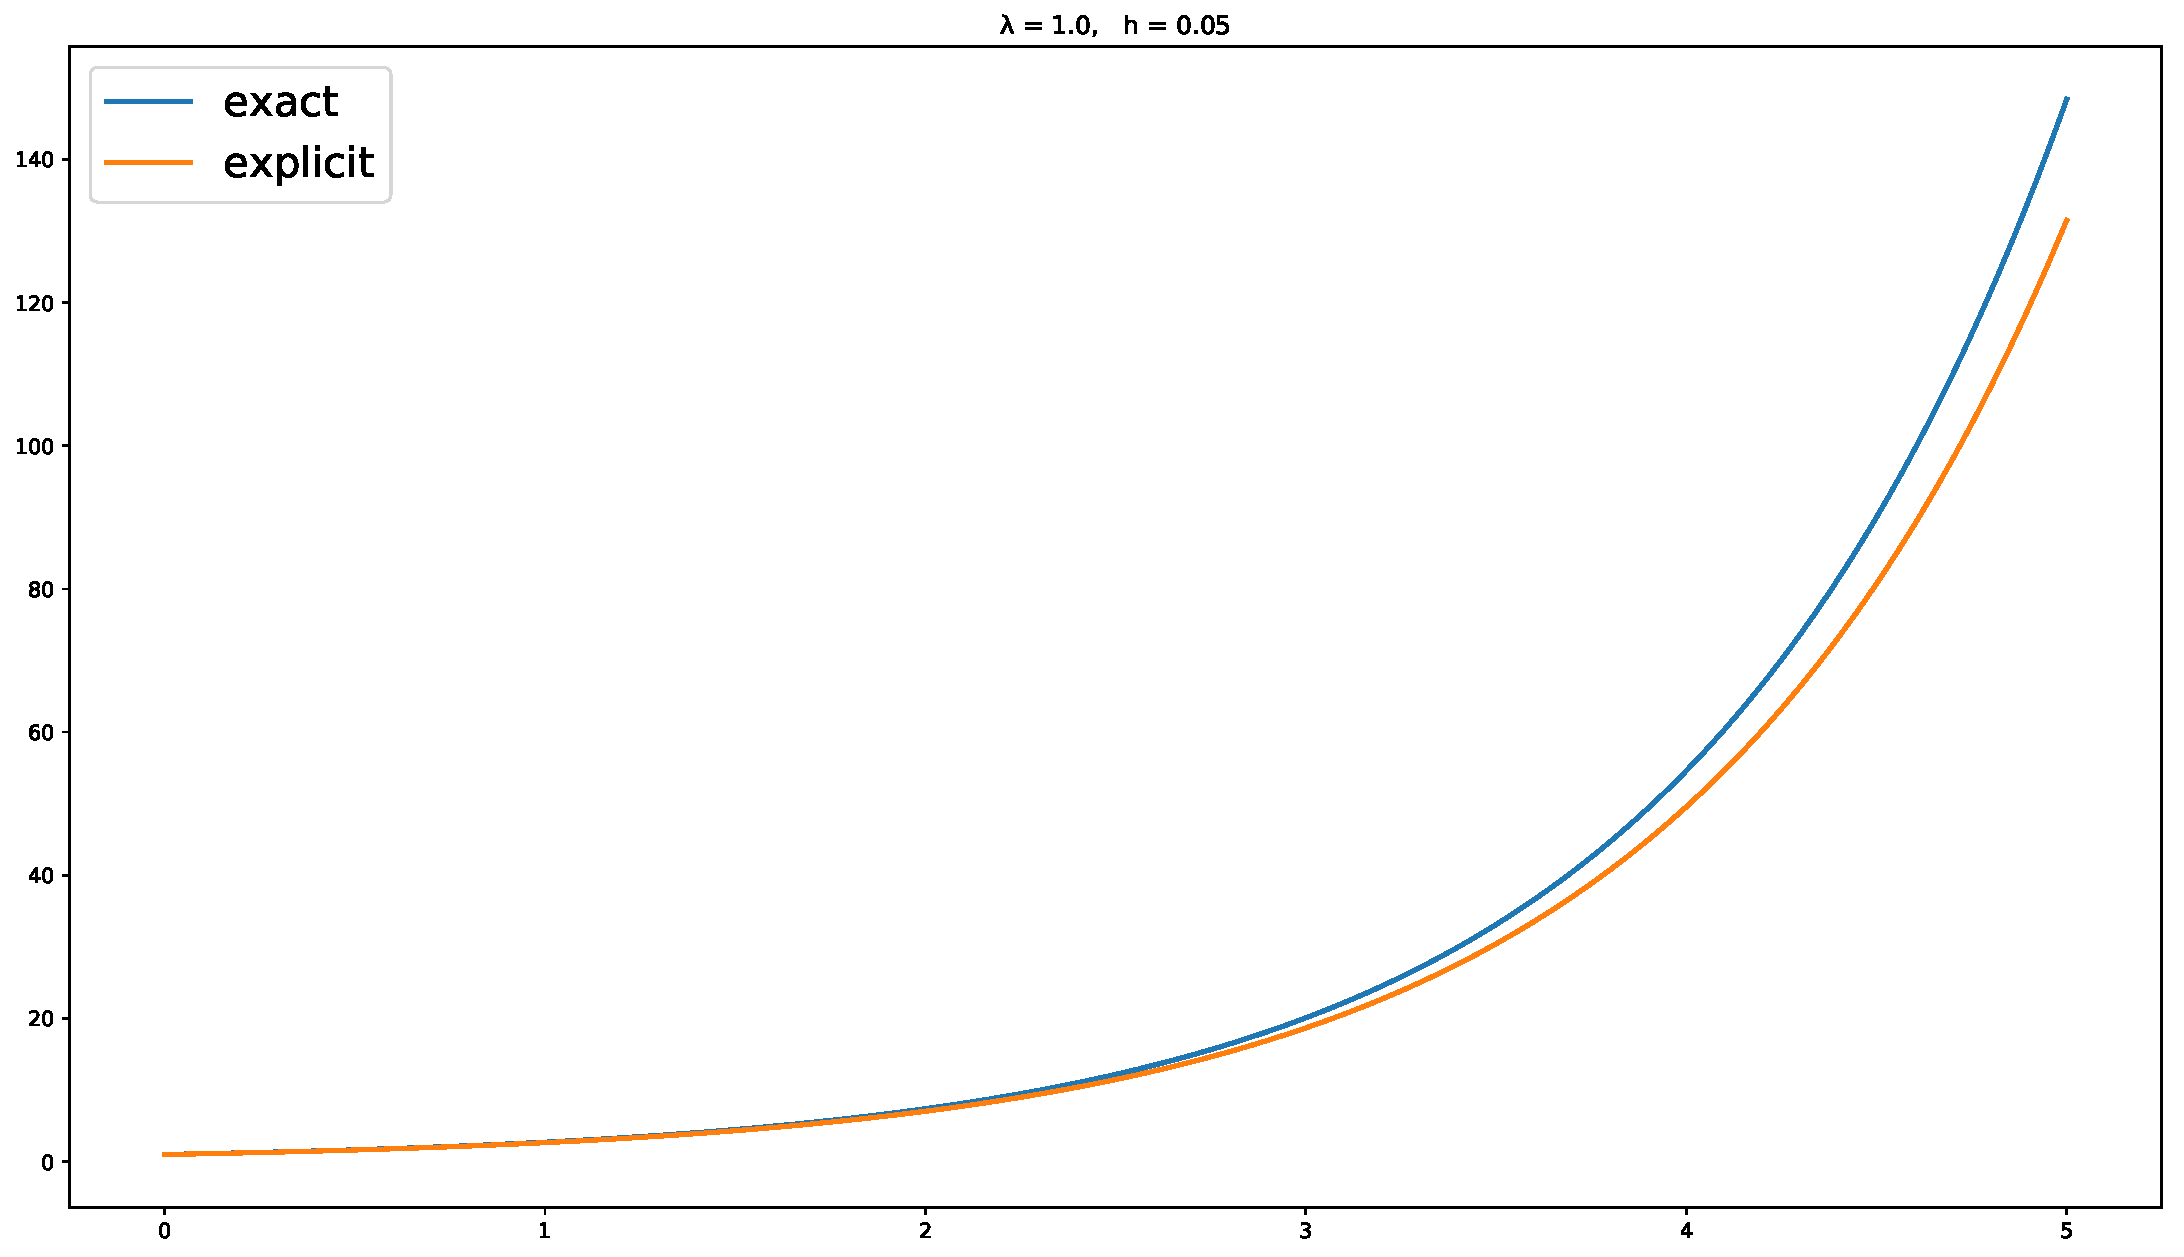
\includegraphics[width=\textwidth]{explicit-euler-lambda-1dot0-h-0dot05}
		\captionof{figure}{$\lambda=1$, $h = 0{,}05$}
	\end{minipage}
	\begin{minipage}{0.49\textwidth}
		\centering
		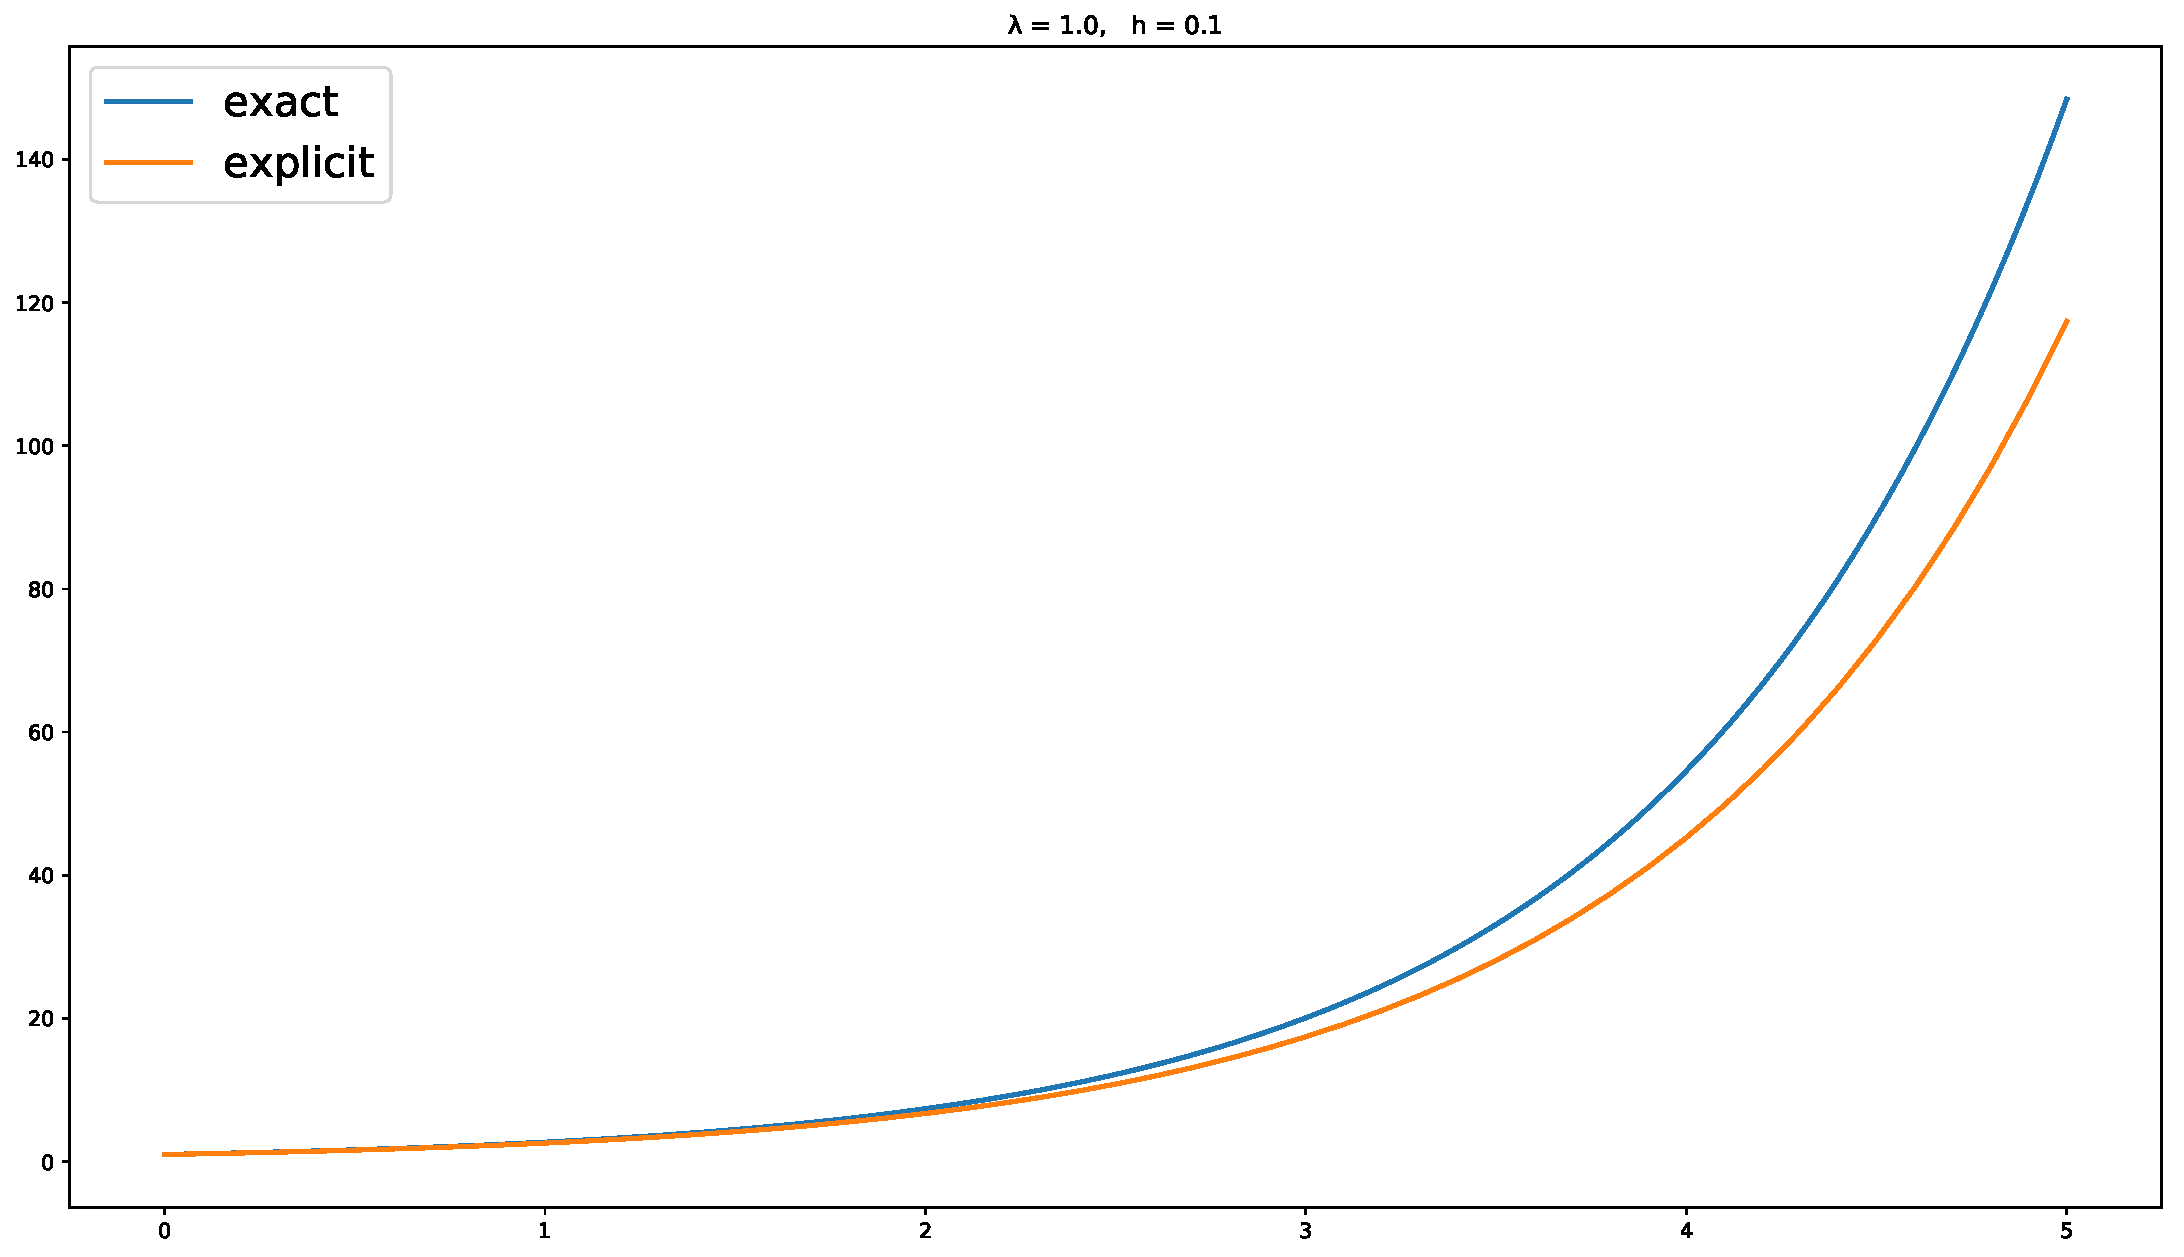
\includegraphics[width=\textwidth]{explicit-euler-lambda-1dot0-h-0dot1}
		\captionof{figure}{$\lambda=1$, $h = 0{,}1$}
	\end{minipage}
\end{center}

\begin{center}
	\begin{minipage}{0.49\textwidth}
		\centering
		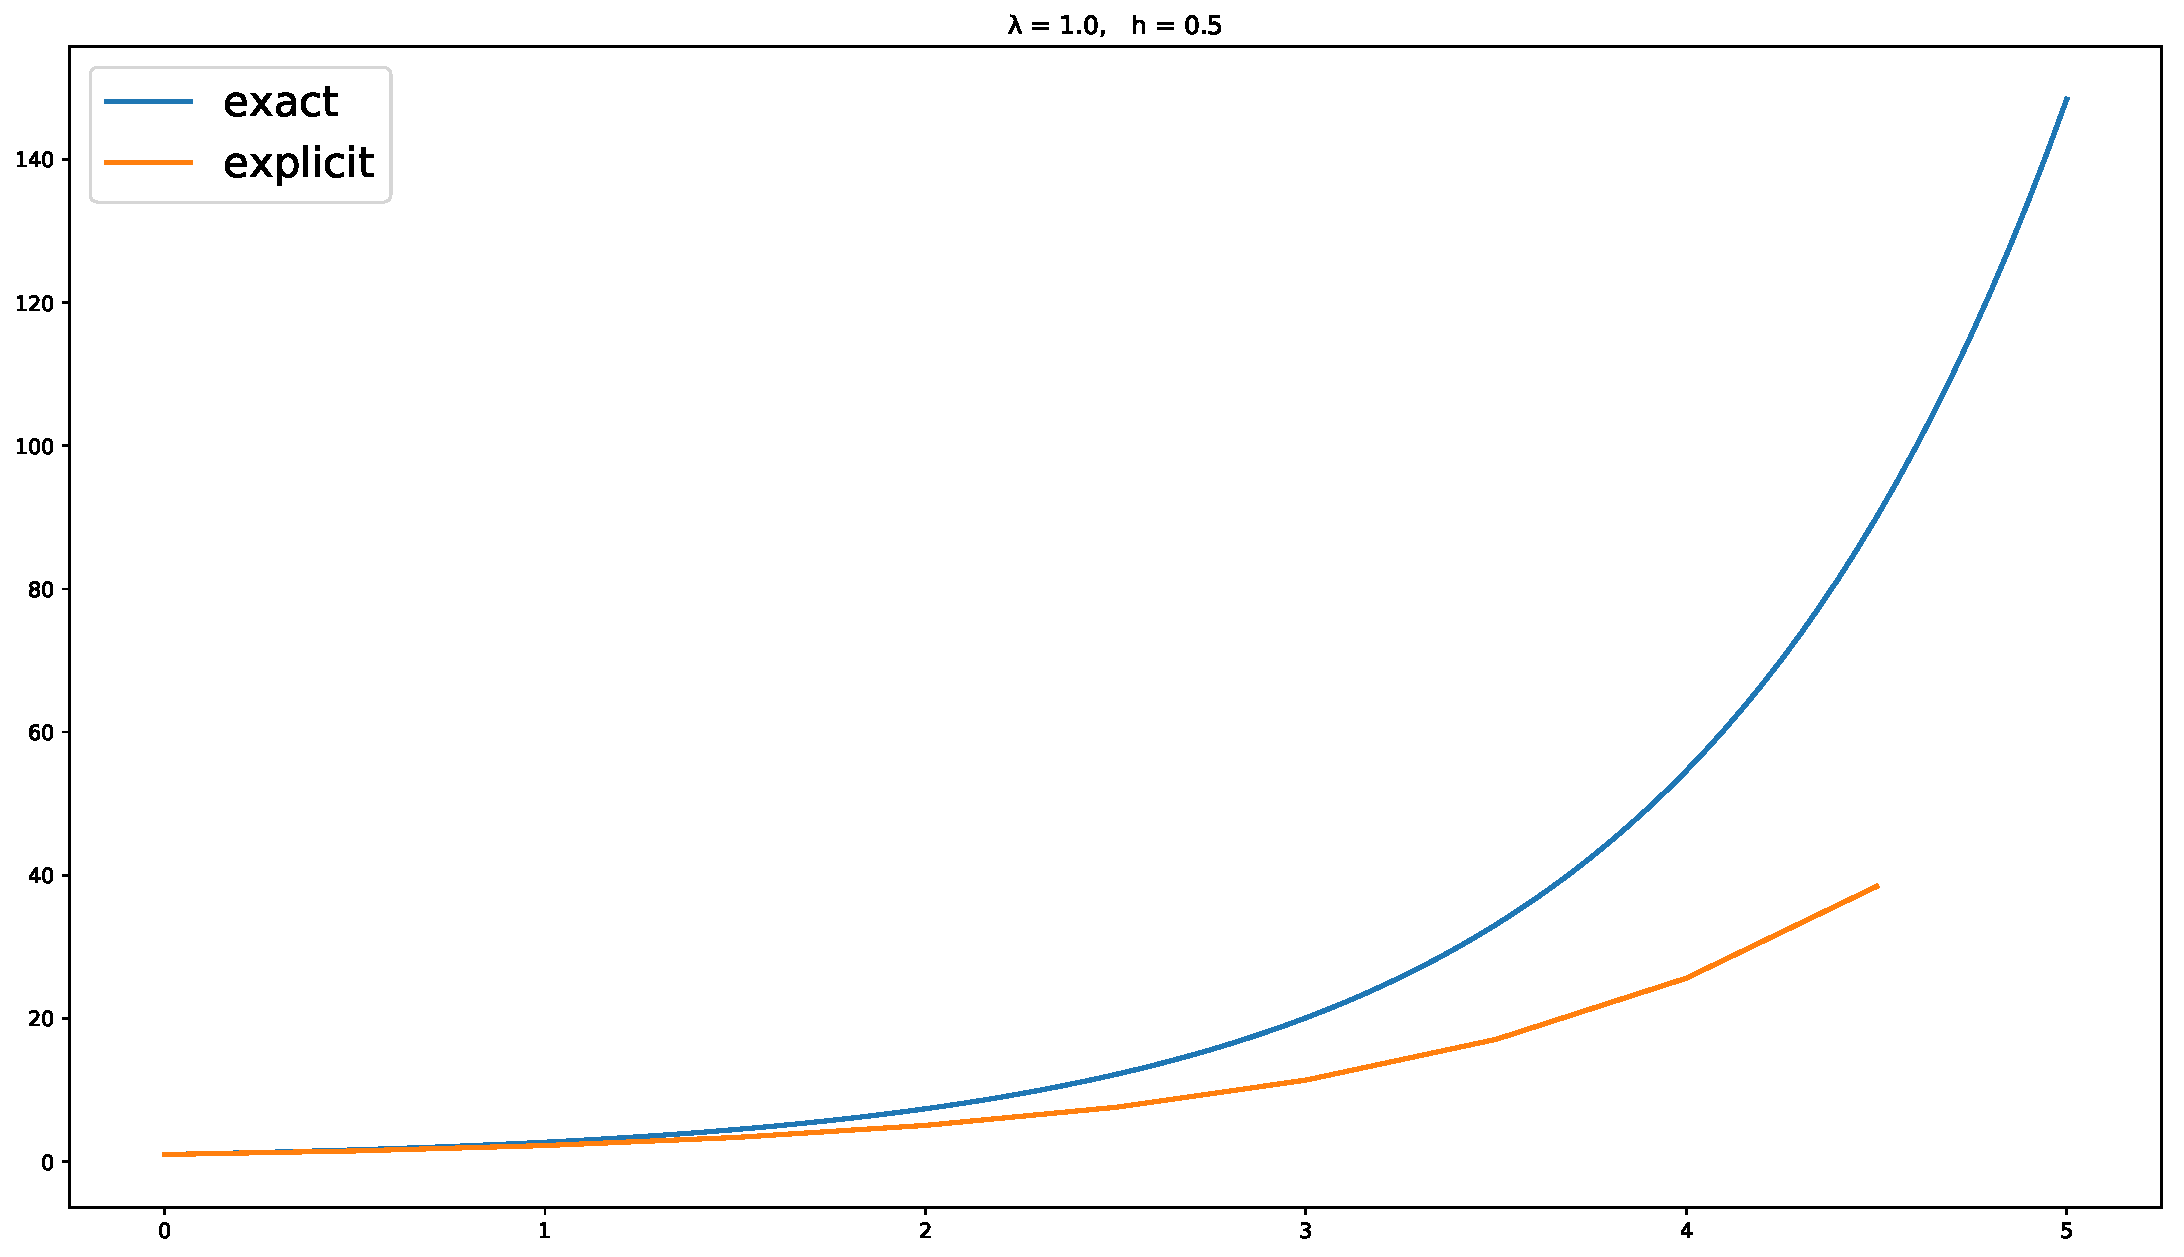
\includegraphics[width=\textwidth]{explicit-euler-lambda-1dot0-h-0dot5}
		\captionof{figure}{$\lambda=1$, $h = 0{,}5$}
	\end{minipage}
	\begin{minipage}{0.49\textwidth}
		\begin{center}
		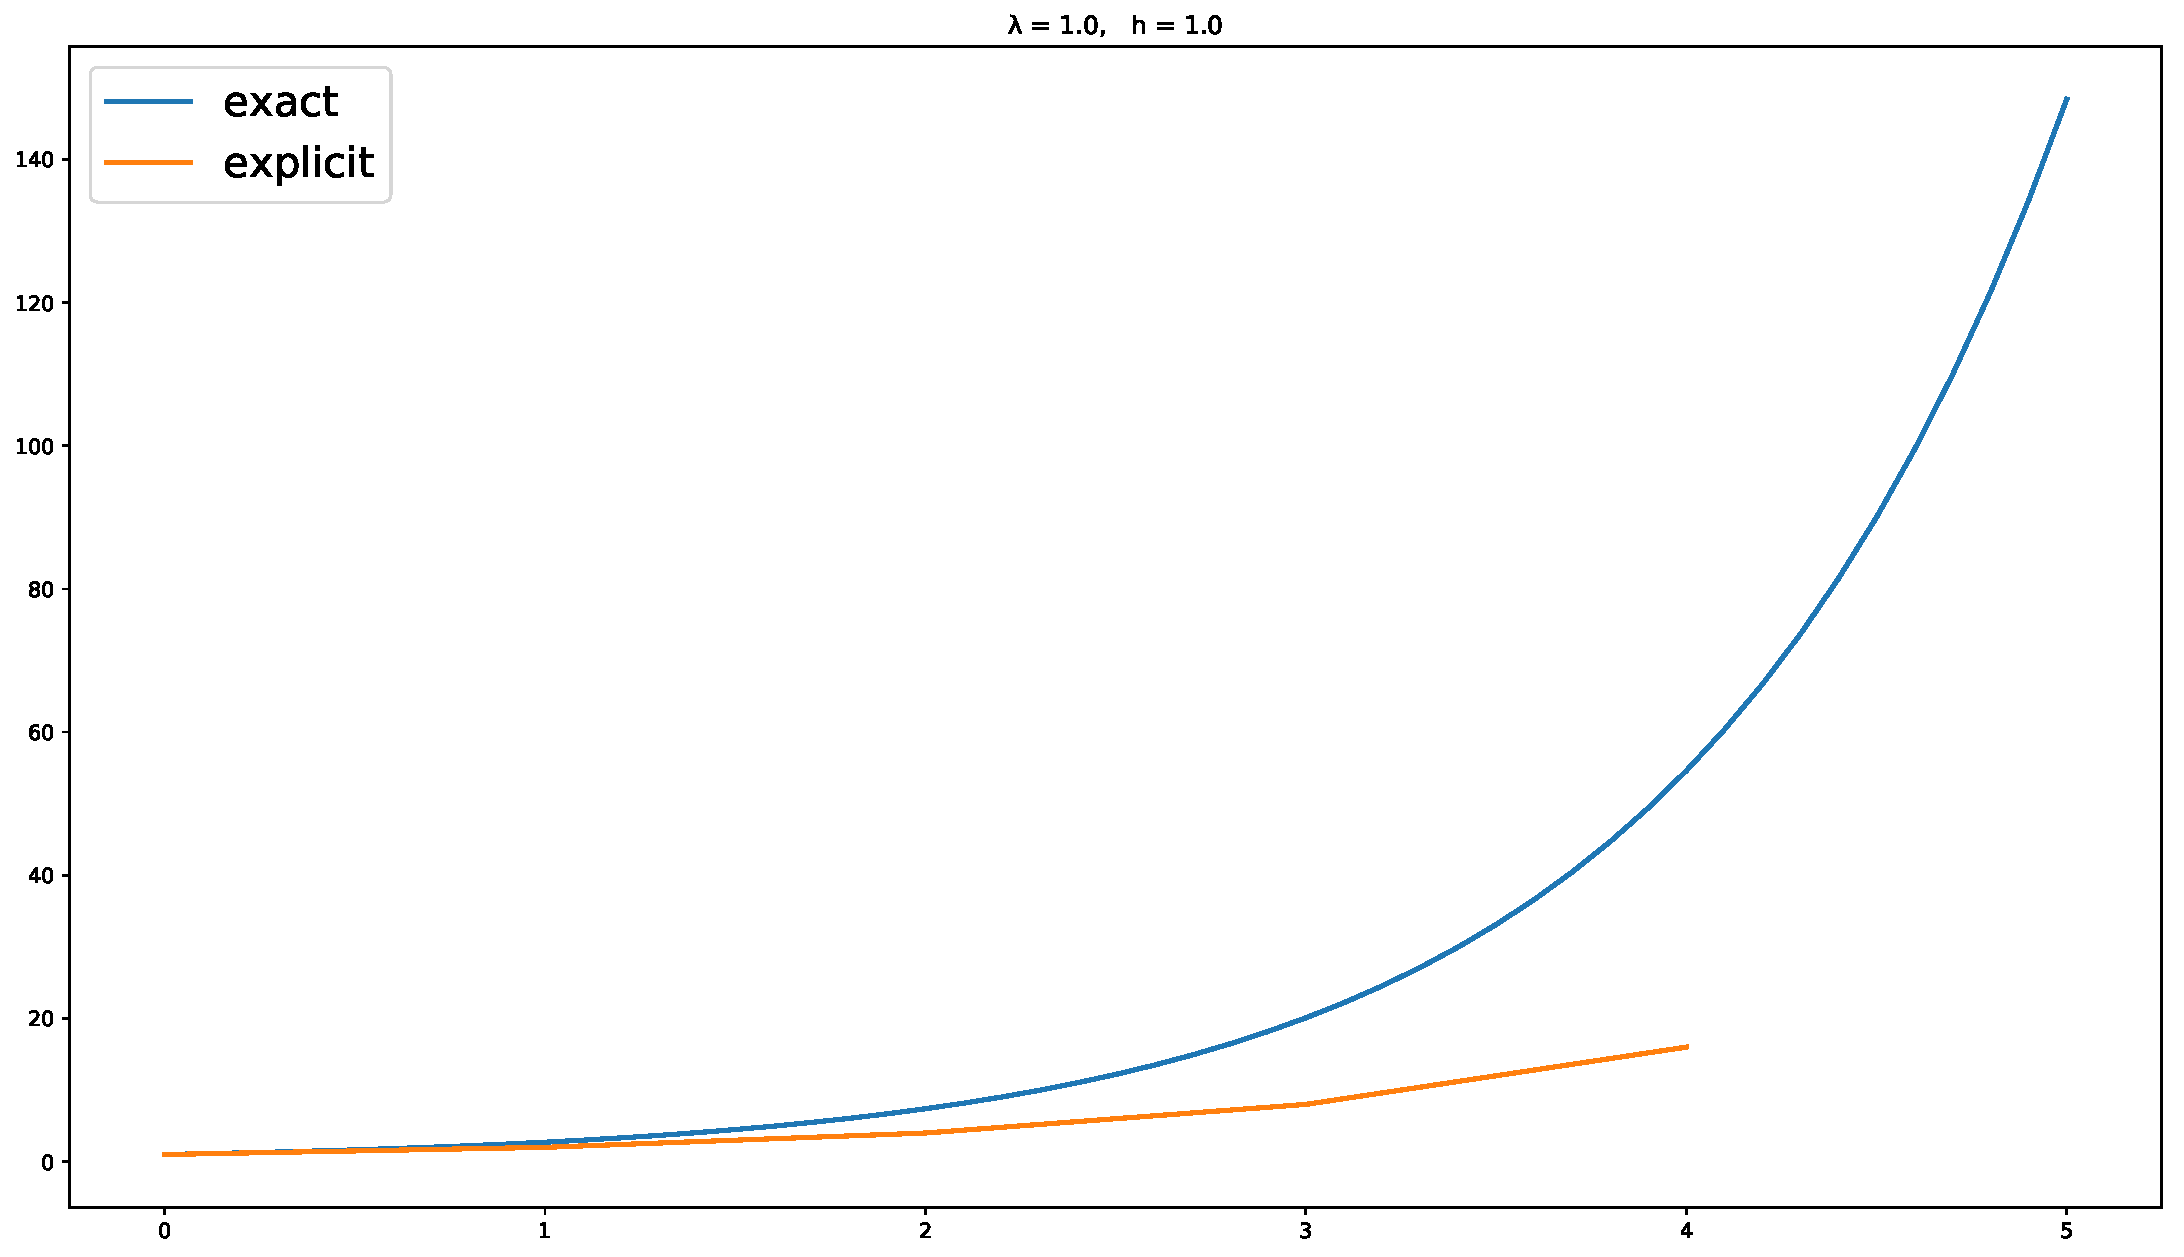
\includegraphics[width=\textwidth]{explicit-euler-lambda-1dot0-h-1dot0}
		\captionof{figure}{$\lambda=1$, $h = 1{,}0$}
		\end{center}
	\end{minipage}
\end{center}


Als nächstes probieren wir ein negatives $\lambda$, hier z.B.\ $\lambda=-1$:

\begin{center}
\begin{minipage}{0.49\textwidth}
	\centering
	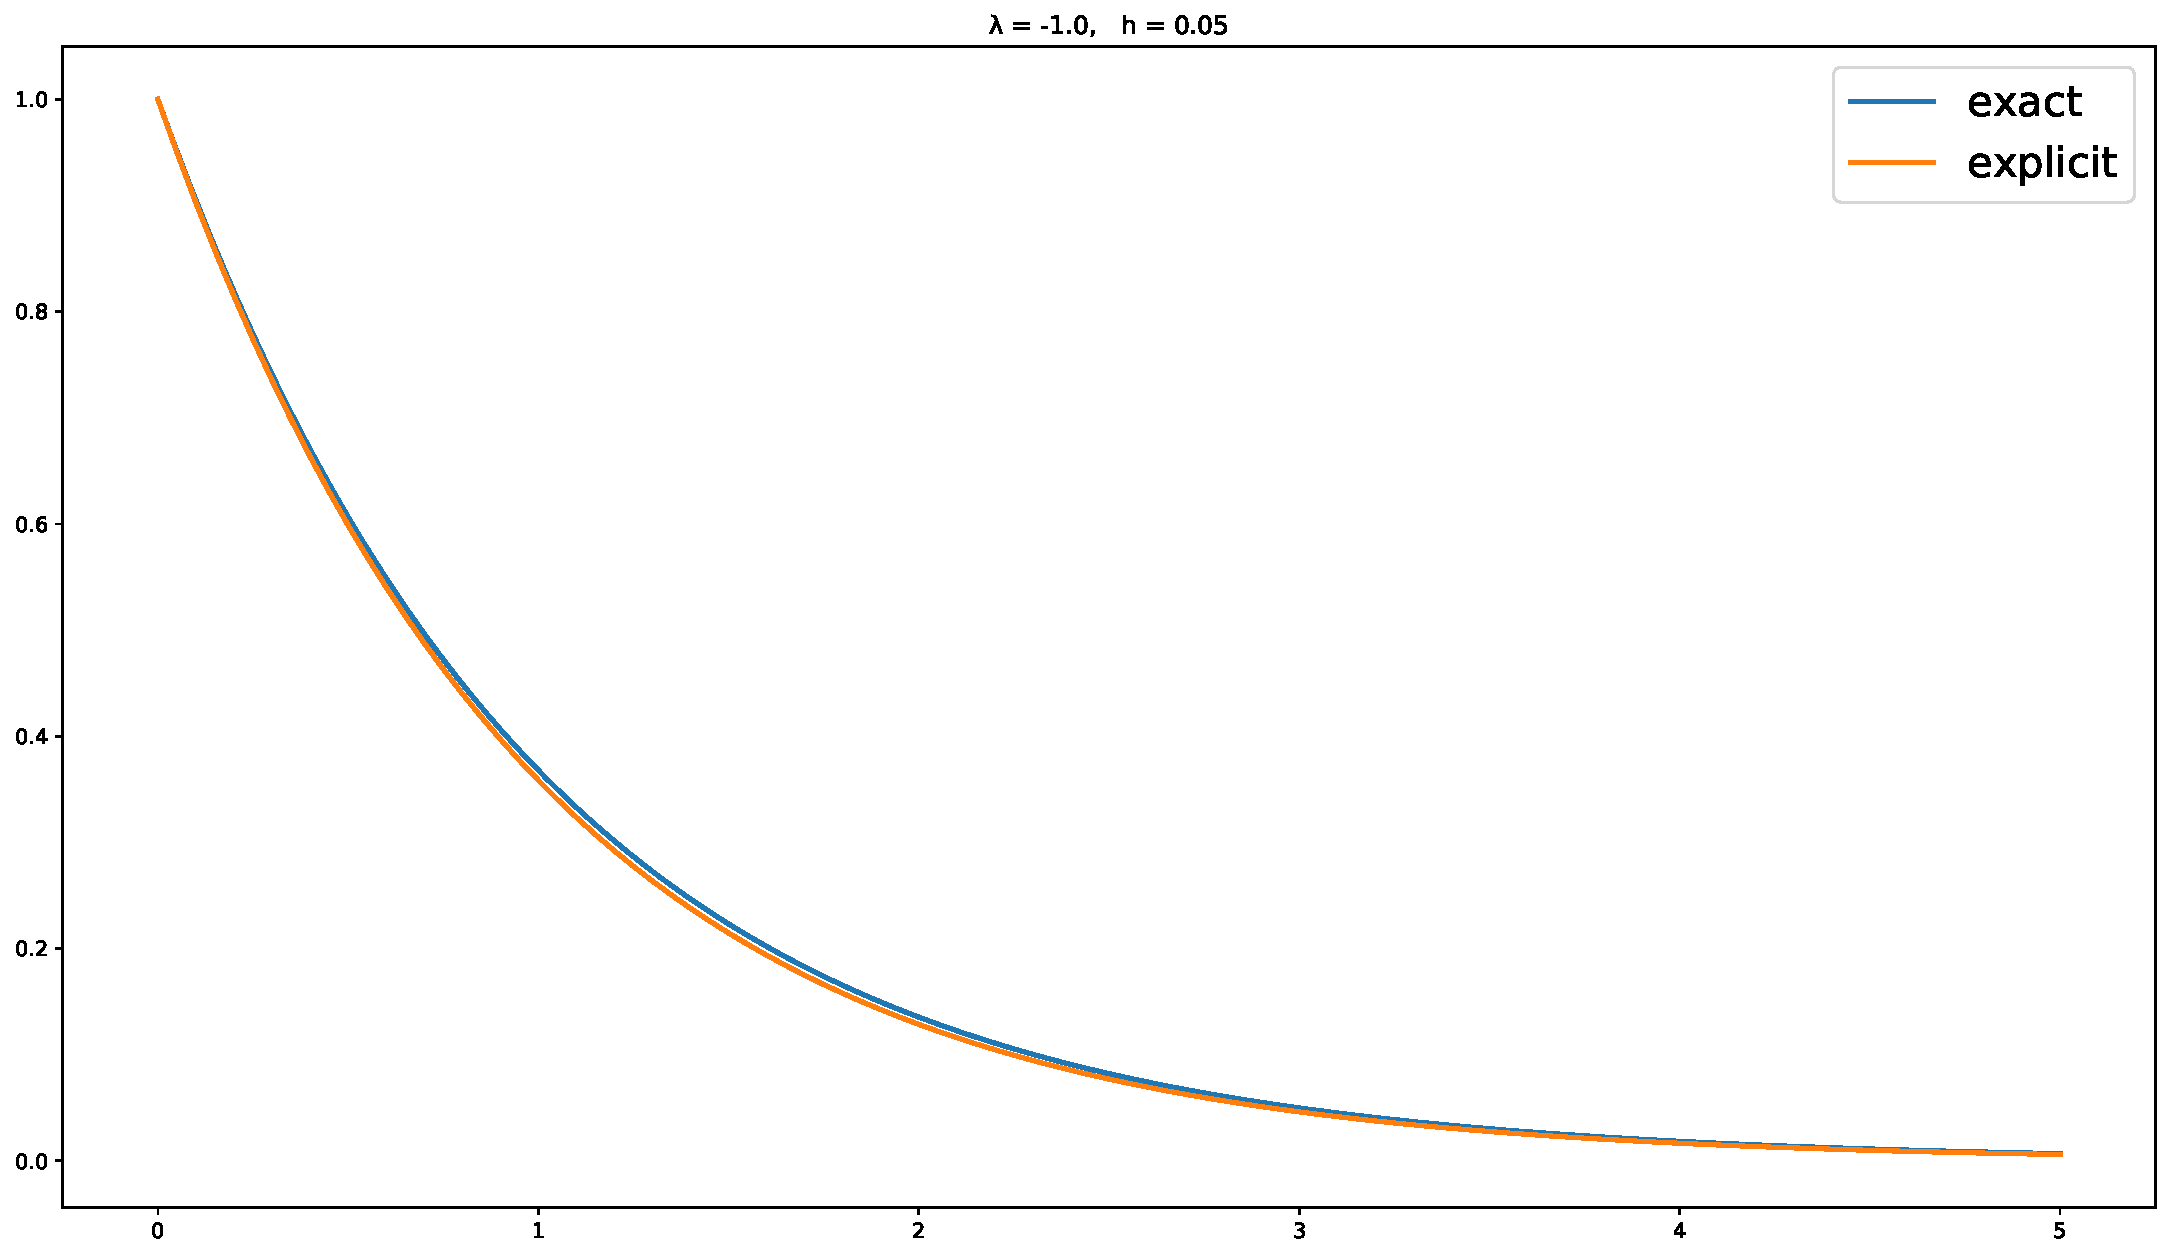
\includegraphics[width=\textwidth]{explicit-euler-lambda--1dot0-h-0dot05} \\
	$\lambda=-1$, $h = 0{,}05$
\end{minipage}
\begin{minipage}{0.49\textwidth}
	\centering
	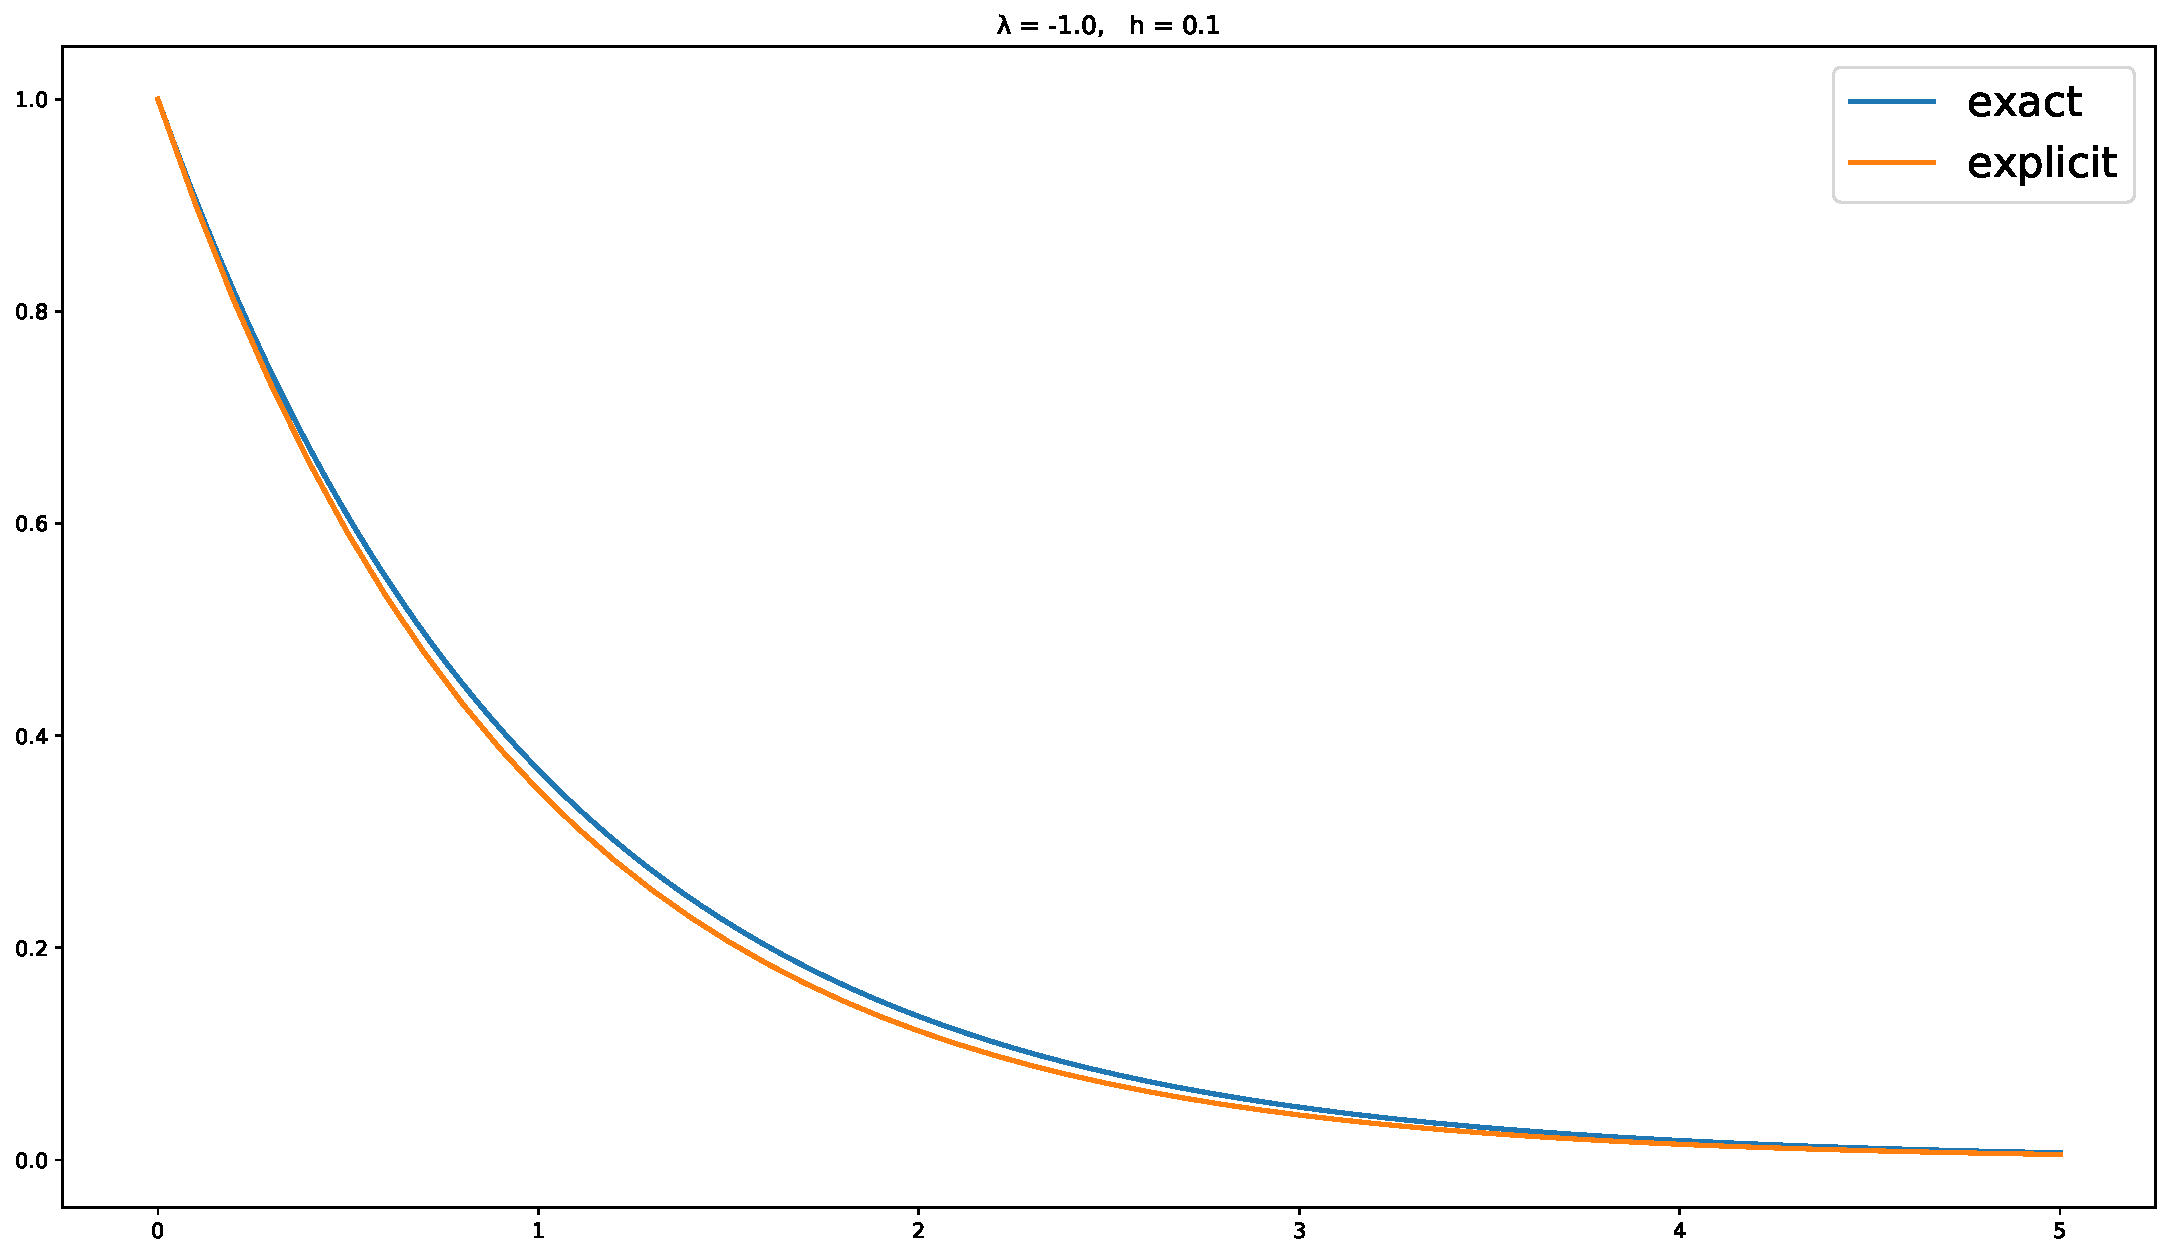
\includegraphics[width=\textwidth]{explicit-euler-lambda--1dot0-h-0dot1} \\
	$\lambda=-1$, $h = 0{,}1$
\end{minipage}
\end{center}

\begin{center}
	\begin{minipage}{0.49\textwidth}
		\centering
		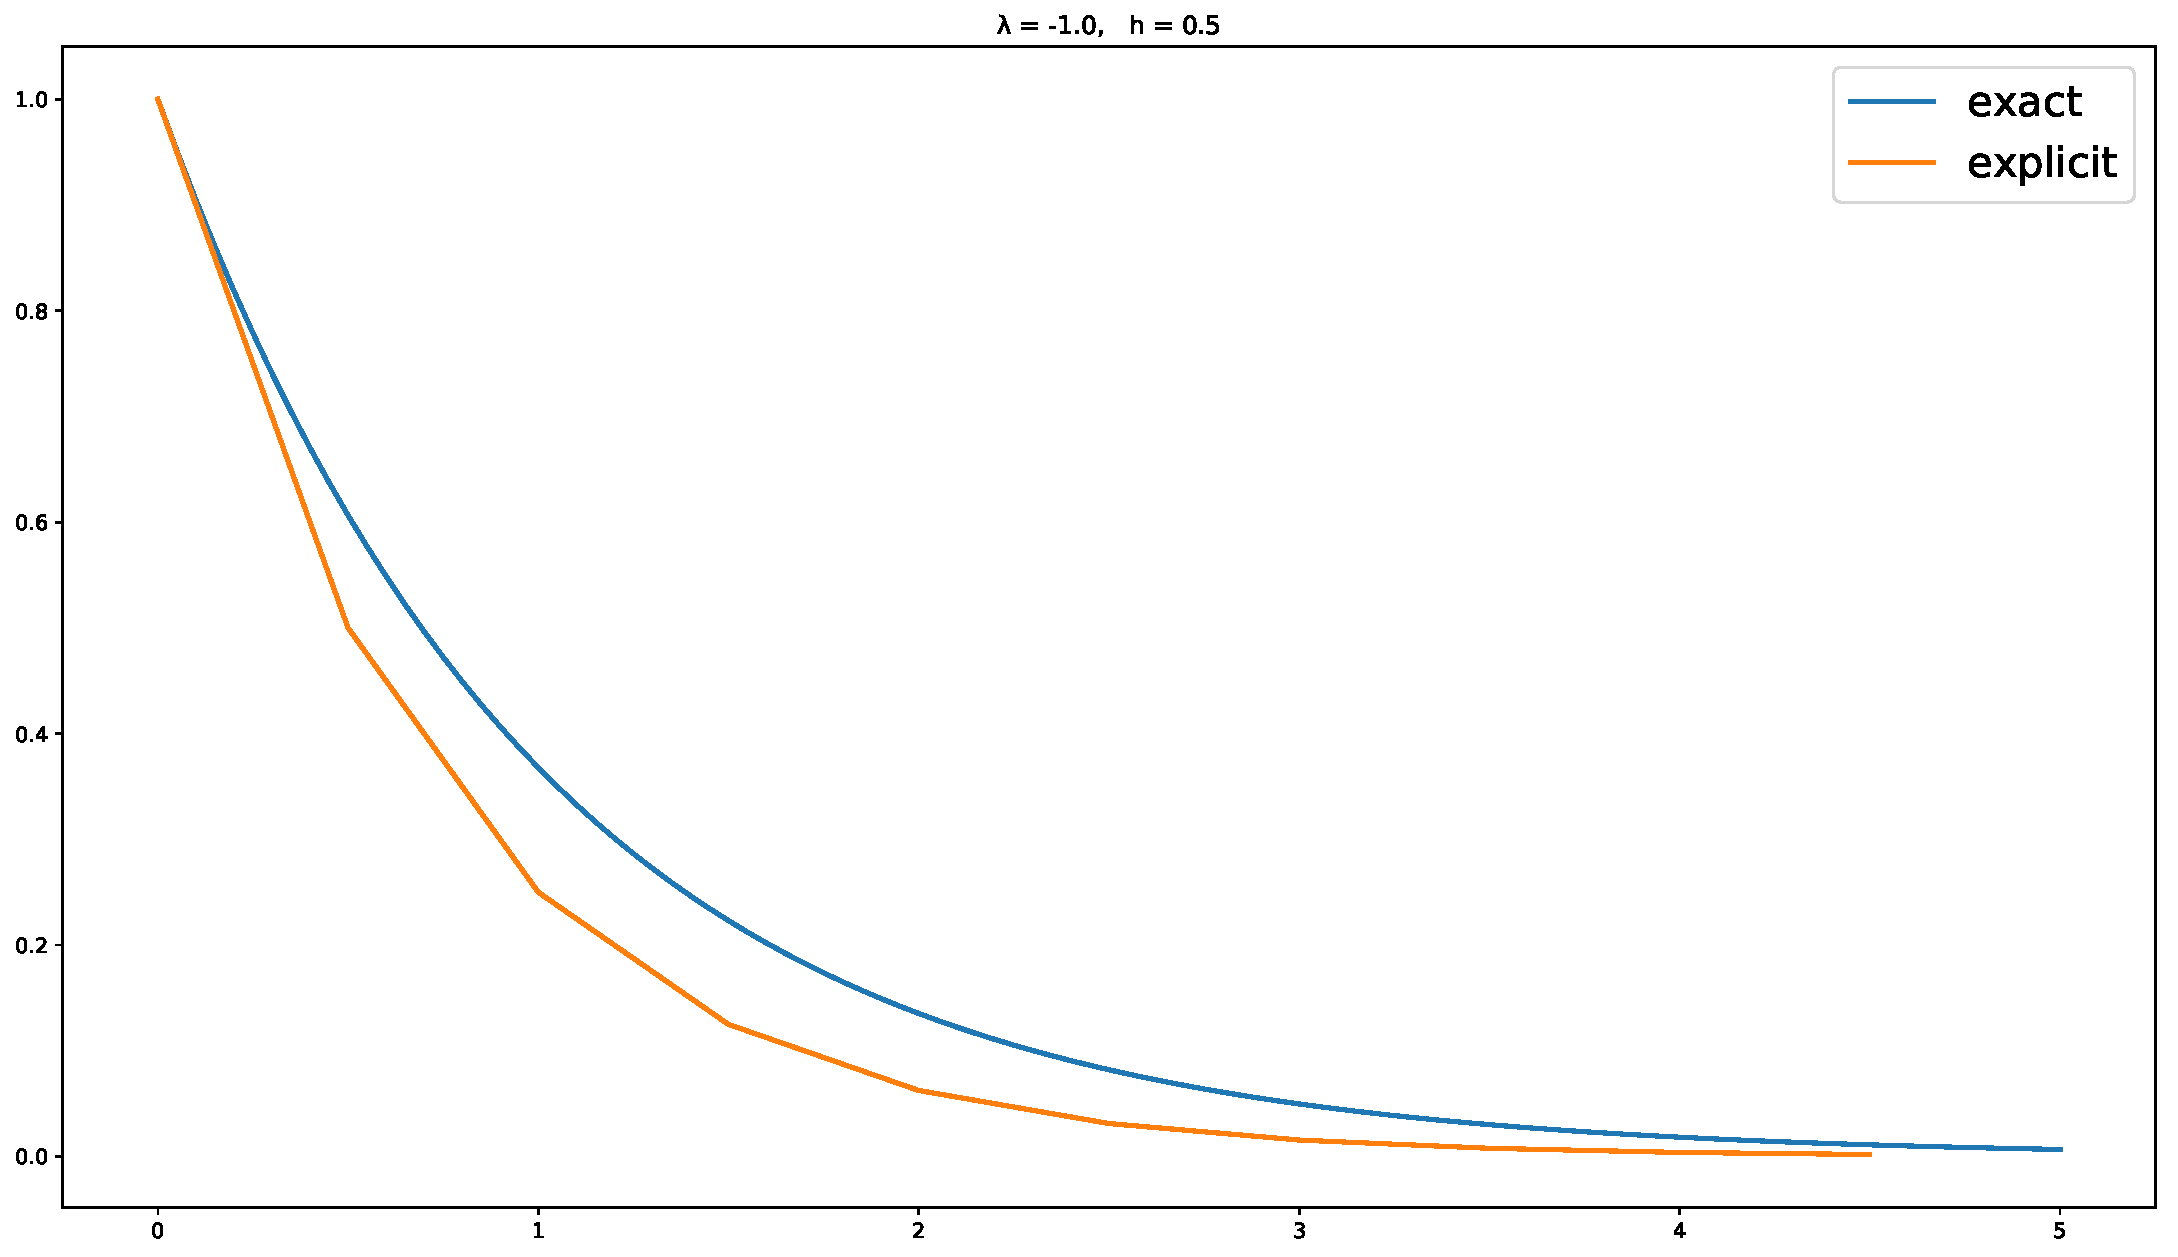
\includegraphics[width=\textwidth]{explicit-euler-lambda--1dot0-h-0dot5} \\
		$\lambda=-1$, $h = 0{,}5$
	\end{minipage}
	\begin{minipage}{0.49\textwidth}
		\centering
		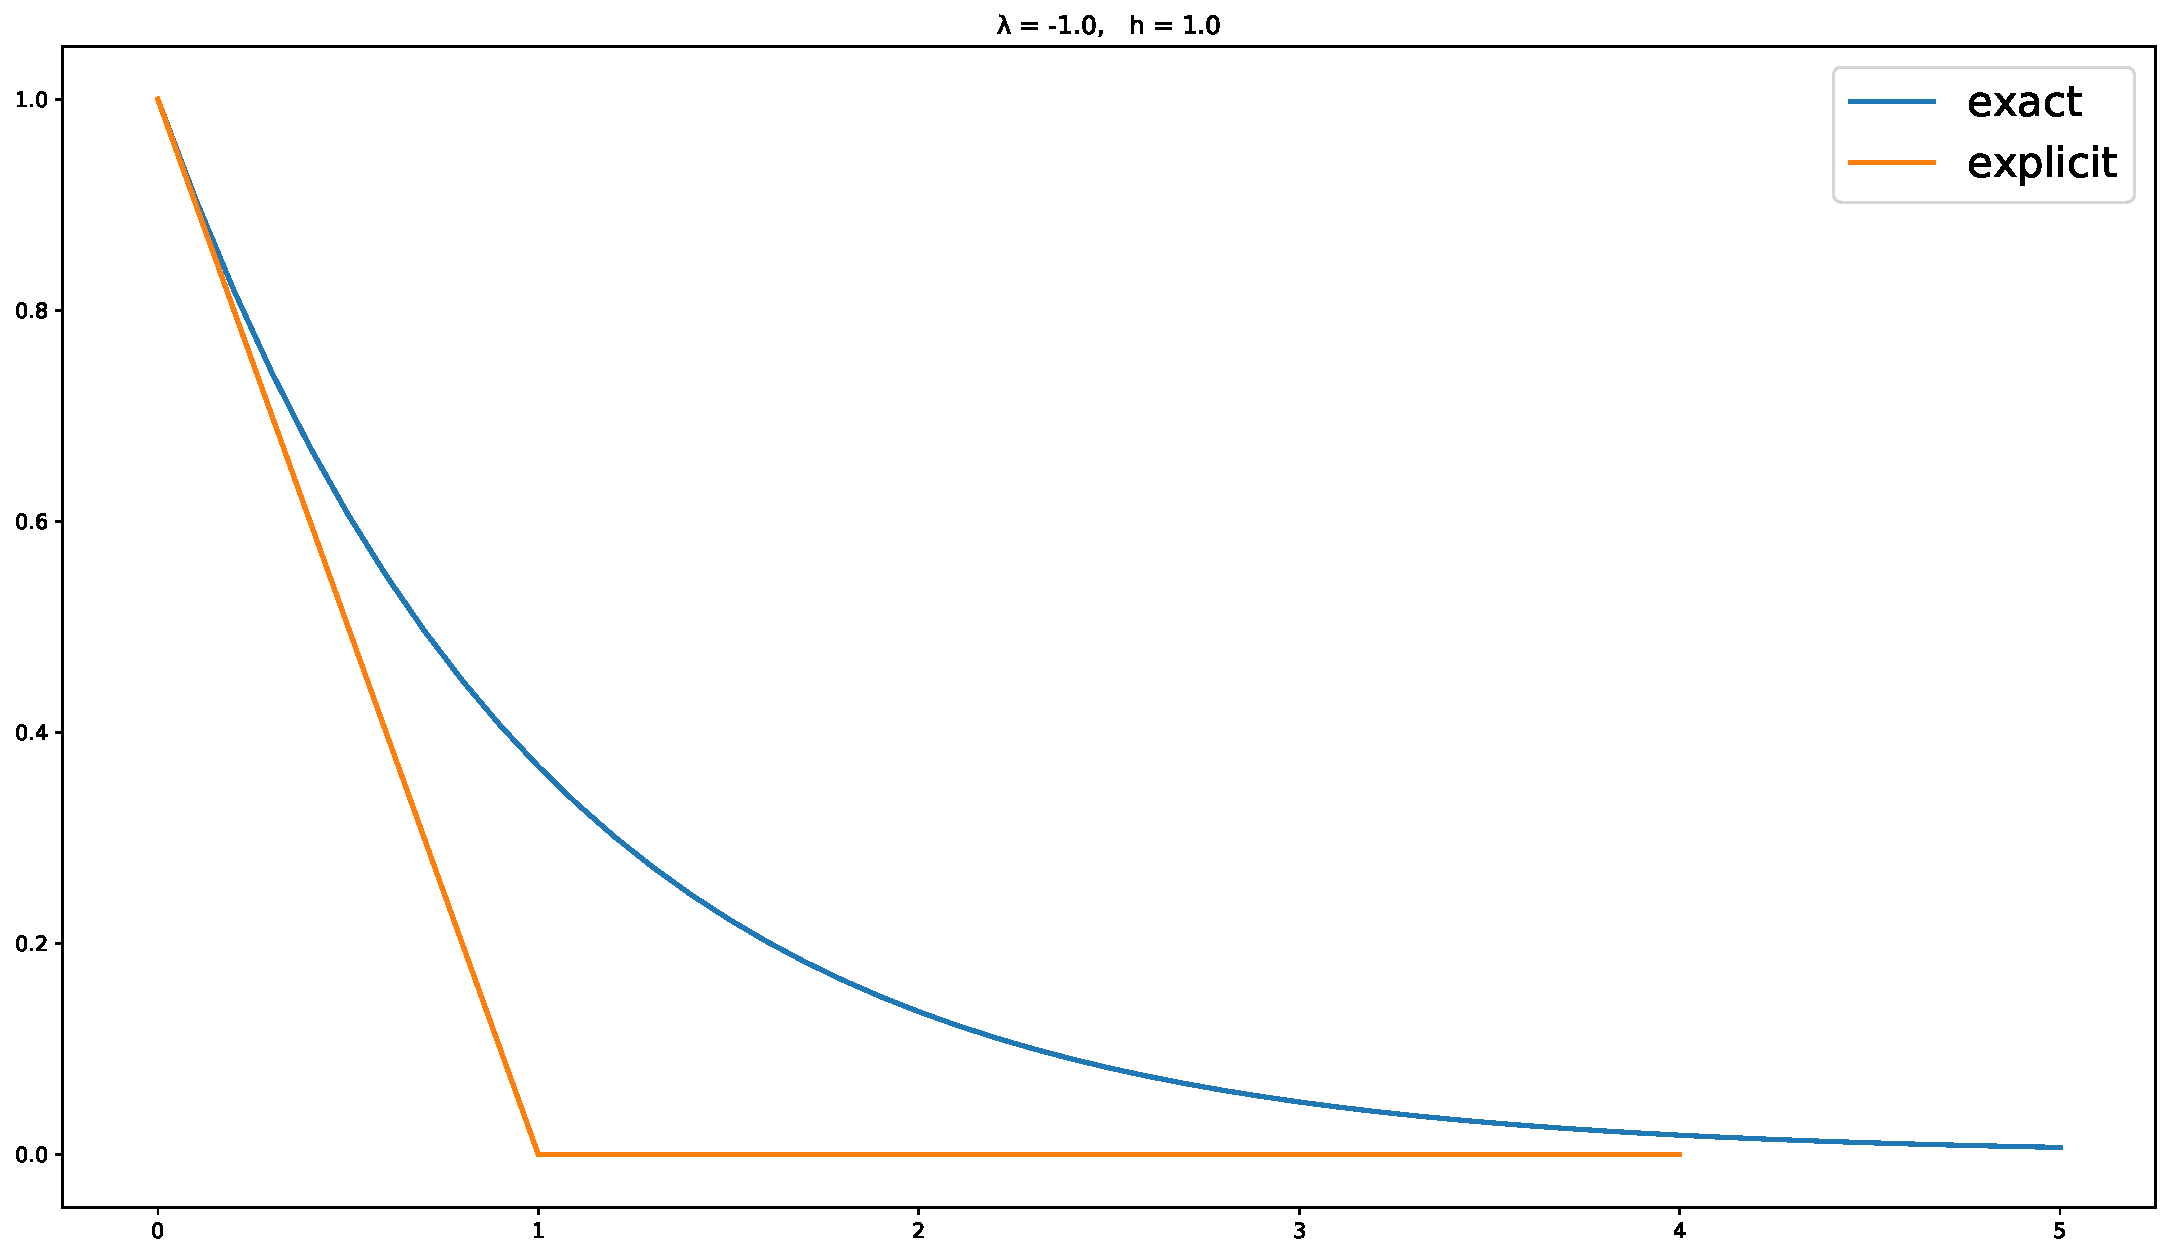
\includegraphics[width=\textwidth]{explicit-euler-lambda--1dot0-h-1dot0} \\
		$\lambda=-1$, $h = 1{,}0$
	\end{minipage}
\end{center}

\bigskip

Die letzte Rechnung sieht ein wenig seltsam aus, aber der Rest ist okay.

Probieren wir noch $\lambda = -5$:

\begin{center}
	\begin{minipage}{0.49\textwidth}
		\centering
		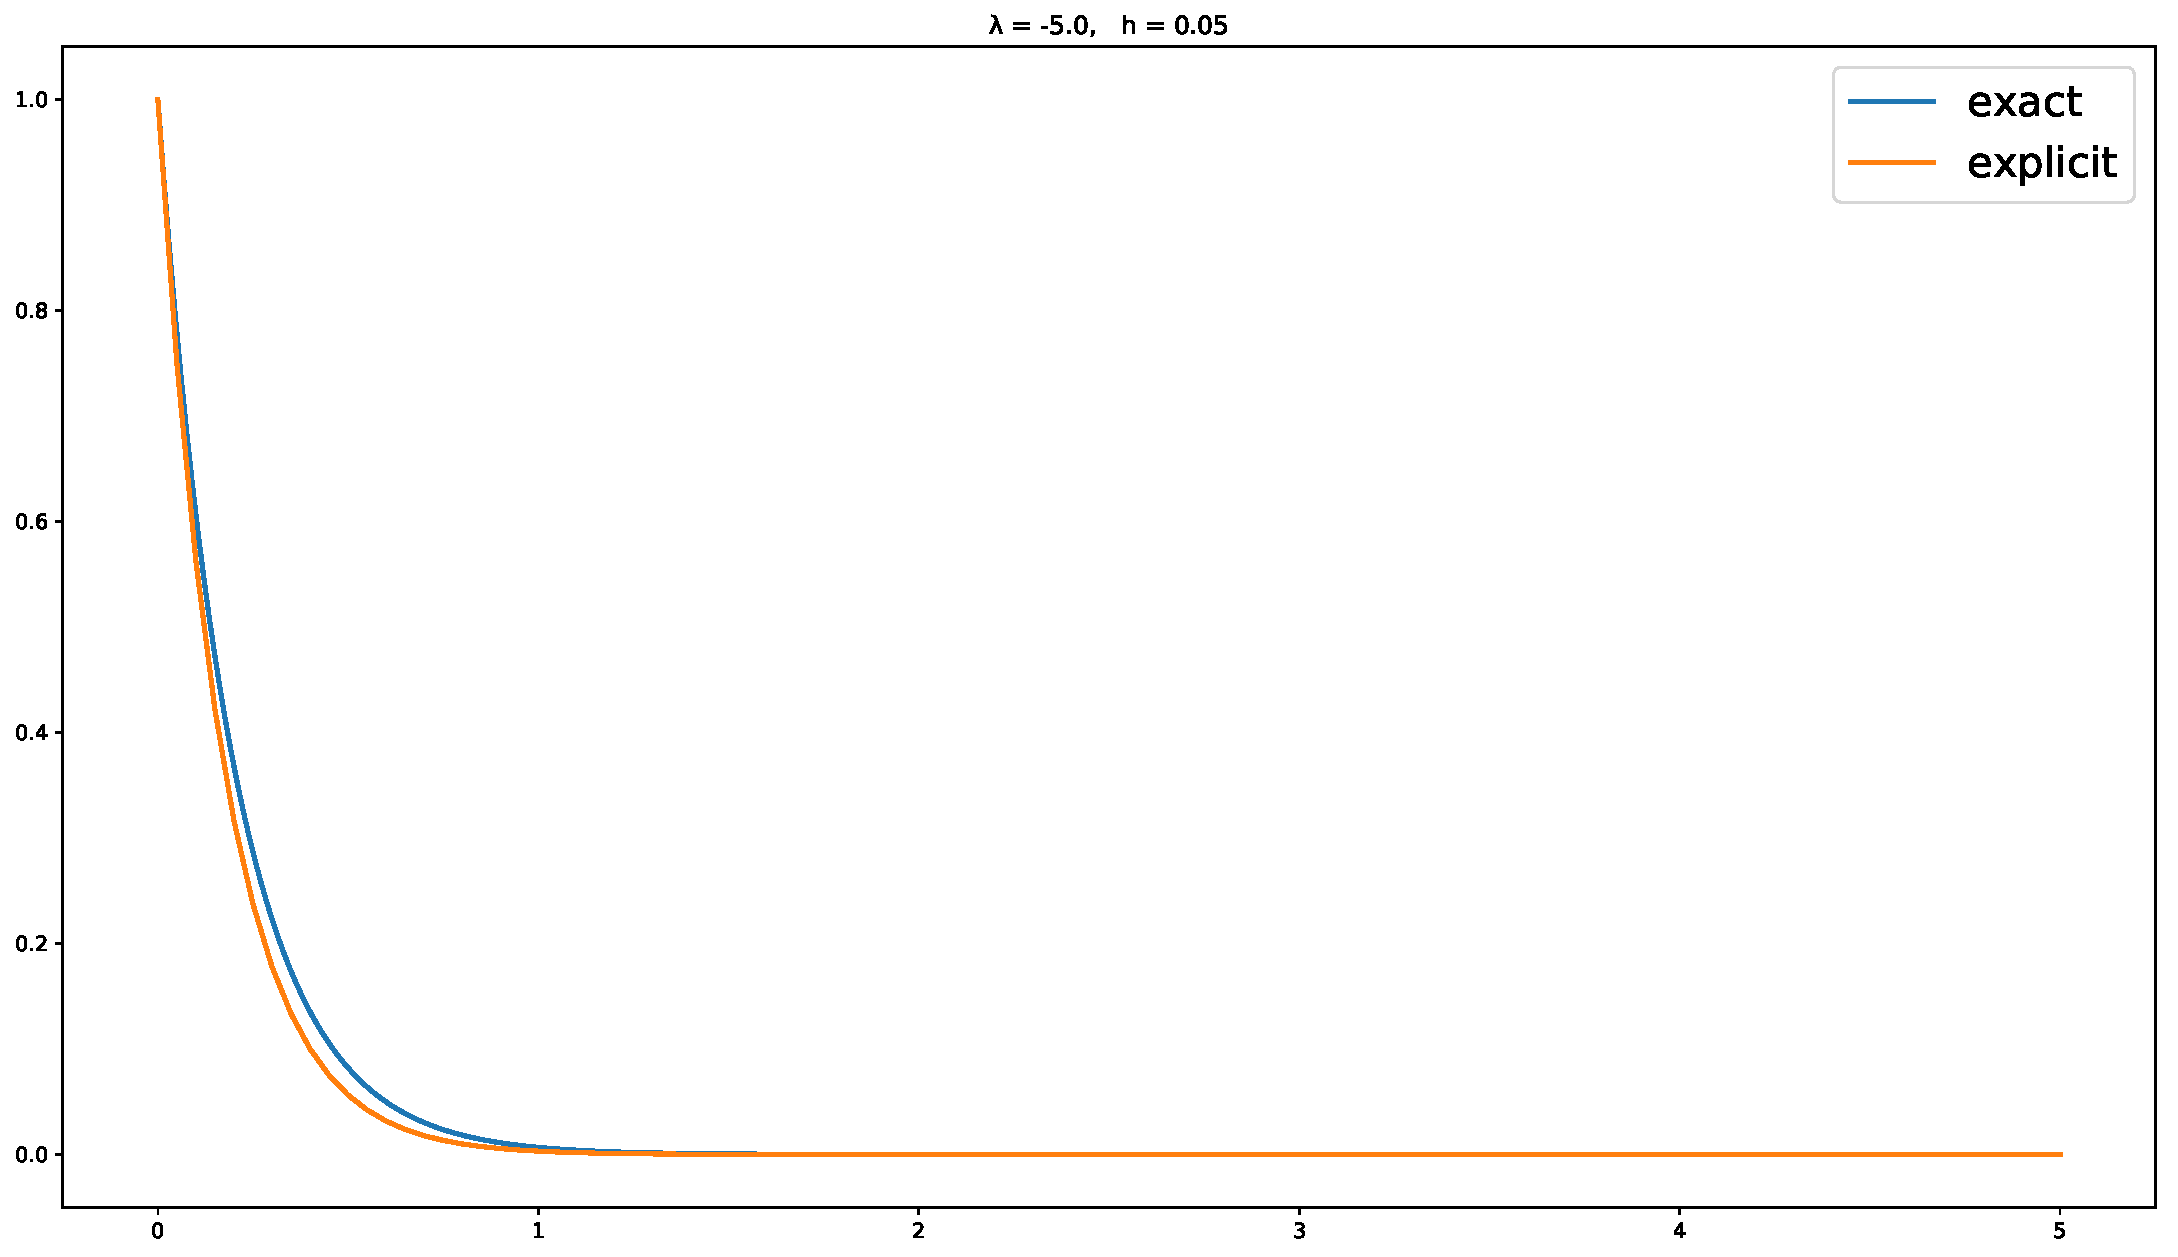
\includegraphics[width=\textwidth]{explicit-euler-lambda--5dot0-h-0dot05} \\
		$\lambda=-5$, $h = 0{,}05$
	\end{minipage}
	\begin{minipage}{0.49\textwidth}
		\centering
		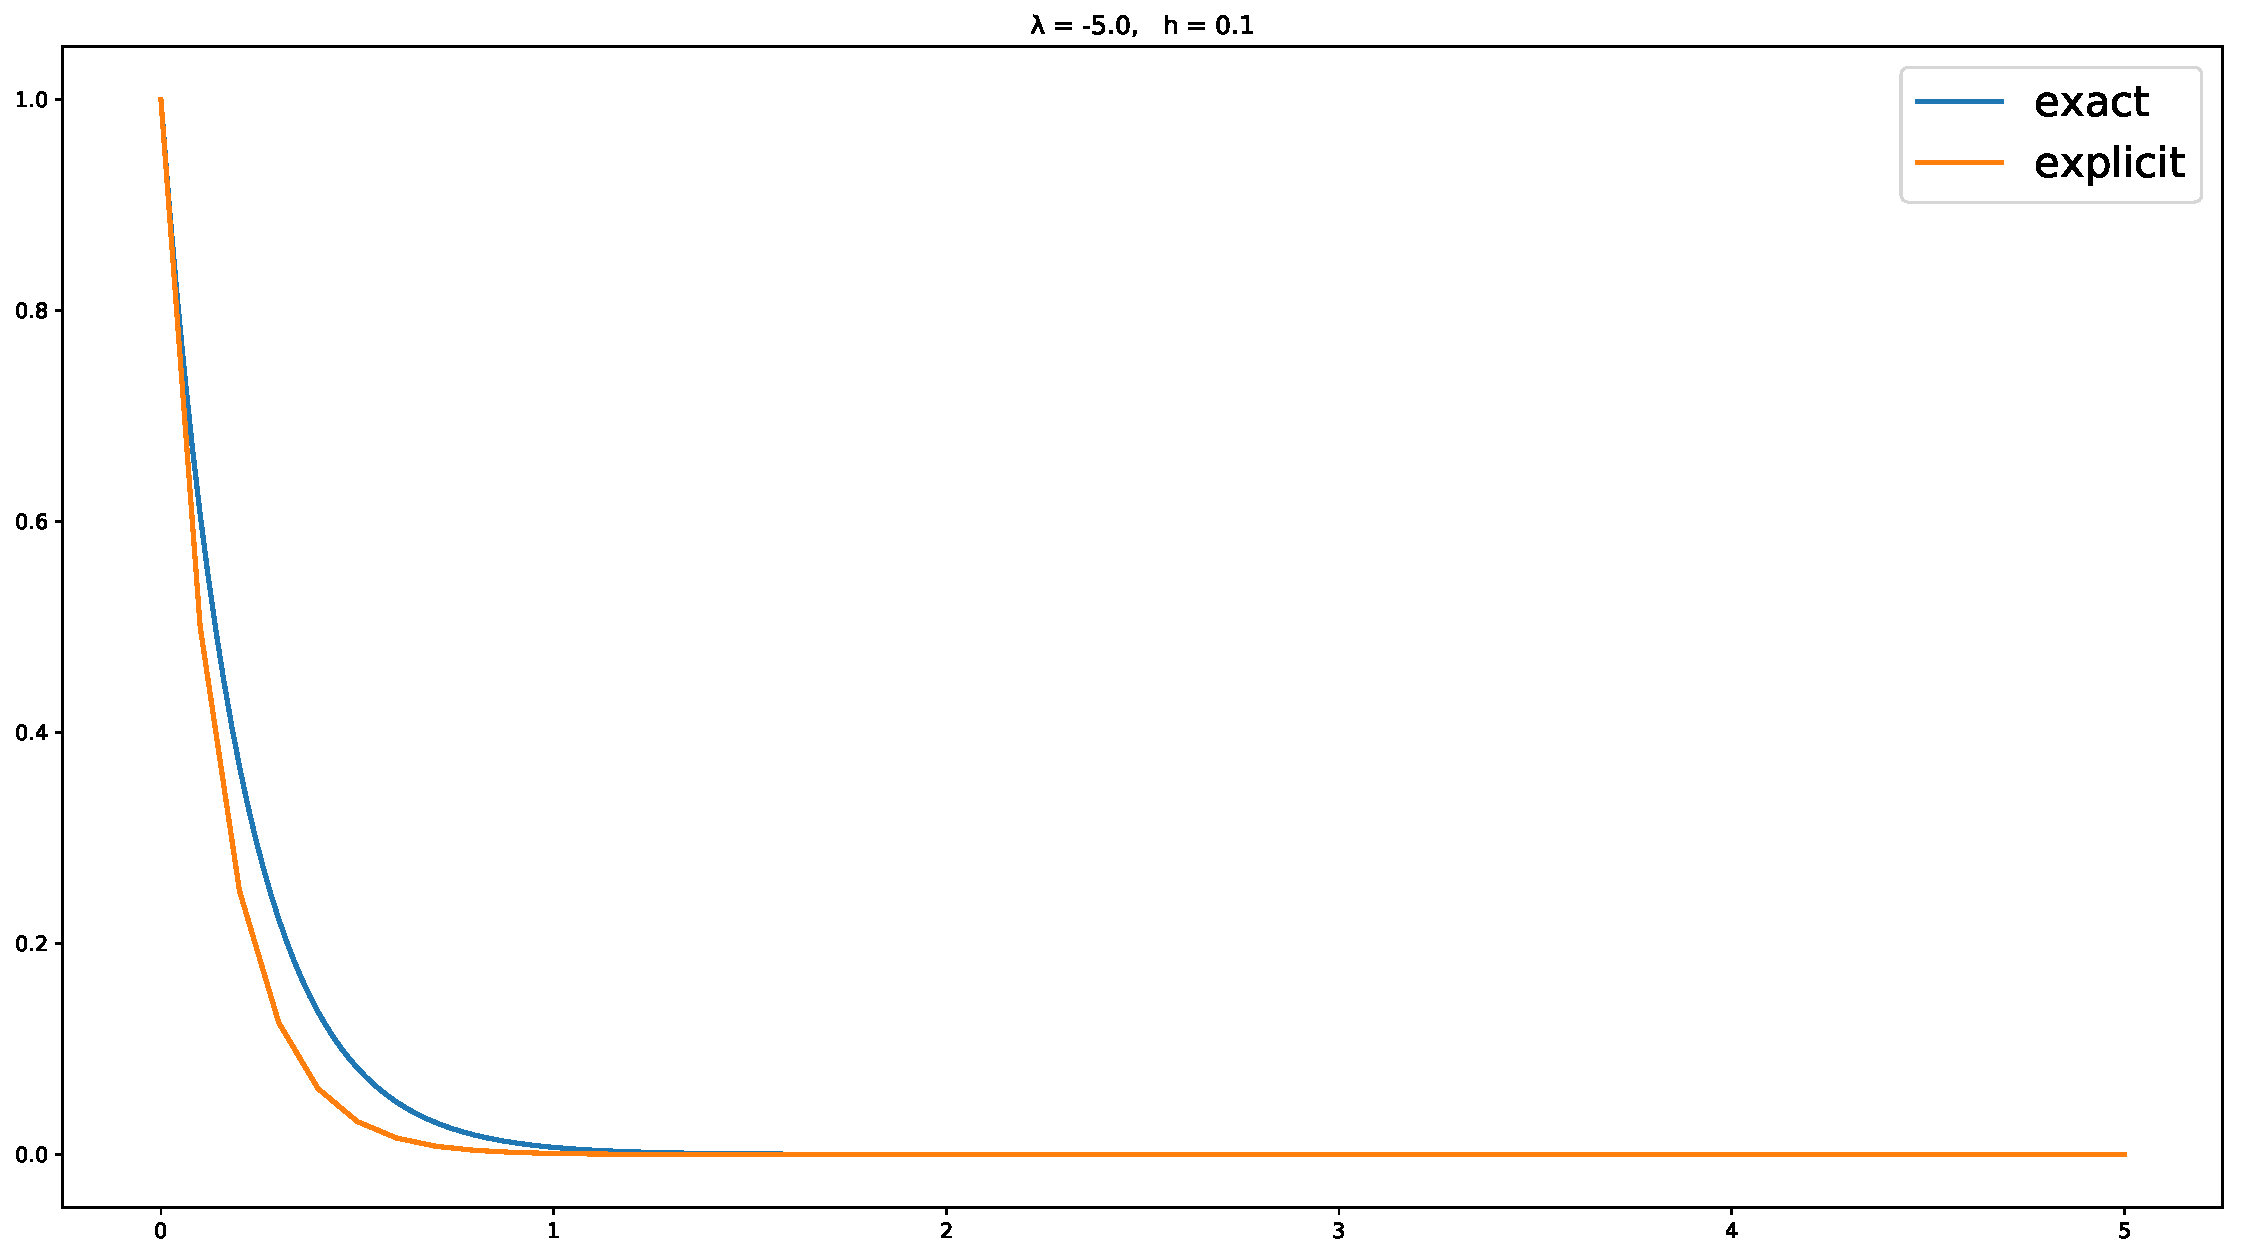
\includegraphics[width=\textwidth]{explicit-euler-lambda--5dot0-h-0dot1} \\
		$\lambda=-5$, $h = 0{,}1$
	\end{minipage}
\end{center}

\begin{center}
	\begin{minipage}{0.49\textwidth}
		\centering
		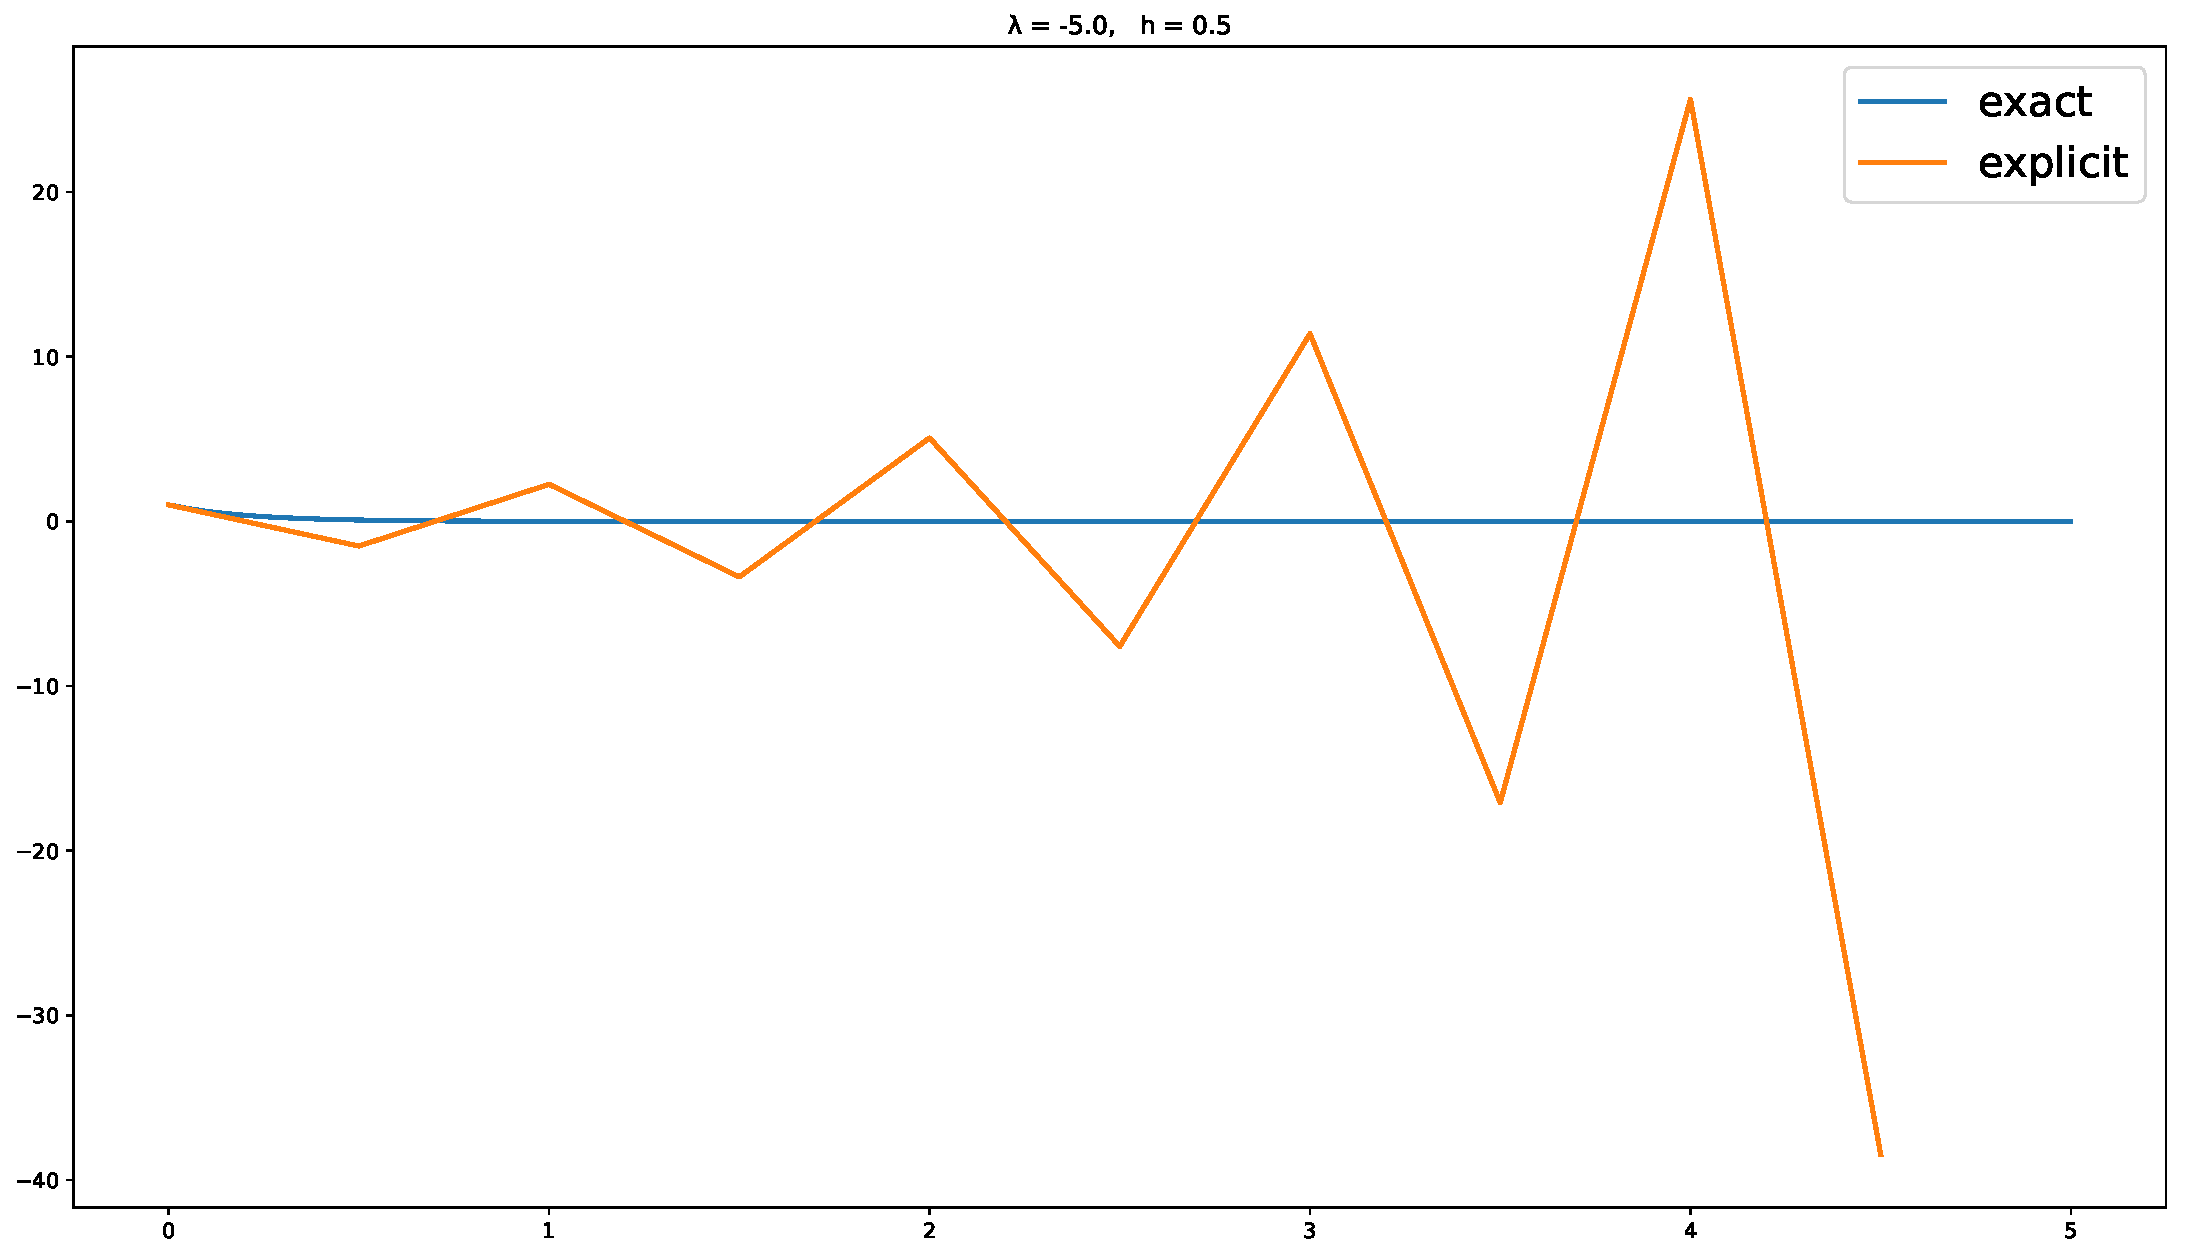
\includegraphics[width=\textwidth]{explicit-euler-lambda--5dot0-h-0dot5} \\
		$\lambda=-5$, $h = 0{,}5$
	\end{minipage}
	\begin{minipage}{0.49\textwidth}
		\centering
		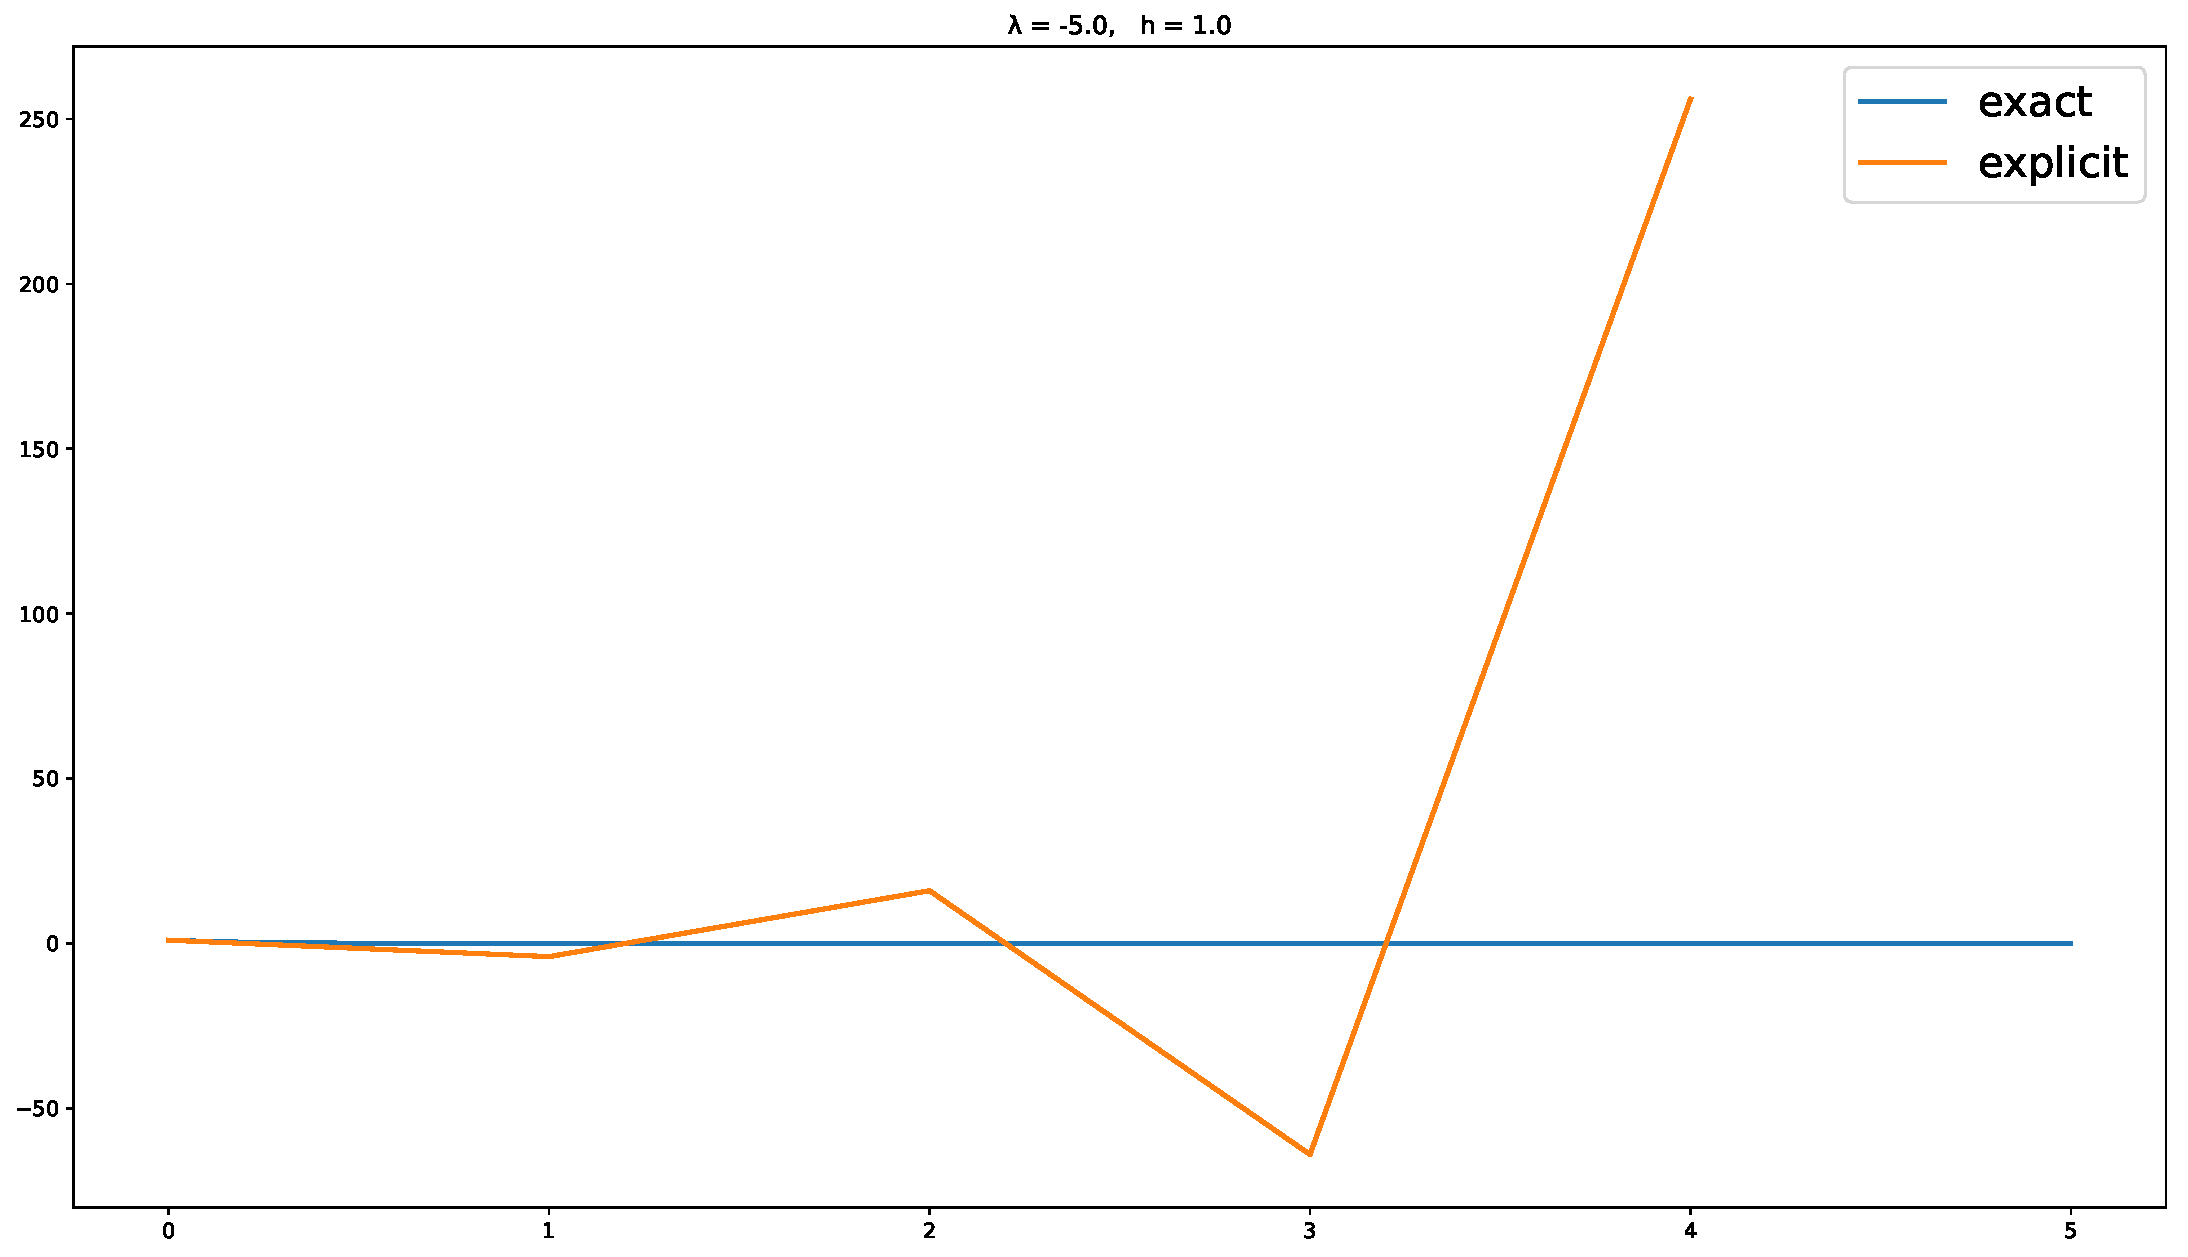
\includegraphics[width=\textwidth]{explicit-euler-lambda--5dot0-h-1dot0} \\
		$\lambda=-5$, $h = 1{,}0$
	\end{minipage}
\end{center}
%
Fazit:
\begin{itemize}[topsep=-\parskip, nolistsep]
	\item Keine Überraschungen, falls $\lambda \ge 0$
	\item Falls $\lambda <0$, dann produziert das explizite Euler-Verfahren nur dann qualitativ richtige Ergebnisse, falls der Zeitschritt $\tau < 1/\abs{\lambda}$ ist.
	\item Für $\lambda < 0$, $\tau > 1/\abs{\lambda}$ ist das Verfahren instabil.
\end{itemize}

Rechnen wir diese Beobachtungen nach: Für den expliziten Euler gilt
\begin{equation*}
	x_{k+1}=x_k+\tau f \left(t_k,x_k \right)=x_k+\tau \lambda x_k=\left(1+\lambda \tau \right) x_k=\left(1+\lambda \tau \right)^{k+1}x_0
\end{equation*}

\begin{enumerate}[label=Fall \arabic*:, leftmargin=*]
	\item $\lambda >0$:
	\begin{itemize}[label=--]
		\item Lösung $x(t)=\exp \left(\lambda t \right)$ monoton steigend in $t$
		\item Diskrete Lösung monoton steigend in $k$, da $1+\lambda \tau >1$
	\end{itemize}
	\item $\lambda <0$
	\begin{itemize}[label=--]
		\item Lösung $x(t)=\exp \left(\lambda t \right)$ monoton fallend und positiv
		\item $x_k$ monoton fallend und positiv nur dann, wenn $0<1+\lambda \tau <1 \iff \tau \leq 1/\abs{\lambda}$
	\end{itemize}
	Falls $\lambda < 0$ und $\tau > \frac{1}{\abs{\lambda}}$
	\begin{itemize}[label=--]
		\item Diskrete Lösung oszilliert.
	\end{itemize}
	Falls $\lambda < 0$ und sogar $\tau > \frac{2}{\abs{\lambda}}$
	\begin{itemize}[label=--]
		\item Diskrete Lösung ist unbeschränkt.
	\end{itemize}
\end{enumerate}


\subsection{Steifheit und Kondition}

Für Euler- und Runge-Kutta-Verfahren hatten wir Konvergenzaussagen der Form
\begin{equation*}
	\norm{\varepsilon_\Delta}_\infty\le C \tau_\Delta^p
\end{equation*}
bewiesen.

\emph{Problem:} Diese Aussagen sind \emph{asymptotisch}.
\begin{itemize}
	\item Der Fehler wird kleiner, wenn wir ein hinreichend kleines $\tau_\Delta$ weiter verkleinern.
	%
	\item Die Konstante $C$ ist aber unbekannt: Wir wissen nicht, \emph{wie} klein $\tau_\Delta$ sein muss, um eine vernünftige Genauigkeit zu erzielen. 
	%
	\item Man kann $C$ nur in seltenen Fällen exakt ausrechnen.
\end{itemize}

Wir wollen stattdessen \emph{qualitativ} verstehen, wann $C$ groß sein kann.

Angenommen, wir erhalten für ein gegebenes $\tau_\Delta$ eine gute Approximation der Lösung. 
Dann können wir davon ausgehen, dass das nicht zufällig so ist:  Für einen leicht gestörten Anfangswert $x_0 + \delta x_0$ erwarten wir dann auch eine gute Approximation der gestörten Lösung.


\emph{Erinnerung:} Intervallweise Kondition eines AWPs:
\begin{equation*}
	x'= f(t,x)
	\qquad
	x(t_0) = x_0
	\qquad
	t \in [t_0, T].
\end{equation*}
Eine Störung der Eingabedaten $x_0 \mapsto x_0 + \delta x_0$ führt zu einer Störung der Lösung $x(t) \mapsto x(t) + \delta x(t)$ für alle $t \in [t_0, T]$.

\begin{definition}
	Die \begriff{intervallweise Kondition} $\kappa [t_0,T]$ ist die kleinste Zahl, für die
	\begin{equation*}
		\norm{\delta x}_\infty \le \kappa[t_0,T] \cdot \norm{\delta x_0}.
	\end{equation*}
\end{definition}

Analog führen wir eine \begriff{diskrete Kondition} $\kappa_\Delta$ ein: die Auswirkung einer Störung des Anfangswerts auf eine von einem numerischen Verfahren erzeugte Gitterfunktion
\begin{equation*}
	\norm{\delta x_\Delta}_\infty \le \kappa_\Delta \cdot \norm{\delta x_0}.
\end{equation*}

Wenn ein Verfahren für $x_0$ und $x_0 + \delta x_0$ (mit $\delta x_0$ klein) vernünftige Lösungen liefert, dann muss
\begin{equation*}
	\kappa_\Delta \approx \kappa [t_0, T]
\end{equation*}
gelten.
Umgekehrt bedeutet $\kappa_\Delta \gg \kappa [t_0,T]$, dass das Verfahren völlig unbrauchbar ist, denn es reagiert auf kleine Störungen völlig anders als das eigentliche Problem.
Das Gitter ist dann noch zu grob, da für jedes konvergente Verfahren
\begin{equation*}
	\kappa_\Delta \to \kappa [t_0,T]
	\qquad
	\text{für $\tau_\Delta \to 0$}.
\end{equation*}
gilt.
Die Beziehung
\begin{equation*}
 \kappa_\Delta \approx \kappa [t_0,T]
\end{equation*}
ist eine qualitative Minimalforderung an ein Verfahren und die Wahl des Zeitschritts.
\begin{definition}[Steifheit]
	Für die bisher vorgestellten Verfahren gibt es Anfangswertprobleme, für
	die $\kappa_\Delta \approx \kappa [t_0,T]$ erst für sehr kleine $\tau_\Delta$ gilt.
	Solche Probleme nennt man \begriff{steif}.
\end{definition}

Ungewöhnlich: Es gibt keine mathematisch präzise Definition des Begriffs \enquote{steif}. Eine Verfahrensklasse klassifiziert die Probleme!


\subsection{Beispiel: Das Modellproblem mit explizitem Euler}

Wir betrachten wieder das Modellproblem
\begin{equation*}
	x' = \lambda x,
	\qquad
	x(0) = 1.
\end{equation*}
Wie ist die Kondition dieses AWPs?

Die Lösung des AWPs ist gegeben durch
\begin{equation*}
	x(t) = 1 \cdot e^{\lambda t}.
\end{equation*}

Betrachte jetzt stattdessen einen gestörten Startwert: $x(0)= 1 + d$.
Damit erhalten wir die Lösung
\begin{equation*}
	x(t)= (1+d) \exp ( \lambda t ) = \exp(\lambda t) + d\exp(\lambda t),
\end{equation*}
also ist $\delta x = d \exp ( \lambda t )$ die Störung des Resultats.
Es folgt
\begin{itemize}
	\item $\kappa [0,T] = e^{\lambda T}$ falls $\lambda \ge 0$,
	\item $\kappa [0,T] = 1$ falls $\lambda \le 0$.
\end{itemize}

Die diskrete Kondition des expliziten Euler-Verfahrens
\begin{equation*}
	x_\Delta(t_{k+1})
	=
	(1 + \tau \lambda) x_\Delta(t_k)
	=
	(1+\tau\lambda)^{k+1}x_0
\end{equation*}
ist linear in $x_0$. Deshalb gilt
\begin{equation*}
	\kappa_\Delta = \max_{0\le k \le n -1} \abs{1+\tau \lambda}^{k+1}
\end{equation*}

\begin{enumerate}[label=Fall \arabic*:, leftmargin=*]
	\item $\lambda \ge 0$: Dann ist $\kappa_\Delta = (1+\tau\lambda)^n$.
	Wegen $1 + \tau \lambda \le e^{\tau \lambda}$ gilt
	\begin{equation*}
		\kappa_\Delta = (1+\tau \lambda)^n \le \exp (n \tau \lambda) = e^{\lambda T}
	\end{equation*}
	Also ist $\kappa_\Delta \approx \kappa[0,T]$, das AWP ist nichtsteif.
	%
	\item $\lambda < 0$: 
	\begin{equation*}
		\kappa_\Delta = \max_{0 \le k \le n -1} \abs{1 - \tau_\Delta \abs{\lambda}}^{k+1}
	\end{equation*} 	
	Falls $\tau < \frac{2}{\abs{\lambda}}$ so ist $\kappa_\Delta \le 1 = \kappa[0,T]$.
	Andererseits gilt für $\tau_\Delta \gg 2 / \abs{\lambda}$
	\begin{equation*}
		\kappa_\Delta = \abs{1-\tau \abs{\lambda}}^n \gg 1 = \kappa [0,T].
	\end{equation*}
	Das Problem ist steif.
\end{enumerate}

\subsection{Stabilität}

Wir betrachten noch einmal das vorige gestörte AWP
\begin{equation*}
	x' = \lambda x,
	\qquad
	x(0) = 1 + d
\end{equation*}
Wie verhält sich die Störung $d \exp (\lambda t)$? Dazu betrachten wir die drei Fälle:
\begin{enumerate}[label=Fall \arabic*:, leftmargin=*]
	\item $\lambda>0$: Die Störung wächst exponentiell mit $t$. Das Lösen der Gleichung für große $t$ ist kaum sinnvoll, bzw. sehr schwierig.
	\item $\lambda=0$: Die Störung bleibt für alle $t$ in konstanter Größe erhalten.
	\item $\lambda<0$: Für große $t$ wird die Störung \enquote{von alleine} immer kleiner!
\end{enumerate}

Betrachtet man die Auswirkung von Störungen nicht auf ein beschränktes Intervall $[t_0,T]$, sondern für alle Zeiten $[t_0,\infty)$, dann spricht man statt von Kondition meistens von \begriff{Stabilität}.

Die obige Dreiteilung ist typisch. Wir machen daraus eine Definition.

\begin{defi}
	Sei $\left(t_0,x_0 \right)$ so, dass $\Phi^{t,t_0} x_0$ für alle $t \geq t_0$ existiert. Die Lösung des AWPs heißt
	\begin{enumerate}[label=(\arabic*)]
		\item \begriff{instabil}, falls weder (2) noch (3) gelten.
		\item \begriff{(Lyapunov)-stabil}, falls zu jedem $\varepsilon >0$ ein $\delta >0$ existiert, so dass
		\begin{equation*}
			\big\Vert \Phi^{t,t_0} x -\Phi^{t,t_0} x_0 \big\Vert \leq \varepsilon
		\end{equation*}
		für alle $t \geq t_0$ und $\left\Vert x-x_0 \right\Vert \leq \delta$,
		\item \begriff{asymptotisch stabil}, falls es zusätzlich ein $\delta_0>0$ gibt, so dass
		\begin{equation*}
			\lim_{t \to \infty} \big\Vert \Phi^{t,t_0} x -\Phi^{t,t_0} x_0 \big\Vert =0
		\end{equation*}
		falls $\Vert x-x_0 \Vert \leq \delta_0$,
	\end{enumerate}
\end{defi}

\begin{bem}
	Dieser Stabilitätsbegriff hat nichts mit der Stabilität von Algorithmen zu tun.
	Es kann anspruchsvoll bis zu schwierig sein, die Stabilität von DGL zu bestimmen.
\end{bem}


\subsection{Das implizite Euler-Verfahren}

Expliziter Euler: 
\begin{equation*}
	x_{k+1}=x_k+\tau f \left(t_k,x_k \right)
\end{equation*}
Impliziter Euler: 
\begin{equation*}
	x_{k+1}=x_k+\tau f \left(t_{k+1},x_{k+1} \right)
\end{equation*}
Implizit bedeutet, dass in jedem Schritt ein Gleichungssystem gelöst werden muss.

Betrachten wir wieder das AWP
\begin{equation*}
	x' =\lambda x\qquad x(0)=1\qquad (\lambda \in \R)
\end{equation*}
Implizites Euler-Verfahren: 
\begin{align*}
	x_{k+1} & =x_k+\tau f \left(t_{k+1},x_{k+1} \right)=x_k+\tau \lambda x_{k+1} \\
	\implies x_{k+1} & =\frac{x_k}{1-\tau \lambda}=\left(\frac{1}{1-\tau \lambda} \right)^{k+1}x_0
\end{align*}
Wenn $\lambda <0$, so ist 
\begin{equation*}
	0<\frac{1}{1-\tau \lambda} <1
\end{equation*}
für alle $\tau >0$. Das Verfahren ist für alle $\tau > 0$ stabil.

Das probieren wir wieder numerisch aus. Hier ist das implizite Euler-Verfahren
für $x' = \lambda x$ mit $\lambda = -5$:

\begin{center}
	\begin{minipage}{0.49\textwidth}
		\centering
		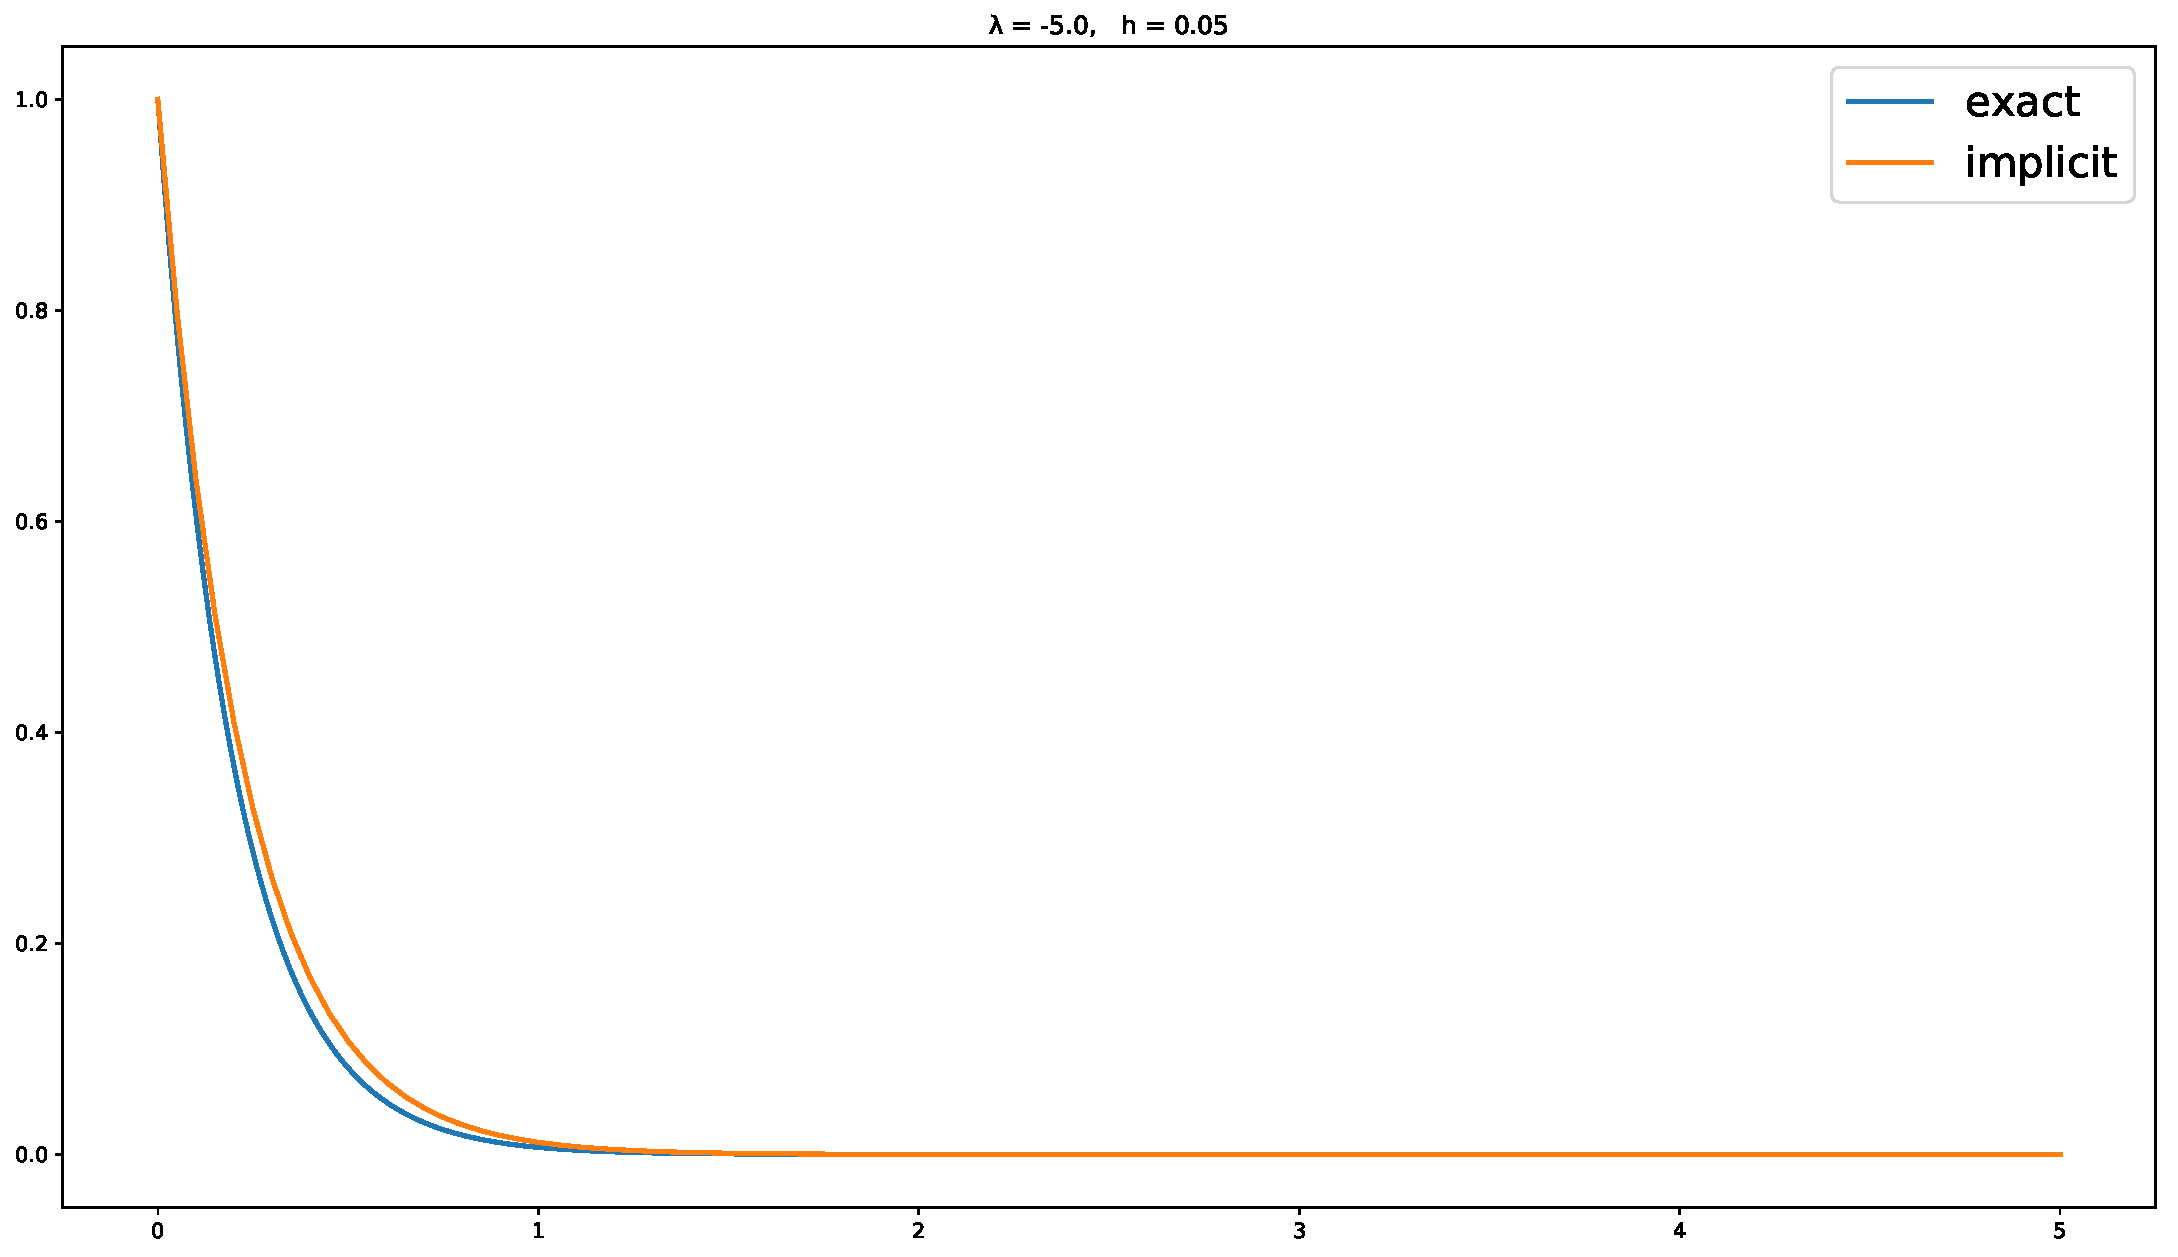
\includegraphics[width=\textwidth]{implicit-euler-lambda--5dot0-h-0dot05} \\
		$\lambda=-5$, $h = 0{,}05$
	\end{minipage}
	\begin{minipage}{0.49\textwidth}
		\centering
		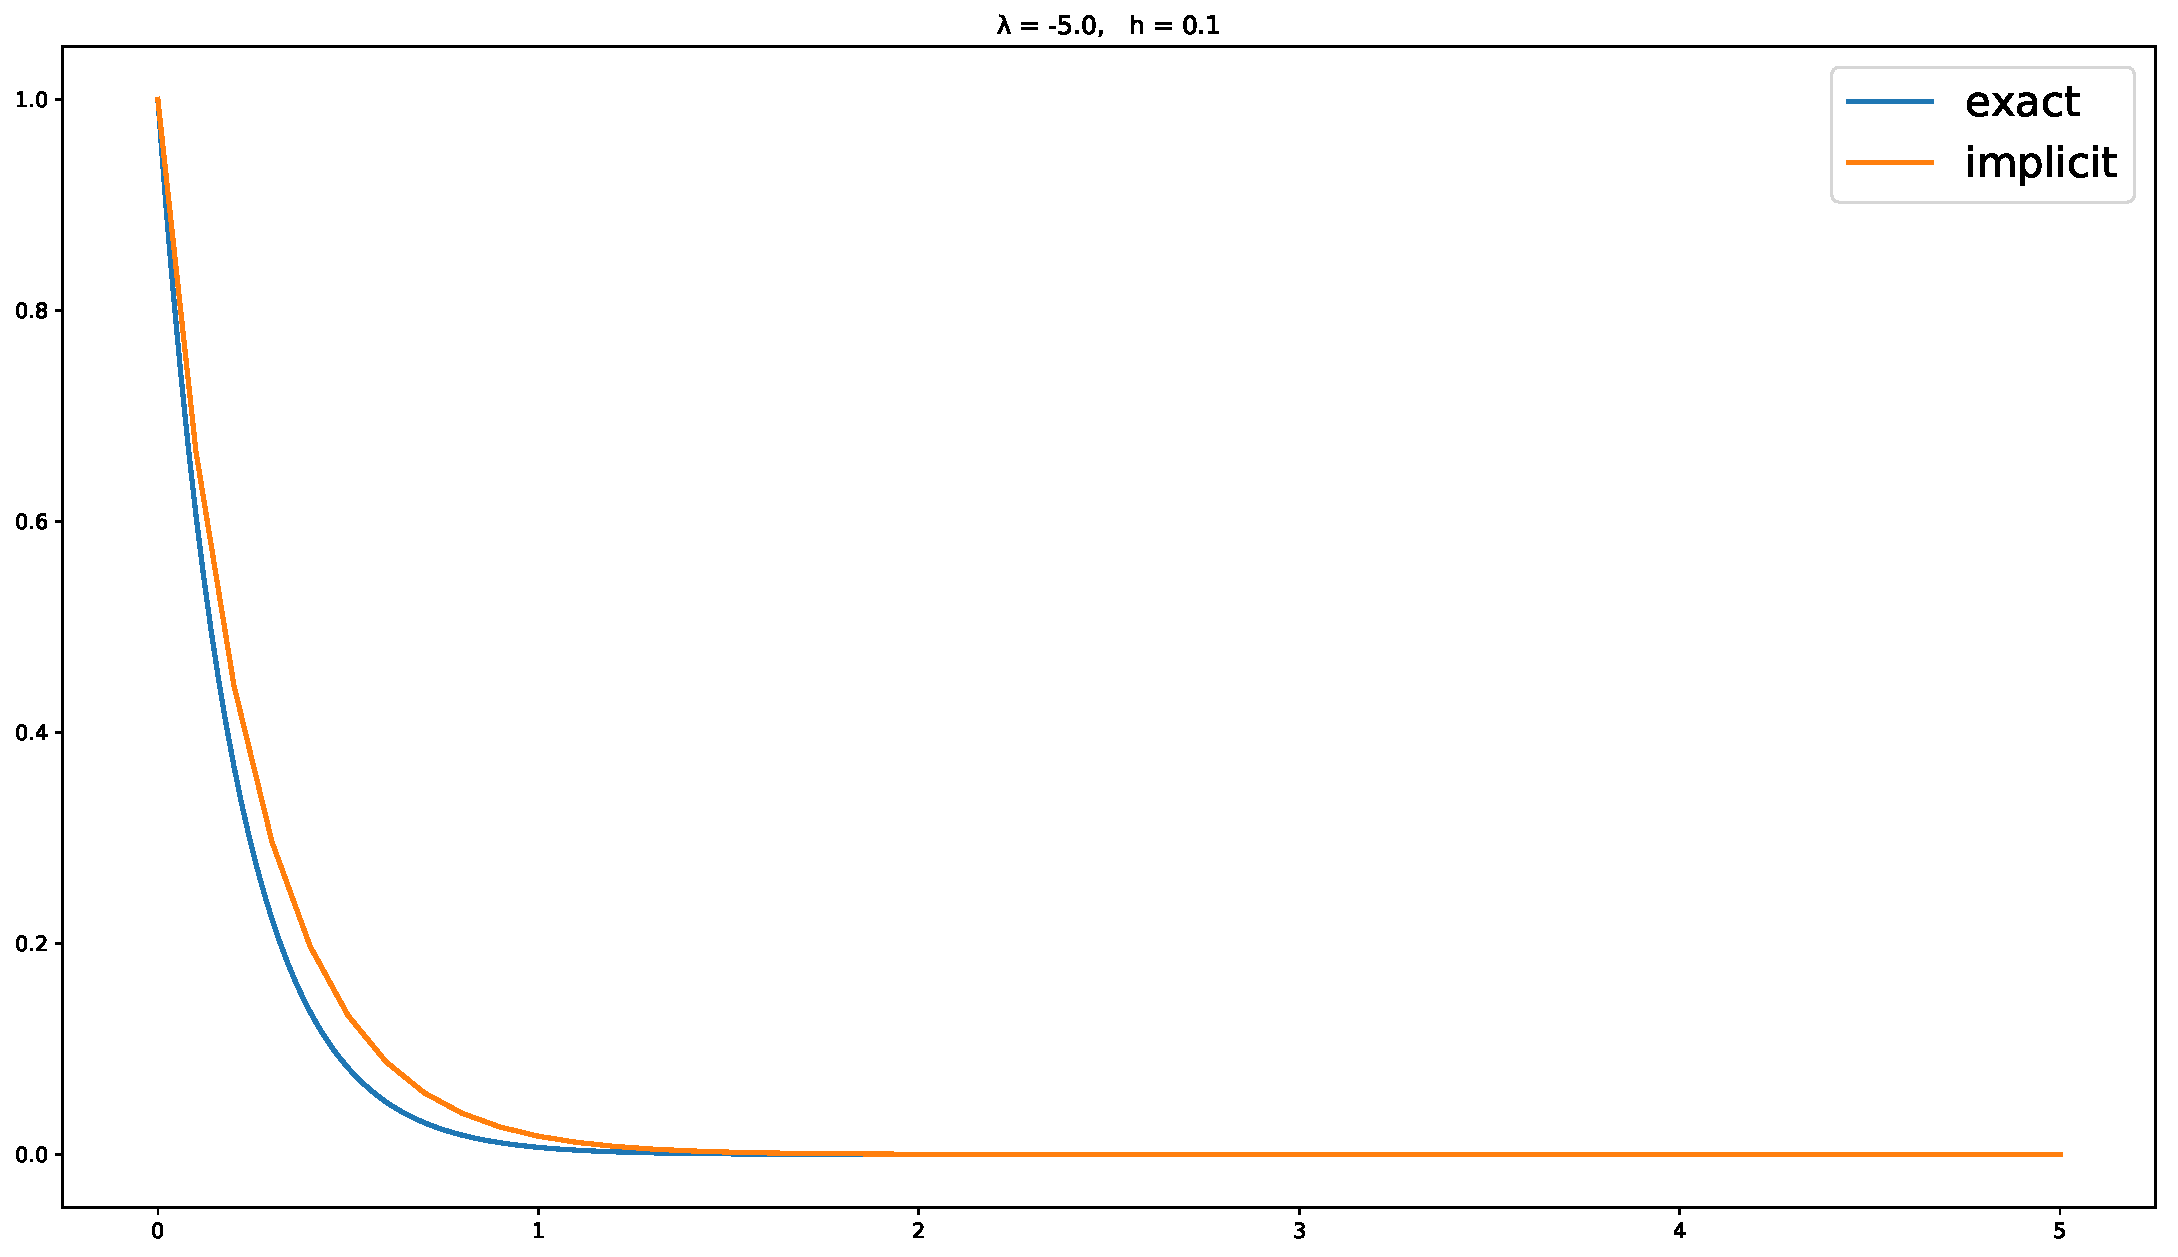
\includegraphics[width=\textwidth]{implicit-euler-lambda--5dot0-h-0dot1} \\
		$\lambda=-5$, $h = 0{,}1$
	\end{minipage}
\end{center}

\begin{center}
	\begin{minipage}{0.49\textwidth}
		\centering
		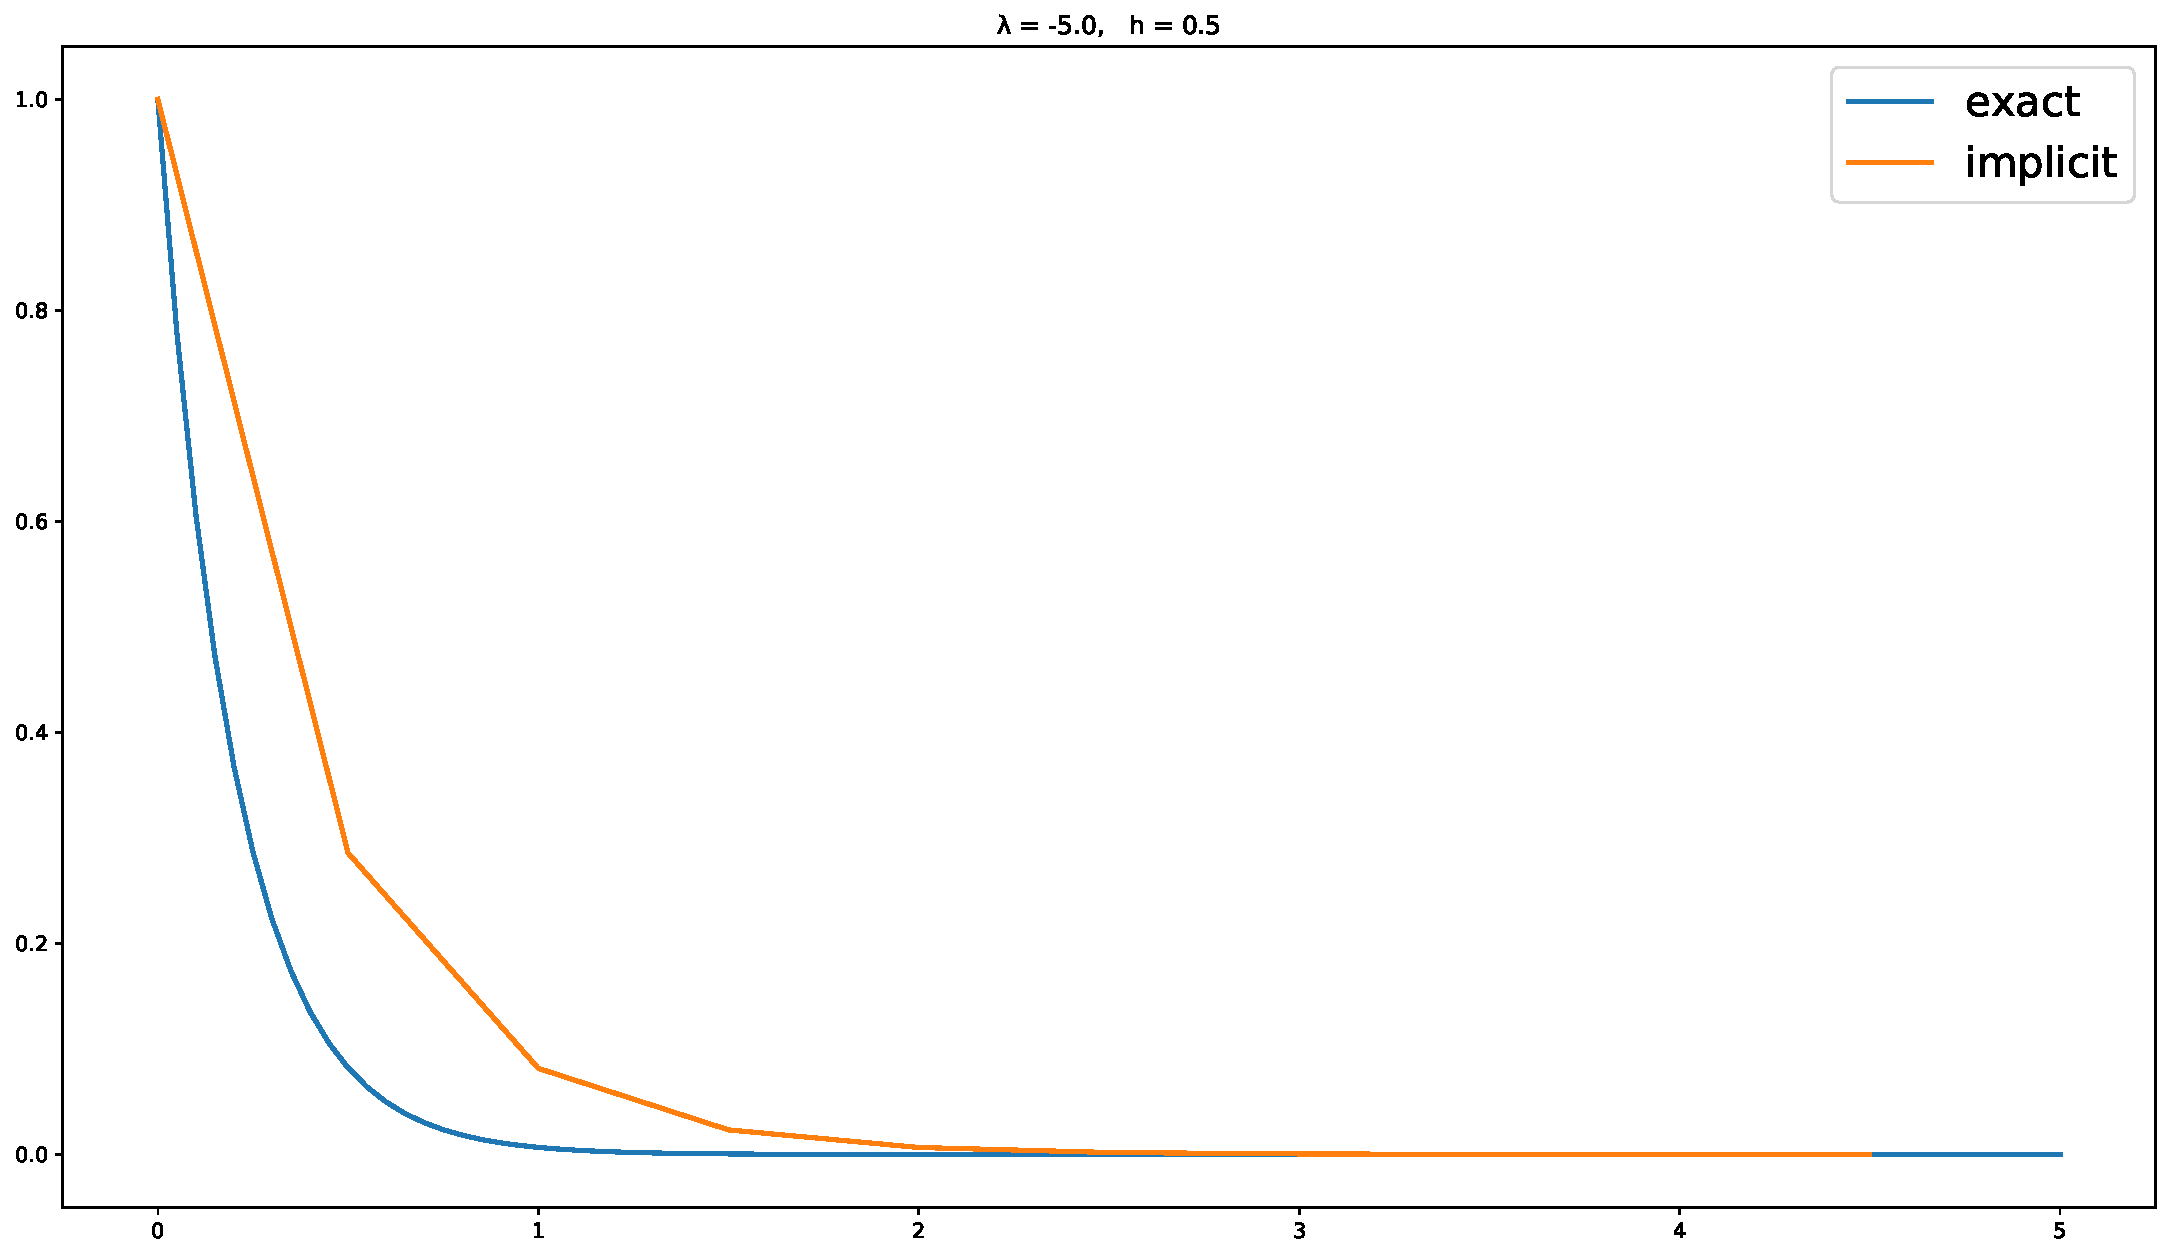
\includegraphics[width=\textwidth]{implicit-euler-lambda--5dot0-h-0dot5} \\
		$\lambda=-5$, $h = 0{,}5$
	\end{minipage}
	\begin{minipage}{0.49\textwidth}
		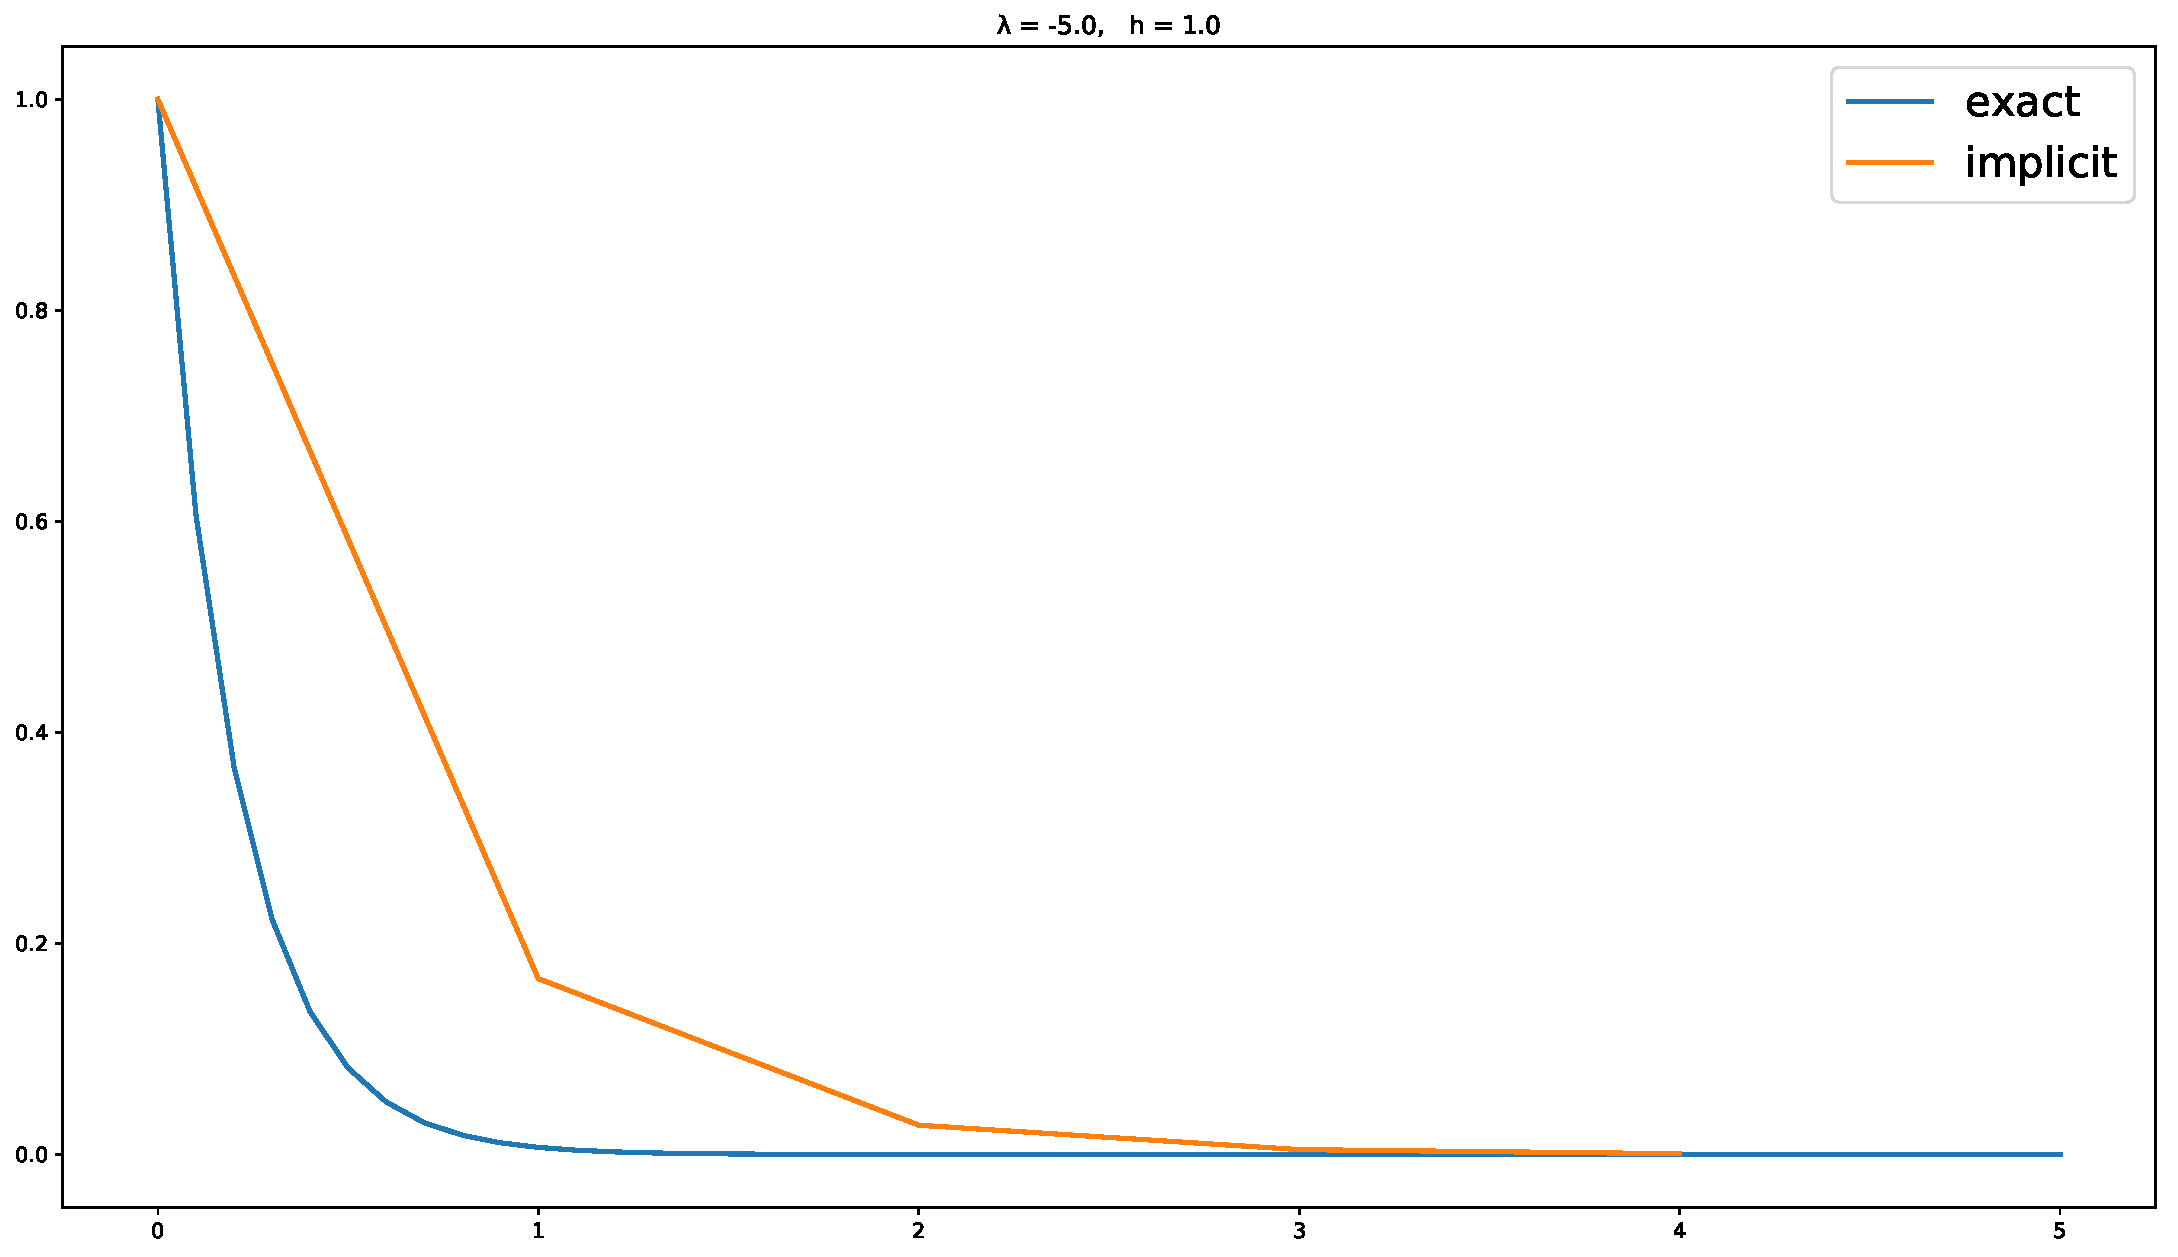
\includegraphics[width=\textwidth]{implicit-euler-lambda--5dot0-h-1dot0} \\	
		$\lambda=-5$, $h = 1{,}0$
	\end{minipage}
\end{center}

Die letzte Rechnung (mit $h=1{,}0$) ist zwar nicht mehr sonderlich präzise,
aber stabil ist sie.

Ist jetzt alles gut?  Nein, denn es steht zu vermuten dass wir für positive $\lambda$ Probleme kriegen.  Und in der Tat, für $\lambda = 1$ sieht das Ergebnis nicht mehr so rosig aus:

\begin{center}
	\begin{minipage}{0.49\textwidth}
		\centering
		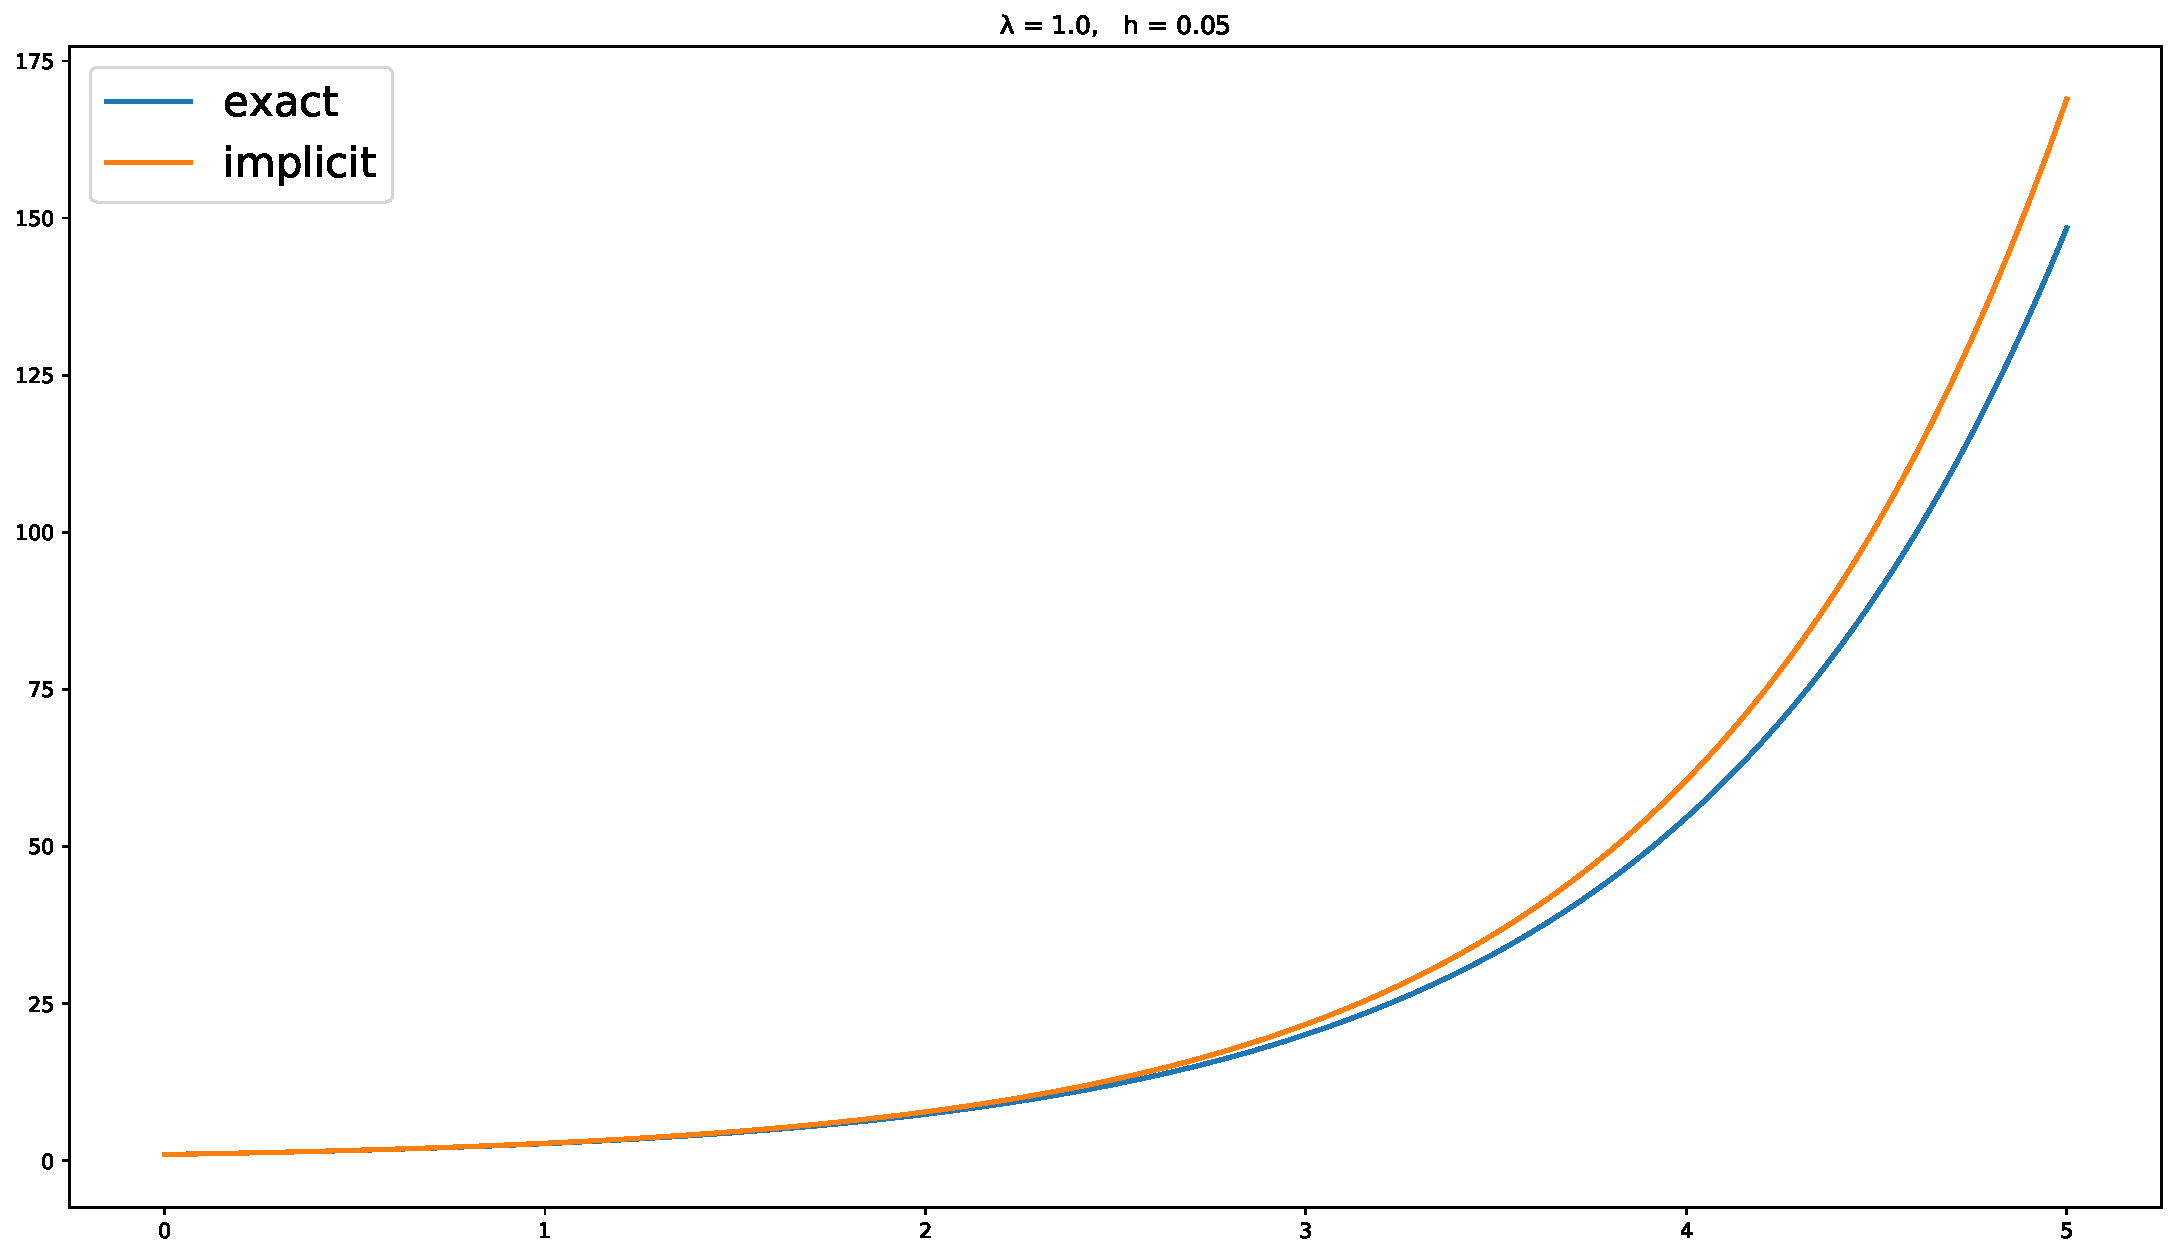
\includegraphics[width=\textwidth]{implicit-euler-lambda-1dot0-h-0dot05} \\
		$\lambda=1$, $h = 0{,}05$
	\end{minipage}
	\begin{minipage}{0.49\textwidth}
		\centering
		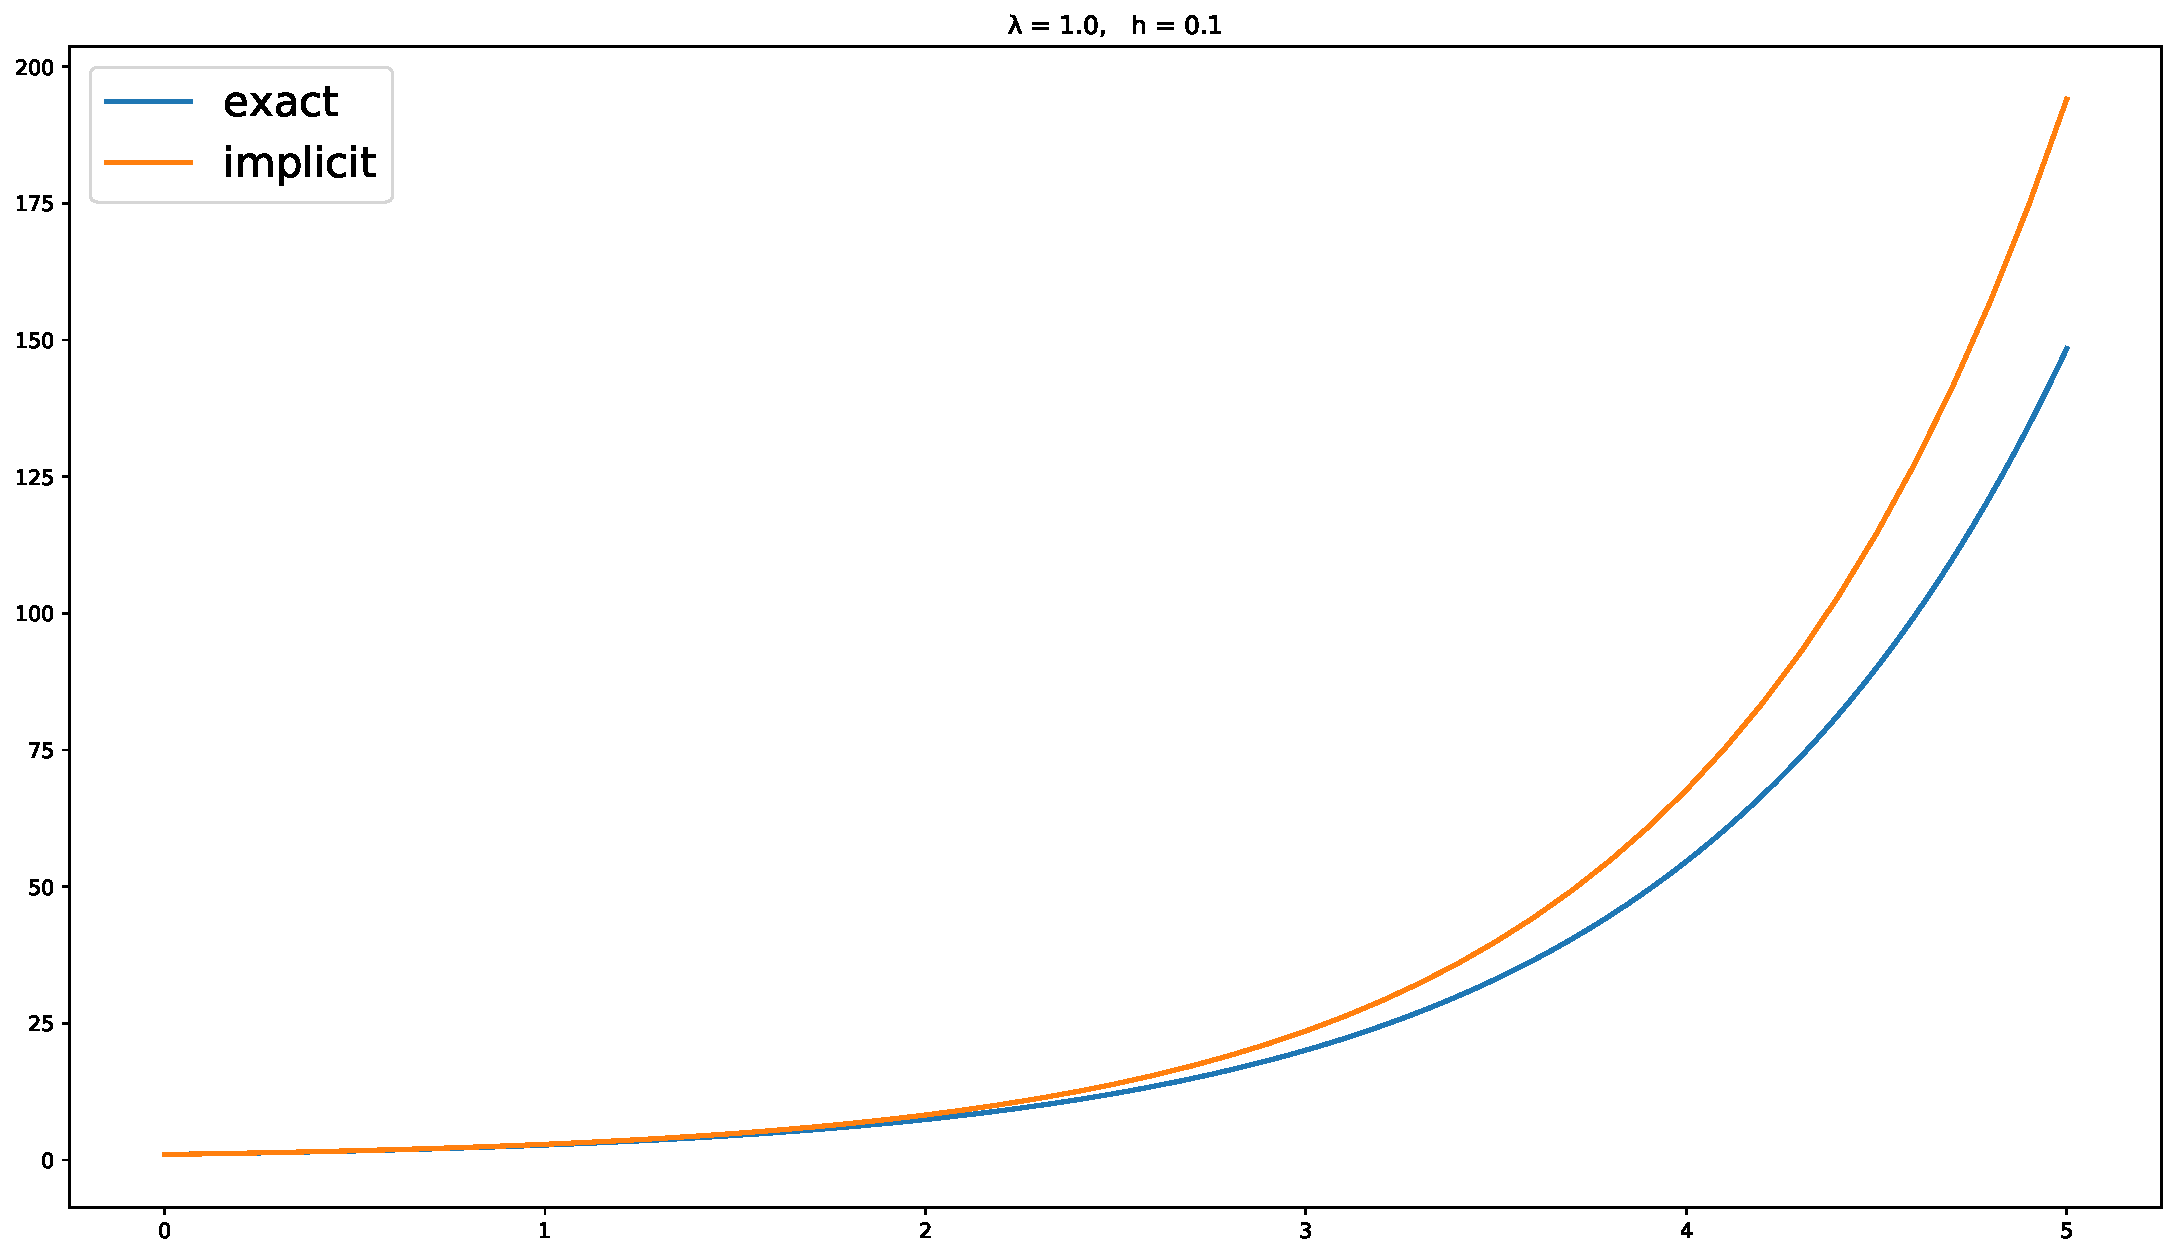
\includegraphics[width=\textwidth]{implicit-euler-lambda-1dot0-h-0dot1} \\
		$\lambda=1$, $h = 0{,}1$
	\end{minipage}
\end{center}
\begin{center}
	\begin{minipage}{0.49\textwidth}
		\centering
		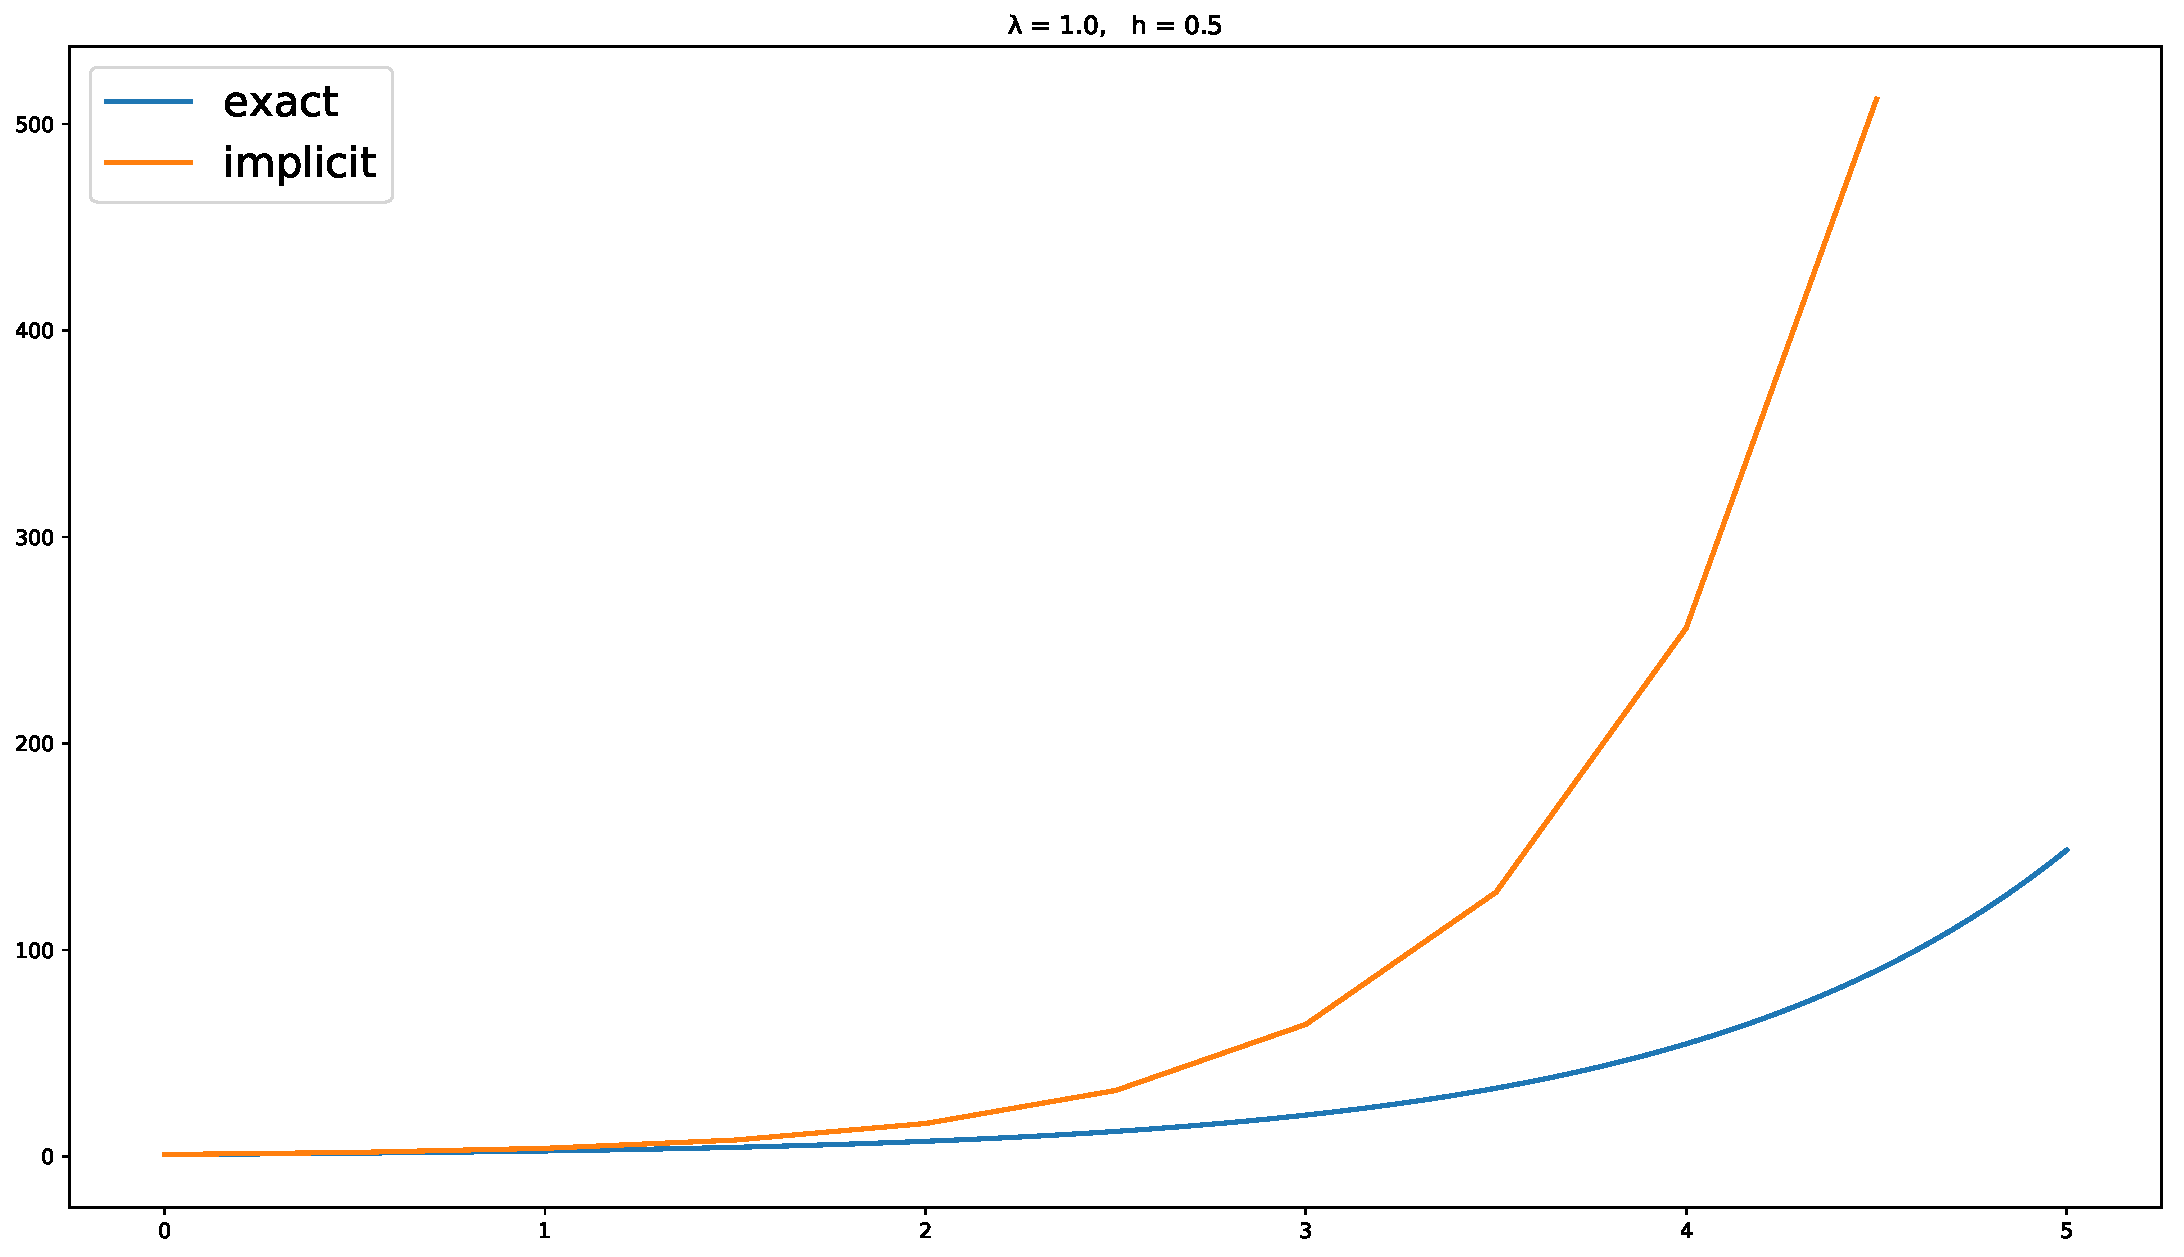
\includegraphics[width=\textwidth]{implicit-euler-lambda-1dot0-h-0dot5} \\
		$\lambda=1$, $h = 0{,}5$
	\end{minipage}
	\begin{minipage}{0.49\textwidth}
		\centering
		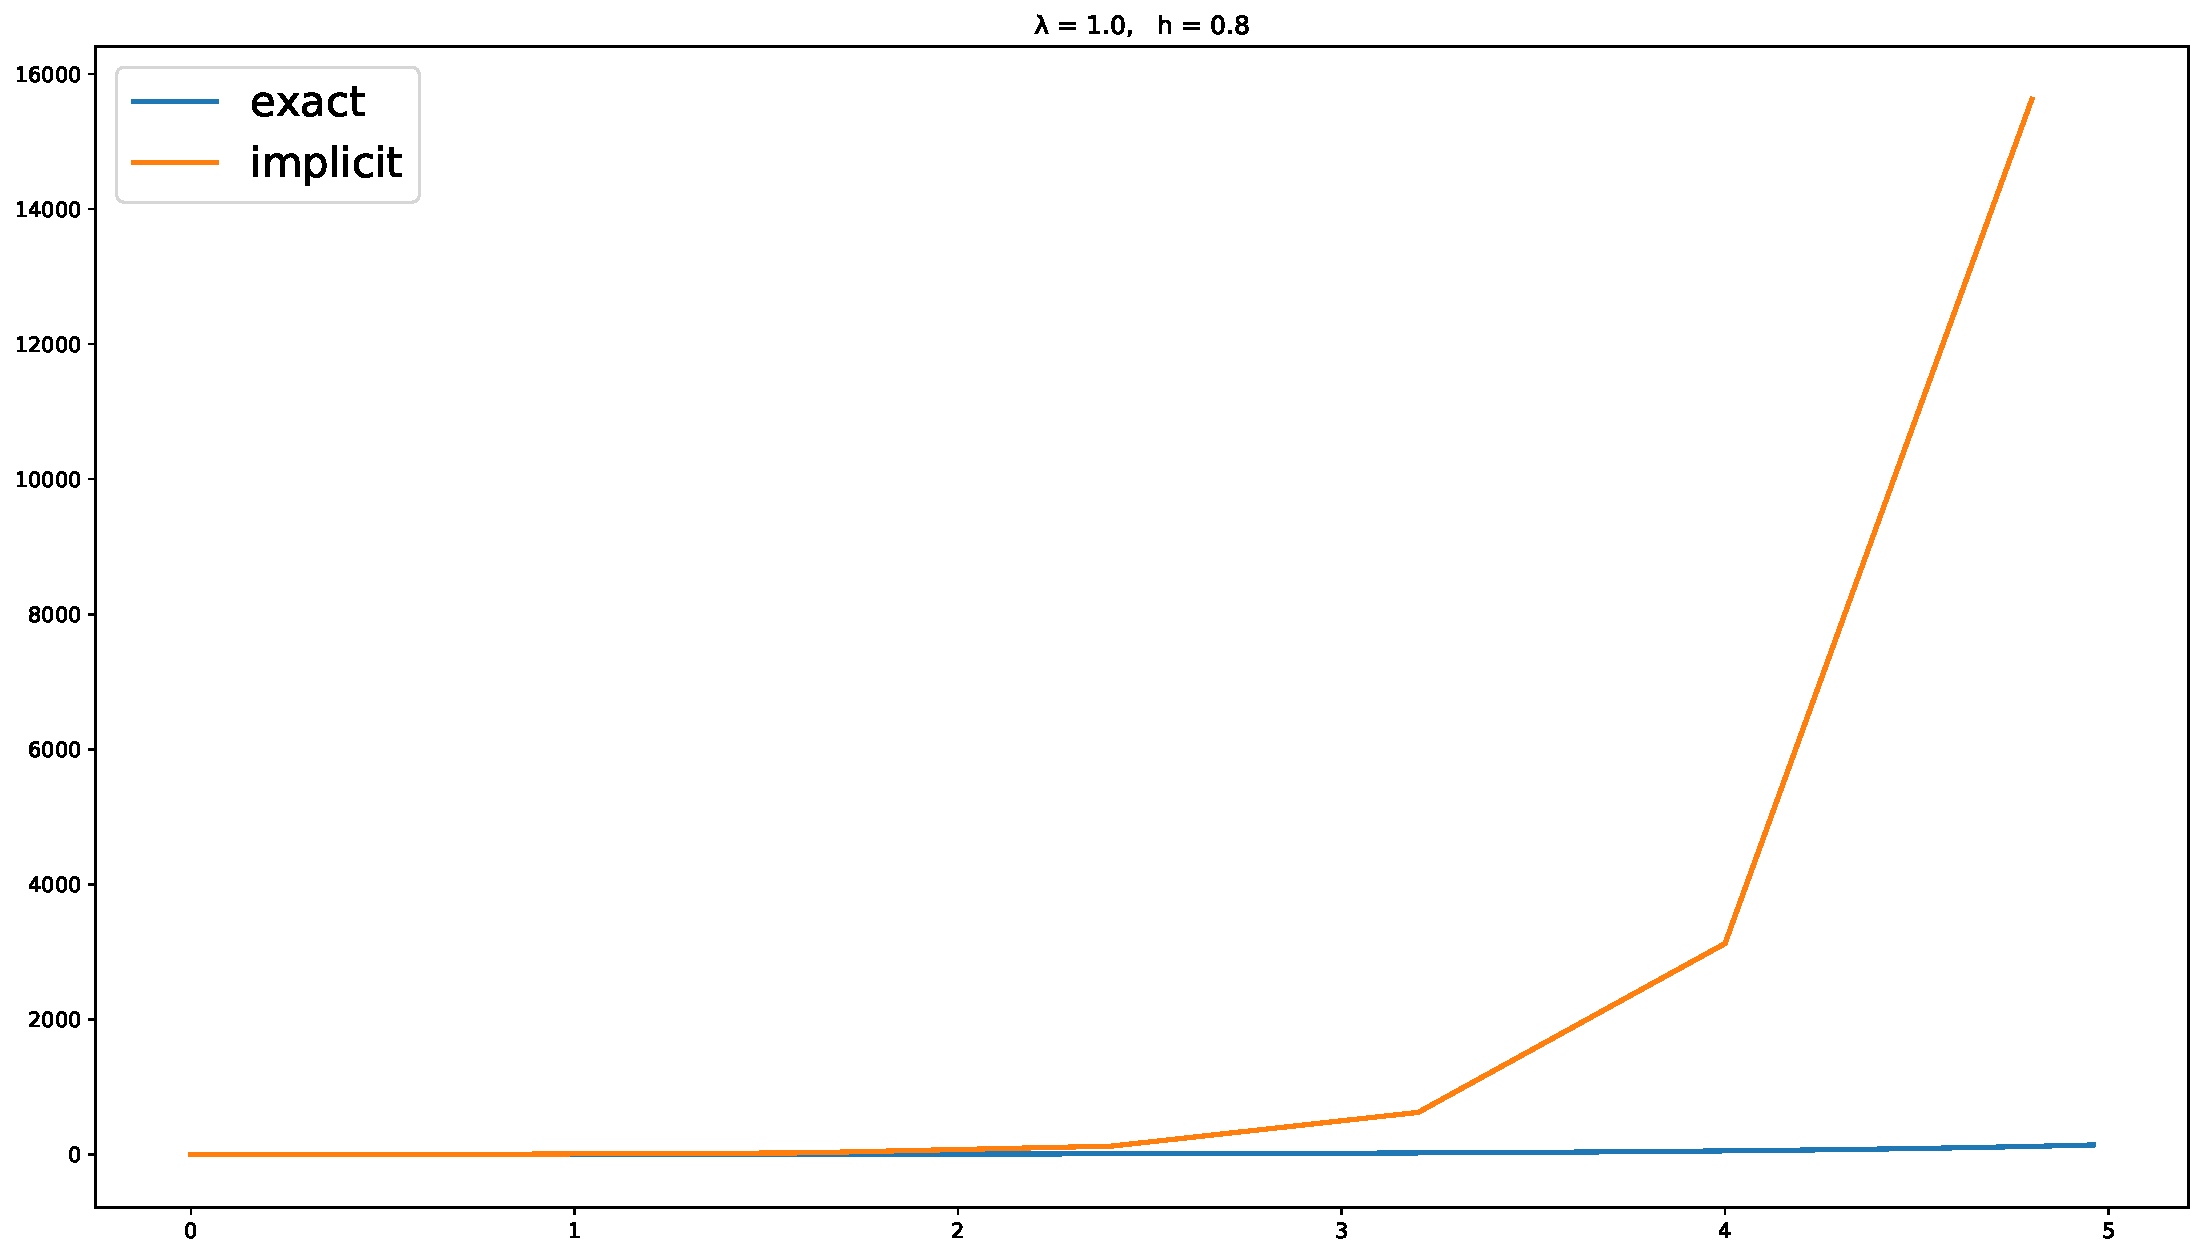
\includegraphics[width=\textwidth]{implicit-euler-lambda-1dot0-h-0dot8} \\
		$\lambda=1$, $h = 0{,}8$
	\end{minipage}
\end{center}

Man beachte hier die wechselnde Skalierung der vertikalen Achse.  Die Zeitschrittweite im letzten Bild ist $0{,}8$ statt wie bisher $1{,}0$, weil der Wert $1{,}0$ im Verfahren zu einer Division durch Null führt.


\section{Stabilität von Einschrittverfahren}

Das explizite Euler-Verfahren wird für die lineare Gleichung
\begin{equation*}
	x' = \lambda x, \qquad x(t_0) = x_0
\end{equation*}
instabil, wenn $\lambda <0$ und der Zeitschritt $\tau$ zu groß ist.

\subsection{Stabilität von linearen, autonomen, homogenen Differentialgleichungen}

Wir verallgemeinern das jetzt und betrachten \textit{lineare}, autonome, homogene Systeme
\begin{equation*}
	x' = Ax \qquad x(0)=x_0 \in \R^d \qquad (A \in \R^{d \times d})
\end{equation*}

\begin{satz}
	Die Lösung dieses AWPs ist
	\begin{equation*}
		x(t)=\exp (tA)x_0
	\end{equation*}
	wobei
	\begin{equation*}
		\exp (tA)\colonequals\sum_{k=0}^{\infty} \frac{(tA)^k}{k!}
	\end{equation*}
	Diese Reihe konvergiert gleichmäßig auf jedem kompakten Zeitintervall.
\end{satz}

Stabilität heißt Störungen im Startwert führen auf beschränkte Störungen in der Lösung (für $t \to \infty$).

Für lineare Gleichungen $x' =Ax$ mit $x(0)=x_0 + \delta_0$ ist die Lösung
\begin{equation*}
	x_{\delta}(t)=\exp (tA) \left(x_0+\delta_0 \right)=\exp (tA)x_0+\exp (tA) \delta_0
\end{equation*}
d.h. die Störung löst das AWP $x' = Ax,\qquad x(0)=\delta_0$.

\begin{lemma}[{{\cite[Lemma~3.20]{deuflhard_bornemann:2008}}}]
	Die Lösung $x$ eines \textit{linearen}, homogenen AWPs ist genau dann stabil, wenn
	\begin{equation*}
		\sup_{t \geq 0} \norm{x(t)} <\infty.
	\end{equation*}
	Sie ist asymptotisch stabil, falls $\norm{x(t)} \xrightarrow[]{t \to \infty} 0$.
\end{lemma}

\begin{bsp}
	$x' =\lambda x$ ist stabil für $\lambda \leq 0$, und asymptotisch stabil für $\lambda <0$.
\end{bsp}

\begin{satz}[{{\cite[Satz~3.23]{deuflhard_bornemann:2008}}}]
	Die Lösung des AWPs
	\begin{equation*}
		x' = Ax\qquad x(0)=x_0\qquad (A\in \C^{d \times d})
	\end{equation*}
	ist genau dann stabil, wenn 
	\begin{itemize}
		\item der Realteil aller Eigenwerte nicht positiv ist und
		\item falls $\lambda$ ein Eigenwert von $A$ mit $\operatorname{Re}(\lambda)=0$, so hat $\lambda$
		die gleiche algebraische und geometrische Vielfachheit.
	\end{itemize}
	Die Lösung ist asymptotisch stabil, falls $\operatorname{Re}(\lambda)<0$ für alle Eigenwerte $\lambda$ von $A$.
\end{satz}


\subsection{Stabilität von linearen autonomen Rekursionen}

\emph{Wunsch}: Die von einem numerischen Verfahren erzeugte Folge $x_k$ soll diese Stabilitätseigenschaften \textit{erben}. Beim expliziten Euler-Verfahren \begin{equation*}
	x_{k+1}=\Psi^{\tau} x_k=x_k+\tau Ax_k=\left(I+\tau A \right)x_k
\end{equation*}
war das nicht der Fall. Beim impliziten Euler-Verfahren
\begin{equation*}
 x_{k+1}=x_k+\tau Ax_{k+1} \implies x_{k+1}=\left(I-\tau A \right)^{-1} x_k
\end{equation*}
jedoch schon!

In Verallgemeinerung betrachten wir nun Verfahren der Form
\begin{equation*}
	x_{k+1}=\Psi^{\tau}x_k=R \left(\tau A \right)x_k
\end{equation*}
mit Polynomen $P$ und $Q$, sodass
\begin{equation*}
	R (\tau A)=\frac{P (\tau A)}{Q (\tau A)}
\end{equation*}

$x_{k+1}$ berechnet sich als Lösung des \textit{linearen} Gleichungssystems
\begin{equation*}
	Q(\tau A)x_{k+1} = Q(\tau A) (\Psi^{\tau} x_k) = P (\tau A) x_k
\end{equation*}
Die rationalen Funktionen werden als Approximationen der Evolution $\Phi^{\tau}=\exp (\tau A)$ verwendet.


Damit $R(A)$ wohldefiniert ist muss $Q(A)$ invertierbar sein -- $Q(A)$ darf also nicht den Eigenwert Null haben.
Wir betrachten nun eine Verallgemeinerung der entsprechenden Bedingung für rationale Funktionen in $\C$:

\begin{lemma}
	Eine rationale Funktion $r \colon z \mapsto \frac{p(z)}{q(z)}$ ist genau dort nicht definiert (bzw. hat genau dort Polstellen), wo $q(z) = 0$ ist.
\end{lemma}

\begin{satz}[{{\cite[Satz~3.42]{deuflhard_bornemann:2008}}}]
	Für eine Matrix $A \in \C^{d \times d}$ ist $R(A)$ genau dann definiert, wenn kein Eigenwert von $A$ Pol von $R$ ist.
\end{satz}


\begin{satz}[{{\cite[Satz~3.33]{deuflhard_bornemann:2008}}}]
	Die lineare Iteration $x_{k+1}=Bx_k$ mit $B \in \C^{d \times d}$ ist genau dann \textit{stabil}, wenn 
	\begin{itemize}
		\item $\left\vert \lambda \right\vert \leq 1$ für alle Eigenwerte $\lambda $ von $B$ und
		\item Falls $\lambda$ Eigenwert von $B$ mit $\left\vert \lambda \right\vert =1$, so hat $\lambda$ gleiche algebraische und geometrische Vielfachheit.
	\end{itemize}
	Die Iteration ist \textit{asymptotisch stabil}, falls $\left\vert \lambda \right\vert <1$ für alle Eigenwerte $\lambda$ von $B$.
\end{satz}


\subsection{Stabilitätsfunktionen}

Wir müssen also die Eigenwerte von
\begin{equation*}
	B = R(\tau A)
\end{equation*}
betrachten. Kann man sie als Funktion von $\tau$ und den Eigenwerte von $A$ berechnen?

Kurioserweise gilt:

\begin{satz}[{{\cite[Satz~3.42, Forts.]{deuflhard_bornemann:2008}}}]
\label{thm:spektrale_aequivarianz}
	Sei $\sigma(A)$ das Spektrum von $A$.  Dann ist
	\begin{equation*}
		\sigma(R(A)) = R(\sigma(A))
	\end{equation*}
\end{satz}
Mit anderen Worten: $\lambda$ ist ein Eigenwert von $A$ genau dann wenn $R(\lambda)$ ein Eigenwert von $R(A)$ ist.

Dabei ist jetzt $R(\lambda)$ die formale rationale Funktion $R$ angewandt auf die komplexe Zahl $\lambda$.

\begin{definition}
	Für ein gegebenes Einschrittverfahren heißt die dazugehörige Funktion $R \colon \C \to \C$ \begriff{Stabilitätsfunktion} des Verfahrens.
\end{definition}

Vererbung von Stabilität heißt damit:  Wenn
\begin{equation*}
	\Re(\lambda) \le 0
	\qquad
	\text{für alle Eigenwerte $\lambda$ von $A$}
\end{equation*}
dann soll auch
\begin{equation*}
	\abs{R(\tau\lambda)} \le 1
	\qquad
	\text{für alle Eigenwerte $\lambda$ von $A$}
\end{equation*}
(plus Zusatzbedingungen für den Fall $\Re \lambda = 0$) gelten.


\begin{defi}
	Die Menge
	\begin{equation*}
		S=\left\lbrace z \in \C \mid \left\vert R(z) \right\vert \leq 1 \right\rbrace
	\end{equation*}
	heißt \begriff{Stabilitätsgebiet} von $R$.
\end{defi}
\begin{bsp}
	Explizites Euler-Verfahren: 
	\begin{equation*}
		x_{k+1}=\underbrace{\left(I+\tau A \right)}_{R \left(\tau A \right)}x_k \Rightarrow R(z)=1+z
	\end{equation*}
	Stabilitätsgebiet: $S=\left\lbrace z \in \C \colon \abs{1+z} \leq 1 \right\rbrace$.
\end{bsp}

Damit ein Verfahren stabil ist muss $\tau \lambda \in S$ für alle $\lambda \in \sigma (A)$ sein.


Im Falle der skalaren Gleichung mit $\lambda \in \R_{< 0}$ und dem Euler-Verfahren führt das auf die Bedingung $\tau \leq \frac{2}{\abs{\lambda}}$.

Für eine graphische Darstellung der Stabilitätsgebiete expliziter Runge-Kutta-Verfahren siehe \cite[Seite~238]{deuflhard_bornemann:2008}. Folgendes Detail sticht ins Auge.

\begin{lemma}[{{\cite[Lemma~6.5]{deuflhard_bornemann:2008}}}]
	Für jede konsistente rationale Approximation von $\exp$ gilt $0 \in \partial S$.
\end{lemma}
Also: 
\begin{itemize}
	\item Die Lösung $x(t)=\exp (tA)x_0$ ist stabil, wenn alle Eigenwerte von $A$ in der linken Halbebene von $\C$ liegen.
	\item Ein numerisches Verfahren $\Psi^{\tau}=R \left(\tau A \right)$ ist stabil, wenn alle Eigenwerte von $\tau A$ in $S$ liegen (plus Zusatzbedingungen am Rand von $S$).
\end{itemize}

Folgende Eigenschaft ist deshalb wünschenswert:

\begin{defi}
	Ein Einschrittverfahren heißt \begriff{A-stabil}, falls sein Stabilitätsgebiet die negative komplexe Halbebene enthält.
\end{defi}

In diesem Fall gibt es keine Schrittweitenbeschränkung!

Explizite Verfahren können aber nicht A-stabil sein.

\begin{lemma}
	Die Flüsse aller expliziten Runge-Kutta-Verfahren (für lineare Gleichungen) sind Polynome in $\tau A$, also $\Psi^{\tau} x=P (\tau A)x$.
\end{lemma}
\begin{proof}
	Wir zeigen dass für jedes $i\le s$ der Ausdruck $\tau k_i$ ein formales Polynom in $\tau A$ ist. Dann folgt die Behauptung aus
	\begin{equation*}
		\Psi^{t+\tau,t}x 
		= x + \tau \sum_{i=1}^s b_i k_i
		= (\tau A)^0 x + \sum_{i=1}^s b_i \tau k_i.
	\end{equation*}
	Beweis mit vollständiger Induktion: Betrachte ein RK-Verfahren für $x' = Ax$:
	\begin{equation*}
		k_i 
		= f(t + c_i \tau, x + \tau \sum_{j=1}^{i-1} a_{ij} k_j)
		= A\Big[ x + \tau \sum_{j=1}^{i-1} a_{ij} k_j \Big]
	\end{equation*}
	\begin{itemize}
		\item $\tau k_1 = \tau Ax$ ist Polynom in $\tau A$.
		\item Seien $\tau k_j$ Polynome für alle $j<1$.  Dann ist
		\begin{equation*}
			\tau k_i = \tau Ax + \tau A \sum_{j+1}^{i-1} a_{ij} \tau k_j
		\end{equation*}
		ein Polynom in $\tau A$.
	\end{itemize}
\end{proof}


\begin{lemma}[{{\cite[Lemma~6.11]{deuflhard_bornemann:2008}}}]
	Das Stabilitätsgebiet von Polynomen ist kompakt.
\end{lemma}
\begin{proof}
	Für jedes Polynom $P$ vom Grad $\geq 1$ gilt $\left\vert P(z) \right\vert \xrightarrow[]{z \to \infty} \infty$. Also ist $S$ beschränkt.
\end{proof}

Implizite Verfahren können A-stabil sein: z.B. das implizite Euler-Verfahren: \begin{equation*}
	R(z)=\frac{1}{1-z}
\end{equation*}
mit dem Stabilitätsgebiet: $S=\{ z \in \C \mid \abs{1-z} \geq 1 \} \supset \C$.

\medskip

Das Ziel für die Zukunft lautet jetzt, A-stabile Verfahren hoher Ordnung zu konstruieren.

\section{Implizite Runge--Kutta-Verfahren}

Wir betrachten jetzt wieder allgemeine nichtlineare, nicht-autonome Anfangswertprobleme
\begin{equation*}
	x' = f(t,x) \qquad x(t_0) = x_0
\end{equation*}
Wie können wir stabile Verfahren hoher Konsistenzordnung konstruieren?

\begin{defi}[Butcher 1964]
	Unter einem \begriff{allgemeinen Runge-Kutta-Verfahren} (kurz: RK-Verfahren) verstehen wir ein Verfahren der Form
	\begin{align*}
		k_i &= f\Big(t + c_i \tau, x + \tau \sum_{j=1}^s a_{ij} k_j\Big), \qquad i=1,\dots,s, \tag{i}\\
		\Psi^{t + \tau,t} x &= x + \tau \sum_{j=1}^s b_j k_j \tag{ii}
	\end{align*}
\end{defi}

Im Unterschied zu expliziten RK-Verfahren geht die Summe in (i) über alle $s$ Stufen, nicht nur über die ersten $i-1$.

Man fasst die Koeffizienten wieder in zwei Vektoren $b,c \in \R^s$ und eine Matrix $\mathcal A \in \R^{s\times s}$
zusammen. Darstellung der Koeffizienten wieder im Butcher-Schema:
\begin{center}
	\begin{tabular}{c|c}
		$c$ & $\mathcal A$ \\ \hline
		& $b^T$
	\end{tabular}
\end{center}

\begin{bsp}[Implizites Euler-Verfahrens]~\\
	\begin{center}
		\begin{tabular}{c|c}
			$1$ & $1$ \\ \hline
			& $1$
		\end{tabular}
	\end{center}
\end{bsp}

Ein Verfahren ist explizit, wenn $\mathcal A$ eine strikte untere Dreiecksmatrix ist. Ansonsten muss in jedem Schritt ein nichtlineares Gleichungssystem gelöst werden.

\emph{Frage:} Unter welchen Bedingungen ist dieses Gleichungssystem eindeutig lösbar (für hinreichend kleine $\tau$?) Nur dann kann ja von einem wohldefinierten Zeitintegrationsverfahren gesprochen werden.

Um diese Frage zu klären schreiben wir das Verfahren zunächst in der sogenannten
\emph{symmetrischen Form} auf. Definiere
\begin{equation*}
	g_i = x + \tau \sum_{j=1}^s a_{ij} k_j,
	\qquad
	i=1,\dots,s
\end{equation*}
Dann gilt
\begin{align*}
	g_i
	& = x + \tau \sum_{j=1}^s a_{ij} f(t + c_j \tau, g_j)
	\qquad i=1,\dots,s \\
	%
	\Psi^{t+\tau,t} x
	& = x + \tau \sum_{j=1}^s b_j f(t + c_j \tau, g_j)
\end{align*}


\begin{satz}[{{\cite[Satz~6.28]{deuflhard_bornemann:2008}}}]
\label{eq:wellposedness_of_implicit_rk_methods}
	Die Abbildung $f \in C(\Omega, \R^d)$ sei auf $\Omega \subset \R \times \R^d$ bezüglich $x$ lokal Lipschitz-stetig. Für ein implizites RK-Verfahren gibt es zu jedem $(x,t) \in \Omega$ ein $\tau_\ast > 0$, und \textit{eindeutige} stetige Funktionen
	\begin{equation*}
		g_i \colon (-\tau_\ast, \tau_\ast) \to \R^d \qquad (i=1,\dots,s)
	\end{equation*} 
	so dass:
	\begin{enumerate}
		\item $g_i(0) = x$ für $i=1,\dots, s$
		\item Für $\abs{\tau} < \tau_\ast$ genügen die Vektoren $g_i(\tau)$, $i=1,\dots,s$, den Bestimmungsgleichungen des impliziten RK-Verfahrens.
	\end{enumerate}
\end{satz} 

Für den Beweis brauchen wir einen besonderen, parameterabhängigen Fixpunktsatz.
Den Beweis dazu findet man bei~\cite[Satz~10.1.1]{dieudonne:1960}.

\begin{satz}
\label{thm:parameter_fixed_point}
	Es seien $E_1$ und $E_2$ zwei Banach-Räume. $U$ und $V$ seien offene Kugeln in $E_1$ (bzw. $E_2$) jeweils um $0$; der Radius von $V$ sei $\beta$.
	Sei $F$ eine stetige Abbildung von $U \times V$ nach $E_2$, so dass
	$\norm{F(\tau,y_1) - F(\tau,y_2)} \le \theta \cdot \norm{y_1 - y_2}$
	für $\tau \in U$, $y_1, y_2 \in V$ und $\theta$ eine Konstante mit $0 \le \theta < 1$.
	Falls $\norm{F(\tau,0)} < \beta (1-\theta)$ für alle $\tau \in U$, existiert
	dann eine eindeutige Abbildung $g : U \to V$ so dass
	\begin{equation*}
		g(\tau) = F(\tau,g(\tau))
	\end{equation*}
	für alle $\tau \in U$, und $g$ ist stetig in $U$.
\end{satz}


\begin{proof}[Satz~\ref{eq:wellposedness_of_implicit_rk_methods}]
	\begin{itemize}
		\item Sei $(t_0,x_0) \in \Omega$ fest gewählt.
		\item $f$ ist lokal Lipschitz-stetig bezüglich $x$. D.h. es gibt Parameter $\tau_1, \rho, L > 0$ so dass $\abs{f(t,x) - f(t,\bar x)} < L \abs{x - \bar x}$ für alle $(t,x), (t, \bar x) \in (t_0 - \tau_1, t_0 + \tau_1) \times B_\rho (x_0) \subset \Omega$.
		\item Weiterhin gilt $\abs{f(t,x_0)} < M$ für alle $t \in (t_0 - \tau_1, t_0 + \tau_1)$ (zur Not wird dafür $\tau_1$ verkleinert).
		\item Wir wählen jetzt ein $0 < \theta < 1$ (Das wird das $\theta$ aus dem Satz von Dieudonn\'e).
		%
		\item Schreibe das RK-System als parameterabhängige Fixpunktgleichung $g(\tau) = F(\tau,g(\tau))$ mit 
		\begin{align*}
			g &\colonequals (g_1, \dots, g_s)^T, \\
			F(\tau,g) &\colonequals \big( F_1(\tau, g), \dots, F_s(\tau,g) \big)^T, \\
			F_i(\tau,g) &= x_0 + \tau \sum_{j=1}^{s} a_{ij} f(t_0 + c_j \tau, g_j), \qquad i = 1,\dots s.
		\end{align*}
		\item $g$ ist aus $E_2 = \R^{s \cdot d}$. Wähle dort die Norm $ \norm{g} = \max_{1 \le i \le s} \abs{g_i}$.
		\item Notation: $g_\ast \colonequals (x_0, \dots, x_0) \in \R^{s\cdot d}$.
		\item Jetzt definieren wir die Kugeln in $E_1 = \R$ und $E_2 = \R^{s\cdot d}$
		\begin{equation*}
			U = (-\tau_\ast, \tau_\ast), \qquad V = \{ g \in \R^{s\cdot d} \mid \norm{g - g_\ast} < \rho \}
		\end{equation*}		
		\item Damit ist  $F: U \times V \rightarrow \R^{s\cdot d}$  wohldefiniert und stetig.
		\item Wir zeigen als nächstes die Lipschitz-Stetigkeit von $F$ im zweiten Argument: 
		Für alle $(\tau,g), (\tau, \bar g) \in U \times V$ gilt
		\begin{align*}
			\norm{F(\tau,g) - F(\tau, \bar g)} & = 
			\norm{(F_1(\tau,g) - F_1(\tau, \bar g), \dots, F_s(\tau, g) - F_s(\tau, \bar g))^T} \\
			&= \max_{1\le i \le s} \abs{F_i(\tau,g) - F_i(\tau, \bar g)} \\
			%
			&= \max_{1\le i \le s} \Big| x_0 + \tau \sum_{j=1}^s a_{ij} f(t_0 + c_j \tau, g_j ) - x_0
				- \tau \sum_{j=1}^s a_{ij} f(t_0 + c_j \tau, \bar g_j ) \Big| \\
			%
			&\le \tau \max_{1\le i \le s} \sum_{j=1}^s \Big [\abs{a_{ij}}
			\cdot \big| f(t_0 + c_j \tau, g_j ) -  f(t_0 + c_j \tau, \bar g_j ) \big| \Big] \\
			%
			&\le \tau \underbrace{\max_{1\le i \le s} \sum_{j=1}^s \abs{a_{ij}}}_{= \norm{\mathcal A}_\infty}
			\cdot \max_{1 \le j \le s} \big| f(t_0 + c_j \tau, g_j ) -  f(t_0 + c_j \tau, \bar g_j ) \big| \\
			%
			& \le \tau_\ast \norm{\mathcal A}_\infty  \max_{1\le j \le s}  \Big| f(t_0 + c_j \tau, g_j) - f(t_0 + c_j \tau, \bar g_j)\Big|.
			\end{align*} 
		\item Da $f$ lokal Lipschitz-stetig im zweiten Argument ist, gilt
		\begin{align*}
			\norm{ F(\tau,g) - F(\tau, \bar g)} &\le \tau_\ast \norm{\mathcal A}_\infty L \max_{1\le j \le s}  \abs{g_j - \bar g_j} \\
			&= \tau_\ast \norm{\mathcal A}_\infty L \norm{g - \bar g} \\
			& \le \theta \norm{g - \bar g}
		\end{align*} 
		wenn $\tau_\ast \le \frac{\theta}{L\norm{\mathcal{A}}_\infty}$.
		\item Ähnlich zeigt man
		\begin{align*}
			\norm{F(\tau, g_\ast) - g_\ast}
			& =
			\norm{F(\tau, g_\ast) - F(0,g_\ast)} \\
			%
			& = \max_{1 \le i \le s} \Big| x_0 + \tau \sum_{j=1}^s a_{ij} f(t_0 + c_j \tau, x_0) - x_0 -0\Big| \\
			%
			& =
			\max_{1 \le i \le s} \Big| \tau \sum_{j=1}^s a_{ij} f(t_0 + c_j \tau, x_0) \Big| \\
			& \le
			\tau_\ast \norm{\mathcal{A}}_\infty \max_{1 \le j \le s} \abs{f(t_0 + c_j \tau,x_0)} \\
			& <
			\tau_\ast \norm{\mathcal{A}}_\infty M \\
			%
			& \le \rho(1 - \theta),
		\end{align*}
		falls $\tau_\ast \le \frac{\rho(1-\theta)}{\norm{\mathcal{A}}_\infty M}$.

		(Der Fixpunktsatz fordert $\norm{F(\tau, 0) - 0} \le \rho(1 - \theta)$,
		weil dort die Kugeln um $0$ zentriert sind, und nicht wie hier um $g_\ast$.)
		\end{itemize}
	Wende jetzt den parameterabhängigen Fixpunktsatz~\ref{thm:parameter_fixed_point} an. Er liefert
	\begin{itemize}
		\item Es existieren eindeutige $g(\tau) \in V$ für alle $\tau \in U = (-\tau_\ast,\tau_\ast)$, so dass
		$$ g(\tau) = F\big(\tau, g(\tau)\big). $$
		\item $g(\tau)$ ist stetig, insbesondere ist $g(0) = g_\ast$.
	\end{itemize}
\end{proof}

Implizite RK-Verfahren sind also für kleine $\tau$ wohldefiniert.
Wie sieht es mit Konsistenz und Stabilität aus?

\textbf{Erinnerung:} Konsistenztheorie für explizite RK-Verfahren
\begin{itemize}
	\item Entwickle $\Phi$ und $\Psi$ als Taylorreihen
	\item Wähle die Koeffizienten $b,c, \mathcal A$ so, dass möglichst viele Terme aus der Taylorreihe von $\Phi$  reproduziert werden.
\end{itemize}

Im Prinzip funktioniert das für implizite Verfahren genauso. Jedoch ist alles etwas komplizierter: Es müssen mehr Koeffizienten bestimmt werden; aber auch alles etwas einfacher: Für eine gegebene Ordnung $p$ erhält man die gleiche Anzahl von Bestimmungsgleichungen wie im expliziten Fall \cite[Satz~4.24]{deuflhard_bornemann:2008}. Man hat aber mehr Freiheitsgrade, um diese zu erfüllen.

\begin{satz}
	Unter den Bedingungen des obigen Satzes gilt:
	\begin{itemize}
		\item Die Evolution $\Psi$ ist genau dann konsistent, wenn
		\begin{equation*}
			\sum_{i=1}^s b_i = 1
		\end{equation*}
		\item Ist $f \in C^p(\Omega, \R^d)$, so ist auch $\Psi^{t+\tau, t} x$ in $\tau$ $p$-fach differenzierbar.
	\end{itemize}
\end{satz}

Wie für explizite Verfahren zeigt man: Ein implizites Verfahren ist genau dann invariant unter Autonomisierung, wenn es konsistent ist und
\begin{equation*}
	c_i = \sum_{j=1}^{s} a_{ij} \qquad \text{für } i=1,\dots, s
\end{equation*}
gilt. 

Welche Ordnung kann man maximal erzielen? $\to$ Dafür braucht man die Stabilitätsfunktion.

\begin{lemma} 
	Die Stabilitätsfunktion $R$ eines $s$-stufigen RK-Verfahrens $(b,\mathcal A)$ ist durch
	\begin{equation*}
		R(z) = 1 + zb^T (I - z\mathcal A)^{-1} (1,\dots,1)^T
	\end{equation*}
	gegeben. Die Funktion $R$ kann in eindeutiger Weise als 
	\begin{equation*}
		R(z) = \frac{P(z)}{Q(z)}
	\end{equation*}
	dargestellt werden, wobei $P,Q$ teilerfremde Polynome höchstens $s$-ten Grades mit $P(0) = Q(0) = 1$ sind.
\end{lemma}
\begin{proof}
	Übung.
\end{proof}

\textbf{Erinnerung:} Ein $s$-stufiges explizites RK-Verfahren hat höchstens die Konsistenzordnung $p \le s$.
\begin{lemma}
	Ein $s$-stufiges implizites RK-Verfahren besitze für alle $f \in C^\infty(\Omega, \R^d)$ die Konsistenzordnung $p \in \N$. Dann gilt $ p \le 2s$.
\end{lemma}
\begin{proof}
	\begin{itemize}
		\item Betrachte das AWP $x' = x$, $x(0) =1$ mit Lösung $x(\tau) = e^{\tau}$ und RK-Approximation $\Psi^\tau$.
		\item Das Verfahren ist konsistent mit Konsistenzordnung $p$, also gilt
		\begin{equation*}
			\Psi^\tau 1 - \Phi^\tau 1 = R(\tau) - e^\tau = \mathcal O(\tau^{p+1})
		\end{equation*}
		\item $R = \frac{P}{Q}$ ist Quotient zweier Polynome mit Ordnung jeweils $\le s$. Es folgt $p \le \deg P + \deg Q \le 2s$.
	\end{itemize}
	Warum? Angenommen es gäbe Polynome $P, Q$ mit $\deg P \le k$ und $\deg Q \le j$ sowie $k+j < p$. Das hieße $\frac{P(z)}{Q(z)} - e^z = \mathcal O(z^{k+j+2})$. Multiplikation mit $Q(z)$liefert dann $P(z) - Q(z) e^z =  \mathcal O(z^{k+j+2})$. Daraus folgt $P = Q = 0$ ein Widerspruch!
	(Beweis: Übung. \cite[Lemma~6.4]{deuflhard_bornemann:2008})
\end{proof}


\section{Kollokationsverfahren}

Wie konstruiert man jetzt konkrete RK-Verfahren?
Die folgende Idee ist unabhängig von den RK-Verfahren entwickelt worden.
Dass man dadurch implizite RK-Verfahren erhält wurde erst in den 1970ern entdeckt.

Betrachte 
\begin{equation*}
	x' = f(t,x)
\end{equation*}
Seien $(t,x) \in \Omega$ und eine Schrittweite $\tau$ gegeben. Gesucht ist nun ein Schritt einer diskreten Evolution $\Psi^{t + \tau, t} x$.
\textbf{Idee:}

\begin{idea}
	\begin{itemize}
		\item Wähle $s$ Stützstellen im Intervall $(t, t+ \tau)$
		\begin{equation*}
			t + c_i \tau \qquad 0 \le c_1 < c_2 < \dots < c_s \le 1 
		\end{equation*}
		\item Konstruiere ein Polynom $u \in P_s^d$, das 
		\begin{enumerate}
			\item \label{enum:colloq_AW} den Anfangswert $u(t) = x$ erfüllt und
			\item \label{enum:colloq_DGL} die Differentialgleichung an den Stützstellen erfüllt
			\begin{equation*}
				u'(t + c_i \tau) = f(t + c_i \tau, u(t+c_i \tau)) \tag{$i=1,\dots, s$}
			\end{equation*}
			\item \label{enum:colloq_Disc} Setze
			\begin{equation*}
				\Psi^{t+\tau,t} x \colonequals u(t+\tau)
			\end{equation*} 
			\todoannot{\baselineskip}{Ein Bild!}
		\end{enumerate}
		Diese Bedingungen nennen wir \begriff{Kollokationsbedingungen}.
	\end{itemize}
\end{idea}

Einziger Parameter des Verfahrens sind die Stützstellen $c_1, \dots, c_s$. Wir haben $s+1$ Bedingungen an ein Polynom $s$-ten Grades. Wir \textit{vermuten}, dass ein eindeutiges $u$ existiert (zumindest für kleine $\tau$). Klar ist das nicht, denn die Gleichungen für $u$ sind nichtlinear!

Einfacher Ausweg: Wir interpretieren das Verfahren als implizites RK-Verfahren. Dann liefert Satz \ref{eq:wellposedness_of_implicit_rk_methods} Existenz und Eindeutigkeit.
\begin{itemize}
	\item Angenommen es existiere eine Lösung $u \in P^d_s$.
	\item Sei $\{ L_1, \dots, L_s\}$ die Lagrange-Basis von $P_{s-1}$ bezüglich der $c_i$, also
	\begin{equation*}
		L_i(c_j) = \delta_{ij} \tag{$i,j = 1, \dots, s$}
	\end{equation*}
	\item $u'$ ist in $P_{s-1}^d$ und hat Lagrange-Darstellung
		\begin{equation} \label{eq:def_kj}
			u'(t+ \theta \tau) = \sum_{j=1}^{s} \underbrace{u'(t + c_j \tau)}_{k_j \colonequals} L_j(\theta) =  \sum_{j=1}^{s} k_j L_j(\theta).
		\end{equation}
	\item Wir integrieren und nutzen die Kollokationsbedingung \ref{enum:colloq_AW}: $u(t) = x$
	\begin{align*}
		u(t+c_i \tau) &= u(t) + \int_{t}^{t+c_i\tau} u'(s) \, ds \\
			&= x + \tau \int_{0}^{c_i} u'(t + \theta \tau) \, d\theta \\
			&= x + \tau \int_{0}^{c_i} \sum_{j=1}^s k_j L_j(\theta) \, d\theta \\
			&= x + \tau \sum_{j=1}^{s} k_j \underbrace{\int_{0}^{c_i} L_j(\theta)
			 \, d\theta}_{a_{ij} \colonequals} \\
			&= x + \tau  \sum_{j=1}^{s} a_{ij} k_j. 
	\end{align*}
	\item Das setzen wir in die Kollokationsbedingung \ref{enum:colloq_DGL} ein:
	\begin{equation*}
		 k_i = f\Big(t + c_i \tau, x + \tau  \sum_{j=1}^{s} a_{ij} k_j \Big) \tag{$i=1,\dots,s$}
	\end{equation*}
	\item Abschließend benutzen wir die Kollokationsbedingung \ref{enum:colloq_Disc}:
	\begin{align*}
		\Psi^{t+\tau, t} x &= u(t + \tau) \\
			&= x + \tau \int_0^1 u'(t + \theta \tau) \, d\theta \\
			&= x + \tau \int_0^1  \sum_{j=1}^{s} k_j L_j(\theta) \, d\theta \qquad \tag{wegen \eqref{eq:def_kj}} \\
			&= x + \tau \sum_{j=1}^{s} b_j k_j \\
		\intertext{mit}
		b_j &=  \int_0^1  L_j(\theta) \, d\theta  \tag{$j = 1,\dots,s$}
	\end{align*}
\end{itemize}
Wir erhalten tatsächlich ein RK-Verfahren mit
\begin{align*}
	a_{ij} &= \int_0^{c_i} L_j(\theta) \, d \theta, \qquad L_i(\theta) \colonequals \frac{\prod_{j\neq i}(c_j-\theta)}{\prod_{j\neq i}(c_j-c_i)} \tag{$i,j = 1,\dots, s$} \\
	b_j &= \int_0^1 L_j (\theta) \, d\theta \tag{$j = 1,\dots, s$}
\end{align*}
Diese Größen hängen nur von den $c_i$ ab.
\begin{itemize}
	\item Die Stufen $k_i$ sind gerade die Ableitungen von $u$ an den Stützstellen $c_i$:
	\begin{equation*}
		k_i = u'(t+c_i\tau) \tag{$i=1,\hdots,s$}
	\end{equation*}
	\item Deutliche Reduktion der Komplexität: Nur noch $s$ Freiheitsgrade $c_1, \dots, c_s$ statt bisher $2s + s^2$ Freiheitsgrade $c,b, \mathcal A$.
	\item Durch Satz~\ref{eq:wellposedness_of_implicit_rk_methods} bekommen wir die Existenz einer eindeutigen Lösung für das Kollokationsproblem!
\end{itemize}

Aber sind alle Kollokations-Verfahren auch \textit{gute} RK-Verfahren?

\emph{Erinnerung} --- Satz 4.18 aus \cite{deuflhard_bornemann:2008}: Ein RK-Verfahren besitzt
\begin{itemize}
	\item genau dann die Konsistenzordnung 1, wenn $\sum_{i=1}^s b_i = 1$
	\item genau dann die Konsistenzordnung 2, wenn zusätzlich $\sum_{i=1}^s b_ic_i = \frac{1}{2}$
\end{itemize}

\begin{lemma}[{{\cite[6.37]{deuflhard_bornemann:2008}}}]
	Die Koeffizienten eines durch Kollokation definierten RK-Verfahrens $(b,c,\mathcal{A})$ erfüllen
	\begin{equation}\label{Gleichung:Lemma DdBo 6.73}
		\sum_{j=1}^s b_jc_j^{k-1} = \frac{1}{k}\qquad k=1,\hdots,s.
	\end{equation}
	Insbesondere sind solche Verfahren also konsistent $(k=1)$ und von mindestens zweiter Ordnung wenn $s\geq2$.
\end{lemma}
\begin{proof}
	 Nach Definition der $b_j$ gilt
	\begin{equation*}
		\sum_{j=1}^s b_jc_j^{k-1} = \sum_{j=1}^s\int_0^1 c_j^{k-1}L_j(\theta)\,d\theta.
	\end{equation*}
	$\sum_{j=1}^sc_j^{k-1}L_j(\theta)$ ist gerade die Lagrange-Darstellung des Polynoms $\theta^{k-1}$. Deshalb
	\begin{equation*}
		\sum_{j=1}^s b_jc_j^{k-1} = \int_0^1\theta^{k-1}\,d\theta = \frac{1}{k}
	\end{equation*}
\end{proof}

Es besteht ein enger Zusammenhang zwischen RK-Verfahren und Quadraturformeln.

\begin{lemma}
	Interpretiere die $b_j$ ($j=1,\hdots,s$) als Gewichte einer Quadraturformel mit Stützstellen $c_j$. Aus \eqref{Gleichung:Lemma DdBo 6.73} folgt, dass diese Quadraturformel für Polynome höchstens $(s-1)$-ten Grades exakt ist.
\end{lemma}
\begin{proof}
	Sei $\pi\in P_{s-1}$, $\pi(\theta) = \sum_{j=0}^{s-1}\alpha_j \theta^j$. Dann ist
	\begin{align*}
		\sum_{i=1}^s b_i\pi(c_i) &= \sum_{i=1}^s b_i \sum_{j=1}^s \alpha_{j-1}c_i^{j-1} \\
	                             &= \sum_{j=1}^s \alpha_{j-1}\sum_{i=1}^s b_ic_i^{j-1} = \sum_{j=1}^s \alpha_{j-1}\frac{1}{j} 
	                                     = \sum_{j=1}^s \alpha_{j-1}\int_0^1 \theta^{j-1}\,d\theta \\
	                             &= \int_0^1 \sum_{j=1}^s \alpha_{j-1} \theta^{j-1}\,d\theta = \int_0^1 \pi(\theta)\,d\theta
	\end{align*}
\end{proof}

Wir werden sehen:
\begin{itemize}
	\item Die Konsistenzordnung eines Kollokationsverfahrens wird im Wesentlichen durch die Eigenschaften dieser Quadraturformel bestimmt.
	\item Man kann aus bekannten Quadraturformeln Kollokationsverfahren gleicher Konsistenzordnung konstruieren.
\end{itemize}

\begin{satz}[{{\cite[6.40]{deuflhard_bornemann:2008}}}] \label{thm:ordnung_quadratur_kollokation}
	Ein durch Kollokation erzeugtes implizites RK-Verfahren $(b,c,\mathcal{A})$ besitzt die Konsistenzordnung $p$ für rechte Seiten $f\in\mathcal{C}^p (\Omega,\R^d)$ genau dann, wenn die durch Stützstellen $c$ und Gewichte $b$ gegebene Quadraturformel die Ordnung $p$ besitzt.
\end{satz}
\begin{proof}[Skizze] 
	Teil 1: RK-Verfahren hat Ordnung $p$ \quad $\Rightarrow$ \quad Quadraturformel hat Ordnung $p$
	\begin{itemize}
		\item $(b,c,\mathcal{A})$ besitze Konsistenzordnung $p$ $\Rightarrow$ Der Fehler bei einem Schritt ist $\mathcal{O}(\tau^{p+1})$.
		\item Insbesondere können wir Gleichungen der Form $x'=f(t)$ integrieren mit Lösung ist $x(t+\tau) = x(t) + \int_t^{t+\tau} f(s)\,ds$.
		\item Runge-Kutta-Verfahren dafür:
		\begin{equation*}
			\Psi^{t+\tau,t} x = x + \tau\sum_{i=1}^s b_ik_i = x + \tau\sum_{i=1}^s b_i f(t+c_i\tau)
		\end{equation*}
		\item Konsistenzfehler
		\begin{equation*}
			\Psi^{t+\tau,t} x - \Phi^{t+\tau,t} x = x + \tau\sum_{i=1}^s b_i f(t+c_i\tau) - x - \int_t^{t+\tau} f(s)\,ds
		\end{equation*}
		hat Ordnung $p$, d.h.
		\begin{equation*}
			\tau\sum_{i=1}^s b_i f(t+c_i\tau) - \int_t^{t+\tau} f(s)\,ds
			= \mathcal{O}(\tau^{p+1})
		\end{equation*}
	
		\item Das ist aber gerade die Definition davon dass die Quadraturformel
		von $p$-ter Ordnung ist (\cite[Lemma~6.39]{deuflhard_bornemann:2008}).
	\end{itemize}
	
	Teil 2: Quadraturformel hat Ordnung $p$ $\Rightarrow$ RK hat Ordnung $p$
	\begin{itemize}
		\item  Wir betrachten jetzt wieder allgemeine $x' = f(t,x)$. 
		\item Sei $\tau $ so klein, dass das Kollokationspolynom $u\in P_s$ existiert. Betrachte $u$ als Lösung einer Störung des AWPs
		\begin{equation*}
			x'(\bar t) = f(\bar t, x(\bar t)),\qquad x(t) = x.
		\end{equation*}
		Dazu wird die rechte Seite gestört!
		\item Konkret löst $u$ das AWP
		\begin{equation*}
			u'(\bar t)
			= f( \bar t, u(\bar t) ) + \big[ \underbrace{u'(\bar t) - f(\bar t, u(\bar t))}_{\eqqcolon \delta f(\bar t)}   \big],
			\qquad
			u(t)=x
		\end{equation*}
	\end{itemize}
	\emph{Plan:} Schließe aus der Größe von $\delta f$ auf den Fehler $x(t+\tau) - u(t+\tau)$. Das ist aber gerade der Konsistenzfehler $\Psi^{t+\tau,t} x - \Phi^{t+\tau,t} x$!
	
	Ideen dabei: 
	\begin{itemize}
		\item $\delta f$ verschwindet an den Stützstellen der Quadraturformel
		\item Wird auch an den anderen Punkten klein bleiben
	\end{itemize}
	Wir benutzen ein allgemeines Resultat aus der Störungstheorie gewöhnlicher Differentialgleichungen.
	
	\begin{satz}[Aleksejew, Gröber ({{\cite[Satz 3.4]{deuflhard_bornemann:2008}}})]
		Es existiert eine beliebig häufig differenzierbare matrixwertige Funktion $M(\bar t,\sigma)$, so dass 
		\begin{equation*}
		    x(t+\tau) - u(t+\tau) = \int_t^{t+\tau} M(t+\tau,\sigma)\,\delta f(\sigma)\,d\sigma
		\end{equation*}
	\end{satz}
	
	Schätze nun das Integral mit der Quadraturformel ab
	\begin{equation*}
		x(t+\tau) - u(t+\tau) = \tau \sum_{j=1}^s b_j M(t+\tau,t+c_j\tau)\,\delta f(t+c_j\tau) + \mathcal{O}(\tau^{p+1})
	\end{equation*}
	$u$ ist aber Kollokationspolynom. Deshalb ist
	\begin{equation*}
		\delta f(t+c_j\tau) = u'(t+c_j\tau) - f(t+c_j\tau,u(t+c_j\tau)) = 0 \qquad \forall j=1,\hdots,s.
	\end{equation*}
	Also folgt
	\begin{equation*}
		x(t+\tau) - u(t+\tau) = \mathcal{O}(\tau^{p+1})
	\end{equation*}
\end{proof}

Bei diesem Argument muss man aber vorsichtig sein. Die Konstante in $\mathcal{O}(\tau^{p+1})$ hängt von höheren Ableitungen von $M(t+\tau,s)\delta f(s)$ nach $s$ ab. Dieser Ausdruck hängt aber von $u$ ab und $u$ wiederum hängt von $\tau$ ab!

Es geht aber trotzdem alles gut: siehe dazu {\cite[Lemma 6.41]{deuflhard_bornemann:2008}}, ca. 2 Seiten lang.

Was haben wir gelernt?
\begin{itemize}
	\item In jedem Kollokationsverfahren steckt eine Quadraturformel der Ordnung $s\leq p\leq2s$. Diese Ordnung wird an des Kollokations-Verfahren vererbt.
	\item Das betrifft nur den Fehler am Ende eines Zeitschritts, d.h.
	\begin{equation*}
		x(t+\tau) - u(t+\tau) = \mathcal{O}(\tau^{p+1})
	\end{equation*}
	\item Gleichzeitig hat man in Form von $u$ auch eine Approximation für $x(\sigma)$ für alle $\sigma$ \emph{zwischen} $t$ und $t+\tau$. Für die gilt (\cite[Lemma~6.41]{deuflhard_bornemann:2008}):
	\begin{equation*}
		\max_{t\leq\sigma\leq t+\tau} \abs{x(\sigma)-u(\sigma)} = \mathcal{O}(\tau^{s+1})
	\end{equation*}
	\item Also schlechter als am Intervallende (da $s\leq p$) -- Diesen Effekt nennt man \begriff{Superkonvergenz}.
\end{itemize}

\subsection{Gauß-Verfahren}

Wir bauen ein implizites RK-Verfahren hoher Ordnung:
\begin{itemize}
	\item Wähle eine möglichst gute Quadraturformel.
	\item Konstruiere das dazugehörige Kollokationsverfahren.
\end{itemize}
Das Optimum für $s$ Stützstellen sind Quadraturregeln der Ordnung $p=2s$, d.h. Regeln die Polynome bis zum Grad $2s-1$ exakt integrieren.

\emph{Erinnerung:} Ist eine Quadraturformel
\begin{equation*}
	\int_0^1 \phi(t)\,dt \approx \sum_{i=1}^s b_i\phi(c_i)
\end{equation*}
exakt für Polynome des Grades $2s-1$, so sind die Stützstellen
\begin{equation*}
	0<c_1<\hdots<c_s<1
\end{equation*}
eindeutig definiert als die Nullstellen des $s$-ten Legendre-Polynoms $P_s$.

\begin{definition}[Legendre-Polynom]
	\begin{align*}
		P_0(x) &= 1 \\
		P_1(x) &= x \\
		P_2(x) &= \frac{1}{2}(3x^2-1) \\
		P_3(x) &= \frac{1}{2}(5x^3-3x) \\
		     &\ \vdots
	\end{align*}
	Dies sind die Standarddarstellungen bzgl. des Intervals $[-1,1]$. Für unsere Zwecke muss noch auf $[0,1]$ umtransformiert werden.
\end{definition}

Kollokationsverfahren mit diesen Stützstellen werden \begriff{Gauß-Verfahren} genannt.

Aus unserem Satz~\ref{thm:ordnung_quadratur_kollokation} folgt direkt das folgende Resultat zur Konsistenzordnung von Gauß-Verfahren.

\begin{satz}[{{\cite[Satz~6.43]{deuflhard_bornemann:2008}}}]
	Für $f\in\mathcal C^{2s}(\Omega,\R^d)$ besitzt das $s$-stufige Gauß-Verfahren die Konsistenzordnung $p=2s$.
\end{satz}

Zusätzlich wollen wir aber auch $A$-Stabilität.

\begin{satz}[\cite{deuflhard_bornemann:2008}, Satz~6.44]
   Jedes Gauß-Verfahren ist A-stabil.
\end{satz}

Das beweisen wir auf einem kleinen Umweg über B-Stabilität.



\section{Dissipative Differentialgleichungen}

Wir müssen noch beweisen, dass Gauß-Verfahren A-stabil sind.

Das machen wir über einen Umweg: Wir führen einen neuen, stärkeren Stabilitätsbegriff ein, der direkt auf nichtlineare Gleichungen zielt. Dann zeigen wir, dass Gauß-Verfahren sogar in diesem stärkeren Sinne stabil sind.

Bei bisherigen Stabilitätsuntersuchungen haben wir uns auf lineare Differentialgleichungen
\begin{equation}
\label{eq:dissipativitaet_lineare_skalare_gleichung}
	x'=\lambda x
\end{equation}
beschränkt. Die waren genau dann stabil, wenn $\lambda\leq 0$.

Das kann man anders formulieren: Die Gleichung~\eqref{eq:dissipativitaet_lineare_skalare_gleichung} ist stabil,
wenn die rechte Seite $f(t,x) = \lambda x$ monoton fallend in $x$ ist.

Das verallgemeinern wir jetzt für allgemeine, autonome Gleichungen
\begin{equation*}
	x'=f(x)\qquad\text{ mit } x(t)\in\R^d
\end{equation*}

\begin{definition}
	Eine Abbildung $f:\Omega_0\to \R^d$ heißt \emph{monoton fallend} oder \begriff{dissipativ} bzgl. eines Skalarproduktes $\langle\cdot,\cdot\rangle$, wenn für alle $x,\bar x\in\Omega_0$
	\begin{equation*}
		\langle f(x)-f(\bar{x}),x-\bar x\rangle \leq 0
	\end{equation*}
	gilt.
\end{definition}

Als nächstes definieren wir eine Variante des Begriffs \enquote{stabile Differentialgleichung}.

\begin{definition}
	Ein Phasenfluss $\Phi^t:\Omega_0\to\Omega_0$ heißt \begriff{nichtexpansiv}, wenn
	\begin{equation*}
		\abs{\Phi^tx-\Phi^t\bar x} \leq \abs{x-\bar x}
	\end{equation*}
	für alle $x,\bar{x}\in\Omega_0$ und alle zulässigen $t$.
\end{definition}

\begin{lemma}
	Sei $x'=f(x)$ Differentialgleichung auf $\Omega_0$ mit lokal Lipschitz-stetigem $f$. 
	\begin{equation*}
		\Phi \text{ nichtexpansiv} \quad \Leftrightarrow \quad f \text{ dissipativ}
	\end{equation*}
\end{lemma}
\begin{proof}
	Betrachte die Funktion
	\begin{equation*}
		\chi(t) \coloneqq \abs{\Phi^tx-\Phi^t\bar{x}}^2 = \langle\Phi^tx-\Phi^t\bar x, \Phi^tx-\Phi^t\bar x\rangle
	\end{equation*}
	Ableiten nach $t$ ergibt
	\begin{align*}
		\chi'(t) &= \langle(\Phi^tx)'-(\Phi^t\bar x)', \Phi^tx-\Phi^t\bar x\rangle + \langle\Phi^tx-\Phi^t\bar x, (\Phi^tx)'-(\Phi^t\bar x)'\rangle \\
     &=  2\langle(\Phi^tx)'-(\Phi^t\bar x)', \Phi^tx-\Phi^t\bar x\rangle \\
     &=  2\langle f(\Phi^tx)-f(\Phi^t\bar x), \Phi^tx-\Phi^t\bar x\rangle.
	\end{align*}
	\begin{description}
		\item[($\boldsymbol{\Leftarrow}$)] Sei $f$ dissipativ. Dann ist
		\begin{equation*}
			\chi(t) = \chi(0) + \int_0^t 2\underbrace{\langle f(\Phi^sx)-f(\Phi^s\bar x), \Phi^sx-\Phi^s\bar x\rangle}_{\leq 0}\,ds
			\leq \chi(0)
		\end{equation*}
		\item[($\boldsymbol{\Rightarrow}$)] Sei $\Phi$ nichtexpansiv. Dann ist $\chi(t)\leq \chi(0)$ für alle hinreichend kleinen $t$, d.h. $\chi$ ist monoton fallend bei $t=0$. Somit ist $\chi'(0) = 2\langle f(x)-f(\bar x), x-\bar x\rangle \leq 0$.
	\end{description}
\end{proof}
%
Nichtexpansivität ist eine Eigenschaft, die man eventuell vererben möchte.

\begin{definition}[Butcher 1975]
	Ein Verfahren heißt \begriff{B-stabil}, wenn es für dissipative, hinreichend glatte rechte Seiten einen nichtexpansiven diskreten Phasenfluss erzeugt, also
	\begin{equation*}
		\abs{\Psi^\tau x-\Psi^\tau \bar x} \leq \abs{x-\bar x}
	\end{equation*}
	für alle zulässigen $x,\bar x,\tau$.
\end{definition}

Dieses Konzept ist stärker als $A$-Stabilität.

\begin{lemma}[{{\cite[Satz~6.50]{deuflhard_bornemann:2008}}}]
	B-stabile Runge-Kutta-Verfahren sind A-stabil.
\end{lemma}
\begin{proof}
	Betrachte das komplexe AWP
	\begin{equation*}
		x'=\lambda x,\ x(0)=1,\ \lambda\in\C,
		\qquad
		\Re \lambda \leq 0
	\end{equation*}
	(Bei Systemen steht dieses AWP stellvertretend für einen Eigenwert.)
	Das AWP ist stabil. Ist die rechte Seite dissipativ?
	\begin{itemize}
		\item Reellifizierung: $x=u+iv$, $\lambda=\alpha+i\beta$
		\begin{equation*}
			x' = \lambda x\quad\Leftrightarrow\quad \begin{pmatrix}
			u \\ v
			\end{pmatrix}' = \underbrace{\begin{pmatrix}
			\alpha & -\beta \\ \beta & \alpha
			\end{pmatrix}}_{\eqqcolon A}\begin{pmatrix}
			u \\ v
			\end{pmatrix}
		\end{equation*}
		\item Test auf Dissipativität von $f(x) = Ax$:
		\begin{align*}
			\langle Ax-A\bar x, x-\bar x\rangle &= \langle A\tilde x, \tilde x\rangle = (\tilde u,\tilde v) \begin{pmatrix} \alpha & -\beta \\ \beta & \alpha \end{pmatrix} \begin{pmatrix}
			\tilde u \\ \tilde v
			\end{pmatrix} \\
			&= \alpha(\tilde u^2+\tilde v^2) \\
			& \leq 0,\quad \text{da } \alpha=\Re\lambda \leq 0,\ f\text{ ist dissipativ!}
		\end{align*}
	\end{itemize}
	Das Verfahren ist B-stabil. Also erhält man für diese dissipative rechte Seite einen nichtexpansiven diskreten Phasenfluss
	\begin{align*}
		\abs{x-\bar x} &\geq \abs{\Psi^\tau x - \Psi^\tau \bar x} = \underbrace{\abs{R(\tau A)x- R(\tau A)\bar x}}_{(R:\  \text{Stabilitätsfunktion des Verfahrens})} \\
		&= \abs{R(\tau\lambda) (x-\bar x)} = \abs{R(\tau\lambda)}\cdot\abs{x-\bar x}
	\end{align*}
	($\abs{\cdot}$ ist als komplexer Betrag multiplikativ.) Daraus folgt $R(\tau\lambda)\leq 1$ für alle $\tau\geq0$.
	\begin{itemize}
		\item Für $\tau=1$ erhält man $\abs{R(\lambda)} \leq 1$, also
		\begin{equation*}
			\lambda\in S\coloneqq \{ z\in\C:\ \abs{R(\lambda)}\leq 1 \},\ \text{das Stabilitätsgebiet}.
		\end{equation*}
		\item $\lambda$ ist in $\C_-$ beliebig
	\end{itemize}
	$\Rightarrow$ Das Verfahren ist A-stabil.
\end{proof}

Statt der A-Stabilität von Gauß-Verfahren zeigen wir:

\begin{satz}[{{\cite[6.51]{deuflhard_bornemann:2008}}}]
	Gauß-Verfahren sind B-stabil.
\end{satz}
\begin{proof}
	\begin{itemize}
		\item Die rechte Seite $f$ sei dissipativ und hinreichend glatt.
		\item Zu zeigen: Der diskrete Phasenfluss einen Gauß-Verfahrens ist nichtexpansiv.
		\item Wähle $x,\bar x\in\Omega_0$. Sofern $\tau$ klein genug ist, existieren die Kollokationspolynome $u,\bar u\in P_s$, mit
			\begin{equation*}
				u(0)=x,\ u(\tau)=\Psi^\tau x,
				\qquad \bar u(0) = \bar x,\ \bar u(\tau) = \Psi^\tau \bar x
			\end{equation*}
		\item Betrachte die Differenz
			\begin{equation*}
				q(\theta) = \abs{u(\theta\tau)- \bar u(\theta\tau)}^2
			\end{equation*}
		\item Hauptsatz der Integralrechnung:
			\begin{align*}
				\abs{\Psi^\tau x - \Psi^\tau \bar x}^2 &= q(1) \\
				&= q(0) + \int_0^1 q'(\theta)\,d\theta \\
				&= \abs{ x-\bar x}^2 + \int_0^1 q'(\theta)\,d\theta
			\end{align*}
		\item Es ist also zu zeigen, dass 
			\begin{equation*}
				\int_0^1 q'(\theta)\,d\theta \leq 0
			\end{equation*}
		 \item Aber $q(\theta) = \abs{u(\theta\tau)- \bar u(\theta\tau)}^2$ ist ein Polynom in $\theta$ vom Grad höchstens $2s$. Also ist $q'$ ein Polynom vom Grad $2s-1$. Dafür ist Gauß-Quadratur exakt:
		 	\begin{equation*}
				\int_0^1 q'(\theta)\,d\theta = \sum_{j=1}^s b_j q'(c_j).
			\end{equation*}
		 \item Wir zeigen jetzt, dass $q'(c_j)\leq 0$ für alle $j=1,\cdots,s$. Da für alle Gauß-Quadraturformeln $b_j\geq 0\ \forall j$ gilt, folgt dann die Behauptung.
		 \item Es gilt $q'(\theta) = 2\langle u'(\theta\tau) - \bar u'(\theta\tau),u(\theta\tau) - \bar u(\theta\tau)\rangle$
		 \item Da $u,\bar u$ Kollokationspolynome sind, folgt weiter:
			 \begin{equation*}
			 	q'(c_j) = 2\langle f(u(c_j\tau)) - f(\bar u(c_j\tau)),u(c_j\tau) - \bar u(c_j\tau)\rangle\ \forall j=1,\hdots,s
			 \end{equation*}
		 \item Diese Ausdrücke sind alle $\leq 0$, da $f$ dissipativ ist. 
	\end{itemize}
\end{proof}

\emph{Achtung:} Nicht alle $A$-stabilen Verfahren sind $B$-stabil!

\begin{bsp}
	Die Stabilitätsfunktion $R(z) = \frac{1+\frac{z}{2}}{1-\frac{z}{2}}$ beschreibt A-stabile Verfahren.
	\begin{center}
		\begin{tikzpicture} 
			\begin{axis}[%
					axis x line=middle,    % put the x axis in the middle
					axis y line=middle,    % put the y axis in the middle
					axis line style={->}, % arrows on the axis
					xlabel={$\Re(z)$},          % default put x on x-axis
					ylabel={$\Im(z)$},          % default put y on y-axis
					enlargelimits=0.05,
					grid,
					domain=-5:5,
					ymin = -5,
					ymax = 5,
					xmin = -5,
					xmax = 5,
					axis equal
				]
				\addplot [smooth, samples=100, variable=\t, cdblue, line width=2pt]({0}, {t});
			\end{axis} 
		\end{tikzpicture} 
	\end{center}
	
	\begin{itemize}
		\item Diese Stabilitätsfunktion gehört zur impliziten Mittelpunktsregel
		\begin{equation*}
			\Psi^{t+\tau,t} x = \xi,\quad \xi = x+ \tau f\Big(t+\frac{\tau}{2},\frac{x+\xi}{2}\Big).
		\end{equation*}
		\item Das ist ein Gauß-Verfahren ($s=1$), also $B$-stabil.
		\item Die selbe Stabilitätsfunktion gehört außerdem zur impliziten Trapezregel
		\begin{equation*}
			\Psi^{t+\tau,t} x = \xi,\quad \xi = x+ \frac{\tau}{2} \Big[f(t+\tau,\xi) + f(t,x)\Big].
		\end{equation*}
		Dieses Verfahren ist \textit{nicht} B-stabil!
	\end{itemize}
	\textsl{Beweisskizze.}
	\begin{itemize}[topsep=-\parskip]
		\item Betrachte $x' = f(x)$ (skalar) mit $f(x) = \begin{cases}
		\abs{x}^3, & x\leq 0 \\ -x^2, & x>0
		\end{cases}$
		\item $f$ ist $C^1$, monoton fallend, also dissipativ.
		\item $x \equiv 0$ ist Fixpunkt der Gleichung und der impliziten Trapezregel. Wenn die implizite Trapezregel B-stabil sein soll, muss also
		\begin{equation*}
			\abs{\Psi^\tau x - \underbrace{\Psi^\tau 0}_{=0}} \leq \abs{x-0}
		\end{equation*}
		für alle $x\in\R,\ \tau>0$ gelten (Das Verfahren existiert für alle $\tau$).
		\item Allerdings erhält man für $x=-2$, $\tau=\frac{36}{7}$ gerade $\Psi^\tau x = 2{,}5$. $\Rightarrow$ Widerspruch!
	\end{itemize}
\end{bsp}



\section{Linear-implizite Einschrittverfahren}

Wir haben Verfahren konstruiert, die hohe Ordnung haben, und trotzdem $A$-stabil sind, z.B. das Gauß-Verfahren; es gibt aber noch andere.
Diese Verfahren sind implizit. Zum Berechnen des nächsten Zeitschritts muss ein Gleichungssystem gelöst werden.
\begin{itemize}
	\item Falls $f$ linear ist, so ist dieses Gleichungssystem linear. Das ist okay.
	\item Falls $f$ nichtlinear ist, so ist Gleichungssysteme ebenfalls nichtlinear. Das kann ganz schön teuer werden!
\end{itemize}
Können wir $A$-stabile Verfahren konstruieren, für die bei jedem Schritt nur ein lineares Gleichungssystem gelöst werden muss, selbst wenn $f$ nichtlinear ist?

\subsection{Stabilität von Fixpunkten}

Wir wollen einen alternativen Stabilitätsbegriff für autonome
nichtlineare Differentialgleichungen $x'=f(x)$ untersuchen.

\begin{definition}
	Ein Zustand $x_* \in \Omega_0$ heißt Fixpunkt der Gleichung, wenn $f(x_*)=0$, bzw. wenn $\Phi^tx_* = x_*$ für alle $t$ ist.
\end{definition}
\begin{definition}
	Ein Fixpunkt $x_*$ heißt asymptotisch stabil, wenn ein $\epsilon>0$ existiert, so dass $\lim_{t \to \infty} \Phi^t x_0 = x_*$ für alle $x_0 \in \Omega_0$ mit $\norm{x_* - x_0} < \epsilon$.
\end{definition}

\begin{bsp} ~
	\begin{center}
		\begin{tikzpicture}
		\draw[->] (0,-1) node[right]{$x_*$ asymptotisch stabil} -- (0,4) ;
		\draw[->] (-1,0) -- (4,0) node[right]{$t$};
		\foreach \i in {0,...,3}
		{
			\foreach \j in {0,...,7}
			{
				\draw[->] (\i,\j / 2) -- (\i + 0.8,\j / 4 + 1) ;
			}
		}
		\draw (0,2) node[left]{$x_*$};
		\end{tikzpicture}
		%
		\hspace{0.1\textwidth}%
		%
		\begin{tikzpicture}
		\draw[->] (0,-1) node[right]{$x_*$ instabil} -- (0,4) ;
		\draw[->] (-1,0) -- (4,0) node[right]{$t$};
		\foreach \i in {0,...,3}
		{
			\foreach \j in {0,...,7}
			{
				\draw[->] (\i,\j / 4 + 1) -- (\i + 0.8,\j / 2) ;
			}
		}
		\draw (0,2) node[left]{$x_*$};
		\end{tikzpicture}
	\end{center}
	Man erkennt an den Bildern, dass die asymptotische Stabilität von $x_*$ mit der Ableitung von $f$ in (der Nähe von) $x_*$ zusammenhängt. 
\end{bsp}


\begin{satz}[{{\cite[3.30]{deuflhard_bornemann:2008}}}]
	Sei $x_* \in \Omega_0$ Fixpunkt von $x' = f(x)$, und $f$ sei stetig differenzierbar. Falls
	\begin{equation*}
	\nu(Df(x_*)) < 0
	\end{equation*}
	so ist $x_*$ asymptotisch stabiler Fixpunkt
\end{satz}

\textbf{Erinnerung:} $\nu$ ist die Spektralabzisse, der größte Realteil aller Eigenwerte.

\textbf{Zwischenfazit:} Um die asymptotische Stabilität von Fixpunkten zu untersuchen, reicht es, sich die Linearisierung um $ x_* $ anzuschauen!

Wir betrachten jetzt zusätzlich die um $ x_* $ linearisierte Differentialgleichung
\begin{equation}\label{Gleichung:Linearisierte-Differentialgleichung}
(x-x_*)' = x' = Df(x_*)(x-x_*).
\end{equation}

\begin{idea}
	Wenn $Df(x_*)$ das Stabilitätsverhalten von $x_*$ qualitativ richtig beschreibt, dann enthält die \emph{lineare} Gleichung~\eqref{Gleichung:Linearisierte-Differentialgleichung}
	vielleicht schon alle \enquote{schwierigen} (im Sinne der Stabilität) Aspekte von $ x'=f(x)$ in der Nähe von $ x_* $?
\end{idea}

Betrachte ein beliebiges Einschrittverfahren. Sei
\begin{itemize}
	\item $\Psi^\tau$ diskreter Fluss für das Ausgangsproblem
	\item $\Psi_*^\tau$ diskreter Fluss für das linearisierte Problem $x'=Df(x_*)(x-x_*)$.
\end{itemize}

\begin{definition}
	Ein Einschrittverfahren heißt \begriff{invariant gegen Linearisierung} um einen Fixpunkt $x_*$, wenn
	\begin{enumerate}
		\item $\Psi^\tau x_*=x_*\ \forall\tau>0$ ($\tau$ zulässig)
		$\qquad \rightarrow$ der Fixpunkt der Differentialgleichung ist auch
		Fixpunkt des numerischen Verfahrens für die nichtlineare Gleichung.
		
		\item $\Psi_*^\tau x = x_* + R(\tau Df(x_*))(x-x_*)$ mit einer rationalen Funktion $R$, die nur vom Verfahren abhängt; d.h. für das linearisierte Problem degeneriert das Verfahren zu einer rationalen Approximation der Exponentialfunktion.
		
		\item $D_x\Psi^\tau x\vert_{x=x_*}=\Psi^\tau_*$ für alle zulässigen $\tau$ $\qquad \rightarrow$ $\Psi^\tau_*$ ist Linearisierung von $\Psi^\tau$.
	\end{enumerate}
\end{definition}

Zum Beispiel sind alle expliziten RK-Verfahren in diesem Sinne invariant. Solch ein Verfahren heißt $A$-stabil, falls $R$ $A$-stabil ist.

Invariante Verfahren retten den Zusammenhang zwischen der asymptotischen Stabilität eines Fixpunkts $x_*$ und der Linearisierung dort ins Diskrete:

\begin{satz}[{{\cite[6.23]{deuflhard_bornemann:2008}}}]
	Sei $\Psi^\tau$, $\Psi^\tau_*$ ein gegen Linearisierung invariantes Einschrittverfahren. Sei $\tau_c\geq 0$ die maximale Schrittweite, so dass $\Psi^\tau_*$ die asymptotische Stabilität erbt. Dann ist $x_*$ asymptotisch stabiler Fixpunkt der Rekursion
	\begin{equation*}
		x_{n+1} = \Psi^\tau x_n\qquad n=0,1,2,\hdots
	\end{equation*}
	für alle $\tau<\tau_c$.
\end{satz}

\begin{bsp}
	Skalare Differentialgleichung $x' = \lambda(1-x^2) \qquad (\lambda > 0)$
	\begin{itemize}
		\item Fixpunkte: $ x_s = 1$ (asymptotisch stabil) und $x_u = -1$ instabil	
		\item Linearisierte Gleichung in $x_s$:
		\begin{equation*}
			x' = f'(x_s)(x-x_s) = -2\lambda x_s(x-x_s) = -2\lambda(x-1)
		\end{equation*}
		\item Explizites Euler-Verfahren dafür stabil, wenn $\tau< 1/\lambda$
		\item Es folgt: $x_s$ ist auch asymptotisch stabiler Fixpunkt des expliziten Euler-Verfahrens für die nichtlineare Gleichung
		\begin{equation*}
			x_{n+1} = x_n + \tau f(x_n) = x_n + \tau\lambda(1-x_n^2).
		\end{equation*}
		Aber wie gesagt nur falls $\tau< 1/\lambda$.
	\end{itemize}
	Und nicht vergessen: $x_s$ ist nur dann Attraktor, wenn man nah genug dran startet. Für dieses Beispiel heißt das:
	\begin{itemize}
		\item Kontinuierlich: $x_0>-1$
		\item Euler: $x_0\in[0, \frac{5}{4}]$.
	\end{itemize}
\end{bsp}

\subsection{Linear-implizite Runge--Kutta-Verfahren}

\begin{idea}
	Behandle nur den linearen Teil von $f$ implizit.
\end{idea}

Für festes $\bar{x} \in \Omega_0$ schreibe die Differentialgleichung als
\begin{equation*}
	x'(t) = Jx(t) + (f(x(t)) - Jx(t)) \qquad J=Df(\bar{x})\in\R^{d\times d}
\end{equation*}
Hier ist $\bar{x}$ beliebig; in der Praxis linearisiert man um den Zustand
zum vorigen Zeitschritt.

Wende das implizite Euler-Verfahren auf den ersten Term an, und das explizite Euler-Verfahren auf den Rest.
\begin{equation*}
\Psi^\tau x = \xi + \tau(f(x)-Jx),\qquad \xi = x+\tau J\xi
\end{equation*}
Das ist das linear-implizite oder \begriff{semi-implizite Euler-Verfahren}.
Wir haben nur ein \textit{lineares} Gleichungssystem pro Schritt, aber sind trotzdem $A$-stabil.

Betrachten wir nun allgemein \begriff{linear-implizite Runge-Kutta-Verfahren}
\begin{equation*}
\Psi^\tau x = x + \tau \sum_{j=1}^s b_j k_j
\end{equation*}
\begin{equation*}
k_i = J\Big(x+\tau\sum_{j=1}^i \beta_{ij} k_j\Big)
+ \bigg[ f\Big(x+\tau\sum_{j=1}^{i-1} \alpha_{ij} k_j\Big)
- J\Big(x+\tau\sum_{j=1}^{i-1} \alpha_{ij} k_j\Big)\bigg]
\end{equation*}
für $i=1,\dots,s$.

\begin{hinw}
	Der obere Summationsindex des impliziten Teils ist $i$, nicht $s$.
\end{hinw}

Dadurch kann der Phasenfluss durch wiederholtes Lösen \textit{linearer} Gleichungssysteme berechnet werden.
\begin{enumerate}
	\item $J = Df(x)$
	\item $\displaystyle (I-\tau\beta_{ii}J)k_i = \tau\sum_{j=1}^{i-1}(\beta_{ij}-\alpha_{ij})Jk_j + f\Big(x + \tau\sum_{j=1}^{i-1} \alpha_{ij} k_j\Big)$ für $i=1,\dots,s$
	\item $\displaystyle \Psi^\tau x = x + \tau\sum_{j=1}^{s} b_j k_j$
\end{enumerate}
Solche Verfahren heißen \begriff{lineare-implizite RK-Verfahren} oder \begriff{Rosenbrock-Verfahren}.


Koeffizienten: $A=(\alpha_{ij})\in\R^{s\times s},\ B=(\beta_{ij})\in\R^{s\times s},\  b=(b_1\hdots,b_s)$

Wählt man die $\beta_{ii}$ alle gleich, so haben die $s$ Gleichungssysteme in (2) alle die gleiche Matrix und es reicht eine LR-Zerlegung, um alle $s$ Gleichungssysteme zu lösen.

Die Frage, ob sich die linearen Gleichungssysteme tatsächlich immer lösen lassen, ist einfacher als für den allgemeinen impliziten Fall:
\begin{lemma}
	Sei $\beta \geq 0$ und $J\in\R^{d\times d}$. Die Matrix $I-\tau\beta J$ ist für alle $0\leq \tau\leq \tau_*$ invertierbar. Dabei hängt $\tau_*$ von der Spektralabzisse $\nu(J)$ ab:
	\begin{equation*}
	\tau_* = \infty\text{ für } \nu(J)\leq 0, \qquad \tau_* =  \frac{1}{\beta\nu(J)} \text{ für }	\nu(J) > 0.
	\end{equation*}
\end{lemma}
\begin{proof}
	Zu zeigen: Unter den gegebenen Voraussetzungen hat $I-\tau\beta J$ nicht den Eigenwert $0$. Nach Satz~\eqref{thm:spektrale_aequivarianz} über rationale Funktionen ist aber
	\begin{equation*}
	\sigma(I-\tau\beta J) = 1-\tau\beta\sigma(J).
	\end{equation*}
	Deshalb zu zeigen: $J$ hat keinen Eigenwert $\lambda$ mit $1-\tau\beta\lambda = 0$.\\
	\begin{enumerate}[label=Fall \arabic*:, leftmargin=*]
		\item $\nu(J) \leq 0$, d.h. insbesondere $\Re(\lambda)\leq 0$:
		\begin{equation*}
		\Re(1-\tau\beta\lambda) = 1-\tau\beta \Re(\lambda) \geq 1 \quad  \Rightarrow \quad 1-\tau\beta\lambda \neq 0
		\end{equation*}
		\item $0<\Re(\lambda)\leq \nu(J)$:
		\begin{equation*}
		\Re(1-\tau\beta\lambda) = 1 - \tau \beta \Re(\lambda) \geq 1 - \tau\beta\nu(J)
		\end{equation*}
		Also $>0$ wenn $\tau < \frac{1}{\beta\nu(J)}$
	\end{enumerate}
\end{proof}

Der Satz sagt also: Die steifen Anteile der Differentialgleichung (d.h. die nichtpositiven Eigenwert von $J$) beeinflussen nicht die Lösbarkeit des Gleichungssystems.

Für autonome \textit{lineare} Probleme ist das Verfahren offensichtlich äquivalent zum impliziten Runge-Kutta-Verfahren $(b, (\beta_{ij}))$.  Es hat also die selbe Stabilitätsfunktion.

Die Konstruktion der Bedingungsgleichungen funktioniert ähnlich wie bei expliziten RK-Verfahren.


%\chapter{Numerik von Hamilton-Systemen}

\section{Hamilton-Systeme}

Extrem wichtige Klasse von Differentialgleichungen entstammen der klassischen Mechanik, Quantenmechanik und relativistische Mechanik. Dazu gehören auch spezielle numerische Verfahren --- eine \enquote{schöne Mathematik}.

\enquote{Vereinigendes Prinzip}: Bringt ganz unterschiedliche Gleichungen auf eine gemeinsame Form.


\begin{bsp}
	Mathematisches Pendel -- Fadenpendel
	\begin{itemize}
		\item Koordinate: Winkel $\alpha$
		\item Masse $m$, Fadenlänge $l$, Erdbeschleunigung $g$
	\end{itemize}
	Bewegungsgleichungen: $\displaystyle \ddot \alpha + \frac{g}{l} \sin \alpha = 0$
\end{bsp}

\begin{bsp}
	Teilchen in einem Kraftfeld $F(x)$
	\begin{equation}
	m \ddot x = F(x) \tag{Newtons Gesetz}
	\end{equation}
\end{bsp}

\begin{bsp}
	1d-Wellengleichung --- Longitudinale Auslenkung einer elastischen Schnur
	\begin{alignat*}{2}
	\frac{\partial^2 u}{\partial x^2} & = \frac{\partial^2 u}{\partial t^2} & \qquad & x \in [a, b], t \ge 0 \\
	u(a, t) = u(b, t) & = 0 && \forall t \ge 0
	\end{alignat*}
\end{bsp}


\subsection{Die Lagrange-Gleichungen}
\label{sec:lagrange_gleichung}

Wir betrachten ein mechanisches System mit $d$ Freiheitsgraden $q = (q_1, \dots, q_d)$.
\begin{itemize}
	\item Kinetische Energie: $T = T(q, \dot q)$
	(häufig: $T(q, \dot{q}) = \frac12 \dot{q}^T M(q) \dot{q}$ mit $M(q)$ s.p.d.)
	\item Potentielle Energie: $U = U(q)$
\end{itemize}

\begin{definition}
	Die Lagrange-Funktion eines mechanischen Systems ist $L = T - U$.
\end{definition}

Das mechanische System löst die Lagrange-Gleichungen
\begin{equation*}
\frac{d}{dt} \left( \frac{\partial L}{\partial \dot q} \right) = \frac{\partial L}{\partial q}
\end{equation*}

\emph{Warum?} Es gilt das Prinzip der stationären Wirkung.

\begin{definition}[Prinzip der stationären Wirkung / Hamilton'sches Prinzip]
	Sei $q: [t_0, t_1] \to \R^d$ eine Trajektorie eines mechanischen Systems.
	Für die in der Natur vorkommenden Trajektorien ist die \textit{Wirkung}
	\begin{equation*}
	W \colonequals \int_{t_0}^{t_1} L(q(t) \ \dot q(t)) \dt
	\end{equation*}
	stationär.
\end{definition}

Sei $q$ eine Trajektorie, und $\delta q$ eine Variation davon, die die Endpunkte fest lässt, also $\delta q(t_0)=\delta q(t_1) = 0$.
Stationarität von $q$ heißt dann, dass für alle solche $\delta q$
\begin{equation*}
\frac{d}{d\epsilon} S(q+\epsilon\delta q)\vert_{\epsilon=0} = 0.
\end{equation*}
gilt. Ausrechnen:
\begin{align*}
\frac{d}{d\epsilon} \int_{t_0}^{t_1} L(q+ \epsilon\delta q,\dot q + \epsilon\delta \dot q)\dt\vert_{\epsilon=0} &= \int_{t_0}^{t_1} \frac{\partial L}{\partial q}\delta q + \frac{\partial L}{\partial\dot q} \delta\dot q\, dt \\
&= \int_{t_0}^{t_1} \Bigg(\frac{\partial L}{\partial q} \delta q - \frac{d}{dt} \frac{\partial L}{\partial \dot q} \delta q\Bigg)\dt \tag{partielle Integration} \\
&= \int_{t_0}^{t_1} \Bigg(\frac{\partial L}{\partial q} - \frac{d}{dt} \frac{\partial L}{\partial \dot q}  \Bigg)\delta q\dt
\end{align*}
Da dieser Ausdruck für alle hinreichend glatten Funktionen $\delta q$ gleich Null sein muss, erhält man die Lagrange-Gleichung
\begin{equation*}
\delta W = 0 = \frac{d}{dt} \left( \frac{\partial L}{\partial \dot q} \right) - \frac{\partial L}{\partial q}
\end{equation*}

\begin{bsp}[Pendel]
	\begin{itemize}
		\item Kinetische Energie
		\begin{equation*}
		T = \frac12 m (\dot x^2 + \dot y^2) = \frac12 m l^2 \dot\alpha^2
		\end{equation*}
		\item Potentielle Energie
		\begin{equation*}
		U = mgy = -mgl \cos \alpha
		\end{equation*}
		\item Lagrange-Funktion
		\begin{equation*}
		L(\alpha, \dot\alpha) = \frac12 m l^2 \dot\alpha^2 + mgl \cos \alpha
		\end{equation*}
		\item Lagrange-Gleichung
		\begin{equation*}
		0
		= \frac{d}{dt} \left( \frac{\partial L}{\partial \dot q} \right) - \frac{\partial L}{\partial q}
		= \frac{d}{dt}( ml^2\dot\alpha ) + mgl \sin \alpha
		= ml^2\ddot\alpha + mgl \sin \alpha.
		\end{equation*}
	\end{itemize}
\end{bsp}

\begin{bsp}[Teilchen in einem Kraftfeld]
	Angenommen das Kraftfeld ist \emph{konservativ}, d.h. es gibt ein $U: \R^3 \to \R$, so dass $F(x) = -\nabla U(x)$.
	\begin{itemize}
		\item Kinetische Energie
		\begin{equation*}
		T(x, \dot x) = \frac12 m \langle \dot x, \dot x \rangle
		\end{equation*}
		\item Potentielle Energie
		\begin{equation*}
		U
		\end{equation*}
		\item Lagrange-Gleichung
		\begin{equation*}
		0
		= \frac{d}{dt} \left( \frac{\partial L}{\partial \dot q} \right) - \frac{\partial L}{\partial q}
		= \frac{d}{dt}(m\dot x) + \nabla U(x) = m\ddot x - F(x)
		\end{equation*}
	\end{itemize}
\end{bsp}

\begin{bsp}[Eindimensionale Wellengleichung]
	Ein unendlich-dimensionales System wird nicht beschrieben durch $d$
	Freiheitsgrade $(q_1, \dots, q_d)$, sondern durch die Funktion $u: [a, b] \to \R$. Diese beschreibt die transversale Auslenkung einer Saite.
	\begin{itemize}
		\item Kinetische Energie
		\begin{equation*}
		T(u, \dot u) = \frac12 \int_a^b m \dot u(x)^2 dx
		\end{equation*}
		Dabei ist $m$ die Massendichte.
		\item Potentielle Energie
		\begin{equation*}
		U(u)
		=
		\int_a^b S \Big[ \sqrt{1+ u'(x)^2} -1 \Big] dx
		\approx
		\int_a^b S\frac{u'(x)^2}{2} dx
		\end{equation*}
		Dabei ist $S$ die Zugsteifigkeit.
		\item Lagrange-Funktion
		\begin{equation*}
		L(u, \dot u) = T(u, \dot u) - U(u)
		\end{equation*}
		\item Lagrange-Gleichung
		\begin{equation*}
		\frac{\partial L}{\partial u}
		=
		\frac{\partial}{\partial x} \frac{\partial L}{\partial u'}
		+ \frac{\partial}{\partial t} \frac{\partial L}{\partial \dot{u}}
		\end{equation*}
		Einsetzen:
		\begin{equation*}
		0 =
		\frac{\partial}{\partial x} \Big(- S u'(x)\Big)
		+ \frac{\partial}{\partial t}m\dot{u}
		\end{equation*}
		Umstellen:
		\begin{equation*}
		\frac{\partial^2 u}{\partial t^2} = \frac{S}{m} \frac{\partial^2 u}{\partial x^2}
		\end{equation*}
		Das ist die eindimensionale Wellengleichung.
	\end{itemize}
\end{bsp}


%\subsection{Die Hamiltonschen Gleichungen}
%
%Eine Transformation der Lagrange-Gleichung;
%quasi \glqq die andere Seite der Medaille\grqq
%
%\begin{itemize}
%\item Definiere die Impulse
%  \begin{equation*}
%    p_k \colonequals \frac{\partial L}{\partial \dot q_k}(q, \dot q) \qquad \text{für } k = 1, \dots, d
%  \end{equation*}
%  Diese Abbildung heißt \emph{Legendre-Transformation}.
%\end{itemize}
%
%\begin{definition}
%  Die Hamilton-Funktion ist
%  \begin{equation*}
%    H(p, q) \colonequals p^T \dot q - L(q, \dot q).
%  \end{equation*}
%\end{definition}
%
%Dabei geht man natürlich davon aus, dass die Legendre-Transformation eine $C^1$-Bijektion $\dot q \leftrightarrow p$ darstellt.
%
%\emph{Beispiel}: kinetische Energie ist quadratisch:
%
%\begin{equation*}
%  T = \frac 12 \dot q^T M \dot q \qquad \text{ mit $M$ s.p.d.}
%\end{equation*}
%
%\begin{itemize}
%\item Legendre-Transformation: Für festes $q$ hat man
%  \begin{equation*}
%    p = M \dot q.
%  \end{equation*}
%  Transformation ist also tatsächlich glatte Bijektion.
%\item Hamilton-Funktion
%  \begin{align*}
%    H(p, q)
%    & = p^T \dot q - L(q, \dot q) \\
%    & = p^T M^{-1} p - L(q, M^{-1} p) \\
%    & = p^T M^{-1} p - T(q, M^{-1} p) + U(q) \\
%    & = p^T M^{-1} p - \frac12 (M^{-1}p)^T M (M^{-1} p) + U(q) \\
%    & = \frac12 (M^{-1}p)^T M (M^{-1}p) + U(q) \\
%    & = T + U
%  \end{align*}
%  Die Hamilton-Funktion ist die Gesamtenergie!
%\end{itemize}
%
%Auch mit Hilfe der Hamilton-Funktion kann man das Verhalten des mechanischen Systems einfach ausdrücken.
%
%\begin{satz}[{\citet[Thm.\,VI.1.3]{hairer_lubich_wanner:2006}}]
%  Die Lagrange-Gleichung ist äquivalent zu den Hamilton-Gleichungen
%  \begin{equation*}
%    \dot p_k = -\frac{\partial H}{\partial q_k}(p, q),
%    \quad
%    \dot q_k = \frac{\partial H}{\partial p_k}(p, q),
%    \qquad
%    k = 1, \dots, d.
%  \end{equation*}
%\end{satz}
%
%\begin{proof}
%  Lagrange $\implies$ Hamilton (die andere Richtung ist ähnlich)
%  \begin{align*}
%    \frac{\partial H}{\partial q}
%    & = \frac\partial{\partial q}\left( p^T \dot q - L(q, \dot q) \right) & \text{(Def. von $H$)} \\
%    & = p^T \frac{\partial \dot q}{\partial q} - \frac{\partial L}{\partial q} - \underbrace{\frac{\partial L}{\partial \dot q}}_{= p^T} \frac{\partial \dot q}{\partial q} & \text{(Kettenregel)} \\
%    & = - \frac{\partial L}{\partial q} & \text{(Def. von $p = \frac{\partial L}{\partial \dot q}$)} \\
%    & = - \frac{d}{dt}\left( \frac{\partial L}{\partial \dot q} \right) & \text{(Lagrange-Gleichung)} \\
%    & = - \dot p & \text{(Def. von $p$)}
%  \end{align*}
%  Und:
%  \begin{align*}
%    \frac{\partial H}{\partial p}
%    & = \frac{\partial}{\partial p}\left( p^T \dot q - L(q, \dot q) \right) \\
%    & = \dot q + p^T \frac{\partial \dot q}{\partial p} - \underbrace{\frac{\partial L}{\partial \dot q}}_{=p^T} \frac{\partial \dot q}{\partial p} & \text{(Produktregel; $q$ hängt nicht von $p$ ab)} \\
%    & = \dot q \qedhere
%  \end{align*}
%\end{proof}
%
%Sowohl die Lagrangesche als auch die Hamiltonsche Formulierungen haben ihre Daseinsberechtigung.
%\begin{itemize}
%\item Die Lagrange-Formulierung ist besonders fundamental: sie beruht auf Variationsprinzipien
%\item Die Hamilton-Formulierung ist besonders fundamental: sie beruht auf der Gesamtenergie des Systems.
%\end{itemize}
%
%\emph{Beispiel}: Pendel (mit $q = \alpha$)
%\begin{itemize}
%\item Kinetische Energie
%  \begin{equation*}
%    T = \frac12 m l^2 \dot q^2
%  \end{equation*}
%\item Potentielle Energie
%  \begin{equation*}
%    U = -mgl \cos q
%  \end{equation*}
%
%\item Impuls
%  \begin{equation*}
%    p
%    \colonequals \frac{\partial L}{\partial\dot q}
%    = \frac{\partial}{\partial\dot q}\Big( \frac12 m l^2 \dot q^2 + mgl \cos q \Big)
%    = m l^2 \dot q
%  \end{equation*}
%\item Kinetische Energie ist quadratisch, also
%  \begin{align*}
%    H(p, q)
%    & = T(p, q) + U(q) \\
%    & = \frac12 m l^2 \dot q^2 - m g l \cos q \\
%    & = \frac12 \frac{1}{m l^2} p^2 - m g l \cos q
%  \end{align*}
%\item Bewegungsgleichungen:
%  \begin{eqnarray*}
%    \dot p = -\frac{\partial H}{\partial q} & \Leftrightarrow & \dot p = - m g l \sin q \\
%    \dot q = \frac{\partial H}{\partial p} & \Leftrightarrow & \dot q = \frac{1}{m l^2} p
%  \end{eqnarray*}
%\end{itemize}
%
%In der letzten Vorlesung hatten wir gesehen, dass das Pendel die Größe
%\begin{equation*}
%  \frac12 \frac{1}{ml^2} p^2 - mgl \cos q = T(p, q) + U(p)
%\end{equation*}
%erhält.
%Das ist kein Zufall.
%
%\begin{satz}
%  Die Hamilton-Funktion $H$ ist Invariante des Flusses der Hamiltonschen Gleichung.
%\end{satz}
%
%\begin{proof}
%  \begin{align*}
%    \frac{d}{dt} H(p, q)
%    & = \frac{\partial H}{\partial p} \dot p + \frac{\partial H}{\partial q} \dot q & \text{(Kettenregel)} \\
%    & = \frac{\partial H}{\partial p} \Big(-\frac{\partial H}{\partial q}\Big)
%      + \frac{\partial H}{\partial q} \Big(\frac{\partial H}{\partial p}\Big) & \text{(Hamiltonsche Gl.)} \\
%    & = 0 \qedhere
%  \end{align*}
%\end{proof}
%
%Diese sehr allgemeine Erhaltungseigenschaft wollen wir natürlich ins Diskrete übertragen!

\section{Symplektizität}

Flüsse von Hamiltonschen Systemen haben eine weitere wichtige Erhaltungseigenschaft, die sogenannte \begriff{Symplektizität}, die ähnlich wie Volumenerhaltung im Phasenraum vorstellbar ist.

\begin{bsp}
	Volumenerhaltung beim mathematischen Pendel (Bild aus \cite{hairer_lubich_wanner:2006}):
	\begin{center}
		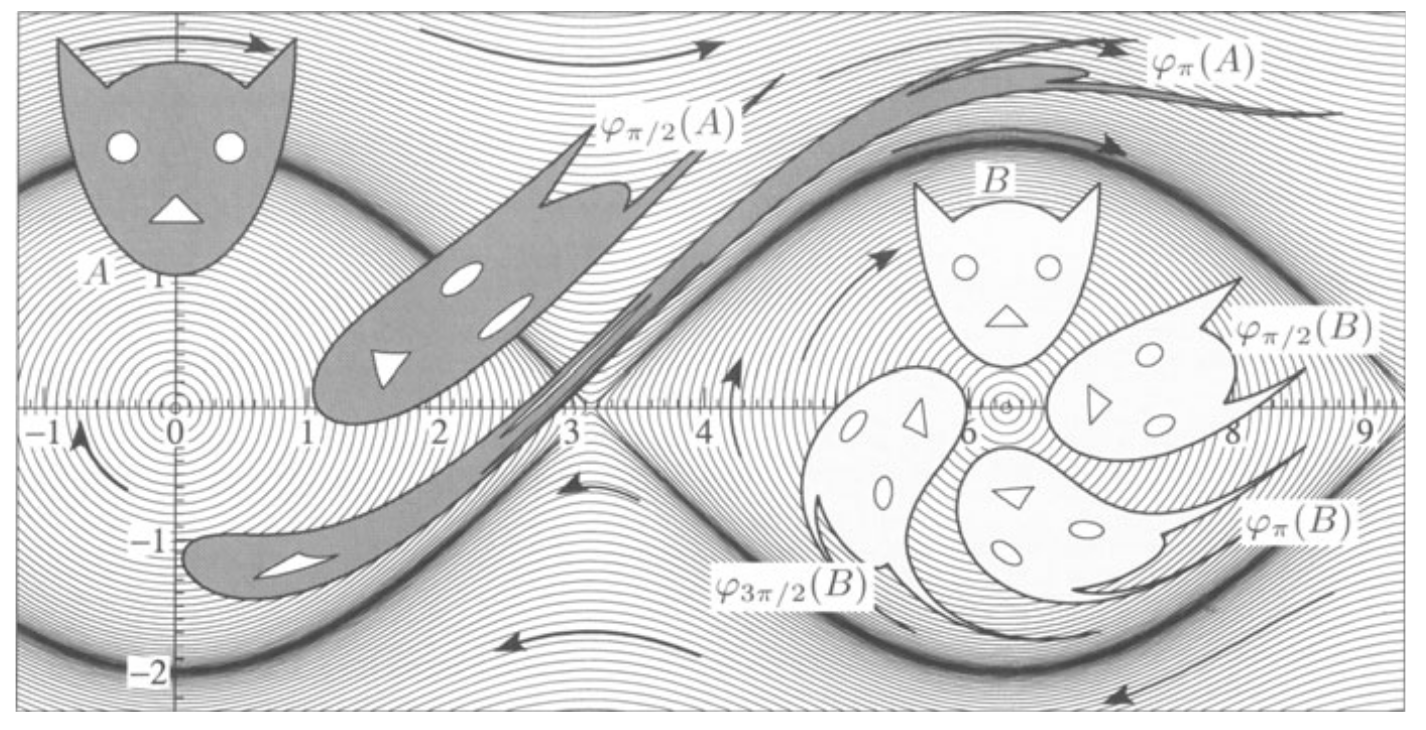
\includegraphics[width=0.8\textwidth]{pendulum-symplecticity-cats}
	\end{center}
\end{bsp}



Betrachte die Hamiltonschen Gleichungen
\begin{equation*}
	\dot p = - \frac{\partial H}{\partial q}(p, q),
	\quad
	\dot q = \frac{\partial H}{\partial p}(p, q)
\end{equation*}

Umschreiben:
\begin{equation*}
	\begin{pmatrix} \dot p \\ \dot q \end{pmatrix}
	=
	\begin{pmatrix} 0 & I \\ -I & 0 \end{pmatrix}^{-1}
	\begin{pmatrix} \frac{\partial H}{\partial p} \\ \frac{\partial H}{\partial q} \end{pmatrix}
\end{equation*}

Diese Beziehung wollen wir jetzt abstrakter betrachten.

\begin{bem}
	Die harmlos aussehende Matrix $\left(\begin{smallmatrix} 0 & I \\ -I & 0 \end{smallmatrix}\right)$ hat eine besondere Eigenschaft.
	Es gilt nämlich
	\begin{equation*}
		\begin{pmatrix} 0 & I \\ -I & 0 \end{pmatrix}^2
		= - \begin{pmatrix} I & 0 \\ 0 & I \end{pmatrix}.
	\end{equation*}
	Sie verhält sich also wie die imaginäre Einheit $i$ und erzeugt damit eine komplexe Struktur auf $\R^{2d}$.
\end{bem}

Wir betrachten $2$-dimensionale Parallelogramme in $\R^{2d}$ aufgespannt durch Vektoren
\begin{equation*}
	\xi = \begin{pmatrix} \xi^p \\ \xi^q \end{pmatrix},
	\quad
	\eta = \begin{pmatrix} \eta^p \\ \eta^q \end{pmatrix}.
\end{equation*}
Hier und im Folgenden bezeichnen $\xi^p \in \R^d$ und $\xi^q \in \R^d$ die Impuls- bzw.\ Ortskomponenten
von $\xi$.

Falls $d = 1$, so ist die orientierte Fläche des Parallelogramms gerade
\begin{equation*}
	\det\begin{pmatrix} \xi^p & \eta^p \\ \xi^q & \eta^q \end{pmatrix}
	= \xi^p \eta^q - \xi^q \eta^p
	= (\xi^p \quad \xi^q)
	\begin{pmatrix} 0 & 1 \\ -1 & 0 \end{pmatrix}
	\begin{pmatrix} \eta^p \\ \eta^q \end{pmatrix}.
\end{equation*}

Das verallgemeinern wir jetzt für höhere Dimensionen.

\begin{definition}[Symplektische Form]
	Die symplektische Form $\omega: \R^{2d} \times \R^{2d} \to \R$ ist
	\begin{equation*}
		\omega(\xi, \eta)
		\colonequals \sum_{i=1}^d \det\begin{pmatrix} \xi_i^p & \eta_i^p \\ \xi_i^q & \eta_i^q \end{pmatrix}
		= \sum_{i=1}^d \left( \xi_i^p \eta_i^q - \xi_i^q \eta_i^p \right).
	\end{equation*}
\end{definition}

\begin{itemize}
	\item Bilineare Form
	\item Interpretation: Summe der orientierten Flächen der Projektionen auf die Koordinatenebenen $(p_i, q_i)$.
	\item Matrixdarstellung
	\begin{equation*}
		\omega(\xi, \eta) =
		\begin{pmatrix} {\xi^p}^T & {\xi^q}^T \end{pmatrix}
		\begin{pmatrix} 0 & I \\ -I & 0 \end{pmatrix}
		\begin{pmatrix} \eta^p \\ \eta^q \end{pmatrix}.
	\end{equation*}
\end{itemize}

Da die Matrix $\begin{pmatrix} 0 & I \\ -I & 0 \end{pmatrix}$ wichtig zu sein scheint geben wir ihr den Namen $J$.

Eine wichtige Eigenschaft von Hamiltonschen Systemen ist nun, dass ihre Flüsse $\Phi^t \colon \R^{2d} \to \R^{2d}$ die symplektische Form erhalten. Das muss man natürlich erklären.

\begin{definition}[Lineare symplektische Abbildung]
	Eine lineare Abbildung $A: \R^{2d} \to \R^{2d}$ heißt \emph{symplektisch}, wenn
	\begin{equation*}
		\omega(A\xi, A\eta) = \omega(\xi, \eta) \qquad \forall \xi, \eta \in \R^{2d}.
	\end{equation*}
	Alternativ: wenn $A^T J A = J$.
\end{definition}

\begin{bem}
	Für $d=1$ bedeutet das gerade, dass $A$ flächenerhaltend ist.
\end{bem}

\begin{definition}[Differenzierbare symplektische Abbildung]
	Sei $U$ eine offene Teilmenge von $\R^{2d}$.
	Eine differenzierbare Abbildung $g: U \to \R^{2d}$ heißt \begriff{symplektisch}, falls die Jacobi-Matrix $\nabla g(p,q)$ für alle $(p, q) \in U$ symplektisch ist.
\end{definition}

Jetzt kommt der zentrale Satz: die Flüsse $\Phi^t$ von Hamiltonschen Systemen erhalten die symplektische Form:

\begin{satz}[Poincaré, 1899]
	Sei $H(p, q)$ zweimal stetig differenzierbar auf $U \subset \R^{2d}$.
	Sei $\Phi^t$ der Phasenfluss der Differentialgleichung
	\begin{equation*}
		\dot y = J^{-1} \nabla H(y)
	\end{equation*}
	mit $y = (p, q)$.

	Für jedes feste $t$ ist $\Phi^t$ eine symplektische Abbildung.
\end{satz}

\begin{proof}
	Der Beweis erfolgt in zwei Schritten:
	\begin{enumerate}
		\item $\Phi^0$ ist symplektisch.
		\item Die \enquote{Abweichung von der Symplektizität} hängt nicht von $t$ ab.
	\end{enumerate}
	
	\begin{enumerate}[label=(zu \arabic*), leftmargin=*]
		\item $\Phi^0$ ist symplektisch, wenn seine erste Ableitung an jedem Punkt $y_0 = (p_0, q_0)$ symplektisch ist. Da $\Phi^0 y_0 = y_0$ gilt
		\begin{equation*}
			\left( \frac{\partial \Phi^0 y_0}{\partial y_0} \right)^T J \left( \frac{\partial \Phi^0 y_0}{\partial y_0} \right)
			= I^T J I
			= J
		\end{equation*}
		Also ist $\Phi^0$ symplektisch.
		
		\item Wir müssen die Ableitung $\frac{\partial \Phi^t y_0}{\partial y_0}$ untersuchen, d.h. die linearisierte Störung der Lösung bei einer Störung des Startwerts -- also gerade die Wronski-Matrix $\Xi$. Diese löst die Gleichung
		\begin{equation*}
			\dot \Xi = J^{-1} \underbrace{\nabla^2 H( \Phi^t(y_0) )}_{\text{Hesse-Matrix von $H$}} \Xi
		\end{equation*}
		Konkret heißt das hier
		\begin{equation}
			\label{eq:wronski_symplectic_form}
			\frac{d}{dt} \frac{\partial \Phi^t}{\partial y_0}
			= J^{-1} \nabla^2 H(\Phi^t y_0) \frac{\partial \Phi^t}{\partial y_0}
		\end{equation}
		Die Produktregel liefert uns
		\begin{equation*}
			\frac{d}{dt}\bigg[ \bigg(\frac{\partial \Phi^t}{\partial y_0}\bigg)^T J \bigg(\frac{\partial \Phi^t}{\partial y_0}\bigg) \bigg]
			= \bigg( \frac{d}{dt} \frac{\partial \Phi^t}{\partial y_0} \bigg)^T J \bigg( \frac{\partial \Phi^t}{\partial y_0} \bigg)
			+ \bigg( \frac{\partial \Phi^t}{\partial y_0} \bigg)^T J \bigg( \frac{d}{dt} \frac{\partial \Phi^t}{\partial y_0} \bigg)
		\end{equation*}
		Dort wird jetzt \eqref{eq:wronski_symplectic_form} eingesetzt:
		\begin{equation*}
			\frac{d}{dt}\bigg[ \bigg(\frac{\partial \Phi^t}{\partial y_0}\bigg)^T J \bigg(\frac{\partial \Phi^t}{\partial y_0}\bigg) \bigg]
			=
			\bigg(\frac{\partial \Phi^t}{\partial y_0}\bigg)^T \nabla^2 H(\Phi^t y_0)^T J^{-T} J \bigg(\frac{\partial \Phi^t}{\partial y_0}\bigg)
			+ \bigg(\frac{\partial \Phi^t}{\partial y_0}\bigg)^T J J^{-1} \nabla^2 H(\Phi^t y_0) \bigg(\frac{\partial \Phi^t}{\partial y_0}\bigg)
		\end{equation*}
		Aber $J^T = -J$, also $J^{-T} J = -I$, und $\nabla^2 H$ ist symmetrisch. Deshalb ist
		\begin{equation*}
			\frac{d}{dt}\bigg[ \bigg(\frac{\partial \Phi^t}{\partial y_0}\bigg)^T
			J
			\bigg(\frac{\partial \Phi^t}{\partial y_0}\bigg) \bigg]
			= 0
		\end{equation*}
	\end{enumerate}
\end{proof}

Es gilt sogar die Umkehrung des Satzes:
\textit{nur} Hamiltonsche Systeme haben symplektische Flüsse!

\begin{definition}[lokal Hamiltonsch]
	Eine Differentialgleichung $x' = f(x)$ heißt \begriff{lokal Hamiltonsch}, wenn für jedes $x_0 \in U$ eine Umgebung existiert, in der
	\begin{equation*}
		f(x) = J^{-1} \nabla H(x)
	\end{equation*}
	für eine Funktion $H$.
\end{definition}

\begin{satz}[{{{\cite[Satz~VI.2.6]{hairer_lubich_wanner:2006}}}}]
	Sei $f \colon U \to \R^{2d}$ stetig differenzierbar.
	Dann ist $x' = f(x)$ genau dann lokal Hamiltonsch, wenn der Fluss $\Phi^t x$ für alle $x \in U$ und alle $t$ hinreichend klein symplektisch ist.
\end{satz}




\section{Symplektische Verfahren}

Wir wollen Verfahren entwickeln, die die Symplektizität von Hamiltonschen Flüssen erben.

\begin{definition}
	Ein Einschrittverfahren heißt symplektisch, falls der diskrete Fluss
	\begin{equation*}
		\Psi^t \colon \R^{2d}\to\R^{2d}
	\end{equation*}
	symplektisch ist, wenn das Verfahren auf ein Hamiltonsches System angewendet wird.
\end{definition}

Die einfachsten symplektischen Verfahren sind die symplektischen Euler-Verfahren
\begin{align*}
	p_{k+1} &= p_k - \tau H_q(p_{k+1},q_k) \\
	q_{k+1} &= q_k + \tau H_p(p_{k+1},q_k)
\end{align*}
und
\begin{align*}
	p_{k+1} &= p_k - \tau H_q(p_k,q_{k+1}) \\
	q_{k+1} &= q_k + \tau H_p(p_k,q_{k+1}).
\end{align*}

\begin{satz}[{{\cite[Satz~VI.3.3]{hairer_lubich_wanner:2006}}}]
	Die symplektischen Euler-Verfahren sind symplektisch.
\end{satz}
\begin{proof}
	Beweis für die erste Methode:
	\begin{itemize}
		\item Methode ist symplektisch, wenn
		\begin{equation*}
		\frac{\partial\Psi^\tau y}{\partial y}\in \R^{2d\times 2d}
		\end{equation*}
		für alle $y=(p,q)$ die symplektisch Form erhält, wenn also
		\begin{equation}\label{eq:symplektische_form}
		\Big(\frac{\partial\Psi^\tau y}{\partial y}\Big)^TJ\Big(\frac{\partial\Psi^\tau y}{\partial y}\Big) = J.
		\end{equation}
		\item Wir bestimmen die vier Komponenten von $\frac{\partial\Psi^\tau y}{\partial y}$:
		\item [1)] Erste Gleichung des Verfahrens:
		\begin{equation*}
		p_{k+1} = p_k - \tau H_q(p_{k+1},q_k)
		\end{equation*}
		Ableiten nach $p_k$:
		\begin{equation*}
		\frac{\partial p_{k+1}}{\partial p_k} = I - \tau H_{qp}(p_{k+1},q_k)\cdot \frac{\partial p_{k+1}}{\partial p_k}
		\end{equation*}
		$\Leftrightarrow$
		\begin{equation*}
		\frac{\partial p_{k+1}}{\partial p_k}\Big(I + \tau H_{qp}\Big) = I
		\end{equation*}
		Ebenso z.B.
		\begin{equation*}
		\frac{\partial p_{k+1}}{\partial q_k}\Big(I + \tau H_{qp}\Big) = -\tau H_{qq}
		\end{equation*}
		etc.
	\end{itemize}
	Zusammen erhält man
	\begin{equation*}
	\begin{pmatrix}
	I + \tau H_{qp}^T & 0 \\ -\tau H_{pp} & I
	\end{pmatrix}
	\begin{pmatrix}
	\frac{\partial p_{k+1}}{\partial p_k} & 	\frac{\partial p_{k+1}}{\partial q_k} \\
	\frac{\partial q_{k+1}}{\partial p_k}  & 	\frac{\partial q_{k+1}}{\partial q_k}
	\end{pmatrix}
	=
	\begin{pmatrix}
	I & -\tau H_{qq} \\ 0 & I+\tau H_{qp}
	\end{pmatrix},
	\end{equation*}
	also
	\begin{equation*}
	\frac{\partial \Psi^\tau y}{\partial y} = \begin{pmatrix}
	I + \tau H_{qp}^T & 0 \\ -\tau H_{pp} & I
	\end{pmatrix}^{-1} \begin{pmatrix}
	I & -\tau H_{qq} \\ 0 & I+\tau H_{qp}
	\end{pmatrix}.
	\end{equation*}
	Damit kann man die Erhaltungseigenschaft \eqref{eq:symplektische_form} direkt nachrechnen.
\end{proof}

Die symplektischen Euler-Verfahren sind \emph{keine} RK-Verfahren. 
Stattdessen gehören sie zu den sog.\ \emph{partitionierten} RK-Verfahren.
Betrachte Differentialgleichungen der Form
\begin{equation*}
	y'=f(y,z),\qquad z'=g(y,z),
\end{equation*}
wobei $y\in\R^{n_1}$ und $z\in\R^{n_2}$. 

\textbf{Idee:} Nimm für $y$ und $z$ zwei verschiedene RK-Verfahren.
Details bei \cite[Kapitel II.2]{hairer_lubich_wanner:2006}

Es gibt auch ein \enquote{einfaches} Verfahren zweiter Ordnung, das symplektisch ist.
\begin{satz}[{{\cite[Satz~VI.3.5]{hairer_lubich_wanner:2006}}}]
	Die implizite Mittelpunktsregel
	\begin{equation*}
		y_{k+1} = y_k + \tau J^{-1}\nabla H\Big( \frac{y_{k+1}+y_k}{2}\Big)
	\end{equation*}
	ist symplektisch.
\end{satz}
\begin{proof}
	Wir leiten wieder ab
	\begin{align*}
		\frac{\partial \Psi^\tau y_k}{\partial y_k} &= \frac{\partial y_{k+1}}{\partial y_k} \\
		&= I + \tau J^{-1} \nabla^2 H\Big( \frac{y_{k+1} + y_k}{2} \Big) \cdot \Big( \frac{1}{2} \frac{\partial y_{k+1}}{y_k} + \frac{1}{2}\Big).
	\end{align*}
	Umformen ergibt
	\begin{align*}
		\frac{\partial y_{k+1}}{\partial y_k}
		&= \Big( I - \frac{\tau}{2} J^{-1}\nabla^2H\Big)^{-1}\Big(I+\frac{\tau}{2}J^{-1}\nabla^2 H\Big).
	\end{align*}
	Dann kann man direkt nachrechnen dass
	$\Big(\frac{\partial y_{k+1}}{\partial y_k}\Big)^T J \frac{\partial y_{k+1}}{\partial y_k} = J$.

	\todoannot{1.5\baselineskip}{Ein paar Details zu dieser Rechnung einfügen!}
\end{proof}


\subsection{Symplektische RK-Verfahren}

Dabei handelt es sich um relativ neue Verfahren, die erst Ende der 1980er Jahre systematisch untersucht wurden.

Wir interessieren uns wieder für die Ableitung
\begin{equation*}
	\Xi(t) = \frac{\partial \Phi^t y_0}{\partial y_0}.
\end{equation*}
Diese löst bekanntlich eine lineare Differentialgleichung.

\begin{lemma}[{{\cite[Lemma VI.4.1]{hairer_lubich_wanner:2006}}}]
	Das folgende Diagramm kommutiert für alle Runge-Kutta-Verfahren und alle partitionierten Runge-Kutta-Verfahren:\\
	\begin{center}
		\begin{tikzpicture}
		\draw (0,0)  node{$\{y_k\}$};
		\draw[->] (1,0) -- node[above]{$\frac{\partial}{\partial y_0}$} (3,0); 
		\draw (5,0) node{$\{y_k,\Xi_k\}$};
		\draw[->] (0,2)-- node[left]{RK-Verfahren}(0,1);
		\draw[->] (5,2)-- node[right]{RK-Verfahren}(5,1);
		\draw[->] (1,3)-- node[above]{$\frac{\partial}{\partial y_0}$}(3,3);
		\draw (-1,3)  node{$\dot y = f(y),\ y(0)=y_0$};
		\draw (5.5,3.2)  node{$\dot y = f(y),\quad y(0)=y_0$};
		\draw (5.5,2.7)  node{$\dot\Xi = f'(y)\Xi,\quad \Xi(0)=I$};
		\end{tikzpicture}
	\end{center}
\end{lemma}
\begin{proof}[Beweisidee:] Betrachte exemplarisch das explizite Euler-Verfahren
	\begin{equation*}
		y_{k+1} = y_k +\tau f(y_k).
	\end{equation*}
	Ableiten nach $y_0$ ergibt
	\begin{equation*}
		\Xi_{k+1} = \Xi_k + \tau f'(y_k)\Xi_k.
	\end{equation*}
	Das ist gerade das explizite Euler-Verfahren für die Gleichung
	\begin{equation*}
		\dot \Xi = f'(y)\Xi.
	\end{equation*}
	Startwert passt auch, denn $I=\frac{\partial y_0}{\partial y_0} = \Xi_0$.
\end{proof}


\begin{idea}
	Die Symplektizitätsbedingung ist eine quadratische Invariante des
	erweiterten Systems für die Variablen $y$ und $\Xi$.
\end{idea}

\begin{satz}
	Alle Verfahren die quadratische Invarianten erhalten sind symplektisch.
\end{satz}
\begin{proof}
	Der quadratische Ausdruck $\Xi^T J\Xi$ is Invariante der Gleichung
	\begin{equation*}
		\dot \Xi = J^{-1}\nabla^2 H(y)\Xi,
	\end{equation*}
	denn
	\begin{align*}
		\frac{d}{dt}\Big(\Xi^T J\Xi\Big) & = \dot \Xi^T J\Xi + \Xi^T J\dot\Xi \\
		& = (J^{-1}\nabla^2 H\Xi)^T J\Xi + \Xi^T JJ^{-1}\nabla^2 H \Xi \\
		& = \Xi^T \nabla^2 H \underbrace{J^{-T}J}_{=-I} + \Xi^T\underbrace{ JJ^{-1}}_{=I} \nabla^2 H \Xi \\
		& = 0
	\end{align*}
\end{proof}

\begin{kor}
	Gauß-Verfahren sind symplektisch.
\end{kor}

\subsection{Reversibilität vs.\ Symplektizität}

Es gibt reversible Verfahren, die nicht symplektisch sind.
Es gibt symplektische Verfahren, die nicht reversibel sind.

Für quadratische Hamilton-Funktionen ist das aber anders.

\begin{satz}[{{{\cite[Satz VI.4.9.]{hairer_lubich_wanner:2006}}}}]
	Für RK-Verfahren sind die folgenden Aussagen äquivalent:
	\begin{enumerate}[label=(\roman*)]
		\item Die Methode ist reversibel für lineare Probleme
		\begin{equation*}
			\dot y = Ly
		\end{equation*}
		\item Die Methode ist symplektisch für Hamilton-Gleichungen mit quadratischer Hamilton-Funktion
		\begin{equation*}
			H(y) = \frac{1}{2} y^TCy.\qquad C\ s.p.d.
		\end{equation*}
	\end{enumerate}
\end{satz}
\begin{proof}
	$ii) \to i)$\\
	\begin{itemize}
		\item Die Hamilton-Gleichungen haben die Form
		\begin{equation*}
		\dot y = J^{-1} \nabla H(y) = J^{-1}Cy,
		\end{equation*}
		sind also linear.
		\item Das Runge-Kutta-Verfahren dafür hat also die Form
		\begin{equation*}
		\Psi^\tau y = R(\tau J^{-1} C) y
		\end{equation*}
		wobei $R$ die Stabilitätsfunktion ist.
		\item Da das Verfahren symplektisch ist, gilt
		\begin{equation*}
		R(\tau J^{-1} C)^T J R(\tau J^{-1} C) = J.
		\end{equation*}
		
		\item Da $R= PQ^{-1}$ für Polynome $P,Q$ erhält man
		\begin{equation}\label{eq:beweis_symplektisch_symmetrisch}
		P(\tau J^{-1} C)^T JP(\tau J^{-1} C) = Q(\tau J^{-1} C)^T J Q(\tau J^{-1} C).
		\end{equation}
		
		\item Betrachte das Produkt \glqq Polynom in $J^{-1} C$\grqq\ mit $J$.
		
		\item Für jedes Monom $(J^{-1} C)^k$, $k \in \N$ gilt
		($C$ ist symmetrisch, und $J^T = -J$)
		\begin{align*}
		((J^{-1} C)^k)^T J
		& =
		(C^T J^{-T})^k J \\
		& =
		\underbrace{C^TJ^{-T} \dots C^TJ^{-T}}_{\text{$k$ mal}} J \\
		& =
		-C^T\underbrace{J^{-T}C^T \dots J^{-T}C^T}_{\text{$k-1$ mal}} \\
		& =
		-C\underbrace{J^{-T}C \dots J^{-T}C}_{\text{$k-1$ mal}} \\
		& =
		-J^T J^{-T} C\underbrace{J^{-T}C \dots J^{-T}C}_{\text{$k-1$ mal}} \\
		& =
		-J^T (J^{-T}C)^k \\
		& =
		J(-J^{-1} C)^k.
		\end{align*}
		\item Also folgt aus \eqref{eq:beweis_symplektisch_symmetrisch}
		\begin{equation*}
		P(-\tau J^{-1} C)\cdot P(\tau J^{-1} C) =  Q(-\tau J^{-1} C)\cdot Q(\tau J^{-1} C)
		\end{equation*}
		bzw.
		\begin{equation*}
		R(-\tau J^{-1} C)\cdot R(\tau J^{-1} C) = I.
		\end{equation*}
		\item  Das ist gerade die Reversibilität des Verfahrens.
	\end{itemize}
\end{proof}

\section{Energieerhaltung}

Wir haben einige Mühe in Verständnis und Erhaltung der Symplektizität gesteckt.
Aber Symplektizität ist eine sehr abstrakte Eigenschaft. Wozu soll die gut sein? Hier komme eine etwas konkretere Rechtfertigung.

Betrachte das mathematische Pendel.
\begin{itemize}
	\item Kinetische Energie:
	\begin{equation*}
		T(q, \dot q) = \frac{m l^2}{2} \dot q
	\end{equation*}
	($q$ ist der Winkel)
	\item Potentielle Energie:
	\begin{equation*}
		U(q) = -mgl \cos q
	\end{equation*}
	\item Bewegungsgleichungen:
	\begin{equation*}
		\ddot q + \frac gl \sin q = 0
	\end{equation*}
	\item Gesamtenergie:
	\begin{equation*}
		E = \frac{m l^2}2 \dot q^2 - mgl \cos q
	\end{equation*}
	Dies entspricht der Hamilton-Funktion
	\begin{equation*}
		H(p, q) = \frac{1}{2ml^2} p^2 - mgl \cos q
	\end{equation*}
	Damit ist die Gesamtenergie eine Erhaltungsgröße!
	\item Aber: weder linear noch quadratisch.
	Wird daher nicht automatisch von z.B. Gauß-Verfahren erhalten.
\end{itemize}

Wird die Energie von symplektischen Verfahren erhalten?

Nein! Aber fast...

\begin{satz}[{{{\cite{benettin_giorgilli:1994}; \cite[Thm.\,IX.8.1]{hairer_lubich_wanner:2006}}}}]
	Betrachte ein Hamilton-System mit analytischer Hamilton-Funktion $H: D \to R$ ($D \subset \R^{2d}$) und wende ein symplektisches Verfahren $\Psi^\tau$ mit Schrittweite $\tau$ an. Wenn die numerische Lösung in einer kompakten Menge $K\subset D$ bleibt, dann existiert ein $\tau_0$, so dass
	\begin{equation*}
		H(y_n) = H(y_0) + O(\tau^p) %\vadjust{\todo{$H$ ist nicht ganz konstant, aber die Abweichung ist seeeehr klein - nämlich in $\mathcal{O}(\tau^p)$}}
	\end{equation*}
	für exponentiell lange Zeitintervalle $n\tau \le e^{\frac{\tau_0}{2 \tau}}$.
\end{satz}

Symplektische Verfahren erhalten also \emph{nicht} die Hamilton-Funktion bzw.\ die Gesamtenergie. Aber die numerische Energie bleibt \enquote{in der Nähe} der exakten Energie!


\section{Variationelle Integratoren}

Mit dem jetzt Gelernten können wir Zeitschrittverfahren auf eine ganz neue Art konstruieren.
Siehe dazu \cite{marsden_west:2001} für eine detailliertere Übersicht.

Wir erinnern an das Prinzip der stationären Wirkung (auch Hamiltonsches Prinzip genannt): 
Lagrange-Funktion
\begin{equation*}
	L(q,\dot q) = T(q,\dot q) - U(q)
\end{equation*}

\begin{definition}
	Die \begriff{Wirkung} eine Trajektorie $q\colon t\mapsto (q(t),\dot q(t))$ ist
	\begin{equation*}
		S(q)\coloneqq \int_{t_0}^{t_1} L(q(t),\dot q(t))\,dt.
	\end{equation*}
\end{definition}

Wir betrachten nur Trajektorien mit gegebenem festen Start- und Endpunkt
\begin{equation*}
	q(t_0) = q_0,\qquad q(t_1) = q_1.
\end{equation*}

\begin{definition}[Hamiltonsches Prinzip]
	Die tatsächlich vorkommenden Trajektorien sind die, die die Wirkung stationär machen.
\end{definition}

Sei $q$ eine Trajektorie, und $\delta q$ eine Variation davon, die die Endpunkte fest lässt, also $\delta q(t_0)=\delta(t_1) = 0$.
Stationarität von $q$ heißt dann, dass für alle solche $\delta q$
\begin{equation*}
	\frac{d}{d\epsilon} S(q+\epsilon\delta q)\big\vert_{\epsilon=0} = 0.
\end{equation*}
Wie schon in Kapitel~\ref{sec:lagrange_gleichung} gezeigt ist dies äquivalent zur Euler--Lagrange-Gleichung
\begin{equation*}
	\frac{d}{dt}\frac{\partial L}{\partial \dot q} = \frac{\partial L}{\partial q}.
\end{equation*}

Wir betrachten jetzt das Wirkungsintegral $S$ als Funktion der Start- und Endposition
\begin{equation*}
	S(q_0,q_1) = \int_{t_0}^{t_1} L(q(t),\dot q(t))\,dt.
\end{equation*}
Dabei ist $q$ die zu $q_0,q_1$ gehörige Lösung der Lagrange-Gleichung.

\subsubsection*{Exkurs Anfang: Erzeugendenfunktionen}

Wir brauchen ein weiteres Kriterium für Symplektizität:
\begin{itemize}
	\item Betrachte ein gegebenes Hamiltonsches System $H$ auf einem festen Zeitintervall $[t_0,t_1]$
	\item Seien $p_0 \in \R^d$ und $q_0 \in \R^d$ die Startwerte zur Zeit $t_0$
	\item Bezeichne die Werte zur Zeit $t_1$ mit  $p_1 \in \R^d$ und $q_1 \in \R^d$
	\item Es gibt eine Abbildung $\Phi^{t_0,t_1}(p_0,q_0) = (p_1,q_1)$.
\end{itemize}

Wie wir wissen, ist diese symplektisch.
{[Achtung: der folgende Satz enthält überdurchschnittlich viel didaktische Reduktion]}

\begin{satz}[{{\cite[Satz VI.5.1]{hairer_lubich_wanner:2006}}}]
	\label{thm:erzeugendenfunktion}
	Eine Abbildung $\varphi\colon (p_0,q_0) \mapsto (p_1,q_1)$ ist genau dann symplektisch, wenn lokal eine Funktion
	\begin{equation*}
		S\colon (q_0,q_1)\mapsto S(q_0,q_1)\in\R
	\end{equation*}
	existiert, so dass
	\begin{equation}\label{eq:abbildung_symplektisch}
		\nabla S 0
		\begin{pmatrix}
		\frac{\partial S}{\partial q_0}  \\
		\frac{\partial S}{\partial q_1}
		\end{pmatrix} = \begin{pmatrix}
		-p_0 \\ p_1
		\end{pmatrix}
	\end{equation}
\end{satz}

Wenn man eine symplektische Abbildung $(p_0,q_0)\mapsto(p_1,q_1)$ hat, dann kann sie durch \eqref{eq:abbildung_symplektisch} aus der Funktion $S$ rekonstruiert werden.

Aber der obige Satz ist vom Typ \enquote{Äquivalenz}. Es gilt also auch die Umkehrung: Jede hinreichen glatte (und in einem gewissen Sinne nicht degenerierte) Funktion $S$ \emph{erzeugt} via \eqref{eq:abbildung_symplektisch} eine symplektische Abbildung $(p_0,q_0)\mapsto (p_1,q_1)$.\note{Hier muss noch was hin.}

Man kann also auf systematische Art symplektische Abbildungen erzeugen. Die Funktion $S$ heißt deshalb Erzeugendenfunktion.

\subsubsection*{Exkurs Ende}

Große Überraschung: Diese Funktion $S$ ist gerade die Erzeugendenfunktion einer symplektischen Abbildung!

Berechne die partielle Ableitung:
\begin{align*}
	\frac{\partial S}{\partial q_0}
	& =
	\int_{t_0}^{t_1} \bigg( \frac{\partial L}{\partial q} \frac{\partial q}{\partial q_0} + \frac{\partial L}{\partial \dot q}\frac{\partial\dot q}{\partial q_0}\bigg)\,dt \\
	%
	\intertext{Partielle Integration des zweiten Terms in der Klammer liefert}
	&=
	\frac{\partial L}{\partial \dot q}\frac{\partial q}{\partial q_0}\Bigg\vert_{t_0}^{t_1} + \int_{t_0}^{t_1} \underbrace{\bigg( \frac{\partial L}{\partial q}  - \frac{d}{dt} \frac{\partial L}{\partial \dot q}\bigg)}_{=0} \frac{\partial q}{\partial q_0}\,dt \\
	&= \frac{\partial L(q_1,\dot q_1)}{\partial \dot q} \cdot \underbrace{\frac{\partial q_1}{\partial q_0}}_{=0}  - \frac{\partial L(q_0,\dot q_0)}{\partial \dot q} \cdot \underbrace{\frac{\partial q_0}{\partial q_0}}_{=1}  \\
	&= - \frac{\partial L(q_0,\dot q_0)}{\partial \dot q} \\
	&= -p_0 \tag{Def. des Impulses}
\end{align*}
Ebenso berechnet man
\begin{equation*}
	\frac{\partial S}{\partial q_1} = p_1.
\end{equation*}
Wir erhalten also
\begin{equation}
	\nabla S =
	\begin{pmatrix}
	\frac{\partial S}{\partial q_0}  \\
	\frac{\partial S}{\partial q_1}
	\end{pmatrix}
	=
	\begin{pmatrix}
	-p_0 \\ p_1
	\end{pmatrix}
\end{equation}
Dies ist gerade die Formel \eqref{eq:abbildung_symplektisch} für Erzeugendenfunktionen von symplektischen Abbildungen.

Daraus folgt dass die entsprechende Abbildung $(p_0,q_0) \mapsto (p_1,q_1)$ symplektisch ist.

\subsection{Idee der variationellen Integratoren}

Wir ersetzen das Integral im Hamiltonschen Prinzip durch eine diskrete Approximation:

Wir führen ein Zeitgitter $t_0<t_1<\hdots < t_N = T$ und die approximative Wirkung
\begin{equation*}
	L_h(q_k,q_{k+1})\approx \int_{t_k}^{t_{k+1}} L(q(t),\dot q(t))\,dt
\end{equation*}
ein (z.B.\ durch eine Quadraturformel).

Hier könnte man denken dass $L_h$ ein schlechtes Symbol ist, weil es sich ja schließlich um eine Wirkung handelt. Andererseits fungiert $L_h$ später bei der Definition der diskreten Impulse wie eine Lagrange-Funktion (siehe~\eqref{eq:diskrete_lagrange_transformation}).

$q$ ist hier die Lösung der Lagrange-Gleichung auf $[t_k,t_{k+1}]$ mit gegebenen Start- und Endwerten $q_k,q_{k+1}$.
	
Definiere das diskrete Wirkungsfunktional
\begin{equation*}
	S_h\Big(\big\{q_k\big\}_{k=0}^N\Big) \colonequals \sum_{k=0}^{N-1} L_h(q_k,q_{k+1})
\end{equation*}

\begin{definition}[Diskretes Hamilton-Prinzip]
	Finde $\{q_k\}^N_{k=0}$  mit gegebenen $q_0, q_N$, so dass $S_h$ stationär wird.
\end{definition}

Wie kann man $L_h$ wählen?

\begin{bsp}[{{\cite[1992]{mackay:1992}}}]
	Approximiere $q$ auf $[t_k, t_{k+1}]$ als linear Interpolierende von $q_k$ und $q_{k+1}$.
	
	Approximiere das Integral durch die Trapezregel
	\begin{equation*}
		L_h(q_k, q_{k+1}) =
		\tau \cdot \frac{1}{2} \Big[L\Big(q_k, \frac{q_{k+1} - q_k}{\tau}\Big) +  L\Big(q_{k+1}, \frac{q_{k+1} - q_k}{\tau}\Big)\Big].
	\end{equation*}
\end{bsp}

\begin{bsp}[{{\cite[1997]{wendlandt_marsden:1997}}}]
	Nimm statt der Trapezregel die Mittelpunktsregel
	\begin{equation*}
		L_h(q_k, q_{k+1}) = \tau \Big[L\Big(\frac{q_{k+1} + q_k}{2}, \frac{q_{k+1} - q_k}{\tau}\Big)\Big].
	\end{equation*}
\end{bsp}


Wie kommen wir an stationäre Punkte von $S_h$?

Wir können die Ableitung ausrechnen und gleich Null setzen --- partielle Ableitung für $k=1, \dots, N-1$:
\begin{equation*}
	\frac{\partial S_h}{\partial q_k}
	=
	\frac{\partial}{\partial q_k} \sum_{i=0}^{N-1} L_h (q_i, q_{i+1})
	=
	\frac{\partial}{\partial q_k} L_h(q_{k-1}, q_k) +  \frac{\partial}{\partial q_k} L_h(q_k, q_{k+1})
\end{equation*}
Dieser Ausdruck $=0$ sind die \emph{diskreten Euler--Lagrange-Gleichungen} -- ein System von algebraischen Gleichungen (mit Bandstruktur).

\textbf{Fragen:}
\begin{itemize}
	\item Wann kriege ich mit diesem Ansatz symplektische Integratoren?
	\item Kann ich das Verfahren so umschreiben dass ich wieder einen Zeitschritt nach dem anderen berechnen kann?
\end{itemize}




%%%%%%%%%%%%%%%%%%%%%%%%%%%%%%%%%%%%%%%%%%%%%%%%%%%%%%%%%%%%%%%%%%%%%%%%%%%%%%%%%%%%%%%%%%%%%%%%%%%%%%%%%%%%%%%%%%%%%%%%%%%%%%%%%%%%%%%%%%%%%%%%%%%%


%\section{Symplektizität}
%
%Flüsse von Hamiltonschen Systemen haben eine weitere wichtige Erhaltungseigenschaft,
%\begin{itemize}
%\item die sog. Symplektizität
%\item ähnlich wie Volumenerhaltung im Phasenraum
%\end{itemize}
%
%\emph{Beispiel}: Volumenerhaltung beim mathematischen Pendel
%
%  \bigskip
%  \todoannot{1.5\baselineskip}{Bild}
%
%Betrachte die Hamiltonschen Gleichungen
%\begin{equation*}
%  \dot p = - \frac{\partial H}{\partial q}(p, q),
%  \quad
%  \dot q = \frac{\partial H}{\partial p}(p, q)
%\end{equation*}
%
%Umschreiben:
%\begin{equation*}
%  \begin{pmatrix} \dot p \\ \dot q \end{pmatrix}
%  =
%  \begin{pmatrix} 0 & I \\ -I & 0 \end{pmatrix}^{-1}
%  \begin{pmatrix} \frac{\partial H}{\partial p} \\ \frac{\partial H}{\partial q} \end{pmatrix}
%\end{equation*}
%
%Diese Beziehung wollen wir jetzt abstrakter betrachten.
%
%Bemerke: die harmlos aussehende Matrix $\begin{pmatrix} 0 & I \\ -I & 0 \end{pmatrix}$ hat eine besondere Eigenschaft.
%Es gilt nämlich
%\begin{equation*}
%  \begin{pmatrix} 0 & I \\ -I & 0 \end{pmatrix}^2
%  = - \begin{pmatrix} I & 0 \\ 0 & I \end{pmatrix}.
%\end{equation*}
%\begin{itemize}
%\item Verhält sich also wie die imaginäre Einheit $i$.
%\item Erzeugt eine komplexe Struktur auf $\R^{2d}$.
%\end{itemize}
%
%Wir betrachten 2-dimensionale Parallelogramme in $\R^{2d}$.
%\begin{itemize}
%\item Aufgespannt durch Vektoren
%  \begin{equation*}
%    \xi = \begin{pmatrix} \xi^p \\ \xi^q \end{pmatrix},
%    \quad
%    \eta = \begin{pmatrix} \eta^p \\ \eta^q \end{pmatrix}.
%  \end{equation*}
%\end{itemize}
%
%Falls $d = 1$, so ist die orientierte Fläche des Parallelogramms gerade
%\begin{equation*}
%  \det\begin{pmatrix} \xi^p & \eta^p \\ \xi^q & \eta^q \end{pmatrix}
%  =
%  \xi^p \eta^q - \xi^q \eta^p
%  =
%  (\xi^p \quad \xi^q)
%  \begin{pmatrix} 0 & 1 \\ -1 & 0 \end{pmatrix}
%  \begin{pmatrix} \eta^p \\ \eta^q \end{pmatrix}.
%\end{equation*}
%Das verallgemeinern wir jetzt für höhere Dimensionen.
%
%\begin{definition}[Symplektische Form]
%  Die symplektische Form $\omega: \R^{2d} \times \R^{2d} \to \R$ ist
%  \begin{equation*}
%    \omega(\xi, \eta)
%    \colonequals \sum_{i=1}^d \det\begin{pmatrix} \xi_i^p & \eta_i^p \\ \xi_i^q & \eta_i^q \end{pmatrix}
%    = \sum_{i=1}^d \left( \xi_i^p \eta_i^q - \xi_i^q \eta_i^p \right).
%  \end{equation*}
%\end{definition}
%
%\begin{itemize}
%\item Bilineare Form
%\item Interpretation: Summe der orientierten Flächen der Projektionen auf die Koordinatenebenen $(p_i, q_i)$.
%\item Matrixdarstellung
%  \begin{equation*}
%    \omega(\xi, \eta)
%    =
%    \begin{pmatrix} {\xi^p}^T & {\xi^q}^T \end{pmatrix}
%    \begin{pmatrix} 0 & I \\ -I & 0 \end{pmatrix}
%    \begin{pmatrix} \eta^p \\ \eta^q \end{pmatrix}.
%  \end{equation*}
%\end{itemize}
%
%Da die Matrix $\begin{pmatrix} 0 & I \\ -I & 0 \end{pmatrix}$ wichtig zu sein scheint geben wir ihr den Namen $J$.
%
%Eine wichtige Eigenschaft von Hamiltonschen Systemen ist nun, dass ihre Flüsse
%\begin{equation*}
%  \Phi^t: \R^{2d} \to \R^{2d}
%\end{equation*}
%die symplektische Form erhalten.
%
%Das muss man natürlich erklären.
%
%\begin{definition}[Lineare symplektische Abbildung]
%  Eine lineare Abbildung $A: \R^{2d} \to \R^{2d}$ heißt \emph{symplektisch}, wenn
%  \begin{equation*}
%    \omega(A\xi, A\eta) = \omega(\xi, \eta) \qquad \forall \xi, \eta \in \R^{2d}.
%  \end{equation*}
%  Alternativ: Wenn
%  \begin{equation*}
%    A^T J A = J.
%  \end{equation*}
%\end{definition}
%
%\begin{itemize}
%\item Für $d=1$ bedeutet das gerade, dass $A$ flächenerhaltend ist.
%\end{itemize}
%
%\begin{definition}[Differenzierbare symplektische Abbildung]
%  Sei $U$ eine offene Teilmenge von $\R^{2d}$.
%  Eine differenzierbare Abbildung $g: U \to \R^{2d}$ heißt \emph{symplektisch}, falls die Jacobi-Matrix $\nabla g(p,q)$ für alle $(p, q) \in U$ symplektisch ist.
%\end{definition}
%
%Jetzt der zentrale Satz:
%die Flüsse $\Phi^t$ von Hamiltonschen Systemen erhalten die symplektische Form:
%
%\begin{satz}[Poincaré, 1899]
%  Sei $H(p, q)$ zweimal stetig differenzierbar auf $U \subset \R^{2d}$.
%  Sei $\Phi^t$ der Phasenfluss der Differentialgleichung
%  \begin{equation*}
%    \dot y = J^{-1} \nabla H(y)
%  \end{equation*}
%  mit $y = (p, q)$.
%
%  Für jedes feste $t$ ist $\Phi^t$ eine symplektische Abbildung.
%\end{satz}
%
%\begin{proof}
% Der Beweis erfolgt in zwei Schritten:
%  \begin{enumerate}
%  \item $\Phi^0$ ist symplektisch.
%  \item Die \glqq Abweichung von der Symplektizität\grqq{} hängt nicht von $t$ ab.
%  \end{enumerate}
%
%  Zu 1):
%  \begin{itemize}
%  \item $\Phi^0$ ist symplektisch, wenn seine erste Ableitung an jedem Punkt $y_0 = (p_0, q_0)$ symplektisch ist.
%  \item Da $\Phi^0 y_0 = y_0$ gilt
%    \begin{equation*}
%      \left( \frac{\partial \Phi^0 y_0}{\partial y_0} \right)^T J \left( \frac{\partial \Phi^0 y_0}{\partial y_0} \right)
%      = I^T J I
%      = J.
%    \end{equation*}
%  \item Also ist $\Phi^0$ symplektisch.
%  \end{itemize}
%
%  Zu 2):
%  \begin{itemize}
%  \item Wir müssen die Ableitung $\frac{\partial \Phi^t y_0}{\partial y_0}$ untersuchen.
%  \item Linearisierte Störung der Lösung bei einer Störung des Startwerts.
%  \item Also gerade die Wronski-Matrix $\Xi$
%  \item Löst die Gleichung
%    \begin{equation*}
%      \dot \Xi = J^{-1} \underbrace{\nabla^2 H( \Phi^t(y_0) )}_{\text{Hesse-Matrix von $H$}} \Xi
%    \end{equation*}
%
%  \item Konkret heißt das hier
%    \begin{equation}
%     \label{eq:wronski_symplectic_form}
%      \frac{d}{dt} \frac{\partial \Phi^t}{\partial y_0}
%      = J^{-1} \nabla^2 H(\Phi^t y_0) \frac{\partial \Phi^t}{\partial y_0}
%    \end{equation}
%
%
%  \item Produktregel:
%   \begin{equation*}
%    \frac{d}{dt}\bigg[ \bigg(\frac{\partial \Phi^t}{\partial y_0}\bigg)^T J \bigg(\frac{\partial \Phi^t}{\partial y_0}\bigg) \bigg]
%    = \bigg( \frac{d}{dt} \frac{\partial \Phi^t}{\partial y_0} \bigg)^T J \bigg( \frac{\partial \Phi^t}{\partial y_0} \bigg)
%    + \bigg( \frac{\partial \Phi^t}{\partial y_0} \bigg)^T J \bigg( \frac{d}{dt} \frac{\partial \Phi^t}{\partial y_0} \bigg)
%    \end{equation*}
%
%   \item Dort wird jetzt \eqref{eq:wronski_symplectic_form} eingesetzt:
%    \begin{equation*}
%      \frac{d}{dt}\bigg[ \bigg(\frac{\partial \Phi^t}{\partial y_0}\bigg)^T J \bigg(\frac{\partial \Phi^t}{\partial y_0}\bigg) \bigg]
%      =
%      \bigg(\frac{\partial \Phi^t}{\partial y_0}\bigg)^T \nabla^2 H(\Phi^t y_0)^T J^{-T} J \bigg(\frac{\partial \Phi^t}{\partial y_0}\bigg)
%      + \bigg(\frac{\partial \Phi^t}{\partial y_0}\bigg)^T J J^{-1} \nabla^2 H(\Phi^t y_0) \bigg(\frac{\partial \Phi^t}{\partial y_0}\bigg)
%    \end{equation*}
%  \item Aber $J^T = -J$, also $J^{-T} J = -I$, und $\nabla^ H$ ist symmetrisch.
%  \item Deshalb ist
%    \begin{equation*}
%      \frac{d}{dt}\bigg[ \bigg(\frac{\partial \Phi^t}{\partial y_0}\bigg)^T
%        J
%        \bigg(\frac{\partial \Phi^t}{\partial y_0}\bigg) \bigg]
%      = 0.
%      \qedhere
%    \end{equation*}
%  \end{itemize}
%\end{proof}
%
%Es gilt sogar die Umkehrung des Satzes:
%\emph{nur} Hamiltonsche Systeme haben symplektische Flüsse!
%
%\begin{definition}[lokal Hamiltonsch]
%  Eine Differentialgleichung $x' = f(x)$ heißt \emph{lokal Hamiltonsch}, wenn für jedes $x_0 \in U$ eine Nachbarschaft existiert, in der
%  \begin{equation*}
%    f(x) = J^{-1} \nabla H(x)
%  \end{equation*}
%  für eine Funktion $H$.
%\end{definition}
%
%\begin{satz}[{\citet[Satz~VI.2.6]{hairer_lubich_wanner:2006}}]
%  Sei $f: U \to \R^{2d}$ stetig differenzierbar.
%  Dann ist $x' = f(x)$ genau dann lokal Hamiltonsch, wenn der Fluss $\Phi^t x$ für alle $x \in U$ und alle $t$ hinreichend klein symplektisch ist.
%\end{satz}
%
%\section{Symplektische Verfahren}
%
%Wir wollen Verfahren entwickeln, die die Symplektizität von Hamiltonschen Flüssen erben.
%
%\begin{definition}
%	Ein Einschrittverfahren heißt symplektisch, falls der diskrete Fluss
%	\begin{equation*}
%		\Psi^t\colon \R^{2d}\to\R^{2d}
%	\end{equation*}
%	symplektisch ist, wenn das Verfahren auf ein Hamiltonsches System angewendet wird.
%\end{definition}
%
%Die einfachsten symplektischen Verfahren sind die symplektischen Euler-Verfahren
%\begin{align*}
%	p_{k+1} &= p_k - \tau H_q(p_{k+1},q_k) \\
%	q_{k+1} &= q_k + \tau H_p(p_{k+1},q_k)
%\end{align*}
%und
%\begin{align*}
%	p_{k+1} &= p_k - \tau H_q(p_k,q_{k+1}) \\
%	q_{k+1} &= q_k + \tau H_p(p_k,q_{k+1}).
%\end{align*}
%
%\begin{satz}[{\citet[Satz~VI.3.3]{hairer_lubich_wanner:2006}}]
%	Die symplektischen Euler-Verfahren sind symplektisch.
%\end{satz}
%\begin{proof}
%	Beweis für die erste Methode:
%	\begin{itemize}
%		\item Methode ist symplektisch, wenn
%		\begin{equation*}
%			\frac{\partial\Psi^\tau y}{\partial y}\in \R^{2d\times 2d}
%		\end{equation*}
%		für alle $y=(p,q)$ die symplektisch Form erhält, wenn also
%		\begin{equation}\label{eq:symplektische_form}
%			\Big(\frac{\partial\Psi^\tau y}{\partial y}\Big)^TJ\Big(\frac{\partial\Psi^\tau y}{\partial y}\Big) = J.
%		\end{equation}
%		\item Wir bestimmen die vier Komponenten von $\frac{\partial\Psi^\tau y}{\partial y}$:
%		\item [1)] Erste Gleichung des Verfahrens:
%			\begin{equation*}
%				p_{k+1} = p_k - \tau H_q(p_{k+1},q_k)
%			\end{equation*}
%			Ableiten nach $p_k$:
%			\begin{equation*}
%				\frac{\partial p_{k+1}}{\partial p_k} = I - \tau H_{qp}(p_{k+1},q_k)\cdot \frac{\partial p_{k+1}}{\partial p_k}
%			\end{equation*}
%			$\Leftrightarrow$
%			\begin{equation*}
%				\frac{\partial p_{k+1}}{\partial p_k}\Big(I + \tau H_{qp}\Big) = I
%			\end{equation*}
%			Ebenso z.B.
%			\begin{equation*}
%				\frac{\partial p_{k+1}}{\partial q_k}\Big(I + \tau H_{qp}\Big) = -\tau H_{qq}
%			\end{equation*}
%			etc.
%	\end{itemize}
%Zusammen erhält man
%\begin{equation*}
%	\begin{pmatrix}
%		I + \tau H_{qp}^T & 0 \\ -\tau H_{pp} & I
%	\end{pmatrix}
%	\begin{pmatrix}
%		\frac{\partial p_{k+1}}{\partial p_k} & 	\frac{\partial p_{k+1}}{\partial q_k} \\
%			\frac{\partial q_{k+1}}{\partial p_k}  & 	\frac{\partial q_{k+1}}{\partial q_k}
%	\end{pmatrix}
%	=
%	\begin{pmatrix}
%		I & -\tau H_{qq} \\ 0 & I+\tau H_{qp}
%	\end{pmatrix},
%\end{equation*}
%also
%\begin{equation*}
%	\frac{\partial \Psi^\tau y}{\partial y} = \begin{pmatrix}
%	I + \tau H_{qp}^T & 0 \\ -\tau H_{pp} & I
%	\end{pmatrix}^{-1} \begin{pmatrix}
%	I & -\tau H_{qq} \\ 0 & I+\tau H_{qp}
%	\end{pmatrix}.
%\end{equation*}
%Damit kann man die Erhaltungseigenschaft \eqref{eq:symplektische_form} direkt nachrechnen.
%\end{proof}
%
%\medskip
%
%Die symplektischen Euler-Verfahren sind \emph{keine} RK-Verfahren.\\
%Stattdessen gehören sie zu den sog.\ \emph{partitionierten} RK-Verfahren.\\
%Betrachte Differentialgleichungen der Form
%\begin{equation*}
%	y'=f(y,z),\qquad z'=g(y,z),
%\end{equation*}
%wobei $y\in\R^{n_1}$ und $z\in\R^{n_2}$\\
%\emph{Idee:} Nimm für $y$ und $z$ zwei verschiedene RK-Verfahren.\\
%Details bei \citet[Kapitel II.2]{hairer_lubich_wanner:2006}
%
%\medskip
%
%Es gibt auch ein \glqq einfaches\grqq\ Verfahren zweiter Ordnung, das symplektisch ist.
%\begin{satz}[{\citet[Satz~VI.3.5]{hairer_lubich_wanner:2006}}]
%	Die implizite Mittelpunktsregel
%	\begin{equation*}
%		y_{k+1} = y_k + \tau J^{-1}\nabla H\Big( \frac{y_{k+1}+y_k}{2}\Big)
%	\end{equation*}
%	ist symplektisch.
%\end{satz}
%\begin{proof}
%	Wir leiten wieder ab
%	\begin{align*}
%		\frac{\partial \Psi^\tau y_k}{\partial y_k} &= \frac{\partial y_{k+1}}{\partial y_k} \\
%		&= I + \tau J^{-1} \nabla^2 H\Big( \frac{y_{k+1} + y_k}{2} \Big) \cdot \Big( \frac{1}{2} \frac{\partial y_{k+1}}{y_k} + \frac{1}{2}\Big).
%	\end{align*}
%Umformen ergibt
%\begin{align*}
% \frac{\partial y_{k+1}}{\partial y_k}
% &=
% \Big( I - \frac{\tau}{2} J^{-1}\nabla^2H\Big)^{-1}\Big(I+\frac{\tau}{2}J^{-1}\nabla^2 H\Big).
%\end{align*}
%
%	Dann kann man direkt nachrechnen dass
%	$\Big(\frac{\partial y_{k+1}}{\partial y_k}\Big)^T J \frac{\partial y_{k+1}}{\partial y_k} = J$.
%
% \bigskip
%\todoannot{1.5\baselineskip}{Ein paar Details zu dieser Rechnung einfügen!}
%\end{proof}
%
%
%\subsection{Symplektische RK-Verfahren}
%
%\begin{itemize}
%	\item Relativ neue Verfahren, wurden erst Ende der 1980er Jahre systematisch untersucht.
%\end{itemize}
%
%Wir interessieren uns wieder für die Ableitung
%\begin{equation*}
%\Xi(t) = \frac{\partial \Phi^t y_0}{\partial y_0}.
%\end{equation*}
%Diese löst bekanntlich eine lineare Differentialgleichung.
%
%\begin{lemma}[{\citet[Lemma VI.4.1]{hairer_lubich_wanner:2006}}]
%	
%	Das folgende Diagramm kommutiert für alle Runge-Kutta-Verfahren und alle partitionierten Runge-Kutta-Verfahren:\\
%	\begin{center}
%	    \begin{tikzpicture}
%	    	\draw (0,0)  node{$\{y_k\}$};
%	    	\draw[->] (1,0) -- node[above]{$\frac{\partial}{\partial y_0}$} (3,0); 
%	    	\draw (5,0) node{$\{y_k,\Xi_k\}$};
%	    	\draw[->] (0,2)-- node[left]{RK-Verfahren}(0,1);
%	    	\draw[->] (5,2)-- node[right]{RK-Verfahren}(5,1);
%	    	\draw[->] (1,3)-- node[above]{$\frac{\partial}{\partial y_0}$}(3,3);
%	    	\draw (-1,3)  node{$\dot y = f(y),\ y(0)=y_0$};
%	    	\draw (5.5,3.2)  node{$\dot y = f(y),\quad y(0)=y_0$};
%	    	\draw (5.5,2.7)  node{$\dot\Xi = f'(y)\Xi,\quad \Xi(0)=I$};
%	    \end{tikzpicture}
%	\end{center}
%\end{lemma}
%\begin{proof}[Beweisidee:] Betrachte exemplarisch das explizite Euler-Verfahren
%\begin{equation*}
%	y_{k+1} = y_k +\tau f(y_k).
%\end{equation*}
%Ableiten nach $y_0$ ergibt
%\begin{equation*}
%	\Xi_{k+1} = \Xi_k + \tau f'(y_k)\Xi_k.
%\end{equation*}
%Das ist gerade das explizite Euler-Verfahren für die Gleichung
%\begin{equation*}
%	\dot \Xi = f'(y)\Xi.
%\end{equation*}
%Startwert passt auch, denn $I=\frac{\partial y_0}{\partial y_0} = \Xi_0$.
%\end{proof}
%
%\bigskip
%
%\emph{Idee:} Die Symplektizitätsbedingung ist eine quadratische invariante des
%erweiterten Systems für die Variablen $y$, $\Xi$.
%
%
%\begin{satz}
%	Alle Verfahren die quadratische Invarianten erhalten sind symplektisch.
%\end{satz}
%\begin{proof}
%	Der quadratische Ausdruck $\Xi^T J\Xi$ is Invariante der Gleichung
%	\begin{equation*}
%		\dot \Xi = J^{-1}\nabla^2 H(y)\Xi,
%	\end{equation*}
%	denn
%	\begin{align*}
%		\frac{d}{dt}\Big(\Xi^T J\Xi\Big) & = \dot \Xi^T J\Xi + \Xi^T J\dot\Xi \\
%		                                 & = (J^{-1}\nabla^2 H\Xi)^T J\Xi + \Xi^T JJ^{-1}\nabla^2 H \Xi \\
%		                                 & = \Xi^T \nabla^2 H \underbrace{J^{-T}J}_{=-I} + \Xi^T\underbrace{ JJ^{-1}}_{=I} \nabla^2 H \Xi \\
%		                                 & = 0.  \qedhere
%	\end{align*}
%\end{proof}
%
%\begin{kor}
%	Gauß-Verfahren sind symplektisch.
%\end{kor}
%
%\subsection{Reversibilität vs.\ Symplektizität}
%
%Es gibt reversible Verfahren, die nicht symplektisch sind.
%
%\medskip
%
%Es gibt symplektische Verfahren, die nicht reversibel sind.
%
%\medskip
%
%Für quadratische Hamilton-Funktionen ist das anders.
%
%\begin{satz}[{\citet[Satz VI.4.9.]{hairer_lubich_wanner:2006}}]
%	Für RK-Verfahren sind die folgenden Aussagen äquivalent:
%	\begin{itemize}
%		\item [i)] Die Methode ist reversibel für lineare Probleme
%		\begin{equation*}
%			\dot y = Ly
%		\end{equation*}
%		\item [ii)] Die Methode ist symplektisch für Hamilton-Gleichungen mit quadratischer Hamilton-Funktion
%		\begin{equation*}
%			H(y) = \frac{1}{2} y^TCy.\qquad C\ s.p.d.
%		\end{equation*}
%	\end{itemize}
%\end{satz}
%\begin{proof}
%	$ii) \to i)$\\
%	\begin{itemize}
%		\item Die Hamilton-Gleichungen haben die Form
%		\begin{equation*}
%			\dot y = J^{-1} \nabla H(y) = J^{-1}Cy,
%		\end{equation*}
%		sind also linear.
%
%		\item Das Runge-Kutta-Verfahren dafür hat also die Form
%		\begin{equation*}
%			\Psi^\tau y = R(\tau J^{-1} C) y
%		\end{equation*}
%		wobei $R$ die Stabilitätsfunktion ist.
%		\item Da das Verfahren symplektisch ist, gilt
%		\begin{equation*}
%			R(\tau J^{-1} C)^T J R(\tau J^{-1} C) = J.
%		\end{equation*}
%
%		\item Da $R= PQ^{-1}$ für Polynome $P,Q$ erhält man
%		\begin{equation}\label{eq:beweis_symplektisch_symmetrisch}
%			P(\tau J^{-1} C)^T JP(\tau J^{-1} C) = Q(\tau J^{-1} C)^T J Q(\tau J^{-1} C).
%		\end{equation}
%
%\todoannot{1.5\baselineskip}{Die folgende Rechnung muss nochmal im Detail überprüft werden!}
%
%		\item Betrachte das Produkt \glqq Polynom in $J^{-1} C$\grqq\ mit $J$.
%
%		\item Für jedes Monom $(J^{-1} C)^k$ gilt ($C$ ist symmetrisch)
%		\begin{equation*}
%			((J^{-1} C)^k)^T J
%			=
%			(C^T J^{-T})^k J
%			=
%			J(-(J^{-1} C)^k)\quad \forall k=0,1,2,\hdots
%		\end{equation*}
%		\item Also folgt aus \eqref{eq:beweis_symplektisch_symmetrisch}
%		\begin{equation*}
%			P(-\tau J^{-1} C)\cdot P(\tau J^{-1} C) =  Q(-\tau J^{-1} C)\cdot Q(\tau J^{-1} C)
%		\end{equation*}
%		bzw.
%		\begin{equation*}
%			R(-\tau J^{-1} C)\cdot R(\tau J^{-1} C) = I.
%		\end{equation*}
%		\item  Das ist gerade die Symmetrie des Verfahrens.
%		\qedhere
%	\end{itemize}
%\end{proof}
%
%\section{Energieerhaltung}
%
%\begin{itemize}
%\item Wir haben einige Mühe in Verständnis und Erhaltung der Symplektizität gesteckt.
%\item Aber Symplektizität ist eine sehr abstrakte Eigenschaft.
%  Wozu soll die gut sein?
%\item Hier komme eine etwas konkretere Rechtfertigung.
%\end{itemize}
%
%Betrachte das mathematische Pendel.
%\begin{itemize}
%\item Kinetische Energie:
%  \begin{equation*}
%    T(q, \dot q) = \frac{m l^2}{2} \dot q
%  \end{equation*}
%  ($q$ ist der Winkel)
%\item Potentielle Energie:
%  \begin{equation*}
%    U(q) = -mgl \cos q
%  \end{equation*}
%\item Bewegungsgleichungen:
%  \begin{equation*}
%    \ddot q + \frac gl \sin q = 0
%  \end{equation*}
%\item Gesamtenergie:
%  \begin{equation*}
%    E = \frac{m l^2}2 \dot q^2 - mgl \cos q
%  \end{equation*}
%  Dies entspricht der Hamilton-Funktion
%  \begin{equation*}
%    H(p, q) = \frac{1}{2ml^2} p^2 - mgl \cos q
%  \end{equation*}
%  Damit ist die Gesamtenergie eine Erhaltungsgröße!
%\item Aber: weder linear noch quadratisch.
%  Wird daher nicht automatisch von z.B. Gauß-Verfahren erhalten.
%\end{itemize}
%
%Wird die Energie von symplektischen Verfahren erhalten?
%
%Nein! Aber fast...
%
%\begin{satz}[{\citet{benettin_giorgilli:1994}; \citet[Thm.\,IX.8.1]{hairer_lubich_wanner:2006}}]
%  Betrachte ein Hamilton-System mit analytischer Hamilton-Funktion $H: D \to R$, ($D \subset \R^{2d}$),
%  und wende ein symplektisches Verfahren $\Psi^\tau$ mit Schrittweite $\tau$ an.
%  Wenn die numerische Lösung in einer kompakten Menge $K\subset D$ bleibt, dann existiert ein $\tau_0$, so dass
%  \begin{equation*}
%    H(y_n) = H(y_0) + O(\tau^p)
%  \end{equation*}
%  für exponentiell lange Zeitintervalle $n\tau \le e^{\frac{\tau_0}{2 \tau}}$.
%\end{satz}
%
%Symplektische Verfahren erhalten also \emph{nicht} die Hamilton-Funktion bzw.\ die Gesamtenergie.
%Aber die numerische Energie bleibt \glqq in der Nähe\grqq{} der exakten Energie!
%
%
%
%\section{Variationelle Integratoren}
%
%Mit dem jetzt Gelernten können wir Zeitschrittverfahren auf eine ganz neue Art konstruieren.\\
%Siehe \citet{marsden_west:2001} für eine detailliertere Übersicht.\\
%
%Wir erinnern an das Prinzip der stationären Wirkung (auch Hamiltonsches Prinzip genannt)
%\begin{itemize}
%	\item Lagrange-Funktion
%	\begin{equation*}
%		L(q,\dot q) = T(q,\dot q) - U(q)
%	\end{equation*}
%\end{itemize}
%
%\begin{definition}
% Die \emph{Wirkung} eine Trajektorie $q\colon t\mapsto (q(t),\dot q(t))$ ist
%	\begin{equation*}
%		S(q)\coloneqq \int_{t_0}^{t_1} L(q(t),\dot q(t))\,dt.
%	\end{equation*}
%\end{definition}
%
%\medskip
%
% Wir betrachten nur Trajektorien mit gegebenem festen Start- und Endpunkt
%	\begin{equation*}
%		q(t_0) = q_0,\qquad q(t_1) = q_1.
%	\end{equation*}
%
%\begin{definition}[Hamiltonsches Prinzip]
%Die tatsächlich vorkommenden Trajektorien sind die, die die Wirkung stationär machen.
%\end{definition}
%
%Sei $q$ eine Trajektorie, und $\delta q$ eine Variation davon, die die Endpunkte fest lässt, also $\delta q(t_0)=\delta(t_1) = 0$.
%\begin{itemize}
%	\item Stationarität von $q$ heißt dann, dass für alle solche $\delta q$
%	\begin{equation*}
%		\frac{d}{d\epsilon} S(q+\epsilon\delta q)\Big\vert_{\epsilon=0} = 0.
%	\end{equation*}
%\end{itemize}
%Wie schon in Kapitel~\ref{sec:lagrange_gleichung} gezeigt ist dies äquivalent zur Euler--Lagrange-Gleichung
%\begin{equation*}
%	\frac{d}{dt}\frac{\partial L}{\partial \dot q} = \frac{\partial L}{\partial q}.
%\end{equation*}
%
%\bigskip
%
%Wir betrachten jetzt das Wirkungsintegral $S$ als Funktion der Start- und Endposition
%\begin{equation*}
%	S(q_0,q_1) = \int_{t_0}^{t_1} L(q(t),\dot q(t))\,dt.
%\end{equation*}
%Dabei ist $q$ die zu $q_0,q_1$ gehörige Lösung der Lagrange-Gleichung.\\
%
%\subsubsection*{Exkurs Anfang: Erzeugendenfunktionen}
%
%Wir brauchen ein weiteres Kriterium für Symplektizität:
%\begin{itemize}
%	\item Betrachte ein gegebenes Hamiltonsches System $H$ auf einem festen Zeitintervall $[t_0,t_1]$
%	\item Seien $p_0 \in \R^d$ und $q_0 \in \R^d$ die Startwerte zur Zeit $t_0$
%	\item Bezeichne die Werte zur Zeit $t_1$ mit  $p_1 \in \R^d$ und $q_1 \in \R^d$
%	\item Es gibt eine Abbildung $\Phi^{t_0,t_1}(p_0,q_0) = (p_1,q_1)$.
%\end{itemize}
%
%Wie wir wissen, ist diese symplektisch.\\
%{[Achtung: der folgende Satz enthält überdurchschnittlich viel didaktische Reduktion]}
%
%\begin{satz}[{\citet[Satz VI.5.1]{hairer_lubich_wanner:2006}}]
%\label{thm:erzeugendenfunktion}
%	Eine Abbildung $\varphi\colon (p_0,q_0) \mapsto (p_1,q_1)$ ist genau dann symplektisch, wenn lokal eine Funktion
%	\begin{equation*}
%	S\colon (q_0,q_1)\mapsto S(q_0,q_1)\in\R
%	\end{equation*}
%	existiert, so dass
%	\begin{equation}\label{eq:abbildung_symplektisch}
%	\nabla S
%	=
%	\begin{pmatrix}
%		\frac{\partial S}{\partial q_0}  \\
%		\frac{\partial S}{\partial q_1}
%	\end{pmatrix} = \begin{pmatrix}
%		-p_0 \\ p_1
%	\end{pmatrix}.
%	\end{equation}
%\end{satz}
%
%\begin{itemize}
%	\item Wenn man eine symplektische Abbildung $(p_0,q_0)\mapsto(p_1,q_1)$ hat, dann sie durch \eqref{eq:abbildung_symplektisch} aus der Funktion $S$ rekonstruiert werden.
%	\item Aber der obige Satz ist \glqq genau dann, wenn\grqq\ . Es gilt also auch die Umkehrung:
%	\begin{itemize}
%		\item Jede hinreichen glatte (und in einem gewissen Sinne nicht degenerierte)
%		 Funktion $S$ \emph{erzeugt} via \eqref{eq:abbildung_symplektisch} eine symplektische Abbildung $(p_0,q_0)\mapsto (p_1,q_1)$!
%	\end{itemize}
%	\item Man kann also auf systematische Art symplektische Abbildungen erzeugen. Die Funktion $S$ heißt deshalb Erzeugendenfunktion.
%\end{itemize}
%
%
%\subsubsection*{Exkurs Ende}
%
%Große Überraschung: Diese Funktion $S$ ist gerade die Erzeugendenfunktion einer symplektischen Abbildung!
%\begin{itemize}
% \item Berechne partielle Ableitung:
%  \begin{align*}
%   \frac{\partial S}{\partial q_0}
%   & =
%   \int_{t_0}^{t_1} \bigg( \frac{\partial L}{\partial q} \frac{\partial q}{\partial q_0} + \frac{\partial L}{\partial \dot q}\frac{\partial\dot q}{\partial q_0}\bigg)\,dt \\
%   %
%   \intertext{Partielle Integration des zweiten Terms in der Klammer liefert}
%   &=
%   \frac{\partial L}{\partial \dot q}\frac{\partial q}{\partial q_0}\Bigg\vert_{t_0}^{t_1} + \int_{t_0}^{t_1} \underbrace{\bigg( \frac{\partial L}{\partial q}  - \frac{d}{dt} \frac{\partial L}{\partial \dot q}\bigg)}_{=0} \frac{\partial q}{\partial q_0}\,dt \\
%		&= \frac{\partial L(q_1,\dot q_1)}{\partial \dot q} \cdot \underbrace{\frac{\partial q_1}{\partial q_0}}_{=0}  - \frac{\partial L(q_0,\dot q_0)}{\partial \dot q} \cdot \underbrace{\frac{\partial q_0}{\partial q_0}}_{=1}  \\
%		&= - \frac{\partial L(q_0,\dot q_0)}{\partial \dot q} \\
%		&= -p_0 \qquad\text{(Def. des Impulses)}.
%	\end{align*}
%\end{itemize}
%Ebenso berechnet man
%\begin{equation*}
%	\frac{\partial S}{\partial q_1} = p_1.
%\end{equation*}
%Wir erhalten also
%\begin{equation}
%\nabla S =
%\begin{pmatrix}
%\frac{\partial S}{\partial q_0}  \\
%\frac{\partial S}{\partial q_1}
%\end{pmatrix}
%=
%\begin{pmatrix}
%-p_0 \\ p_1
%\end{pmatrix}.
%\end{equation}
%Dies ist gerade die Formel \eqref{eq:abbildung_symplektisch} für Erzeugendenfunktionen von symplektischen Abbildungen.
%
%Daraus folgt dass die entsprechende Abbildung $(p_0,q_0) \mapsto (p_1,q_1)$ symplektisch ist.
%
%\subsection{Idee der variationellen Integratoren}
%
%Wir ersetzen das Integral im Hamiltonschen Prinzip durch eine diskrete Approximation:
%
%\medskip
%
%\begin{itemize}
%	\item Führe ein Zeitgitter ein
%	\begin{equation*}
%	t_0<t_1<\hdots < t_N = T.
%	\end{equation*}
%	\item  Führe die approximative Wirkung ein
%	\begin{equation*}
%		L_h(q_k,q_{k+1})\approx \int_{t_k}^{t_{k+1}} L(q(t),\dot q(t))\,dt
%	\end{equation*}
%	(z.B.\ durch eine Quadraturformel)\\
%
%	Hier könnte man denken dass $L_h$ ein schlechtes Symbol ist, weil es sich ja schließlich
%	um eine Wirkung handelt.  Andererseits fungiert $L_h$ später bei der Definition der
%	diskreten Impulse wie eine Lagrange-Funktion (siehe~\eqref{eq:diskrete_lagrange_transformation}).
%
%	$q$ ist hier die Lösung der Lagrange-Gleichung auf $[t_k,t_{k+1}]$ mit gegebenen Start- und Endwerten $q_k,q_{k+1}$.
%	\item Definiere das diskrete Wirkungsfunktional
%	\begin{equation*}
%		S_h\Big(\big\{q_k\big\}_{k=0}^N\Big) \colonequals \sum_{k=0}^{N-1} L_h(q_k,q_{k+1}).
%	\end{equation*}
%\end{itemize}
%
%\begin{definition}[Diskretes Hamilton-Prinzip]
%Finde $\{q_k\}^N_{k=0}$  mit gegebenen $q_0, q_N$, so dass $S_h$ stationär wird.
%\end{definition}
%
%\medskip
%
%Wie kann man $L_h$ wählen?
%
%\medskip
%
%\emph{Beispiel:} (\citet{mackay:1992}, 1992)
%\begin{itemize}
%\item Approximiere $q$ auf $[t_k, t_{k+1}]$ als linear Interpolierende von $q_k$ und $q_{k+1}$.
%\item Approximiere das Integral durch die Trapezregel
%\begin{equation*}
%L_h(q_k, q_{k+1})
%=
%\tau \cdot \frac{1}{2} \Big[L\Big(q_k, \frac{q_{k+1} - q_k}{\tau}\Big) +  L\Big(q_{k+1}, \frac{q_{k+1} - q_k}{\tau}\Big)\Big].
%\end{equation*}
%\end{itemize}
%
%Beispiel: (\citet{wendlandt_marsden:1997}, 1997)
%\begin{itemize}
%\item Nimm statt der Trapezregel die Mittelpunktsregel
%\begin{equation*}
%L_h(q_k, q_{k+1}) = \tau \Big[L\Big(\frac{q_{k+1} + q_k}{2}, \frac{q_{k+1} - q_k}{\tau}\Big)\Big].
%\end{equation*}
%\end{itemize}
%
%Wie kommen wir an stationäre Punkte von $S_h$?
%\begin{itemize}
%\item Ableitung ausrechnen und gleich Null setzen!
%\newline Partielle Ableitung für $k=1, \dots, N-1$:
%\begin{equation*}
%\frac{\partial S_h}{\partial q_k}
%=
%\frac{\partial}{\partial q_k} \sum_{i=0}^{N-1} L_h (q_i, q_{i+1})
%=
%\frac{\partial}{\partial q_k} L_h(q_{k-1}, q_k) +  \frac{\partial}{\partial q_k} L_h(q_k, q_{k+1}).
%\end{equation*}
%\item Dieser Ausdruck $=0$ sind die \emph{diskreten Euler--Lagrange-Gleichungen}.
%\item Ein System von algebraischen Gleichungen (mit Bandstruktur).
%\end{itemize}
%
%\medskip
%
%\textbf{Fragen:}
%\begin{itemize}
%\item Wann kriege ich mit diesem Ansatz symplektische Integratoren?
%\item Kann ich das Verfahren so umschreiben dass ich wieder einen Zeitschritt nach dem anderen berechnen kann?
%\end{itemize}
%
%\subsection{Variationelle Integratoren sind symplektisch}
%
%Wir schreiben die diskrete Wirkung jetzt wieder als Funktion von Anfangs- und Endzustand
%\begin{equation*}
%S_h(q_0, q_N) = \sum_{k=0}^{N-1} L_h (q_k, q_{k+1}).
%\end{equation*}
%Dabei ist $\{q_k\}$ die dazugehörige Lösung des variationellen Integrators.
%\begin{itemize}
%\item Wir rechnen wieder die partiellen Ableitungen aus. Es bezeichne $\frac{\partial L_h}{\partial x}$,
%   $\frac{\partial L_h}{\partial y}$ die partiellen Ableitungen von $L_h$ nach dem ersten bzw.\ zweiten Argument:
%\begin{align*}
%\frac{\partial S_h}{\partial q_0}
%& = \sum_{k=0}^{N-1} \Bigg[ \frac{\partial L_h}{\partial x} \cdot\frac{\partial q_k}{\partial q_0} +  \frac{\partial L_h}{\partial y} \cdot\frac{\partial q_{k+1}}{\partial q_0}\Bigg] \\
%%
%& = \frac{\partial L}{\partial x} (q_0,q_1)\cdot \underbrace{\frac{\partial q_0}{\partial q_0}}_{=1} \\
%& \qquad  + \sum_{k=1}^{N-1} \Bigg[ \underbrace{\frac{\partial L_h}{\partial y}(q_{k-1},q_k) \cdot\frac{\partial q_k}{\partial q_0} +  \frac{\partial L_h}{\partial x} (q_k,q_{k+1})\cdot\frac{\partial q_k}{\partial q_0}}_{\text{$=0$, wg.\ diskreter Lagrange-Gleichung}}\Bigg] \\
%& \qquad \qquad  + \frac{\partial L_h}{\partial y} (q_{N-1},q_N)\cdot \underbrace{\frac{\partial q_N}{\partial q_0}}_{=0} \\
%%
%& =
%\frac{\partial L}{\partial x} (q_0, q_1).
%\end{align*}
%\item Ebenso 
%\begin{equation*}
%\frac{\partial S_h}{\partial q_N}  = \frac{\partial L_h}{\partial y} (q_{N-1}, q_N).
%\end{equation*}
%\end{itemize}
%Jetzt führen wir die \emph{diskreten Impulse} durch eine \emph{diskrete Legendre-Transformation} ein:
%\begin{equation}
%\label{eq:diskrete_lagrange_transformation}
% p_k
% \colonequals
% - \frac{\partial L_h}{\partial x} (q_k, q_{k+1})
% =
% \frac{\partial L_h}{\partial y} (q_{k-1}, q_k)
%\end{equation}
%Die Gleichheit ist gerade die diskrete Euler--Lagrange-Gleichung.
%
%[Vergleiche: $p = \frac{\partial L}{\partial \dot{q}}(q,\dot{q})$]
%
%\begin{itemize}
%\item Für $k=N$ erhalten wir
%\begin{equation*}
%p_N = \frac{\partial L_h}{\partial y} (q_{N-1}, q_N).
%\end{equation*}
%\end{itemize}
%
%\bigskip
%
%Zusammen also:
%\begin{equation*}
%\nabla S_h = \begin{pmatrix}
%\frac{\partial S_h}{\partial q_0} \\
%\frac{\partial S_h}{\partial q_N}
%\end{pmatrix} 
%=
%\begin{pmatrix}
%\frac{\partial L_h}{\partial x} (q_0, q_1) \\
%\frac{\partial L_h}{\partial y} (q_{N-1},q_N)
%\end{pmatrix}
%=
%\begin{pmatrix}
%- p_0 \\ p_N
%\end{pmatrix}
%\end{equation*}
%
%Nach Satz~\ref{thm:erzeugendenfunktion} ist $S_h$ also eine Erzeugendenfunktion für die symplektische Abbildung
%\begin{equation*}
%(p_0, q_0) \mapsto (p_N, q_N).
%\end{equation*} 
%
%\subsection{Variationelle Integratoren als klassische Einschrittverfahren}
%
%Jetzt bauen wir uns ein klassisches Zeitschrittverfahren:
%
%\medskip
%
%Angenommen die diskrete Legendre-Transformation \eqref{eq:diskrete_lagrange_transformation} sei eine Bijektion zwischen $p_k$ und $q_{k+1}$.
%
%Einschrittverfahren:
%\begin{center}
%    \begin{tikzpicture}
%      \draw (0,0)  node{$(p_k, q_k)$};
%      \draw[->] (0,-1) -- node[right]{inv. disk. Legendre-Transformation} (0,-2);
%      \draw (0,-3) node{$(q_k, q_{k+1})$};
%      \draw[->] (0,-4)-- node[right]{diskrete Euler--Lagrange-Gleichung}(0,-5);
%      \draw (0,-6) node{$(q_{k+1}, q_{k+2})$};
%      \draw[->] (0,-7)-- node[right]{diskrete Legendre-Transformation}(0,-8);
%      \draw (0,-9) node{$(p_{k+1}, q_{k+1})$};
%    \end{tikzpicture}
%\end{center}
%Schritt 2 und 3 schreibt man als
%\begin{equation*}
%p_{k+1} = \frac{\partial L_h}{\partial y} (q_k, q_{k+1}).
%\end{equation*}
%
%\begin{satz}
%Das diskrete Hamilton Prinzip erzeugt das Zeitschrittverfahren
%\begin{equation*}
%(p_k, q_k) \mapsto (p_{k+1}, q_{k+1}),
%\qquad
%p_k = - \frac{\partial L_h}{\partial x} (q_k, q_{k+1}),
%\qquad
%p_{k+1}  = \frac{\partial L_h}{\partial y} (q_k, q_{k+1}).
%\end{equation*}
%(Die erste Gleichung ist dabei als implizite Gleichung für $q_{k+1}$ zu verstehen.)
%\begin{itemize}
%\item[i)] Dieses Verfahren ist symplektisch.
%\item[ii)] Jedes symplektische Verfahren lässt sich auf diese Art darstellen.
%\end{itemize}
%\end{satz}
%\begin{proof}\mbox{} % Force line break
%\begin{itemize}
%  \item [i)] $L_h$ ist Erzeugendenfunktion für die symplektische Abbildung $(p_k, q_k) \mapsto (p_{k+1}, q_{k+1})$
%  \item [ii)] Jede symplektische Abbildung hat eine Erzeugendenfunktion. Wähle diese als diskrete Lagrange-Funktion.
%  \qedhere
%\end{itemize}
%\end{proof}
%
%\bigskip
%
%\emph{Beispiel:} Das Verfahren von \citet{mackay:1992}:
%\begin{equation*}
%L_h (q_k, q_{k+1}) = \frac{\tau}{2} L(q_k, v_{k + \frac{1}{2}}) + \frac{\tau}{2} L(q_{k+1}, v_{k + \frac{1}{2}})
%\end{equation*}
%mit $v_{k + \frac{1}{2}} \colonequals \frac{1}{\tau} (q_{k+1} - q_k)$.
%\newline
%\newline
%Man erhält das Verfahren:
%\begin{flalign*}
%p_k &= - \frac{\partial L_h}{\partial x} (q_k, q_{k+1}) \\
%&= - \frac{\tau}{2} \Big[ \frac{\partial L}{\partial q}(q_k, v_{k + \frac{1}{2}}) + \frac{\partial L}{\partial \dot{q}}(q_k, v_{k + \frac{1}{2}}) \cdot \Big(-\frac{1}{\tau}\Big) \\
%& \quad + \frac{\partial L}{\partial q}(q_{k+1}, v_{k + \frac{1}{2}}) \cdot \underbrace{\frac{\partial q_{k+1}}{\partial q_n}}_{=0} + \frac{\partial L}{\partial \dot{q}}(q_{k+1}, v_{k + \frac{1}{2}}) \cdot \Big(-\frac{1}{\tau}\Big) \Big] \\
%&= - \frac{\tau}{2}\frac{\partial L}{\partial q}(q_k, v_{k + \frac{1}{2}}) + \frac{1}{2} \frac{\partial L}{\partial \dot{q}}(q_k, v_{k + \frac{1}{2}}) +  \frac{1}{2}\frac{\partial L}{\partial \dot{q}}(q_{k+1}, v_{k + \frac{1}{2}}),
%\end{flalign*}
%sowie
%\begin{flalign*}
%p_{k+1}
%& =
%\frac{\partial L_h}{\partial y} (q_k, q_{k+1}) \\
%%
%&= \frac{\tau}{2}\frac{\partial L}{\partial q}(q_{k+1}, v_{k + \frac{1}{2}}) + \frac{1}{2} \frac{\partial L}{\partial \dot{q}}(q_k, v_{k + \frac{1}{2}}) +  \frac{1}{2}\frac{\partial L}{\partial \dot{q}}(q_{k+1}, v_{k + \frac{1}{2}}) .
%\end{flalign*}
%
%\medskip
%
%Wir betrachten das mechanische System
%\begin{equation*}
%L (q, \dot{q}) = \frac{1}{2} \dot{q}^T M \dot{q} - U(q) \quad\text{mit $M$ s.p.d}
%\end{equation*}
%
%Damit ist
%\begin{align*}
%\frac{\partial L}{\partial \dot{q}}(q_k, v_{k + \frac{1}{2}}) & = Mv_{k + \frac{1}{2}} = \frac{\partial L}{\partial \dot{q}} (q_{k+1}, v_{k + \frac{1}{2}}) \\
%%
%\frac{\partial L}{\partial q}(q_k, v_{k + \frac{1}{2}}) & = - \nabla U(q_k) = F(q_k) \quad\text{(Kraftfeld an der Stelle $q_k$)}
%\end{align*}
%
%Das Verfahren wird also zu:
%\begin{align*}
%p_k & = - \frac{\tau}{2} F(q_k) + \frac{1}{2} Mv_{k+\frac{1}{2}}  + \frac{1}{2} Mv_{k+\frac{1}{2}} \\
%p_{k + 1} & =  \frac{\tau}{2} F(q_{k+1}) + \frac{1}{2} Mv_{k+\frac{1}{2}}  + \frac{1}{2} Mv_{k+\frac{1}{2}}
%\end{align*}
%
%Umschreiben:
%\begin{align*}
%Mv_{k+\frac{1}{2}} & = p_k + \frac{\tau}{2} F(q_k) &\quad\text{(erste Gleichung)}\\
%q_{k + 1} & = q_k + \tau v_{k+\frac{1}{2}} &\quad\text{(Definition von $v_{k+ \frac{1}{2}}$)}\\
%p_{k + 1} & = Mv_{k+\frac{1}{2}}  + \frac{\tau}{2} F(q_{k+1}) &\quad\text{(zweite Gleichung)}\\
%\end{align*}
%
%Das ist gerade das Störmer-Verlet-Verfahren!
%
%\medskip
%
%Diskrete Lagrange-Gleichung in diesem Fall:
%\begin{align*}
%0 & =  \frac{\partial L_h}{\partial y} (q_{k-1}, q_k) + \frac{\partial L_h}{\partial x} (q_k, q_{k+1}) \\
%\Leftrightarrow M\underbrace{\frac{(q_{k+1} - 2q_k + q_{k-1})}{\tau^2}}_{\approx \ddot{q}_k} & = F(q_k)
%\end{align*}
%
%Kann also als direkte Diskretisierung der Bewegungsgleichung $M \ddot{q} = F(q)$ interpretiert werden!
%
%\subsection{Variationelle Integratoren höherer Ordnung}
%
%Wie können wir variationelle Integratoren höherer Ordnung konstruieren?
%
%\bigskip
%
%Bessere Approximation von
%\begin{equation*}
% L_h (q_k, q_{k+1})
% \colonapprox
% \int_{t_k}^{t_{k+1}} L(q(t),\dot{q}(t))\,dt
%\end{equation*}
%heißt:
%\begin{itemize}
% \item Approximation von $q$ höherer Ordnung,
% \item Quadraturformel höherer Ordnung.
%\end{itemize}
%
%\bigskip
%
%\emph{Idee:} (\citet{marsden_west:2001})
%\begin{equation}
%\label{eq:diskrete_lagrange_fkt_hoher_ordnung}
% L_h (q_k, q_{k+1})
% \colonequals
% \tau \sum_{i=1}^s b_i L(u(c_i \tau), \dot{u}(c_i\tau))
%\end{equation}
%\begin{itemize}
% \item Quadraturformel mit $s$ Stützstellen $c_1, \dots, c_s$, Gewichten $b_1, \dots,b_s$
%
% \item $u$ ist Polynom vom Grad höchstens $s$ mit
% \begin{itemize}
%  \item $u(0) = q_k$, \qquad $u(\tau) = q_{k+1}$
%  \item $u$ macht die rechte Seite von~\eqref{eq:diskrete_lagrange_fkt_hoher_ordnung} stationär
%    im Raum aller Polynome vom Grad höchstens $s$.
% \end{itemize}
%\end{itemize}
%
%\bigskip
%
%Tatsächlich werden von $u$ nur die Werte und Ableitungen an den Stützstellen $c_i \tau$ gebraucht.
%
%\medskip
%
%Definiere deshalb:
%\begin{equation*}
%Q_i \colonequals u(c_i \tau), \quad\quad \dot{Q}_i \colonequals \dot{u}(c_i \tau).
%\end{equation*}
%
%\medskip
%
%Die $Q_i$ können durch die $\dot{Q}_i$ ausgedrückt werden:
%\begin{align}
%\nonumber
%Q_i &= u(c_i \tau) = u(0) + \int_0^{c_i} \dot{u}(\sigma\tau)\, d\sigma\\
%\nonumber
% &=
% q_k + \tau\int_0^{c_i}\sum_{j=1}^s L_j(\sigma)\dot{u}(c_j\tau)\,d\sigma \quad\text{(Lagrange--Darstellung)}\\
%\label{eq:vi_darstellung_der_Q}
% &=
% q_k + \tau\sum_{j=1}^s a_{ij}\dot{Q}_i \quad \text{mit}\quad a_{ij} = \int_0^{c_i} L_j(\sigma)\,d\sigma.
%\end{align}
%Die $b_i$ sind Quadraturgewichte.  Wähle deshalb
%\begin{equation*}
%b_i = \int_0^1 L_i(\sigma)\,d\sigma.
%\end{equation*}
%
%\bigskip
%
%Wir wählen die $\dot{Q}_i$ so, dass der Ausdruck
%\begin{equation*}
%L_h(q_k, q_{k+1}) = \tau\sum_{i=1}^s b_iL(Q_i(\dot{Q}_1,\dots,\dot{Q}_s),\dot{Q}_i)
%\end{equation*}
%stationär wird.
%
%\medskip
%
%Allerdings brauchen wir zusätzlich die Nebenbedingung
%\begin{equation}
%\label{eq:vi_hoher_ordnung_nebenbedingung}
% q_{k+1}
% =
% u(\tau)
% =
% u(0) + \tau \int_0^1 \dot{u}(\tau \sigma)\,d\sigma
% =
% q_k+\tau\sum_{i=1}^s b_i \dot{Q}_i.
%\end{equation}
%
%
%\subsubsection{Exkurs: Stationärität unter Gleichheitsnebenbedingungen}
%
%Betrachte eine Funktion $f:\R^d \to \R$.
%\begin{itemize}
%\item Wir suchen einen stationären Punkt von $f$.
%\item D.h., einen Punkt $x$, in dem die Richtungsableitung in alle Richtungen $v$ verschwindet
%\begin{equation*}
%\frac{df}{dv} = 0 \quad\forall v\in\R^d,\,v\neq 0.
%\end{equation*}
%\begin{center}
%\begin{tikzpicture}[scale=0.8]
%\draw[->] (0.5,1)--(5,1);
%\draw[->] (1,0.5)--(1,5);
%\draw[thick, ->] (3,3)--(4,3.5);
%\draw[thick, ->] (3,3)--(3,4);
%\draw[thick, ->] (3,3)--(2,3.5);
%\draw[thick, ->] (3,3)--(2,2.5);
%\draw[thick, ->] (3,3)--(3,2);
%\draw[thick, ->] (3,3)--(4,2.5);
%\draw (3.4,3) node{$x$};
%\draw (4.5,4.5) node{$\R^d$};
%\end{tikzpicture}
%\end{center}
%
%\item D.h. $\nabla f(x) = 0$.
%\end{itemize}
%Betrachte jetzt eine weitere Funktion $g:\R^d\rightarrow\R$.
%\begin{itemize}
%\item Wir suchen ein $x$ mit $g(x)=0$, so dass $f$ in $x$ stationär ist bzgl. der Menge $M=\{y\in\R^d \; :\; g(y)=0\}$.
%\item D.h. $\frac{df}{dv}=0$ for alle Richtungen $v$, die tangential zu $M$ sind.
%\end{itemize}
%\begin{center}
%\begin{tikzpicture}[scale=0.8]
%\draw[->] (0.5,1)--(5,1);
%\draw[->] (1,0.5)--(1,5);
%\draw[thick] (3,3) circle (1);
%\draw[thick, ->] (2.3,2.3)--(1.3,3.3);
%\draw[thick, ->] (2.3,2.3)--(3.3,1.3);
%\draw (2.6,2.6) node{$x$};
%\draw (4.5,4.5) node{$\R^d$};
%\draw (6.3,2.6) node{$M = \{y : g(y) = 0\}$};
%\end{tikzpicture}
%\end{center}
%\begin{itemize}
%\item $\nabla f(x)$ ist nicht zwangsläufig null!
%\item Aber $\nabla f(x)$ steht senkrecht auf $M$.
%\item $\nabla g(x)$ steht ebenfalls senkrecht auf $M$.
%\item Gesucht werden $x\in\R^d$, $\lambda \in\R$, so dass
%\begin{equation*}
%  \nabla f(x) = \lambda \nabla g(x).
%\end{equation*}
%Solch eine Variable $\lambda$ heißt \emph{Lagrange--Multiplikator}.
%\end{itemize}
%
%\bigskip
%
%Umschreiben: Definiere die Lagrange--Funktion
%\begin{equation*}
%\mathcal{L}(x,\lambda) \colonequals f(x) - \lambda g(x).
%\end{equation*}
%\begin{itemize}
%\item Der Gradient davon ist
%\begin{equation*}
%\nabla\mathcal{L}(x,y)
%=
%\begin{pmatrix}
% \frac{\partial\mathcal{L}}{\partial x} \\
% \frac{\partial\mathcal{L}}{\partial \lambda}
%\end{pmatrix}
%=
%\begin{pmatrix}
%\nabla f(x) - \lambda \nabla g(x) \\ -g(x)
%\end{pmatrix}.
%\end{equation*}
%\item Die gesuchten Punkte sind also gerade die stationären Punkte von $\mathcal{L}$ (ohne Nebenbedingungen).
%\end{itemize}
%
%\subsubsection{Exkurs Ende}
%
%Diese Technik wenden wir auf die Nebenbedingung
%\begin{equation*}
%q_{k+1} = q_k + \tau\sum_{i=1}^s b_i\dot{Q}_i
%\end{equation*}
%an. Da diese Nebenbedingung $d$-wertig ist, ist auch der Lagrange--Multiplikator $\lambda$ aus $\R^d$.
%
%\medskip
%
%Wir suchen also stationäre Punkte von
%\begin{equation*}
%\mathcal{L}(\dot{Q}_1,\hdots,\dot{Q}_d,\lambda)
%=
%\tau \sum_{i=1}^s b_iL(Q_i,\dot{Q}_i)
% - \Big\langle \lambda, \Big( q_k - q_{k+1} + \tau\sum_{i=1}^s b_i\dot{Q}_i \Big) \Big\rangle.
%\end{equation*}
%Wir berechnen hiervon die partiellen Ableitungen nach den $\dot{Q}_j$ (die part. Ableitungen nach $\lambda$ sind klar).
%\begin{equation*}
%\frac{\partial\mathcal{L}}{\partial\dot{Q}_j}
% = \tau\sum_{i=1}^s b_i \left[\frac{\partial L}{\partial q}\cdot \frac{\partial Q_i}{\partial\dot{Q}_j}
%   +  \frac{\partial L}{\partial \dot q}\cdot \frac{\partial \dot Q_i}{\partial\dot{Q}_j}\right]
%   - \underbrace{\bigg\langle \lambda, \left( \tau\sum_{i=1}^s b_i \frac{\partial\dot{Q}_i}{\partial\dot{Q}_j}\right) \bigg\rangle}_{= \tau b_j \lambda}.
%\end{equation*}
%Da
%\begin{equation*}
%\frac{\partial Q_i}{\partial \dot{Q}_j}
%=
%\frac{\partial}{\partial \dot{Q}_j}\left( q_k+\tau \sum_{l=1}^s a_{il}\dot{Q}_l\right)
%=
%\tau a_{ij} I_{d\times d}
%\end{equation*}
%folgt
%\begin{equation*}
%\frac{\partial\mathcal{L}}{\dot{Q}_j} = \tau\sum_{i=1}^s b_i \frac{\partial L}{\partial q}\cdot \tau a_{ij} + \tau b_j\frac{\partial L}{\partial\dot{q}} - \tau b_j\lambda.
%\end{equation*}
%Stationäre Punkte von $\mathcal{L}$ erfüllen also
%\begin{equation}
% \label{eq:bedingung_stationäre_punkte}
%\sum_{i=1}^s b_i\frac{\partial L}{\partial q}(Q_i,\dot{Q}_i)\cdot\tau a_{ij} + b_j\frac{\partial L}{\partial \dot{q}}(Q_j,\dot{Q}_j) = b_j\lambda.
%\end{equation}
%Wir führen wieder die konjugierten Impulse ein:
%\begin{equation*}
%P_i = \frac{\partial L}{\partial\dot{q}}(Q_i,\dot{Q}_i),
%\end{equation*}
%und schreiben außerdem formal
%\begin{equation*}
%\dot{P}_i = \frac{\partial L}{\partial q}(Q_i,\dot{Q}_i).
%\end{equation*}
%Damit vereinfacht sich die Bedingung~\eqref{eq:bedingung_stationäre_punkte} zu
%\begin{equation}
%\label{eq:bedingung_stationäre_punkte_einfach}
%\tau\sum_{i=1}^s b_i\dot{P}_i a_{ij} + b_jP_j = b_j\lambda.
%\end{equation}
%
%\bigskip
%
%Das allgemeine variationelle Integrationsverfahren hatte die Form
%\begin{equation*}
%p_k = -\frac{\partial L_h}{\partial x}(q_k,q_{k+1}),
%\qquad
%p_{k+1} = \frac{\partial L_h}{\partial y}(q_k,q_{k+1}).
%\end{equation*}
%Das rechnen wir jetzt für den konkreten Fall aus.
%\begin{align*}
%p_k &= -\frac{\partial L_h}{\partial q_k}(q_k,q_{k+1})\\
%%
%    &= -\tau\sum_{i=1}^s b_i\frac{\partial}{\partial q_k} L(Q_i,\dot{Q}_i)\\
%%
%    &= -\tau\sum_{i=1}^s b_i\Bigg[ \underbrace{\frac{\partial}{\partial x} L(Q_i,\dot{Q}_i)}_{=\dot{P}_i} \cdot \frac{\partial Q_i}{\partial q_k}
%       +  \underbrace{\frac{\partial}{\partial y} L(Q_i,\dot{Q}_i)}_{=P_i} \cdot \frac{\partial\dot Q_i}{\partial q_k}     \Bigg] \\
%%
%    &= -\tau \sum_{i=1}^s b_i \left[\dot{P}_i\bigg( I +\tau\sum_{j=1}^s a_{ij}\frac{\partial\dot{Q}_j}{\partial q_k} \bigg) + P_i\frac{\partial\dot{Q}_i}{\partial q_k}\right]
%    \quad \text{(wg. } Q_i = q_k+\tau\sum_{j=1}^s a_{ij}\dot{Q}_j\text{)}\\
%%
%    &= -\tau \sum_{i=1}^s b_i\dot{P}_i -\tau\sum_{j=1}^s\underbrace{\tau\sum_{i=1}^s b_i\dot{P}_i a_{ij}}_{=b_j\lambda -b_jP_j}\frac{\partial\dot{Q}_j}{\partial q_k}
%      - \tau\sum_{i=1}^s b_i P_i\frac{\partial\dot{Q}_i}{\partial q_k}\\
%%
%    &= -\tau \sum_{i=1}^s b_i\dot{P}_i -\tau\sum_{j=1}^s(b_j\lambda -b_j P_j) \frac{\partial\dot{Q}_j}{\partial q_k}
%      - \tau\sum_{i=1}^s b_i P_i\frac{\partial\dot{Q}_i}{\partial q_k}\\
%%
%    &= -\tau \sum_{i=1}^s b_i\dot{P}_i - \tau\sum_{j=1}^s b_j\lambda  \frac{\partial\dot{Q}_j}{\partial q_k}.
%\end{align*}
%Differenzieren der Nebenbedingung $q_{k+1} = q_k + \tau\sum_{i=1}^s b_i\dot{Q}_i$ ergibt
%\begin{equation*}
%0 = I + \tau\sum_{i=1}^s b_i\frac{\partial \dot{Q}_i}{\partial q_k}.
%\end{equation*}
%Deshalb ist
%\begin{equation}
%\label{eq:allgemeines_vi_hoher_ordnung_konkret_1}
%p_k = -\tau\sum_{i=1}^s b_i\dot{P}_i + \lambda.
%\end{equation}
%Ganz ähnlich erhält man
%\begin{equation}
%\label{eq:allgemeines_vi_hoher_ordnung_konkret_2}
%p_{k+1} = \frac{\partial L_h}{\partial y}(q_k,q_{k+1}) = \lambda.
%\end{equation}
%\begin{lemma}
%Es gilt
%\begin{enumerate}
%\item $\displaystyle p_{k+1} = p_k + \tau\sum_{i=1}^s b_i\dot{P}_i$
%\item $\displaystyle q_{k+1} = q_k + \tau\sum_{i=1}^s b_i\dot{Q}_i$
%\item $\displaystyle P_i = p_k + \tau\sum_{j=1}^s \underbrace{( b_j - b_ja_{ji}/b_i)}_{\equalscolon \hat{a}_{ij}} \dot{P}_j$
%\item $\displaystyle Q_i = q_k + \tau\sum_{j=1}^s a_{ij}\dot{Q}_j$
%\end{enumerate}
%\end{lemma}
%
%\begin{proof}
%\begin{enumerate}
%\item ist \eqref{eq:allgemeines_vi_hoher_ordnung_konkret_1} mit \eqref{eq:allgemeines_vi_hoher_ordnung_konkret_2}
%\item ist gerade die Nebenbedingung \eqref{eq:vi_hoher_ordnung_nebenbedingung}, d.h. $u(\tau)=q_{k+1}$.
%\item Aus $1.$ und $p_{k+1}=\lambda$ folgt
%\begin{equation*}
%0 = p_k + \tau\sum_{j=1}^s b_j\dot{P}_j - \lambda.
%\end{equation*}
%Multiplizieren mit einem $b_i\ (\neq 0)$:
%\begin{equation*}
%0 = b_ip_k + \tau\sum_{j=1}^s b_ib_j\dot{P}_j - b_i\lambda.
%\end{equation*}
%Addiere $b_iP_i$ auf beiden Seiten:
%\begin{equation*}
%b_i P_i
%=
%b_ip_0 + \tau\sum_{j=1}^s b_ib_j\dot{P}_j
%  + \underbrace{b_iP_i - b_i\lambda}_{\substack{=-\tau\sum_{j=1}^sb_ja_{ji}\dot{P}_j\\\text{ (wg.~\eqref{eq:bedingung_stationäre_punkte_einfach})}}}
%\end{equation*}
%\begin{equation*}
%\implies b_iP_i = b_ip_0 + \tau\sum_{j=1}^s ( b_j - b_ja_{ji}) \dot{P}_j
%\end{equation*}
%
%\item ist \eqref{eq:vi_darstellung_der_Q} (Darstellung der Werte $Q$ über Hauptsatz und Lagrange-Darstellung).
%\qedhere
%\end{enumerate}
%\end{proof}
%
%\bigskip
%
%Die vier Gleichungen aus dem Lemma bilden ein partitioniertes Runge--Kutta-Verfahren
%$(p_k,q_k)\mapsto(p_{k+1},q_{k+1})$ für die Gleichungen
%\begin{equation*}
%\dot{p}=\frac{\partial L}{\partial q}(q,\dot{q}),
%\qquad
%p=\frac{\partial L}{\partial \dot{q}}(q,\dot q)
%\qquad
%\left(\text{bzw.\ } \frac{d}{dt}\left(\frac{\partial L}{\partial \dot q}\right) = \frac{\partial L}{\partial q}\right).
%\end{equation*}
%
%\emph{Erinnerung:} Partitionierte RK-Verfahren für ein System
%\begin{align*}
%\dot{y}=f(y,z)\quad &\dot{z}=g(y,z) \\
%y_{k+1} = y_k + \tau\sum_{i=1}^s\hat{b}_i k_i \quad &z_{k+1} = z_k + \tau\sum_{i=1}^sb_i l_i \\
% k_i = f(y_k+\tau\sum_{j=1}^s\hat{a}_{ij} k_j,z_k+\tau\sum_{j=1}^s a_{ij}l_j)
%  \quad
% &l_i = g(y_k+\tau\sum_{j=1}^s\hat{a}_{ij} k_j,z_k+\tau\sum_{j=1}^s a_{ij}l_j)
%\end{align*}
%Symmetrische Form
%\begin{align*}
%y_{k+1} = y_k + \tau\sum_{i=1}^s\hat{b}_i f(g_i,h_i)\quad &z_{k+1} = z_k + \tau\sum_{i=1}^sb_i g(g_i,h_i) \\
%g_i = y_k + \tau\sum_{i=1}^s\hat{a}_{ij} f(g_i,h_i)\quad &h_i = z_k + \tau\sum_{i=1}^sa_{ij} g(g_i,h_i)
%\end{align*}
%Wir haben ein Verfahren dieser Bauart, mit
%\begin{align*}
%\dot{P}_i=f(g_i,h_i)\quad &\dot{Q}_i=g(g_i,h_i)\\
%P_i = g_i\quad & Q_i = h_i\\
%   &\hat{b}_i = b_i.
%\end{align*}
%und insbesondere
%\begin{equation*}
% \hat{a}_{ij}
% =
% b_j - b_j a_{ji} / b_i.
%\end{equation*}
%
%\bigskip
%
%Diese letzte Relation hat eine besondere Eigenschaft:
%\begin{satz}[{\citet[Thm.\,VI.4.6]{hairer_lubich_wanner:2006}}]
% Wenn für die Koeffizienten eines partitionierten Runge--Kutta-Verfahrens gilt:
% \begin{alignat*}{2}
%  b_i \hat{a}_{ij} + \hat{b}_j a_{ji} & = b_i \hat{b}_j  & \qquad & i,j = 1,\dots,s \\
%  b_i & = \hat{b}_i   && i = 1,\dots,s,
% \end{alignat*}
% dann ist das Verfahren symplektisch.
%\end{satz}
%
%
%\section{Mechanische Systeme mit Nebenbedingungen}
%
%\begin{itemize}
%\item auch: Zwangsbedingungen
%\item auch: differential-algebraische Gleichungen (DAEs)
%\end{itemize}
%
%Betrachte System mit Positionskoordinaten $q_1, \dots, q_d$.
%\begin{itemize}
%\item Nebenbedingung: sei $g: \R^d \to \R^m$ mit $m < d$.
%\item Nur Positionen $q \in \R^d$ mit $g(q) = 0$ sind erlaubt.
%\end{itemize}
%
%Wie sehen Bewegungsgleichungen aus, wenn es solche eine Nebenbedingung gibt?
%
%Formulierung dieser Nebenbedingung wieder mit Lagrange-Multiplikator.
%
%\begin{itemize}
%\item Kinetische Energie: $T(q, \dot q) = \frac12 \dot q^T M \dot q$
%\item Potentielle Energie: $U(q)$
%\item Lagrange-Funktion
%  \begin{equation*}
%    L(q, \dot q) = T(q, \dot q) - U(q) - g(q)^T \lambda
%  \end{equation*}
%  mit Lagrange-Multiplikatoren $\lambda_1, \dots, \lambda_m$.
%\end{itemize}
%
%Stationäre Punkte von
%\begin{equation*}
%  S(q, \lambda) := \int L(q(t), \dot q(t), \lambda(t)) dt
%\end{equation*}
%erfüllen dann
%\begin{align*}
%  \frac{d}{dt}\big( \frac{\partial L}{\partial \dot q} \big) - \frac{\partial L}{\partial q} & = 0 \\
%  g(q(t)) & = 0 \quad \forall t
%\end{align*}
%
%Bewegungsgleichungen:
%\begin{equation*}
%  \frac{\partial L}{\partial \dot q} = M \dot q,
%  \qquad
%  \frac{\partial L}{\partial q} = - \nabla U - (\nabla g)^T \lambda
%\end{equation*}
%
%\begin{align*}
%  M \ddot q + \nabla U(q) + (\nabla g(q))^T \lambda & = 0 \\
%  g(q) & = 0
%\end{align*}
%
%System erster Ordnung:
%\begin{align*}
%  v & = \dot q \\
%  M \dot v & = - \nabla U(q) - (\nabla g(q))^T \lambda \\
%  g(q) & = 0
%\end{align*}
%
%Beispiel: Das Kugelpendel
%\begin{itemize}
%\item Wieder ein Fadenpendel, aber das Pendel darf sich in drei Dimensionen bewegen
%\item Beschreibung mit \emph{zwei} Winkeln:
%  Möglich, aber technisch
%\item Alternative: Kartesische Koordinaten $q_1$, $q_2$, $q_3$
%\item Nebenbedingung: Die Länge des Pendels ist fest:
%  \begin{equation*}
%    g(q) = q_1^2 + q_2^2 + q_3^2 - l^2 = 0
%  \end{equation*}
%\item Kinetische Energie:
%  \begin{equation*}
%    T = \frac m2 (\dot q_1^2 + \dot q_2^2 + \dot q 3^3)
%  \end{equation*}
%\item Potentielle Energie:
%  \begin{equation*}
%    U = m g q_3
%  \end{equation*}
%\end{itemize}
%
%Bewegungsgleichungen:
%\begin{align*}
%  v_1 = \dot q_1, \quad
%  v_2 = \dot q_2, \quad
%  v_3 = \dot q_3
%  \\
%  m \dot v_1 = -2 q_1 \lambda, \quad
%  m \dot v_2 = -2 q_2 \lambda, \quad
%  m \dot v_3 = - m g - 2 q_3 \lambda
%  \\
%  0 = q_1^2 + q_2^2 + q_3^2 - l^2
%\end{align*}
%
%Der Lagrange-Multiplikator $\lambda$ kann als die Spannung im Faden interpretiert werden.
%
%Betrachte ein mechanisches System mit Positionskoordinaten $q_1,..., q_d$.
%\begin{itemize}
%\item Nebenbedingung: Sei $g: \R^d \rightarrow \R^m$ mit $m < d$.
%\item Es sind nur solche Positionen $q \in \R^d$ erlaubt, für die $g(p) = 0$ gilt.
%\end{itemize}
%Betrachte ein mechanisches System mit
%\begin{itemize}
%\item Kinetischer Energie: $T(q,\dot{q}) = \frac{1}{2} \dot{q}^T M(q) \dot{q}$.
%\item Potenzieller Energie $U(q)$
%\end{itemize}
%Lagrange-Funktion $L(q, \dot{q}, \lambda) = T (q, \dot{q}) - U(q) - g(q)^T \lambda $ mit Lagrange--Multiplikatoren $\lambda_1, ..., \lambda_m$.
%
%Wir suchen Lösungen der Lagrange--Gleichung:
%\begin{equation*}
%\frac{d}{dt}\Bigg(\frac{\partial L}{\partial \dot{q}}\Bigg) -  \frac{\partial L}{\partial q} = 0
%\end{equation*}
%
%Dazu rechnen wir:
%\begin{align*}
%\frac{\partial L}{\partial \dot{q}} & = \frac{\partial}{\partial \dot{q}}\Bigg( \frac{1}{2}  \dot{q} M(q) \dot{q} \Bigg) = M(q) \dot{q}
%\\
%\frac{\partial}{\partial t} \Bigg(\frac{\partial L}{\partial \dot{q}}\Bigg) & = \dot{q}^T\frac{\partial M}{\partial q} \dot{q} + M(q) \ddot{q}
%\\
%\frac{\partial L}{\partial q} & = \frac{\partial }{\partial q} T(q,\dot{q}) - \frac{\partial U}{\partial q} - \frac{\partial g}{\partial q} \lambda
%\end{align*}
%
%Schreiben als System erster Ordnung:
%\begin{align*}
%\dot{q} & = v
%\\
%M(q) \dot{v} & = \underbrace{-v^T\frac{\partial M}{\partial q} v + \frac{\partial }{\partial q} T(q,v) - \frac{\partial U}{\partial q}}_{\colonequals f(q,v)} - \underbrace{\frac{\partial g^T}{\partial q}}_{\colonequals G(q)} \lambda
%\\
%0 & = g(q)
%\end{align*}
%
%Geometrische Interpretation:
%Wir betrachten jetzt die Menge
%\begin{equation*}
%M = \{q \in \R^d : g(q) = 0 \}
%\end{equation*}
%als geometrisches Objekt.
%
%Wenn $g$ hinreichend freundlich ist, dann ist $M$ eine glatte, gekrümmte, geschlossense $(d-m)$-dimensionale Fläche in $\R^d$.
%
%Der Profi sagt: $M$ ist eine $(d-m)$-dimensionale Mannigfaltigkeit.
%
%$M$ ist genau die Menge aller Werte, die $q$ annehmen darf.
%
%\begin{itemize}
%\item Man könnte jetzt also auf die Idee kommen, die Differenzialgleichung für $q$ nicht mehr \glqq in $\R^d$\grqq{} sondern \glqq auf $M$\grqq{} zu definieren.
%\item Und die restlichen Punkte $\R^d \backslash M$ komplett vergessen!
%\end{itemize}
%
%Aber: in welchem Raum leben die Geschwindigkeiten v?
%\begin{itemize}
%\item Sie leben \emph{nicht} in $M$!
%\end{itemize}
%
%\begin{definition}
%Der Tangentialraum $T_q M$ von $M$ in einem Punkt $q$ ist die Menge aller Tangentialvektoren zu $M$ im Punkt $q$.
%\begin{itemize}
%\item Ein Vektorraum! (für festes $q$)
%\end{itemize}
%\end{definition}
%
%Tangential zu $M$ heißt in unserem Fall gerade $d \perp M \mid_q \quad \Leftrightarrow \quad \nabla g(q)^T d = 0$.
%Betrachte jetzt die Nebenbedingung
%\begin{equation*}
%g(q) = 0
%\end{equation*}
%Sei $q \colonequals [-\epsilon, \epsilon] \rightarrow M$ ein Pfad in $M$. Ableiten von
%\begin{equation*}
%g(q) = 0
%\end{equation*}
%ergibt
%\begin{equation*}
%\nabla g(q)^T \dot{q} = 0
%\end{equation*}
%Ergo: $\dot{q} = v$ ist immer tangential zu $M$. Soweit galt das nur an einem festen Punkt auf $M$. Jetzt betrachten wir alle Punkte.
%
%\begin{definition}
%Das Tangentialbündel $TM$ von $M$ ist die disjunkte Vereinigung aller Tangentialräume von $M$:
%\begin{equation*}
%TM \colonequals \{ (q,v) : q \in M, v \in T_q M\}
%\end{equation*}
%\end{definition}
%
%\begin{itemize} 
%\item Kein linearer Raum!
%\item Aber eine $2(d-m)$-dimensionale Mannigfaltigkeit.
%\end{itemize}
%
%Wir können also die Bewegungsgleichungen als ein System von gewöhnlichen Differenzialgleichungen erster Ordnung \emph{auf der Mannigfaltigkeit TM} auffassen.
%
%\subsection*{Hamilton-Formulierung}
%\begin{itemize}
%\item Definiere Impulse (wie gehabt)
%\begin{equation*}
%p = \frac{\partial L}{\partial \dot{q}} = M(q) \dot{q}
%\end{equation*}
%\item Hamilton-Funktion
%\begin{align*}
%\tilde H(p,q) & \colonequals  p^T \dot{q} - L(q,\dot{q})
%\\
%& = p^T \dot{q} - \frac{1}{2} \dot{q}^T M(q) \dot{q} + U(q) + g(q)^T \lambda
%\\
%& = \underbrace{\frac{1}{2} \dot{q}^T M(q) \dot{q} + U(q)}_{= H (p,q)} + g(q)^T \lambda
%\end{align*}
%\item Hamilton-System
%\begin{align*}
%\dot{q} & = \frac{\partial H}{\partial p}
%\\
%\dot{q} & = - \frac{\partial H}{\partial q} - \nabla g(q)^T \lambda
%\\
%0 & = g(q)
%\end{align*}
%\end{itemize}
%
%Statt der Tangentialitätsbedingung $\nabla g(q)^T v = 0$ haben wir dismal
%\begin{equation*}
%\nabla g(q)^T \frac{\partial H}{\partial p} = 0
%\end{equation*}
%
%\emph{Ausblick:} Dies sind Gleichungen auf dem Kotangentialbündel $T^*M$ von $M$:
%\begin{equation*}
%T^*M \colonequals \{ (q,l) : q \in M, l \text{ ist lineares Funktional auf } T_qM\}
%\end{equation*}
%
%\begin{itemize}
%\item Die Hamilton-Funktion $H$ wird weiterhin erhalten.
%\item Die Flüsse sind weiterhin symplektisch.
%\end{itemize}
%
%\subsection*{Einfaches Verfahren erster Ordnung}
%Basis: symplektisches Euler-Verfahren
%\begin{itemize}
%\item $p$ implizit, $q$ explizit
%\end{itemize}
%\begin{align*}
%\hat p_{k+1} & = p_k - \tau \Bigg( \frac{\partial H}{\partial q} \Big( \hat p_{k+1}, q_k\Big) + \nabla g\big(q_k\big)^T \lambda_{k+1}\Bigg)
%\\
%q_{k+1} & = q_k + \tau \frac{\partial H}{\partial p} \Big(\hat p_{k+1}, q_k\Big)
%\\
%0 & = g(q_{k+1})
%\end{align*}
%
%Der neue Wert $(\hat p_{k+1}, q_{k+1})$ erfüllt $0 = g(q_{k+1})$, aber nicht $\nabla g(q_{k+1}) \frac{\partial H}{\partial p}(p_{k+1}, q_{k+1})$.
%
%Deshalb: Projektionsschritt
%\begin{align*}
%p_{k+1} & = \hat p_{k+1} - \tau \nabla g \big(q_{k+1}\big)^T \mu_{k+1}\text{  TODO Handgeschrieben steht hier eindeutig $\mu$...}
%\\
%0 & = \nabla g (q_{k+1}) \frac{\partial H}{\partial p} \Big(p_{k+1}, q_{k+1}\Big)
%\end{align*}
%\begin{itemize}
%\item Wohldefiniert für kleine $\tau$
%\item Konsistent erster Ordnung
%\item Symplektisch
%\end{itemize}


%\printbibliography


\bibliographystyle{alpha}
\bibliography{skript-numerik-sander}

\end{document}